%%%%%%%%%%%%%%%%%%%%%%%%%%%%%%%%%%%%%%%%%%%%%%%%%%%%%%%%%%%%%%%%%%%%%%%%%%%%%%%%
% \documentclass[12pt,papel,twoside]{ibtesis}
% Nota: NO pasar 'pagebackref' aqu\'{\i}. Esa opci\'{o}n de hyperref choca con biblatex;
% los back-references los genera biblatex con su propia opci\'{o}n backref=true
% (ya activada en ibextra.sty).
\documentclass[12pt,screen,twoside,openany]{ibtesis} % openany: sin hoja en blanco antes de cada capítulo
% \documentclass[12pt,papel,singlespace,oneside]{ibtesis}
% \documentclass[12pt,papel,preprint,singlespace,oneside]{ibtesis}


%%%%%%%%%%%%%%%%%%%%% Paquetes extra %%%%%%%%%%%%%%%%%%%%%%%%%%%%%%%%%%%%%%%%%%%
% Por conveniencia: aqu\'{\i} puede cargar todos los paquetes y definir los comandos 
% que necesite
\usepackage{ibextra}
%%%%%%%%%%%%%%%%%%%%%%%%%%%%%%%%%%%%%%%%%%%%%%%%%%%%%%%%%%%%%%%%%%%%%%%%%%%%%%%%
%%%%%%%%%%%%%%%%%%%%% Informacion sobre la tesis %%%%%%%%%%%%%%%%%%%%%%%%%%%%%%%
\title{Implementación de un Analizador Multicanal y Osciloscopio en Plataforma SoC Red Pitaya}
\author{Lorenzo Cabrera Blanch}
\director{Mariana Mattenet}
\renewcommand\directorname{Directora}
\codirector{Mariano Gómez Berisso}
\carrera{Proyecto Integrador de la Carrera de Ingeniería en Telecomunicaciones}
\grado{}
\laboratorio{MADLAB}
\jurado{Lautaro Acha (Instituto Balseiro)\\
Jeronimo Blostein (CNEA)}
% Provisorias: revisar contra el glosario.
\palabrasclave{analizador multicanal, Red Pitaya, FPGA, espectroscop\'{\i}a nuclear, tiempo muerto}
\keywords{multichannel analyzer, nuclear spectroscopy, dead time, Red Pitaya, FPGA}
% Si queremos poner la fecha manualmente:
% \date{Diciembre de 2099}

%%%%%%%%%%%%%%%%%%%%%%%%%%%%%%%%%%%%%%%%%%%%%%%%%%%%%%%%%%%%%%%%%%%%%%%%%%%%%%%%
%\titlepagefalse % Si no quiere compilar la portada descomente esta linea
%\includeonly{apendices} % Compilar s\'{o}lo estos archivos 
%%%%%%%%%%%%%%%%%%%%%%%%%%%%%%% Figuras %%%%%%%%%%%%%%%%%%%%%%%%%%%%%%%%%%%%%%%%
% Cada archivo de cap\'{\i}tulo redefine \graphicspath al principio apuntando a SU
% carpeta (figs/cap1/, figs/cap2/, ...) m\'{a}s figs/comunes/ para lo compartido.
% Este de ac\'{a} es el default para lo que se incluya fuera de un cap\'{\i}tulo
% (car\'{a}tula, resumen, etc.).
%
% IMPORTANTE: \graphicspath es global, no se limita al archivo donde se declara.
% Por eso TODO cap\'{\i}tulo nuevo debe empezar con su propio \graphicspath, si no
% hereda el del cap\'{\i}tulo anterior.
%
% Alternativa (si prefer\'{\i}s un solo \graphicspath y nada en los cap\'{\i}tulos):
%   \graphicspath{{figs/}{figs/comunes/}{figs/cap1/}{figs/cap2/}{figs/apendices/}}
% Contra: si dos carpetas tienen un archivo con el mismo nombre, gana la primera
% de la lista y es un bug dif\'{\i}cil de ver. Con una carpeta por cap\'{\i}tulo no pasa.
\graphicspath{{figs/}{figs/comunes/}}

%%%%%%%%%%%%%%%%%%%%%%%%%%% Bibliograf\'{\i}a %%%%%%%%%%%%%%%%%%%%%%%%%%%%%%%%%%%%%
% Archivos .bib. Se pueden agregar varios; las claves se comparten entre todos
% los cap\'{\i}tulos, as\'{\i} que una misma referencia citada en el cap. 2 y en el 5
% sale en las dos bibliograf\'{\i}as sin duplicar la entrada en el .bib.
\addbibresource{mibib.bib}
%\addbibresource{otro.bib}
%%%%%%%%%%%%%%%%%%%%%%%%%%%%%%%%%%%%%%%%%%%%%%%%%%%%%%%%%%%%%%%%%%%%%%%%%%%%%%%%


\begin{document}

% Dentro del environment 'preliminary' va:
% la dedicatoria, resumen, abstract, indices

\begin{preliminary}

% Escriba su dedicatoria
\dedicatoria{A mi familia.\\
A los hermanos que me dej\'{o} el IB.}

%%% \'{I}ndices %%%%

\tableofcontents                %\'{I}ndice

\listoffigures                  %Figuras

\listoftables                   %Tablas

\begin{resumen}%
En este trabajo implementamos dos sistemas para medir los pulsos de un detector
sobre la Red Pitaya STEMlab 125-14, una placa con un SoC Zynq-7010 y un ADC de
14~bits a 125~MS/s. El osciloscopio por eventos (OSC) captura la traza completa
de cada pulso, para analizarla después. El analizador multicanal (MCA), la
herramienta central de la espectroscopía nuclear, no guarda los pulsos sino sus
estadísticos. Los dos corren en la
lógica programable (PL) y comparten el disparo, con seis fuentes combinables.
El MCA mide la amplitud con un banco de tres filtros trapezoidales y la forma
del pulso, que dan un espectro de 8192 canales y un mapa de amplitud $\times$
forma, y usa tres ranuras de medición en paralelo para reducir el tiempo
muerto. El OSC escribe las trazas en un anillo de eventos en la DDR. El
procesador (PS) se queda con el control, la
adquisición y el guardado, a través de una API en C y Python, un servidor de red
y una aplicación gráfica. El diseño ocupa toda la FPGA y cierra el \emph{timing} a
\qty{125}{\mega\hertz}.

Para caracterizar el sistema agregamos en la PL un generador de pulsos con
alturas, formas, ruido y arribos programables, y medimos en el lazo digital y en
el canal analógico de la placa. En el lazo digital la cadena no agrega un error
medible: la INL del trapecio queda por debajo de \qty{0.002}{\percent}~FS y las
líneas se corren menos de 1.5 canales hasta 3~M/s. Con 3~M/s de entrada el MCA
acepta 1.9~M/s, y con el disparo por polo-cero la tasa estimada queda a
\qty{3.7}{\percent} de la real; lo que limita la tasa ya no es el tiempo muerto
sino el apilamiento de los pulsos. En el canal analógico lo que limita es su
respuesta al escalón: el sobrepico y la caída lenta. El OSC guarda desde Python
100~k/s trazas de 32 muestras, limitado por el PS y no por la PL ni por la
memoria. El MCA no tiene esa limitación, porque acumula el histograma en la PL y
el PS sólo lee el espectro.

Por último, proponemos los pasos que quedan para llevar el sistema a una
medición con un detector real: compensar la caída lenta del canal, estabilizar
el espectro con la temperatura y compararlo con un MCA comercial.
\end{resumen}



%%% Local Variables:
%%% mode: latex
%%% TeX-master: "template"
%%% End:


\end{preliminary}


% Podemos usar cualquiera de los dos comandos: \input o \include para incluir el texto
% Los cap\'{\i}tulos de ejemplo de la template original quedaron en ejemplos/.
% Origen: Secciones/PI - Intro a MCA y Tipos de Usuario.md
% El archivo se llama cap6 por orden de creación, pero en template.tex va como
% primer capítulo.
\chapter{Tipos de usuario y aplicación}
\label{C:usuario}

% Figuras de ESTE capítulo + las compartidas. Siempre al principio del archivo.
\graphicspath{{figs/cap6/}{figs/comunes/}}

\begin{destacado}
En este capítulo se describe (1) la motivación de la utilización de un MCA, (2)
los pasos para poner el sistema en marcha y (3) los diferentes usos que se le
pueden dar a la aplicación desarrollada. Si contás con conocimientos previos de
espectroscopía nuclear, se recomienda ir directamente a la
Sec.~\ref{S:usr-guia}.
\end{destacado}

%==============================================================================
\section{Introducción al analizador multicanal}
\label{S:usr-mca}

Estamos constantemente expuestos a radiación, ondas electromagnéticas o
partículas subatómicas, de diversas fuentes. Las mismas pueden ser fuentes
externas a la Tierra, como los rayos cósmicos, o pueden ser internas al planeta,
por ejemplo los decaimientos de minerales en la corteza terrestre. Nuestros
sentidos no la pueden detectar de forma directa pero estas partículas tienen
interacciones físicas conocidas y medibles por dispositivos sensibles a las
mismas, estos se llaman sensores (o detectores) y nos ayudan a responder algunas
preguntas fundamentales como: \textbf{de dónde proviene la radiación y cómo está
compuesta}. La ciencia encargada de responder estas preguntas se conoce como
\textbf{espectroscopía nuclear} y resulta indispensable en campos tan diversos
como la protección radiológica de la población, la medicina nuclear, el
monitoreo ambiental, el análisis no destructivo de materiales en la industria y
la investigación científica fundamental.

En particular esta ciencia se especializa sobre los \textbf{isótopos
radiactivos} como fuentes de radiación, cada uno de estos tiene características
bien específicas, de forma que si las medimos podemos utilizarlas como
``huella'' y saber si está presente. Es en este trabajo que proponemos un
sistema electrónico capaz de medir esta ``huella'' con la mayor precisión
posible debido a que necesitamos:
\begin{enumerate}
  \item Procesar pulsos ultrarrápidos y superpuestos: podemos tener cientos de
    miles o millones de detecciones por segundo superpuestas en tiempo.
  \item Agrupar mediciones: no basta con medir un único pulso de forma aislada,
    es necesario clasificar estadísticamente miles o millones de eventos para
    obtener esta ``huella''.
  \item Determinación precisa del tiempo de medición: mientras el instrumento
    procesa un evento, queda temporalmente ``ciego'' para medir nuevos
    impulsos, tenemos que corregir este tiempo para no dar un resultado
    erróneo.
\end{enumerate}
En este paso es donde aparece el \textbf{analizador multicanal (MCA, por sus
siglas en inglés, \emph{Multichannel Analyzer})} como herramienta que realiza
estas tres tareas.

%==============================================================================
\section{Guía de usuario}
\label{S:usr-guia}

El objetivo de este trabajo fue que el sistema pudiera ser aprovechado por
usuarios con \textbf{diferentes niveles de experticia técnica}. En particular,
distinguimos tres tipos de usuarios:
\begin{enumerate}
  \item \textbf{Técnico}:
  \begin{itemize}
    \item Utiliza el sistema asumiendo que ya está calibrado y que trabaja de
      forma correcta.
    \item Sus mediciones sirven de referencia y no requieren validar la
      calibración.
    \item Se recomienda leer la Sec.~\ref{S:usr-app} y el Cap.~\ref{C:mca}.
  \end{itemize}
  \item \textbf{Calibrador}:
  \begin{itemize}
    \item Puede volver a poner un \emph{setup} experimental a punto por su cuenta: mide
      el canal analógico de la entrada y ajusta los parámetros de adquisición
      para su detector.
    \item Caracteriza el MCA con los \emph{scripts} de campaña, para saber cuánto
      confiar en las mediciones.
    \item Requiere algo de conocimiento acerca del canal analógico en la entrada
      y de los parámetros de adquisición del sistema.
    \item Se recomienda leer \textbf{todo el contenido de la tesis}.
  \end{itemize}
  \item \textbf{Desarrollador}:
  \begin{itemize}
    \item Agrega funcionalidades o cambia la estructura del HW: los parámetros de
      síntesis, la estructura del \emph{top} o de los módulos individuales, y el SW que
      los utiliza.
    \item Se recomienda leer \textbf{todo el contenido de la tesis} y referirse
      a libros de diseño digital; las fuentes del Cap.~\ref{C:intro-hw}
      contienen una buena base inicial.
  \end{itemize}
\end{enumerate}

El primero sólo quiere obtener una medición experimental, el segundo puede
cambiar los parámetros de funcionamiento del sistema de medición y el último
puede cambiar la estructura interna de los módulos y el SW que los utiliza. En la
Tabla~\ref{t:usr-guia} se presenta qué necesita cada uno: qué quiere, qué
descarga, con qué herramienta trabaja y qué conocimientos le hacen falta.

\begin{table}[H]
\centering
\caption[Guía de utilización según el tipo de usuario]{%
Guía de utilización según el tipo de usuario. La \emph{Release} contiene los
archivos para programar el HW (\emph{bitstreams}) y el SW desarrollado en este
proyecto.\label{t:usr-guia}}
\begin{tabularx}{\textwidth}{|>{\raggedright\arraybackslash}p{0.17\textwidth}%
  |>{\raggedright\arraybackslash}X|>{\raggedright\arraybackslash}X%
  |>{\raggedright\arraybackslash}p{0.2\textwidth}|}
\hline \encabezado \textbf{Tipo de usuario} & \textbf{Objetivo principal} &
  \textbf{Herramienta y enfoque recomendado} & \textbf{Requiere} \\ \hline
\textbf{Técnico} & Realizar mediciones de espectrometría estándar con el
  sistema ya calibrado. & Uso directo de la aplicación gráfica cliente
  (\codigo{mcamon}) en modo operacional, sin requerir conocimientos de
  programación. & \textbf{\emph{Release}} (5,0~MB) \\ \hline
\textbf{Calibrador} & Poner a punto un \emph{setup} experimental, caracterizar
  el canal analógico y ajustar parámetros de adquisición. & Uso de la interfaz
  completa con la pestaña de \emph{Calibration} y ejecución de \emph{scripts} de
  automatización en Python. & \textbf{\emph{Release}} (5,0~MB) \\ \hline
\textbf{Desarrollador} & Modificar o extender la lógica del hardware
  reconfigurable (RTL) o la API del sistema. & Acceso al repositorio completo,
  entorno de síntesis en Vivado y desarrollo de software embebido en C/Python.
  & \textbf{Repositorio completo} (537~MB) y \textbf{Vivado 2020.1} (25~GB)
  \\ \hline
\end{tabularx}
\end{table}

El Calibrador que quiera actualizar el software en la placa con \cmd|git pull|
puede bajar, en lugar de la \emph{Release}, un clon parcial del repositorio (31~MB) con
sólo el software, la documentación y los \emph{bitstreams}; en ese caso necesita un
conocimiento básico de Git.

\subsection{Pasos requeridos para la utilización}
\label{S:usr-pasos}

El Técnico y el Calibrador trabajan con la \emph{Release} del
repositorio~\cite{RepoReleases}, un paquete con los \emph{bitstreams} y el software que
salieron del mismo \emph{commit}. Que viajen juntos importa: un \emph{bitstream} viejo ignora
en silencio las escrituras a los registros que no conoce, así que un software
nuevo puede no fallar y medir números plausibles y equivocados.

En la placa:
\begin{enumerate}
  \item Conectar la placa de desarrollo a la red y la señal del detector a la
    entrada IN1. Ir a la guía de inicio de Red
    Pitaya~\cite{RedPitayaQuickStart} si se encuentra algún problema.
  \item Acceder a la placa mediante un cliente SSH.
  \item Descargar la \emph{Release} dentro de la placa, descomprimirla e instalarla con
    el comando de abajo, que además programa la PL y verifica que los
    registros del MCA respondan:
\begin{comando}
sudo ./instalar.sh --cargar
\end{comando}

  \item Comprobar que la PL quedó programada con el \emph{bitstream} de la \emph{Release}:
\begin{comando}
python3 /opt/mca/software/campanas/preparar_placa.py
\end{comando}

  \item Iniciar el servidor de control remoto:
\begin{comando}
sudo python3 /opt/mca/software/app/mca_server.py --port 1001
\end{comando}

\end{enumerate}

En la PC:
\begin{enumerate}[resume]
  \item Descargar la \emph{Release}, descomprimirla e instalar las dependencias del
    cliente:
\begin{comando}
pip install PyQt5 matplotlib numpy
\end{comando}

  \item Iniciar el cliente desde \ruta{software/}:
\begin{comando}
python3 app/mcamon.py --host <ip-de-la-pitaya> --port 1001 --conectar
\end{comando}

\end{enumerate}

% sloppypar: los \verb no se cortan y el renglón se pasaba 5 pt.
\begin{sloppypar}
Antes de tener la placa, la APP puede probarse contra un MCA simulado con
\cmd|make app-demo|, que levanta un servidor falso y el cliente en la misma PC.
El Desarrollador, con el repositorio completo, hace los pasos 5 a 7 desde la PC
con \cmd|make app| dentro de \ruta{prj/MCA}: sincroniza el software con la
placa, levanta el servidor y abre el cliente.
\end{sloppypar}

%==============================================================================
\section{Aplicación cliente en Python}
\label{S:usr-app}

Nos basamos en la aplicación mcpha desarrollada por Pavel
Demin~\cite{DeminMCPHA}, que funciona en modalidad servidor-cliente con
comunicación por \emph{sockets} de red; en la Fig.~\ref{f:usr-mcpha} se observa una
captura. La misma cuenta con:
\begin{itemize}
  \item Un servidor programado en C, que:
  \begin{itemize}
    \item Corre en el PS de la Red Pitaya y lee de la PL los histogramas de su MCA.
    \item Implementa un protocolo de comunicación propio.
  \end{itemize}
  \item Un cliente programado en Python, que:
  \begin{itemize}
    \item Parsea los paquetes recibidos según ese protocolo.
    \item Corre una GUI desarrollada en PyQt5.
    \item Cuenta con las opciones de:
    \begin{itemize}
      \item Manejo de conexión.
      \item Representación gráfica interactiva del histograma mediante
        matplotlib.
      \item Reporte de cantidad de cuentas.
      \item Control de adquisición.
    \end{itemize}
  \end{itemize}
\end{itemize}

\begin{figure}[H]
\centering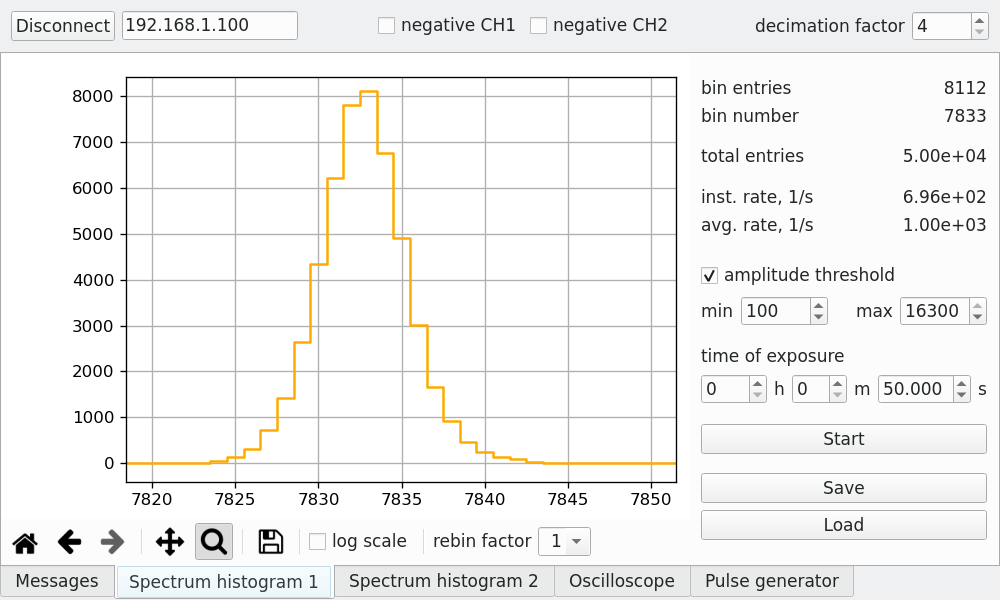
\includegraphics{cap6_mcpha_client}
\caption[GUI de mcpha, de Pavel Demin]{%
Captura de pantalla de la GUI de mcpha, implementada por Pavel Demin para su
versión del MCA~\cite{DeminMCPHA}.\label{f:usr-mcpha}}
\end{figure}

La aplicación realizada en este trabajo, \codigo{mcamon} (por \emph{MCA
monitor}), es una adaptación de esta GUI al HW y SW de este proyecto. Se controla
desde un cliente externo conectado por red, escrito con PyQt5 y matplotlib, que
se conecta con el servidor \codigo{mca\_server.py}. A diferencia de mcpha, el
servidor está escrito en Python: corre en la placa, llama a la API de
adquisición y responde con el protocolo de la Sec.~\ref{S:sw-protocolo-red}.

Casi todas las diferencias con mcpha las imponen los módulos del hardware, que
no es el mismo; se presentan en la Tabla~\ref{t:usr-diferencias-mcpha}.

% [H]: es lo último del capítulo; como float quedaba solo detrás de las referencias.
\begin{table}[H]
\centering
\caption[Diferencias entre mcpha y la aplicación de este trabajo]{%
Diferencias entre mcpha y la aplicación de este
trabajo.\label{t:usr-diferencias-mcpha}}
\begin{tabularx}{\textwidth}{|>{\raggedright\arraybackslash}p{0.36\textwidth}%
  |>{\raggedright\arraybackslash}X|}
\hline \encabezado \textbf{mcpha} & \textbf{Este trabajo} \\ \hline
Dos MCA independientes, con una pestaña de espectro cada uno & Un solo MCA, con
  un selector de canal IN1/IN2 \\ \hline
4096 canales fijos & La cantidad de canales se lee del hardware (registro
  \codigo{WIDTHS}); el cliente no la supone \\ \hline
Temporizador de exposición en hardware & Lo implementa un hilo del servidor,
  contra el tiempo vivo \\ \hline
Negador por canal & No hay negador; en su lugar se elige si la amplitud es el
  pico o la integral de carga \\ \hline
--- & Contadores propios:\newline
  \textbullet~Rechazados por amplitud y por forma.\newline
  \textbullet~Apilados y disparos perdidos.\newline
  \textbullet~Tiempos real, vivo y muerto. \\ \hline
--- & Mapa 2D de forma de pulso y su figura de mérito \\ \hline
\end{tabularx}
\end{table}

La interfaz está en inglés y trae las pestañas de la
Tabla~\ref{t:usr-pestanas}; algunas aparecen sólo si el \emph{bitstream} cargado trae el
módulo correspondiente.

% [H]: es lo último del capítulo; como float quedaba solo detrás de las referencias.
\begin{table}[H]
\centering
\caption[Pestañas de la aplicación y su contenido]{%
Pestañas de la aplicación y su contenido.\label{t:usr-pestanas}}
\begin{tabularx}{\textwidth}{|>{\raggedright\arraybackslash}p{0.2\textwidth}%
  |>{\raggedright\arraybackslash}X|}
\hline \encabezado \textbf{Pestaña} & \textbf{Qué contiene} \\ \hline
\textbf{\emph{Messages}} & cada operación y cada error, con su hora \\ \hline
\textbf{\emph{Spectrum}} & el histograma 1D; la tasa de entrada instantánea y media;
  los contadores (aceptados, rechazados, apilados, perdidos); el tiempo real,
  vivo y muerto; los botones \emph{Start}, \emph{Stop}, \emph{Clear} y de guardado; la lista de picos
  con su FWHM y resolución \\ \hline
\textbf{MCA \emph{settings}} & la franja del MCA, con la tasa y las pérdidas de cada
  etapa; abajo, los registros agrupados por función: preprocesamiento,
  segmentación y ranuras, publicación \\ \hline
\textbf{2D \emph{map} (PSD)} & el mapa de amplitud $\times$ factor de forma
  ($Q_\text{tail}/Q_\text{total}$) y la figura de mérito \\ \hline
\textbf{\emph{Integration}} & de qué punto de la cadena de procesamiento toma sus
  muestras cada consumidor (OSC, multitrigger, MCA, \codigo{event\_ring}) y el
  control global de todo el sistema (\emph{run}, \emph{clear}, \emph{reset}) \\ \hline
\textbf{\emph{Pulses}} & las capturas del osciloscopio, como pulso o como mapa de
  calor, y la tasa en el tiempo \\ \hline
\textbf{OSC \emph{settings}} & la franja del osciloscopio (y la del \emph{ring}, si el
  \emph{bitstream} lo trae), los registros por etapa y la adquisición del \emph{ring} a una
  carpeta de la placa \\ \hline
\textbf{Multitrigger} & la franja del disparo: las fuentes (nivel, pendiente,
  polo-cero), las máscaras OR por canal y el \emph{shield} \\ \hline
\textbf{\emph{Generator}} & el generador de pulsos por etapas (disparos, amplitud,
  forma, salida) y el lazo digital hacia el MCA \\ \hline
\textbf{\emph{Calibration}} & la medición del canal analógico con una referencia
  conocida (\emph{offset}, ruido, ganancia, caída lenta, ancho de banda, diafonía) y la
  base dinámica del MCA \\ \hline
\end{tabularx}
\end{table}

En el Apéndice~\ref{C:ap-app} aparecen capturas de cada una de las pestañas.

% Bibliografía de este capítulo. Va al final del archivo, siempre.
\bibliografiacapitulo

%%% Local Variables:
%%% mode: latex
%%% TeX-master: "template"
%%% End:
      % Tipos de usuario y aplicación (archivo cap6, capítulo 1)
% Origen: Secciones/PI - Analizador Multicanal.md
\chapter{Analizador multicanal}
\label{C:mca}

% Figuras de ESTE capítulo + las compartidas. Siempre al principio del archivo.
\graphicspath{{figs/cap1/}{figs/comunes/}}

En este capítulo describimos qué es un analizador multicanal (MCA), para qué se
lo emplea y qué lugar ocupa en la cadena de medición. Presentamos la
distribución diferencial de alturas, que es la salida del instrumento, y las
etapas del procesamiento digital de cada evento: la apertura, el cierre, el
cálculo de los estadísticos y su publicación al histograma. Después repasamos
los efectos que distorsionan la medición y que el sistema tiene que compensar o,
al menos, reportar: el apilamiento, el \emph{amplitude walk} y el tiempo muerto.
Para este último mostramos por qué hace falta conocerlo con precisión: la
corrección de la tasa amplifica cualquier error en el tiempo muerto, y tanto más
cuanto mayor es la tasa. Cerramos con las figuras de mérito con que se
caracteriza un MCA y con la extensión del histograma a dos dimensiones.

%%%%%%%%%%%%%%%%%%%%%%%%%%%%%%%%%%%%%%%%%%%%%%%%%%%%%%%%%%%%%%%%%%%%%%%%%%%%%%%%
\section{Descripción mínima}
\label{S:mca-descripcion-minima}

La creación de esta herramienta fue el objetivo primordial de este proyecto. Un
MCA construye un \textbf{histograma} de uno o más \emph{estadísticos} de los
pulsos electrónicos; los más utilizados son la altura máxima y la carga
(integral). A pesar de su nombre, un multicanal no necesariamente tiene
múltiples canales: el nombre proviene de un detalle de su implementación
histórica, que se describe en la Sec.~\ref{S:mca-origen-nombre}.

En la Fig.~\ref{f:mca-senal} se presenta su funcionamiento sobre una traza
simulada de la señal cuantizada por un conversor analógico-digital (ADC). El
primer eslabón es el disparador, también llamado \emph{trigger}, con
histéresis: cuando la señal supera un umbral de disparo (\codigo{thr}) se abre
una ventana, que se mantiene abierta hasta que la señal cae por debajo de un
umbral de relajación (\codigo{thr}~$-$~\codigo{hyst}). En la figura el primer
umbral se representa con una línea roja rayada y el segundo con una línea roja
punteada; todas las ventanas (en amarillo) empiezan y terminan donde la curva
corta la línea del umbral correspondiente. Los pulsos que no superan el umbral,
como el \#6, no abren ninguna ventana y no producen ninguna cuenta.

\begin{figure}[H]
\centering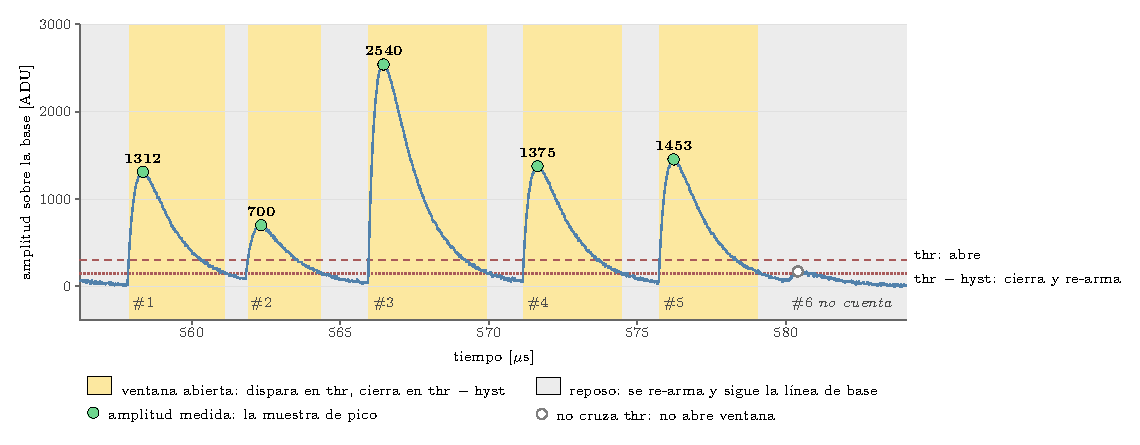
\includegraphics{cap1_senal}
\caption[Funcionamiento esquemático del MCA sobre una traza simulada]{%
Funcionamiento esquemático del MCA sobre una traza simulada con seis pulsos. En
amarillo, la ventana abierta: dispara al cruzar \codigo{thr} y cierra al bajar
de \codigo{thr}~$-$~\codigo{hyst}. En gris, el reposo: el disparador se re-arma
y el seguidor de línea de base actualiza la referencia contra la que se mide la
amplitud. En verde, la amplitud medida de cada pulso.\label{f:mca-senal}}
\end{figure}

Conceptualmente, al cerrarse la ventana tenemos un vector con todas las muestras
del evento, que se transfiere a un extractor de características que calcula
todos los estadísticos en paralelo. En el hardware los estadísticos se calculan
muestra a muestra mientras la ventana está abierta, sin guardar el vector (ver
Sec.~\refpend{S:implmca-recuperacion}{Implementación del MCA: métodos de
recuperación del pulso}). En la Fig.~\ref{f:mca-senal} se presenta únicamente la
altura máxima, con un punto verde en el ápice de cada pulso.

Cada vez que se cierra una ventana, el valor del estadístico se transfiere al
histograma, que suma una cuenta en el canal (o \emph{bin}) correspondiente. A
este mecanismo lo llamamos \emph{publicación} del estimador. En la
Fig.~\ref{f:mca-camino-datos} se presenta este camino de datos: por cada pulso
aceptado viaja un único número, su amplitud, y el histograma suma una cuenta en
el canal \codigo{amp\,\textgreater\textgreater\,6}. El desplazamiento a la
derecha divide la amplitud por $2^6 = 64$, de modo que el rango de 0 a
4095~ADU se agrupa en 64 canales. La tabla inferior lista los pulsos de la
Fig.~\ref{f:mca-senal} tal como los ve el histograma; el \#6 figura como
rechazado porque no superó el umbral. Los detalles del mecanismo de
transferencia de datos para el cálculo del estadístico y su publicación se
presentan en los capítulos de implementación de HW.

\begin{figure}[H]
\centering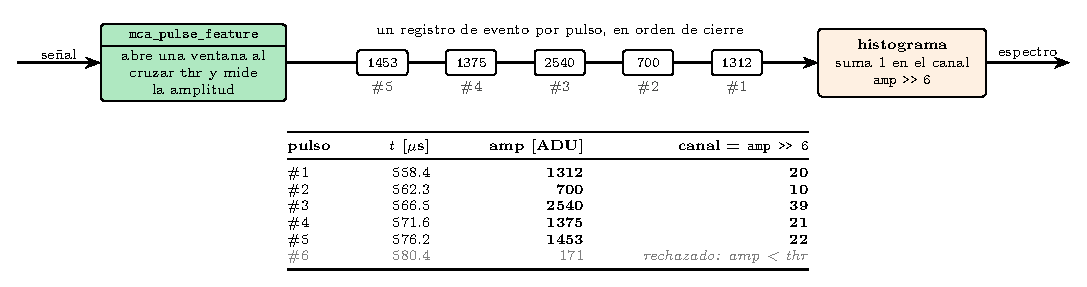
\includegraphics{cap1_camino_datos}
\caption[Camino de datos del MCA]{%
Camino de datos del MCA: un registro de evento por pulso, en orden de cierre, y
la tabla de los pulsos de la Fig.~\ref{f:mca-senal} con su tiempo, su amplitud y
su canal.\label{f:mca-camino-datos}}
\end{figure}

Al acumular las cuentas en un buffer en memoria construimos la
\textbf{distribución diferencial de alturas} ($dN/dH$), que presentamos en la
próxima subsección y que es la salida del módulo. En la
Fig.~\ref{f:mca-histograma} se presenta el espectro final, con la evolución de
la acumulación en barras apiladas: la capa inferior corresponde a las primeras
12 cuentas, la del medio a las cuentas 13 a 64 y la superior a las cuentas 65 a
227. El borde superior de cada capa es el espectro en ese instante. Con las
primeras 12 cuentas no se puede afirmar nada; recién con la acumulación completa
las dos líneas del espectro se distinguen como líneas. A la izquierda del umbral
\codigo{thr} el espectro está vacío por construcción, y no por falta de
estadística.

\begin{figure}[H]
\centering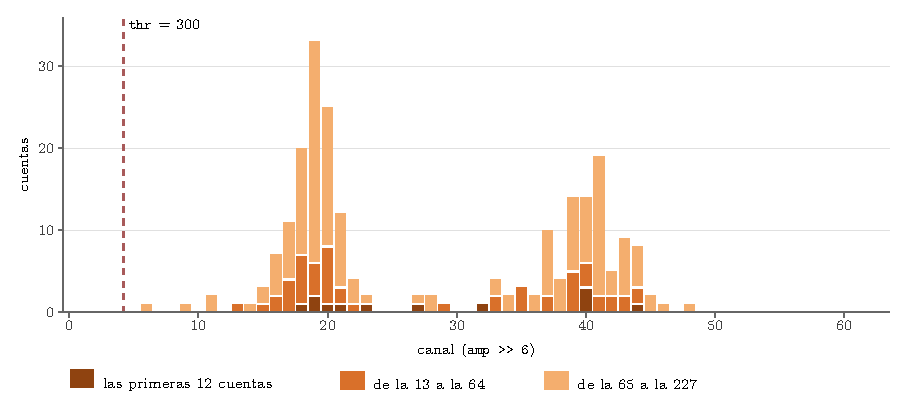
\includegraphics{cap1_histograma}
\caption[Espectro final y evolución de la acumulación]{%
Espectro final en barras apiladas, una capa por tramo de la acumulación: hasta
12, 64 y 227 cuentas. La línea roja marca el umbral \codigo{thr} sobre el eje de
amplitud.\label{f:mca-histograma}}
\end{figure}

Como cada canal es un acumulador, las cuentas del histograma crecen con el
tiempo, a menos que se las reinicie de forma manual.

\subsection{Distribución diferencial de alturas}
\label{S:mca-dda}

La salida del MCA es la \textbf{distribución diferencial de alturas} (DDA), que
escribimos $dN/dH$ (Knoll~\citecap{Knoll2010}{4}). Si $H$ es la altura del pulso
(o el estadístico que se esté histogramando), $dN/dH$ es la cantidad de pulsos
por unidad de altura alrededor de $H$. La cantidad de pulsos con alturas entre
$H_1$ y $H_2$ es su área,
\begin{equation}
  N_{[H_1,\,H_2]} = \int_{H_1}^{H_2} \frac{dN}{dH}\,dH ,
  \label{e:mca-area}
\end{equation}
y el área total, $N_0 = \int_0^{\infty} \frac{dN}{dH}\,dH$, es la cantidad
total de pulsos registrados. En el MCA la altura está discretizada en canales de
ancho $\Delta H$: la integral se vuelve una suma y la cuenta del canal $i$ es
$N_i \simeq \frac{dN}{dH}(H_i)\,\Delta H$. Es una medición de la distribución de
probabilidad de las alturas, sin normalizar: dividiendo por $N_0\,\Delta H$ se
obtiene la densidad de probabilidad.

Su contraparte es la \textbf{distribución integral de alturas} $N(H)$, la
cantidad de pulsos con altura mayor que $H$, que se relaciona con la diferencial
por $dN/dH = -dN(H)/dH$. Es lo que mide un único discriminador con su umbral en
$H$ seguido de un contador, como en la cadena analógica de la
Fig.~\ref{f:mca-cadena-analogica}. No la utilizamos: en la distribución
diferencial las líneas se ven como picos, y su posición, su ancho y su área se
leen de forma directa. Por eso, cuando hablamos del histograma o del espectro
nos referimos siempre a $dN/dH$.

\subsection{Origen histórico del nombre}
\label{S:mca-origen-nombre}

Históricamente, este tipo de análisis empleaba un banco de dispositivos
analógicos llamados \emph{Single Channel Analyzer} (SCA). Cada SCA cuenta los
pulsos cuya altura cae dentro de una ventana fija $[H, H + \Delta H]$,
delimitada por un discriminador inferior y uno superior, de modo que mide un
punto de la distribución diferencial. Cada uno de estos dispositivos se
denominaba canal, y la configuración de múltiples de ellos con ventanas
contiguas, que mide la curva entera de una vez, se llamó \textbf{Multichannel
Analyzer} (MCA). Este esquema se presenta en la Fig.~\ref{f:mca-sca}.

\begin{figure}[H]
\centering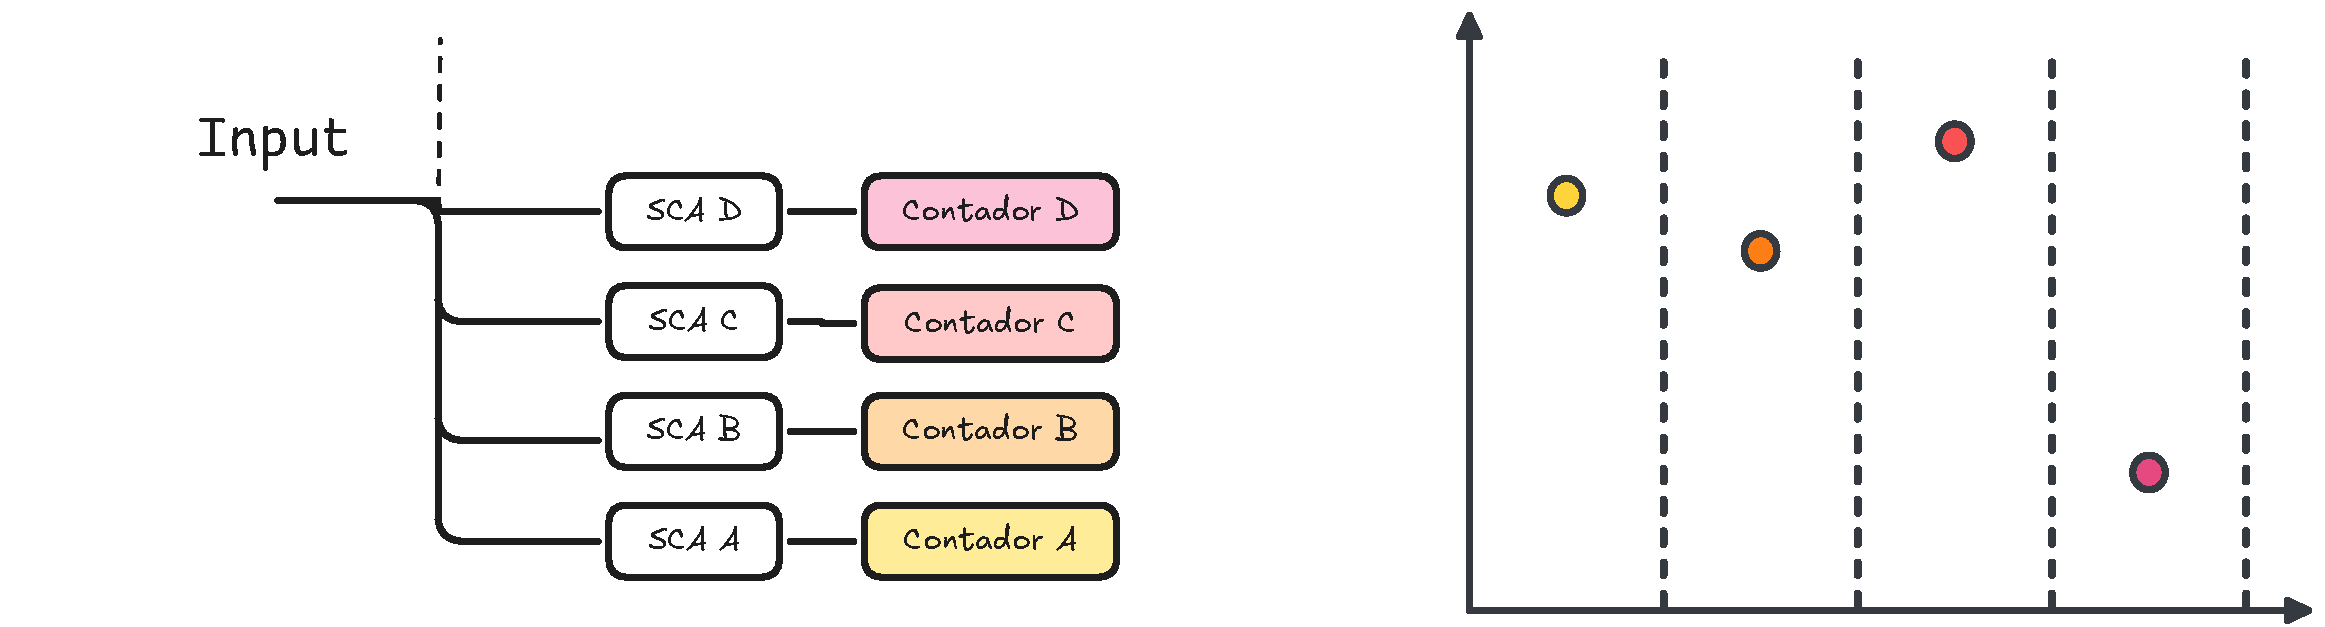
\includegraphics{cap1_sca_mca}
\caption[Un MCA como banco de SCA]{%
Un MCA como banco de SCA: todos reciben la misma entrada y cada uno alimenta a
su propio contador.\label{f:mca-sca}}
\end{figure}

Agregar canales lleva a un muestreo cada vez más fino del espectro continuo,
pero aumenta la varianza relativa de cada canal, porque cada uno recibe menos
cuentas.

En la Fig.~\ref{f:mca-bines} se presentan mediciones con la misma cantidad total
de cuentas del espectro continuo mostrado en (a), variando la cantidad de
canales (o \emph{bines}) utilizados. En (b) la cantidad de canales es demasiado
pequeña para mostrar detalle suficiente; en (c) tenemos la elección que busca un
punto medio entre resolución y fluctuación estadística; y en (d) tenemos tantos
canales que las fluctuaciones estadísticas son tan grandes que podrían
enmascarar picos pequeños. El extremo de pocos canales está acotado por la
corrección de Sheppard~\cite{Sheppard1898}: un canal de ancho $\Delta$ suma
$\Delta^2/12$ a la varianza del pico, y para que no la infle en más de
$\sim$\qty{1}{\percent} hacen falta al menos 4 canales por FWHM. Se detalla en
el Apéndice~\refpend{S:implmca-fisher-bineado}{Poder resolutivo de Fisher en la
elección del bineado}.

\begin{figure}[H]
\centering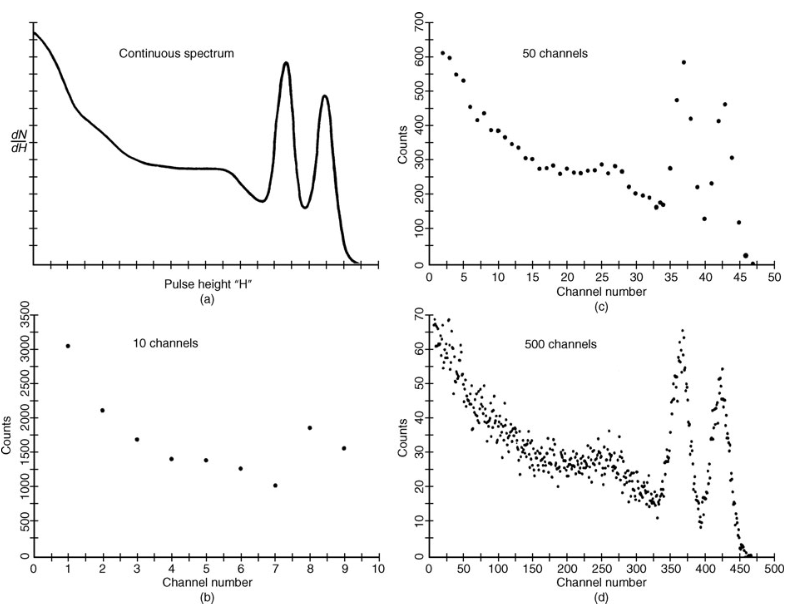
\includegraphics{cap1_bines_knoll}
\caption[Efecto de la cantidad de canales sobre un mismo espectro]{%
Efecto de la cantidad de canales sobre un mismo espectro con igual cantidad
total de cuentas. Extraída de Knoll~\cite[cap.~18, pág.~707]{Knoll2010}.
\label{f:mca-bines}}
\end{figure}

%%%%%%%%%%%%%%%%%%%%%%%%%%%%%%%%%%%%%%%%%%%%%%%%%%%%%%%%%%%%%%%%%%%%%%%%%%%%%%%%
\section{Descripción práctica}
\label{S:mca-descripcion-practica}

En esta sección describimos el \textbf{acercamiento que tiene un nuevo usuario}
frente a este tipo de dispositivos. La idea de este proyecto fue obtener una
versión con el \textbf{mismo conjunto de funcionalidades mínimas} que los
equipos comerciales. Estas funcionalidades deberían incluir al menos:
\begin{itemize}
  \item Capacidad de control de la adquisición: \textbf{reiniciar las cuentas
    presentes} y decidir cuándo \textbf{arrancar y detener la adquisición}.
  \item Capacidad de visualizar el espectro en tiempo real.
  \item \textbf{Guardar} los datos presentes.
  \item Algún sistema de \textbf{advertencia} para indicar \textbf{operación
    fuera de los límites de la especificación} obtenida.
\end{itemize}

En la Fig.~\ref{f:mca-amptek} se presenta una de las interfaces gráficas de
usuario (\emph{Graphical User Interface}, GUI) a las que buscamos acercarnos en
este trabajo. La misma cuenta con:
\begin{itemize}
  \item el espectro, en escala logarítmica y calibrado en energía, con regiones
    de interés (ROI) resaltadas;
  \item la configuración del equipo: cantidad de canales, umbral inferior (LLD),
    tiempo de pico del conformado y ganancia;
  \item el estado de la adquisición: cuentas totales, tasa de entrada, tiempo
    muerto y tiempo de acumulación;
  \item la información del pico seleccionado: centroide, FWHM, área neta con su
    incerteza e identificación de la línea;
  \item la temperatura y la alta tensión del detector.
\end{itemize}

\begin{figure}[H]
\centering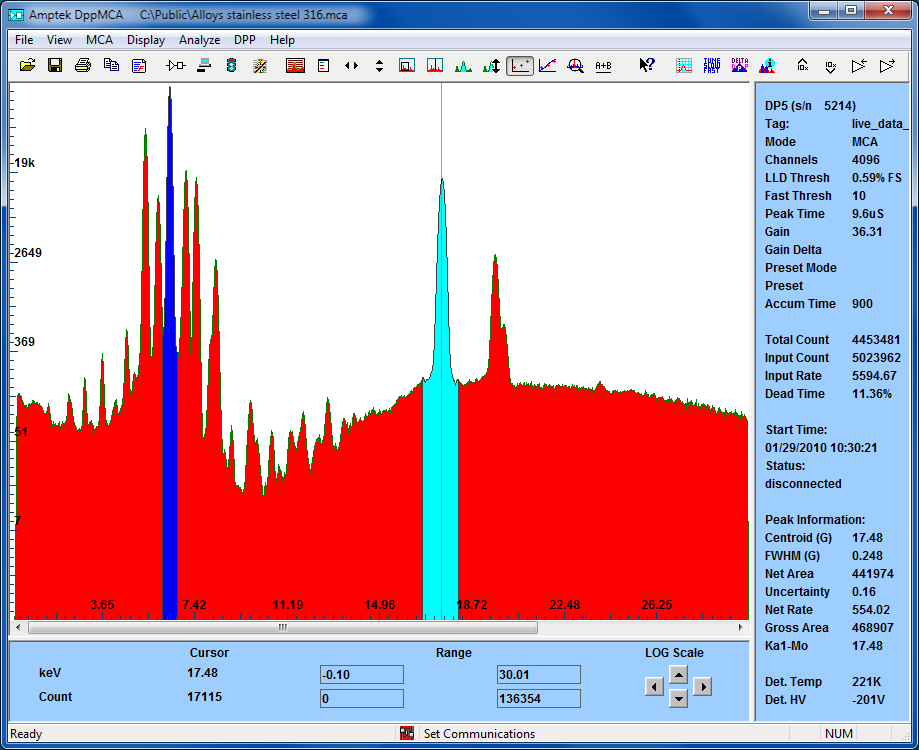
\includegraphics[width=0.6\linewidth]{cap1_amptek_dppmca}
\caption[Software DppMCA del MCA comercial de Amptek]{%
Captura del software propietario que acompaña al MCA comercial de Amptek
(DppMCA)~\cite{AmptekDPPMCA}.\label{f:mca-amptek}}
\end{figure}

La aplicación desarrollada en este trabajo se presenta en la
Sec.~\ref{S:usr-app}.

%%%%%%%%%%%%%%%%%%%%%%%%%%%%%%%%%%%%%%%%%%%%%%%%%%%%%%%%%%%%%%%%%%%%%%%%%%%%%%%%
\section{Cadena de medición típica}
\label{S:mca-cadena-medicion}

El MCA es el \emph{último eslabón} de la cadena de adquisición de un esquema
experimental. Históricamente esta cadena tiene las etapas que se presentan
esquemáticamente en la Fig.~\ref{f:mca-cadena-medicion}:
\begin{enumerate}
  \item \textbf{Detector}:
  \begin{enumerate}
    \item Es el elemento en el que la radiación interactúa y deposita su
      energía. En el Apéndice~\ref{S:ap-detectores} se presenta una tabla con
      las familias de detectores, sus funcionalidades y sus parámetros
      importantes.
    \item El modelo más sencillo lo considera una \textbf{fuente de corriente}:
      cada interacción libera una carga $Q$, proporcional a la energía
      depositada, durante un tiempo de colección que va de nanosegundos a
      microsegundos según el detector. La información de la energía está en la
      carga, $Q = \int i_{sig}(t)\,dt$, y no en la forma del pulso de corriente.
    \item Requiere una \textbf{polarización} (\emph{bias}) de alta tensión, que
      fija la ganancia y el ruido paralelo por corriente de fuga.
  \end{enumerate}
  \item \textbf{Preamplificador}:
  \begin{enumerate}
    \item Su función principal es convertir la \textbf{carga} en
      \textbf{tensión} con la mejor relación señal a ruido (SNR) posible. Por eso
      se lo ubica lo más cerca posible del detector.
    \item Lleva la señal del detector a un rango dinámico en el que las etapas
      siguientes trabajan con mejor precisión.
    \item En la versión sensible a la carga, la salida es un escalón de altura
      $\Delta V = Q/C_F$, con una subida que sigue a la colección de carga y una
      caída exponencial lenta, de constante $R_F C_F$. El tiempo de subida es
      mucho más rápido que el de bajada.
  \end{enumerate}
  \item \textbf{Amplificador de conformado} (\emph{shaping amplifier}):
  \begin{enumerate}
    \item Generalmente contiene una cancelación polo-cero previa, que evita el
      sobreimpulso negativo (\emph{undershoot}) que deja la cola del
      preamplificador al diferenciarla.
    \item Modifica la señal analógica para acortarla, de modo que las colas de
      pulsos sucesivos no se acumulen, y para llevarla a un rango de tensión
      adecuado para las entradas analógicas convencionales.
    \item La elección del filtro fija el \textbf{ancho de banda} del estimador
      de amplitud y, con él, el compromiso entre el ruido serie y el paralelo
      (ver Sec.~\ref{S:mca-tipos-conformado}).
  \end{enumerate}
  \item \textbf{Discriminador o trigger}: decide qué pulsos son eventos. Dispara
    cuando la señal conformada cumple una condición, típicamente superar un
    umbral, y descarta el ruido y los pulsos de baja amplitud. Su salida puede
    ir a un contador, que mide la cantidad de eventos o la tasa, o a un MCA, que
    mide el espectro de energía.
  \item \textbf{Analizador multicanal}:
  \begin{enumerate}
    \item \textbf{Conversión A-D}: transforma la señal analógica mediante una
      cuantización doble. La primera es en tiempo, en la que se suele tener un
      muestreo periódico; la segunda es en valor, para la cual se elige un
      código digital.
    \item \textbf{Restaurador de línea de base}: estima el nivel sobre el que
      monta cada pulso y lo resta, para que la altura medida no dependa de los
      pulsos anteriores ni de derivas lentas.
    \item \textbf{Determinación de eventos}: decide dónde empieza y dónde
      termina cada evento (ver Sec.~\ref{S:mca-etapas}).
    \item \textbf{Cálculo de estadísticos}: calcula la altura, la carga u otros
      estadísticos de cada evento.
    \item \textbf{Discriminador}: decide si el evento entra o no al histograma,
      comparando uno de sus estadísticos contra un intervalo.
    \item \textbf{Contador (histograma)}: suma una cuenta en el canal que
      corresponde al estadístico del evento.
  \end{enumerate}
\end{enumerate}

\begin{figure}[H]
\centering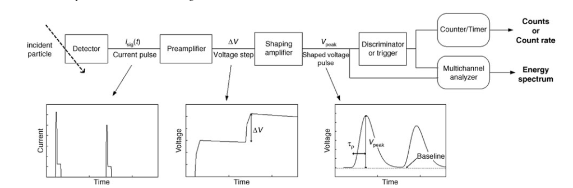
\includegraphics{cap1_cadena_medicion}
\caption[Cadena de medición típica]{%
Cadena de medición típica: detector, preamplificador, amplificador de conformado
y discriminador, seguidos de un contador o de un MCA.\label{f:mca-cadena-medicion}}
\end{figure}

Históricamente, cada una de estas etapas, hasta la discriminación, tenía una
correspondencia directa con un circuito analógico. En la
Fig.~\ref{f:mca-cadena-analogica} se presenta una implementación simple: un
detector de ionización seguido de un preamplificador sensible a la carga, al que
le sigue un amplificador de conformado CR-RC (un pasaaltos, una ganancia y un
pasabajos en cascada) y, a continuación, un detector de eventos por nivel
implementado con un comparador de umbral $V_{LLD}$, cuya salida se lleva a un
contador.

\begin{figure}[H]
\centering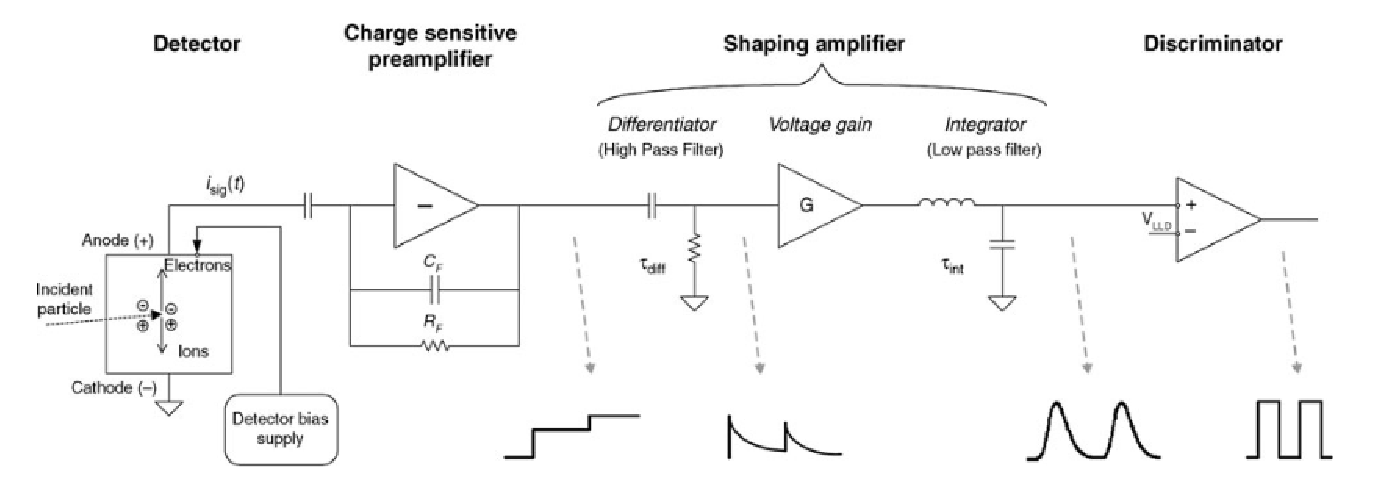
\includegraphics{cap1_cadena_analogica_mca}
\caption[Electrónica simple de procesamiento de señal de un detector]{%
Electrónica simple de procesamiento de señal de un detector. Extraída de
Knoll~\citefig{Knoll2010}{16.2}.\label{f:mca-cadena-analogica}}
\end{figure}

Como el comparador evalúa únicamente la condición $V > V_{LLD}$, las cuentas
resultantes representan la distribución integral de alturas, $N(V_{LLD})$ (ver
Sec.~\ref{S:mca-dda}). Para obtener el espectro hay que barrer el umbral o
reemplazar el comparador por un banco de canales.

En la actualidad, con hardware de tasas de adquisición suficientemente altas en
términos de muestras por pulso (por ejemplo, más de 10), obtenemos un grado de
recuperación digital del pulso que permite emplear técnicas de procesamiento
digital de señales (DSP). Aunque el filtrado de conformado puede implementarse
digitalmente, una etapa analógica previa al ADC sigue siendo necesaria por las
siguientes razones:
\begin{itemize}
  \item \textbf{Rango dinámico y apilamiento}: la señal del preamplificador
    presenta colas exponenciales de decenas de \unit{\micro\second}. A tasas
    altas, estas colas se acumulan (\emph{pileup}) y desplazan la línea de base,
    lo que puede saturar el ADC. La cancelación polo-cero y el acortamiento
    analógico del pulso mantienen la señal acotada. Esto debe hacerse antes de
    digitalizar, porque una saturación no puede corregirse después.
  \item \textbf{Consideraciones de ruido}:
  \begin{enumerate}
    \item \textbf{Antialiasing}: el muestreo exige que la entrada al ADC no
      tenga contenido por encima de $f_s/2$ (teorema de
      Nyquist~\citecap{Oppenheim2010}{4}). El ruido de banda ancha del
      preamplificador que supera ese límite se pliega dentro de la banda útil, y
      ningún filtro digital posterior puede separarlo. Esto requiere un
      pasabajos analógico, aunque no necesariamente un conformador completo.
    \item \textbf{Ruido de digitalización}: el ruido propio del ADC
      (cuantización, ruido térmico) es fijo en LSB y se suma en cuadratura al
      del detector. Una ganancia analógica $G$ previa lo reduce en un factor $G$
      cuando se lo refiere a la entrada, de modo que la resolución queda
      limitada por el ruido del detector y no por el del ADC. La ganancia está
      acotada por el rango dinámico: el pulso máximo, más la excursión de la
      línea de base, no debe saturar el conversor.
  \end{enumerate}
\end{itemize}

De forma que la cadena utilizada en este proyecto se aproxima a la presentada en
la Fig.~\ref{f:mca-cadena-pitaya}: la señal del amplificador de conformado entra
a la Red Pitaya~\cite{RedPitayaDocs} por su entrada analógica (IN), y todos los
elementos posteriores tienen lugar en el dominio digital. Además, el sistema
digital retoma parte del conformado: la cancelación polo-cero y el conformado
trapezoidal digitales~\cite{Jordanov1994} (ver
Sec.~\refpend{S:implmca-trapezoidal}{Implementación del MCA: recuperación por
conformación trapezoidal}).

\begin{figure}[H]
\centering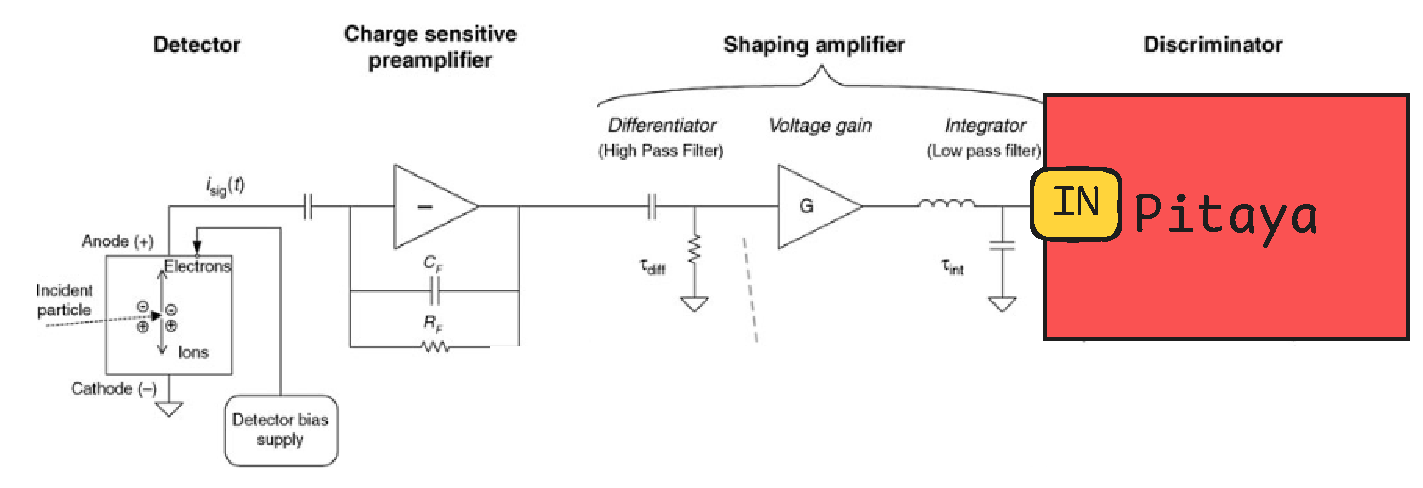
\includegraphics{cap1_cadena_pitaya}
\caption[Cadena de medición utilizada en este trabajo]{%
Cadena utilizada en este trabajo sobre el esquema de la
Fig.~\ref{f:mca-cadena-analogica}: el sistema digital adopta parte de la
conformación de pulsos, la discriminación y el conteo.\label{f:mca-cadena-pitaya}}
\end{figure}

Como este procesamiento previo fija la forma de los pulsos que llegan al MCA, en
la siguiente sección se exploran las diferentes variantes de conformado.

\subsection{Tipos de conformado}
\label{S:mca-tipos-conformado}

En la fase de conformación se aplica algún \textbf{amplificador de conformado}
(Knoll~\citecap{Knoll2010}{16}). En la Fig.~\ref{f:mca-familias} se presentan
las seis familias de conformado de pulsos más aplicadas históricamente,
sintetizadas a partir de su expresión analítica con un ancho a media altura
FWHM~=~\qty{2}{\micro\second} y una altura máxima $A = \qty{0.25}{\volt}$. Son
las formas que usamos como estímulo en las pruebas con el generador de
funciones.

\begin{figure}[H]
\centering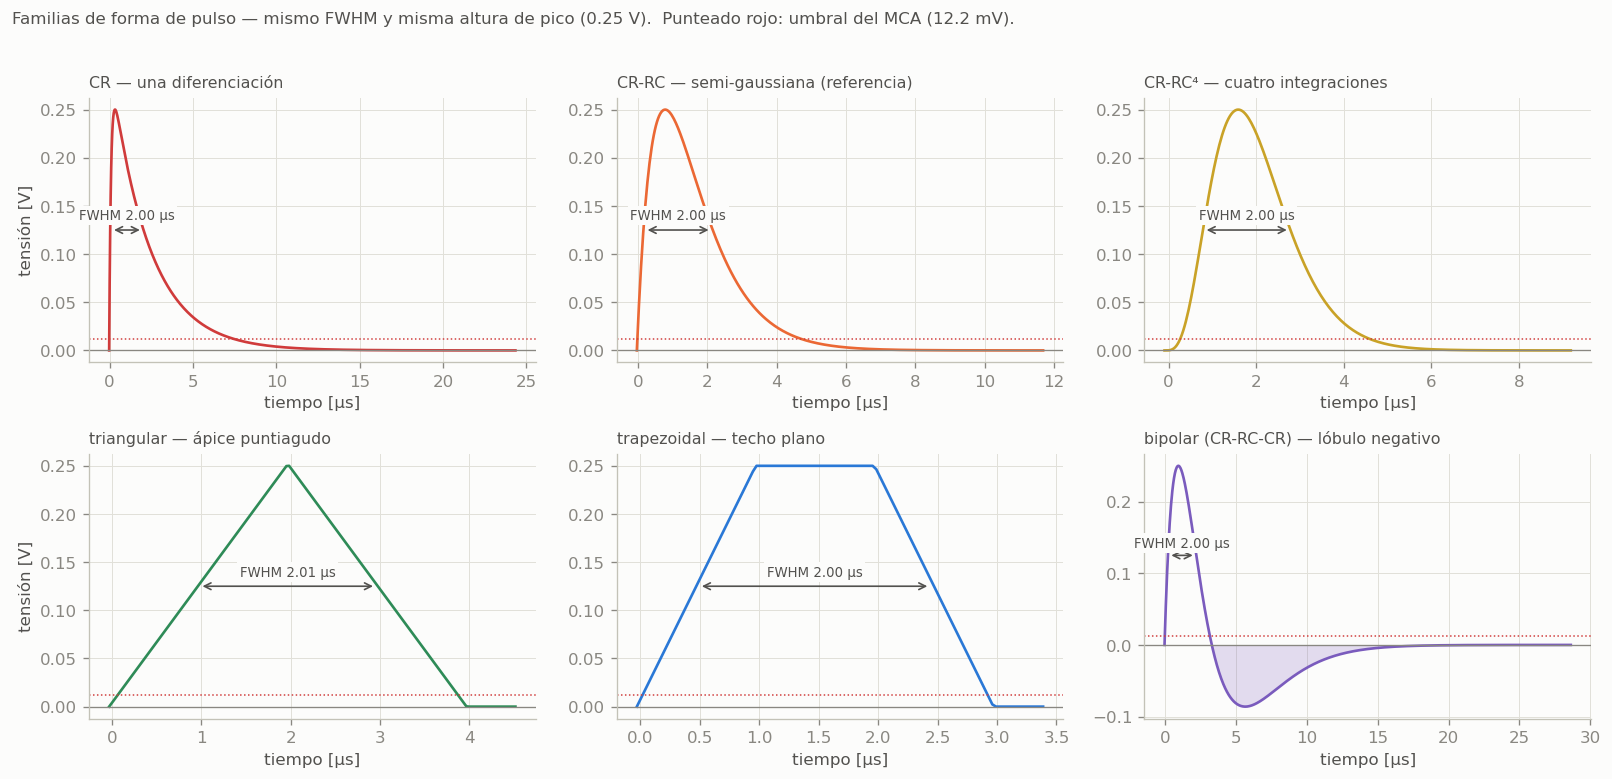
\includegraphics{cap1_familias_conformado}
\caption[Las seis familias de conformado]{%
Las seis familias de conformado, con el mismo FWHM y la misma altura máxima.
\label{f:mca-familias}}
\end{figure}

Estas pueden aproximarse con funciones analíticas $f(u)$, con $u$ el tiempo
normalizado por la constante de tiempo del conformador. Sus características
cualitativas se presentan en la Tabla~\ref{t:mca-conformados}.

\begin{table}[H]
\centering
\caption[Familias de conformado principales]{%
Familias de conformado principales empleadas antes de un MCA.
\label{t:mca-conformados}}
\renewcommand{\arraystretch}{1.6}
\begin{tabular}{|l|l|}
\hline
\encabezado \textbf{Familia} & \textbf{$f(u)$} \\ \hline
\codigo{cr} & $\left(1 - e^{-u/r}\right)e^{-u}$, \ $r = 0.05$ \\ \hline
\codigo{cr\_rc} & $u\,e^{-u}$ \\ \hline
\codigo{cr\_rc4} & $\dfrac{u^{n}e^{-u}}{n!}$, \ $n = 4$ \\ \hline
\codigo{triangular} & $u$ en $[0,1]$; \ $2-u$ en $(1,2]$ \\ \hline
\codigo{trapezoidal} & $u$ en $[0,1]$; \ $1$ en $(1,1{+}p]$; \ $2{+}p-u$ después; \ $p = 1$ \\ \hline
\codigo{bipolar} & $\left(1-\dfrac{u}{2}\right)u\,e^{-u}$ \\ \hline
\end{tabular}
\end{table}

La forma del pulso no es indiferente para el MCA: cada una de las compensaciones
internas se apoya en alguna propiedad de la forma, y la que favorece a una puede
perjudicar a otra.
\begin{itemize}
  \item \textbf{Estimador de altura máxima}: importa cuánto dura el ápice. El
    trapecio mantiene el máximo durante toda su meseta y el ADC lo muestrea
    muchas veces; la CR y la triangular tienen un ápice de pocas muestras, y la
    altura medida depende de la fase del muestreo respecto del pico.
  \item \textbf{Pérdida balística} (\emph{ballistic deficit}): es la parte de la
    amplitud que se pierde porque la carga del detector no llega de golpe. Si el
    tiempo de colección $t_c$ no es despreciable frente al tiempo de conformado,
    el conformador empieza a decaer antes de que termine de llegar la carga, y
    la altura que entrega es menor que la de un escalón de la misma carga
    (Knoll~\citecap{Knoll2010}{17}). Si $t_c$ cambia de un pulso a otro, por
    ejemplo según dónde interactúa la radiación en el detector, la pérdida
    también cambia y ensancha el pico. La sufren más las formas de ápice corto,
    como la CR-RC y la triangular; el trapecio la tolera mientras su meseta dure
    más que $t_c$.
  \item \textbf{Ruido}: si el ruido dominante entra antes del conformador, como
    el del preamplificador, el orden lo da la relación señal a ruido de
    Nicholson~\cite{Nicholson1974} (reproducida en
    Knoll~\citecap{Knoll2010}{17}): la triangular y la CR-RC$^4$ se acercan al
    filtro óptimo (\emph{cusp}) y la CR-RC queda bastante atrás. Si el ruido
    dominante es el del ADC, que entra después del conformador, el orden se
    invierte para el estimador de altura máxima: el trapecio pasa a ser el mejor
    y la triangular, uno de los peores.
  \item \textbf{Estimadores de carga y de forma}: el cociente entre la carga y
    la altura, que usamos como factor de forma, depende de cuánta cola tiene el
    pulso. Con el mismo FWHM vale $\approx 1.34$ para la CR y $1.00$ para el
    trapecio, así que un corte por forma calibrado con una familia no sirve para
    otra.
  \item \textbf{Apilamiento y línea de base}: las colas largas (CR, CR-RC,
    CR-RC$^4$) mantienen la señal lejos de la línea de base durante más tiempo
    y, a una tasa dada, aumentan la probabilidad de que el pulso siguiente monte
    sobre ellas. Un seguidor IIR de la línea de base se ajusta bien a una cola
    exponencial, y el conformado trapezoidal digital~\cite{Jordanov1994} la
    cancela cuando se conoce su constante de tiempo.
  \item \textbf{Pulsos bipolares}: el lóbulo negativo hace que el área neta del
    pulso sea cero y evita que la línea de base se corra con la tasa, pero un
    estimador que recorta la señal a valores positivos pierde la mitad del área,
    y la segmentación de eventos se complica.
  \item \textbf{Disparo}: las formas de subida lenta, como la CR-RC$^4$, son las
    que más sufren el \emph{amplitude walk} (ver
    Sec.~\ref{S:mca-amplitude-walk}).
\end{itemize}

%%%%%%%%%%%%%%%%%%%%%%%%%%%%%%%%%%%%%%%%%%%%%%%%%%%%%%%%%%%%%%%%%%%%%%%%%%%%%%%%
\section{Las cuatro etapas de procesamiento digital}
\label{S:mca-etapas}

Podemos subdividir el procesamiento de este módulo en cuatro etapas por evento,
presentadas brevemente en la Sec.~\ref{S:mca-descripcion-minima}:
\begin{enumerate}
  \item \textbf{Identificación del comienzo del evento}.
  \item \textbf{Determinación del final del evento}.
  \item \textbf{Cálculo de estadísticos}.
  \item \textbf{Publicación del estadístico}.
\end{enumerate}

En las siguientes secciones se describen las dos primeras con más detalle. El
cálculo de los estadísticos y su publicación dependen fuertemente de la
arquitectura, y se describen junto con su implementación en el
Cap.~\ref{C:implmca}.

\subsection{Determinación del comienzo del evento}
\label{S:mca-comienzo-evento}

Es el mecanismo con el que determinamos la \textbf{presencia de un evento}. A
estos mecanismos los llamamos \emph{fuentes de disparo}: son señales de control
para el flujo de datos (llamado \emph{datapath}). En nuestro sistema contamos
con múltiples fuentes, que se presentan a continuación:
\begin{itemize}
  \item Triggers por \textbf{condiciones sobre la señal digitalizada por el
    ADC}:
  \begin{itemize}
    \item \textbf{Trigger por nivel} (\emph{level trigger}): dispara cuando la
      señal supera, o baja de, un umbral de tensión específico, con histéresis.
    \item \textbf{Trigger por pendiente} (\emph{slope trigger}): se basa en la
      rapidez de cambio de la señal, de modo que no lo afectan los corrimientos
      lentos de la línea de base.
    \item \textbf{Trigger con polo-cero}: compara contra el umbral la señal con
      la cola del pulso anterior cancelada, de modo que detecta un pulso chico
      montado sobre la cola de uno grande.
    \item Otros tipos habituales en los osciloscopios, como el disparo por ancho
      de pulso o por ausencia de señal (\emph{timeout}), no se implementaron.
  \end{itemize}
  \item \textbf{Trigger digital externo}: utilizamos alguna señal digital
    externa como fuente.
  \item \textbf{Trigger manual}: el disparo se ordena por software.
  \item \textbf{Generador de señales} (ASG): el generador del propio sistema
    marca los momentos de interés de la señal que genera.
\end{itemize}

Las fuentes se pueden combinar: el disparo de cada canal es el OR de las fuentes
habilitadas por una máscara (ver Cap.~\ref{C:multitrigger}).

Una vez determinado el \textbf{inicio} de un evento tenemos que determinar su
final. En la siguiente sección presentamos los criterios de finalización.

\subsection{Determinación del final del evento}
\label{S:mca-final-evento}

Una vez que un disparo abrió la ventana de análisis, hay que decidir cuándo
cerrarla. Implementamos dos métodos:
\begin{enumerate}
  \item \textbf{Por ancho fijo}:
  \begin{itemize}
    \item Damos como parámetro una cantidad $N$ de muestras a analizar.
    \item Es útil cuando la variación del ancho del pulso es pequeña,
      generalmente con una fuente conocida.
    \item Si sobredimensionamos el largo de la ventana podemos bloquear el pulso
      siguiente; si lo subestimamos, no tenemos en cuenta toda la relajación del
      pulso.
  \end{itemize}
  \item \textbf{Por histéresis}:
  \begin{itemize}
    \item Consiste en una ventana de ancho variable, determinada por un
      \textbf{ciclo de histéresis}: cierra cuando la señal cae por debajo del
      umbral de relajación.
    \item Es útil cuando los pulsos tienen anchos variables.
  \end{itemize}
\end{enumerate}

Si aplicamos ambas técnicas a un mismo tren de pulsos obtenemos la
Fig.~\ref{f:mca-politicas-final}, en la que se marca en gris el tiempo con la
ventana abierta. En la primera fila (a), la política de ancho fijo subestima el
ancho de los pulsos: la ventana cierra mientras la cola sigue por encima del
umbral de relajación \codigo{thr\_lo}. Como resultado, el estadístico no tiene
en cuenta esa cola y, además, el disparador no puede re-armarse hasta que la
señal baje. Ese intervalo, rayado en rojo, es tiempo muerto aunque la ventana ya
esté cerrada, y los pulsos que llegan durante él (marcas grises) se pierden sin
que ningún contador los registre. En la segunda fila (b), la ventana por
histéresis dura hasta que la señal baja de \codigo{thr\_lo}: cubre toda la cola
y no deja tiempo bloqueado fuera de la ventana.

\begin{figure}[H]
\centering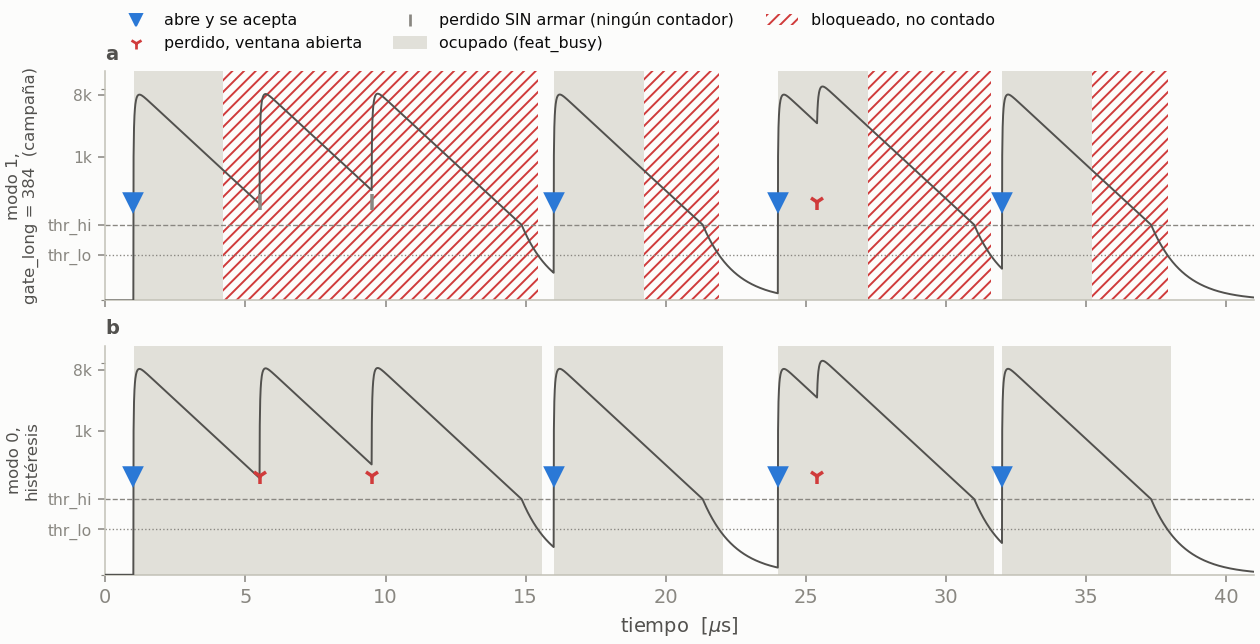
\includegraphics{cap1_politicas_final}
\caption[Criterios de final de evento]{%
Criterios de final de evento sobre el mismo tren de pulsos: (a) política de
ancho fijo, (b) política por histéresis.\label{f:mca-politicas-final}}
\end{figure}

Las marcas rojas señalan una doble falta del sistema ante un pulso que llega con
la ventana abierta. Por un lado, el trigger por nivel no lo detecta, porque la
señal nunca bajó del umbral de re-armado. Por otro, el pulso queda dentro de la
misma ventana: su contribución se suma al estadístico del primero, que pasa a
ser un evento apilado (ver Sec.~\ref{S:mca-pileup}), y con la política por
histéresis además alarga la ventana, porque la señal tarda más en bajar.

Esto obliga a distinguir el \textbf{cierre} de la ventana del
\textbf{re-armado} del disparador. El cierre termina la medición del evento; el
re-armado vuelve a poner disponible el sistema para un nuevo disparo, y en un
disparo por nivel ocurre recién cuando la señal baja de \codigo{thr\_lo}. Con la
ventana por histéresis ambos coinciden, porque ocurren en el mismo nivel; con la
ventana fija no, y entre ambos el sistema queda bloqueado (el intervalo rayado
de la Fig.~\ref{f:mca-politicas-final}). En nuestra implementación ese intervalo
se cuenta por separado (ver Sec.~\refpend{S:implmca-teselado}{Implementación del MCA: teselado del tiempo de adquisición}).

\subsection{\texorpdfstring{\emph{Pileup}}{Pileup}}
\label{S:mca-pileup}

Es la deformación del histograma debida a la \textbf{superposición de pulsos en
la entrada}~\cite{Knoll2010}. Cómo modifica el espectro depende de los
siguientes parámetros:
\begin{enumerate}
  \item La metodología de medición: cómo se abre y se cierra la ventana y qué
    estadístico se calcula (ver Sec.~\ref{S:mca-etapas}).
  \item La distribución de los tiempos entre arribos: para una fuente radiactiva
    los arribos son un proceso de Poisson de tasa $\lambda$,
    $\mathrm{PP}(\lambda)$, y los tiempos entre arribos siguen una exponencial,
    $\mathrm{EXP}(\lambda)$.
  \item La distribución de las alturas de los pulsos superpuestos: las suponemos
    independientes, de modo que el segundo pulso tiene la misma distribución de
    alturas que el primero.
  \item La familia de pulsos (el conformado).
\end{enumerate}

En la Fig.~\ref{f:mca-pileup} comparamos la distribución de alturas ($dN/dH$)
medida para pulsos de dos familias. En la primera fila tenemos un pulso unipolar
con cola positiva, del tipo CR-RC, mientras que en la segunda tenemos un pulso
bipolar, cuya cola es negativa. Cuando el segundo pulso monta sobre la cola del
primero, en el primer caso su altura se sobreestima y aparece un exceso de
cuentas a alturas mayores que la del pico real; en el segundo caso se subestima
y el exceso aparece a alturas menores.

\begin{figure}[H]
\centering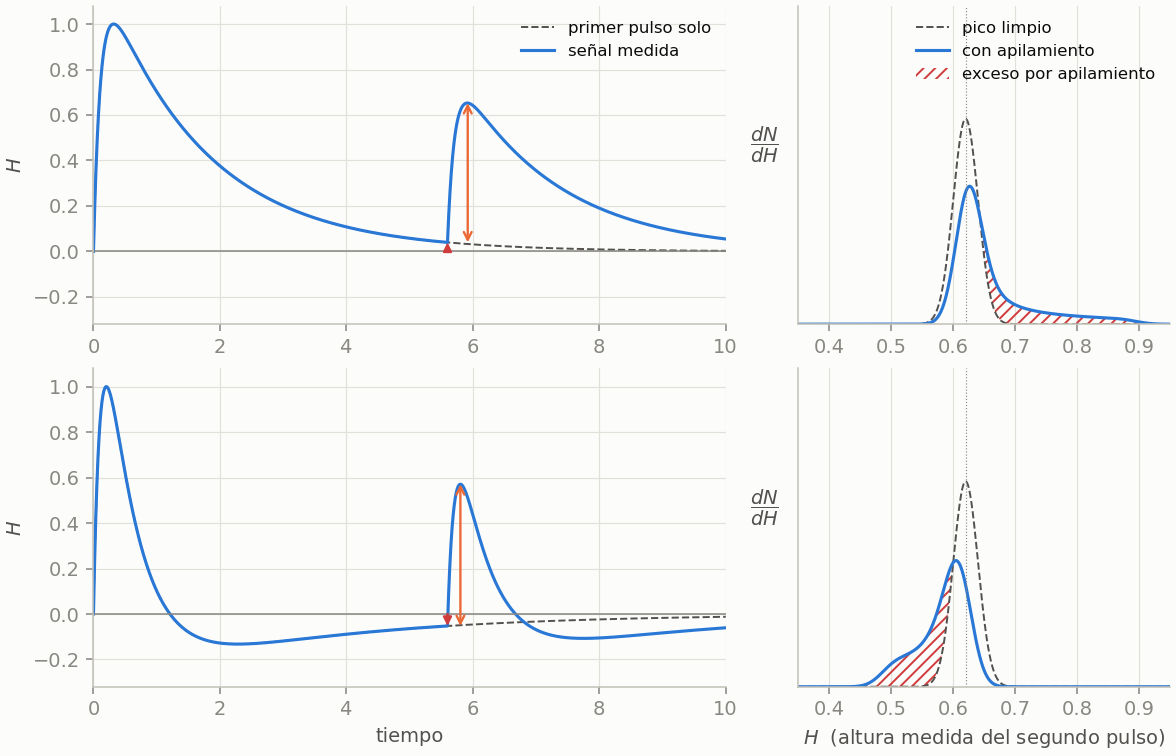
\includegraphics{cap1_pileup}
\caption[Efecto del apilamiento sobre la altura medida]{%
Efecto del apilamiento sobre la altura medida del segundo pulso. Izquierda: la
señal medida y el primer pulso solo; la flecha es la altura medida del segundo.
Derecha: $dN/dH$ del segundo pulso, limpio y con apilamiento; rayado, el exceso
por apilamiento. Arriba, pulso unipolar; abajo, bipolar.\label{f:mca-pileup}}
\end{figure}

Este tipo de distorsión es \emph{compensable} mediante las siguientes dos
técnicas:
\begin{itemize}
  \item Tratamiento teórico o simulado: suponiendo los cuatro parámetros
    anteriores podemos estimar la distribución real. Esta compensación puede
    calcularse de forma teórica o aproximarse mediante Monte-Carlo.
  \item Recuperación en tiempo real: con un sistema de \textbf{seguimiento de
    línea de base}, que estima la amplitud que aportan los pulsos previos y la
    resta. Requiere una implementación en HW; en la
    Sec.~\refpend{S:implmca-linea-base}{Implementación del MCA: recuperación de
    línea de base} se expande sobre este tema.
\end{itemize}

\subsection{Métodos de recuperación de pulso: seguimiento de línea de base}
\label{S:mca-recuperacion-pulso}

Tenemos cuatro posibles formas de tratar el pileup, que se presentan en la
Fig.~\ref{f:mca-metodos-recuperacion}:
\begin{enumerate}
  \item \textbf{No compensar}: calcular el estadístico de la superposición.
  \item \textbf{Descartar}: considerar el evento como no válido.
  \item \textbf{Rescatar un pulso}: inferir un único pulso de la superposición
    presente.
  \item \textbf{Rescatar N pulsos}: inferir hasta N pulsos superpuestos. En la
    Sec.~\refpend{S:implmca-recuperacion}{Implementación del MCA: métodos de
    recuperación del pulso} se desarrolla la complejidad de estas opciones.
\end{enumerate}

\begin{figure}[H]
\centering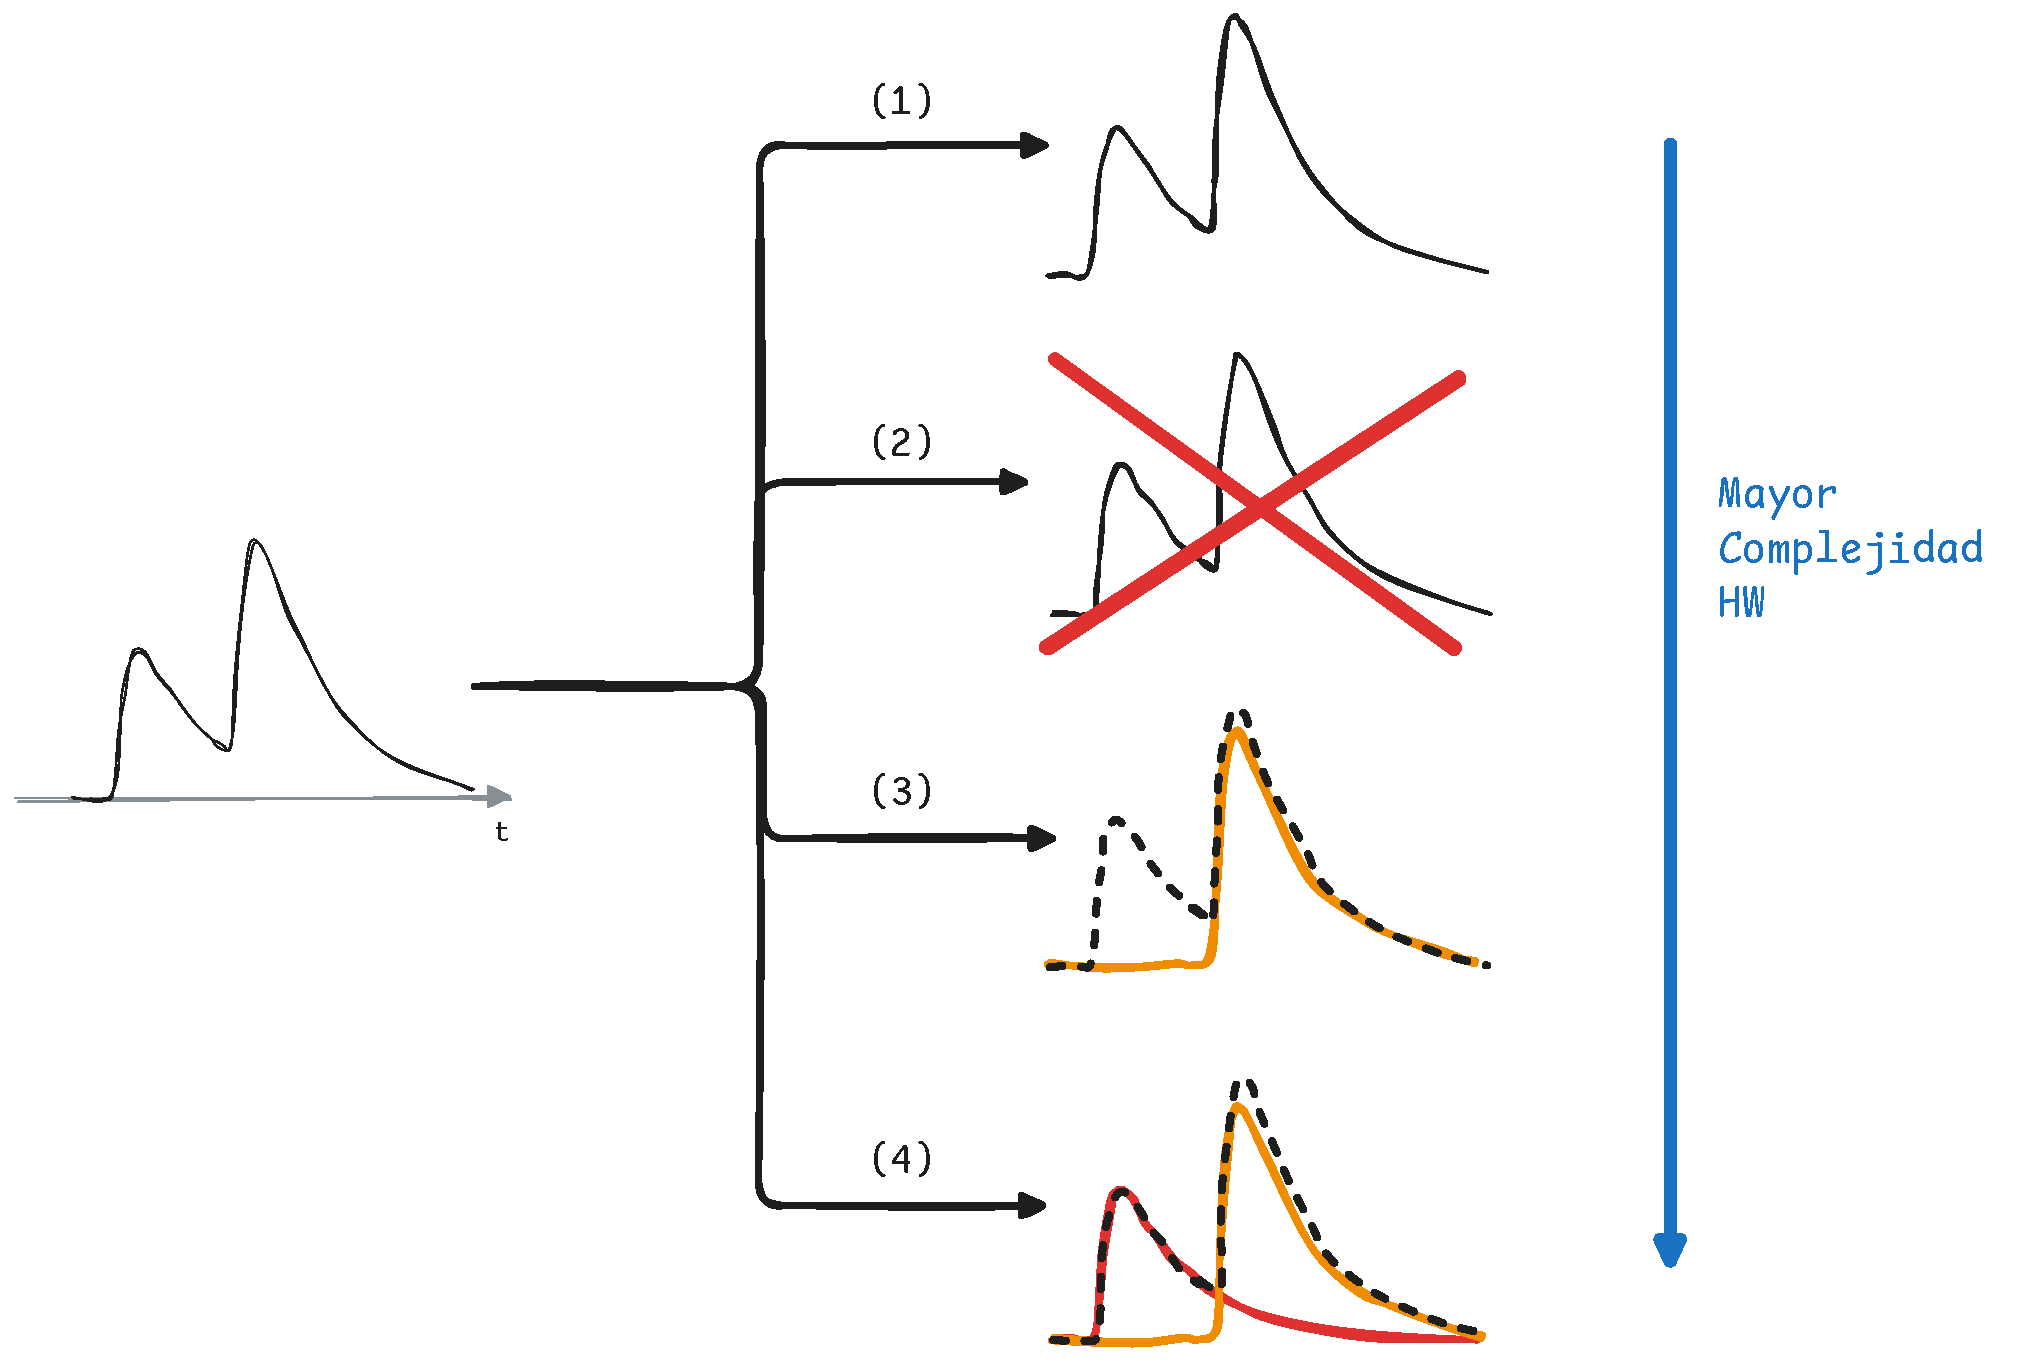
\includegraphics{cap1_metodos_recuperacion}
\caption[Formas de tratar un evento apilado]{%
Las cuatro formas de tratar un evento apilado, ordenadas de menor a mayor
complejidad de HW.\label{f:mca-metodos-recuperacion}}
\end{figure}

La opción de descarte (2) puede ser más que suficiente si los pulsos son
\textbf{independientes en el tiempo}. En ese caso tenemos una reducción en la
cantidad de eventos medidos (y, en consecuencia, en la significancia
estadística), que se resuelve fácilmente aumentando el tiempo de medición.

Esta opción falla cuando los pulsos están \textbf{correlacionados en el tiempo}:
el segundo pulso no llega al azar sino como consecuencia del primero, y
descartar los eventos apilados elimina justamente los de interés. Por ejemplo,
en un detector Cherenkov de agua (\emph{water-Cherenkov
detector})~\cite{Allison2005}, un muón que atraviesa el volumen emite fotones
por efecto Cherenkov a lo largo de su trayectoria. Si el muón se frena y se
detiene dentro del detector, decae en un electrón con una vida media de
$\approx$\qty{2.2}{\micro\second}~\cite{PDG2024}, y el electrón produce un
segundo pulso. Los dos pulsos están correlacionados: su separación sigue una
exponencial de $\approx$\qty{2.2}{\micro\second}, del orden del ancho de los
pulsos conformados, de modo que muchos de esos pares aparecen apilados.

En estos casos conviene rescatar los pulsos, con la tercera o la cuarta opción,
que tienen un criterio de corrección:
\begin{itemize}
  \item La tercera necesita una prioridad para decidir qué pulso rescata, pero
    tiene la ventaja de que \textbf{cada evento se asocia con un único cálculo
    de estadístico}, por lo que es más simple de implementar.
  \item La cuarta requiere poder procesar múltiples pulsos por evento.
    \textbf{Requiere implementar una cola de procesamiento dentro del sistema};
    los detalles se encuentran en la
    Sec.~\refpend{S:implmca-recuperacion}{Implementación del MCA: métodos de
    recuperación del pulso}.
\end{itemize}

\subsection{\texorpdfstring{\emph{Amplitude walk}}{Amplitude walk}}
\label{S:mca-amplitude-walk}

Es la \textbf{diferencia temporal en el disparo} de eventos de una misma familia
de pulsos debida a la diferencia en su amplitud máxima~\cite{Knoll2010}. En la
Fig.~\ref{f:mca-amplitude-walk} se presentan tres pulsos de la misma forma, con
igual tiempo de subida $t_s$ y de bajada $t_b$, que llegan exactamente al mismo
tiempo pero tienen distinta amplitud.

\begin{figure}[H]
\centering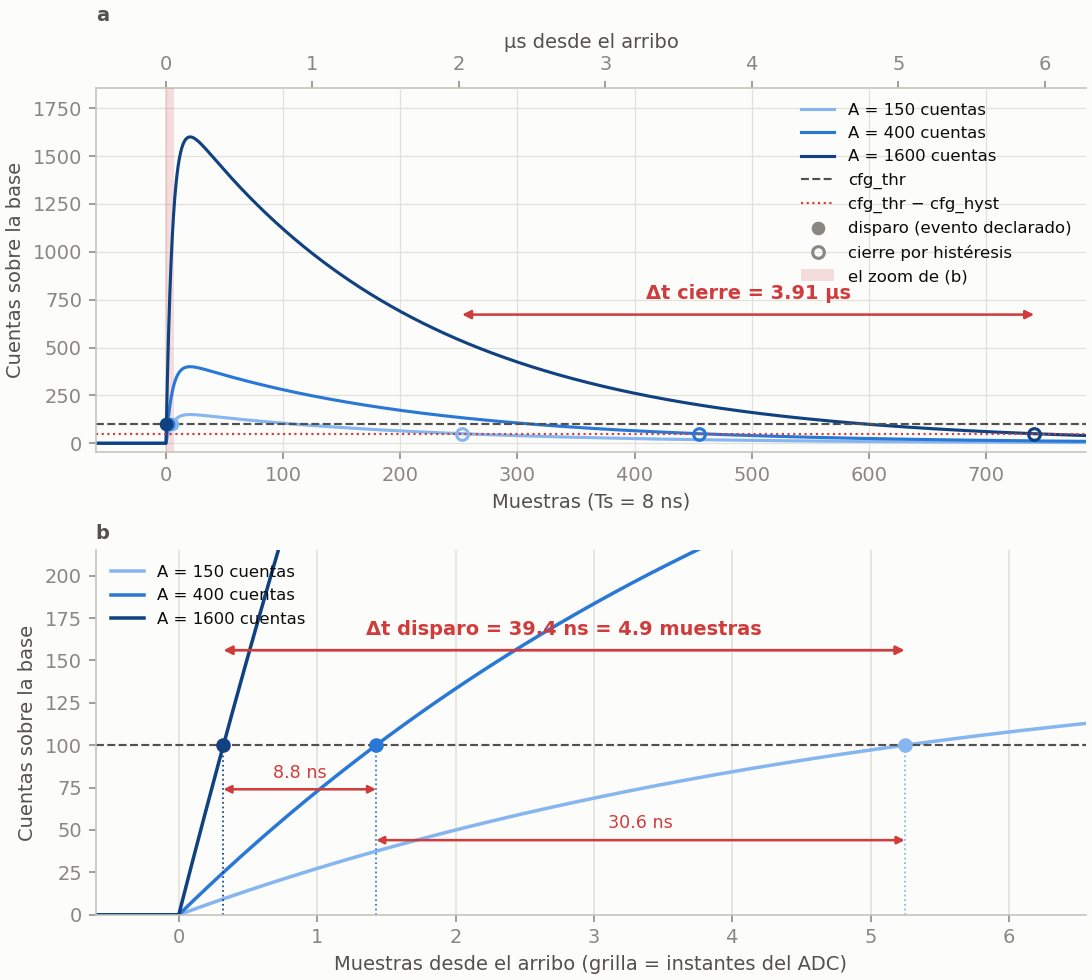
\includegraphics{cap1_amplitude_walk}
\caption[\emph{Amplitude walk} para tres pulsos de la misma familia]{%
(a) \emph{Amplitude walk} para tres pulsos de la misma familia que llegan a la
vez, con el disparo y el cierre por histéresis de cada uno. (b) Detalle de la
diferencia temporal de disparo entre los tres pulsos.\label{f:mca-amplitude-walk}}
\end{figure}

Sin embargo, la detección del pulso de 1600~ADU ocurre \qty{8.8}{\nano\second}
antes que la del de 400~ADU, y \qty{39.4}{\nano\second} antes que la del de
150~ADU: el pulso más grande cruza el umbral primero porque sube más rápido.

De esta forma tenemos una distribución de largos de la \textbf{ventana de tiempo
previa al disparo}: la porción de la subida que queda antes del disparo depende
de la amplitud. Generalmente nos importa su valor máximo, que corresponde a los
pulsos más chicos. Según el conformado esto puede no ser un problema; es peor
para conformados con tiempos de subida lentos, especialmente para el CR-RC$^4$.
El walk también corre el cierre por histéresis, y mucho más, porque ese cruce
ocurre sobre la cola exponencial: en la Fig.~\ref{f:mca-amplitude-walk}(a) los
cierres de los tres pulsos se separan \qty{3.91}{\micro\second}.

En nuestra implementación se decidió que la ventana de tiempo previa al disparo
sea fija: la señal se retrasa una cantidad configurable de ciclos antes de
entrar a la ventana, de modo que el pie del pulso ya esté adentro cuando llega
el disparo. Para la altura máxima es una buena decisión, porque la subida no se
descarta y el ápice queda siempre dentro de la ventana. Para los estadísticos
que integran la subida, como la carga o el factor de forma, la porción de la
ventana previa que cae antes del pie del pulso depende de la amplitud: si no se
resta la línea de base, esa porción suma a la carga un término que varía con la
amplitud, y si el retardo no alcanza a cubrir el walk de los pulsos más chicos,
a ellos se les pierde parte de la subida. En ambos casos es una no linealidad
concentrada cerca del umbral, y por eso estos estadísticos se calculan sobre la
señal con la línea de base restada (ver
Sec.~\refpend{S:implmca-linea-base}{Implementación del MCA: recuperación de
línea de base}).

%%%%%%%%%%%%%%%%%%%%%%%%%%%%%%%%%%%%%%%%%%%%%%%%%%%%%%%%%%%%%%%%%%%%%%%%%%%%%%%%
\section{Tiempo muerto y tiempo vivo}
\label{S:mca-tiempo-muerto}

Inicialmente definimos el tiempo muerto como \textbf{el tiempo en el cual el
sistema no puede procesar un nuevo evento de la forma deseada}; el tiempo vivo
es su complemento. Sus causas incluyen limitaciones en cada una de las secciones
del sistema. Reducirlo es la razón principal de la existencia del MCA: como
procesa cada evento en el hardware y solo transfiere el histograma, su tiempo
muerto es un orden de magnitud menor que el de la captura de trazas con el
módulo de osciloscopio (OSC). En la Sec.~\ref{S:intro-hw-back-pressure}
describimos cómo \textbf{medir} y diseñar un sistema para reducir al máximo el
tiempo muerto de medición.

\subsection{Modelos fundamentales de tiempo muerto}
\label{S:mca-modelos-tiempo-muerto}

Por el tiempo muerto, la tasa registrada $m$ es menor que la tasa real de
eventos $n$. Para corregirla necesitamos un modelo que vincule ambas, y todo
modelo depende del tiempo muerto $\tau$. En esta sección presentamos los dos
modelos más sencillos y mostramos por qué \textbf{necesitamos determinar $\tau$
con precisión}: la corrección amplifica cualquier error en $\tau$, y la
amplificación crece con la tasa.

Ambos modelos describen el comportamiento del sistema frente a eventos
sucesivos separados un tiempo $\Delta T$. Uno se denomina
\textbf{paralizable}, porque cada vez que llega un evento la ventana de tiempo
muerto se reinicia, aunque ese evento no se registre. En el \textbf{no
paralizable}, en cambio, la ventana de tiempo muerto no se reinicia por la
llegada de nuevos eventos: lo que llega durante ella se pierde sin extenderla.
En la Fig.~\ref{f:mca-tren-rho05} se presenta el mismo tren de arribos para
ambos modelos.

\begin{figure}[H]
\centering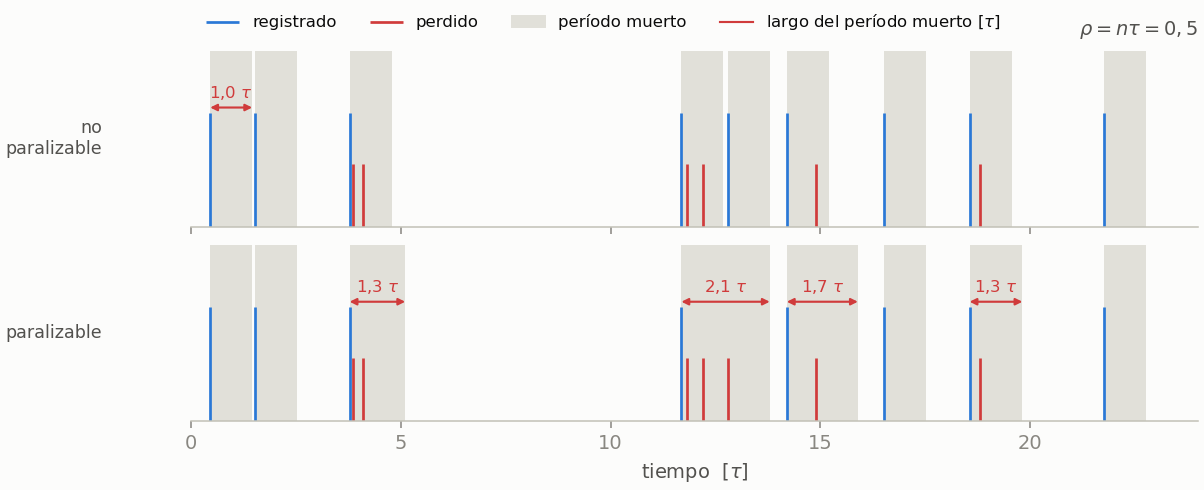
\includegraphics{cap1_tren_rho05}
\caption[Un tren de arribos de Poisson visto por los dos modelos de tiempo
muerto]{%
Un mismo tren de arribos de Poisson con $\rho = n\tau = 0.5$ visto por los dos
modelos. En el no paralizable cada período muerto dura $\tau$; en el
paralizable los arribos perdidos lo extienden.\label{f:mca-tren-rho05}}
\end{figure}

Para cada uno de estos modelos podemos calcular los parámetros importantes, como
la fracción de tiempo vivo, la fracción de eventos aceptados, el largo promedio
de la ventana muerta y, el más importante de todos, la \textbf{tasa registrada
en función de la tasa incidente}. En la Tabla~\ref{t:mca-tiempo-muerto} se
presentan las relaciones fundamentales de los dos modelos para arribos de
Poisson; su deducción se encuentra en Knoll~\citecap{Knoll2010}{4}, y una
revisión de sus variantes, en Müller~\cite{Muller1973}.

\begin{table}[H]
\centering
\caption[Modelos de tiempo muerto no paralizable y paralizable]{%
Relaciones fundamentales de los modelos no paralizable y paralizable para
arribos de Poisson de tasa $n$; $W$ es la función de
Lambert~\cite{Corless1996}.\label{t:mca-tiempo-muerto}}
\renewcommand{\arraystretch}{2.1}
\begin{tabular}{|l|c|c|}
\hline
\encabezado & \textbf{No paralizable} (tipo I) & \textbf{Paralizable} (tipo II) \\ \hline
Tasa registrada           & $m = \dfrac{n}{1+n\tau}$
                          & $m = n\,e^{-n\tau}$ \\ \hline
Tasa real despejada       & $\hat n = \dfrac{m}{1-m\tau}$
                          & $\hat n = -\dfrac{W(-m\tau)}{\tau}$ \\ \hline
Fracción perdida          & $1-\dfrac{m}{n} = \dfrac{n\tau}{1+n\tau}$
                          & $1-\dfrac{m}{n} = 1-e^{-n\tau}$ \\ \hline
Fracción de tiempo muerto & $m\tau = \dfrac{n\tau}{1+n\tau}$
                          & $1-e^{-n\tau}$ \\ \hline
Límite $n\tau\ll 1$       & $m \simeq n\,(1-n\tau)$
                          & $m \simeq n\,(1-n\tau)$ \\ \hline
Límite $n\to\infty$       & $m \to 1/\tau$
                          & $m \to 0$ \\ \hline
Máximo                    & no tiene, es monótona
                          & $m_{\max} = \dfrac{1}{e\,\tau}$ en $n = 1/\tau$ \\ \hline
\end{tabular}
\end{table}

En la Fig.~\ref{f:mca-tasa-registrada} representamos la \textbf{tasa medida
normalizada} $m\tau$ \textbf{en función de la tasa incidente normalizada}
$n\tau$, en el estado estacionario, para ambos modelos. El producto
$\rho = n\tau$ es la cantidad promedio de eventos incidentes durante una ventana
de tiempo muerto, y es el único parámetro del que dependen las curvas. A tasas
bajas, $n\tau \ll 1$, los dos modelos coinciden y $m \simeq n$. A medida que
$n\tau$ se acerca a 1 se separan, y en $n\tau = 1$ ya se registra a lo sumo la
mitad de los eventos ($m\tau = 1/2$ en el no paralizable y
$m\tau = 1/e \approx 0.37$ en el paralizable).

\begin{figure}[H]
\centering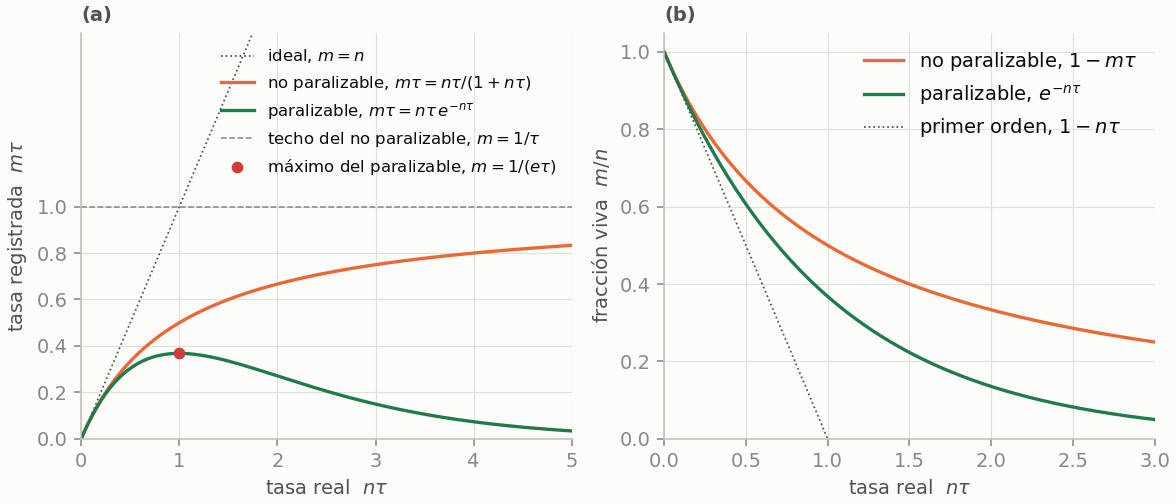
\includegraphics{cap1_tasa_registrada}
\caption[Tasa registrada contra tasa incidente]{%
(a) Tasa registrada contra tasa incidente, ambas normalizadas por $\tau$, para
los dos modelos y la diagonal ideal. (b) La fracción de tiempo vivo de la que
salen las dos fórmulas.\label{f:mca-tasa-registrada}}
\end{figure}

La implicancia es doble. Por un lado, la \textbf{cantidad de cuentas medidas en
un tiempo $T$ no es lineal con la tasa incidente}:
\begin{equation}
  N_T = m\,T = \frac{n\,T}{1+n\tau}\quad\text{(no paralizable)},\qquad
  N_T = n\,T\,e^{-n\tau}\quad\text{(paralizable)}
  \label{e:mca-cuentas}
\end{equation}
En el caso paralizable la relación ni siquiera es monótona: $N_T$ alcanza un
máximo $T/(e\tau)$ en $n = 1/\tau$ y decrece después, de modo que aumentar la
actividad de la fuente \textbf{reduce} la estadística disponible.

Por otro lado, la tasa real no se mide: se \textbf{estima} invirtiendo el
modelo, $\hat n(m, \tau)$, y esa estimación hereda los errores de las dos
magnitudes que entran en ella. El error en la tasa medida $m$ es estadístico y
se reduce midiendo más tiempo; el error en $\tau$ depende de qué tan bien
conozcamos el sistema. Para ver cuánto pesa cada uno propagamos a primer orden:
\begin{equation}
  \delta \hat n = \frac{\partial \hat n}{\partial m}\,\delta m
                + \frac{\partial \hat n}{\partial \tau}\,\delta \tau
  \label{e:mca-propagacion}
\end{equation}
En el caso no paralizable la estimación es explícita, $\hat n = m/(1-m\tau)$, y
las dos derivadas parciales, los \textbf{coeficientes de
sensibilidad}~\cite{GUM2008} de la medición, se calculan de forma directa:
\begin{equation}
  \frac{\partial \hat n}{\partial m} = \frac{1}{(1-m\tau)^2}, \qquad
  \frac{\partial \hat n}{\partial \tau} = \frac{m^2}{(1-m\tau)^2}
  \label{e:mca-sensibilidad-np}
\end{equation}
Pasamos a errores relativos, que son los que entrega la estadística de conteo y
los que tiene sentido reportar, dividiendo por $\hat n$ y usando
$n\tau = m\tau/(1-m\tau)$:
\begin{equation}
  \begin{split}
  \frac{\delta \hat n}{\hat n}
    &= \frac{1}{1-m\tau}\,\frac{\delta m}{m}
     + \frac{m\tau}{1-m\tau}\,\frac{\delta \tau}{\tau} \\
    &= (1+n\tau)\,\frac{\delta m}{m} + n\tau\,\frac{\delta \tau}{\tau}
  \end{split}
  \label{e:mca-relativo-np}
\end{equation}
Los dos coeficientes difieren exactamente en una unidad.

El caso paralizable no admite un despeje elemental, pero tampoco lo necesita:
basta con diferenciar el modelo directo $m = n\,e^{-n\tau}$ de forma implícita y
usar $e^{n\tau} = n/m$ para simplificar el primer término:
\begin{equation}
  \begin{gathered}
  \delta m = e^{-n\tau}\Big[(1-n\tau)\,\delta n - n^2\,\delta \tau\Big] \\
  \Longrightarrow\qquad
  \frac{\delta n}{n} = \frac{1}{1-n\tau}\,\frac{\delta m}{m}
                     + \frac{n\tau}{1-n\tau}\,\frac{\delta \tau}{\tau}
  \end{gathered}
  \label{e:mca-relativo-p}
\end{equation}
De nuevo, los dos coeficientes difieren en una unidad.

No es una coincidencia. Escrita en las cantidades adimensionales $m\tau$ y
$n\tau$, toda calibración es una función $n\tau = g(m\tau)$ sin parámetros
libres, y la estimación es $\hat n = g(m\tau)/\tau$. Aplicando la regla del
producto y normalizando cada coeficiente de sensibilidad:
\begin{equation}
  \begin{gathered}
  \frac{m}{\hat n}\frac{\partial \hat n}{\partial m}
    = \frac{m\tau\,g'(m\tau)}{g(m\tau)} \equiv E, \\
  \frac{\tau}{\hat n}\frac{\partial \hat n}{\partial \tau}
    = \frac{m\tau\,g'(m\tau)}{g(m\tau)} - 1 = E-1
  \end{gathered}
  \label{e:mca-E}
\end{equation}
Llamamos a $E$ el \textbf{término de amplificación de error}. Es la pendiente de
la curva de calibración en escala logarítmica,
$E = d\ln(n\tau)/d\ln(m\tau)$: la corrección amplifica los errores exactamente
en la medida en que esa curva se aplana. Como $m$ y $\tau$ son magnitudes
independientes, sus contribuciones se combinan en cuadratura según la ley de
propagación de incertidumbres~\cite{GUM2008}:
\begin{equation}
  \left(\frac{\delta \hat n}{\hat n}\right)^{2}
    = E^{2}\left(\frac{\delta m}{m}\right)^{2}
    + (E-1)^{2}\left(\frac{\delta \tau}{\tau}\right)^{2}
  \label{e:mca-cuadratura}
\end{equation}
con
\begin{equation}
  E = \frac{1}{1-m\tau} = 1+n\tau \quad\text{(no paralizable)}, \qquad
  E = \frac{1}{1-n\tau} \quad\text{(paralizable)}
  \label{e:mca-E-modelos}
\end{equation}

El coeficiente que pesa el error en $\tau$, $E-1$, es el que motiva esta
sección. Vale $n\tau$ en el modelo no paralizable y $n\tau/(1-n\tau)$ en el
paralizable: se anula a tasa baja, donde la corrección misma es chica, y crece
con la tasa. A $n\tau = 0.5$, un error del \qty{1}{\percent} en $\tau$ se
convierte en un error de \qty{0.5}{\percent} en la tasa corregida en el modelo
no paralizable y de \qty{1}{\percent} en el paralizable; a $n\tau = 0.9$, en
\qty{0.9}{\percent} y \qty{9}{\percent}, respectivamente. Además, este error es
\textbf{sistemático}: a diferencia del de $m$, no se reduce aumentando el tiempo
de medición. La incerteza en $\tau$ fija entonces un piso a la exactitud de la
tasa corregida y, con él, la tasa máxima a la que podemos trabajar con una
exactitud dada. Por eso \textbf{necesitamos determinar $\tau$ con precisión}, y
no tomarlo de un valor nominal: un $\tau$ mal determinado produce variaciones
grandes en las tasas corregidas, justamente en el régimen de tasas altas, que es
donde la corrección más importa.

Si graficamos ambos coeficientes obtenemos la
Fig.~\ref{f:mca-amplificacion}: el panel (a) muestra $E$, el factor que pesa el
error en la tasa medida, y el (b) muestra $E-1$, el que pesa el error en el
tiempo muerto, ambos contra $\rho = n\tau$. En el modelo no paralizable la
pendiente de la calibración decae suavemente y $E$ crece de forma lineal con la
tasa. En el paralizable la calibración se vuelve horizontal en $\rho = 1$ y $E$
diverge, porque allí ningún valor medido distingue tasas incidentes vecinas.
Para $\rho > 1$ el coeficiente del modelo paralizable cambia de signo, porque se
está en la rama descendente de la curva; la figura grafica su valor absoluto,
así que su caída pasado $\rho = 1$ no indica que la corrección mejore.

\begin{figure}[H]
\centering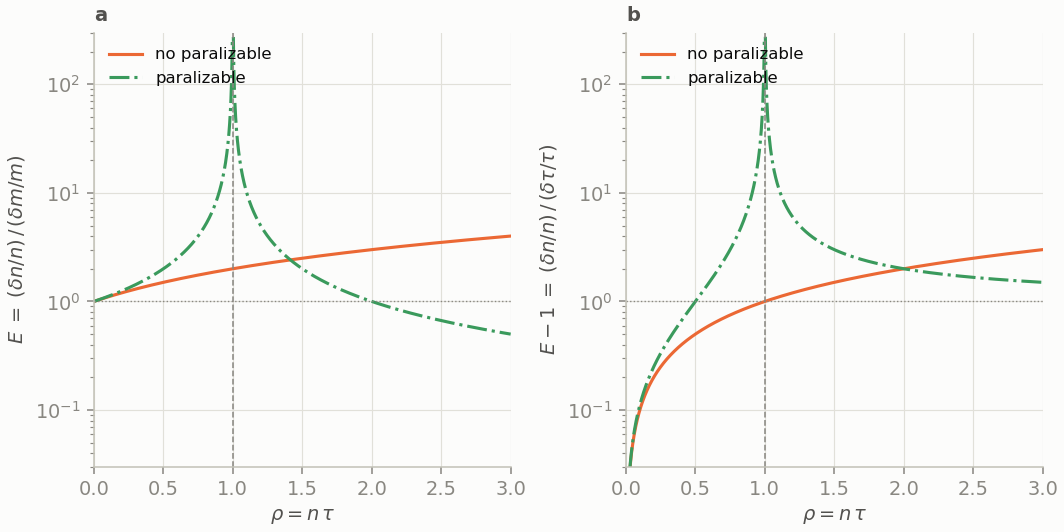
\includegraphics{cap1_amplificacion_correccion}
\caption[Amplificación de error de la corrección de tasa]{%
Amplificación de error de la corrección de tasa en función de $\rho = n\tau$:
(a) $E$, que pesa el error relativo de la tasa medida; (b) $E-1$, que pesa el
error relativo del tiempo muerto.\label{f:mca-amplificacion}}
\end{figure}

Para la versión paralizable hay además un problema cualitativo: al no ser
monótona, a una misma tasa medida le corresponden \textbf{dos} tasas incidentes
posibles, una a cada lado de $n = 1/\tau$. Sin una idea previa del rango de
tasas o alguna medición auxiliar, no es posible decidir cuál de las dos
correcciones es la correcta.

\begin{destacado}
Es así que nos propusimos que nuestro sistema tenga la capacidad de
\textbf{reportar la distribución del tiempo muerto} y la cantidad de
\textbf{eventos rechazados}, de modo de medir el tiempo muerto en cada
adquisición en lugar de suponerlo, y de poder analizar posteriormente qué tan
válidos son los resultados obtenidos y cuál de los dos modelos aplica a nuestro
sistema.
\end{destacado}

Esto es necesario porque cuál de los modelos aplica mejor \textbf{depende de los
parámetros elegidos}. En la Fig.~\ref{f:mca-politicas-final}(b), por ejemplo, la
llegada de nuevos pulsos alarga la ventana, porque esta termina recién cuando la
señal decae hasta el nivel de relajación: es un comportamiento paralizable. Lo
mismo ocurre con la ventana fija de (a), porque el disparador por nivel no se
re-arma mientras la cola siga por encima del umbral, y cada pulso que llega en
ese lapso la mantiene arriba.

Un caso típico en el que ninguno de los dos modelos aplica es el ensayo con una
fuente periódica de laboratorio, como un generador de pulsos, en la que la
separación entre pulsos es constante. Si el período es mayor que $\tau$, cada
pulso encuentra al sistema libre y no se pierde ninguno; con arribos de Poisson,
en cambio, se pierde una fracción $\approx n\tau$ a cualquier tasa, porque los
arribos se agrupan. Una eficiencia medida con un generador periódico es una
propiedad del estímulo y no del equipo, y no puede trasladarse a una fuente
radiactiva. Por eso, para caracterizar el tiempo muerto usamos también trenes
de pulsos con arribos de Poisson.

%%%%%%%%%%%%%%%%%%%%%%%%%%%%%%%%%%%%%%%%%%%%%%%%%%%%%%%%%%%%%%%%%%%%%%%%%%%%%%%%
\section{Características de mérito del sistema}
\label{S:mca-merito}

Con estas caracterizamos la desviación, RMS o máxima, de la respuesta del
sistema respecto de la esperada. La caracterización experimental consiste en
inyectar una secuencia de pulsos conocida y analizar la distribución obtenida.
En la Fig.~\ref{f:mca-merito} se presentan los tres parámetros más importantes
(Knoll~\citecap{Knoll2010}{18}): la resolución FWHM, la no linealidad integral
(INL) y la no linealidad diferencial (DNL). Las tres son independientes y
arruinan cosas distintas: la INL corre el pico, la DNL lo deforma y la
resolución finita lo ensancha.

\begin{figure}[H]
\centering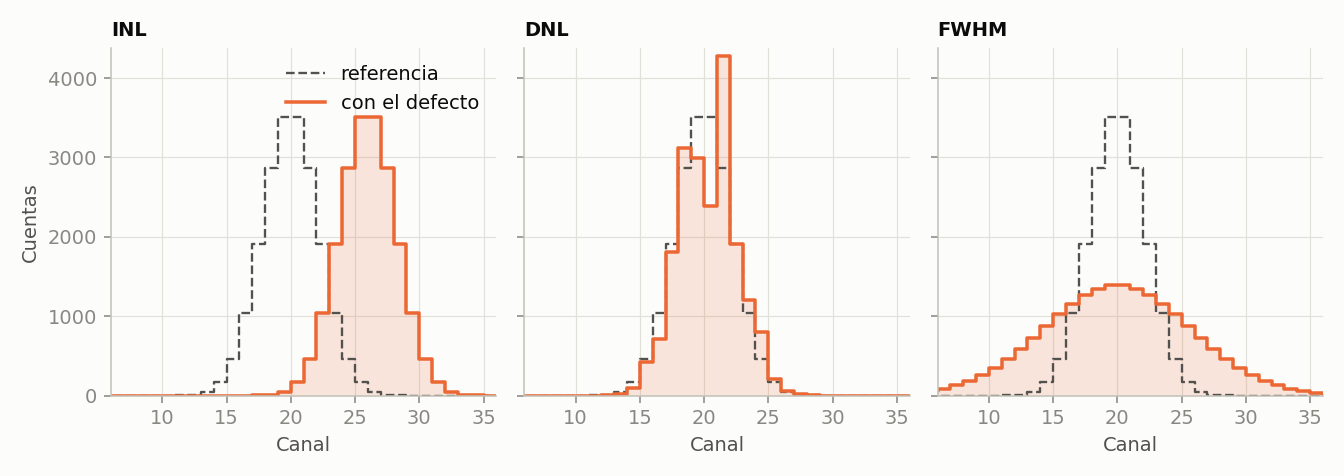
\includegraphics{cap1_tres_metricas}
\caption[Figuras de mérito de un MCA: FWHM, INL y DNL]{%
El mismo pico de referencia (línea de trazos) visto con cada defecto por
separado. Datos sintéticos.\label{f:mca-merito}}
\end{figure}

\subsection{Resolución FWHM}
\label{S:mca-fwhm}

Es el \textbf{ancho del pico a media altura}, de ahí su nombre: \emph{full width
at half maximum} (FWHM). Normalmente se lo expresa como porcentaje de la altura
de su centroide $H_0$, $R = \mathrm{FWHM}/H_0$. Pulsos idénticos caerían todos
en un mismo canal, así que el ancho que se mide es ensanchamiento: ruido de la
cadena, cuantización y jitter del estimador de amplitud. Es el piso del sistema
y la única de las tres métricas que no se compensa por software, porque el
ensanchamiento es aleatorio. Cuando el pico se ensancha, dos líneas cercanas
dejan de separarse.

\subsection{No linealidad integral (INL)}
\label{S:mca-inl}

El amplificador ideal consiste en una ganancia lineal $G$, de forma que la
amplitud medida ideal sería $\hat A_\text{ideal} = G A$. Las no idealidades
generalmente se tienen en cuenta con dos parámetros: el offset del cero $A_0$ y
el residuo a lo largo de la curva de amplificación,
\begin{equation}
  \hat A = G \cdot (A-A_0) + \text{INL}(A-A_0)
  \label{e:mca-inl}
\end{equation}
La INL mide cuánto se aparta la relación real entre amplitud y canal de la
\textbf{recta ideal}~\cite{IEEE1241}. Es una función $\text{INL}(A)$, pero
normalmente se la describe por su valor máximo,
$\text{INL} = \max_A |\text{INL}(A)|$.

En el panel INL de la Fig.~\ref{f:mca-merito} se representa un ejemplo con
$A_0 = 0$, en el que la expresión se simplifica a
$\hat A = G \cdot A + \text{INL}(A)$: la forma del pico queda intacta, pero el
pico está donde no va. En la práctica se ajusta una recta a los centroides
medidos para varias amplitudes, y el residuo del ajuste es $\text{INL}(A)$. Se
la calcula con la siguiente expresión
\begin{equation}
  \text{INL} = \frac{\max|\text{residuo}|}{\text{canal}_{\max} - \text{canal}_{\min}}
  \label{e:mca-inl-max}
\end{equation}
y generalmente se la expresa en porcentaje del rango barrido o del fondo de
escala. Como es un error sistemático, la INL se puede compensar con una
calibración. La curva medida en nuestro sistema se presenta en la
Sec.~\ref{S:res-inl-trapecio}.

\subsection{No linealidad diferencial (DNL)}
\label{S:mca-dnl}

Es la \textbf{variación} del \textbf{ancho de cada canal respecto del
promedio}~\cite{IEEE1241},
$\text{DNL}_i = \Delta H_i / \overline{\Delta H} - 1$. Se mide llenando el
espectro con amplitudes uniformemente distribuidas, por ejemplo con un
generador de amplitud deslizante: si todos los canales fueran iguales recibirían
la misma cantidad de cuentas, así que la desviación relativa de las cuentas
\emph{es} la DNL.

Un canal más ancho junta más cuentas y \textbf{crea estructura que no está en la
señal}: deforma los picos, sesga el área y el centroide, y en el peor caso
genera picos falsos. Cuando es periódica (típico de los ADC, en las transiciones
de bits) produce un rizado regular en todo el espectro.

\subsection{Resolución de par de pulsos}
\label{S:mca-par-pulsos}

Es la capacidad de un sistema de \textbf{disparo} de distinguir dos pulsos
superpuestos separados un tiempo $\Delta t$ variable; se la caracteriza con la
menor separación a la que el sistema dispara dos veces. Una propiedad distinta
es la capacidad de recuperar los estadísticos de los pulsos originales a partir
de su superposición; para ello se refiere a la
Sec.~\refpend{S:implmca-linea-base}{Implementación del MCA: recuperación de
línea de base}.

\subsection{Selección del tipo de bineado}
\label{S:mca-bineado}

Podemos configurar el módulo de forma que el indexado de la memoria de
acumulación tenga \textbf{dos índices en lugar de uno solo}, con lo que el
histograma medido se vuelve 2D. Esto nos da dos opciones:
\begin{enumerate}
  \item Histograma 1D de $2^N$ divisiones.
  \item Histograma 2D de $2^{N_1} \times 2^{N_2}$ divisiones.
\end{enumerate}

Como empleamos división uniforme en ambos casos, la demanda de memoria en el
caso 2D escala con el producto de las divisiones, $2^{N_1+N_2}$. Con la misma
memoria que un histograma 1D de $2^N$ canales, el 2D reparte los bits entre los
dos ejes, $N_1 + N_2 = N$, y cada eje queda con mucha menos resolución.

Algunas aplicaciones del MCA 2D \emph{intracanal}, es decir, en el que ambas
\textbf{features son del mismo evento}, se presentan en el
Apéndice~\ref{S:ap-mca2d}. En la Fig.~\ref{f:mca-2d} se presenta un ejemplo de
histograma de dos variables para la \textbf{identificación
$\alpha/\beta/\gamma$}, en el que se grafica la altura máxima contra un factor
de forma del pulso para separar las partículas $\alpha$ de las $\beta/\gamma$.

\begin{figure}[H]
\centering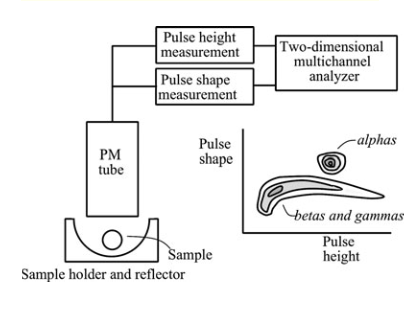
\includegraphics[width=0.6\linewidth]{cap1_mca2d_knoll}
\caption[Identificación $\alpha/\beta/\gamma$ con un histograma de dos
variables]{%
Identificación $\alpha/\beta/\gamma$ con un histograma de dos variables.
Extraída de Knoll~\cite{Knoll2010}.\label{f:mca-2d}}
\end{figure}

Existen también MCA 2D cuyos ejes trabajan sobre \textbf{eventos de diferentes
canales}. En particular, permiten un análisis de coincidencias y
anticoincidencias~\cite{Knoll2010}, en el que el disparo de un evento requiere
varias condiciones mutuas. El caso más sencillo es la coincidencia: que dos
canales disparen dentro de una ventana de tiempo $\Delta T$ dada. En la
anticoincidencia, en cambio, se requiere que un canal en particular dispare y
que otro \textbf{no} lo haga dentro de la ventana.

% Bibliografía de este capítulo. Va al final del archivo, siempre.
\bibliografiacapitulo

%%% Local Variables:
%%% mode: latex
%%% TeX-master: "template"
%%% End:
      % Analizador multicanal
% Origen: Secciones/PI - Hardware empleado.md
\chapter{Hardware empleado}
\label{C:hw}

% Figuras de ESTE capítulo + las compartidas. Siempre al principio del archivo.
\graphicspath{{figs/cap2/}{figs/comunes/}}

\begin{destacado}
En este capítulo se describe (1) por qué necesitamos un módulo de aceleración de
hardware en vez de un microcontrolador, (2) qué plataformas de hardware
programable existen, (3) la plataforma empleada, la Red Pitaya STEMlab 125-14, y
la arquitectura de su SoC Zynq-7000, y (4) los periféricos de la placa.
\end{destacado}

%%%%%%%%%%%%%%%%%%%%%%%%%%%%%%%%%%%%%%%%%%%%%%%%%%%%%%%%%%%%%%%%%%%%%%%%%%%%%%%%
\section{Por qué un módulo de aceleración de HW en vez de un microcontrolador}
\label{S:hw-por-que-acelerador}

La respuesta tiene múltiples razones; los dos factores decisivos son la
\textbf{tasa de muestreo} y la \textbf{capacidad de procesamiento}. Partimos del
criterio de diseño: ``el dispositivo debe ser capaz de \textbf{recuperar} pulsos
con flancos del orden de los $\sim 100\,\text{ns}$''. Si deseamos más de 10
muestras en el flanco del pulso (\emph{samples per pulse}, $\text{spp}>10$), hay
que muestrear a $10/100\,\text{ns} = 100$~MSPS o más para resolver su forma.

\begin{table}[H]
\centering
\caption[Tasas de muestreo de los ADC de distintas plataformas]{%
Comparación de las tasas de muestreo de los ADC de distintas
plataformas~\cite{STM32H723,STM32F407}.\label{t:hw-tasas}}
\small
\begin{tabularx}{\textwidth}{|>{\raggedright\arraybackslash}X|c|>{\centering\arraybackslash}p{0.2\textwidth}|>{\centering\arraybackslash}p{0.2\textwidth}|}
\hline
\encabezado \textbf{Tasa de muestreo} & \textbf{Período}
  & \textbf{Muestras en el flanco de 100~ns} & \textbf{Muestras en un pulso de 300~ns} \\ \hline
\textbf{125 MSPS} (Red Pitaya) & 8~ns & \textbf{$\sim$12} & \textbf{$\sim$37} \\ \hline
5 MSPS (ADC de 12 bits del STM32H723/733) & 200~ns & 0,5 & 1,5 \\ \hline
3,6 MSPS (ADC de 16 bits del STM32H7) & 278~ns & 0,36 & $\sim$1 \\ \hline
2,4 MSPS (STM32F407) & 417~ns & 0,24 & 0,72 \\ \hline
\end{tabularx}
\end{table}

Ni siquiera entrelazando los tres ADC del STM32F407 (7,2~MSPS) se llega a una
muestra por flanco. Por eso los analizadores multicanal basados en µC recurren a
un conformado analógico con tiempos del orden de los microsegundos y a
detectores de pico~\cite{Knoll2010}: circuitos analógicos que retienen el valor
pico (o la carga) hasta una operación de descarga. Esto renuncia a medir la forma
del pulso, pero es la solución adecuada si el spp es bajo. Si en cambio
analizamos la \textbf{cantidad de ciclos de reloj disponibles por muestra},
obtenemos lo presentado en la Tabla~\ref{t:hw-plataformas}.

\begin{table}[H]
\centering
\caption[Comparación de plataformas: reloj, ciclos por muestra y ADC]{%
Comparación de plataformas: reloj, ciclos de reloj disponibles por muestra si la
entrada fuera de 125~MSPS, ADC integrado y tasas típicas de
trabajo~\cite{STM32F407,STM32H723,TMS320F2837xD,RedPitayaDocs}.
\label{t:hw-plataformas}}
\footnotesize
\setlength{\tabcolsep}{3pt}
\newcolumntype{Y}{>{\raggedright\arraybackslash}X}
\begin{tabularx}{\textwidth}{|>{\raggedright\arraybackslash}p{0.17\textwidth}|>{\raggedright\arraybackslash}p{0.1\textwidth}|>{\raggedright\arraybackslash}p{0.11\textwidth}|Y|Y|Y|}
\hline
\encabezado \textbf{Plataforma} & \textbf{Tipo} & \textbf{Reloj}
  & \textbf{Ciclos por muestra (a 125~MSPS)} & \textbf{ADC}
  & \textbf{Tasas típicas de trabajo} \\ \hline
\textbf{Cortex-M4F} (STM32F407) & µC & 168~MHz & 1,3
  & integrado: 12 bits, 2,4~MSPS (7,2~MSPS entrelazando 3 ADC)
  & audio de 48--192~kHz; MCA con detector de pico analógico \\ \hline
\textbf{Cortex-M7} (STM32H723/733) & µC & 480~MHz & 3,8
  & integrado: 16 bits a 3,6~MSPS; 12 bits a 5~MSPS
  & MCA digital a 3,6~MSPS con pulsos de µs \\ \hline
\textbf{TI C2000} (F28379D) & µC (DSC) & 200~MHz, 800~MIPS
  & 1,6 por núcleo (6,4 instrucciones sumando 2 núcleos y 2 CLA)
  & integrado: 16 bits a 1,1~MSPS; 12 bits a 3,5~MSPS
  & lazos de control de 10--100~kHz \\ \hline
\textbf{Red Pitaya STEMlab 125-14} & SoC: FPGA + 2~$\times$ Cortex-A9
  & 125~MHz (PL) · 667~MHz (PS)
  & PL: 1, pero en cada ciclo ejecuta todas las etapas a la vez · PS: 5,3 por
    núcleo
  & externo: LTC2145, 14 bits, 125~MSPS
  & \textbf{125~MSPS sostenidos, 2 canales} \\ \hline
\end{tabularx}
\end{table}

Si suponemos que cada canal de muestreo dispone de todo el tiempo de ejecución,
podemos estimar las operaciones que requiere cada muestra; la suma aproximada se
presenta en la Tabla~\ref{t:hw-ops}. Con 4 ciclos por muestra, a un µC sólo le
alcanza para leer el dato y guardarlo en memoria, sin nada del procesamiento que
buscamos en este proyecto. La estimación además es optimista: supone una
operación por ciclo, sin saltos mal predichos ni esperas de memoria. Con los dos
canales son entre 46 y 56 operaciones por par de muestras, es decir, unas
6--7~Gop/s a 125~MSPS.

\begin{table}[H]
\centering
\caption[Operaciones por muestra del procesamiento en un µC]{%
Estimación a primer orden de la cantidad de operaciones por muestra que
requeriría el procesamiento de nuestro proyecto en un µC.\label{t:hw-ops}}
\small
\begin{tabularx}{\textwidth}{|X|c|}
\hline
\encabezado \textbf{Etapa (por muestra, por canal)} & \textbf{Operaciones aprox.} \\ \hline
\textbf{Lectura de la muestra} (cargar desde el \emph{buffer} del DMA y avanzar el
  puntero) & \textbf{2} \\ \hline
Línea de base: acumular, desplazar y restar & 3 \\ \hline
Discriminación con histéresis (umbrales de cruce y de cierre) & 2--3 \\ \hline
Seguimiento del pico (comparar y actualizar, guardar \emph{t\_peak}) & 2--3 \\ \hline
Integrales $Q_\text{total}$ y $Q_\text{cola}$ (con su condición) & 3 \\ \hline
Largo de la ventana y cierre (contador más 2 comparaciones) & 3 \\ \hline
Fuentes de disparo (flancos y niveles) y escudo/veto & 4--6 \\ \hline
Contadores de diagnóstico y marca de tiempo & 2--3 \\ \hline
\textbf{Guardado de la muestra} (escribir en el \emph{buffer} de captura y avanzar el
  índice) & \textbf{2} \\ \hline
\textbf{Total} & \textbf{$\sim$23--28 por muestra} \\ \hline
\end{tabularx}
\end{table}

Acá aparece la ventaja principal de la FPGA: hace \textbf{todas} esas
operaciones \textbf{a la vez}, cada una en su propia etapa del \emph{pipeline}, y por
eso procesa una muestra por ciclo de forma sostenida. Ni siquiera el procesador
de la misma placa (2~$\times$ Cortex-A9 a 667~MHz, unos 10 ciclos por muestra
entre los dos núcleos) puede hacerlo, porque las muestras no le llegan: el bus de
registros entre el PS y la PL atiende una palabra de 32 bits por transacción, sin
ráfagas, y cada transacción tarda 12 ciclos (96~ns) dentro de la PL. Eso da un
techo de $\sim$42~MB/s, contra los 500~MB/s de dos canales a 125~MSPS en
palabras de 16 bits. Otros criterios, igual de importantes, complican el uso de
un µC para este módulo:
\begin{itemize}
  \item \textbf{\emph{Timestamps} y coincidencias multitrigger.} Un µC puede marcar el
    tiempo de un flanco por hardware, con la captura de entrada de un \emph{timer}, sin
    pasar por una interrupción. Lo que no puede es asociar esa marca a la
    muestra del pulso procesado ni resolver coincidencias entre canales en
    tiempo real: eso queda para el software, que depende de la latencia de las
    interrupciones (ISR), variable en decenas o cientos de ns. En la FPGA el
    \emph{timestamp} es el contador de muestras del mismo reloj que el ADC, y las
    coincidencias se resuelven en el mismo ciclo, con tantos canales como se
    instancien.
  \item \textbf{Tiempo muerto determinista.} En la FPGA cada etapa dura un número
    fijo de ciclos, así que el MCA puede declarar un tiempo muerto determinista
    por evento (el largo de la ventana de medición más una cantidad fija de
    ciclos) y contarlo con sus propios contadores. Esto permite \textbf{corregir
    la tasa de conteo}~\cite{Knoll2010}. En un µC el tiempo muerto depende de las
    interrupciones y de la carga del procesador, y con un tiempo muerto variable
    esa corrección pierde validez.
\end{itemize}

%%%%%%%%%%%%%%%%%%%%%%%%%%%%%%%%%%%%%%%%%%%%%%%%%%%%%%%%%%%%%%%%%%%%%%%%%%%%%%%%
\section{Módulos de aceleración de hardware}
\label{S:hw-modulos-aceleracion}

Estos son \textbf{procesadores especializados}~\cite{Crockett2014} que tienen
por lo general los siguientes objetivos:
\begin{itemize}
  \item Liberar al µC de las tareas de cómputo intensivo, tanto en el flujo de
    datos como en el de instrucciones.
  \item Aumentar la capacidad de respuesta (\emph{responsiveness}) del sistema,
    quitándole al procesador esas tareas largas.
  \item Reducir el consumo de potencia.
  \item Tener un mejor manejo de errores a tiempo de ejecución.
\end{itemize}
Se utilizan cuando transferir los datos al acelerador cuesta menos potencia o
tiempo que procesarlos en la CPU.

\begin{figure}[H]
\centering
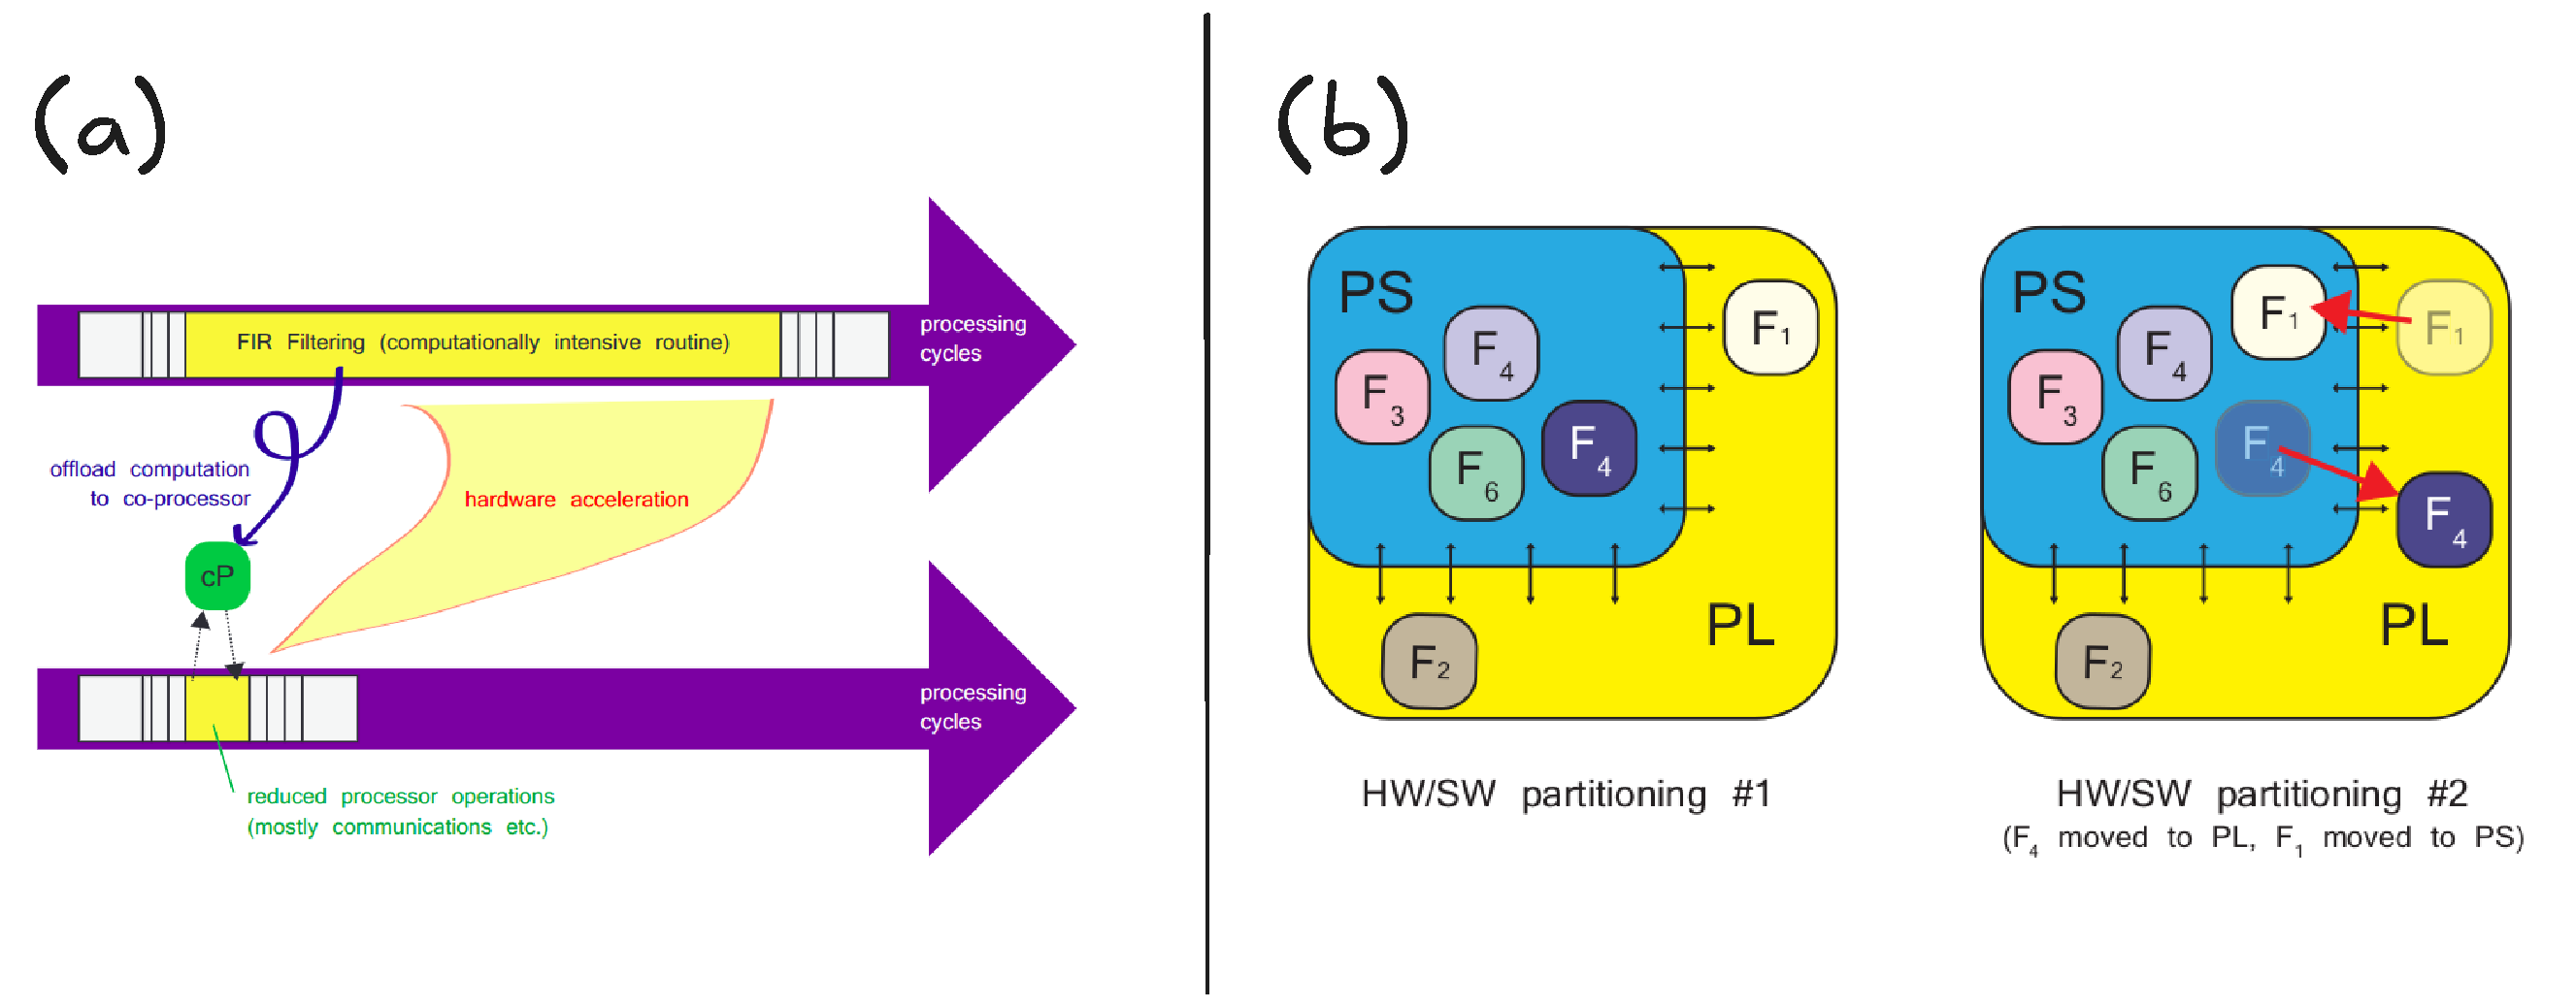
\includegraphics{cap2_offload_uc}
\caption[Aceleradores para reducir la carga de la CPU y particionado HW/SW]{%
Extraídas del ZynqBook~\cite[figs.~4.7 y 4.10]{Crockett2014}. (a)~Utilización
de aceleradores para reducir la carga de la CPU. Arriba, una rutina en la que
una gran parte del tiempo de ejecución está dedicada a una tarea específica, en
este caso un filtrado FIR. Abajo, el filtrado se delega a un coprocesador (cP) y
al procesador le quedan sólo las operaciones de comunicación. (b)~Dos
particionados de tareas HW/SW en un Zynq: en el segundo, F4 pasa a la PL y F1 al
PS.\label{f:hw-offload}}
\end{figure}

Sus usos son diversos, pero generalmente ocupan los siguientes nichos:
\begin{itemize}
  \item \textbf{Computación de baja latencia y determinista}: la respuesta tarda
    un número fijo de ciclos de reloj.
  \item Creación de \textbf{procesadores digitales personalizados de alto
    \emph{throughput}} (DSP).
  \begin{itemize}
    \item Escalabilidad: se pueden crear más canales instanciando más HW, en
      cambio con un µC agregar canales \textbf{quita} ciclos disponibles al
      presupuesto total.
  \end{itemize}
  \item \textbf{Ancho de banda}:
  \begin{itemize}
    \item El \emph{fabric} permite flujos de datos de alto \emph{throughput}. Ejemplo
      con el sistema actual: 125~MSPS $\times$ 14~bits $\approx$
      \textbf{1,75~Gbit/s} sostenidos por canal, 500~MB/s para los dos canales
      en palabras de 16 bits. Un µC no puede procesar ese caudal, y ni siquiera
      guardarlo para después: a ese ritmo, la SRAM del orden de 1~MB de un
      STM32H7 se llena en unos 2~ms.
  \end{itemize}
  \item Interfaz \textbf{directa con el mundo físico} (I/O):
  \begin{itemize}
    \item Necesitamos requisitos de \emph{timing} mucho más ajustados que los que puede
      cumplir una CPU. Incluye:
    \item Interfaz eléctrica del ADC.
  \end{itemize}
  \item \textbf{Descarga de la CPU} (\emph{offload}): la CPU queda libre para
    configurar el hardware, leer los resultados, guardarlos y presentarlos.
  \item Eficiencia energética (ops/W): se eliminan los \emph{fetch}/\emph{decode} de
    instrucciones y los accesos a caché.
  \item \textbf{Flexibilidad en el diseño} (propia de las FPGA): el hardware se
    reconfigura en campo con un \emph{bitstream} nuevo, sin cambiar la placa.
\end{itemize}

%%%%%%%%%%%%%%%%%%%%%%%%%%%%%%%%%%%%%%%%%%%%%%%%%%%%%%%%%%%%%%%%%%%%%%%%%%%%%%%%
\section{Plataformas de HW programable}
\label{S:hw-plataformas-programables}

Las FPGA nacieron en la década de los 80~\cite{Trimberger2015} como herramientas
que permiten la aceleración de hardware personalizada y a costo fijo bajo (entre
los cientos y miles de USD), mientras que los ASIC (\emph{Application Specific
Integrated Circuit}) cuestan entre 3-5 ordenes de magnitud más en su diseño y
producción.

\begin{figure}[H]
\centering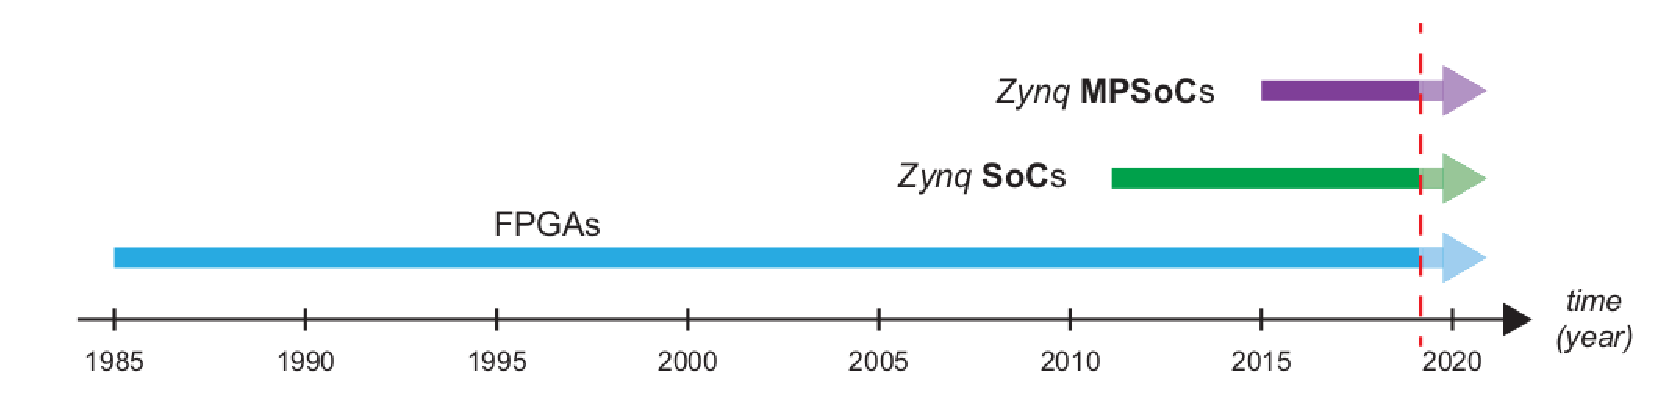
\includegraphics{cap2_historia_plataformas}
\caption[Línea de tiempo de las arquitecturas de HW programable]{%
Linea de tiempo con las principales arquitecturas HW programable.
\label{f:hw-historia}}
\end{figure}

En la Sec.~\ref{S:ap-hw-criterios} se encuentra una tabla exhaustiva de los
criterios de elección de la plataforma de HW~\cite{Crockett2014}; las categorías
principales son recursos computacionales, factores comerciales, facilidad diseño
y desarrollo, características físicas del dispositivo, flexibilidad. En la
Fig.~\ref{f:hw-familias-fpgas}(a) se muestran algunas familias de plataformas y
su aplicabilidad en los ejes capacidad del dispositivo (eje x) vs.\ la dificultad
en el diseño y desarrollo (eje y). En la Fig.~\ref{f:hw-familias-fpgas}(b) se
presenta la evolución de los recursos lógicos configurables, representados en
área.

\begin{figure}[H]
\centering
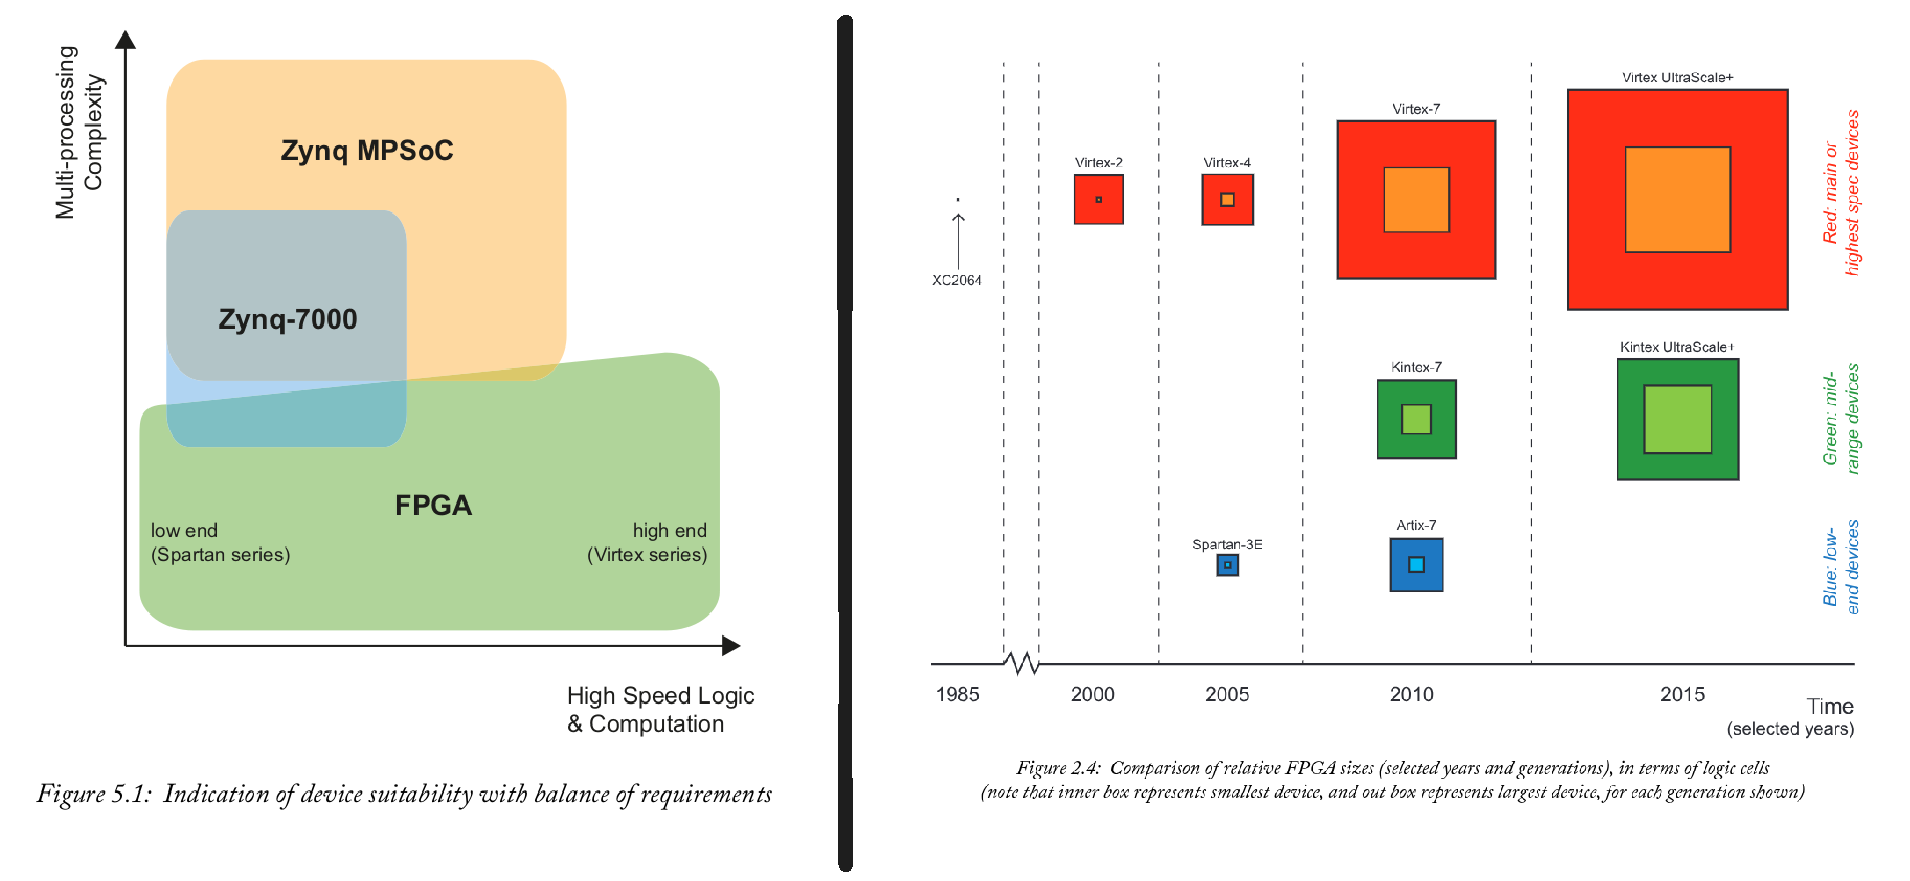
\includegraphics{cap2_familias_fpgas}
\caption[Elección de plataforma de HW programable y evolución de las FPGA]{%
(a)~Descripción cualitativa de la elección de plataforma de HW programable para
diferentes contextos de complejidad/\emph{performance}. (b)~Comparación del tamaño
relativo de los recursos lógicos de FPGA en años seleccionados.
\label{f:hw-familias-fpgas}}
\end{figure}

Es así que decidimos que la familia de placas de desarrollo Red Pitaya, que
contienen un SoC Zynq-7000, representa una buena plataforma de hardware para
este proyecto. A continuación se la describe en mayor detalle.

%%%%%%%%%%%%%%%%%%%%%%%%%%%%%%%%%%%%%%%%%%%%%%%%%%%%%%%%%%%%%%%%%%%%%%%%%%%%%%%%
\section{Plataforma empleada: Red Pitaya}
\label{S:hw-red-pitaya}

Una plataforma es un sistema especificado, con documentación y soporte, que
puede utilizarse como herramienta para resolver un problema. Nuestro proyecto
utiliza la Red Pitaya STEMlab 125-14; en la Fig.~\ref{f:hw-overview-pitaya} se
presenta una breve descripción de la placa. El chip cuadrado del centro, debajo
del disipador, es el SoC Zynq-7000: constituye el elemento central de
procesamiento de la plataforma, y a su alrededor están el resto de los
periféricos. Todos los modelos de Red Pitaya usan la misma familia de SoC,
Zynq-7000, pero no los mismos conversores ni el mismo front-end analógico
(Tabla~\ref{t:hw-modelos-pitaya}).

\begin{figure}[H]
\centering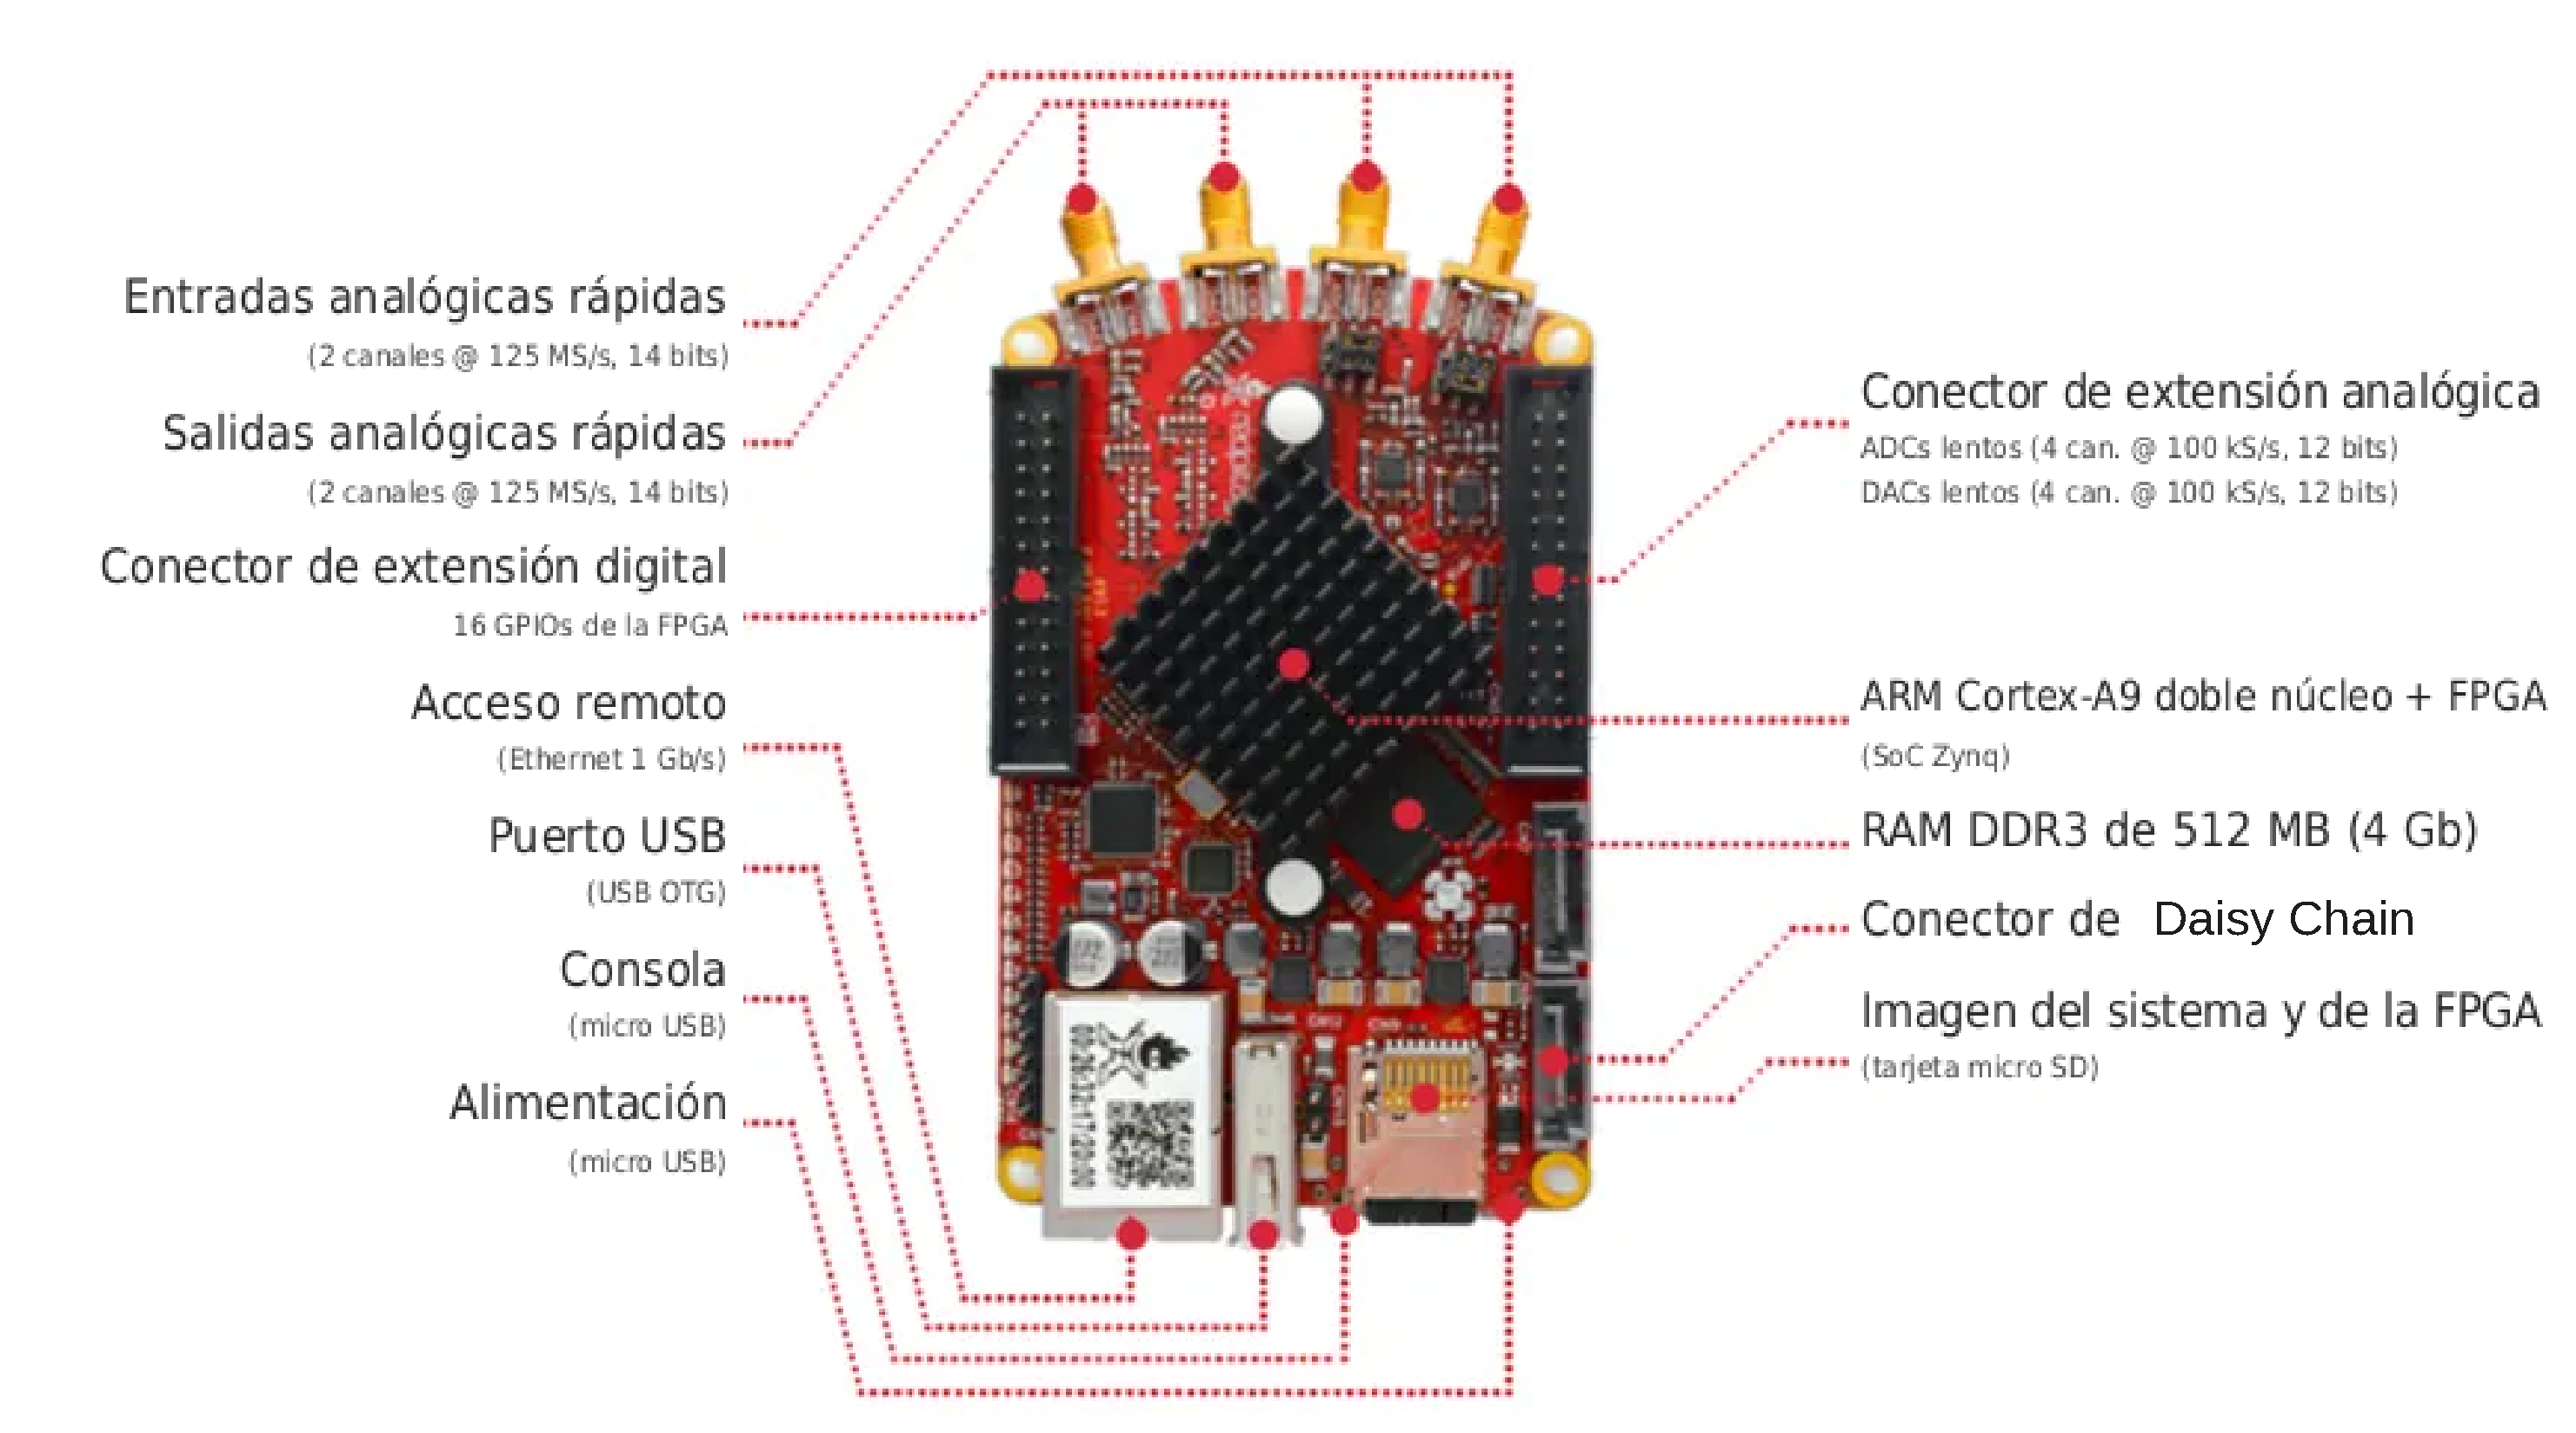
\includegraphics{cap2_overview_pitaya}
\caption[La placa STEMlab 125-14 y sus principales periféricos]{%
Foto de la placa de desarrollo STEMlab 125-14 y sus principales periféricos.
\label{f:hw-overview-pitaya}}
\end{figure}

Los principales cambios entre los modelos de Red Pitaya son los recursos de la
FPGA, las características del ADC, el tamaño de la RAM y la cantidad de
conectores digitales. En la Tabla~\ref{t:hw-modelos-pitaya} se presenta una
descripción general de las capacidades de las distintas placas.

\begin{table}[H]
\centering
\caption[Especificaciones de las placas Red Pitaya más comunes]{%
Especificaciones generales de las placas Red Pitaya más
comunes~\cite{RedPitayaDocs}.\label{t:hw-modelos-pitaya}}
\footnotesize
\setlength{\tabcolsep}{3pt}
\newcolumntype{Y}{>{\centering\arraybackslash}X}
\begin{tabularx}{\textwidth}{|>{\raggedright\arraybackslash}p{0.165\textwidth}|Y|Y|Y|Y|Y|Y|}
\hline
\encabezado \textbf{Característica} & \textbf{STEMlab 125-10}
  & \textbf{STEMlab 125-14} & \textbf{STEMlab 125-14 Z7020}
  & \textbf{STEMlab 125-14 4-Input} & \textbf{SDRlab 122-16}
  & \textbf{SIGNALlab 250-12} \\ \hline
SoC & Zynq 7010 & \textbf{Zynq 7010} & Zynq 7020 & Zynq 7020 & Zynq 7020
  & Zynq 7020 (grado -3) \\ \hline
RAM DDR3 & 256~MB & \textbf{512~MB} & 512~MB & 512~MB & 512~MB & 1~GB \\ \hline
ADC & 2~$\times$ 10 bit & \textbf{2~$\times$ 14 bit} & 2~$\times$ 14 bit
  & \textbf{4~$\times$ 14 bit} & 2~$\times$ 16 bit & 2~$\times$ 12 bit \\ \hline
Tasa ADC & 125~MS/s & \textbf{125~MS/s} & 125~MS/s & 125~MS/s & 122.88~MS/s
  & 250~MS/s \\ \hline
Ancho de banda & DC--50~MHz & \textbf{DC--60~MHz} & DC--60~MHz & DC--60~MHz
  & 300~kHz--550~MHz (AC) & DC--60~MHz \\ \hline
Rango de entrada & ±1~V / ±20~V & \textbf{±1~V / ±20~V} & ±1~V / ±20~V
  & ±1~V / ±20~V & 0.5~Vpp (50~$\Omega$) & ±1~V / ±20~V \\ \hline
DAC & 2~$\times$ 10 bit & \textbf{2~$\times$ 14 bit} & 2~$\times$ 14 bit & ---
  & 2~$\times$ 14 bit & 2~$\times$ 14 bit \\ \hline
Tasa DAC & 125~MS/s & \textbf{125~MS/s} & 125~MS/s & --- & 122.88~MS/s
  & 250~MS/s \\ \hline
GPIO (E1) & 16 & \textbf{16} & 22 & 22 & 22 & 19 \\ \hline
Ethernet & 1~Gbit & \textbf{1~Gbit} & 1~Gbit & 1~Gbit & 1~Gbit & 1~Gbit \\ \hline
USB & USB-A 2.0 & \textbf{USB-A 2.0} & USB-A 2.0 & USB-A 2.0 & USB-A 2.0
  & 2~$\times$ USB-A 2.0 \\ \hline
Alimentación & 5~V, 1.5~A & \textbf{5~V, 2~A} & 5~V, 2~A & 5~V, 2~A & 5~V, 2~A
  & 24~V, 0.5~A \\ \hline
Temperatura & 0--55~°C & \textbf{0--55~°C} & 0--55~°C & 0--55~°C & 0--55~°C
  & 0--55~°C \\ \hline
\end{tabularx}
\end{table}

En la Sec.~\ref{S:hw-perifericos} se describen en detalle los periféricos; vamos
a arrancar describiendo al protagonista del sistema en la Sec.~\ref{S:hw-soc}.

%%%%%%%%%%%%%%%%%%%%%%%%%%%%%%%%%%%%%%%%%%%%%%%%%%%%%%%%%%%%%%%%%%%%%%%%%%%%%%%%
\section{Arquitectura SoC: FPGA + µC}
\label{S:hw-soc}

Cuando se requería un hilo de trabajo secuencial y programable en una FPGA, se
sintetizaba un procesador sobre su \emph{fabric}. Estos procesadores se denominan
\emph{softcore} porque se construyen con los bloques maleables del \emph{fabric}; su
contrapunto son los \emph{hardcore}, implementados como ASIC, con una
funcionalidad completamente fijada por el fabricante.

Antes de que el procesador viniera integrado en el mismo chip, los softcores
eran la forma habitual de agregarle uno a una FPGA, y se siguen usando
(MicroBlaze~\cite{UG984}, Nios, núcleos RISC-V) para las siguientes actividades:
\begin{itemize}
  \item Lógica lenta pero de muchos pasos y ramificaciones.

    El ejemplo típico es cuando tenemos una tarea que requiere un algoritmo
    recursivo, es común resolver esto mediante la creación de un \emph{stack} dedicado
    por módulo, esto tiene la contra de que tenemos una región de memoria de uso
    extremadamente bajo y probablemente reducida para el trabajo de la tarea. Un
    CPU podría hacer uso de una memoria compartida, como es una RAM de forma de
    no tener estas limitaciones.
  \item Iterar sin re-sintetizar.
  \item Configurabilidad e instrucciones \emph{custom}.
  \item Múltiples \emph{cores} dedicados.
\end{itemize}

Esto nos dice algo muy importante de la estructura del HW, siempre que queremos
un elemento de control lo podemos sintetizar de manera independiente. Y esto
ocurre muy a menudo, por ejemplo cuando necesitamos mover datos en grandes
cantidades paquetes y de manera no continua se define un subsistema de memoria
llamado DMA, \emph{Direct Memory Access}, el cual toma el rol del CPU pero para
transferencias de datos. Este sería un acelerador pero de transferencia de
datos.

El problema principal de los softcores es el rendimiento. En la
Fig.~\ref{f:hw-softcore}(b) se compara el rendimiento del \textbf{mejor caso} de
tres familias de procesadores: en rosa el ARM Cortex-A9, el presente en este
trabajo; en gris el PowerPC de la Virtex-5, un procesador duro embebido en el
\emph{fabric}; y en azul oscuro tres softcores. Entre 2002 y 2010 hubo varias FPGA con
procesadores duros de este tipo (PowerPC 405 y 440 en las Virtex-II
Pro~\cite{DS083}, Virtex-4 FX y Virtex-5 FXT~\cite{UG200}); el Zynq-7000 (2011)
fue un paso más, con un sistema de procesamiento completo en el mismo chip.

\begin{figure}[H]
\centering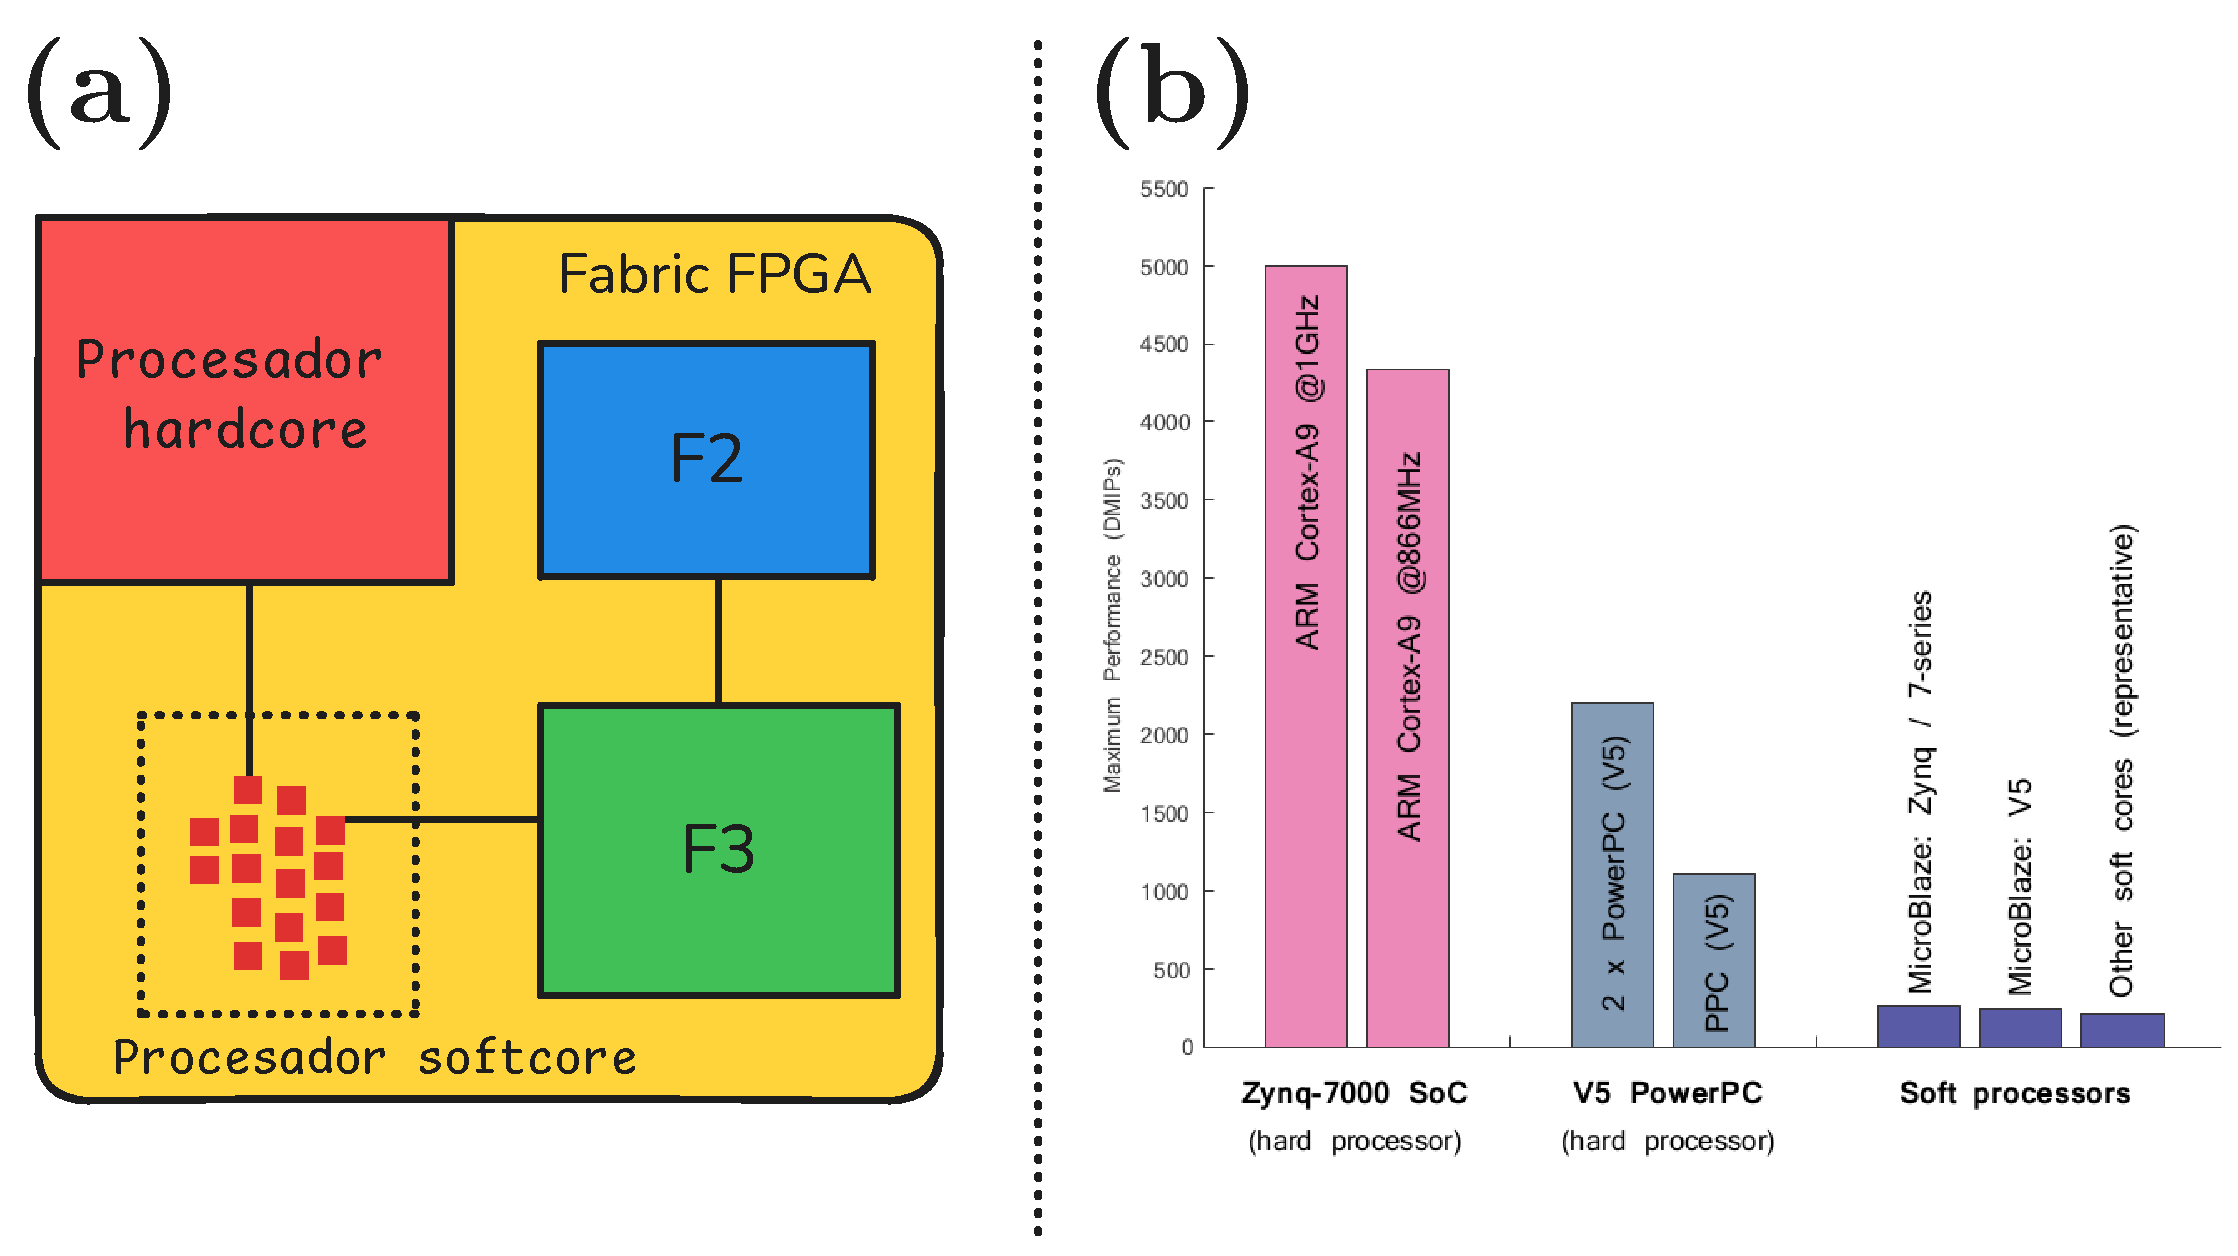
\includegraphics{cap2_softcore_hardcore}
\caption[Procesadores softcore y hardcore]{%
Comparación de procesadores softcore y hardcore. (a)~Comparación dentro de un
SoC: el procesador hardcore tiene su propia región del chip, dedicada e
inmodificable, y el procesador softcore ocupa lugar de la \emph{fabric} al lado de
otros módulos de HW, F2 y F3. (b)~Rendimiento máximo, en DMIPS
(\emph{Dhrystone millions of instructions per second}, un \emph{test} estandarizado de
\emph{performance}~\cite{Weicker1984}), de procesadores hardcore ---el Cortex-A9 del PS
del Zynq-7000, en rosa, y el PowerPC embebido en el \emph{fabric} de la Virtex-5, en
gris--- contra procesadores softcore instanciados en la PL, en azul oscuro.
Valores indicativos, del mejor caso. Extraída del
ZynqBook~\citefig{Crockett2014}{4.3}.\label{f:hw-softcore}}
\end{figure}

El punto a notar es que el Cortex-A9 doble rinde, en el mejor caso, entre 16 y
24 veces lo que un softcore; los dos núcleos de la placa, a 667~MHz, rinden unas
12 veces lo que un MicroBlaze. Un softcore con MMU, como el MicroBlaze, también
puede correr Linux~\cite{UG984}: lo que cambia con el hardcore es el
rendimiento, que alcanza para que nuestro sistema deje de trabajar como un
embebido y comience a funcionar como una computadora dedicada, con un sistema
operativo completo.

\subsection{Arquitectura del Zynq-7000}
\label{S:hw-zynq}

Aun siendo los dos sistemas de procesamiento, sus características son
extremadamente diferentes. Con el tiempo se vio el beneficio de acortar el
enlace entre ambos, y terminaron en el mismo encapsulado. Al estar en un mismo
chip cambió la forma típica de uso, y se les dieron nuevos nombres: la FPGA pasó
a llamarse \emph{programmable logic} (PL) y el procesador, \emph{processing
system} (PS)~\cite{UG585}.

\begin{figure}[H]
\centering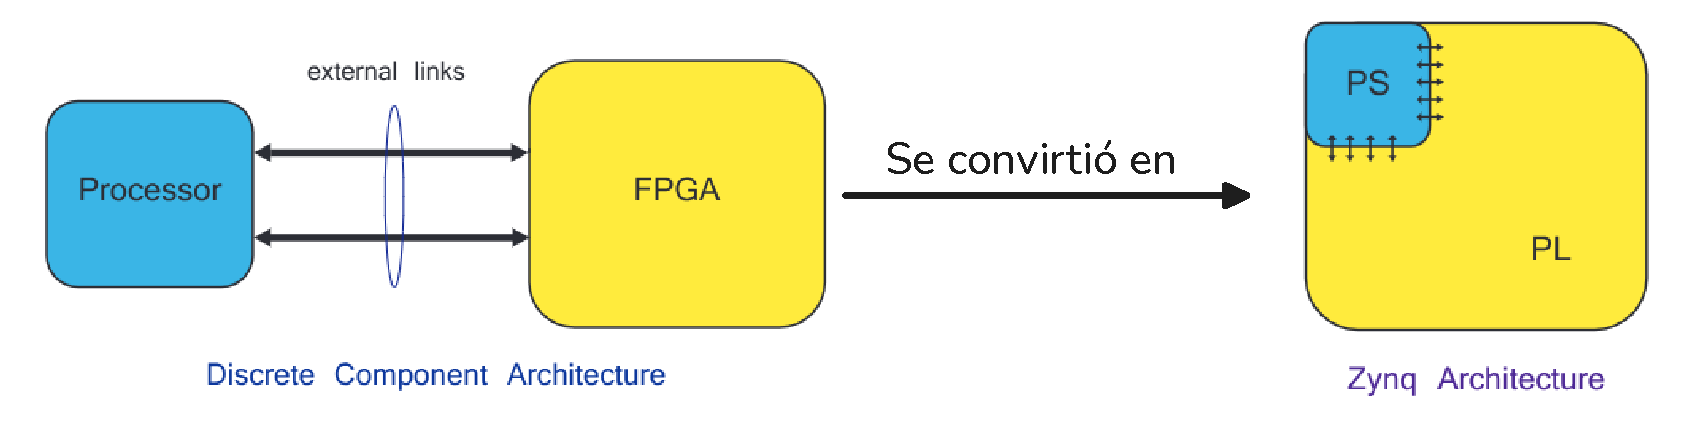
\includegraphics{cap2_arquitectura_zynq}
\caption[Combinación de procesador y FPGA]{%
Combinación de procesador + FPGA con enlaces externos a un chip.
\label{f:hw-arquitectura-zynq}}
\end{figure}

Los diferentes periféricos y módulos se conectan a una \textbf{red de
direccionamiento} interna del sistema llamada \emph{interconnect}, cuyo
funcionamiento es análogo al de los \emph{switches} de una red de computadoras: su
objeto es almacenar temporalmente (\emph{buffer}) y redireccionar las
transacciones para que la comunicación en el sistema sea eficiente. El
direccionamiento se hace mediante \textbf{direcciones}: cada módulo está
\textbf{mapeado en memoria}, es decir, tiene un conjunto de direcciones fijas.
Estas direcciones corresponden a registros clave expuestos al exterior, que
generalmente se llaman de \textbf{control} o de \textbf{estado}.

Todo lo que trabaje con el protocolo del \emph{interconnect} se puede conectar, y eso
es parte de su capacidad de extensión: generalmente se lo define con capacidad
para N conexiones esclavas y M maestras. En la
Fig.~\ref{f:hw-interconexiones-soc} se presentan distintos tipos de periféricos,
procesadores y memorias que comparten el mismo tipo de \emph{interconnect}.

\begin{figure}[H]
\centering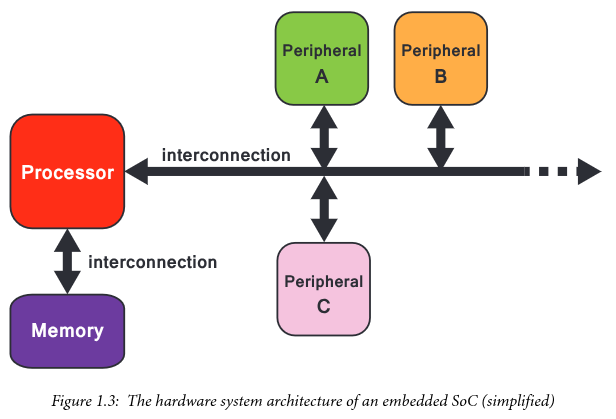
\includegraphics{cap2_interconexiones_soc}
\caption[Representación de un SoC]{%
Representación de un SoC. Extraído del ZynqBook~\cite{Crockett2014}.
\label{f:hw-interconexiones-soc}}
\end{figure}

El procesador principal en este proyecto es la PL así que vamos a comenzar
describiendo sus características, recursos e interfaces externas.

\subsection{Arquitectura de la lógica programable (PL)}
\label{S:hw-pl}

Parte de la potencia de la FPGA es su flexibilidad, que se obtiene mediante la
\textbf{configuración de los recursos lógicos programables}. En la
Tabla~\ref{t:hw-recursos-pl} se presentan los recursos de los dos Zynq de la
familia Red Pitaya.

\begin{table}[H]
\centering
\caption[Recursos lógicos de los Zynq de las placas Red Pitaya]{%
Recursos lógicos de los dos Zynq presentes en las placas Red
Pitaya~\cite{DS190}.\label{t:hw-recursos-pl}}
\small
\begin{tabular}{|l|r|r|c|}
\hline
\encabezado \textbf{Recurso de la PL} & \textbf{XC7Z010} & \textbf{XC7Z020}
  & \textbf{$\times$} \\ \hline
Celdas lógicas (unidad comercial, $\approx$ 1,6 LUT6) & 28\,k & 85\,k & 3.0 \\ \hline
CLB & 2\,200 & 6\,650 & 3.0 \\ \hline
\emph{Slices} (2 por CLB) & 4\,400 & 13\,300 & 3.0 \\ \hline
LUT6 & 17\,600 & 53\,200 & 3.0 \\ \hline
Flip-flops & 35\,200 & 106\,400 & 3.0 \\ \hline
Block RAM (RAMB36) & 60 (2.1~Mb) & 140 (4.9~Mb) & 2.3 \\ \hline
DSP48E1 & 80 & 220 & 2.75 \\ \hline
PLL / MMCM & 2 / 2 & 4 / 4 & 2 \\ \hline
\end{tabular}
\end{table}

El bloque básico del tejido lógico es el \textbf{\emph{Configurable Logic Block}
(CLB)}~\cite{UG474}. Cada CLB contiene \textbf{dos \emph{slices}} y se conecta
al resto del dispositivo a través de una \textbf{matriz de conmutación}
(\emph{switch matrix}), que es su único acceso a la red de interconexión
general; en la Sec.~\ref{S:ap-hw-clb} se describen más detalles. Estos
bloques están distribuidos por el cuerpo de la FPGA. En la
Fig.~\ref{f:hw-bloques-fpga}(b) se ve el \emph{fabric} en forma de L: la esquina
faltante del rectángulo del die la ocupa físicamente el PS. El tejido está
organizado en filas y columnas de dimensiones cuantizadas; dentro de esa grilla
se colocan bloques del mismo tipo a lo largo de columnas enteras (una columna de
CLB, una columna de Block RAM, una columna de DSP), y las columnas están
separadas por canales de interconexión a los que se accede por las matrices de
conmutación.

\begin{figure}[H]
\centering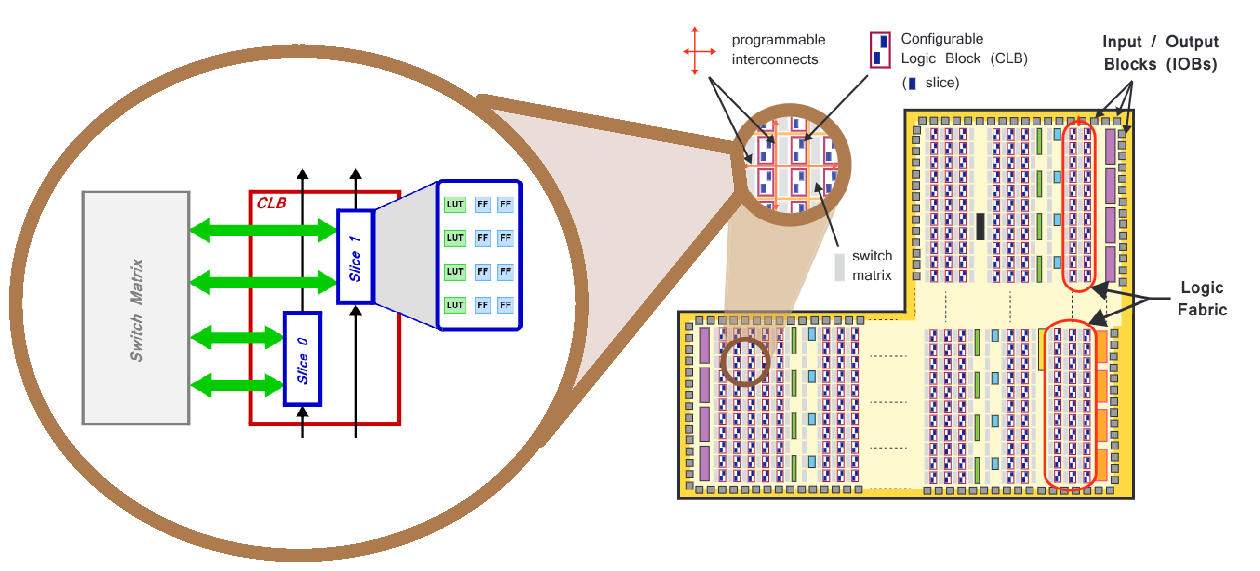
\includegraphics{cap2_bloques_basicos_fpga}
\caption[Bloques básicos de la FPGA]{%
Bloques básicos de la FPGA. (a)~Composición elemental de una CLB. (b)~\emph{Fabric}
del Zynq7010 y sus elementos constitutivos básicos. Estos incluyen las CLBs y
interconexiones programables.\label{f:hw-bloques-fpga}}
\end{figure}

Además del \emph{fabric} genérico, la arquitectura incorpora bloques duros
(\emph{hard macros}), optimizados para funciones que serían caras de construir
con LUT, en la Tabla~\ref{t:hw-hardmacros} se presentan las que se utilizaron
para este proyecto.

\begin{table}[H]
\centering
\caption[Hardmacros especializadas dentro de la PL del Zynq]{%
Hardmacros especializadas dentro de la PL del
Zynq~\cite{UG473,UG479,UG472,UG471,UG480}.\label{t:hw-hardmacros}}
\small
\begin{tabularx}{\textwidth}{|>{\raggedright\arraybackslash}p{0.17\textwidth}|>{\raggedright\arraybackslash}X|>{\raggedright\arraybackslash}p{0.2\textwidth}|}
\hline
\encabezado \textbf{Recurso} & \textbf{Qué es} & \textbf{Presentes en XC7Z010} \\ \hline
\textbf{Block RAM} & Memorias de 36~Kb, divisibles en dos de 18~Kb, de
  \textbf{doble puerto verdadero}, con ancho de palabra configurable y modo FIFO
  integrado & 60 bloques (2.1~Mb) \\ \hline
\textbf{DSP48E1} & Pre-sumador + multiplicador con signo de \textbf{25~$\times$
  18 bits} + acumulador de 48 bits, encadenables entre sí sin pasar por el
  tejido & 80 \\ \hline
\textbf{\emph{Clock tiles} (CMT)} & gestión de reloj: MMCM y PLL, que sintetizan,
  multiplican y desfasan relojes & 2 MMCM + 2 PLL \\ \hline
\textbf{\emph{Buffers} de reloj} & BUFG (red global), BUFH (regional), BUFR/BUFIO (de
  entrada/salida) & 32 BUFG, 48 BUFH, 8 BUFR, 8 BUFIO \\ \hline
\textbf{IOB} & bloques de entrada/salida, con registros propios
  (ILOGIC/OLOGIC), serializadores (ISERDES/OSERDES), dobladores de tasa
  (IDDR/ODDR) y líneas de retardo calibradas (IDELAY) & 100 pines utilizables
  \\ \hline
\textbf{XADC} & ADC de 12 bits y 1~MS/s integrado, con sensores internos de
  temperatura y tensión & 1 \\ \hline
\end{tabularx}
\end{table}

En nuestra aplicación usamos tanto los recursos de entrada a la PL, con las
conexiones del ADC, como los de salida de la PL, con la conexión al PS. Se
describen en la Sec.~\ref{S:hw-interconexiones}.

\subsection{Interconexiones presentes}
\label{S:hw-interconexiones}

En la Fig.~\ref{f:hw-interfaces-zynq}(a) se presenta buena parte de las
interconexiones internas y externas del Zynq-7010. Las más importantes para este
proyecto son las interfaces AXI (\emph{Advanced eXtensible Interface}), las
principales entre el PS y la PL. AXI es una familia de estándares
AMBA~\cite{AMBAAXI} de \textbf{buses intrachip} de \textbf{alta \emph{performance}} y
de tipo \textbf{punto a punto}. En la Fig.~\ref{f:hw-interfaces-zynq}(b) se
presentan las nueve interfaces AXI del sistema, que se dividen en tres grupos:
\emph{general purpose} (GP), \emph{high performance} (HP) y \emph{accelerator
coherency port} (ACP).

\begin{figure}[H]
\centering
\begin{minipage}[b]{0.56\textwidth}\centering
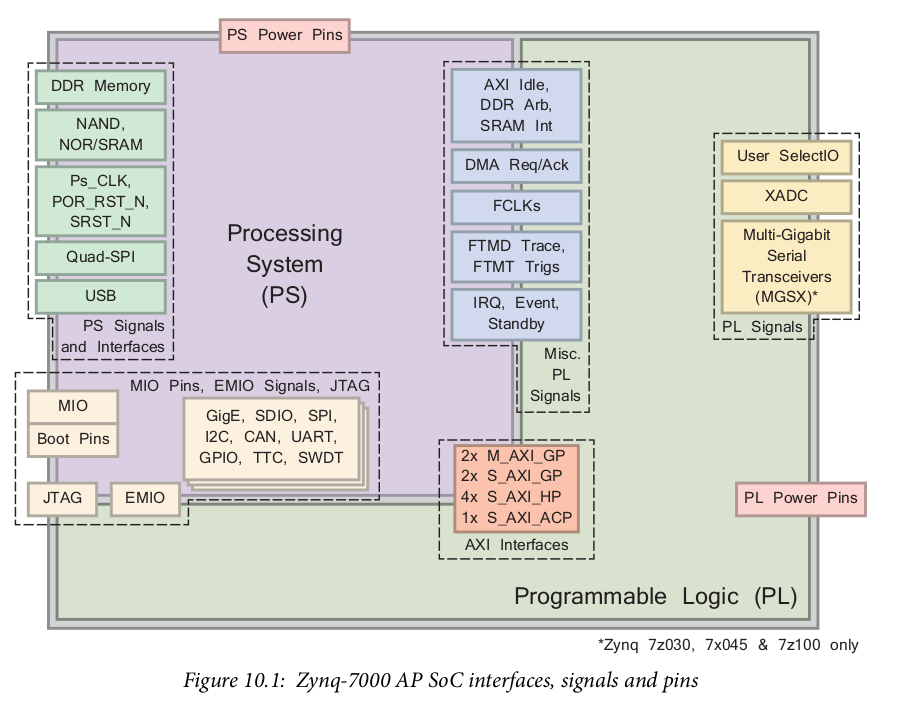
\includegraphics[width=\linewidth]{cap2_interfaces_zynq}\\(a)
\end{minipage}\hfill
\begin{minipage}[b]{0.42\textwidth}\centering
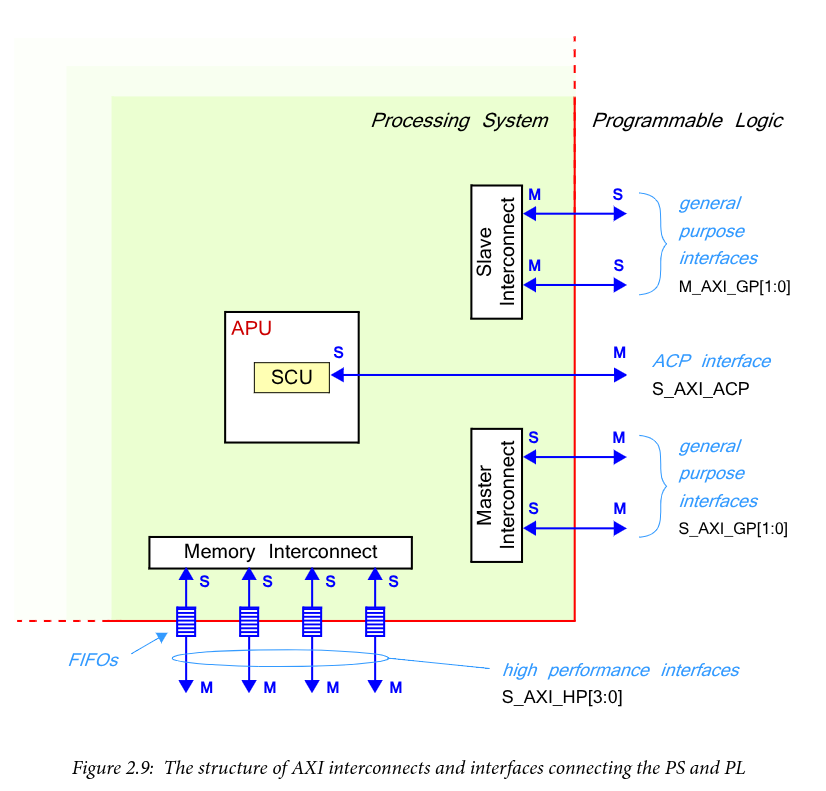
\includegraphics[width=\linewidth]{cap2_interfaces_axi}\\(b)
\end{minipage}
\caption[Interfaces del SoC e interfaces AXI entre el PS y la PL]{%
(a) Interfaces internas y externas del SoC. Extraído del
ZynqBook~\citefig{Crockett2014}{10.1}. (b) Interfaces AXI entre el PS y la PL
del SoC, descritas en detalle en la Tabla~\ref{t:hw-axi}.\label{f:hw-interfaces-zynq}}
\end{figure}

Las características principales de cada una se describen en la
Tabla~\ref{t:hw-axi}. Las mayores diferencias son el \textbf{\emph{throughput} máximo
obtenible}, la \textbf{latencia de acceso} y la cantidad de conexiones
disponibles.

\begin{table}[H]
\centering
\caption[Propiedades de las interconexiones AXI entre el PS y la PL]{%
Propiedades de las interconexiones AXI entre el PS y la PL~\cite{UG585}. El
esclavo de Red Pitaya está en su repositorio~\cite{RedPitayaFPGA}.
\label{t:hw-axi}}
\footnotesize
\setlength{\tabcolsep}{3pt}
\newcolumntype{Y}{>{\raggedright\arraybackslash}X}
\begin{tabularx}{\textwidth}{|>{\raggedright\arraybackslash}p{0.13\textwidth}|Y|Y|Y|Y|}
\hline
\encabezado & \codigo{M\_AXI\_GP} & \codigo{S\_AXI\_GP} & \codigo{S\_AXI\_HP}
  & \codigo{S\_AXI\_ACP} \\ \hline
\textbf{Ancho de bus} & 32 bit & 32 bit & \textbf{64 bit} (configurable 32/64)
  & 64 bit \\ \hline
\textbf{Techo teórico} & 32~b $\times$ 150~MHz = \textbf{600~MB/s} & 600~MB/s
  & 64~b $\times$ 150~MHz = \textbf{1200~MB/s} por puerto & 1200~MB/s \\ \hline
\textbf{Ráfagas} & las admite AXI, \textbf{pero el esclavo de Red Pitaya no}
  & sí & \textbf{sí}, hasta 16 \emph{beats}, con FIFO de lectura y de escritura
  & sí \\ \hline
\textbf{Caso de uso típico} & \textbf{registros de control y estado}; lecturas
  chicas y esporádicas & que la PL acceda a periféricos del PS u OCM
  & \textbf{volcado masivo a DDR}: captura de ADC, video, DMA
  & acelerador que comparte estructuras con el CPU sin invalidar caché \\ \hline
Cantidad disponibles & 2 & 2 & 4 & 1 \\ \hline
\end{tabularx}
\end{table}

Para conectar múltiples puntos entre sí con una topología modificable se suelen
utilizar IP dedicadas, los \emph{interconnects} de Xilinx~\cite{PG059}. La
versión más empleada es el \textbf{\emph{crossbar}}, que puede observarse en la
Fig.~\ref{f:hw-topologia}(a): tiene una forma ``matricial'', con filas, columnas
y un interruptor en cada intersección que conecta ese vértice; canalizando bien
las transacciones podemos conectar varios pares de elementos de forma
simultánea. En la Fig.~\ref{f:hw-topologia}(b) se presenta la topología
estrella, que necesita muchas menos trazas a nivel de silicio pero sólo puede
comunicar un par de puntos a la vez. Vamos a ver en la
Sec.~\ref{S:intro-hw-bus-custom} que Red Pitaya utiliza esta topología para su bus \emph{custom}.

\begin{figure}[H]
\centering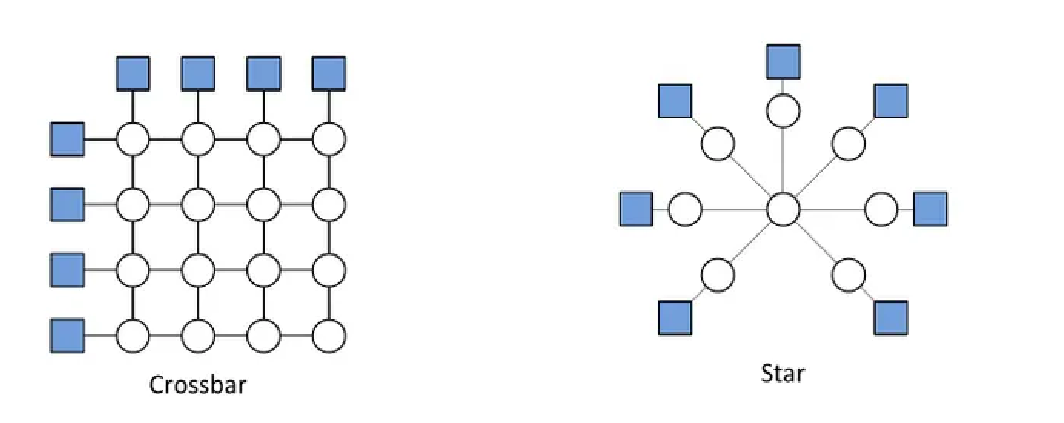
\includegraphics{cap2_topologia_interconnect}
\caption[Tipos de \emph{interconnects} más utilizados dentro del HW]{%
Tipos de \emph{interconnects} más utilizados dentro del HW. (a)~Interconexionado
\emph{crossbar}. (b)~Interconexionado estrella.\label{f:hw-topologia}}
\end{figure}

\subsection{Procesador Cortex-A9}
\label{S:hw-cortex-a9}

El Cortex-A9, anunciado en 2007, fue el núcleo de alta gama de la arquitectura
\textbf{ARMv7-A} (presentada en 2005 con el Cortex-A8) hasta la llegada del
Cortex-A15. Está diseñado para correr sistemas operativos
completos~\cite{DDI0388}. El Zynq-7010 de la placa trae \textbf{dos núcleos a
667~MHz} (grado de velocidad $-1$)~\cite{DS190}. La jerarquía de memoria del
procesador se presenta en la Fig.~\ref{f:hw-memoria-a9}.

\begin{figure}[H]
\centering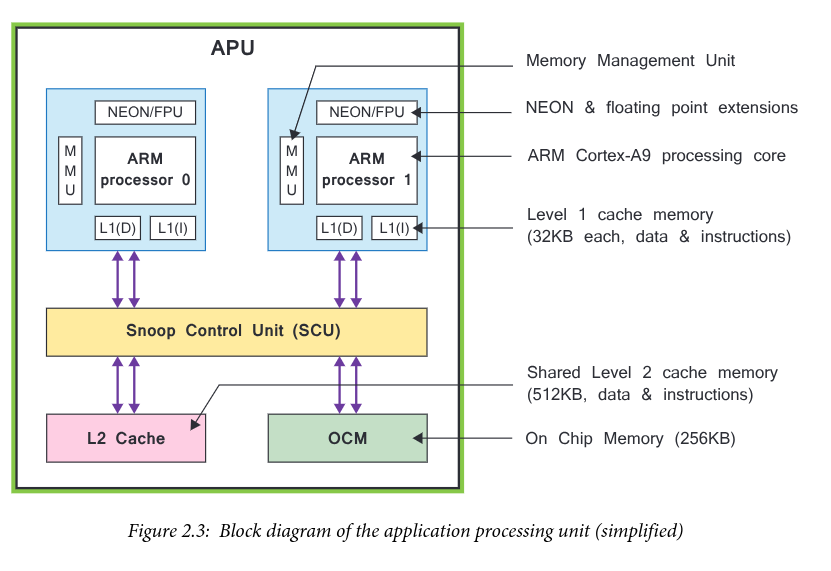
\includegraphics{cap2_jerarquia_memoria_a9}
\caption[Jerarquía de la memoria del APU]{%
Jerarquía de la memoria del APU.\label{f:hw-memoria-a9}}
\end{figure}

El tamaño de cada bloque condiciona en gran medida el rendimiento real. En orden
creciente de tamaño y de tiempo de acceso están la caché de nivel 1 (L1), la
caché de nivel 2 (L2), la memoria en chip (OCM) y la DDR3 externa; sus
características se presentan en la Tabla~\ref{t:hw-memorias}.

\begin{table}[H]
\centering
\caption[Niveles de memoria del PS del Zynq-7010]{%
Niveles de memoria del PS del Zynq-7010 en la STEMlab
125-14~\cite{UG585}.\label{t:hw-memorias}}
\small
\begin{tabularx}{\textwidth}{|l|l|>{\raggedright\arraybackslash}X|>{\raggedright\arraybackslash}X|}
\hline
\encabezado \textbf{Nivel} & \textbf{Tamaño} & \textbf{Organización}
  & \textbf{Alcance} \\ \hline
\textbf{L1 instrucciones} & 32~KB por núcleo & 4 vías & privado de cada núcleo \\ \hline
\textbf{L1 datos} & 32~KB por núcleo & 4 vías & privado de cada núcleo \\ \hline
\textbf{L2 unificada} & 512~KB & 8 vías (controlador PL310)
  & compartida por los dos núcleos \\ \hline
\textbf{OCM} & 256~KB & SRAM en el die, sin caché
  & los dos núcleos \textbf{y la PL} \\ \hline
\textbf{DDR3 externa} & 512~MB en esta placa & 16 bits a 533~MHz
  & $\sim$2.1~GB/s de pico teórico \\ \hline
\end{tabularx}
\end{table}

Cada núcleo tiene una \emph{memory management unit} (MMU)~\cite{DDI0406C}, que
traduce, página por página, las direcciones \textbf{virtuales} que usa el
software a las direcciones \textbf{físicas} que salen al bus. Sus tareas son:
\begin{enumerate}
  \item \textbf{Aislamiento}: cada \textbf{proceso} tiene su propio mapa de
    memoria virtual y no puede nombrar la memoria de otro proceso. Los dos
    núcleos, en cambio, comparten la memoria física y el mismo \emph{kernel}; por eso
    hace falta la SCU que se describe más abajo.
  \item \textbf{Eficiencia en el manejo de memoria}: el sistema operativo asigna
    la memoria en páginas, asocia cada región virtual contigua a páginas físicas
    que pueden estar dispersas y puede reubicarlas sin que el programa se
    entere.
  \item \textbf{Manejo de atributos por página}: cada página cuenta con banderas
    que determinan permisos (acceso: lectura/escritura/ejecución, y modo:
    usuario/privilegiado) y el \textbf{tipo de memoria}, esta categoría se
    explica en la Sec.~\ref{S:hw-modelo-memoria}.
\end{enumerate}

En este proyecto la MMU es el mecanismo por el cual el software llega a la PL:
abrir \ruta{/dev/mem} y hacer \codigo{mmap} de \codigo{0x4000\_0000} le pide a
la MMU una entrada de tabla que apunte a los registros de la PL, marcada como no
cacheable.

Mientras que la \emph{Snoop Control Unit} (SCU)~\cite{DDI0407}
\textbf{mantiene coherentes} las cachés L1 de datos de los dos núcleos, es
decir, garantiza que cada dirección de memoria tenga un único valor vigente.
Para lograrlo guarda una copia duplicada de los \emph{tags} de las dos L1: de forma que
sabe en todo momento qué líneas tiene cada núcleo, y así puede husmear
(\emph{snooping}) \textbf{sólo al que corresponde} en cada acceso conflictivo.
Qué accesos identifica el sistema como conflictivos depende del esquema de
coherencia por línea de caché, el más conocido es \textbf{MESI}
(\emph{Modified / Exclusive / Shared / Invalid}), para más info se refiere al
libro de Nagarajan et al.~\cite{Nagarajan2020}.

Su arquitectura de conjunto de instrucciones (ISA) es la combinación de
diferentes subconjuntos con objetivos específicos, presentados en la
Tabla~\ref{t:hw-isa}~\cite{DDI0406C}.

\begin{table}[H]
\centering
\caption[Conjuntos de instrucciones del Cortex-A9 y su uso en el proyecto]{%
Diferentes conjuntos de ISA estándares, la funcionalidad y criterio de diseño
empleados y la utilización de los mismos en el proyecto actual.
\label{t:hw-isa}}
\small
\begin{tabularx}{\textwidth}{|>{\raggedright\arraybackslash}p{0.17\textwidth}|>{\raggedright\arraybackslash}X|>{\raggedright\arraybackslash}X|}
\hline
\encabezado \textbf{Conjunto} & \textbf{Qué es}
  & \textbf{Utilización en el proyecto} \\ \hline
\textbf{ARM (A32)} & Instrucciones de 32 bits de ancho fijo, ejecución
  condicional en casi todas & Sólo si se compila con \codigo{-marm} \\ \hline
\textbf{Thumb-2} & mezcla de 16 y 32 bits: $\sim$30~\% menos código con
  rendimiento equivalente & El que genera gcc por defecto en armhf
  (Ubuntu/Debian)~\cite{DebianArmHF}: el código de Linux y el de este proyecto
  \\ \hline
\textbf{VFPv3} & unidad de punto flotante IEEE-754, simple y \textbf{doble}
  precisión, 32 registros de 64 bits & \codigo{double} de C, \codigo{float64}
  de NumPy \\ \hline
\textbf{NEON (Advanced SIMD)} & SIMD de 128 bits: 16 registros Q de 128 bits,
  alias de 32 registros D de 64. Enteros de 8/16/32/64 bits y flotante de
  \textbf{simple precisión} & Lo que vectoriza NumPy en float32 y en enteros;
  no en float64, su tipo por defecto, porque NEON de ARMv7 no tiene doble
  precisión \\ \hline
\textbf{TrustZone} & extensiones de seguridad, mundo seguro/no seguro & --- \\ \hline
\textbf{Jazelle / ThumbEE} & ejecución de bytecode, heredados y obsoletos
  & --- \\ \hline
\end{tabularx}
\end{table}

\subsection{Modelo de memoria}
\label{S:hw-modelo-memoria}

ARMv7 distingue tres \textbf{tipos de memoria}, y el tipo lo fija la tabla de
páginas de la \emph{Memory Management Unit} (MMU):

\begin{table}[H]
\centering
\caption[Modelo de memoria de ARMv7]{%
Modelo de memoria de ARMv7~\cite{DDI0406C}.\label{t:hw-modelo-memoria}}
\small
\begin{tabularx}{\textwidth}{|l|X|}
\hline
\encabezado \textbf{Tipo} & \textbf{Qué permite el procesador} \\ \hline
\textbf{Normal} & reordenar, fusionar, especular, cachear, leer de más
  (\emph{prefetch}) \\ \hline
\textbf{\emph{Device}} & sin reordenamiento entre accesos, sin fusión, sin
  especulación, sin acceso adelantado \\ \hline
\textbf{\emph{Strongly-ordered}} & como \emph{Device}, y además el acceso no se completa
  hasta llegar al destino \\ \hline
\end{tabularx}
\end{table}

Esto es importante porque los registros de la PL se acceden con un tipo de
memoria sin caché: \textbf{\emph{Device}} si los mapea un \emph{driver} del \emph{kernel}
(\codigo{ioremap}), y \textbf{\emph{Strongly-ordered}} si, como en este proyecto, se
mapean desde el espacio de usuario con \codigo{mmap} sobre
\ruta{/dev/mem}~\cite{LinuxMMU}. Ninguno de los dos tipos impide que el
compilador emita instrucciones de acceso múltiple
(\codigo{LDM}/\codigo{STM}) o de NEON: la arquitectura las permite, y en el bus
AXI se convierten en ráfagas o accesos anchos que el esclavo de Red Pitaya no
acepta. Si no lo tenemos en cuenta podemos tener problemas graves, como los
presentados en la Sec.~\ref{S:intro-hw-modos-falla}, que llegan hasta un reinicio completo
del sistema.

%%%%%%%%%%%%%%%%%%%%%%%%%%%%%%%%%%%%%%%%%%%%%%%%%%%%%%%%%%%%%%%%%%%%%%%%%%%%%%%%
\section{Periféricos externos a la Pitaya}
\label{S:hw-perifericos}

Para describirlos nos referimos al diagrama en bloques de la placa, presentado
en la Fig.~\ref{f:hw-diagrama-bloques}.

\begin{figure}[H]
\centering
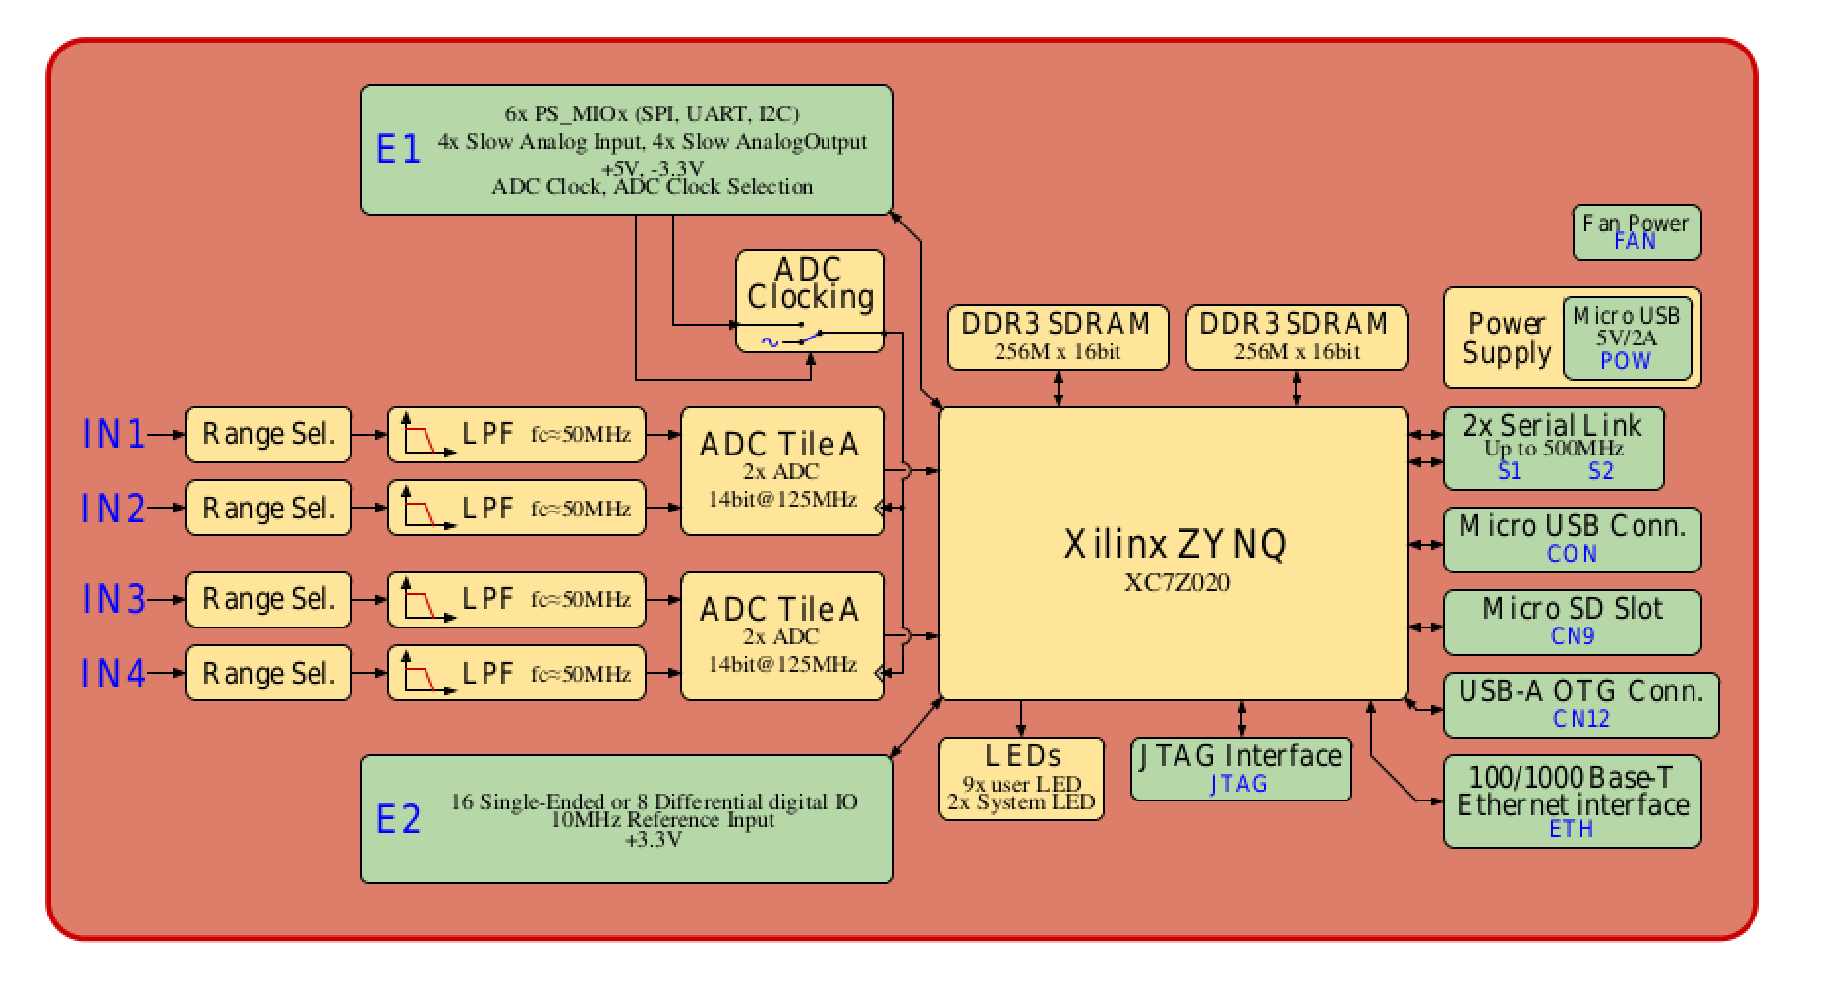
\includegraphics{cap2_diagrama_bloques_pitaya}
\caption[Diagrama de bloques de la plataforma]{%
Diagrama de bloques de la plataforma.\label{f:hw-diagrama-bloques}}
\end{figure}

\subsection{Entrada analógica presente: ADC}
\label{S:hw-adc}

La señal digitalizada es la base del procesamiento en todo el dispositivo. La
STEMlab 125-14 (y sus variantes Z7020 y 4-Input) usa el conversor
analógico-digital (ADC) LTC2145-14 de Analog Devices~\cite{LTC2145}; los otros
modelos cambian de conversor (Tabla~\ref{t:hw-modelos-pitaya}). Sus
características principales se presentan en la Tabla~\ref{t:hw-ltc2145}.

\begin{table}[H]
\centering
\caption[Características del ADC LTC2145-14 y del front-end de entrada]{%
Características principales del ADC LTC2145-14 y del front-end de entrada de la
STEMlab 125-14~\cite{LTC2145,RedPitayaDocs}.\label{t:hw-ltc2145}}
\small
\begin{tabularx}{\textwidth}{|>{\raggedright\arraybackslash}p{0.25\textwidth}|>{\raggedright\arraybackslash}X|}
\hline
\encabezado & \textbf{Valor} \\ \hline
ADC & Analog Devices (ex-Linear) \textbf{LTC2145-14}: dual, 14 bit, 125~MS/s,
  salida paralela CMOS 1.8~V \\ \hline
Rango a fondo de escala & \textbf{±1~V} (\emph{jumper} LV) o \textbf{±20~V} (\emph{jumper}
  HV), por canal, DC \\ \hline
Máximo absoluto & ±6~V (LV) / ±30~V (HV) \\ \hline
Impedancia de entrada & 1~M$\Omega$ $\parallel$ 10~pF \\ \hline
Ancho de banda & DC--50~MHz a $-3$~dB según la medición de Red
  Pitaya~\cite{RedPitayaFastIn} (Fig.~\ref{f:ap-hw-respuesta-in}); la página
  de la placa declara DC--60~MHz \\ \hline
Resolución & 2~V / 16384 = \textbf{122~µV por código en LV} $\Rightarrow$
  $\approx$ 8192 códigos por volt \\ \hline
SNR / \emph{jitter} de apertura & \textbf{73.1~dBFS} · \textbf{0.08~ps rms}
  ($\Rightarrow$ 1.28 cuentas rms de ruido propio) \\ \hline
Codificación & \emph{offset binary} de \textbf{pendiente negativa}: el \emph{top} la
  convierte a complemento a 2 \\ \hline
\end{tabularx}
\end{table}

Es \textbf{dual}, de muestreo simultáneo de los dos canales, con salida paralela
CMOS de 1.8~V y alimentación única de 1.8~V. Cada canal llega a la PL por 16
líneas \codigo{LVCMOS18}: las 14 de datos, $D1[13:0]$ y $D2[13:0]$, y dos que
salen de pines DNC (\emph{do not connect}) del ADC y no llevan dato en esta
versión de la placa~\cite{RedPitayaSchematics}; el \emph{top} toma los 14 bits altos.
Se puede observar en el lado este del bloque U2 de la
Fig.~\ref{f:ap-hw-frontend}, en el apéndice.

\subsection{Calibración recomendada por Pitaya}
\label{S:hw-calibracion}

La placa sale calibrada de fábrica, y los valores se guardan en una memoria
\textbf{EEPROM no volátil}, que los conserva con la placa apagada. Se puede usar
la utilidad de línea de comandos \codigo{calib}~\cite{RedPitayaCalib} provista
por Red Pitaya o la aplicación del bazar. Hay dos tipos de calibración,
presentados en la Tabla~\ref{t:hw-calibracion}:

\begin{table}[H]
\centering
\caption[Tipos de calibración de fábrica de Red Pitaya]{%
Tipos de calibración de fábrica de Red Pitaya.\label{t:hw-calibracion}}
\small
\begin{tabularx}{\textwidth}{|>{\raggedright\arraybackslash}p{0.27\textwidth}|>{\raggedright\arraybackslash}X|}
\hline
\encabezado \textbf{Tipo} & \textbf{Qué corrige} \\ \hline
\textbf{Calibración DC} & \emph{Offset} y error de ganancia de ADCs y DACs
  $\rightarrow$ que 1~V medido sean 1~V reales, y que el DAC entregue lo que se
  le pide. \\ \hline
\textbf{Calibración en frecuencia} (filtro de ecualización) & Desajuste de los
  componentes del divisor RC de entrada (resistencias/condensadores del
  front-end), por separado para LV (1:1) y HV (1:20). Corrige la respuesta
  plana en amplitud, típicamente visible como sobre/subimpulso en un escalón.
  \\ \hline
\end{tabularx}
\end{table}

La documentación de Pitaya recomienda recalibrar: tras el primer montaje, una
vez al año (\emph{drift}), tras cambios ambientales grandes, o si las medidas dejan de
ser consistentes. Siempre \textbf{a la temperatura normal de operación} de la
placa.

\subsection{Conectores de expansión}
\label{S:hw-conectores}

Tenemos dos conectores de expansión. El primero, E1, tiene 16 líneas digitales
de 3.3~V (8 pares, DIO0 a DIO7) que la PL puede usar como entradas o como
salidas; sus señales se presentan en la Tabla~\ref{t:hw-e1}. Para nosotros son
la vía de las señales digitales externas. \codigo{DIO0\_P} es la entrada de
\emph{trigger} externo (\codigo{trig\_ext}): con ella podemos usar la salida de otro
instrumento, por ejemplo la salida de sincronismo de un generador o la de un
discriminador, como disparo del sistema, y el multitrigger la usa como fuente de
disparo o como veto del MCA. En sentido contrario, \codigo{DIO0\_N} puede sacar
el \emph{trigger} del osciloscopio para disparar un instrumento externo. La dirección
de cada línea la fija un registro del módulo de \emph{housekeeping}
(\codigo{red\_pitaya\_hk}), y en \emph{reset} todas son entradas.

En las restricciones del diseño (XDC), cada pin de E1 lleva tres propiedades de
su \emph{buffer} de entrada/salida~\cite{UG471}:
\begin{itemize}
  \item \codigo{IOSTANDARD LVCMOS33}: niveles CMOS de 3.3~V; una entrada lee
    \codigo{0} por debajo de $\sim$0.8~V y \codigo{1} por encima de
    $\sim$2.0~V~\cite{DS187}. Una señal de 5~V daña el pin, así que un \emph{trigger}
    TTL de 5~V necesita un adaptador de nivel, y uno NIM, un conversor NIM-TTL.
  \item \codigo{DRIVE 8}: la corriente nominal del \emph{driver} de salida, 8~mA por
    pin, manteniendo los niveles lógicos. Es un valor intermedio entre los que
    admite LVCMOS33 (4, 8, 12 y 16~mA), suficiente para atacar la entrada de
    otro instrumento a través de un cable corto.
  \item \codigo{SLEW FAST}: la velocidad de transición del flanco de salida. El
    \emph{buffer} tiene dos opciones, \codigo{SLOW} y \codigo{FAST}; \codigo{FAST} da
    el flanco más abrupto que permite el banco. Es lo que conviene en una señal
    de \emph{trigger}, porque un flanco más rápido cruza el umbral del receptor con
    menos incertidumbre temporal (\emph{jitter}). Su costo es una mayor
    variación de corriente (di/dt): más sobrepico, más acoplamiento a los pines
    vecinos y, con un cable largo sin terminar, oscilaciones (\emph{ringing}).
    Para una señal lenta o de control conviene \codigo{SLOW}.
\end{itemize}

\codigo{DRIVE} y \codigo{SLEW} sólo afectan a las líneas configuradas como
salida.

\begin{table}[H]
\centering
\caption[Señales del conector E1 en la STEMlab 125-14]{%
Señales del conector E1 en la STEMlab 125-14~\cite{RedPitayaDocs}.
\label{t:hw-e1}}
\small
\begin{tabularx}{\textwidth}{|l|l|X|}
\hline
\encabezado \textbf{Señal} & \textbf{Nombre puerto dentro del \emph{top}}
  & \textbf{Pines Zynq (125-14)} \\ \hline
DIO0\_P \ldots{} DIO7\_P & \codigo{exp\_p\_io[7:0]}
  & G17, H16, J18, K17, L14, L16, K16, M14 \\ \hline
DIO0\_N \ldots{} DIO7\_N & \codigo{exp\_n\_io[7:0]}
  & G18, H17, H18, K18, L15, L17, J16, M15 \\ \hline
+3.3~V~$\times$ 2 & --- & --- \\ \hline
\end{tabularx}
\end{table}

El segundo conector, E2, está orientado a interfaces analógicas de menor
velocidad y a comunicaciones (Tabla~\ref{t:hw-e2}).

\begin{table}[H]
\centering
\caption[Señales del conector E2 en la STEMlab 125-14]{%
Señales del conector E2 en la STEMlab 125-14~\cite{RedPitayaDocs}.
\label{t:hw-e2}}
\footnotesize
\setlength{\tabcolsep}{3pt}
\begin{tabularx}{\textwidth}{|>{\raggedright\arraybackslash}p{0.15\textwidth}|>{\raggedright\arraybackslash}p{0.13\textwidth}|>{\raggedright\arraybackslash}X|>{\raggedright\arraybackslash}p{0.22\textwidth}|}
\hline
\encabezado \textbf{Grupo} & \textbf{Señales} & \textbf{De dónde salen}
  & \textbf{Nivel / rango} \\ \hline
Entradas analógicas lentas & AI0--AI3 & \textbf{XADC} del Zynq, pares
  \codigo{VAUX0/1/8/9} $\rightarrow$ \codigo{vinp\_i[3:0]}/\codigo{vinn\_i[3:0]}
  (pines B19/A20, C20/B20, E17/D18, E18/E19), vía divisores resistivos
  & 0--7~V (la doc vieja decía 0--3.5~V), 12 bit, $\sim$100~kS/s por canal
  \\ \hline
Salidas analógicas lentas & AO0--AO3 & \textbf{PL}: \codigo{dac\_pwm\_o[3:0]}
  (\codigo{red\_pitaya\_pdm} $\leftarrow$ \codigo{red\_pitaya\_ams}, \emph{slot} 4) +
  filtro RC en la placa & 0--1.8~V, LVCMOS18, \codigo{DRIVE 12}, $\sim$3.2~MS/s
  de actualización \\ \hline
SPI & MOSI, MISO, SCK, CS & \textbf{SPI0 del PS por EMIO}: atraviesa la PL
  (aparece en el block \emph{design}) & 3.3~V \\ \hline
UART & TX, RX & \textbf{UART1 del PS por MIO 8--9}: no pasa por la PL
  & 3.3~V \\ \hline
I2C & SDA, SCL & \textbf{I2C0 del PS por MIO 50--51}: no pasa por la PL, y es
  el mismo bus de la EEPROM de calibración & 3.3~V \\ \hline
Alimentación & +5~V, +3.3~V, $-3.4$~V & rieles de la placa
  & según la doc oficial: 500~mA en +5~V y +3.3~V, 50~mA en $-3.4$~V \\ \hline
\end{tabularx}
\end{table}

% Bibliografía de este capítulo. Va al final del archivo, siempre.
\bibliografiacapitulo

%%% Local Variables:
%%% mode: latex
%%% TeX-master: "template"
%%% End:
      % Hardware empleado
% Origen: Secciones/PI - Conceptos de diseno en HW.md
% (antes "PI - Introducción al diseno en HW"; los labels conservan el prefijo
% intro-hw). El archivo se llama cap5 por orden de creación.
\chapter{Conceptos de diseño de hardware}
\label{C:intro-hw}

% Figuras de ESTE capítulo + las compartidas. Siempre al principio del archivo.
\graphicspath{{figs/cap5/}{figs/comunes/}}

\begin{destacado}
En este capítulo se describen todos los detalles que nos hubiera gustado saber
para comenzar el desarrollo de herramientas que utilicen módulos de hardware
programable: desde las capacidades del mismo, cómo comunicarlo y cuáles son las
abstracciones, hasta cómo se verifica el funcionamiento correcto en cada una de
las etapas.
\end{destacado}

%==============================================================================
\section{Diseño digital}
\label{S:intro-hw-diseno-digital}

En este capítulo se introducen las técnicas y conceptos esenciales para el
diseño y la verificación de HW. Comenzamos explicando los elementos de diseño;
los pasos primordiales son los siguientes:
\begin{enumerate}
  \item Plantear el sistema a implementar o la posible mejora.
  \item Simular la situación con Monte-Carlo.
  \item Analizar las ventanas obtenidas y los recursos empleados.
  \item Implementar en HW.
  \item Implementar el SW de adquisición.
\end{enumerate}
A continuación describimos los detalles de la parte de la implementación en HW.

%==============================================================================
\section{Elementos de diseño}
\label{S:intro-hw-elementos}

\subsection{\emph{Waveforms}}
\label{S:intro-hw-waveforms}

Son representaciones temporales de las señales. Lo más importante a la hora de
leerlas es:
\begin{enumerate}
  \item Identificar los \emph{clocks} y los dominios de reloj en juego.
  \item Simplificar mentalmente el sistema: muchas señales indican el comienzo o
    el fin de una transacción, de modo que determinan las ``vallas''.
  \item Prestar atención a las \textbf{flechas}: indican qué señal depende de
    cuál (por ejemplo, un \codigo{ack} que sólo puede subir después del pedido)
    y son extremadamente útiles para analizar el flujo del procedimiento. La
    especificación de AXI usa la misma convención para las dependencias entre
    las señales del \emph{handshake}~\citecap{AMBAAXI}{A3}.
\end{enumerate}

\subsection{Mecanismos de transferencia de datos}
\label{S:intro-hw-transferencia}

Se refiere a cómo \textbf{interpretar y estructurar la comunicación}: quién
inicia cada transferencia, quién confirma que llegó y quién puede frenar a
quién. Podemos identificar tres esquemas de comunicación, que se presentan en la
Fig.~\ref{f:intro-hw-tipos-control}.

\begin{figure}[H]
\centering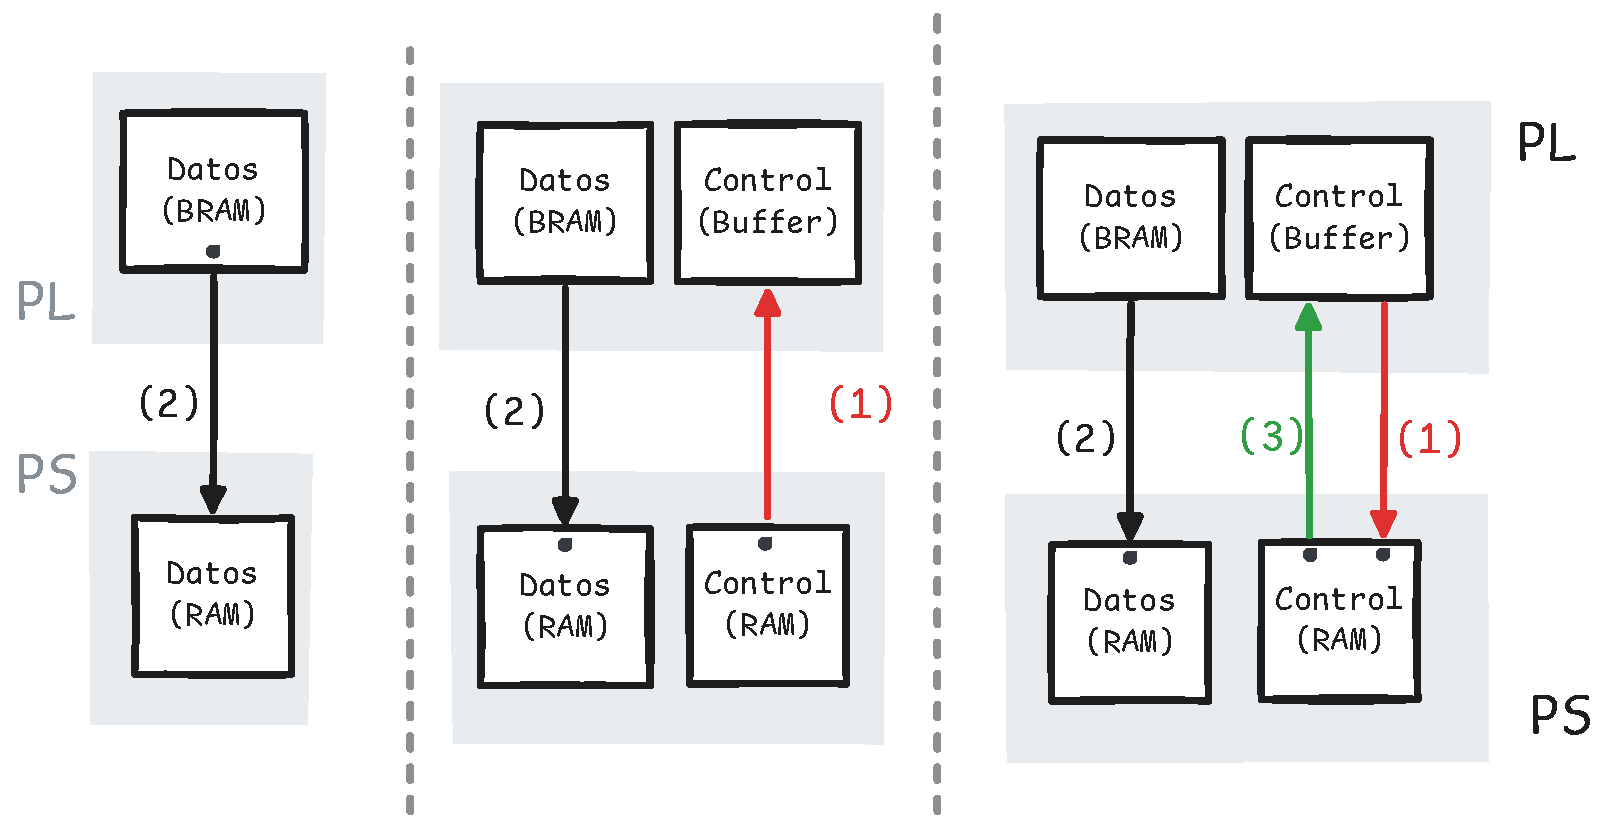
\includegraphics{cap5_tipos_control_flujo}
\caption[Esquemas de transferencia de datos entre PL y PS]{%
Esquemas de transferencia de datos entre PL y PS. (a) \emph{Fire and forget},
\emph{master}: PL. Se tiene un flujo posiblemente constante de datos. (b) Sin
\emph{feedback}, \emph{master}: PS. Esquema intermedio con validez limitada. (c) \emph{Handshake}
completo, \emph{master}: PS. \emph{Handshake} de comunicación completo; en este caso
implementado para \emph{slave} bloqueante (una única transacción en vuelo).
\label{f:intro-hw-tipos-control}}
\end{figure}

Para la comunicación de la Fig.~\ref{f:intro-hw-tipos-control}(a), del tipo
\textbf{\emph{stream}} llamada \emph{fire and forget}, se fijan las condiciones como
especificación del iniciador de trama, y el terminador puede estar especificado
o estar implícito por diseño. El receptor no tiene forma de frenar al emisor:
AXI4-Stream, por ejemplo, permite omitir la señal de vuelta \codigo{TREADY}, que
entonces se considera siempre en alto~\cite{AXIStream}.

Generalmente estas comunicaciones se realizan por el mismo \textbf{canal
físico}; la separación entre los distintos canales es lógica, porque cada uno
tiene una dirección física fija y distinta.

Es importante ver que las flechas indican el sentido de la transferencia de
datos, mientras que el punto indica quién arranca la transferencia: la
diferencia está en si se emite una \emph{request} o una \emph{response}. Por
ejemplo, en el esquema \emph{fire and forget} el \emph{master} es la PL, mientras que
en los esquemas sin \emph{feedback} y de \emph{handshake} completo el \emph{master} es el PS. Siempre
vamos a encontrar que una interfaz tiene un rol (\emph{master}/\emph{slave}) asociado, porque
es una abstracción útil: un canal bidireccional siempre puede interpretarse como
dos canales unidireccionales. Esto es extremadamente útil cuando hay una
asimetría en los roles, por ejemplo cuando un extremo genera órdenes de magnitud
más datos de los que recibe. 

Es así que se nos podría ocurrir emplear el esquema de la
Fig.~\ref{f:intro-hw-tipos-control}(b): al fin y al cabo, agregar una señal
externa del tipo \emph{enable} a un flujo constante de información es una de las
metodologías más utilizadas en DSP. En un módulo en RTL podemos trabajar con
todas las señales en todos los ciclos de reloj, pero esto no es verdad para el
PS: su vista de los registros de HW es mediante \textbf{muestreos no
necesariamente periódicos}.

El problema no es de \emph{timing}: cada lectura, por separado, es correcta. El
problema es que el PS lee la variable de control y los datos en dos
transacciones distintas, y entre una y otra la PL puede haberlos cambiado. No
tenemos la certeza de que la variable de control leída siga aplicando cuando el
PS lee los datos: es una \textbf{condición de carrera} entre productor y
consumidor, porque la lectura del par no es atómica. Este patrón, un dato y una
bandera que indica su validez, es el ejemplo con el que suele presentarse la
\textbf{consistencia} de memoria~\citecap{Nagarajan2020}{3}, que no hay que
confundir con la coherencia de las cachés de la Sec.~\ref{S:hw-cortex-a9}. La
forma más directa de arreglarlo es mantener la variable de HW fija hasta que
termine la lectura de los datos.

Esto puede resolverse de forma implícita, mediante un control que analice las
transacciones realizadas y siga de manera automática las transferencias, o de
forma explícita, en la que el PS anuncia que terminó la transferencia. Esta
última solución se presenta en la Fig.~\ref{f:intro-hw-tipos-control}(c), el
\emph{handshake} completo: el mecanismo funciona completamente con transacciones,
llamadas así porque cada transferencia de datos sigue exactamente los mismos
tres pasos, en este orden:
\begin{enumerate}
  \item El generador de los datos, en este caso dentro de la PL, presenta una
    transacción mediante un \textbf{\emph{set}} sobre un registro \textbf{\emph{valid}}. Este
    se mantiene en alto, con los datos quietos, hasta que el consumidor confirma
    la lectura.
  \item El consumidor ve el \textbf{\emph{valid}} en alto y procede a leer los datos.
  \item Cuando termina, indica al generador que puede avanzar con el siguiente
    haciendo un \emph{set} sobre la señal de \textbf{\emph{ready}}.
\end{enumerate}

AXI usa el mismo par de señales, \codigo{VALID} y \codigo{READY}, con una
diferencia: el \codigo{READY} puede subir antes que el \codigo{VALID}, y la
transferencia ocurre en el ciclo en que los dos están en
alto~\citecap{AMBAAXI}{A3}.

De manera que identificamos los esquemas \emph{fire and forget} y de
\emph{handshake} completo como los válidos; se comparan en la
Tabla~\ref{t:intro-hw-transferencias}.

\begin{table}[H]
\centering
\caption[Comparación de los esquemas de transferencia entre PL y PS]{%
Comparación de los esquemas de transferencia de datos entre la PL y el
PS.\label{t:intro-hw-transferencias}}
\begin{tabularx}{\textwidth}{|>{\raggedright\arraybackslash}p{0.2\textwidth}%
  |>{\raggedright\arraybackslash}X|>{\raggedright\arraybackslash}X%
  |>{\raggedright\arraybackslash}p{0.12\textwidth}%
  |>{\raggedright\arraybackslash}X|}
\hline \encabezado \textbf{Configuración} & \textbf{Confirmación de entrega} &
  \textbf{Control de flujo} & \textbf{Uso por control} & \textbf{Requisitos}
  \\ \hline
\emph{Handshake} completo (\emph{feedback} + \emph{ack}) & Sí & Sí (bloquea hasta \emph{match}) & 2 usos &
  Ninguno adicional: es autocontenido \\ \hline
Sin \emph{ack} (\emph{fire and forget}) & No & No (mezclado lógicamente con los datos)
  & 0 & Eventos periódicos \\ \hline
\end{tabularx}
\end{table}

A esto se le agrega la posibilidad de tener múltiples transacciones en vuelo
mediante un \emph{pipelining} de la comunicación. Esto permite mantener alto el
\emph{throughput} en las transacciones del tipo \emph{burst}. Además vamos a explorar
variantes que permiten transferencias más eficientes.

Por ejemplo, una variante del \emph{feedback} utiliza el concepto de
\textbf{créditos}~\cite[caps.~12 y 13]{Dally2004}: el receptor indica de
antemano cuánto espacio tiene disponible, de forma que el emisor puede enviar
sin esperar confirmación hasta agotar los créditos. En este proyecto los usa el
anillo de eventos que escribe en la DDR (Fig.~\ref{f:intro-hw-ring-eventos}): el
\emph{writer} sólo escribe un \emph{slot} si le quedan créditos.

\subsection{Sistemas insensibles a la latencia}
\label{S:intro-hw-latencia}

La idea primordial es la siguiente: \textbf{en un sistema real no podemos
asegurar que no se pierdan eventos}. Según la teoría de diseño insensible a la
latencia~\cite{Carloni2001}, necesitamos un bloque capaz de absorber las
diferencias temporales entre los extremos que quieren comunicarse.

El elemento fundacional de esta teoría es el \textbf{\emph{pipeline}
elástico}~\cite{Cortadella2006}, que consiste en agregar una etapa intermedia de
\emph{buffering} \textbf{controlado} que pueda amortiguar las diferencias temporales
entre producción y consumo. Generalmente se parametriza esta etapa por la
cantidad de transacciones u operaciones que puede almacenar; a este largo lo
llamamos $K$.

En la Fig.~\ref{f:intro-hw-productor-consumidor} se presenta el elemento
fundamental de estos sistemas. Tiene tres elementos: una cola y dos extremos,
uno por el que ingresan los datos, llamado generador, y otro por el que salen,
llamado consumidor.

\begin{figure}[H]
\centering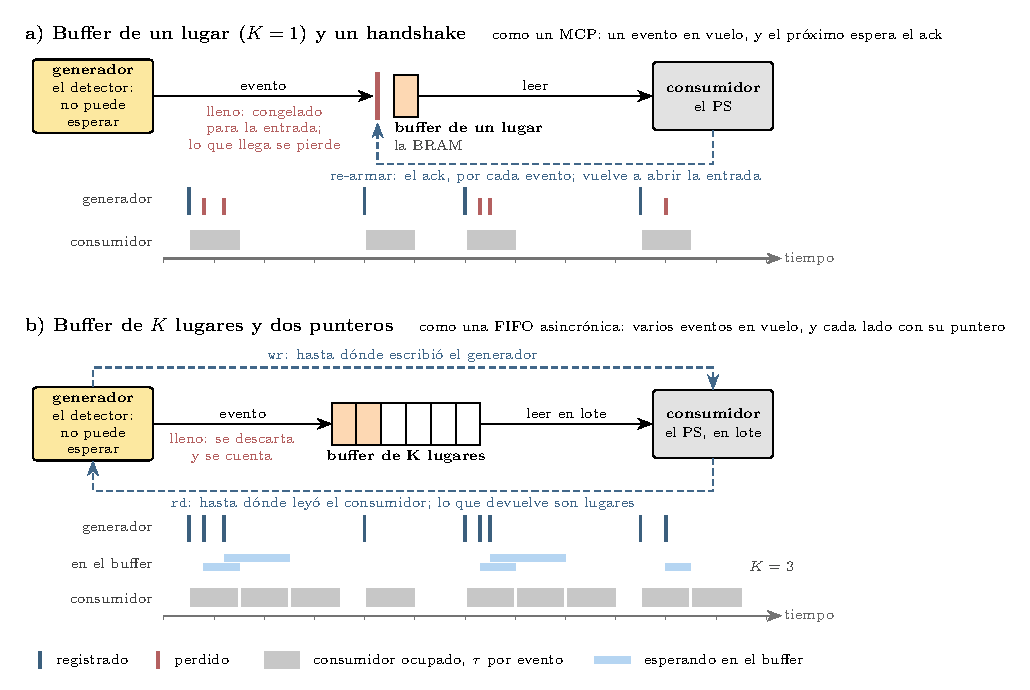
\includegraphics{cap5_productor_consumidor}
\caption[Comunicación inelástica y mediante \emph{pipeline} elástico]{%
Comparación de comunicación inelástica vs comunicación mediante \emph{pipeline}
elástico.\label{f:intro-hw-productor-consumidor}}
\end{figure}

En la Fig.~\ref{f:intro-hw-productor-consumidor}(a) se presenta un
\textbf{sistema no elástico ($K=1$)}: no hay lugar donde esperar, así que la
relación temporal entre productor y consumidor no tiene flexibilidad, y
necesitamos una transacción con la que el consumidor indica que se puede enviar
otro dato. Es lo que llamamos ``armado'', y su mecanismo es exactamente el mismo
del bus \emph{custom}: por eso esta transacción puede interpretarse como un
\codigo{ack}.

En cambio, en el elástico ($K>1$) el generador no tiene que esperar el armado
del consumidor: se desacopla el funcionamiento de cada uno. Ahora cada extremo
depende de una bandera que genera el \emph{buffer}: el generador comprueba que la
bandera \codigo{full} esté baja (todavía queda espacio) y el consumidor observa
la señal \codigo{empty}~\cite{Cummings2002}. Los buses de datos de alto
rendimiento utilizan alguna variación del \emph{pipeline} elástico; por ejemplo, las
interfaces AXI HP contienen FIFOs integradas en la interfaz
PL$\leftrightarrow$PS~\cite{UG585}.

Las tres reglas generales que necesitamos seguir son las siguientes:
\begin{enumerate}
  \item \textbf{Mayor velocidad de procesamiento que de generación}: asegurarse
    de que la metodología de transacciones tenga el \emph{throughput} necesario.
  \item Utilizar \textbf{un \emph{buffer} lo suficientemente grande}: necesitamos un
    criterio de dimensionado, que nos da la teoría de colas
    (Fig.~\ref{f:intro-hw-cola-K}).
  \item \textbf{Saber cuándo fallamos y registrarlo}: tener un mecanismo de
    registro de los tiempos de indisponibilidad o de las fallas.
\end{enumerate}

En nuestros módulos la tasa de generación es la tasa de eventos; en el caso
ideal, la cantidad de partículas detectadas en el experimento. La modifican los
falsos positivos (aumentan los disparos) y los falsos negativos (los reducen).

La tasa de consumo, en cambio, depende del \textbf{tiempo de servicio}: en este
caso, el tiempo que se tarda en pasar un lugar de la FIFO de la PL al PS. Este
largo es fijo y su comienzo depende de cuándo se empieza a ejecutar la
transacción; en el mejor caso el tiempo entre transacciones tiende a cero y
tenemos un consumidor periódico. Podríamos tener varios consumidores trabajando
en paralelo, cada uno con una interfaz AXI dedicada, pero al fin y al cabo,
mientras el \emph{throughput} sea suficiente, el cuello de botella será el dimensionado
del \emph{buffer}.

Este \emph{buffer} se suele denominar circular o anillo (\emph{ring}): no es más que
una cola del tipo FIFO cuyos punteros dan la vuelta al llegar al
final~\cite{Cummings2002}. Si medimos el largo del \emph{buffer} en eventos, es decir,
si la generación y el consumo mueven siempre el mismo largo de datos $B$, el
\emph{buffer} toma valores discretos $K$. Esto aparece en la
Fig.~\ref{f:intro-hw-ring-eventos}: la resta entre los punteros, y no su
posición, dice cuántos lugares quedan libres, y esos lugares son los créditos
del generador.

\begin{figure}[H]
\centering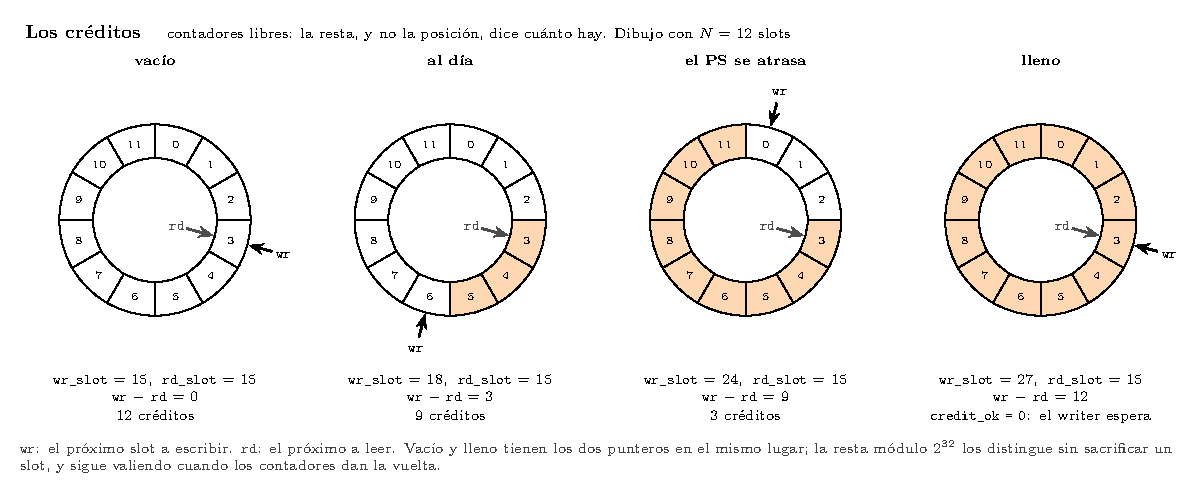
\includegraphics{cap5_ring_creditos}
\caption[Anillo de eventos y cálculo de créditos]{%
Representación de un anillo de eventos y el cálculo de créditos presentes para
cada situación.\label{f:intro-hw-ring-eventos}}
\end{figure}

Cuando no quedan créditos se detiene la sobreescritura fijando el puntero de
escritura \codigo{wr} hasta que el consumidor libere lugar; la cantidad de
ciclos que dura esto es el tiempo de indisponibilidad.

Mientras el \emph{buffer} está congelado, los eventos que llegan se pierden: es tiempo
muerto~\citecap{Knoll2010}{4}. El congelamiento resulta de que tenemos que
mantener fija una región de datos, junto con sus variables de control, hasta que
el consumidor termine de leerla.

De forma que hay dos maneras de reducir el tiempo de indisponibilidad:
\begin{enumerate}
  \item \textbf{Agrandar el \emph{buffer} de datos}: con más lugares de cola, más
    grande es la ráfaga que se puede absorber antes de quedarse sin créditos. La
    Fig.~\ref{f:intro-hw-cola-K} cuantifica cuánto rinde cada lugar.
  \item \textbf{Aumentar el \emph{throughput} de salida}:
  \begin{enumerate}
    \item Procesar varios elementos al mismo tiempo: que cada \emph{slot} se trabaje de
      forma independiente, con su propio conjunto de variables de control. Esto
      es equivalente a tener múltiples punteros de lectura \codigo{rd}, y es el
      acercamiento que empleamos para mejorar el módulo osciloscopio en la
      Sec.~\ref{S:osc-anillo-eventos}.
    \item Leer en lote: el consumidor lee muchos lugares de una vez y los
      devuelve juntos, de modo que el costo fijo de cada transacción se paga una
      vez por lote y no por evento.
  \end{enumerate}
\end{enumerate}

Con un análisis de teoría de colas~\cite{Kendall1953,Gross2008} podemos llegar
a resultados sobre la fracción de eventos perdidos con un productor poissoniano
y un consumidor de tiempo de servicio fijo, que se presentan en la
Fig.~\ref{f:intro-hw-cola-K}. Para $K=1$ no hay cola: si llega un evento con el
consumidor ocupado, se pierde. Con carga baja, $\rho \ll 1$, la pérdida pasa de
$\approx\rho$ a $\approx\rho^K/K!$: cada lugar de cola (aumentar $K$) la baja en
un orden de magnitud o más. Por encima, el consumidor no da abasto en promedio,
ninguna cola alcanza y todas las curvas tienden a $1 - 1/\rho$: el \emph{buffer}
absorbe ráfagas, no un exceso de tasa.

\begin{figure}[H]
\centering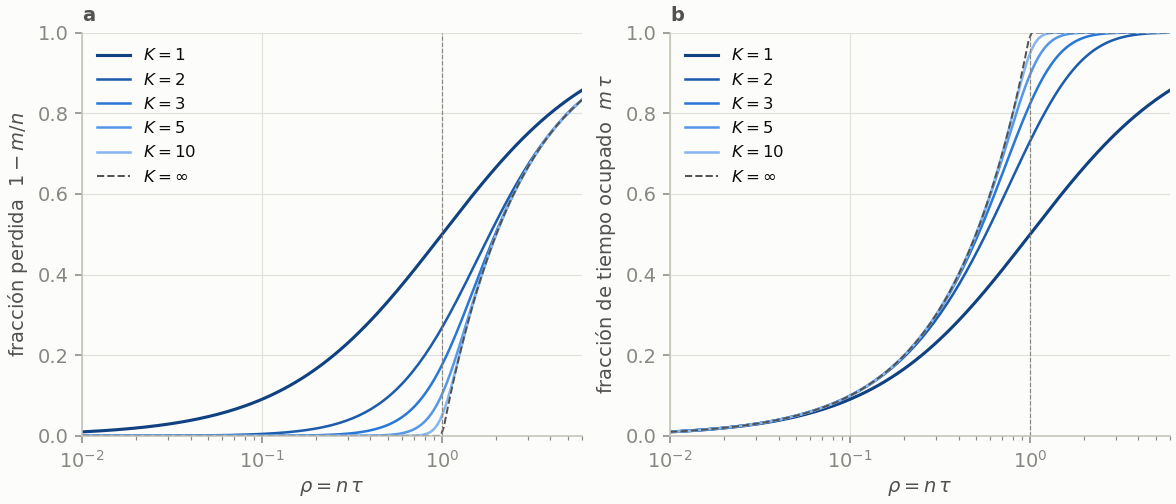
\includegraphics{cap5_cola_K}
\caption[Fracción de eventos perdidos según el largo de cola]{%
(a) Fracción de eventos perdidos en función de la carga $\rho = n\tau$ (tasa
incidente por tiempo de servicio), con arribos Poisson y servicio fijo, para
distintos largos de cola $K$. (b) Fracción del tiempo con el consumidor
ocupado.\label{f:intro-hw-cola-K}}
\end{figure}


\subsubsection{Pérdidas de transacciones por \emph{back-pressure}}
\label{S:intro-hw-back-pressure}

En una red de procesamiento \emph{feed-forward}, es decir, sin ciclos, tenemos
que poner criterios sobre el funcionamiento de los descartes en las ramas
paralelas. En la Fig.~\ref{f:intro-hw-perdida-back-pressure} se presentan los
tres casos típicos. El primero (a) es una cadena estrictamente lineal: los
descartes totales son la suma directa de los descartes de cada etapa. En cambio
(b) y (c) contienen ramas; en (b) las ramas son mutuamente excluyentes, así que
la suma sigue valiendo.

\begin{figure}[H]
\centering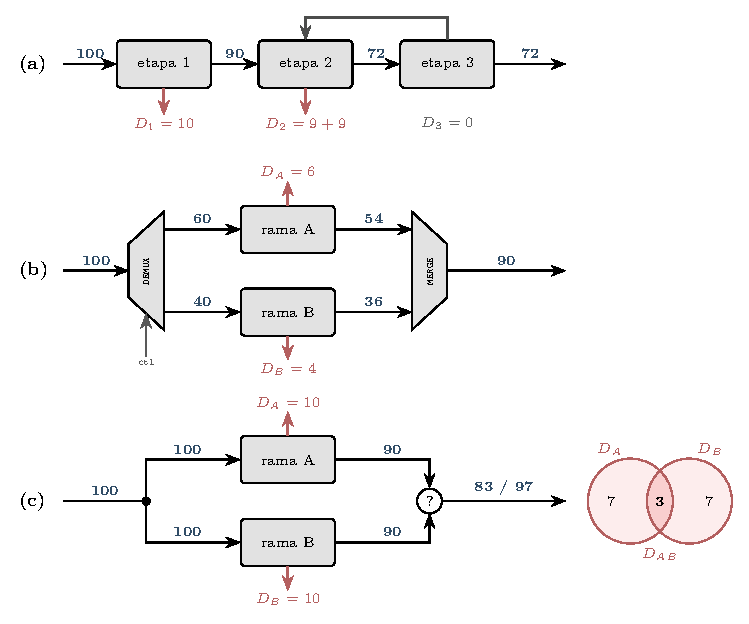
\includegraphics{cap5_perdida_back_pressure}
\caption[Suma de pérdidas en una red \emph{feed-forward}]{%
Cómo se suman las pérdidas en una red de procesamiento \emph{feed-forward}, con
100 eventos de entrada de ejemplo. (a) Cadena lineal: la pérdida total es la
suma de lo que descarta cada etapa. (b) Ramas exclusivas: ningún evento está en
las dos ramas y la suma sigue valiendo. (c) Ramas no exclusivas: la pérdida
depende de qué cuenta como sobrevivir, y la suma de los contadores cuenta dos
veces los eventos perdidos en las dos
ramas.\label{f:intro-hw-perdida-back-pressure}}
\end{figure}

El dilema aparece con dos ramas que no son mutuamente excluyentes (c), porque el
criterio de descarte sale de la lógica local de cada bloque. En este ejemplo
podríamos tener como criterio que un evento se pierda sólo si ambas ramas fallan
simultáneamente, y entonces la suma de los 10 descartes que reporta cada bloque
no refleja el valor final. Una forma de arreglarlo es diseñar la red de forma
que los elementos de las ramas paralelas no puedan descartar, sino sólo
bloquear la entrada hasta la etapa anterior al punto donde se separan las ramas,
y contar los descartes en la sección secuencial. Esto significa que no todos los
bloques descartan: algunos \textbf{bloquean} el flujo de datos, y ese bloqueo que
se propaga hacia atrás es la \emph{back-pressure}
(contrapresión)~\cite[caps.~12 y 13]{Dally2004}.

Que un bloque descarte o bloquee depende del esquema de comunicación de cada
etapa. Por ejemplo, un ADC trabaja en modo \emph{fire and forget}: su salida no
tiene control de flujo ni confirmación de llegada, mientras que los elementos
dentro de la cadena sí los tienen. La consecuencia a nivel de bloque es que
donde la comunicación es unidireccional, es decir, donde \textbf{no vemos flecha
de vuelta}, el sistema puede descartar.

Esto quiere decir que los bloques no necesariamente avanzan en todos los ciclos
de reloj: como los eventos llegan a una tasa mucho menor que la del reloj, la
cadena no necesita procesar uno por ciclo, y eso nos deja implementar mecanismos
de control más complejos.

Lo que importa es cómo se traduce el bloqueo en descartes
(Fig.~\ref{f:intro-hw-etapas-descartes}): si la \emph{back-pressure} llega hasta
un bloque con una entrada ininterrumpida, como un ADC, tenemos un descarte.

\begin{figure}[H]
\centering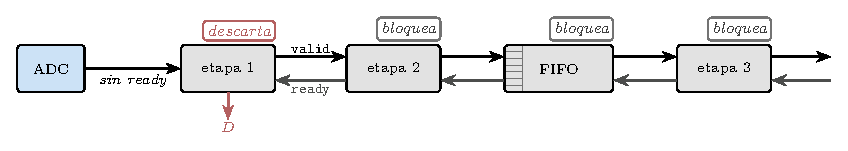
\includegraphics{cap5_etapas_vs_descartes}
\caption[Descartes y bloqueos de las etapas de procesamiento]{%
Descartes y bloqueos de las etapas de
procesamiento.\label{f:intro-hw-etapas-descartes}}
\end{figure}

%==============================================================================
\section{Bus \emph{custom} de RedPitaya}
\label{S:intro-hw-bus-custom}

El bus \emph{custom} de Red Pitaya~\cite{RedPitayaFPGA} puede emplear cualquiera de los
mecanismos de transferencia explicados en la Sec.~\ref{S:intro-hw-transferencia}
en los que la PL funciona como \emph{slave}. Cada operación sobre este bus representa
una flecha de la Fig.~\ref{f:intro-hw-tipos-control}. En todos los módulos que
usan este bus utilizamos el esquema de \emph{handshake} completo.

Los elementos conectados a él tienen que implementar la decodificación de
direcciones y respetar un ordenamiento en el acceso: como hay un único
\codigo{ack}, todos los módulos deben \textbf{turnarse la utilización del bus}.
En la Fig.~\ref{f:intro-hw-fsm-bus} se presenta la máquina de estados que
\textbf{sigue el bus} \emph{custom} de Red Pitaya. A esta secuencia de pasos se la suele
denominar \textbf{contrato}, porque la FSM no se implementa explícitamente: se
diseñan \emph{slaves} y \emph{masters} que cumplen sólo lo que se le exige a cada extremo.
Esto se refleja en optimizaciones, simplificaciones y consideraciones
importantes para su diseño y uso. Los pasos son:
\begin{enumerate}
  \item \textbf{Reposo}: el bus está libre, con \codigo{wen} y \codigo{ren}
    en~0.
  \item \textbf{Pedido}: el maestro pone \codigo{addr} (y \codigo{wdata}, si es
    escritura) y levanta \codigo{wen} o \codigo{ren}. El esclavo ejecuta la
    escritura, o lanza la lectura, una sola vez, con un estrobo de un ciclo.
  \item \textbf{Espera}: \codigo{wen}/\codigo{ren} siguen en alto y
    \codigo{addr} y \codigo{wdata} quedan quietos hasta el \codigo{ack}. Del
    lado del esclavo no hay \emph{timeout}: si el \codigo{ack} no llega, el \emph{slot} se
    queda en este estado. El maestro sí tiene uno, que se describe en la
    Sec.~\ref{S:intro-hw-modos-falla}.
  \item \textbf{\emph{Acknowledge}}: el esclavo levanta \codigo{ack}, con
    \codigo{rdata} ya registrado en el caso de una lectura. El maestro lo ve,
    baja \codigo{wen}/\codigo{ren}, y el bus vuelve a reposo.
\end{enumerate}

\begin{figure}[H]
\centering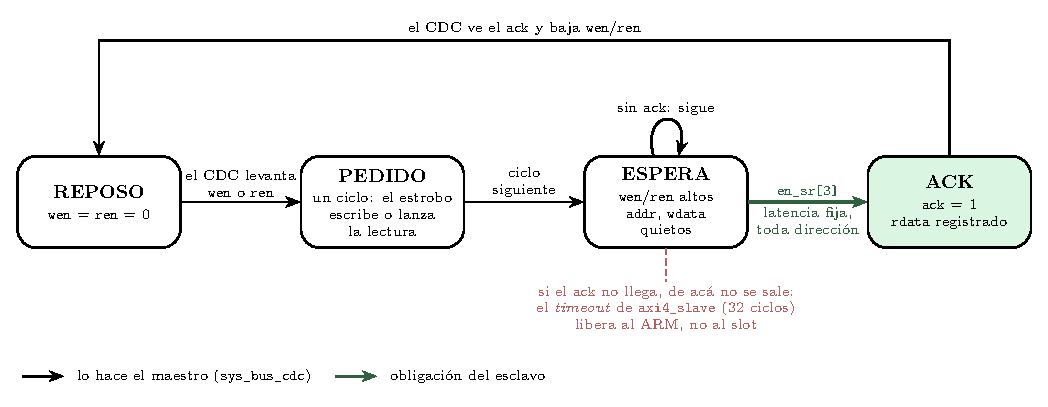
\includegraphics{cap5_contrato_sys_bus}
\caption[Contrato del bus \emph{custom} de Red Pitaya]{%
Diagrama del bus \emph{custom} de RedPitaya. Contiene cuatro
estados.\label{f:intro-hw-fsm-bus}}
\end{figure}

La única obligación del esclavo es la del paso~4: responder a toda dirección de
su \emph{slot} (que la \emph{request} sea para él), mapeada o no, con latencia fija.

\subsection{Rendimiento del bus}
\label{S:intro-hw-rendimiento-bus}

La Fig.~\ref{f:intro-hw-camino-bus} presenta las 4 etapas de una lectura o
escritura de 32 bits por el bus \emph{custom} de Red Pitaya a un \emph{slave} genérico.

\begin{figure}[H]
\centering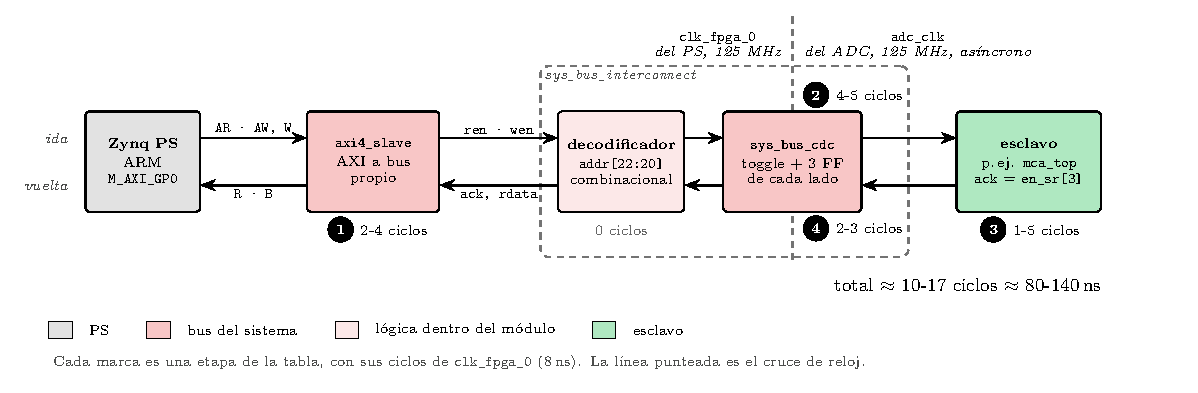
\includegraphics{cap5_latencia_sys_bus}
\caption[Camino de una transferencia por el bus \emph{custom}]{%
Flujo de comunicación para una transferencia PS$\rightarrow$\emph{slave} de la PL
mediante el bus \emph{custom}.\label{f:intro-hw-camino-bus}}
\end{figure}

Arrancamos con el camino PS$\rightarrow$PL, que pasa por el
\codigo{axi4\_slave} con una latencia de 2 a 4 ciclos según la transacción: 2
para la lectura y hasta 4 para la escritura, según el orden de llegada de la
dirección y los datos. Los cruces \codigo{clk\_fpga0} $\rightarrow$
\codigo{adc\_clk} (paso~2) y \codigo{adc\_clk} $\rightarrow$
\codigo{clk\_fpga0} (paso~4) usan el mismo CDC, un \emph{handshake} por
\emph{toggle}~\cite{Cummings2008} de 4 a 5 ciclos. La variación se debe a que depende
de la diferencia de fase entre los relojes.

En la Tabla~\ref{t:intro-hw-rendimiento-bus} se describe cada uno de estos pasos
y se calcula la latencia total de la comunicación. Los valores de cada etapa son
los del diseño de Red Pitaya, y los del CDC no conviene achicarlos: para relojes
asincrónicos, sin relación de frecuencia fraccional, la tasa de fallas por
metaestabilidad crece de forma exponencial al reducir el tiempo de
sincronización~\cite{Ginosar2011}. Para el esclavo se consideró uno genérico,
con un tiempo de respuesta de hasta 5 ciclos.

Cuando ambos dominios tienen la misma frecuencia, las sincronizaciones de ida y
de vuelta suelen ser instancias de un mismo módulo, y por eso los ciclos
requeridos en ambos trayectos son iguales. Cuando la relación de frecuencias es
mayor, $f_\text{max} > 2f_\text{min}$, podríamos utilizar otros esquemas de
sincronización, en los que se diferencian los caminos \emph{fast-to-slow} y
\emph{slow-to-fast}~\cite{Cummings2008}.

\begin{table}[H]
\centering
\caption[Latencia de una transacción del bus \emph{custom}]{%
Estimados de latencia por etapa y total para una transacción del bus \emph{custom} de
RedPitaya.\label{t:intro-hw-rendimiento-bus}}
\begin{tabular}{|c|l|l|}
\hline \encabezado \textbf{\#} & \textbf{Etapa} & \textbf{Ciclos requeridos}
  \\ \hline
1 & AXI + \codigo{axi4\_slave} & 2--4 \\ \hline
2 & CDC ida (\emph{toggle} + 2--3 \emph{flops}) & 4--5 \\ \hline
3 & Esclavo & 1--5 \\ \hline
4 & CDC vuelta & 4--5 \\ \hline
  & \textbf{Total} & \textbf{$\sim$12--20} $\approx$
    \qtyrange{100}{160}{\nano\second} \\ \hline
\end{tabular}
\end{table}

Estas latencias provienen de que los dos extremos no comparten reloj. Es una
cuestión de \emph{trade-off}: no vale la pena quitar el problema de raíz si sincronizar
los relojes es tan costoso en HW y podemos diseñar sistemas que compensen
parcialmente sus efectos, como el \emph{pipeline} elástico.

\subsection{\emph{Waveforms} de transacciones por \texttt{axi4\_slave}}
\label{S:intro-hw-waveforms-axi}

En la Fig.~\ref{f:intro-hw-escritura} presentamos una \emph{waveform} de una
transferencia de escritura del parámetro \codigo{cfg\_amp\_max} (de dirección
\codigo{0x4070\_0034}) obtenida por simulación. Se tienen los siguientes pasos:
\begin{enumerate}
  \item \emph{Master}: pone los valores de \codigo{addr} y \codigo{wdata} y levanta
    \codigo{wen} (ciclo~2).
  \item \emph{Slave}: ve el cambio en \codigo{wen} (\qty{35}{\nano\second} después) y
    genera una operación de un ciclo (\textbf{estrobo}); en el flanco siguiente
    \codigo{cfg\_amp\_max} toma el valor de \codigo{wdata} (ciclo~8).
  \item \emph{Slave}: con la latencia fija del módulo, sube \codigo{sys\_ack}
    (ciclo~12).
  \item \emph{Master}: ve el \codigo{ack} ya sincronizado (\qty{96}{\nano\second}
    después de iniciar la transacción) y baja \codigo{wen}, completando la
    transacción.
\end{enumerate}

En la lectura se mantienen los roles \emph{master}/\emph{slave} y la transacción es casi
idéntica; se puede ver en la Fig.~\ref{f:intro-hw-lectura}. Sus diferencias son
las siguientes:
\begin{enumerate}
  \item \emph{Master}: fija únicamente \codigo{addr} (no pone \codigo{wdata}) y
    levanta \codigo{ren} en vez de \codigo{wen} (ciclo~2).
  \item \emph{Slave}: el valor de \codigo{rdata} hay que tomarlo cuando \codigo{ack}
    está en alto (ciclo~17).
\end{enumerate}

% Las dos waveforms son muy anchas (20 x 5 pulgadas): van juntas en una página
% apaisada, cada una con su número y epígrafe.
\begin{figuraapaisada}
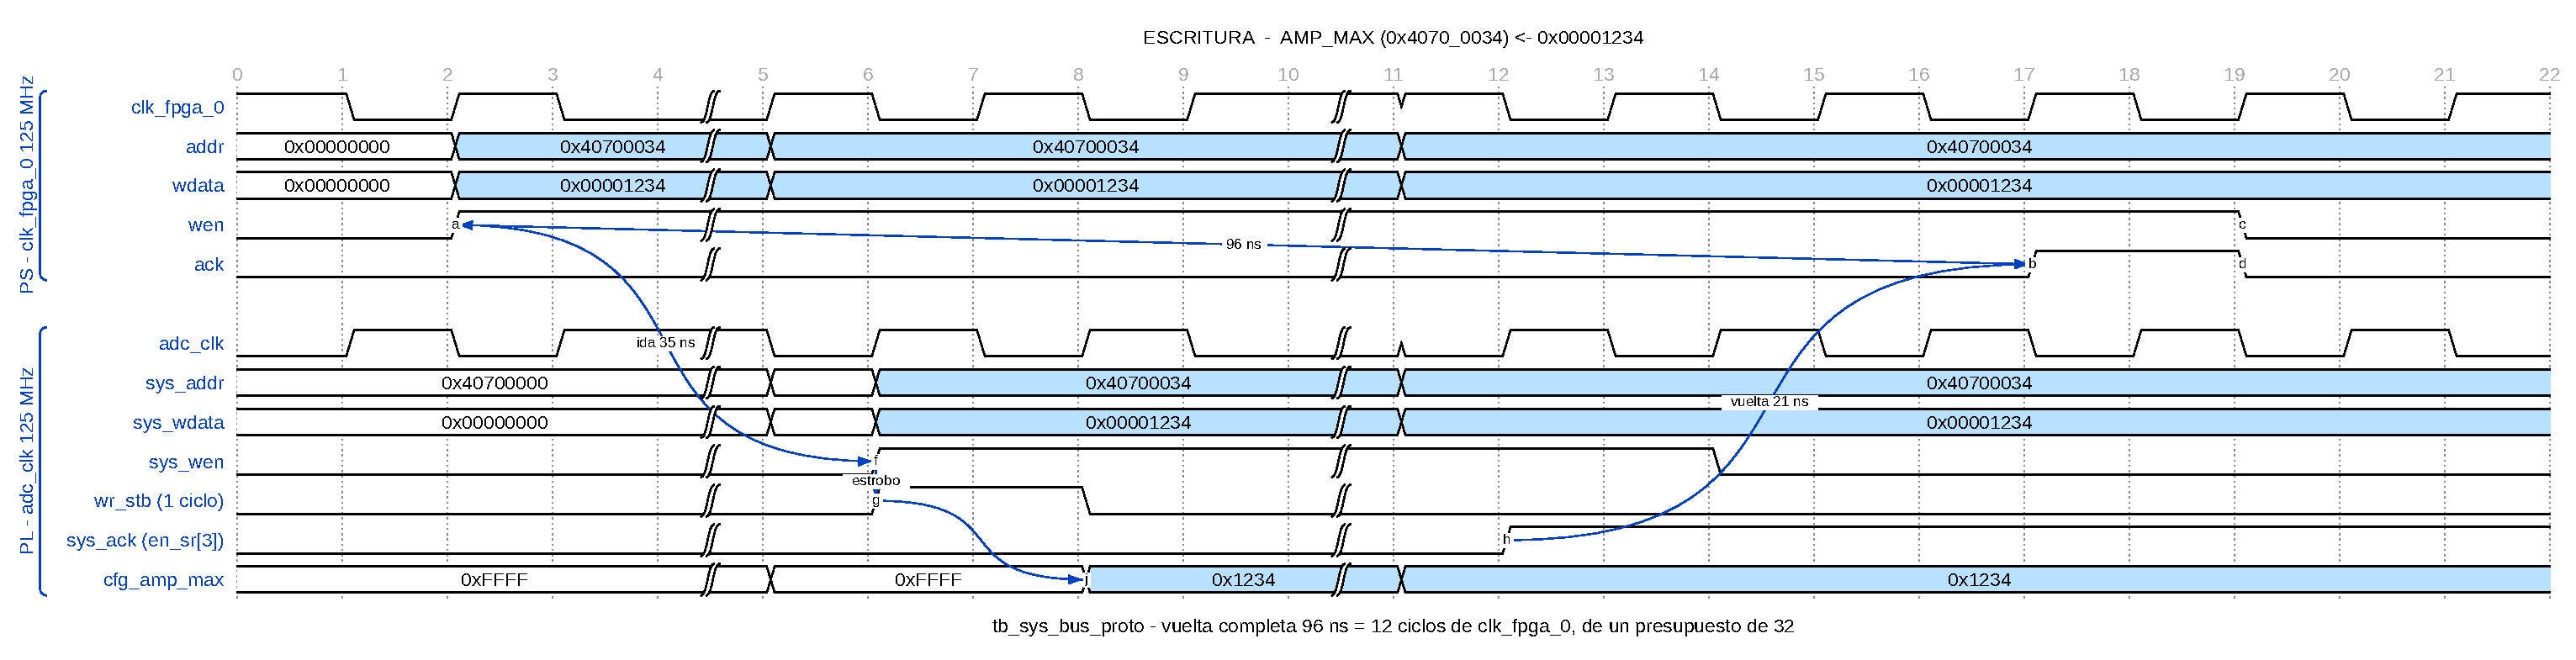
\includegraphics[height=0.4\textwidth]{cap5_bus_escritura}
\caption[\emph{Waveform} simulada de una escritura por el bus \emph{custom}]{%
\emph{Waveform} simulada de la transacción de escritura al registro
\codigo{AMP\_MAX}, de dirección \codigo{0x4070\_0034}, con el valor
\codigo{0x1234}.\label{f:intro-hw-escritura}}

\vspace{2\baselineskip}
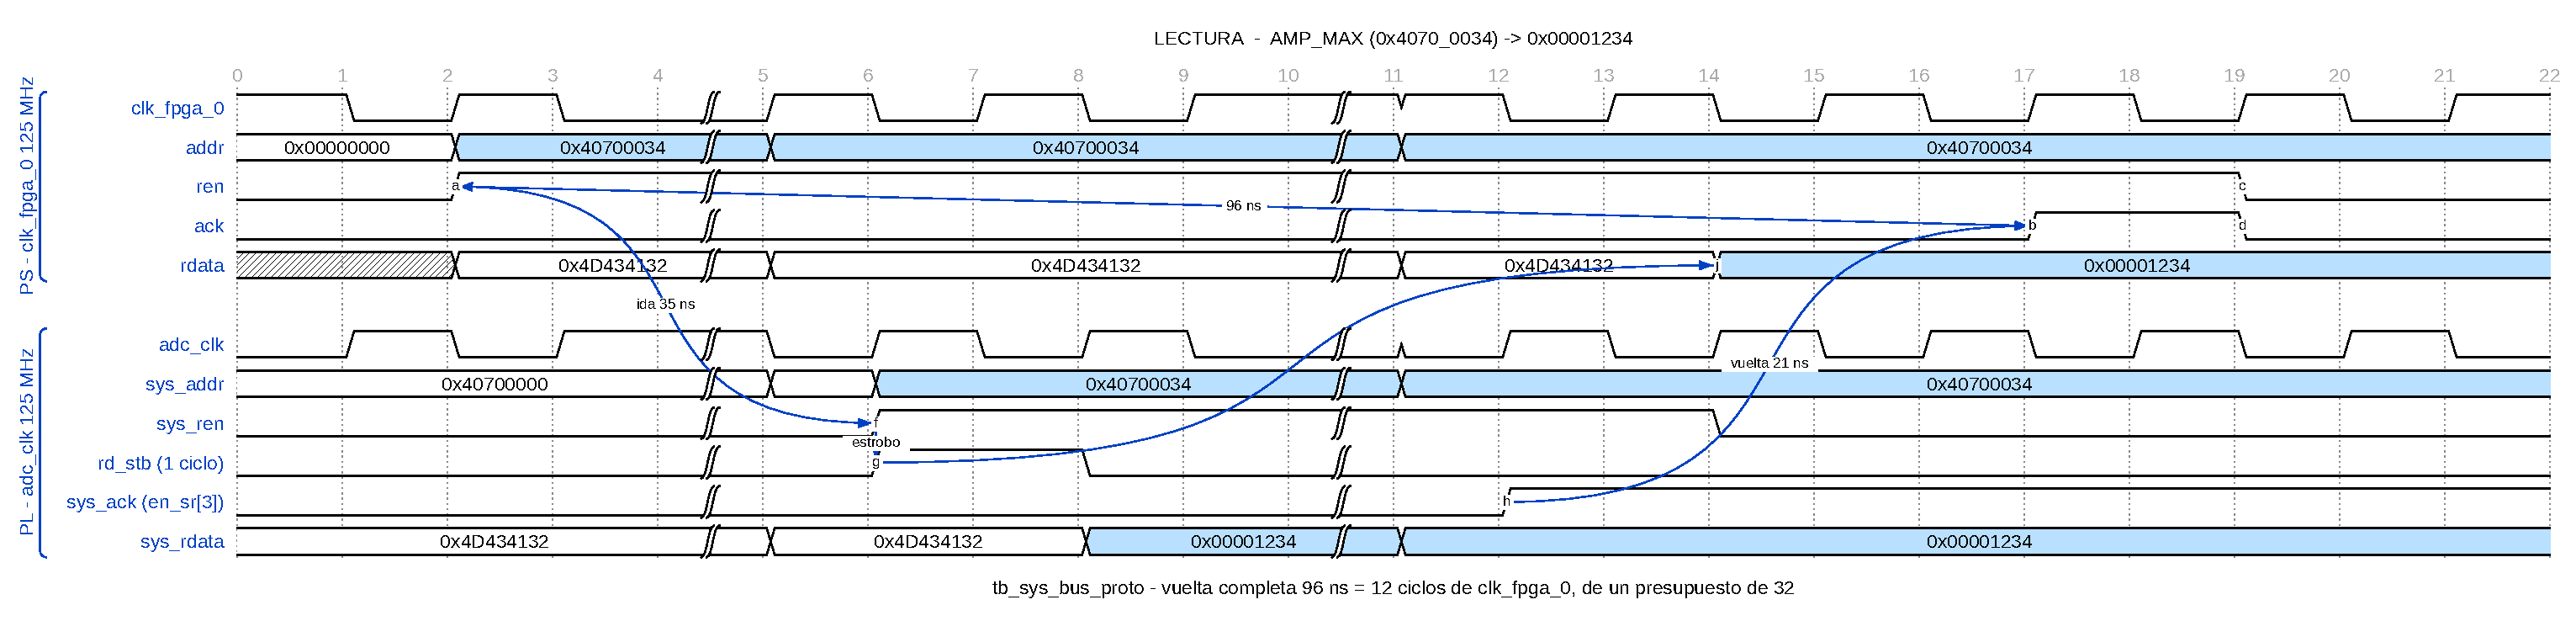
\includegraphics[height=0.4\textwidth]{cap5_bus_lectura}
\caption[\emph{Waveform} simulada de una lectura por el bus \emph{custom}]{%
\emph{Waveform} simulada de la transacción de lectura al registro \codigo{AMP\_MAX},
de dirección \codigo{0x4070\_0034}.\label{f:intro-hw-lectura}}
\end{figuraapaisada}

\subsection{Mapa de registros}
\label{S:intro-hw-mapa-registros}

Es una tabla en la que asociamos \textbf{direcciones físicas y permisos de
acceso} a los registros de control y de estado de un módulo. Los módulos
empleados tienen dos clases de parámetros: los compartidos y los específicos de
cada \emph{stream} de datos. Lo que suele hacerse es colocar las configuraciones
compartidas en la base de la estructura y después la configuración de cada uno
de los bloques, de forma individual.

Cada módulo tiene \textbf{su mapa de registros local}, que en la etapa de
integración se ubica en el mapa de memoria del sistema mediante un \emph{offset} fijo.
Esto simplifica el SW, porque entre las configuraciones de los bloques hay un
salto fijo, llamado \textbf{\emph{stride}}: las estructuras quedan compactas y se
representan fácilmente con \emph{structs} de C.

En la Fig.~\ref{f:intro-hw-mapa-registros} se presenta, de izquierda a derecha,
el mapa de direcciones físicas de la PL, que tiene que coincidir con el que ve el
PS~\cite{UG585}. Consta de 8 regiones de 1~MB cada una. El segundo \emph{slot} es el
mapa de direcciones del módulo osciloscopio, que repite las direcciones previas
(el mapa \emph{legacy}) para que la API precompilada de Red Pitaya siga siendo
compatible.

\begin{figure}[H]
\centering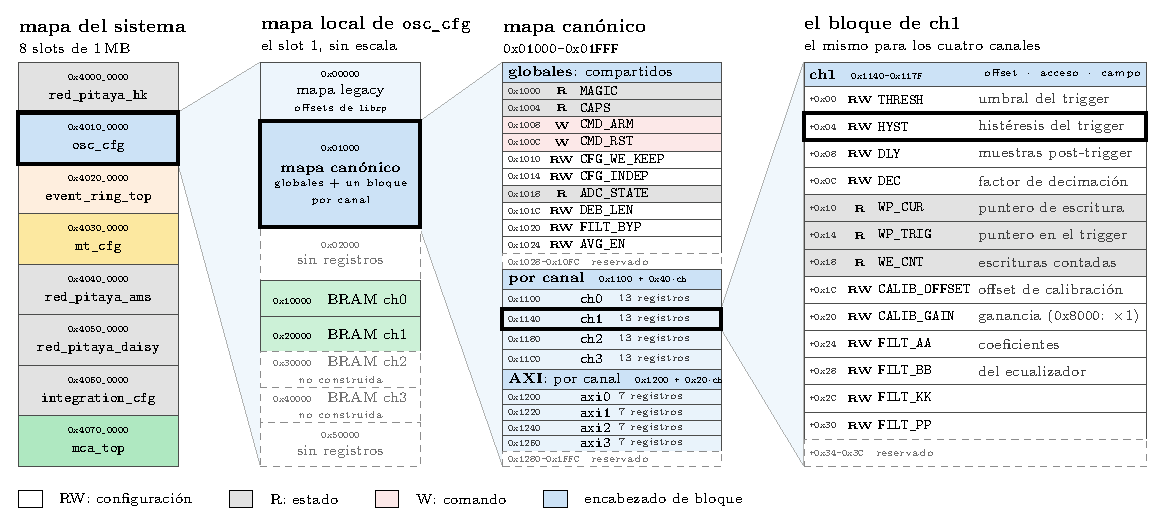
\includegraphics{cap5_mapa_registros_osc}
\caption[Cuatro escalas del mapa de registros]{%
Cuatro escalas del mapa de registros. (a) Nivel sistema. (b) Nivel módulo:
contiene datos (ver BRAM presente). (c) Nivel configuración de módulo. (d) Nivel
configuración de un canal.\label{f:intro-hw-mapa-registros}}
\end{figure}

Al realizar una transacción, el sistema analiza los prefijos de la dirección
para averiguar cómo rutear la transferencia: por ejemplo, como la dirección
arranca con \codigo{b0100000}, el PS sabe de entrada que le corresponde la
interfaz AXI GP0~\cite{UG585}. Después la dirección la lee el
\codigo{sys\_bus\_interconnect}, que decodifica el \emph{slot} dentro del mapa de
memoria global y redirige la transacción al módulo de sincronización asociado.
En la Fig.~\ref{f:intro-hw-calculo-direccion} se pueden ver las distintas capas
de direccionamiento para la dirección \codigo{0x4010\_1144}, que pertenece al
registro \codigo{HYST} del canal~1 del \emph{slot}~1 (OSC).

\begin{figure}[H]
\centering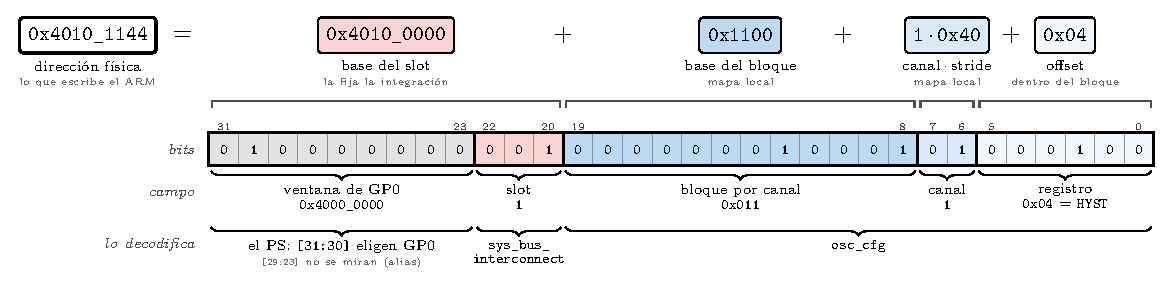
\includegraphics{cap5_calculo_direccion_osc}
\caption[Enrutamiento de una dirección según regiones de memoria]{%
Ejemplo de enrutamiento según regiones de
memoria.\label{f:intro-hw-calculo-direccion}}
\end{figure}

Es interesante notar que la dirección queda asociada a la interfaz GP0. Si la PL
tuviera el mismo \emph{slave} conectado también a la otra interfaz maestra del PS, la
GP1, podríamos asociar \textbf{el mismo registro a otra región de memoria} y
acceder a él por ese otro camino de datos. Las interfaces HP no sirven para
esto: en ellas el \emph{master} es la PL.

\subsection{Modos de falla del bus interno}
\label{S:intro-hw-modos-falla}

A continuación comentamos las formas de llevar el sistema a un estado erróneo.
Son fallas que exceden al módulo que las provoca: aparecen en la interacción
entre el PS, el \codigo{axi4\_slave} y el \emph{slave}.
\begin{enumerate}
  \item \textbf{\emph{Slave} que no hace \codigo{ack}}: los \emph{slaves} comparten el recurso
    que representa el bus. Si un \emph{slave} no hace \codigo{ack}, su \emph{slot} queda en el
    estado de espera de la Fig.~\ref{f:intro-hw-fsm-bus} y el CDC de ese \emph{slot}
    queda desincronizado: es un \textbf{\emph{deadlock}} latente del \emph{slot}, y las
    transacciones siguientes a ese \emph{slot} salen corruptas. El PS no se cuelga
    porque el \codigo{axi4\_slave} tiene un \emph{timeout}: a los 32 ciclos
    fabrica el \codigo{ack} y responde con error
    (\codigo{SLVERR})~\cite{AMBAAXI,RedPitayaFPGA}, que el ARM recibe como un
    \emph{external abort}. Por eso un \emph{slave} tiene que hacer \codigo{ack} de toda
    dirección de su \emph{slot}, mapeada o no; el \emph{timeout} es una red de seguridad, no
    parte del contrato.
  \item \textbf{Ráfagas y anchos incorrectos}: el \codigo{axi4\_slave} que
    conecta el bus \emph{custom} implementa una versión reducida de AXI: no acepta
    transferencias en ráfaga ni accesos anchos, sólo \codigo{LEN = 0} y
    \codigo{SIZE} de 2 o 4 bytes~\cite{AMBAAXI}. Cualquier otra transacción la
    rechaza con \codigo{SLVERR} sin que llegue al \emph{slave}. Esto es importante
    porque limita las instrucciones que podemos usar desde el PS; se expande
    este tema en la Sec.~\ref{S:sw-modos-fallo}.
\end{enumerate}

Es un buen ejemplo de por qué conviene conocer el modelo de memoria del
procesador~\cite{DDI0406C}: el \emph{bug} no está ni en el RTL ni en el código Python,
sino en la interacción entre lo que la ISA permite emitir y lo que el esclavo
acepta recibir.

\subsection{Módulo de configuración}
\label{S:intro-hw-modulo-config}

Los módulos implementados tienen un submódulo de configuración, por ejemplo
\codigo{mt\_cfg}, \codigo{osc\_cfg} e \codigo{integration\_cfg}; en el MCA la
misma lógica está dentro de \codigo{mca\_top}. Es el que \textbf{implementa el
acceso por un mapa de registros} y la transferencia al bus \textbf{\emph{custom}}.
Todos repiten la misma estructura; en la Fig.~\ref{f:intro-hw-panorama-cfg} se
presenta una versión tipo plantilla. Los bloques en gris son plantillas que
contienen los elementos \emph{ad hoc} que requiera el diseño:
\begin{itemize}
  \item \textbf{Comandos}: generalmente generan señales de un ciclo de reloj que
    arrancan un comando, representado por una FSM en el módulo.
  \item \textbf{Registros de configuración}: generalmente son señales lentas.
  \item \textbf{Identificación}: un número fijo en el HW con el que se puede
    diagnosticar rápidamente si la carga del \emph{bitstream} en la placa fue exitosa;
    se lo utiliza para identificar el módulo y comprobar la versión.
  \item \textbf{Lógica}: el resto de los elementos que no entran en las
    categorías previas, por ejemplo los registros tipo \emph{snapshot}.
\end{itemize}
Los bloques en rojo claro representan bloques de RTL fijos para todos los
módulos de configuración:
\begin{itemize}
  \item \textbf{Escritura}: un decodificador de dirección traduce el \emph{offset}
    (\codigo{sys\_addr[19:0]}) en la habilitación del registro que le
    corresponde, y ese registro copia su campo de \codigo{sys\_wdata}.
  \item \textbf{Estrobo}: \codigo{sys\_wen} queda alto hasta el \codigo{ack},
    unos 5 ciclos. El estrobo lo convierte en un pulso de un ciclo
    (\codigo{wr\_stb = sys\_wen \&\& !en\_sr[0]}), para que cada
    \textbf{escritura se ejecute una sola vez}.
  \item \textbf{\emph{Ack}}: sale de un registro de desplazamiento sobre
    \codigo{sys\_en = sys\_wen | sys\_ren}, con latencia fija y para cualquier
    dirección, mapeada o no. \codigo{sys\_err} vale siempre~0.
  \item \textbf{Lectura}: un multiplexor controlado por la misma dirección elige
    qué va a \codigo{sys\_rdata}. Puede ser el valor escrito, el estado y los
    contadores de la región, la identificación o, en los módulos con memoria,
    una ventana de BRAM o de histograma. Las direcciones no mapeadas leen~0. La
    salida del multiplexor pasa por un registro: \codigo{sys\_rdata} cruza al
    dominio de reloj del PS sin sincronizador~\cite{Cummings2008} y con menos de
    \qty{1}{\nano\second} de margen, así que no puede llevar lógica
    combinacional.
\end{itemize}

\begin{figure}[H]
\centering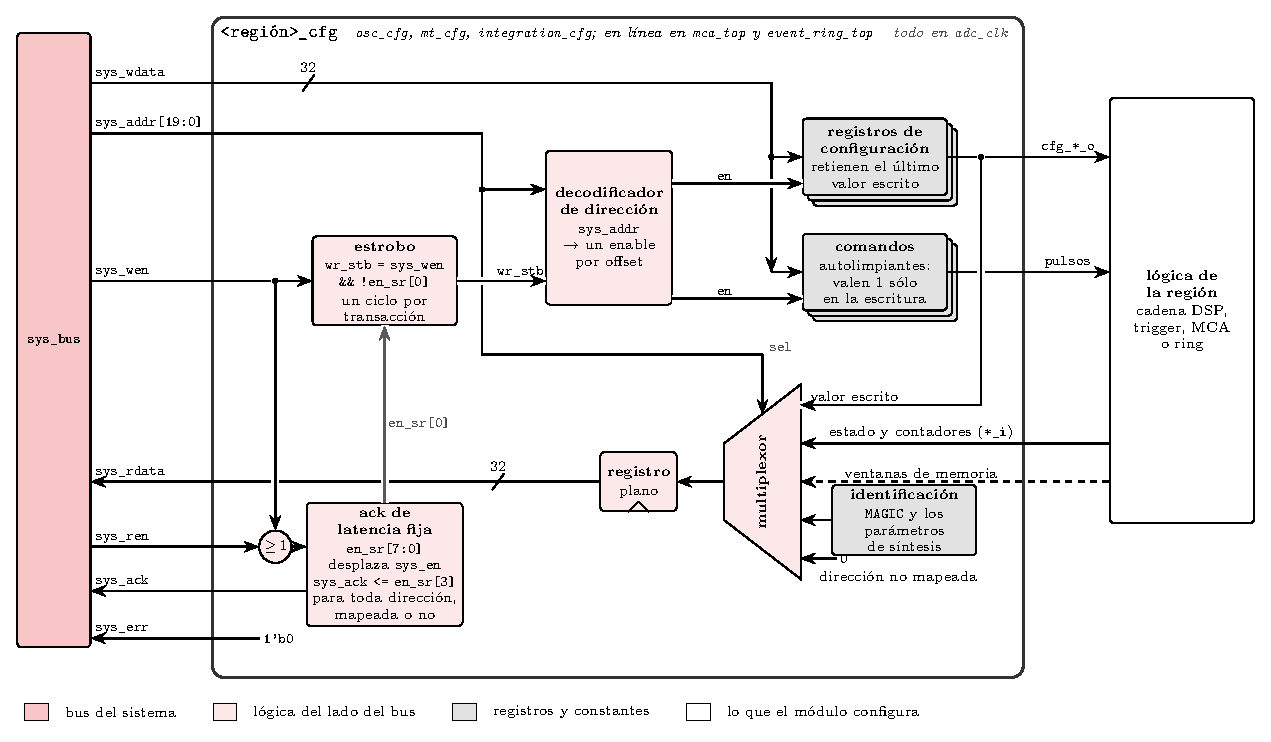
\includegraphics{cap5_panorama_modulo_cfg}
\caption[Plantilla del módulo de configuración]{%
\emph{Template} del módulo de configuración, incluye conexión al bus \emph{custom} de
RedPitaya.\label{f:intro-hw-panorama-cfg}}
\end{figure}

Ahora que terminamos de ver los temas generales del diseño de HW, tenemos que
ver cómo comprobamos su funcionamiento: este es el dominio de la verificación.

%==============================================================================
\section{Verificación}
\label{S:intro-hw-verificacion}

Quien haya trabajado en diseño de HW sabe lo exhaustiva que puede volverse la
verificación previa a la síntesis: se lleva una fracción importante del tiempo
de los proyectos de FPGA~\cite{Foster2022}. A nuestro entender, se debe
principalmente a los siguientes elementos:
\begin{itemize}
  \item No tenemos herramientas de \emph{debug} intrínsecas al hardware realizado:
  \begin{itemize}
    \item A diferencia del SW, en el que tenemos un \emph{debugger} para diagnosticar
      los errores en tiempo de ejecución, en HW no tenemos estas capacidades a
      menos que exportemos las señales hacia afuera, por ejemplo con un
      analizador lógico integrado en la FPGA, que consume recursos y sólo ve las
      señales que elegimos antes de sintetizar.
  \end{itemize}
  \item El \textbf{espacio de entradas} de un módulo puede ser
    \textbf{arbitrariamente grande}, y su espacio de estados crece de forma
    exponencial con la cantidad de registros.
  \begin{itemize}
    \item En cada ciclo todas las entradas tienen un valor, así que hay que
      analizar el efecto de todas las entradas del módulo en todos los ciclos.
    \item Acordémonos de que el punto más fuerte de estas plataformas es el
      paralelismo: muchas cosas pasan en el mismo ciclo, y las combinaciones de
      eventos simultáneos se multiplican.
  \end{itemize}
  \item Trabajamos en escalas temporales muy distintas:
  \begin{itemize}
    \item Como ejemplo, nuestra placa trabaja a \qty{125}{\mega\hertz}: un
      segundo de funcionamiento son $1,25\cdot10^{8}$ ciclos. Una falla que
      aparece una vez cada millón de ciclos se ve en la placa en milisegundos,
      pero en simulación exige corridas larguísimas o un estímulo dirigido que
      la provoque.
  \end{itemize}
\end{itemize}

\subsection{Técnicas de verificación}
\label{S:intro-hw-tecnicas}

Tenemos una variedad de técnicas y herramientas para verificar tanto la
funcionalidad como la factibilidad; en la Tabla~\ref{t:intro-hw-tecnicas}
aparece qué detecta cada una.

\begin{table}[H]
\centering
\caption[Qué detecta cada técnica de verificación]{%
Qué detecta cada una de las técnicas de verificación más empleadas.
$^{*}$Sólo para las propiedades que se escriban.\label{t:intro-hw-tecnicas}}
\begin{tabularx}{\textwidth}{|X|c|c|c|c|}
\hline \encabezado & \textbf{Lint} & \textbf{STA} &
  \textbf{\emph{Golden model} + \emph{coverage}} & \textbf{Formal} \\ \hline
Error de sintaxis & sí & no & sí & sí \\ \hline
\emph{Latch} inferido & \textbf{sí} & no & parcial & no \\ \hline
Ancho que no coincide & \textbf{sí} & no & parcial & no \\ \hline
\emph{Bug} funcional & no & no & \textbf{sí} & sí$^{*}$ \\ \hline
Camino crítico & no & \textbf{sí} & no & no \\ \hline
Cruce de dominios de reloj (CDC) & parcial & \textbf{no} & no & parcial
  \\ \hline
Equivalencia RTL/netlist & no & no & parcial & \textbf{sí} \\ \hline
\textbf{Importancia} & Media & Crítica & Alta & Baja \\ \hline
\end{tabularx}
\end{table}

Los puntos fuertes de cada técnica son:
\begin{itemize}
  \item El \textbf{lint} consiste en un \textbf{análisis estático} del código de
    descripción de hardware para asegurar que cumple ciertas reglas,
    generalmente las ``buenas prácticas'' de la industria~\cite{Keating2002}.
    Reporta advertencias sobre las inferencias del sintetizador que suelen ser
    problemáticas, porque su depuración puede ser muy compleja: anchos que no
    coinciden e inferencias no deseadas, usualmente \emph{latches}. Los problemas de
    \emph{clock domain crossing} (CDC) se revisan con un análisis estructural
    del mismo tipo pero dedicado, que busca las señales que cruzan de dominio
    sin sincronizador~\cite{Cummings2008}.
  \item El \textbf{STA} (\emph{static timing analysis}) asegura que el sistema
    \textbf{funcione a nivel temporal}, es decir, que valga la abstracción
    sincrónica: que toda señal llegue a su registro dentro del período de
    reloj~\cite{Bhasker2009}. Los caminos entre relojes asincrónicos se
    declaran como excepciones y no se analizan; por eso no detecta problemas de
    CDC.
  \item El \textbf{\emph{golden model}} (``modelo dorado'') es un modelo de referencia,
    escrito aparte y en un lenguaje de más alto nivel, contra el que se compara
    la salida del RTL; nos asegura que el módulo \textbf{funciona a nivel de
    transacciones}~\cite{Bergeron2003}. El \emph{coverage} nos da una noción de
    cuánto del código o del espacio de señales se probó realmente.
  \item La verificación \textbf{formal} es una \textbf{demostración
    exhaustiva}, mediante métodos matemáticos, de que el sistema no puede
    llegar a estados inválidos~\cite{Seligman2023}. Se aplica normalmente para
    asegurar que no se presente un \textbf{\emph{deadlock}}, y en su variante de
    equivalencia compara el RTL contra la netlist sintetizada.
\end{itemize}

\subsection{Exploración del espacio de entrada}
\label{S:intro-hw-formal}

Este análisis se realiza de forma exhaustiva mediante motores de demostración
que prueban propiedades, y se llama comúnmente \textbf{análisis
formal}~\cite{Seligman2023}. Se quieren dar las siguientes dos garantías:
\begin{enumerate}
  \item El sistema no llega a estados inválidos:
  \begin{enumerate}
    \item Se parte de la secuencia de \emph{reset} y se recorren todas las secuencias
      de entrada válidas hasta una profundidad de $k$ ciclos (\emph{bounded
      model checking})~\cite{Biere1999}.
    \item Se demuestra que, desde cualquier estado válido y con una entrada
      válida, el sistema permanece en un estado válido. Junto con el punto
      anterior es una demostración por inducción, que vale para cualquier
      cantidad de ciclos~\cite{Sheeran2000}.
  \end{enumerate}
  \item No se emiten transacciones inválidas durante la ejecución:
  \begin{enumerate}
    \item Se respeta la secuencia de cada transacción. Por ejemplo, si tuvimos
      dos \emph{requests} tenemos que tener dos \emph{responses}, y ninguna
      \emph{response} sin su \emph{request}.
    \item Los datos siguen nuestro modelo propuesto: lo que sale del módulo
      coincide con lo que predice el \emph{golden model} para las mismas entradas.
  \end{enumerate}
\end{enumerate}

% Bibliografía de este capítulo. Va al final del archivo, siempre.
\bibliografiacapitulo

%%% Local Variables:
%%% mode: latex
%%% TeX-master: "template"
%%% End:
      % Conceptos de diseño de hardware (archivo cap5, capítulo 4)
% Origen: Secciones/PI - Implementacion Multitrigger.md
\chapter{Implementación -- Multitrigger (MT)}
\label{C:multitrigger}

% Figuras de ESTE capítulo + las compartidas. Siempre al principio del archivo.
\graphicspath{{figs/cap3/}{figs/comunes/}}

\begin{destacado}
En este capítulo describimos el módulo multitrigger: (1) su flujo de utilización
desde el PS, (2) las fuentes de disparo y por qué se combinan con una OR, (3)
las vulnerabilidades de ese mecanismo y cómo se resuelven, y (4) una vista
general del módulo, con el \emph{timestamping} y el tiempo de relanzamiento. Los
detalles de los submódulos, el mapa de registros y la verificación se presentan
en el apéndice, desde la Sec.~\ref{S:ap-mt-submodulos}.
\end{destacado}

Es un módulo secuencial clásico que toma las $N$ \textbf{fuentes de entrada} y
entrega como salida principal los \emph{triggers} de inicio de evento de cada
uno de los $N_s$ \emph{streams} de datos (canales del ADC). En la
Fig.~\ref{f:ap-mt-interfaz} se presentan sus interfaces. Tiene la capacidad
de:
\begin{itemize}
  \item Tener en cuenta hasta $N$ fuentes independientes, en nuestro diseño
    $N=32$.
  \item \textbf{Habilitar las fuentes} con el vector máscara \codigo{OR\_MASK}.
  \item \textbf{Enmascarar eventos}, acción que llamamos escudar
    (\emph{shielding}), con los siguientes parámetros:
  \begin{itemize}
    \item El escudado tiene fuentes, fijadas por \codigo{SHIELD\_SRC}, y
      destinos, fijados por \codigo{SHIELD\_DST}.
    \item Las fuentes de origen (src) de escudado bloquean el disparo de las
      fuentes que reciben el escudo.
    \item La duración es un valor fijo, configurable por registros.
  \end{itemize}
  \item Reportar la última fuente vista mediante un registro interno.
\end{itemize}

Otros detalles importantes de implementación a tener en cuenta:
\begin{itemize}
  \item La condición de funcionamiento estándar es que las \textbf{fuentes
    sean un pulso}, es decir, que duren un ciclo de reloj. \textbf{El disparo
    se considera por nivel alto de la señal de evento}: si una fuente se
    mantuviera alta durante varios ciclos, estaría relanzando la adquisición
    de forma ininterrumpida.
  \item El tiempo de \textbf{relanzamiento del \emph{trigger}}: muchas
    implementaciones de \emph{triggers} no pueden redisparar por una cantidad N de
    ciclos posteriores a un evento. El ejemplo más sencillo es el flanco
    positivo por nivel, en el cual tenemos que partir de la región inferior
    dado un nivel fijo y pasar a una región superior sobre este nivel fijo, de
    forma que no podemos tener dos pulsos seguidos ya que estaríamos partiendo
    de la región superior en el segundo ciclo. Estos valores se exponen mediante registros internos.

\end{itemize}

%%%%%%%%%%%%%%%%%%%%%%%%%%%%%%%%%%%%%%%%%%%%%%%%%%%%%%%%%%%%%%%%%%%%%%%%%%%%%%%%
\section{Flujo de utilización del módulo}
\label{S:mt-flujo}

En la Fig.~\ref{f:mt-secuencia} presentamos esquemáticamente los pasos para
utilizar este módulo:
\begin{enumerate}
  \item \textbf{Desarmado}: escribimos \codigo{OR\_MASK} = 0 en cada canal, para
    que no dispare mientras lo configuramos.
  \item \textbf{Configuración}: escribimos los registros de las fuentes que vamos
    a usar, por ejemplo \codigo{SLOPE\_THR} y \codigo{SLOPE\_HYST} y después
    \codigo{SLOPE\_CFG} con \codigo{en} = 1, y, si hace falta, el escudo en
    \codigo{SHIELD\_CFG}. Fuera de eso, el orden de las escrituras no importa:
    con la máscara en 0 ninguna dispara.
  \item \textbf{\emph{Clear}}: escribimos \codigo{TRIG\_DIS\_CLR}, que borra el
    enganche \codigo{adc\_trg\_dis} y el \codigo{SNAPSHOT} del disparo
    anterior.
  \item \textbf{Armado}: armamos el \emph{scope}, que habilita la escritura al \emph{buffer}
    hasta que llega el disparo y termina el \emph{post-trigger}, y después escribimos
    \codigo{OR\_MASK} con las fuentes de este disparo. Desde ese momento el canal
    dispara con la primera fuente de la máscara.
  \item \textbf{Disparo y lectura}: al disparar, \codigo{mt\_trig\_src} engancha
    \codigo{adc\_trg\_dis}, que bloquea los disparos siguientes del canal. El PS
    sondea \codigo{DIS\_FLAGS} hasta que \codigo{dis\_act} = 1 y lee
    \codigo{SNAPSHOT} para saber qué fuentes dispararon.
  \item \textbf{Re-armado}: para el disparo siguiente volvemos al paso 3, con la
    configuración intacta. En \emph{single-shot} el disparo también borra
    \codigo{OR\_MASK}, por lo que hay que volver a escribirla; en modo continuo
    la máscara persiste y alcanza con el \emph{clear}. El \emph{clear} también lo genera
    \codigo{trigger\_shield} al expirar su \emph{holdoff}, si el canal está entre los
    destinos del escudo.
\end{enumerate}

\begin{figure}[H]
\centering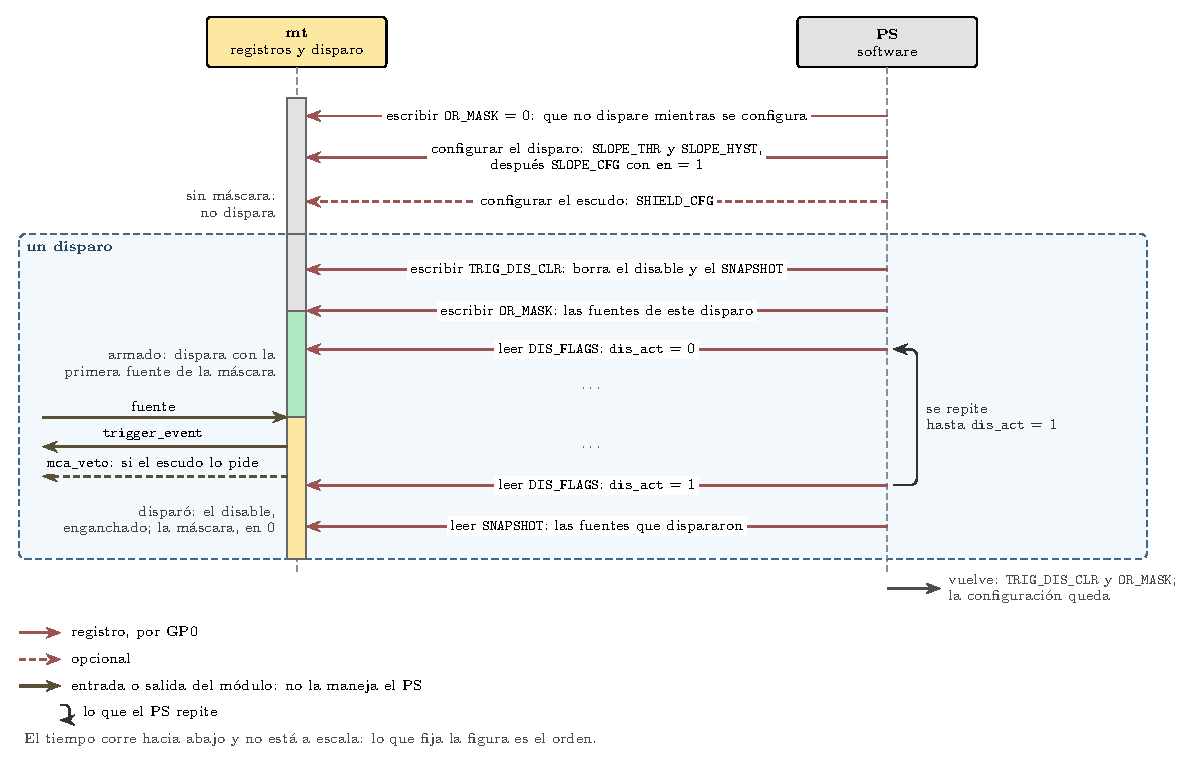
\includegraphics{cap3_mt_secuencia}
\caption[Secuencia de escrituras del PS y respuesta del multitrigger]{%
Secuencia de escrituras y lecturas del PS y respuesta del
multitrigger.\label{f:mt-secuencia}}
\end{figure}

%%%%%%%%%%%%%%%%%%%%%%%%%%%%%%%%%%%%%%%%%%%%%%%%%%%%%%%%%%%%%%%%%%%%%%%%%%%%%%%%
\section{Fuentes de \emph{triggering}}
\label{S:mt-fuentes}

La cantidad de \emph{triggers} disponibles en el módulo es parametrizable. El
diseño original contaba con $N_t=16$; como queríamos agregar fuentes con nuevos
tipos de eventos (nuestra primera idea fue agregar \emph{triggers} por pendiente), decidimos doblar la
cantidad a $N_t=32$. Podríamos tomar un número mayor, pero por un lado no lo
vimos necesario, porque no creemos que haga falta usar simultáneamente tantas
fuentes independientes, y por otro lado aumentar la cantidad requiere más
recursos y complejiza el \textbf{\emph{timing}}.

Los \emph{triggers} presentes en el diseño original consistían en los siguientes:
\begin{itemize}
  \item \textbf{ADC por nivel}: podemos decidir los que queramos, en un primer
    momento ponemos 4 dependiendo del modelo Red Pitaya (n/p).
  \item \textbf{ASG}: \emph{trigger} de la generación de señales interna (n/p).
  \item \textbf{\emph{External}}: \emph{triggers} externos (n/p).
  \item \textbf{Manual}: un \emph{trigger} manual.
\end{itemize}

%%%%%%%%%%%%%%%%%%%%%%%%%%%%%%%%%%%%%%%%%%%%%%%%%%%%%%%%%%%%%%%%%%%%%%%%%%%%%%%%
\section{Elección de fuentes}
\label{S:mt-eleccion}

Cada \emph{stream} de captura $i \in \{1,\ldots,N_\text{CH}\}$ decide el inicio de un
evento a partir de las mismas $N$ fuentes de disparo. Se instancia un
\codigo{mt\_trig\_src} por \emph{stream} de datos, y cada uno combina las fuentes en una única
señal de disparo. La pregunta de diseño es qué función de disparo
$f(\text{trig}_1,\ldots,\text{trig}_N)$ implementar.

En un primer momento parecería que la lógica combinacional es una buena idea.
Partimos de $f(\vec 0)=0$, es decir, si no tenemos ninguna fuente no queremos
un disparo de evento. Analizamos el caso más sencillo, dos entradas
($\text{trig}_1, \text{trig}_2$), para las que tenemos las siguientes
opciones:
\begin{itemize}
  \item OR($\text{trig}_1, \text{trig}_2$): independiente.
  \item AND($\text{trig}_1, \text{trig}_2$): coincidencia~\cite{Knoll2010,Rossi1930}.
  \item XOR($\text{trig}_1, \text{trig}_2$): anticoincidencia (veto)~\cite{Leo1994}.
\end{itemize}

La implementación combinacional tiene dos detalles:
\begin{enumerate}
  \item \textbf{Configuración exponencial.} Especificar $f$ arbitraria requiere
    su tabla de verdad, $2^N$ bits. El espacio de funciones con $f(\vec 0)=0$
    tiene $2^{2^N-1}$ elementos. Y aun para $N$ chico, obliga al usuario a
    enumerar todas las n-tuplas, lo que no es deseable.
  \item \textbf{Trabajo sobre el mismo ciclo de \emph{clock}.}
  \begin{enumerate}
    \item Una función combinacional compara las fuentes \textbf{en el mismo ciclo
      de reloj}. Distintos tipos de fuentes originarias de un mismo pulso
      (nivel, pendiente, externa) llegan con retardos relativos distintos y en
      general dependientes de la amplitud.
    \item Y en el caso de la entrada externa se suman la propagación y la
      sincronización entre dominios de reloj. Las latencias internas se pueden
      compensar en hardware, pero estas no. Una AND o una XOR de un solo ciclo
      es, entonces, frágil: su resultado depende del desfase entre fuentes y no
      sólo de qué fuentes se activaron.
  \end{enumerate}
\end{enumerate}

De las tres funciones vistas, la OR es la única que asegura la adquisición
independientemente del alineamiento de las fuentes en la entrada; esto quiere
decir que \textbf{al menos tenemos un \emph{trigger} por pulso} y como mucho
disparamos datos de más.
Para la AND y la XOR eso exige que los disparos coincidan exactamente, lo que en
la práctica no ocurre, y podemos obtener este análisis en un futuro mediante la
adquisición total y el procesamiento \emph{offline}.

%%%%%%%%%%%%%%%%%%%%%%%%%%%%%%%%%%%%%%%%%%%%%%%%%%%%%%%%%%%%%%%%%%%%%%%%%%%%%%%%
\section{Vulnerabilidades del mecanismo por OR}
\label{S:mt-vulnerabilidades}

El costo de la OR es que un \textbf{mismo pulso puede activar varias fuentes}, y una \textbf{OR sola lo
contaría como varios eventos}. Eso se resuelve con una
ventana de duración $W$ iniciada por el primer disparo. Durante esa ventana, los
disparos siguientes se consideran parte del mismo evento. En el diseño la
ventana se implementa en dos niveles:
\begin{itemize}
  \item El enganche \codigo{adc\_trg\_dis} de \codigo{mt\_trig\_src}, que
    bloquea el canal desde el ciclo siguiente al disparo;
  \item El \emph{holdoff} programable del \codigo{trigger\_shield}, que re-arma el
    canal (o veta a otros) recién al expirar.
\end{itemize}

%%%%%%%%%%%%%%%%%%%%%%%%%%%%%%%%%%%%%%%%%%%%%%%%%%%%%%%%%%%%%%%%%%%%%%%%%%%%%%%%
\section{Vista general del multitrigger}
\label{S:mt-vista-general}

En la Fig.~\ref{f:mt-panorama} se presenta el módulo. Sus bloques se agrupan por
función, que en la figura se distingue por color: la \textbf{detección} de las
fuentes, la \textbf{selección} de cuáles disparan, el \textbf{escudo} y los
\textbf{registros}. En la Tabla~\ref{t:mt-submodulos} se resume qué hace cada
submódulo.

\begin{figure}[H]
\centering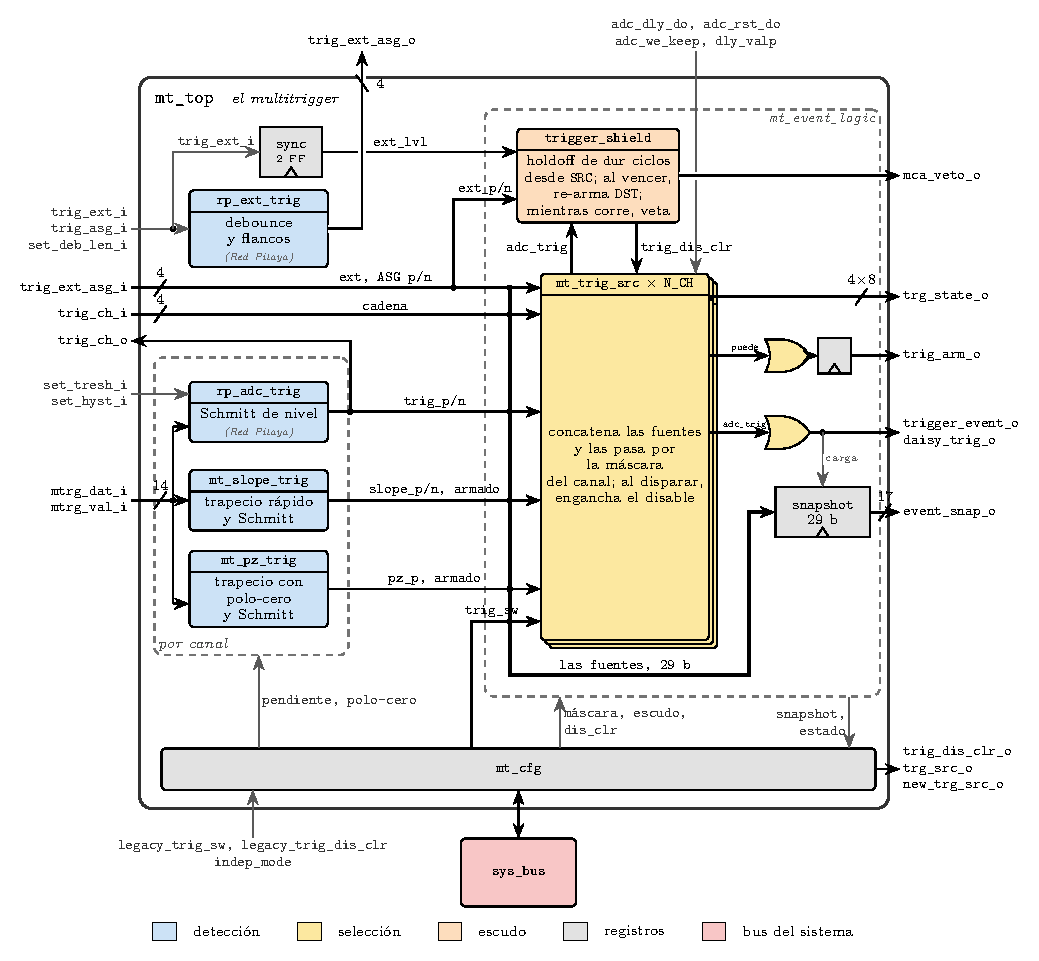
\includegraphics{cap3_panorama_mt}
\caption[Vista general del multitrigger]{%
Vista general del funcionamiento del módulo multitrigger.\label{f:mt-panorama}}
\end{figure}

\begin{table}[H]
\centering
\caption[Submódulos del multitrigger]{%
Submódulos del multitrigger.\label{t:mt-submodulos}}
\footnotesize
\setlength{\tabcolsep}{3pt}
\newcolumntype{Y}{>{\raggedright\arraybackslash}X}
\begin{tabularx}{\textwidth}{|>{\raggedright\arraybackslash}p{0.17\textwidth}|>{\raggedright\arraybackslash}p{0.18\textwidth}|Y|Y|}
\hline
\encabezado \textbf{Submódulo} & \textbf{Función} & \textbf{Entra / sale}
  & \textbf{Decisión de diseño} \\ \hline
\codigo{rp\_adc\_trig} & disparo por nivel, uno por canal
  & muestra $\rightarrow$ flancos \codigo{p}/\codigo{n}
  & el original de Red Pitaya~\cite{RedPitayaFPGA}, sin cambios \\ \hline
\codigo{rp\_ext\_trig} & entrada externa (DIO0\_P)
  & línea externa $\rightarrow$ flancos \codigo{p}/\codigo{n}
  & el original de Red Pitaya; el nivel se sincroniza aparte, para el veto
  \\ \hline
\codigo{mt\_slope\_trig} & disparo por pendiente, uno por canal
  & muestra $\rightarrow$ pulsos \codigo{p}/\codigo{n} y su re-armado
  & una derivada suavizada: el umbral no se mueve con la línea de base \\ \hline
\codigo{mt\_pz\_trig} & disparo por polo-cero, uno por canal
  & muestra $\rightarrow$ pulso y su re-armado
  & el trapecio del MCA, corto: no queda ciego en la cola de un pulso grande
  \\ \hline
\codigo{mt\_trig\_src} & selección de las fuentes de un canal
  & 29 fuentes $\rightarrow$ disparo del canal
  & máscara OR en lugar de un selector; enganche \codigo{adc\_trg\_dis} \\ \hline
\codigo{trigger\_shield} & escudo: \emph{holdoff} y veto
  & disparos y entrada externa $\rightarrow$ \emph{clear} por canal, veto al MCA
  & fuentes y destinos independientes, un solo contador \\ \hline
\codigo{mt\_event\_logic} & une los canales, el escudo y las salidas
  & disparos por canal $\rightarrow$ \codigo{trigger\_event},
    \codigo{trig\_arm}, \emph{snapshot}
  & no tiene lógica de disparo propia: es la topología \\ \hline
\codigo{mt\_cfg} & registros
  & bus del sistema $\rightarrow$ máscaras, escudo, umbrales
  & separado del bus del osciloscopio \\ \hline
\end{tabularx}
\end{table}

Las decisiones de diseño de los submódulos con lógica propia se presentan en la
Sec.~\ref{S:ap-mt-submodulos}. Los puertos y registros de todos están en sus
hojas de datos, en el repositorio.

\subsection{Función de \emph{timestamping}}
\label{S:mt-timestamping}

En el mismo ciclo de reloj del pulso de evento se captura el valor de un contador interno de la PL, que se mantiene hasta el
siguiente evento y funciona como referencia temporal. Este valor sale del módulo
y lo lee el OSC para hacer el \emph{timestamping} de los eventos medidos.

\subsection{Tiempo de relanzamiento}
\label{S:mt-relanzamiento}

Este se refiere al tiempo muerto propio del módulo~\cite{Knoll2010,Muller1973}.
Después de cada disparo, una fuente con histéresis~\cite{Schmitt1938} no puede
volver a disparar hasta re-armarse. Un pulso que llega en ese lapso no genera
flanco y el MCA no lo ve, así que no hay nada que contar. Lo único que se puede
medir es \textbf{cuánto tiempo estuvo desarmado el disparo}, y para eso el MT
expone el estado de re-armado de sus fuentes.

\subsubsection{Señal de re-armado de cada fuente}

Algunas fuentes exponen su señal de re-armado $a_i$, que vale 1 cuando la fuente
puede volver a disparar: los disparos por pendiente (\codigo{mt\_slope\_trig}) y
por polo-cero (\codigo{mt\_pz\_trig}). Las que no la tienen se consideran
siempre armadas, $a_i = 1$: las fuentes sin re-armado propio (manual, externa,
ASG y cadena) y el disparo por nivel (\codigo{rp\_adc\_trig}), que es el
original de Red Pitaya y no expone su estado.

\subsubsection{Relanzamiento del sistema con la OR}

Con la OR, el sistema dispara si dispara cualquiera de las fuentes habilitadas.
El criterio es entonces: \textbf{el sistema está en relanzamiento cuando ninguna
fuente habilitada puede disparar}, es decir, cuando todas están desarmadas. La
señal \codigo{trig\_arm} vale 1 fuera de ese estado. El criterio sólo usa las
señales de re-armado: quien lo consume no necesita saber qué disparo se utiliza.

\subsubsection{Cuándo mide los pulsos perdidos}

El tiempo de relanzamiento se mide para estimar cuántos pulsos se pierden. Ese
paso supone que, si alguna fuente está armada, el pulso se detecta, y eso sólo
vale si la fuente armada \textbf{reacciona a ese pulso}. La condición es
entonces que \textbf{cada fuente habilitada reaccione a todos los pulsos que se
miden}. Si se cumple, el tiempo de relanzamiento coincide con el tiempo en que
el disparo pierde pulsos: es la intersección de los intervalos desarmados de las
fuentes, ya que un pulso que llega con una fuente desarmada entra por otra que
esté armada.

Si no se cumple, una fuente puede estar armada sin reaccionar al pulso. Por
ejemplo, con el polo-cero de IN1 y el de IN2 habilitados y el MCA midiendo IN1:
después de un pulso en IN1, el polo-cero de IN1 queda desarmado, pero el de IN2
sigue armado porque no le llegó nada. \codigo{trig\_arm} vale 1, y un pulso que
llegue a IN1 en ese lapso se pierde contado como \emph{livetime}. Lo mismo pasa con dos
fuentes sobre la misma señal y umbrales distintos: con la de umbral bajo
desarmada, un pulso que no alcanza el umbral alto se pierde. En esos casos
$\mathtt{t\_rearm}$ es una cota inferior. También lo es con las fuentes que no
exponen su estado (nivel, externa), que cuentan como siempre armadas.

% Bibliografía de este capítulo. Va al final del archivo, siempre.
\bibliografiacapitulo

%%% Local Variables:
%%% mode: latex
%%% TeX-master: "template"
%%% End:
      % Implementación del multitrigger
% Origen: Secciones/PI - Implementacion MCA.md
% El "Apéndice" de la nota va en apend7.tex (Detalles del MCA). Lo que en la nota
% está entre %% (datapath del trapecio, funcionamiento interno del conformado,
% criterio de separación, elección de parámetros) no se transcribe.
\chapter{Implementación del MCA}
\label{C:implmca}

% Figuras de ESTE capítulo + las compartidas. Siempre al principio del archivo.
\graphicspath{{figs/cap7/}{figs/comunes/}}

\begin{destacado}
En este capítulo describimos (1) las funcionalidades ofrecidas por el módulo
MCA, (2) su método de utilización desde el PS, (3) una vista general del módulo
a nivel de HW, (4) el análisis del tiempo muerto y de los eventos perdidos, (5)
los métodos de recuperación del pulso y (6) los detalles de implementación de
cada submódulo. En el apéndice se presentan la detección del solape, la primera
versión del módulo, la elección de la cantidad de canales y el mapa de
registros. En el Cap.~\ref{C:resultados} se presentan las figuras de mérito
medidas para este módulo.
\end{destacado}

Este módulo tiene como entrada el flujo de muestras de los dos canales de
adquisición, ya calibradas y filtradas por el osciloscopio, y tres señales del
multitrigger (MT): el disparo \codigo{trig\_i}, que marca el comienzo de cada
evento, el veto \codigo{veto\_i} y el estado de re-armado del disparo,
\codigo{trig\_arm\_i}. Provee las siguientes funcionalidades:
\begin{itemize}
  \item \textbf{Histogramas de \emph{features} 1D y 2D}: un espectro de 8192 canales y
    un mapa de $128 \times 64$ bines. La cantidad de bines se fija en la
    síntesis; por registro se elige qué \emph{feature} va a cada eje y qué rango de
    ella cubre (\emph{zoom}).
  \item \textbf{Once \emph{features} por evento}, calculadas a la vez sobre el mismo
    pulso: pico, integral, dos de forma, la altura del conformado trapezoidal,
    y los tiempos y las marcas de solape con los pulsos vecinos
    (Tabla~\ref{t:implmca-estimadores}).
  \item \textbf{Medición de hasta \codigo{N\_ACC} eventos simultáneos}, cada uno
    en su ranura. El \emph{bitstream} trae \codigo{N\_ACC = 3}, y el registro
    \codigo{cfg\_n\_acc} elige cuántas se usan.
  \item \textbf{Banco de conformados trapezoidales} con corrección polo-cero:
    cada evento se publica con la forma más larga que sus vecinos permiten.
  \item \textbf{Línea de base} fija o con seguidor IIR.
  \item \textbf{Rechazo por criterios configurables}: una ventana de amplitud
    (sobre el pico o la integral) al cerrar cada evento, y un discriminador que
    acepta los eventos con una \emph{feature} elegida dentro, o fuera, de un
    intervalo.
  \item \textbf{Reporte del tiempo muerto y de los eventos perdidos}: el tiempo
    de adquisición desglosado por causa, la ocupación de las ranuras, tres
    estadísticos de los períodos muertos y un contador en cada punto donde se
    pierde o se rechaza un evento.
\end{itemize}

El criterio de finalización de eventos no se elige: la ventana la abre siempre
el disparo del MT y la cierra una compuerta fija. El cierre por histéresis se
retiró al pasar a medir varios pulsos a la vez, porque con ventanas superpuestas el
cruce de bajada es el de la señal sumada y cerraría todas juntas.

%==============================================================================
\section{Flujo de utilización del módulo}
\label{S:implmca-flujo}

En la Fig.~\ref{f:implmca-secuencia} se presenta el flujo de utilización.
Empieza con una \textbf{fase de configuración}, con \codigo{run = 0}, que se
realiza mediante el bus \emph{custom} de Pitaya. A continuación se usan los comandos de
control de la adquisición; en la figura se presenta la secuencia limpieza,
arranque, parada y lectura. Después de la limpieza (\codigo{CTRL.clear})
esperamos \codigo{clear\_busy = 0}, que indica que terminó el barrido de borrado
de los histogramas, y recién entonces arrancamos. Para leer, paramos con
\codigo{CTRL.run = 0} y esperamos \codigo{busy = 0}. Sin esa espera los valores
leídos no son estables: \codigo{run = 0} impide abrir ventanas nuevas, pero las
que estaban abiertas terminan de medir y el publicador sigue actualizando las
cuentas del histograma.

\begin{figure}[H]
\centering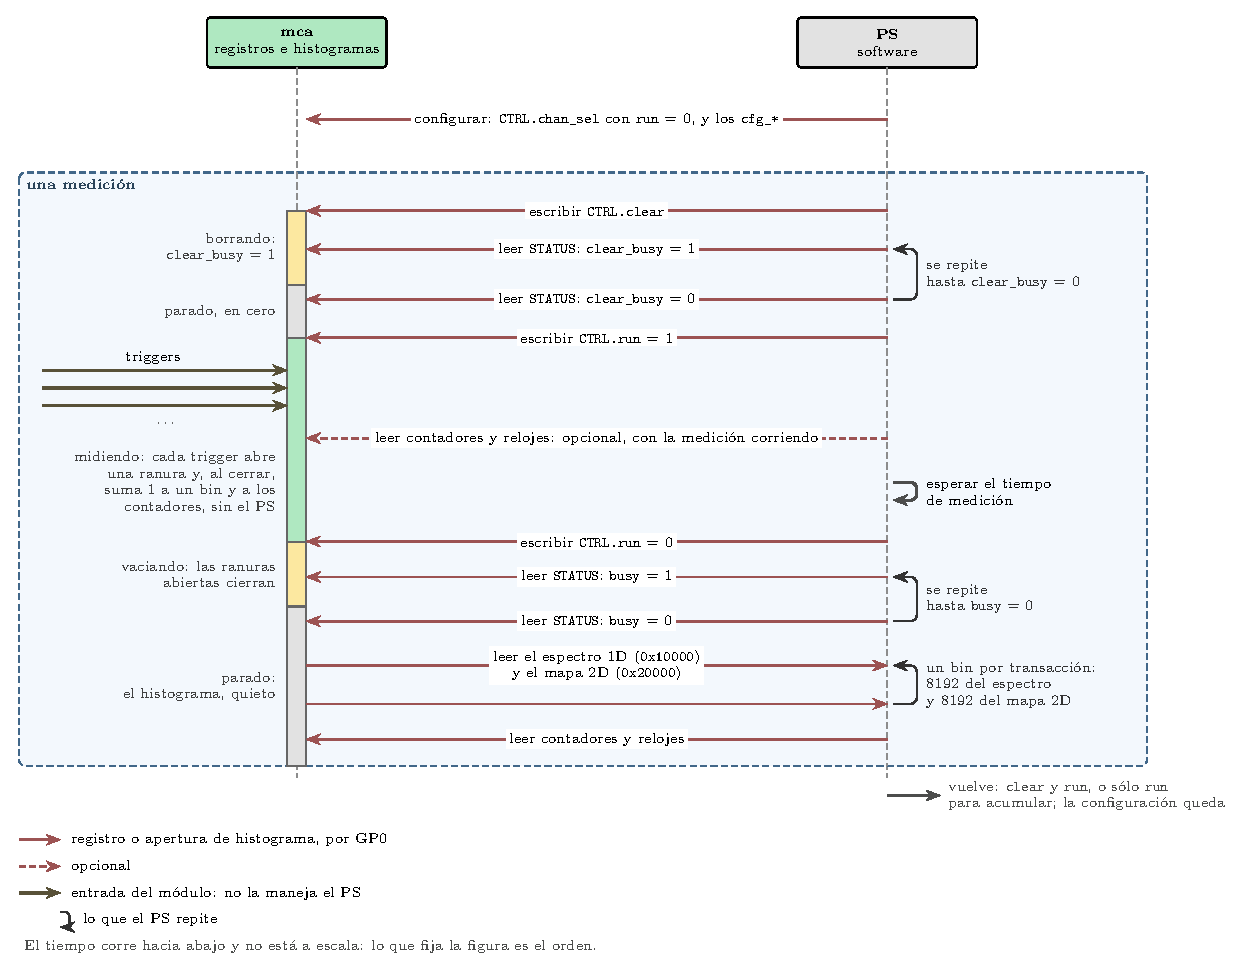
\includegraphics{cap7_secuencia_mca}
\caption[Flujo de utilización del MCA]{%
Flujo de utilización del MCA. Consiste en una fase de configuración y el
lanzamiento de medición.\label{f:implmca-secuencia}}
\end{figure}

Cuando un bin llega al tope ($2^{32}-1$) se levanta la bandera \codigo{full} de
ese histograma (\codigo{full\_1d} o \codigo{full\_2d}), que se mantiene hasta
la próxima limpieza. Por defecto el histograma entero deja de contar, y los
eventos que no entran van a \codigo{cnt\_full\_supp}. Así no hay \emph{overflow} en el
bin, y el espectro no se distorsiona: todos los canales dejan de contar en el
mismo instante, así que sus áreas relativas siguen siendo comparables. Los
relojes, en cambio, siguen corriendo, y la exposición del espectro congelado es
la del instante en que se levantó \codigo{full}. Con
\codigo{cfg\_keep\_full = 1} sólo ese bin queda en el tope y el resto sigue
contando.

%==============================================================================
\section{Vista general del módulo}
\label{S:implmca-vista-general}

En la Fig.~\ref{f:implmca-panorama} se presenta el módulo. La muestra llega con
el canal ya elegido, decimada y retrasada; el retardo compensa la latencia del
disparo del MT, de modo que la ventana abra en el pie del pulso. Los bloques se
agrupan por función, que en la figura se distingue por color. Todo corre en el
reloj del ADC (\qty{125}{\mega\hertz}) y procesa una muestra por ciclo.
\begin{enumerate}
  \item \textbf{Línea de base y conformado} (azul). Actúan sobre toda la señal,
    sin saber dónde hay pulsos: la línea de base \codigo{mca\_baseline}, fija o
    con un seguidor IIR, y el banco de trapecios \codigo{mca\_trap}, tres
    conformados trapezoidales de largos distintos. Se describen en la
    Sec.~\ref{S:implmca-recuperacion}.
  \item \textbf{Segmentación} (amarillo), en \codigo{mca\_window}:
  \begin{enumerate}
    \item Apertura: el flanco de \codigo{trig\_i}. El MCA no detecta pulsos por
      su cuenta: el disparo, y su re-armado, son del MT.
    \item Asignación: el asignador abre la ranura libre de menor índice. Si no
      hay ninguna libre, o si el veto está activo, el disparo se pierde y se
      cuenta (Sec.~\ref{S:implmca-perdidos}).
    \item Cierre: una compuerta fija de \codigo{gate\_long} muestras desde el
      disparo. Cada ranura retiene las compuertas al abrir y cierra sola.
  \end{enumerate}
  \item \textbf{Estadísticos} (verde):
  \begin{enumerate}
    \item Ranuras \codigo{mca\_slot} (\codigo{N\_ACC = 3}): cada una es un juego
      entero de acumuladores. Mientras su ventana está abierta actualizan
      versiones secuenciales de los estimadores: el pico y su instante, las
      cargas $Q_{tot}$ y $Q_{cola}$ y la suma de la meseta de cada forma del
      banco. Al abrir guardan las marcas de solape con otros disparos. Al cerrar
      aplican la ventana de amplitud: si el evento cae afuera, la ranura se
      libera sin publicar.
    \item Divisores \codigo{mca\_div\_restore} (dos, en paralelo): calculan las
      dos \emph{features} de forma, $Q_{cola}/Q_{tot}$ y $\text{pico}/Q_{tot}$, como
      fracciones de 16 bits.
  \end{enumerate}
  \item \textbf{Publicación} (naranja):
  \begin{enumerate}
    \item Publicador \codigo{mca\_publish}: atiende las ranuras cerradas de a
      una, en orden de cierre. Carga los divisores, elige la forma del banco,
      arma el \textbf{bus de \emph{features}} y libera la ranura: 18 ciclos por evento.
      Las ranuras cerradas son la cola de publicación; no hay una FIFO aparte.
    \item Selección de eje y \emph{zoom} \codigo{mca\_zoom}: un mux 16:1 por eje elige
      la \emph{feature}, y el \emph{zoom} la convierte en el índice del bin.
    \item Discriminador \codigo{mca\_discriminator}: acepta o rechaza el evento
      según una \emph{feature} cualquiera del bus.
    \item Histogramas \codigo{mca\_hist} (dos): el espectro 1D y el mapa 2D,
      cada uno en su BRAM, con un incremento por ciclo.
  \end{enumerate}
\end{enumerate}

En gris quedan el banco de registros y la contabilidad: los relojes de 64 bits,
la ocupación de las ranuras y los períodos muertos. Cada bloque se describe en
la Sec.~\ref{S:implmca-submodulos}.

\begin{figure}[H]
\centering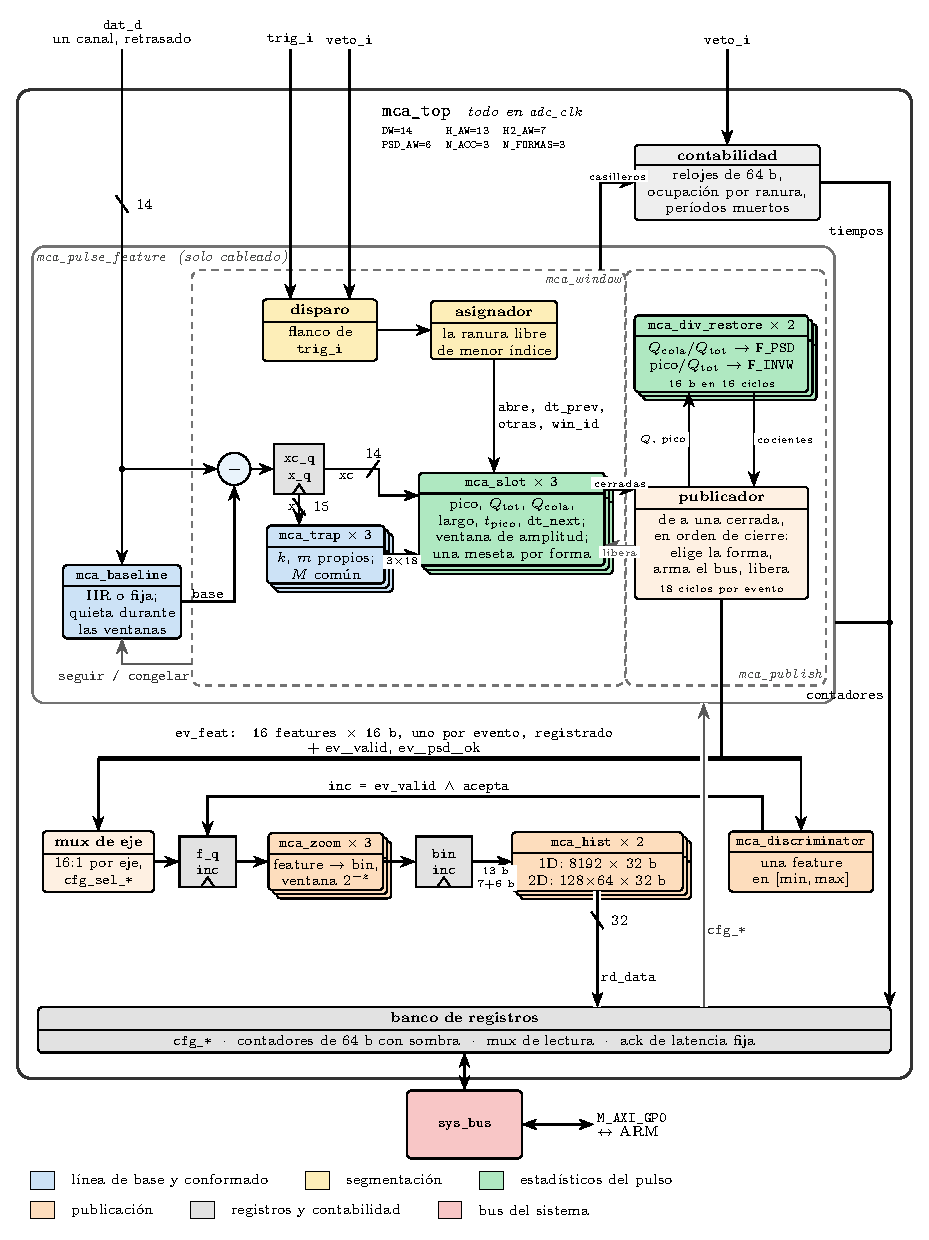
\includegraphics{cap7_panorama_mca}
\caption[Vista general del módulo analizador multicanal]{%
Vista general del módulo analizador multicanal. La muestra entra con el canal
ya elegido, decimada y retrasada, atraviesa \codigo{mca\_pulse\_feature} (la
línea de base, la ventana de medición y la publicación) y cae en el bus de
\emph{features}, del que cuelgan los ejes, el discriminador y los histogramas. El color
indica la función de cada bloque, y los números sobre las flechas son anchos en
bits.\label{f:implmca-panorama}}
\end{figure}

%==============================================================================
\section{Análisis de eventos perdidos}
\label{S:implmca-perdidos}

Seguimos el criterio de la Sec.~\ref{S:osc-tiempo-muerto}: recorremos el
\emph{datapath} y vemos qué hace cada etapa cuando no puede tomar un dato nuevo. Una
etapa \textbf{bloquea} si puede frenar a la anterior, y \textbf{descarta} si su
entrada no tiene \emph{ready} y el dato se pierde. Cada descarte tiene su
contador. En la Fig.~\ref{f:implmca-descarte} se presenta el \emph{datapath} del MCA
desde este punto de vista.

La primera etapa es el disparo, que es externo al MCA: lo genera el MT, y le
corresponde un tiempo de re-armado (Sec.~\ref{S:mt-relanzamiento}). Un pulso que
llega con el disparo desarmado no genera flanco y el MCA no lo ve, así que no
hay cuenta posible: lo que se mide es el tiempo desarmado. Después vienen tres
etapas que descartan y dos que sólo bloquean:
\begin{itemize}
  \item El \textbf{asignador} no puede frenar al disparo. Un disparo que llega
    bajo veto, o sin ranura libre, se pierde.
  \item Las \textbf{ranuras} y el \textbf{publicador} sólo bloquean. Mientras el
    publicador trabaja no libera la ranura que atiende, y las cerradas esperan;
    cuando no queda ninguna libre, el asignador no tiene dónde abrir. Esta
    contrapresión es la que se convierte en tiempo muerto.
  \item Los \textbf{histogramas} no pueden frenar al bus de \emph{features}. Un
    incremento que choca con una lectura del bus o con el barrido de borrado, o
    que llega con el histograma lleno, se pierde.
\end{itemize}

\begin{figure}[H]
\centering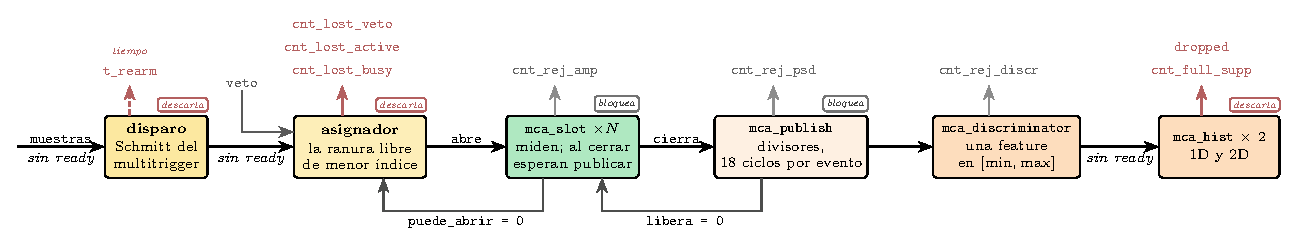
\includegraphics{cap7_freno_descarte}
\caption[\emph{Datapath} del MCA: dónde se frena y dónde se descarta]{%
Entrada por el módulo de multitrigger, \emph{datapath} principal del MCA y los
contadores asociados a cada fase. Las flechas rojas salen de las etapas que
descartan, cada una hacia su contador, y las de vuelta son la contrapresión de
las ranuras y del publicador, que sólo bloquean. Las grises son cortes por
criterio (amplitud, forma y discriminador), que no son tiempo
muerto.\label{f:implmca-descarte}}
\end{figure}

De la Fig.~\ref{f:implmca-descarte} salen dos medidas distintas de lo que se
pierde, y conviene no mezclarlas:
\begin{itemize}
  \item El \textbf{tiempo muerto} es un tiempo: el ancho de las ventanas en que
    la entrada descarta todo lo que llega. Sólo existe a la entrada, porque el
    disparo no se puede frenar: la contrapresión de las etapas que bloquean se
    convierte en tiempo muerto recién ahí. Se mide con relojes, y es lo que
    corrige la exposición del espectro.
  \item Los \textbf{descartes} son una cantidad: los eventos que se pierden en
    cualquier etapa de la cadena, cada uno en el punto en que ocurre. Se miden
    con contadores de eventos, uno por punto de descarte.
\end{itemize}

Las dos medidas sólo se cruzan en el asignador: cada disparo que se pierde ahí
es un descarte que cae dentro de una ventana de tiempo muerto, y por eso la
fracción perdida por el MCA se puede calcular de las dos maneras. En el resto de
la cadena son independientes. El tiempo muerto existe aunque en su ventana no
llegue ningún pulso, y los incrementos que pierde el histograma son descartes
sin tiempo muerto, porque el histograma no frena a nadie y la entrada sigue
abierta. Durante el re-armado del disparo pasa lo contrario: el pulso no genera
flanco, así que no hay descarte que contar y sólo se mide el tiempo. Los
descartes se miden con los contadores que se presentan a continuación, y el
tiempo muerto, con el teselado de la Sec.~\ref{S:implmca-teselado}.

En la Tabla~\ref{t:implmca-contadores} se presentan los contadores del módulo
que no son casilleros del teselado, y lo que representa cada uno. Son de cuatro
tipos: el \textbf{reloj} del barrido de borrado, que queda fuera del teselado;
los de \textbf{períodos}, que resumen los tramos sin ranura libre; los de
\textbf{arribos}, que cuentan disparos, y los de \textbf{incrementos}, que
cuentan eventos que no llegaron al histograma.

\begin{table}[H]
\centering
\caption[Contadores del tiempo muerto y de los eventos perdidos]{%
Contadores del tiempo muerto y de los eventos perdidos, además de los casilleros
del teselado (Tabla~\ref{t:implmca-teselado}) y de la ocupación de las ranuras
(Sec.~\ref{S:ap-mca-ocupacion}). \codigo{t\_clear} y \codigo{max\_dead\_len}
cuentan ciclos de \codigo{adc\_clk}; los demás, eventos. \codigo{cnt\_lost\_busy}
y los \codigo{dropped} de los dos histogramas se leen sumados en un solo
registro, y \codigo{cnt\_lost\_busy} se despeja del balance de
arribos.\label{t:implmca-contadores}}
\small
\begin{tabularx}{\textwidth}{|l|l|>{\raggedright\arraybackslash}X|}
\hline \encabezado \textbf{Tipo} & \textbf{Contador} & \textbf{Qué representa}
  \\ \hline
reloj & \codigo{t\_clear} & los ciclos del barrido de borrado \\ \hline
períodos & \codigo{cnt\_dead\_periods} & los tramos contiguos de ciclos sin
  ranura libre \\
 & \codigo{max\_dead\_len} & el largo del tramo más largo \\
 & \codigo{cnt\_dead\_ext} & los tramos con al menos un disparo adentro
  \\ \hline
arribos & \codigo{cnt\_cross} & los disparos con la adquisición en marcha:
  todos los arribos \\
 & \codigo{cnt\_open} & los disparos que abrieron una ranura \\
 & \codigo{cnt\_lost\_veto} & los disparos perdidos por el veto \\
 & \codigo{cnt\_lost\_active} & los disparos perdidos sin ranura libre, con
  todas midiendo \\
 & \codigo{cnt\_lost\_busy} & los disparos perdidos sin ranura libre, con
  alguna esperando al publicador \\ \hline
incrementos & \codigo{dropped} & los que chocaron con una lectura del bus o con
  el barrido de borrado \\
 & \codigo{cnt\_full\_supp} & los que llegaron con el histograma lleno y
  \codigo{cfg\_keep\_full = 0} \\ \hline
\end{tabularx}
\end{table}

El nombre \codigo{cnt\_cross} viene del MCA1, en el que el arribo era el cruce
del umbral del Schmitt propio (Sec.~\ref{S:ap-mca-mca1}); ahora cuenta
disparos, y el nombre se mantuvo para no cambiar el mapa de registros.

Además de los descartes hay \textbf{rechazos por criterio}: el evento se midió,
pero no cumple una condición configurada (la ventana de amplitud,
\codigo{cnt\_rej\_amp}; una forma inválida, \codigo{cnt\_rej\_psd}; el
discriminador, \codigo{cnt\_rej\_discr}). No son tiempo muerto, y no entran en
la tabla.

Con estos contadores planteamos dos balances. Valen ciclo a ciclo en el
hardware, pero cada lectura del bus tarda unos ciclos y los contadores avanzan
entre una y otra, así que se comprueban con la adquisición parada.
\begin{itemize}
  \item \textbf{Arribos.} Cada disparo con \codigo{run} suma a
    \codigo{cnt\_cross} y a exactamente uno de los contadores de pérdida o a
    \codigo{cnt\_open}, con la misma prioridad que el teselado
    (Sec.~\ref{S:implmca-teselado}): primero el veto y después la causa del
    bloqueo.
    \begin{equation}
      \mathtt{cnt\_cross} = \mathtt{cnt\_open} + \mathtt{cnt\_lost\_veto} +
      \mathtt{cnt\_lost\_active} + \mathtt{cnt\_lost\_busy}
      \label{e:implmca-balance-arribos}
    \end{equation}
  \item \textbf{Eventos.} Con las ranuras vacías (\codigo{busy = 0}), cada
    ventana abierta se cerró y, al cerrar, se publicó o se rechazó por
    amplitud, $\mathtt{cnt\_open} = \mathtt{cnt\_accepted} +
    \mathtt{cnt\_rej\_amp}$. De lo publicado, el espectro 1D cuenta todo salvo
    lo que rechaza el discriminador y lo que ese histograma descarta
    (\codigo{dropped}, \codigo{cnt\_full\_supp}); el 2D descarta además las
    formas inválidas.
\end{itemize}

%==============================================================================
\section{Teselado del tiempo de adquisición}
\label{S:implmca-teselado}

El tiempo muerto es el tiempo en que el sistema no puede procesar un evento
nuevo, y el tiempo vivo es su complemento (Sec.~\ref{S:mca-tiempo-muerto}). En
el MCA, un ciclo es \textbf{vivo} si un pulso que llegara en él abriría una
ranura, y \textbf{muerto} si se perdería. El tiempo vivo, $T_{live}$, es la
exposición del espectro: el tiempo durante el que el módulo pudo registrar
pulsos. Preferimos medirlo, junto con los tiempos muertos, antes que deducirlo
de un modelo. Un modelo supone cómo llegan los pulsos y cuánto dura cada período
muerto, y cualquier diferencia entre esa suposición y la fuente real se vuelve
un error de la corrección, que además crece con la tasa
(Sec.~\ref{S:mca-modelos-tiempo-muerto}).

La dificultad es que un pulso se puede perder por más de una causa, y las causas
se superponen. Se pierde si el veto del escudo del MT está activo, si no hay
ranura libre o si el disparo del MT todavía no se re-armó
(Sec.~\ref{S:mt-relanzamiento}). El veto puede llegar con todas las ranuras
midiendo, y el disparo puede estar desarmado mientras las ranuras están
ocupadas. Si cada causa tuviera su propio contador, un ciclo con dos causas
sumaría en los dos: la suma de los tiempos muertos superaría a
$T_{real} - T_{live}$, y no habría forma de repartir la pérdida entre los
bloques.

Por eso el tiempo de adquisición se \textbf{tesela}: se parte en casilleros que
no se superponen y que entre todos lo cubren, y cada ciclo con \codigo{run} suma
en exactamente uno. Cada casillero es un reloj de 64 bits, y cuando en un ciclo
se cumplen varias condiciones decide una prioridad fija, la del orden de la
Tabla~\ref{t:implmca-teselado}. Así ningún ciclo se cuenta dos veces ni queda
sin contar, el tiempo vivo y el muerto son complementarios por construcción, y
su suma es el tiempo real:
\begin{equation}
  T_{real} = T_{veto} + \underbrace{\mathtt{t\_win} +
  \mathtt{t\_div}}_{\text{muerto del MCA}} +
  \underbrace{\mathtt{t\_rearm}}_{\text{muerto del disparo}} + T_{live}
  \label{e:implmca-teselado}
\end{equation}

\begin{table}[H]
\centering
\caption[Casilleros del teselado del tiempo de adquisición]{%
Casilleros del teselado, en orden de prioridad: cada ciclo con \codigo{run}
suma en el primero cuya condición se cumple. Cuentan ciclos de
\codigo{adc\_clk}; \codigo{realtime}, $T_{real}$, cuenta todos los ciclos con
\codigo{run} y es su suma.\label{t:implmca-teselado}}
\small
\begin{tabularx}{\textwidth}{|l|>{\raggedright\arraybackslash}X|l|}
\hline \encabezado \textbf{Casillero} & \textbf{Suma cuando} &
  \textbf{Tiempo} \\ \hline
\codigo{vetotime} $T_{veto}$ & el veto está activo & excluido \\ \hline
\codigo{t\_win} & no hay ranura libre y todas están midiendo & muerto del MCA
  \\ \hline
\codigo{t\_div} & no hay ranura libre y alguna, ya cerrada, espera al
  publicador & muerto del MCA \\ \hline
\codigo{t\_rearm} & hay alguna ranura libre, pero el disparo del MT no se
  re-armó & muerto del disparo \\ \hline
\codigo{livetime} $T_{live}$ & hay alguna ranura libre y el disparo está
  armado & vivo \\ \hline
\end{tabularx}
\end{table}

La prioridad resuelve las dos superposiciones, y en los dos casos el orden tiene
un motivo:
\begin{itemize}
  \item \textbf{El veto va primero.} Es la convención de la compuerta de un
    MCA: mientras está cerrada, el reloj vivo se para, sea cual sea el estado
    interno. La cola de una ventana que termina bajo veto cuenta como tiempo
    vetado, y no como muerto.
  \item \textbf{El re-armado va después del tiempo muerto del MCA.} Sin ranura
    libre el pulso se pierde igual, esté o no armado el disparo, y si ese ciclo
    sumara también a \codigo{t\_rearm} la pérdida se contaría dos veces.
    \codigo{t\_rearm} es entonces el tiempo muerto que \textbf{agrega} el
    disparo cuando el MCA podía abrir, y \codigo{livetime} queda como lo que un
    pulso ve de verdad: una ranura libre y el disparo armado.
\end{itemize}
\codigo{t\_win} y \codigo{t\_div} no necesitan prioridad entre sí, porque los
distingue si alguna ranura espera al publicador.

\textbf{Por qué se subdivide el tiempo.} Para normalizar el espectro alcanzaría
con dos casilleros, vivo y muerto. Pero cada condición se calcula de forma
independiente, en una etapa distinta de la cadena: el veto en el escudo del MT,
el re-armado en el disparo y la falta de ranura libre en las ranuras del MCA.
Cada casillero representa así un descarte distinto del sistema, y guardarlo es
barato, porque es un contador más. Lo que hay que hacer para achicar cada uno
también es distinto:
\begin{itemize}
  \item \codigo{vetotime} no es tiempo muerto: es tiempo que se excluye a
    propósito, con el escudo del MT, y se descuenta de la exposición y de la
    tasa.
  \item \codigo{t\_rearm} es tiempo muerto del disparo, no del MCA. Se descuenta
    para estimar la tasa, porque en ese lapso ningún pulso genera disparo, y en
    la integración se le atribuye al MT
    (Sec.~\refpend{S:top-tiempo-muerto}{Implementación TOP: «Tiempo muerto por
    módulo», sección que ya no existe en la nota}).
  \item \codigo{t\_win} y \codigo{t\_div} son el tiempo muerto del MCA, pero por
    causas distintas. En \codigo{t\_win} todas las ranuras están midiendo, y
    sólo se achica con más ranuras o con una compuerta más corta. En
    \codigo{t\_div} hay ranuras cerradas que esperan al publicador, y se achica
    publicando más rápido. Con una sola ranura, \codigo{t\_div} es la
    publicación de cada evento; con varias debería ser casi nulo, y si no lo
    es, el cuello de botella es el publicador.
\end{itemize}

Con sólo el tiempo vivo y su complemento no se podría corregir la tasa, ni
saber qué bloque limita. De los casilleros salen los tres tiempos que se
reportan en cada adquisición: el vivo, $T_{live}$; el muerto del MCA,
$\mathtt{t\_win} + \mathtt{t\_div}$, y el del sistema, que le suma
$\mathtt{t\_rearm}$. Sus fracciones se toman sobre el tiempo no vetado,
$T_{real} - T_{veto}$, y con ellas se calculan la tasa de disparos y la fracción
perdida que se presentan al final de esta sección.

Fuera del teselado queda \codigo{t\_clear}, que cuenta los ciclos del barrido de
borrado. Durante el barrido las ranuras siguen midiendo, y lo que se pierde son
incrementos al histograma, que van a \codigo{dropped}: son descartes, y no
tiempo muerto.
\begin{itemize}
  \item \textbf{Tasa de disparos.} Durante el re-armado los pulsos no generan
    disparo, y los que llegan bajo veto se descuentan junto con su tiempo:
    \begin{equation}
      \hat\lambda = f_{clk}\,\frac{\mathtt{cnt\_cross} -
      \mathtt{cnt\_lost\_veto}}{T_{real} - T_{veto} - \mathtt{t\_rearm}}
      \label{e:implmca-lambda}
    \end{equation}
    Esta estimación supone que el disparo está armado mientras el MCA no tiene
    ranura libre. Por la prioridad del teselado, \codigo{t\_rearm} sólo cuenta
    con alguna ranura libre: el re-armado que queda detrás de las ranuras
    ocupadas no se descuenta, y si en ese lapso se pierden pulsos,
    $\hat\lambda$ los subestima.
  \item \textbf{Fracción perdida por el MCA.} Con arribos de Poisson, la
    fracción de pulsos que encuentran al módulo sin ranura libre es la fracción
    del tiempo en que no hay ninguna~\cite{Wolff1982}, y se puede calcular de
    las dos maneras:
    \begin{equation}
      P_{MCA} = \frac{\mathtt{t\_win} + \mathtt{t\_div}}{T_{real} - T_{veto}}
      \simeq \frac{\mathtt{cnt\_lost\_active} +
      \mathtt{cnt\_lost\_busy}}{\mathtt{cnt\_cross} - \mathtt{cnt\_lost\_veto}}
      \label{e:implmca-pmca}
    \end{equation}
    La primera mira el tiempo y la segunda los arribos contados. Con otro
    proceso de arribos, como el de un generador periódico, dejan de coincidir.
\end{itemize}

Los modelos de tiempo muerto, que predicen estos valores a partir de la tasa y
del largo de la ventana, se presentan en la Sec.~\ref{S:ap-mca-modelos}.

%==============================================================================
\section{Métodos de recuperación del pulso}
\label{S:implmca-recuperacion}

El punto de partida de todos los métodos es el disparo de eventos: cada disparo
marca dónde empieza un pulso, y el MCA lo mide en una ventana que arranca ahí.
Cuando dos pulsos se superponen, la ventana de uno contiene parte del otro, y hay
cuatro políticas posibles, que se presentan en la
Tabla~\ref{t:implmca-politicas}.

\begin{table}[H]
\centering
\caption[Políticas para un pulso que se superpone con otro]{%
Políticas para un pulso que se superpone con otro. Las tres primeras procesan cada
evento por separado, a medida que llegan las muestras; la cuarta tiene que
procesar juntos los eventos del par.\label{t:implmca-politicas}}
\small
\begin{tabularx}{\textwidth}{|>{\raggedright\arraybackslash}p{0.17\textwidth}%
  |>{\raggedright\arraybackslash}X|>{\raggedright\arraybackslash}X%
  |>{\raggedright\arraybackslash}X|>{\raggedright\arraybackslash}X|}
\hline \encabezado & \textbf{Sin corrección (1)} & \textbf{Descartar (2)} &
  \textbf{Rescate único (3)} & \textbf{Rescate total (4)} \\ \hline
Qué se hace con un pulso superpuesto & se mide igual, y sale contaminado & se mide
  y se marca, y no llega al histograma & se mide con un estimador que no ve a
  sus vecinos & se mide junto con sus vecinos, y se separan \\ \hline
Eventos publicados por disparo & 1 & 0 o 1 & 1 & 1 \\ \hline
Entrada al cálculo de \emph{features} & flujo de muestras & flujo de muestras & flujo
  de muestras & por transacción: los eventos del par, juntos \\ \hline
En este MCA & la primera versión, el MCA1 & las marcas de solape y el
  discriminador & el banco de trapecios, en \codigo{F\_TRAP} & no se
  implementó \\ \hline
\end{tabularx}
\end{table}

El MCA actual combina la (2) y la (3): todo disparo que encuentra una ranura
libre se mide, las marcas de solape dicen si el resultado está contaminado, y
\codigo{F\_TRAP} usa la forma del banco cuya ventana no alcanza a los vecinos. La
(4) es la descomposición de los estimadores del par: con la distancia entre los
dos pulsos, un sistema lineal de $2 \times 2$ separa sus amplitudes. Se
descartó porque es muy sensible a un error de una muestra en esa distancia, y
porque obliga a retener el primer evento hasta que cierre el segundo.

\subsection{Cálculo secuencial de estimadores}
\label{S:implmca-secuencial}

En los casos (1), (2) y (3) las muestras ingresan al MCA en forma de un flujo, y
simplemente tenemos que actualizar el valor del estadístico de la ventana con
cada muestra nueva, hasta que la ventana termina. Esto se implementa con una
señal de habilitación y simplifica extremadamente el flujo de datos de la
aplicación. El desarrollo matemático formal consiste en poder expresar
$f(x_{i,\ldots, n}) = g( f(x_{i,\ldots, n-1}), x_n)$: no es más que
\textbf{descomponer la aplicación sobre $n$ elementos en los primeros $n-1$ y el
último}; en particular, cuando $f=g$ la operación es asociativa. Ejemplo para la
suma $Q_n$ (integral discreta) y el máximo $A_n$:
\begin{equation}
\begin{aligned}
A_n&= \max_{i=0,\ldots, n} A(x_i) = \max \left( \max_{i=0,\ldots, n-1} A(x_i),
  A(x_n) \right) = \max ( A_{n-1} , A(x_n)) \\
Q_n&= \sum_{i=0,\ldots, n} A(x_i) = \left( \sum_{i=0,\ldots, n-1} A(x_i)
  \right) + A(x_n) = Q_{n-1} + A(x_n)
\end{aligned}
\label{e:implmca-secuencial}
\end{equation}
La aplicación de estas propiedades requiere dos cosas:
\begin{itemize}
  \item \textbf{Un registro por estimador y por ventana abierta}: es lo que
    tiene cada ranura.
  \item \textbf{Arbitrar la publicación}: las ventanas cierran en cualquier
    momento, pero hay un solo publicador, con sus dos divisores, y el histograma
    acepta un incremento por ciclo, porque su BRAM usa un puerto para leer el
    bin y el otro para escribirlo. Por eso las ranuras cerradas esperan su
    turno en una cola.
\end{itemize}

\subsection{Recuperación de la línea de base}
\label{S:implmca-linea-base}

El método más ingenuo de recuperación de la línea de base sería, dada una
ventana completa de un pulso, restarle su media $\bar A$. Esto daría un nuevo
vector de datos compensados, cuyos estadísticos resultan equivalentes a
calcular las siguientes correcciones: $A_{rec} = A - \bar A$, mientras que para
la carga $Q_{rec} = Q - N_{med} \bar A=0$. Igualmente, esto tiene varios
problemas:
\begin{enumerate}
  \item El pulso compensado queda con valor medio 0. Esto está mal, ya que
    muchas de las conformaciones son \textbf{unipolares}, y entonces esto daría
    una desviación sistemática negativa.
  \item No tiene en cuenta que lo que está debajo del pulso cambia a lo largo de
    la ventana. Ahí hay dos cosas distintas: la \textbf{línea de base continua},
    que deriva lentamente, y la \textbf{cola de los pulsos anteriores}, que
    sigue la forma del conformado. Restar una media no corrige ninguna de las
    dos en un estadístico puntual como la amplitud máxima: la primera necesita
    un seguimiento, y la segunda, conocer la forma del pulso.
\end{enumerate}

\subsubsection{Metodologías básicas de recuperación de la línea de base}
\label{S:implmca-lb-basicas}

Las metodologías básicas de recuperación de la línea de base son dos: una
compensación fija, con $b$ = \codigo{cfg\_baseline}, y un seguidor IIR, que
sigue la media de la señal:
\begin{equation}
  b[n] = b[n-1] + 2^{-k}\,\big(v[n] - b[n-1]\big)
  \label{e:implmca-iir}
\end{equation}
Es un pasabajos recursivo de un polo, la media móvil
exponencial~\citecap{Smith1997}{19}. El seguidor es especialmente útil si
tenemos un conformado RC. Se elige una u otra con \codigo{cfg\_bl\_auto}. El
seguidor se queda quieto mientras alguna ranura mide y durante
\codigo{cfg\_bl\_holdoff} muestras después de cada cierre: si siguiera apenas
cierra la compuerta, tomaría la cola y el \emph{undershoot} del pulso como base,
y la arrastraría hacia el lado equivocado.

Estas metodologías se utilizaron en las primeras versiones del sistema y no se
las quitó por dos razones: (1) por su bajo costo y (2) porque son procesamientos
tan generales que no están especializados en ciertas formas de pulsos, como las
que se presentan a continuación.

\subsubsection{Metodologías avanzadas de recuperación de la línea de base}
\label{S:implmca-lb-avanzadas}

Hasta la Sec.~\ref{S:implmca-lb-basicas} teníamos un procesamiento que (1) no tenía en cuenta
la señal de entrada y (2) era un filtro simple. Los métodos avanzados tienen en
cuenta la familia de los pulsos y los disparos. Hay dos familias:
\begin{itemize}
  \item \textbf{Corrección por modelo del pulso}: suponemos que la entrada es la
    superposición de varios pulsos, $f(t) = A(t) + B(t) + C(t) + \ldots$, y a lo
    largo del tiempo estimamos cada uno, $(\hat A(t), \hat B(t), \hat C(t),
    \ldots)$, para restarle a cada medida la cola de los anteriores. Con el
    disparo en $t_0$ hacemos la estimación inicial de $A$, y nuestro
    conocimiento del conformado da el resto del pulso. Necesita un estado por
    pulso, y su error crece con el error en la distancia entre los disparos.
  \item \textbf{Corrección por filtrado}: no se descompone la señal en pulsos.
    Un mismo filtro lineal se aplica a toda la señal, sin saber dónde hay
    pulsos, y convierte cada pulso en una forma de duración finita; dos pulsos
    se pueden medir por separado si esas formas no se pisan, y eso lo deciden
    los disparos. Uno de estos filtros es el conformado trapezoidal. No necesita
    toda la serie del pulso: su salida en cada muestra depende sólo de las
    últimas $2k+m$, y la medida, de unas $k+m$ desde el pie del pulso.
\end{itemize}

Las dos familias están emparentadas: la deconvolución que usa el trapecio,
$y[n] - a\,y[n-1]$, es la extrapolación de la cola con un predictor de una
muestra, aplicada a toda la señal. A continuación describimos la corrección por
filtrado, que es la que implementa el MCA.

\subsection{Utilización de trapecios en el multitrigger y en el MCA}
\label{S:implmca-rapido-lento}

Utilizamos la conformación trapezoidal en dos etapas; esta es la arquitectura
clásica de \textbf{canal rápido y canal lento} (\emph{fast} y \emph{slow
filter}): un filtro corto para saber cuándo y cuántos pulsos hay (el trabajo de
segmentación), y uno largo para determinar los estimadores. En el MCA es el
banco de formas que mide \codigo{F\_TRAP}. En el multitrigger es una fuente de
disparo, \codigo{mt\_pz\_trig}, de un ciclo, mientras que en el MCA se toma la
suma de la meseta en la ventana, \codigo{F\_TRAP}. Los dos usan la misma cuenta
y el mismo \codigo{Mq}.

\subsection{Recuperación por conformación}
\label{S:implmca-trapezoidal}

Esta sección es el análisis del \textbf{canal lento}
(Sec.~\ref{S:implmca-rapido-lento}): el filtro largo que mide la amplitud de
cada pulso, una vez que el canal rápido, el disparo del MT, dijo cuándo llegó y
a qué distancia están sus vecinos.

Si quisiéramos simplemente compensar la cola del conformado, podríamos utilizar
una deconvolución de Jordanov~\cite{Jordanov1994}, que requiere únicamente dos
muestras consecutivas del pulso:
\begin{equation}
  x_d[n] = y[n] - a\,y[n-1], \qquad a = e^{-1/\tau}
  \label{e:implmca-deconv}
\end{equation}
Si $y[n] = A\,e^{-n/\tau}$, el resultado es un impulso de área $A$: la cola
desaparece, y un segundo pulso montado sobre ella mide como si estuviera solo.
El problema es que no promedia el ruido. La amplitud se estima sumando $x_d$ en
unas pocas muestras desde el pie, y esa suma es, en esencia, una muestra después
del pie menos una antes: con ruido blanco $\sigma$ por muestra, su error es
$\approx \sqrt{2}\,\sigma$, sea cual sea el largo de la suma. Mide incluso peor
que el pico, que se compara contra una base promediada sobre miles de muestras.

El conformado trapezoidal de Jordanov y Knoll~\cite{Jordanov1994} resuelve eso
sin perder la compensación de la cola: es la misma deconvolución seguida de dos
sumas móviles, de $k$ y de $l = k+m$ muestras,
\begin{equation}
  H(z) = 16\,(1+M)\,\underbrace{\left(1 - a_M\,z^{-1}\right)}_{\text{deconvolución}}
  \,B_k(z)\,B_l(z), \qquad B_k(z) = \sum_{i=0}^{k-1} z^{-i}, \qquad
  a_M = \frac{M}{1+M}
  \label{e:implmca-trapecio}
\end{equation}
donde $M$ es la constante polo-cero, que se elige para que $a_M = a$
(Sec.~\refpend{S:ap-mca-conformado}{detalles de la conformación
trapezoidal: esa sección de la nota está comentada}). Si $M$ no coincide con la
cola del pulso, la cancelación no es exacta: a la salida queda un resto de la
cola, una exponencial de constante $\tau$ que sigue después del trapecio, y un
pulso que llega encima la suma a su altura. Cuánto pesa un error en $M$ se
presenta en la Sec.~\ref{S:res-polo-cero}. Es \textbf{lineal}, y con una entrada
exponencial $x = A\,e^{-n/\tau}$ la salida tiene tres regiones: una subida de
$k$ muestras, una meseta de $m$ y una bajada de $k$. Se presenta en la
Fig.~\ref{f:implmca-trapecio}. Su largo total es $2k+m$ por larga que sea la
cola de la entrada, y esa huella finita es lo que permite separar pulsos
apilados. La deconvolución sola es el caso $k = 1$, porque $B_1 = 1$: en el
hardware la pregunta no es deconvolución o trapecio, sino qué $k$. En la
Sec.~\refpend{S:ap-mca-conformado}{detalles de la conformación trapezoidal:
esa sección de la nota está comentada} se muestra cómo se obtiene analíticamente
y en HW.

\begin{figure}[H]
\centering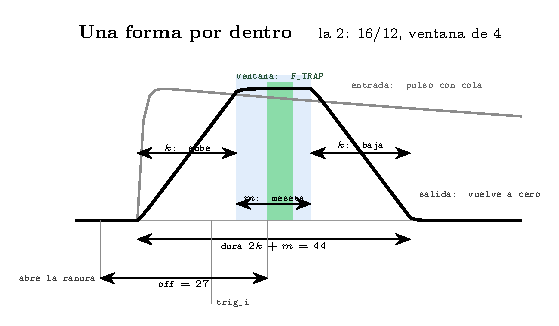
\includegraphics[width=0.6\linewidth]{cap7_trapecio_anatomia}
\caption[Forma básica del conformado trapezoidal]{%
Forma básica del conformado trapezoidal. Consta de una subida de $k$ muestras,
una meseta de $m$ y una bajada del mismo tiempo de subida
$k$.\label{f:implmca-trapecio}}
\end{figure}

La tolerancia al ruido de un conformado trapezoidal depende de $k$. En la
Fig.~\ref{f:implmca-deconv-error} se presentan, contra $k$, dos estadísticos
obtenidos por Monte Carlo: el error relativo de la amplitud de un pulso solo,
que es el ruido de la medición, y la separación mínima a la que el segundo pulso
de un par mide sin sesgo. El ruido baja como $\sigma\sqrt{2/k}$ y la separación
crece como $2k+m$: cuadruplicar $k$ divide el ruido por dos, y cada muestra que
se agrega a $k$ se agrega también a la separación. El punto $k = 1$ es la
deconvolución sola.

\begin{figure}[H]
\centering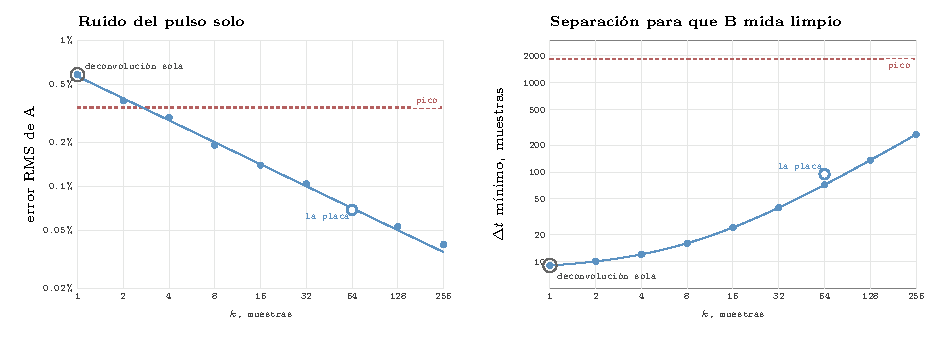
\includegraphics{cap7_trap_deconvolucion}
\caption[Ruido y separación mínima contra $k$]{%
Ruido de la amplitud de un pulso solo (izquierda) y separación mínima para que
el segundo pulso de un par mida sin sesgo (derecha), contra $k$. El punto
$k = 1$ es la deconvolución sola.\label{f:implmca-deconv-error}}
\end{figure}

Además del compromiso entre ruido y separación, el trapecio tiene las siguientes
propiedades:
\begin{itemize}
  \item \textbf{Promedia el ruido.} Pesa con $\approx +1/k$ las $k$ muestras
    después del pie y con $\approx -1/k$ las $k$ de antes: es la diferencia de
    dos promedios de $k$ muestras. Con ruido blanco, es el estimador lineal de
    mínima varianza para la altura de un escalón con ese largo, y su error es
    $\sigma\sqrt{2/k}$. Este efecto se representa en la
    Sec.~\ref{S:res-ruido}.
  \item \textbf{Saca la cola de los pulsos anteriores, pero no la línea de base
    continua.} El término polo-cero convierte cada exponencial en un escalón,
    así que la «base» que se mueve con el apilamiento desaparece de la cuenta.
    Una base continua, en cambio, pasa: un error de base $\varepsilon$ es un
    escalón constante en la entrada, y el trapecio lo deja pasar con ganancia
    $16\,k\,l$. Relativo a la altura de un pulso de amplitud $A$, que es
    $16\,A\,k\,(1+M)$, corre la medida en
    \begin{equation}
      \frac{\Delta A}{A} = \frac{\varepsilon}{A}\,\frac{l}{1+M} \approx
      \frac{\varepsilon}{A}\,\frac{l}{\tau}
      \label{e:implmca-error-base}
    \end{equation}
    Es menos que en el pico, porque $l < \tau$, pero no se cancela. Por eso la
    base se resta antes del trapecio (Sec.~\ref{S:implmca-lb-basicas}).
  \item \textbf{Tolera la pérdida balística y el \emph{jitter} del disparo.} La pérdida
    balística se presenta en la Sec.~\ref{S:mca-tipos-conformado}. El trapecio
    de un pulso real es el ideal convolucionado con su subida, de largo $t_c$:
    las esquinas se redondean y la parte plana de la meseta se achica a
    $\approx m - t_c$. Mientras $m$ supere $t_c$ más la variación del instante
    de disparo, y la ventana de promedio caiga en la parte plana, la altura no
    depende de la subida: no hay déficit balístico. Con $m \le t_c$ no queda
    meseta, y la altura depende de la forma del pulso sin aviso.
  \item \textbf{Es barato.} Dos acumuladores y una multiplicación (el término
    $M$), en enteros, para cualquier $k$ y $m$, más tres líneas de retardo en
    memoria. Uno solo sirve a todas las ranuras.
  \item \textbf{Junto con el canal rápido, dice cuándo midió limpio.} Como la
    huella dura $2k+m$ muestras, el segundo pulso de un par mide limpio si llega
    a más de $\approx k+m$ muestras del primero. Las distancias no las da el
    trapecio sino los disparos del MT, en \codigo{F\_DTPREV} y
    \codigo{F\_DTNEXT} (Sec.~\refpend{S:ap-mca-separacion}{criterio de
    separación: esa sección de la nota está comentada}).
\end{itemize}

\subsection{Utilización del banco de trapecios}
\label{S:implmca-banco}

Para el conformado trapezoidal tenemos un compromiso entre la capacidad de
discernir la separación de pulsos y la precisión de la determinación del
estadístico; este se presenta en la Fig.~\ref{f:implmca-banco-par}. Es
importante notar que no tenemos un conformado por ranura, sino que el
\textbf{tipo de conformado se aplica a toda la señal}. La utilización de un
banco de conformados consiste en aplicar diferentes largos ($k$ y $m$), con la
misma $M$.

\begin{figure}[H]
\centering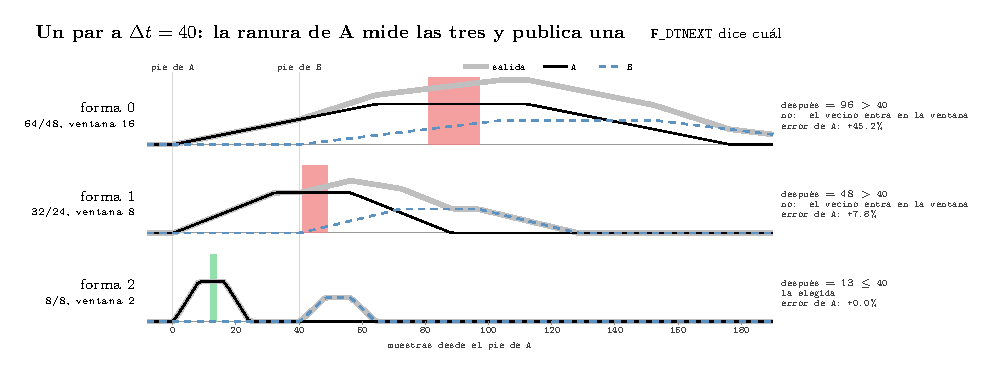
\includegraphics{cap7_banco_formas_par}
\caption[Trapecios de distintas formas sobre un par de pulsos superpuestos]{%
Aplicación de trapecios de forma 64/48, 32/24 y 8/8 para un mismo par de pulsos
superpuestos con $\Delta t=40$. Cada fila es la salida de una forma (gris) con
el aporte de cada pulso por separado, y la ventana en que la ranura de A
promedia la meseta. En las dos formas largas el pulso B entra en esa ventana
(rojo); la 8/8 es la única que queda limpia (verde), y es la que se publica,
porque \codigo{F\_DTNEXT} dice que el vecino está a 40
muestras.\label{f:implmca-banco-par}}
\end{figure}

Es así que, cuando tenemos un disparo, calculamos los elementos para
conformados de diferentes parámetros y, dados los disparos en la ventana,
descartamos los anchos con superposiciones identificadas. La estimación por el
trapecio resulta del \textbf{conformado válido de mayor longitud}. En la
Fig.~\ref{f:implmca-banco-uso} se presenta este mecanismo para conformados de
largo 64/48, 32/24 y 8/8. Para el primer pulso no tenemos ningún otro disparo en
las 97 muestras previas ni en las 96 posteriores al primer disparo P1, de forma
que se decide publicar el primer trapecio (remarcado en azul oscuro). Para el
segundo disparo, P2, hay un disparo durante la ventana posterior del banco
64/48, de forma que se elige el segundo como el mejor. El mismo criterio aplica
para el resto de los disparos.

\begin{figure}[H]
\centering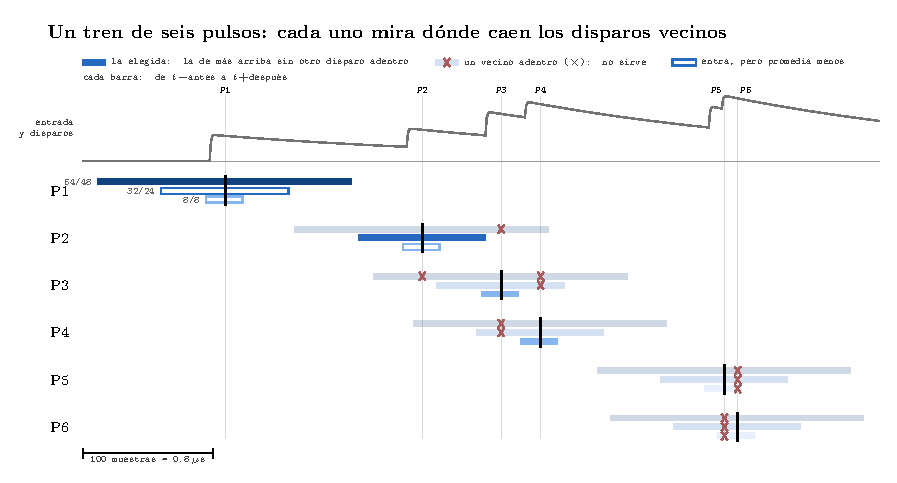
\includegraphics{cap7_banco_uso}
\caption[Esquema de utilización del banco de trapecios]{%
Esquema de utilización del banco de trapecios; cada uno representa un canal
lento de diferente largo. Presentamos los largos 64/48, 32/24 y
8/8.\label{f:implmca-banco-uso}}
\end{figure}

%==============================================================================
\section{Detalles de submódulos}
\label{S:implmca-submodulos}

En esta sección se presentan los detalles de implementación de los submódulos
de la Fig.~\ref{f:implmca-panorama}. Si se quiere ir al \emph{ground truth}, hay
que analizar el RTL de los módulos, en el directorio \ruta{prj/MCA/modulos/mca}
del repositorio del proyecto \incompleto{} (falta el enlace).
\codigo{mca\_pulse\_feature} sólo conecta \codigo{mca\_window} con
\codigo{mca\_publish}, y la línea de base y el banco de trapecios se presentan en
la Sec.~\ref{S:implmca-recuperacion}, así que no tienen subsección propia.

\subsection{Utilización de ranuras y elección de estimadores}
\label{S:implmca-estimadores}

Cada evento se publica con todos sus estimadores a la vez, en un \textbf{bus de
\emph{features}} de 16 posiciones de 16 bits (Fig.~\ref{f:implmca-bus}). El bus es
interno: el ARM no lo ve, y lo que configura es qué posición alimenta cada eje
del histograma y cuál mira el discriminador. Como las posiciones son fijas,
cambiar de estimador no cambia el \emph{bitstream} ni los pulsos medidos: el mismo
pulso puede ir al espectro por su pico y al mapa 2D por su integral y su forma.

Llamamos $x = v - b$ a la muestra $v$ con la línea de base $b$ restada, y
$x_c = \max(x, 0)$ a la misma \textbf{recortada a cero}. Numeramos las muestras
de la ventana desde el disparo, $n = 0$, hasta la compuerta larga $G_l$ =
\codigo{gate\_long}, y contamos sólo las muestras válidas. Las dos cargas son
\begin{equation}
  Q_{tot} = \sum_{n=0}^{G_l-1} x_c[n], \qquad Q_{cola} = \sum_{n=G_s}^{G_l-1}
  x_c[n]
  \label{e:implmca-cargas}
\end{equation}
con $G_s$ = \codigo{gate\_short}, la \textbf{compuerta corta}. $Q_{cola}$ es la
carga que llega después de $G_s$ muestras del disparo, y su fracción de
$Q_{tot}$ mide cuánto pesa la componente lenta del pulso: es el método de
comparación de carga~\cite{Brooks1959}, con el que se distinguen, por ejemplo,
los neutrones de los gammas en un centellador orgánico. Que $G_s$ se cuente
desde el disparo, y no desde el pico, hace a $Q_{cola}$ inmune al \emph{jitter} del
instante del pico. \codigo{F\_TRAP}, en cambio, no suma en toda la ventana sino
en una \textbf{región de la meseta} propia de cada forma del banco: $2^{lw}$
muestras que empiezan \codigo{off} muestras después del disparo, configuradas
por forma con \codigo{cfg\_trap\_off} y \codigo{cfg\_trap\_lw} (se detalla en la
Sec.~\ref{S:implmca-slot}). En la Tabla~\ref{t:implmca-estimadores} se presenta
el procesamiento que recibe cada estimador.

\begin{table}[H]
\centering
\caption[Estimadores del bus de \emph{features}]{%
Estimadores del bus de \emph{features}, agrupados por lo que miden, y el procesamiento
que recibe cada uno. Los tiempos y separaciones se cuentan en muestras válidas.
Los estimadores de solape no miran la señal sino los disparos del MT; cómo se
calculan se detalla en la Sec.~\ref{S:ap-mca-solape}. Las posiciones 11 a 15
del bus están reservadas.\label{t:implmca-estimadores}}
\footnotesize
\begin{tabularx}{\textwidth}{|l|l|>{\raggedright\arraybackslash}p{0.3\textwidth}%
  |>{\raggedright\arraybackslash}X|}
\hline \encabezado \textbf{Tipo} & \textbf{Estimador} & \textbf{Qué representa}
  & \textbf{Procesamiento} \\ \hline
amplitud & \codigo{F\_PEAK} & la altura del pulso en su muestra más alta &
  resta de la línea de base, recorte a cero y máximo de las muestras de la
  ventana \\
 & \codigo{F\_INT} & la carga del pulso, $Q_{tot}$ & resta de la línea de base,
  recorte a cero y suma de todas las muestras de la ventana, corrida
  \codigo{cfg\_q\_shift} bits \\
 & \codigo{F\_TRAP} & la altura del pulso, promediada sobre la meseta del
  trapecio~\cite{Jordanov1994} & resta de la línea de base, conformado
  trapezoidal de cada forma, suma en la región de su meseta corrida $lw$ bits,
  y elección de la forma más larga sin vecinos \\ \hline
forma & \codigo{F\_PSD} & la fracción de la carga en la cola,
  $Q_{cola}/Q_{tot}$ & resta de la línea de base, recorte a cero, suma desde el
  disparo y desde $G_s$, y cociente de las dos \\
 & \codigo{F\_INVW} & el ancho inverso, $\text{pico}/Q_{tot}$: la altura por
  unidad de carga & resta de la línea de base, recorte a cero, máximo y suma de
  la ventana, y cociente de los dos \\ \hline
tiempo & \codigo{F\_LEN} & el largo de la ventana; con la compuerta fija vale
  siempre \codigo{gate\_long} & un contador que arranca en el disparo y suma uno
  por muestra hasta el cierre \\
 & \codigo{F\_TRISE} & el tiempo del disparo al pico & el valor de ese contador
  en la muestra del pico \\ \hline
solape & \codigo{F\_DTPREV} & la separación con el disparo anterior, haya
  abierto ranura o no & un contador común que vuelve a cero con cada disparo,
  leído al abrir la ranura \\
 & \codigo{F\_DTNEXT} & la separación con el siguiente disparo dentro de la
  ventana & el contador de la ventana, leído con el primer disparo que llega
  adentro; \codigo{0xFFFF} si no llega ninguno \\
 & \codigo{F\_SOLAPE} & si había otras ranuras abiertas al abrir, si llegó otro
  disparo adentro y si alguno se perdió & tres marcas en un campo de bits:
  cuántas ranuras había abiertas, \codigo{adentro} y \codigo{perdido} \\
 & \codigo{F\_FORMA} & qué forma del banco se usó en \codigo{F\_TRAP} & el
  índice de la forma elegida; \codigo{0xFFFF} si ninguna cumple \\ \hline
\end{tabularx}
\end{table}

\textbf{Cómo se ubican las compuertas.} Las dos compuertas se configuran juntas,
en muestras desde el disparo (\codigo{cfg\_gate\_len}), y cada ranura las
retiene al abrir. El origen, $n = 0$, es la muestra que llega con el disparo,
retrasada \codigo{cfg\_pre\_dly} muestras: el disparo del MT se produce ya en la
subida del pulso y con la latencia de su filtro, y el retardo corre la ventana
hasta el pie del pulso, así que la carga de la subida entra en $Q_{tot}$. La
compuerta larga fija cuánto mide cada ranura: tiene que cubrir la cola del pulso
hasta que la carga que falta sea despreciable, pero cada muestra de más alarga
el tiempo muerto y la probabilidad de que otro pulso caiga adentro. La compuerta
corta separa la componente rápida de la lenta, así que se pone donde la rápida
ya decayó, y depende del centellador. Las regiones de la meseta de las formas
del banco también tienen que entrar en la compuerta larga, y cada forma tiene un
bit de lectura que avisa si no entra (Sec.~\ref{S:ap-mca-mapa}).

\textbf{Por qué el recorte a cero.} Las \emph{features} de forma son fracciones entre
0 y 1 sólo si todas las muestras que se suman son no negativas: entonces
$0 \le Q_{cola} \le Q_{tot}$ y $\text{pico} \le Q_{tot}$, que es lo que necesita
el divisor, con el numerador menor que el denominador y los dos sin signo. Con
$x$ con signo, una base restada de más, o el \emph{undershoot} de un pulso
anterior al principio de la ventana, pueden hacer negativa, en un pulso chico,
la suma de las primeras $G_s$ muestras, y entonces $Q_{cola} > Q_{tot}$, o
$Q_{tot} \le 0$: el cociente sale de $[0, 1)$ y el evento cae en cualquier lugar
del eje de forma. El recorte tiene un costo. En las muestras de la ventana en
las que la señal está en la base, el ruido deja de promediar a cero, porque sólo
queda su mitad positiva: con ruido gaussiano de desvío $\sigma$, cada una de
esas muestras suma en promedio $E[\max(n, 0)] = \sigma/\sqrt{2\pi} \approx
0.4\,\sigma$. Cuántas muestras de la ventana quedan en el nivel del ruido
depende de la amplitud del pulso, así que el sesgo es mayor en los pulsos
chicos: es una no linealidad de \codigo{F\_INT} cerca de cero. El trapecio usa
$x$ con signo y no tiene este sesgo.

La línea de base también afecta a \codigo{F\_TRAP}: el trapecio deja pasar la
continua, así que un error $\varepsilon$ en la base corre \codigo{F\_TRAP} en una
fracción $\approx \frac{\varepsilon}{A}\,\frac{k+m}{\tau}$ de su altura: menos
que al pico, pero no se cancela. Además del procesamiento de cada estimador, hay
dos filtros que actúan sobre el evento entero, sea cual sea la \emph{feature} que se
histogramea: la ventana de amplitud, que se evalúa al cerrar sobre el pico o
sobre la integral (\codigo{cfg\_amp\_src}), y el discriminador, que mira una
\emph{feature} cualquiera del bus. Por último, cada eje pasa la \emph{feature} que eligió por
su propio \emph{zoom}.

\subsection{Segmentación de eventos:
\texorpdfstring{\texttt{mca\_window}}{mca\_window}}
\label{S:implmca-window}

Es el núcleo de \codigo{mca\_pulse\_feature}: recibe la muestra y el disparo,
decide qué ranura mide cada pulso y lleva la cuenta del tiempo muerto. En la
Fig.~\ref{f:implmca-window} podemos identificar las siguientes regiones:
\begin{enumerate}
  \item \textbf{Disparo} (amarillo): toma el flanco de \codigo{trig\_i} y no el
    nivel, porque un disparo por software dura varios ciclos. Si el flanco cae
    entre dos muestras válidas, espera a la siguiente.
  \item \textbf{Asignador} (amarillo): entre las \codigo{cfg\_n\_acc} primeras
    ranuras, abre la libre de menor índice, si hay una y no hay veto; si no, el
    disparo se pierde y se cuenta. Lo que decide (qué ranura abre y las marcas
    que la ranura guarda al abrir: cuántas había abiertas, \codigo{otras}; la
    distancia al disparo anterior, \codigo{dt\_prev}, y el número de ventana,
    \codigo{win\_id}) se registra en el mismo flanco que la muestra, así que los
    dos llegan a la ranura en el mismo ciclo. La ranura elegida recién figura
    abierta en el ciclo siguiente; \codigo{reserva\_q} la marca ocupada en ese
    ciclo, para que un disparo en la muestra siguiente no elija la misma.
  \item \textbf{Resta de la base} (azul): $x = v - b$ y $x_c = \max(x, 0)$ se
    registran antes de repartirse: $x_c$ va a las ranuras y $x$, con signo, al
    banco de trapecios.
  \item \textbf{Banco de trapecios y región de la meseta} (azul): las tres
    formas corren sobre la misma $x$. Cada forma tiene su propia \textbf{región
    de la meseta}, que es donde se promedia \codigo{F\_TRAP}: empieza
    \codigo{cfg\_trap\_off} muestras después del disparo y dura $2^{lw}$
    muestras (\codigo{cfg\_trap\_lw}). Como el trapecio llega 8 muestras tarde,
    la región se traslada al marco de la ranura, que cuenta desde el disparo:
    $\text{ini} = \text{off} + 8$ y $\text{fin} = \text{ini} + 2^{lw}$. Se
    calcula una sola vez, para todas las ranuras.
  \item \textbf{Umbrales} (verde): los límites de la ventana de amplitud se
    escalan una sola vez, para todas las ranuras.
  \item \textbf{Ranuras} (verde): las \codigo{N\_ACC} instancias de
    \codigo{mca\_slot}, que se describen en la Sec.~\ref{S:implmca-slot}. Nadie
    cierra una ranura desde afuera: cada una cierra sola cuando su largo llega a
    la \codigo{gate\_long} que retuvo al abrir, y vuelve a estar libre cuando el
    publicador la suelta.
  \item \textbf{Hacia la base} (gris): el seguidor de base avanza sólo si
    ninguna ranura mide, ninguna está reservada y no se abre ninguna; cada
    cierre arranca la espera (\emph{holdoff}) de la base.
  \item \textbf{Contabilidad} (gris): en cada ciclo decide si el módulo puede
    abrir y, si no puede, por qué; en cada disparo, a qué contador de arribos
    va, y en cada cierre, si se publicó o se rechazó.
\end{enumerate}

\begin{figure}[H]
\centering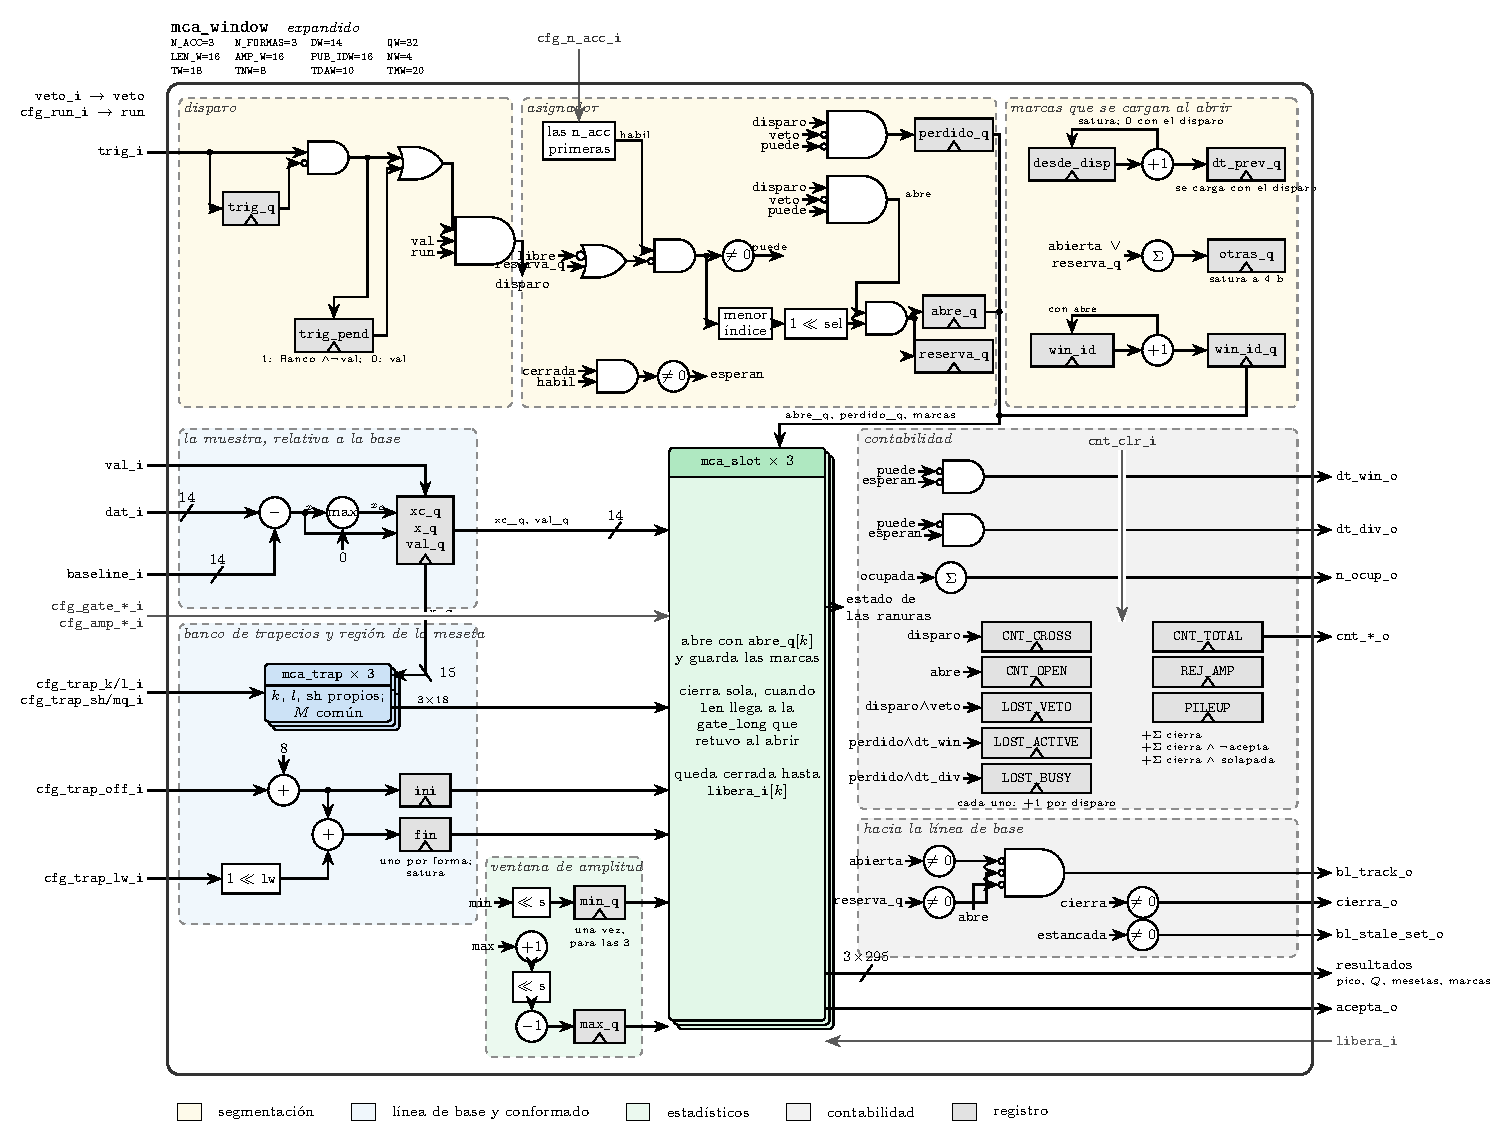
\includegraphics{cap7_panorama_window}
\caption[Vista general de \codigo{mca\_window}]{%
Vista general de \codigo{mca\_window} a nivel de operación. Lo que decide el
asignador se registra en el mismo flanco que la muestra, así que los dos llegan
a la ranura en el mismo ciclo. Ninguna ranura se cierra desde afuera: cada una
cierra cuando su largo llega a la compuerta que retuvo al abrir, y vuelve a
libre cuando el publicador la suelta. A la derecha, la contabilidad.
\codigo{NOMBRE=valor}: parámetros con que lo instancia
\codigo{mca\_pulse\_feature}.\label{f:implmca-window}}
\end{figure}

La contabilidad implementa el \textbf{teselado} de la
Sec.~\ref{S:implmca-teselado}: cada ciclo con \codigo{run} suma en exactamente
un casillero de la Tabla~\ref{t:implmca-teselado}, con la prioridad veto
$>$ \codigo{t\_win} $>$ \codigo{t\_div} $>$ \codigo{t\_rearm} $>$
\codigo{livetime}. Son dos pasos en serie: \codigo{mca\_window} calcula, a
partir del estado de las ranuras, si el módulo puede abrir y, si no puede, por
qué, y \codigo{mca\_top} suma el ciclo al reloj que corresponde. Una ranura
reservada cuenta como ocupada, así que no hay un ciclo en el que el módulo no
pueda abrir y nadie lo cuente.

\subsection{Determinación de estadísticos:
\texorpdfstring{\texttt{mca\_slot}}{mca\_slot}}
\label{S:implmca-slot}

Cada ranura es un juego entero de acumuladores: mide una ventana y, al cerrar,
se queda con el resultado hasta que el publicador lo toma. Así la ranura es a la
vez el lugar donde se mide y un lugar de la cola de publicación. Mientras su
ventana está abierta, actualiza con cada muestra válida las versiones
secuenciales de los estimadores (Sec.~\ref{S:implmca-recuperacion}). En la
Fig.~\ref{f:implmca-slot} se presenta con una fila por acumulador:
\begin{enumerate}
  \item \textbf{Compuertas} (amarillo): al abrir retiene \codigo{gate\_short} y
    \codigo{gate\_long}, así que una ventana mide con lo que se configuró cuando
    abrió, aunque se cambie a mitad de una corrida. \codigo{len} cuenta las
    muestras desde el disparo, y la ranura cierra cuando llega a
    \codigo{gate\_long}. Al cerrar, si la amplitud está dentro de la ventana,
    guarda el resultado hasta que el publicador la libera; si no, se libera sin
    publicar.
  \item \textbf{Pico} (verde): $x_c > \text{pico}$, con comparación estricta: en
    un techo plano gana la primera ocurrencia. Con $\ge$ el instante del pico se
    correría al final de la meseta, y el tiempo al pico saldría arbitrariamente
    largo.
  \item \textbf{Ventana de amplitud} (verde): compara la amplitud, el pico o la
    integral, contra $[\min, \max]$. Se evalúa un ciclo antes del cierre, con
    las restas llevadas en registros sombra, para sacarla del camino crítico.
  \item \textbf{Cargas} (verde): $Q_{tot}$ suma $x_c$ desde la muestra del
    disparo, y $Q_{cola}$ desde la muestra \codigo{gate\_short}, las dos hasta
    el cierre. Al abrir, $Q_{tot}$ arranca con la muestra del disparo y
    $Q_{cola}$ en cero.
  \item \textbf{Meseta, una por forma} (verde): suma la salida del trapecio de
    cada forma mientras la muestra está dentro de la región de su meseta,
    $\text{ini} \le \text{\codigo{len}} < \text{fin}$, y cuenta cuántas sumó. El
    publicador divide esa suma por $2^{lw}$, con un corrimiento de $lw$ bits, y
    obtiene \codigo{F\_TRAP}. Si la cuenta no llegó a $2^{lw}$, porque la
    compuerta cerró antes de terminar la región, publica cero en vez de un
    promedio parcial, que caería en cualquier lugar del espectro: el cero cae en
    el canal 0, donde se ve.
  \item \textbf{Marcas de solape} (gris): \codigo{otras}, \codigo{dt\_prev} y
    \codigo{win\_id} se cargan al abrir. Si llega otro disparo dentro de la
    ventana, se marca \codigo{adentro}, el primero fija \codigo{dt\_next}, y si
    no encontró ranura libre se marca \codigo{perdido}. La ranura no corrige
    nada: deja escrito en el resultado que midió sobre otro pulso.
  \item \textbf{Amplitud} (verde): la integral, $Q_{tot}$ corrida
    \codigo{cfg\_q\_shift} bits y saturada a 16, y la amplitud elegida para la
    ventana, el pico o esa integral.
\end{enumerate}

\begin{figure}[H]
\centering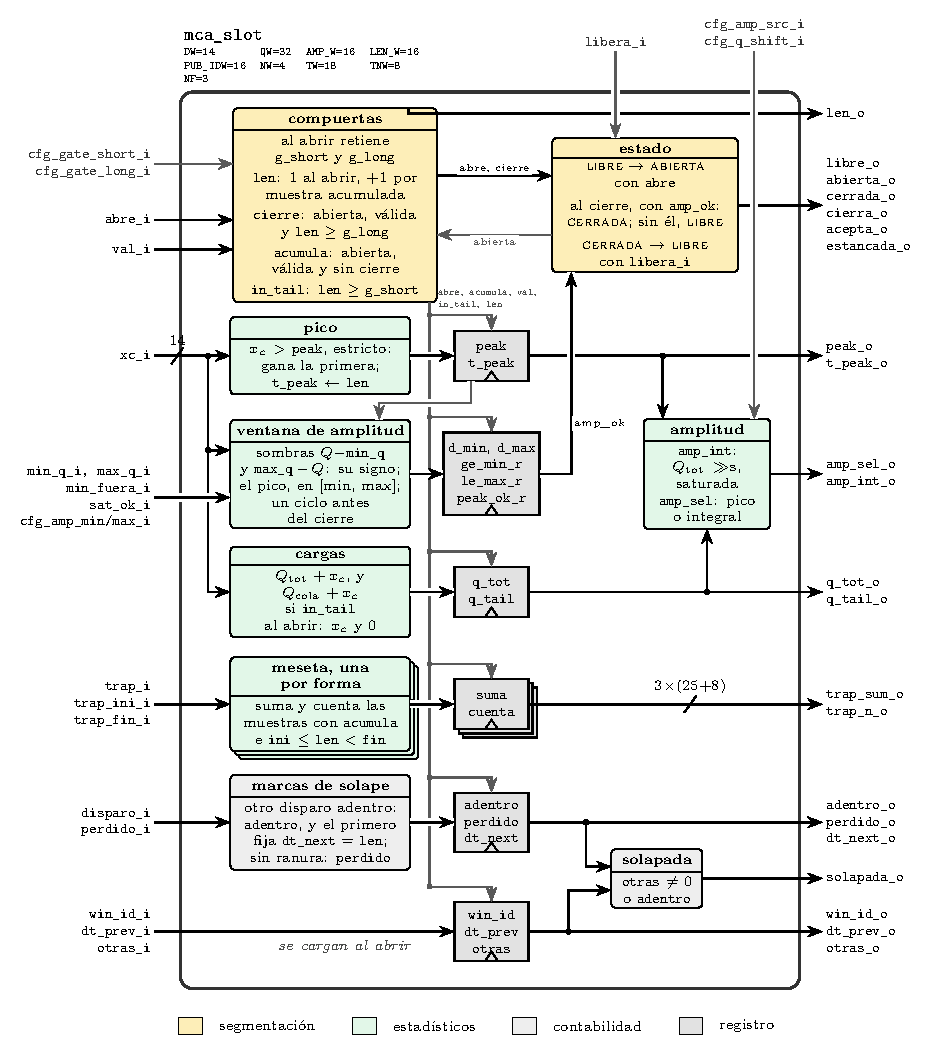
\includegraphics{cap7_panorama_slot}
\caption[Vista general de \codigo{mca\_slot}]{%
Vista general de \codigo{mca\_slot}. Arriba, el control; abajo, una fila por
acumulador: la lógica calcula el valor siguiente y el control elige entre ese,
el de apertura y el que ya tenía. Las marcas de solape no corrigen nada: dejan
escrito en el resultado que se midió sobre otro pulso. \codigo{NOMBRE=valor}:
parámetros con que la instancia \codigo{mca\_window}.\label{f:implmca-slot}}
\end{figure}

Cada ranura suma la meseta de todas las formas del banco en paralelo, porque la
forma recién se puede elegir al cerrar, cuando ya se sabe si llegó otro disparo
dentro de la ventana. En la Fig.~\ref{f:implmca-meseta} se presenta un par de
pulsos visto desde la ranura del primero: la ventana de la forma más corta
termina antes de que llegue el segundo, y en ese momento todavía no se sabe si
las ventanas largas van a quedar limpias.

\begin{figure}[H]
\centering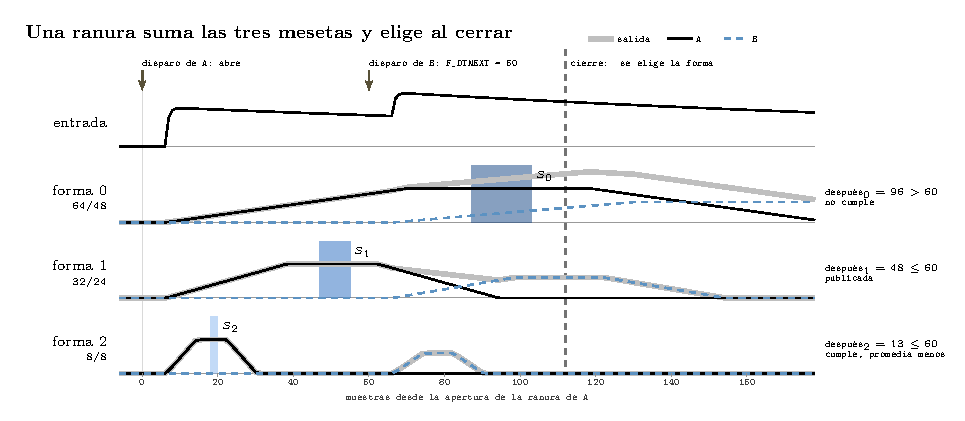
\includegraphics{cap7_meseta_ranura}
\caption[Un par de pulsos visto desde la ranura del primero]{%
Un par de pulsos a 60 muestras visto desde la ranura de A. Hay un trapecio por
forma para toda la señal, y la ranura suma cada uno sobre su ventana ($S_0$ a
$S_2$) mientras su compuerta está abierta. \codigo{F\_DTNEXT} recién es
definitivo al cerrar, y ahí se elige: la 64/48 no cumple, y de las dos que
cumplen se publica la más larga.\label{f:implmca-meseta}}
\end{figure}

\subsection{Publicación a histograma:
\texorpdfstring{\texttt{mca\_publish}}{mca\_publish}}
\label{S:implmca-publish}

El publicador atiende las ranuras cerradas de a una, en el orden en que
cerraron. Los datos del evento no se copian: quedan en su ranura, que no vuelve
a abrir hasta que el publicador la libera. Lo único que hay que guardar es el
orden, y para eso está la \textbf{cola de índices}, una FIFO de
\codigo{N\_ACC} lugares en la que cada lugar tiene el número de una ranura
cerrada. Cuando una ranura cierra, su número entra al final de la cola; si
cierran varias en el mismo ciclo, entran por orden de índice. Cuando el
publicador termina un evento, sale la cabeza y las demás avanzan un lugar. La
cola no puede desbordar, porque cada ranura está en ella a lo sumo una vez. Por
cada evento:
\begin{enumerate}
  \item Guarda en \codigo{cur} el número de la cabeza de la cola y arranca los
    dos divisores, que toman sus operandos de esa ranura. Si la cola estaba
    vacía y el publicador libre, arranca con la ranura que cierra, en el mismo
    flanco del cierre.
  \item En el ciclo en que los divisores toman los operandos, elige la forma
    del banco que se publica en \codigo{F\_TRAP}, así que la elección no agrega
    latencia.
  \item Cuando terminan, carga en un solo flanco las 16 posiciones del bus de
    \emph{features}, lo marca válido durante un ciclo (\codigo{ev\_valid}) y libera la
    ranura.
\end{enumerate}

Cada evento tarda 18 ciclos: el del arranque, el de carga, las 16 iteraciones de
los divisores y el de salida. La latencia no depende del evento, así que el
tiempo que agrega el publicador es siempre el mismo.

La elección de la forma se presenta en la Fig.~\ref{f:implmca-eleccion-forma}.
Por cada forma $f$ (tipo de trapecio en el banco), dos comparaciones dicen si su
ventana queda libre de vecinos: el disparo anterior tiene que estar al menos
$\text{antes}_f$ muestras atrás y el siguiente, al menos $\text{después}_f$
muestras adelante. Entre las formas que cumplen, una prioridad toma la primera,
de la más larga a la más corta, y su suma, dividida por el largo de su ventana,
es \codigo{F\_TRAP}; su índice va a \codigo{F\_FORMA}. Si ninguna cumple, el
pulso queda marcado, con \codigo{F\_TRAP} en cero.

\begin{figure}[H]
\centering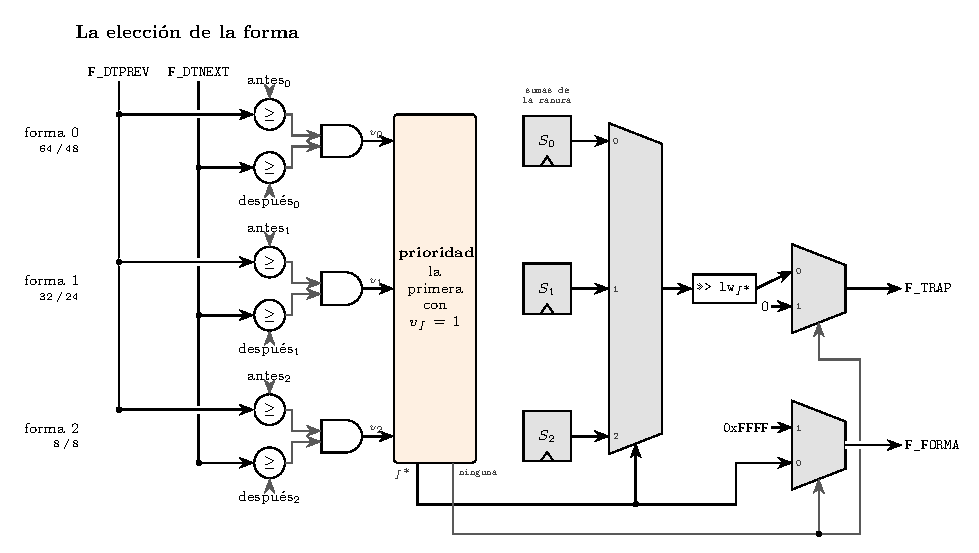
\includegraphics[width=0.75\linewidth]{cap7_eleccion_forma}
\caption[Elección de la forma del banco]{%
La elección de la forma. Por forma, dos comparaciones contra sus umbrales y una
Y; la prioridad toma la primera válida y su índice elige la suma, que el
corrimiento convierte en el promedio sobre la meseta. Si ninguna es válida,
\codigo{F\_TRAP} = 0 y \codigo{F\_FORMA} =
\codigo{0xFFFF}.\label{f:implmca-eleccion-forma}}
\end{figure}

En la Fig.~\ref{f:implmca-bus} se presenta cómo se arma el bus: el resultado de
la ranura que se publica, los cocientes de los divisores y la forma elegida, y
quién lo consume en \codigo{mca\_top}.

\begin{figure}[H]
\centering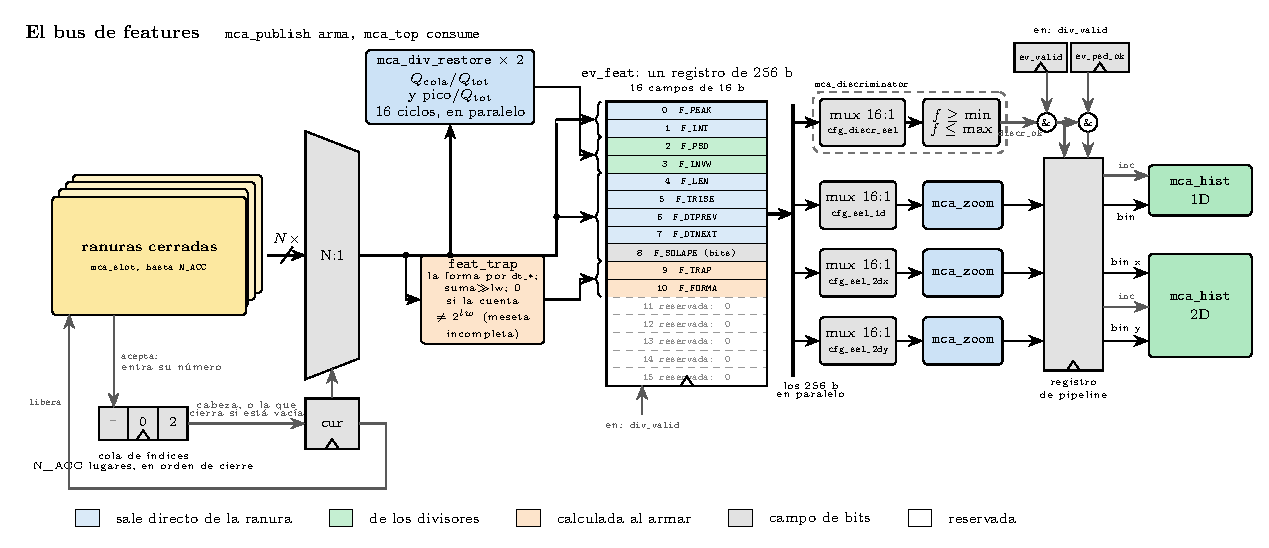
\includegraphics{cap7_bus_features}
\caption[Bus de \emph{features}]{%
Bus de \emph{features}. Cada ranura cerrada guarda su resultado hasta que el publicador
la libera, y la cola de índices guarda el orden en que cerraron (en el ejemplo,
la 2 y después la 0). \codigo{ev\_feat} es un único registro de 256 bits, 16
posiciones de 16 bits que se cargan en el mismo flanco que \codigo{ev\_valid} y
\codigo{ev\_psd\_ok}, así que todo lo que sale es del mismo evento. Las 16
posiciones salen en paralelo, y cada consumidor elige la suya con su propio
multiplexor 16:1, el discriminador incluido.\label{f:implmca-bus}}
\end{figure}

\subsection{Divisor restaurador:
\texorpdfstring{\texttt{mca\_div\_restore}}{mca\_div\_restore}}
\label{S:implmca-div}

Las dos \emph{features} de forma, $Q_{cola}/Q_{tot}$ y $\text{pico}/Q_{tot}$, se
calculan con dos \textbf{divisores restauradores}. Las dos son fracciones entre
0 y 1, y el divisor las entrega como un entero de 16 bits:
\begin{equation}
  q = \left\lfloor \frac{\text{num}}{\text{den}}\, 2^{16} \right\rfloor, \qquad
  \text{num} < \text{den}
  \label{e:implmca-divisor}
\end{equation}
Numerador y denominador son enteros sin signo de 32 bits, tal como salen de la
ranura, y el cociente es una fracción en punto fijo con 16 bits fraccionarios y
sin parte entera (Q0.16): una fracción de 0.5 sale como $2^{15}$, y el cociente
ocupa directamente el rango completo del bus. El divisor restaurador es la
división larga en binario~\citecap{Parhami2010}{13}: saca un bit del cociente
por ciclo, con una comparación y una resta y sin multiplicadores, así que los 16
bits salen en 16 ciclos, sea cual sea el ancho de los operandos.

Los dos divisores trabajan en paralelo, uno por \emph{feature}. Comparten el
denominador $Q_{tot}$ y el arranque, así que el segundo no agrega tiempo. La
latencia es fija, incluso en los casos borde, y eso es deliberado: hace que el
tiempo que tarda el publicador por evento sea siempre el mismo, y con él el
tiempo muerto que agrega. Dividimos $\text{pico}/Q_{tot}$ y no al revés porque
el divisor exige un numerador menor que el denominador, y
$Q_{tot} = \sum x_c \ge \max x_c$ siempre, gracias al recorte a cero.

Los casos borde se tratan aparte. Con $Q_{tot} = 0$ el cociente saldría con
todos los bits en uno, y con $\text{num} \ge \text{den}$ no entraría en 16 bits:
con $\text{num} = \text{den}$, por ejemplo, daría $2^{16}$, que se envuelve a
cero. En los dos casos el evento caería en un extremo del eje sin aviso. En
lugar de eso, si $Q_{tot} = 0$ o $Q_{cola} \ge Q_{tot}$, la forma se marca como
inválida (\codigo{cnt\_rej\_psd}): el evento entra al 1D, pero no al 2D. El
ancho inverso sólo llega a 1 con un pulso de una sola muestra, y en ese caso
satura en \codigo{0xFFFF}.

\subsection{Módulo de \emph{zoom}:
\texorpdfstring{\texttt{mca\_zoom}}{mca\_zoom}}
\label{S:implmca-zoom}

Antes del \emph{zoom}, un mux 16:1 por eje elige qué \emph{feature} del bus va a ese eje
(\codigo{cfg\_sel\_1d}, \codigo{cfg\_sel\_2dx} y \codigo{cfg\_sel\_2dy}), con la
numeración de la Tabla~\ref{t:implmca-estimadores}. El \emph{zoom} le asigna a esa
\emph{feature} el índice del bin. La ventana del eje es
$\left[k\,2^{16-z},\ (k+1)\,2^{16-z}\right)$, con $z$ el nivel de \emph{zoom} y $k$ el
índice de la ventana, $0 \le k < 2^z$, como se presenta en la
Fig.~\ref{f:implmca-zoom}. Con $z = 0$, que es el valor de \emph{reset}, la ventana es
el rango completo de la \emph{feature}, y el bin son sus bits más altos. La ventana
empieza en un múltiplo de su ancho, y su ancho es una potencia de dos. Así la
cuenta es sólo de bits: la \emph{feature} está adentro si sus $z$ bits más altos valen
$k$, y el bin son los bits siguientes, sin restar ni multiplicar. Además, los
bins de un nivel son subdivisiones exactas de los del anterior: un bin de nivel
$z$ es la suma de dos de nivel $z+1$. Por eso espectros tomados con \emph{zoom}
distinto se combinan sumando enteros, sin re-muestrear.

Un evento fuera de la ventana satura: va al último bin si está por encima y al
primero si está por debajo, así que los bins de los extremos avisan del
desborde. El \emph{zoom} no mejora la resolución: sólo achica la pérdida por bineado
(Sec.~\ref{S:implmca-fisher-bineado}). Sirve para ubicar el eje sobre una región
de interés y para poder usar un histograma más chico.

\begin{figure}[H]
\centering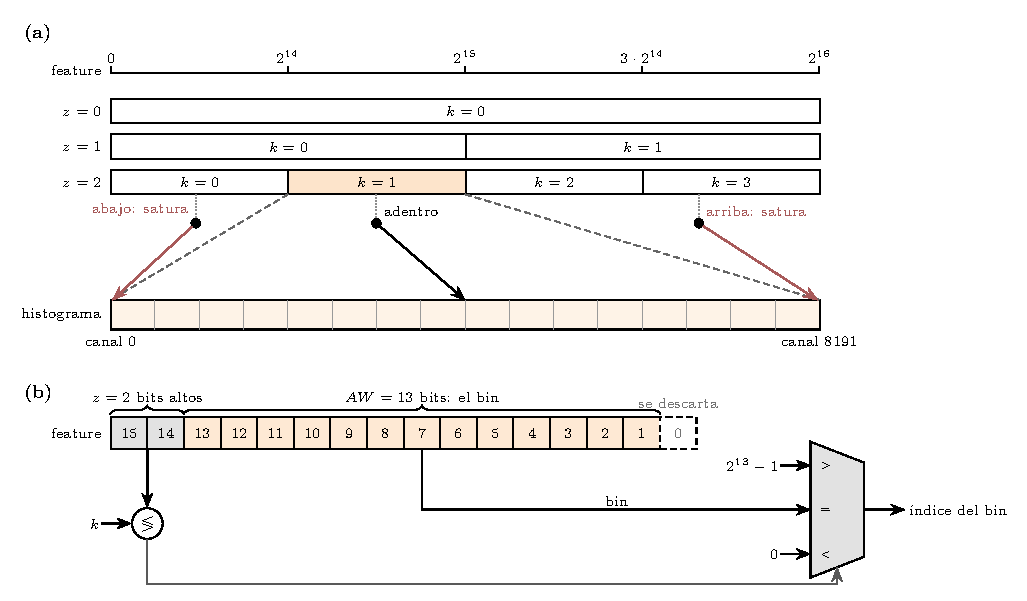
\includegraphics{cap7_zoom_ventanas}
\caption[El \emph{zoom} de un eje del histograma]{%
El \emph{zoom} de un eje, para el espectro 1D (\emph{feature} de 16 bits, 8192 canales). (a)
En el nivel $z$ el rango de la \emph{feature} se parte en $2^z$ ventanas iguales y
alineadas, y la ventana $k$ ocupa el histograma entero. Con $z = 2$ y $k = 1$,
un evento adentro cae en el bin proporcional, y los de afuera saturan en el
primer y en el último canal. (b) La misma cuenta en bits: los $z$ bits altos se
comparan con $k$, los 13 siguientes son el bin y el resto se
descarta.\label{f:implmca-zoom}}
\end{figure}

\subsection{Discriminador:
\texorpdfstring{\texttt{mca\_discriminator}}{mca\_discriminator}}
\label{S:implmca-discr}

Acepta o rechaza el evento según una \emph{feature} del bus, elegida con
\codigo{cfg\_discr\_sel}. Con \codigo{cfg\_discr\_out = 0} acepta si la \emph{feature}
está en $[\min, \max]$, y con \codigo{cfg\_discr\_out = 1}, si está afuera;
deshabilitado, acepta todo. Con $\min > \max$ el intervalo es vacío, así que
rechaza todo o acepta todo, según el modo. Un evento rechazado no va a ninguno
de los dos histogramas y se cuenta en \codigo{cnt\_rej\_discr}.

Está después de los divisores para que pueda mirar las \emph{features} de forma, que no
existen hasta que el divisor termina: un corte en $\text{pico}/Q_{tot}$ separa
los pulsos apilados, que son más anchos, de los limpios. El costo es que todo
evento paga la latencia del publicador antes de poder ser rechazado.

\subsection{Módulo de histograma:
\texorpdfstring{\texttt{mca\_hist}}{mca\_hist}}
\label{S:implmca-hist}

Cada histograma es una memoria de $2^{AW}$ contadores de 32 bits, en una BRAM de
doble puerto simple: un puerto sólo escribe y el otro sólo lee. El 1D tiene 8192
canales y el 2D, $128 \times 64$ bines. Un incremento es una lectura, una suma y
una escritura en tres etapas: en el ciclo $m$ lee el bin, en $m+1$ calcula el
valor nuevo y en $m+2$ lo escribe. Con la lectura y la escritura en puertos
distintos acepta un incremento por ciclo. Si dos eventos seguidos caen en el
mismo bin, el segundo leería un valor viejo; por eso el valor se toma
directamente de las dos escrituras en vuelo (\emph{forwarding}) cuando la
dirección coincide.
\begin{itemize}
  \item \textbf{Lectura del bus}: tiene prioridad sobre el incremento en el
    puerto de lectura. Un incremento que llega en ese ciclo se pierde y se
    cuenta en \codigo{dropped}.
  \item \textbf{Borrado}: un barrido de $2^{AW}$ ciclos que usa sólo el puerto
    de escritura, así que el bus puede seguir leyendo mientras se borra. Los
    incrementos que llegan durante el barrido también van a \codigo{dropped}, y
    los que estaban en vuelo se descartan, para no dejar cuentas en un
    histograma recién borrado.
  \item \textbf{Lleno}: los contadores saturan en $2^{32} - 1$. El primer bin
    que llega al tope levanta \codigo{full}, que queda hasta el próximo borrado;
    con \codigo{cfg\_keep\_full = 0} se congela el histograma entero y los
    incrementos siguientes van a \codigo{cnt\_full\_supp}
    (Sec.~\ref{S:implmca-flujo}).
\end{itemize}

% Bibliografía de este capítulo. Va al final del archivo, siempre.
\bibliografiacapitulo

%%% Local Variables:
%%% mode: latex
%%% TeX-master: "template"
%%% End:
       % Implementación del MCA (señuelo)
% Origen: Secciones/PI - Resultados de Merito.md (antes "... Merito MCA")
% (antes "PI - Resultados de Monte-Carlo, Validacion y Mediciones"). La parte de
% Monte-Carlo quedó en otra nota, "PI - Resultados Monte - Carlo.md", todavía
% sin convertir: por eso S:res-montecarlo sigue pendiente en cap4.
\chapter{Resultados de mérito}
\label{C:resultados}

% Figuras de ESTE capítulo + las compartidas. Siempre al principio del archivo.
\graphicspath{{figs/cap9/}{figs/comunes/}}

\begin{destacado}
En este capítulo se presentan resultados de mediciones mediante la generación
interna y posterior canalización a un lazo analógico del módulo MCA.
\end{destacado}

%==============================================================================
\section{Etapas de experimentos y validación}
\label{S:res-etapas-validacion}

Esto es aislar las dependencias en la cadena de adquisición; en particular
identificamos las siguientes:
\begin{itemize}
  \item \textbf{Simulación} (Monte-Carlo):
  \begin{itemize}
    \item Completamente computacional.
    \item No necesariamente contiene detalles de la implementación del HW.
  \end{itemize}
  \item \textbf{Verificación}: simulaciones de comprobación de la respuesta del
    HW.
  \begin{itemize}
    \item Nuestros estímulos se realizan mediante asignaciones directas a las
      señales de entrada de un módulo; estas operaciones no son sintetizables.
    \item Estos resultados se presentan en las secciones de verificación de los
      módulos individuales, por ejemplo la Sec.~\ref{S:ap-mt-verificacion}.
  \end{itemize}
  \item \textbf{Generación interna}:
  \begin{itemize}
    \item Ya estamos de forma completa en HW.
    \item Medimos en HW una salida generada por el mismo HW. Un ejemplo de la
      misma se encuentra en la
      Fig.~\ref{f:top-datapath}.
    \item La señal generada tendrá las propiedades que nosotros deseamos: vamos
      a tener una emisión de un comando de generación y vamos a ver la salida de
      nuestros módulos a la misma.
  \end{itemize}
  \item \textbf{Generación externa controlada}:
  \begin{itemize}
    \item Los comandos de generación se transmiten a un elemento externo, como
      un generador de pulsos, y la salida de este se conecta a nuestro HW por
      una interfaz rápida. Esto se presenta en la
      Fig.~\ref{f:res-setup-externo}.
  \end{itemize}
  \item \textbf{Medición con \emph{setup} experimental}: utilizamos un medidor con
    física real.
\end{itemize}

%==============================================================================
\section{Resultados de generación externa controlada}
\label{S:res-gen-externa}

Este fue el primer sistema de medición real que implementamos. Conectamos las
dos entradas analógicas de alta velocidad a los dos canales de salida del
generador de ondas Rigol DG-4162. Ambas conexiones utilizaban un coaxial
KingSignal RG-58 con conectores macho SMA en las terminales de la Pitaya y
conector BNC en la terminal del Rigol. El Rigol se controló por su puerto
trasero del tipo USB-Host, manejado por la Pitaya; la comunicación se realizó
mediante el protocolo especializado Rigol USB TMC \emph{Driver}. En la
Fig.~\ref{f:res-setup-externo} se presenta de forma esquemática el \emph{setup};
mediante \codigo{ssh} teníamos control de los \emph{scripts} de testeo.

\begin{figure}[H]
\centering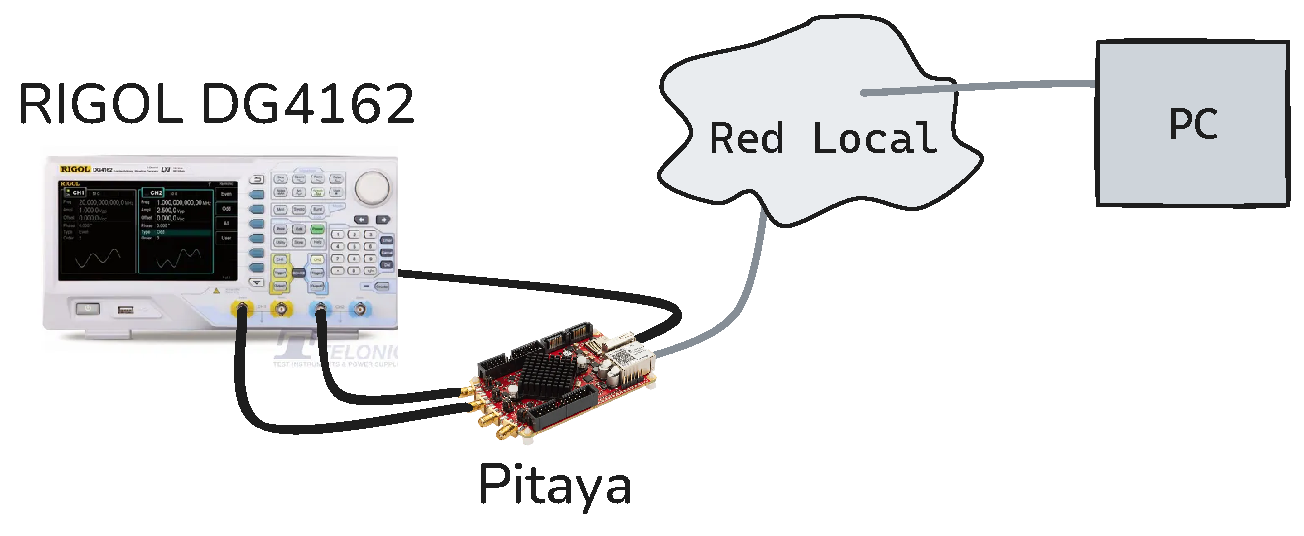
\includegraphics{cap9_setup_externo}
\caption[Esquema de verificación inicial]{%
Esquema de verificación inicial.\label{f:res-setup-externo}}
\end{figure}

Aún así, este sistema cuenta con las siguientes limitaciones:
\begin{itemize}
  \item Techo de \emph{throughput}: la generación de pulsos con este sistema
    tiene como límite 794~kEv/s.
  \item No separa la INL del generador de la del ADC: la entrada es la cascada
    de los dos sistemas.
\end{itemize}
Para superar estas limitaciones pasamos a la configuración de generación
interna.

\subsection{\emph{Setup} de generación interna}
\label{S:res-setup-interna}

La versión más simple de realizarla es mediante el lazo interno a la PL:
ponemos en la entrada de nuestros medidores la salida de un módulo que genera
estímulos controlados (\codigo{gen\_pulsos}), y a esto lo llamamos \textbf{lazo
digital}. El \textbf{lazo analógico}, en cambio, canaliza la salida del ASG al
OUT1 de la Pitaya, que se conecta a IN1. En este caso testearíamos el sistema
anterior más los efectos producidos por los front-end analógicos, el ADC, el
DAC, las terminaciones SMA y el cable coaxial. Este \emph{setup} se puede observar en
la Fig.~\ref{f:res-conexion-in-out}.

\begin{figure}[H]
\centering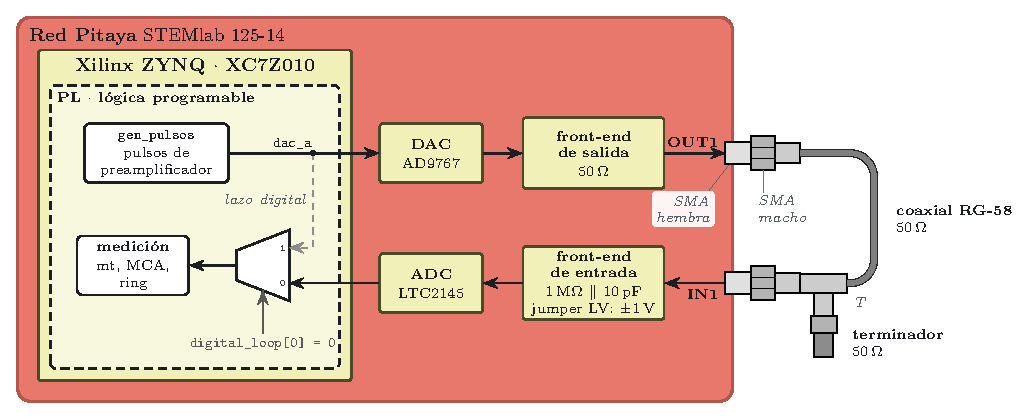
\includegraphics{cap9_conexion_in_out}
\caption[\emph{Setup} de generación interna]{%
\emph{Setup} de generación interna. Se puede emplear \codigo{digital\_loop=1} para que
la señal se genere y se consuma dentro del \emph{fabric} de la PL, o se puede utilizar
\codigo{digital\_loop=0} para hacer uso de la entrada analógica \codigo{IN1}, en
este caso conectada directamente desde OUT1 con un conector T y una carga de
\qty{50}{\ohm}.\label{f:res-conexion-in-out}}
\end{figure}

Conectamos OUT1 a IN1 con una T y una carga de \qty{50}{\ohm} porque, si no, se
presentaban los armónicos lentos en \qty{12.3}{\mega\hertz},
\qty{34.7}{\mega\hertz} y \qty{53.2}{\mega\hertz} mostrados en la
Fig.~\ref{f:res-canal}(b), que es la transferencia para OUT2 $\rightarrow$ IN2
sin compensación. Para el resto de las pruebas se utilizó el canal
OUT1 $\rightarrow$ IN1 adaptado.

\begin{figure}[H]
\centering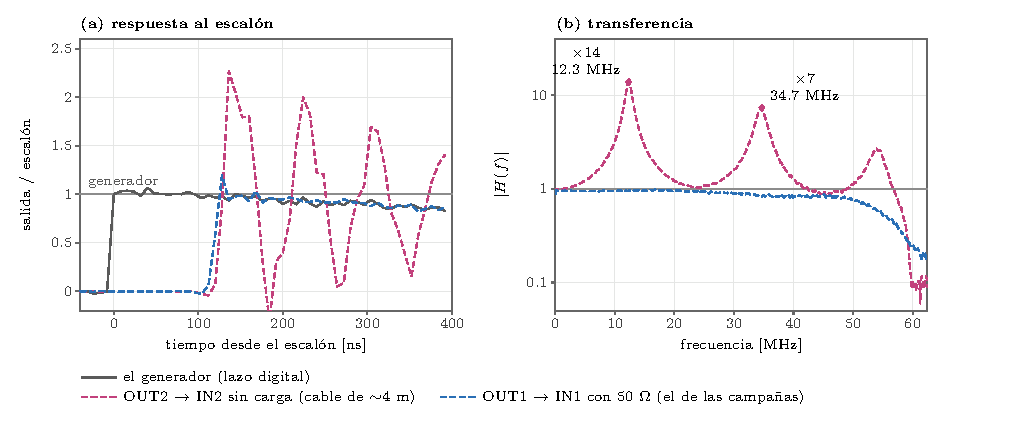
\includegraphics{cap9_canal_analogico}
\caption[El canal analógico medido con la BRAM]{%
El canal analógico medido con la BRAM: el mismo estímulo capturado con el lazo
digital (el generador) y sin él. (a) Respuesta a un escalón de 1727~ADU,
normalizada; (b) transferencia $|H(f)|$ por espectros cruzados
(Welch).\label{f:res-canal}}
\end{figure}

\begin{destacado}
Las amplitudes no las expresamos en tensión sino en \textbf{ADU}
(\emph{analog-to-digital units}), el escalón del código de 14 bits. Las
posiciones en el histograma (centroides y corrimientos) van en
\textbf{canales}.
\end{destacado}

%==============================================================================
\section{Resultados de generación interna}
\label{S:res-gen-interna}

Una vez comprobado el funcionamiento correcto de la fuente de pulsos comenzamos
a realizar diversas pruebas; en la Tabla~\ref{t:res-setup} se presenta la
configuración del MCA en las mediciones. Se denominan \textbf{pulsos buenos} los
estimados dentro de un rango de \qty{2}{\percent} de error.

% La tabla no tiene epígrafe en la nota y la frase que la presenta quedó
% cortada ("en la Tabla{prueba_setup_original} las mediciones ."): el epígrafe
% y el "se presenta la configuración del MCA" son provisorios.
\begin{table}[H]
\centering
\caption[Configuración del MCA en las mediciones]{%
Configuración del MCA en las mediciones de generación
interna.\label{t:res-setup}}
\begin{tabularx}{\textwidth}{|l|>{\raggedright\arraybackslash}X|}
\hline \encabezado \textbf{Parámetro} & \textbf{Valor} \\ \hline
Espectro 1D & 8192 canales (\codigo{H\_AW} = 13), contadores de 32 bits que
  saturan \\ \hline
Mapa 2D & $128 \times 64$ canales (amplitud $\times$ forma) \\ \hline
Ranuras de medición & 3 (\codigo{N\_ACC}) \\ \hline
Formas del banco de trapecios & 3 (\codigo{N\_FORMAS}) \\ \hline
\end{tabularx}
\end{table}

\subsection{Comparación de la tasa de medición obtenida vs.\ la excitada}
\label{S:res-tasa}

Para medir la tasa de eventos, hicimos un barrido de la tasa de entrada de
10~k/s a 3~M/s. Los arribos son de Poisson, con dos líneas de 500 y 1300
cuentas (60/40) y $\tau = \qty{2}{\micro\second}$. Los resultados con el ASG y
de 1 a 3 ranuras se presentan en la Fig.~\ref{f:res-tasa}. Con 3 ranuras y
3~M/s de entrada, el MCA acepta 1.9~M/s y entrega 1.2~M/s buenos.

\begin{figure}[H]
\centering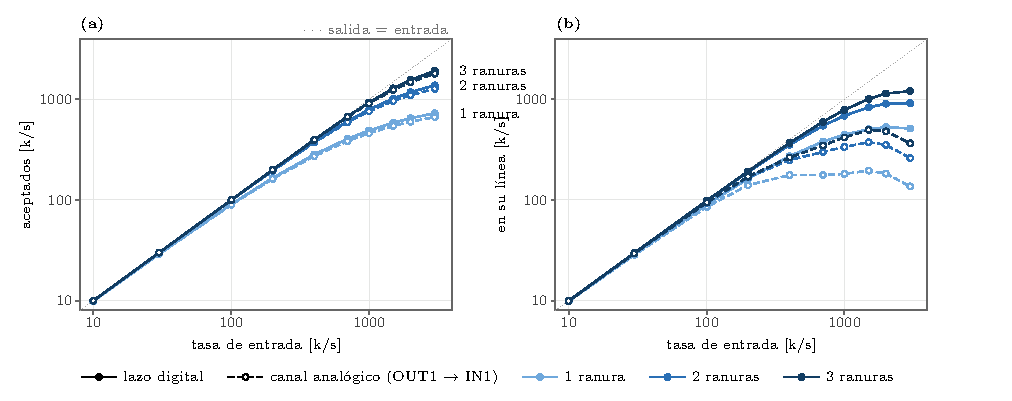
\includegraphics{cap9_meritos_tasa}
\caption[Tasa de eventos del MCA contra la cantidad de ranuras]{%
Tasa de eventos del MCA con \codigo{gen\_pulsos} (Poisson, líneas de 500 y
1300~ADU, disparo por el ASG, trapecio). (a) Eventos aceptados por segundo y
(b) eventos en su línea (a $\pm\qty{2}{\percent}$ del centroide de su línea de
referencia) por segundo, contra la tasa de entrada, con 1, 2 y 3 ranuras. Línea
llena: lazo digital; a trazos: canal analógico OUT1 $\rightarrow$ IN1 con
\qty{50}{\ohm}.\label{f:res-tasa}}
\end{figure}

\textbf{En el canal analógico los aceptados casi no cambian, pero la tasa en la
línea cae.}

Si realizamos la misma medición pero cambiando las fuentes de disparo obtenemos
la Fig.~\ref{f:res-tasa-fuentes}.

\begin{figure}[H]
\centering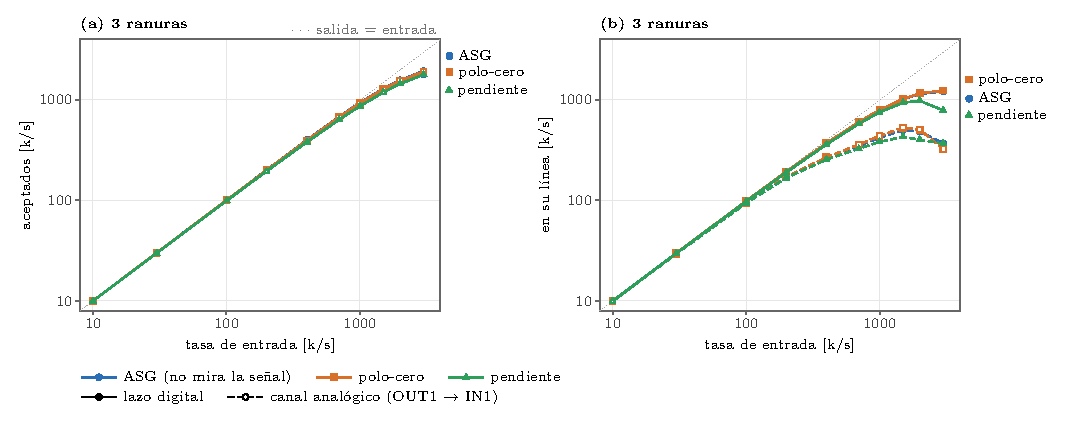
\includegraphics{cap9_meritos_tasa_fuentes}
\caption[Tasa de eventos con cada fuente de disparo]{%
Tasa de eventos con cada fuente de disparo (Poisson, líneas de 500 y 1300~ADU,
disparo por el ASG, trapecio). (a) Eventos aceptados y (b) eventos en su línea
(a $\pm\qty{2}{\percent}$ del centroide de su línea de referencia) por segundo,
contra la tasa de entrada. Línea llena: lazo digital; a trazos: canal analógico
OUT1 $\rightarrow$ IN1 con \qty{50}{\ohm}.\label{f:res-tasa-fuentes}}
\end{figure}

El ASG refiere a la salida del generador de pulsos que indica cuándo un pulso
sale del sistema; un \emph{trigger} ideal debería ser igual a esta ciclo a ciclo (a
menos de un retardo fijo).

\subsection{Error de tasa estimada}
\label{S:res-error-tasa}

En la Sec.~\ref{S:res-tasa} vimos la \textbf{tasa medida}; ahora podemos aplicar
sobre esta una compensación para obtener un \textbf{estimador de la tasa real}
$\hat\lambda$. Este mecanismo se presenta en el Cap.~\ref{C:implmca}.
A esta la comparamos con la tasa exacta del generador. Los resultados se
presentan en la Fig.~\ref{f:res-lambda}, como error relativo en \%, con 1
ranura en (a) y 3 ranuras en (b).

\begin{figure}[H]
\centering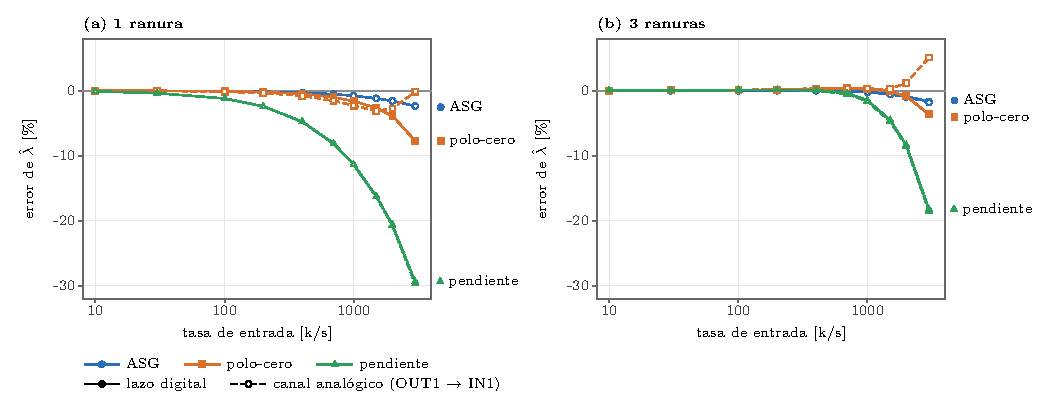
\includegraphics{cap9_meritos_lambda}
\caption[Error de la tasa estimada por el MCA]{%
Error de la tasa estimada por el SW del MCA medida contra la tasa del
generador.\label{f:res-lambda}}
\end{figure}

\subsection{Medición de la resolución de pico en función del ruido}
\label{S:res-ruido}

Para medir la resolución de cada estimador, hicimos un barrido de la varianza
del ruido blanco que suma \codigo{gen\_pulsos}, de 0 a 148~ADU de $\sigma$
(\codigo{ruido\_sh} de 8 a 0). La línea es de 1500~ADU, con 4000 pulsos por
punto. Usamos el disparo del ASG, que no depende del ruido. Ajustamos la curva
\begin{equation}
  \sigma^2 = (g\,\sigma_\text{ruido})^2 + \sigma_0^2 ,
  \label{e:res-ruido}
\end{equation}
donde definimos $g$ como la ganancia de ruido del estimador y $\sigma_0$ como el
ruido de fondo. Los resultados se presentan en la Fig.~\ref{f:res-ruido}, con
los dos ejes logarítmicos.

\begin{figure}[H]
\centering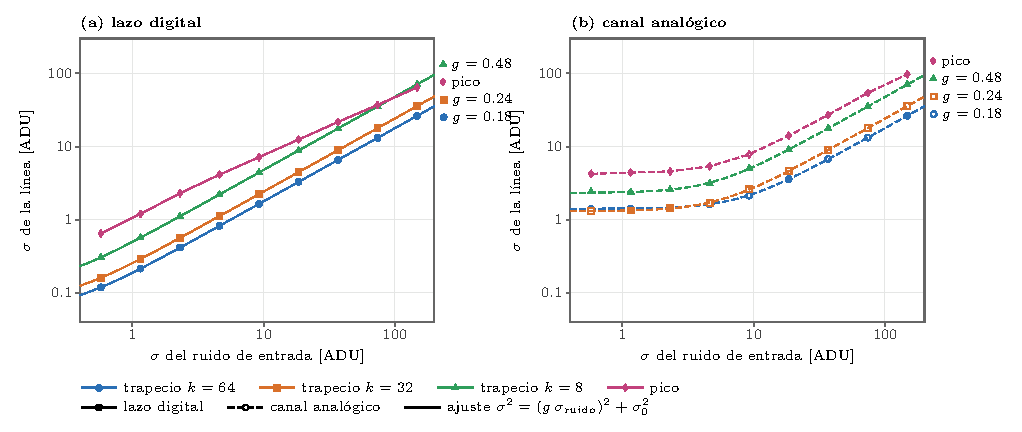
\includegraphics{cap9_meritos_ruido}
\caption[Resolución de cada estimador contra el ruido blanco]{%
Resolución de cada estimador contra el ruido blanco que suma
\codigo{gen\_pulsos} (línea de 1500~ADU, disparo por el ASG, 4000 pulsos por
punto): $\sigma$ de la línea, en ADU, contra el $\sigma$ del ruido de entrada.
Las curvas son el ajuste
$\sigma^2 = (g\,\sigma_\text{ruido})^2 + \sigma_0^2$.\label{f:res-ruido}}
\end{figure}

La ganancia de ruido $g$ baja con la subida $k$ del trapecio como $1/\sqrt{k}$
(0.48, 0.24 y 0.18 para $k = 8$, 32 y 64) y es la misma en los dos modos; el
canal analógico agrega el piso $\sigma_0$ del ADC.

% Desde acá las figuras van con [H]: el texto es corto y como floats se
% acumulaban al final del capítulo, solas en sus páginas.
\subsection{Medición de la resolución de par de pulsos y sobreestimación de
  pulsos}
\label{S:res-par}

Para medir la resolución de pulsos dobles, generamos pares de 4000 y 2400
cuentas y barrimos la separación $\Delta t$ entre ellos de 2 a 512 ciclos de
\qty{8}{\nano\second}, con 2000 pares por punto. Con 1 ranura, los dos pulsos
salen bien recién desde $\Delta t = 192$. La resolución fija la ranura: el
segundo pulso tiene que esperar a que se libere. En el canal analógico, la
pendiente se comporta igual. El polo-cero, en cambio, vuelve a disparar sobre el
sobrepico del \qty{24}{\percent}, con hasta 3.8 disparos por par, y casi nunca
deja los dos pulsos buenos (Fig.~\ref{f:res-par}).

\begin{figure}[H]
\centering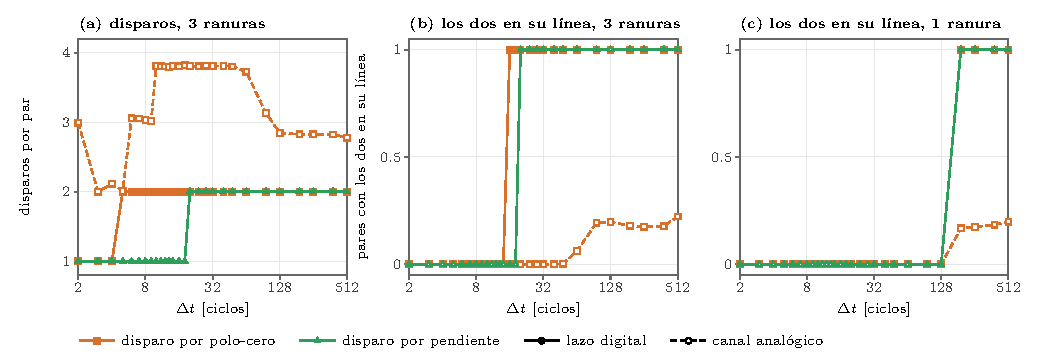
\includegraphics{cap9_meritos_par}
\caption[Resolución de pulsos dobles]{%
Resolución de pulsos dobles: pares de 4000 y 2400~ADU separados $\Delta t$
ciclos de \qty{8}{\nano\second}, 2000 pares por punto. (a) Disparos por par;
(b) fracción de pares en que el trapecio mide los dos pulsos en su línea
($\pm\qty{2}{\percent}$) con 3 ranuras y (c) con 1 ranura.\label{f:res-par}}
\end{figure}

\subsection{Medición del corrimiento del centroide}
\label{S:res-corrimiento}

Para el mismo barrido de tasa comparamos la posición del centroide emitido con
el medido, en búsqueda de \textbf{desviaciones sistemáticas}. Los resultados se
presentan en la Fig.~\ref{f:res-corrimiento}, con una curva por línea.

\begin{figure}[H]
\centering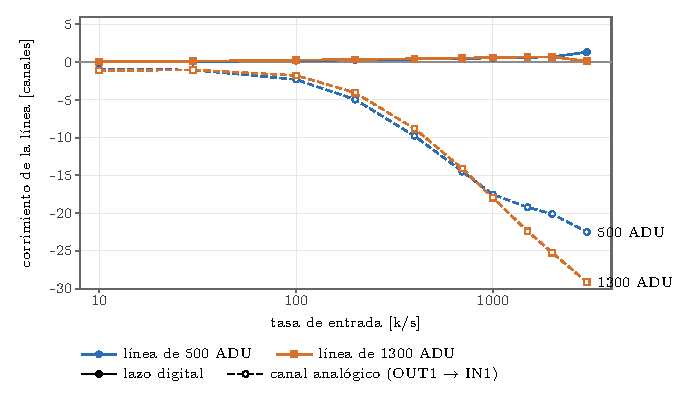
\includegraphics{cap9_meritos_corrimiento}
\caption[Corrimiento del centroide contra la tasa de entrada]{%
Corrimiento del centroide de cada línea contra la tasa de entrada (trapecio,
ASG, 3 ranuras, base fija). En el lazo digital no tenemos corrimiento
apreciable hasta 1~MEv/s, donde se vuelve menor de 2
canales.\label{f:res-corrimiento}}
\end{figure}

En el lazo digital las líneas no se mueven más de 2 canales; el canal analógico,
por otro lado, tiene un error que sigue la misma ecuación que vimos antes
\incompleto{} (falta la ecuación del error). Aún así, este elemento no es
corregible porque no es interno a nuestro módulo. Nos habla de la transferencia
analógica del canal. Por esta razón se recomienda
realizar esta medición previa para obtener la curva de respuesta del
corrimiento y poder compensar de forma automática según los valores obtenidos.
Es importante, igualmente, utilizar el mismo conexionado del \emph{setup} con el que
estemos trabajando, pero en vez de utilizar como salida el sensor, conectar a
OUT1.

\begin{destacado}
Estas \textbf{desviaciones se explican por el apilamiento} sobre las colas
negativas que deja la caída lenta del canal: la base baja con la tasa, y el
trapecio con polo-cero pasa ese error a la amplitud en $(k + m)/\tau$, igual
para todas las alturas hasta $\sim$1~M/s, donde el banco pasa a las formas
cortas.
\end{destacado}

\subsection{Medición de la no linealidad integral (INL) del conformado
  trapezoidal}
\label{S:res-inl-trapecio}

Con los mismos pulsos aislados medimos la línea del trapecio en cada amplitud.
Ajustamos una recta entre 200 y 3200~ADU, donde nada satura, y calculamos el
residuo en \% del fondo de escala (8191~ADU). Los resultados se presentan en la
Fig.~\ref{f:res-inl}. En el lazo digital, el residuo es menor que
\qty{0.002}{\percent}~FS (0.16~ADU) en todo el rango.

\begin{figure}[H]
\centering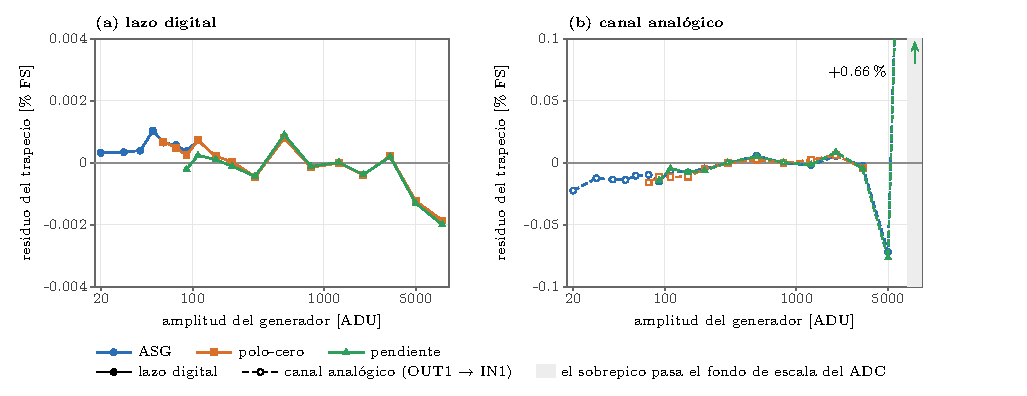
\includegraphics{cap9_meritos_inl}
\caption[No linealidad integral del trapecio]{%
No linealidad integral del trapecio, con cada fuente de disparo: el residuo de
la línea de pulsos aislados (400 por amplitud) contra una recta ajustada entre
200 y 3200~ADU, en \% del fondo de escala (8191~ADU). (a) Lazo digital, (b)
canal analógico.\label{f:res-inl}}
\end{figure}

El polo-cero no tiene línea desde 5000~ADU, porque vuelve a disparar sobre el
sobrepico; este efecto de disparo se presenta en la Sec.~\ref{S:res-walk}.

\subsection{Medición del \emph{walk} de disparo}
\label{S:res-walk}

Para medir el umbral y el \emph{walk} de cada fuente de disparo, barrimos la amplitud
de pulsos aislados de 20 a 8000~ADU, con 400 pulsos por punto y un ruido de
2.3~ADU. Los resultados se presentan en la Fig.~\ref{f:res-walk}. En cada punto
medimos tres cosas. La curva del panel (a) da la fracción de pulsos que disparan
y nos dice el umbral efectivo a utilizar. El polo-cero dispara la mitad de los
pulsos en 48~ADU y la pendiente en 81. En el canal analógico, 51 y 82: el canal
casi no mueve el umbral. El panel (b) es el \emph{walk}, el retardo del disparo, a
partir de \codigo{t\_subida}. El polo-cero se atrasa 1 ciclo
(\qty{8}{\nano\second}) con los pulsos chicos y la pendiente 6 ciclos
(\qty{48}{\nano\second}). En el canal analógico, 2 y 6.9 ciclos. En el panel
(c) están los disparos por pulso: el ASG dispara una vez siempre, porque no mira
la señal. En el canal analógico, el polo-cero vuelve a disparar \textbf{sobre el
sobrepico desde unas 3200~ADU}.

\begin{figure}[H]
\centering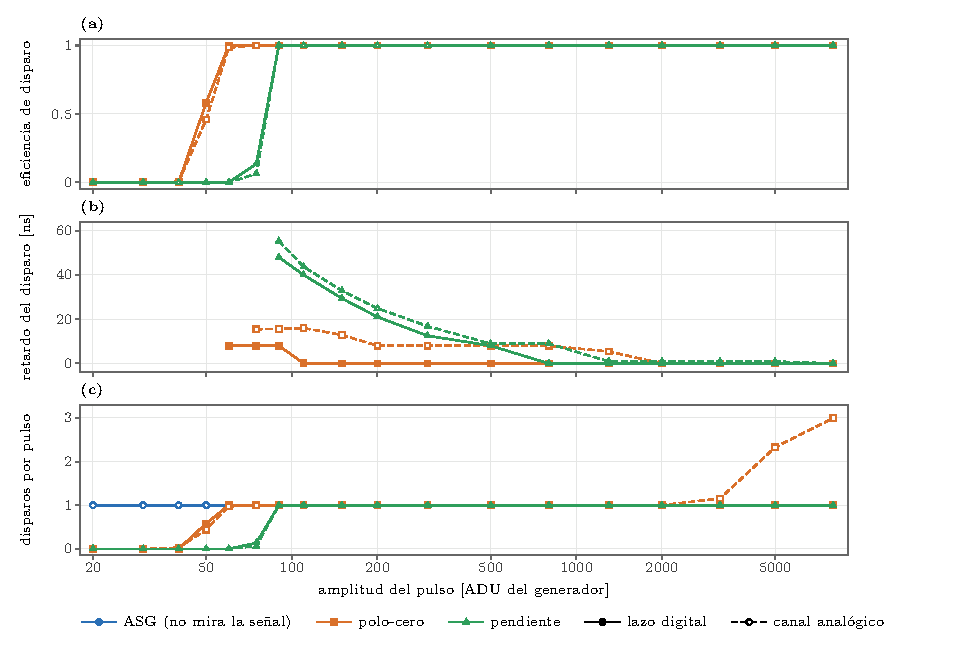
\includegraphics{cap9_meritos_walk}
\caption[El disparo contra la amplitud de un pulso aislado]{%
El disparo contra la amplitud de un pulso aislado (400 pulsos por punto, ruido
de 2.3~ADU). (a) Fracción de pulsos que disparan, (b) retardo del disparo, en
ciclos de \qty{8}{\nano\second}, (c) disparos por pulso.\label{f:res-walk}}
\end{figure}

\subsection{Medición de la DNL (no linealidad diferencial)}
\label{S:res-dnl}

Para medir la DNL, generamos alturas uniformes de 500 a 5615~ADU, en pasos de
5~ADU, con ruido $\sigma = 18.5$~ADU por muestra como \emph{dither}. Para que no
haya apilamiento, usamos pulsos de $\tau = 50$ muestras cada 300 ciclos,
12.5~M pulsos en total. La DNL de cada canal es cuánto se apartan sus cuentas de
la meseta, y la comparamos con la que da la estadística de Poisson con esas
cuentas. Los resultados se presentan en la Tabla~\ref{t:res-dnl}.

\begin{table}[H]
\centering
\caption[DNL de cada espectro con alturas uniformes]{%
DNL rms de cada espectro con alturas uniformes de 500 a 5615~ADU, contra la que
da la estadística de Poisson con esas cuentas por canal. El pico usa un canal
por ADU.\label{t:res-dnl}}
\begin{tabular}{|l|c|c|c|c|}
\hline \encabezado \textbf{Espectro} & \textbf{Cuentas por canal} &
  \textbf{DNL rms} & \textbf{Poisson} & \textbf{Máximo} \\ \hline
Trapecio, lazo digital    & 3095 & \qty{1.76}{\percent} & \qty{1.80}{\percent}
  & \qty{6.6}{\percent} \\ \hline
Pico, lazo digital        & 2445 & \qty{2.03}{\percent} & \qty{2.02}{\percent}
  & \qty{8.2}{\percent} \\ \hline
Trapecio, canal analógico & 3258 & \qty{1.76}{\percent} & \qty{1.75}{\percent}
  & \qty{5.8}{\percent} \\ \hline
Pico, canal analógico     & 2113 & \qty{3.41}{\percent} & \qty{2.18}{\percent}
  & \qty{15.0}{\percent} \\ \hline
\end{tabular}
\end{table}

En el lazo digital, el trapecio y el pico quedan en la estadística: el MCA no
agrega DNL. En el canal analógico el trapecio también, pero el pico, con un
canal por código del ADC, da \qty{3.41}{\percent} contra \qty{2.18}{\percent}:
un código de cada dos es \qty{3}{\percent} más ancho que el otro. El trapecio no
lo ve, porque promedia muchas muestras de cada pulso.

\subsection{Sensibilidad al ajuste del polo-cero}
\label{S:res-polo-cero}

Para ver cuánto importa la $M$ del polo-cero del trapecio, generamos pares de
4000 y 2400~ADU separados $\Delta t = 100$, 200 y 400 ciclos, con $\tau = 250$
muestras, y corrimos la $M$ del trapecio $\Delta M$ entre $-10$ y
$+\qty{10}{\percent}$ de la del generador. El segundo pulso cae sobre la cola
del primero: si la $M$ no la cancela, esa cola entra en su amplitud. Medimos el
error de las dos amplitudes contra los pulsos aislados.

Los resultados se presentan en la Fig.~\ref{f:res-polo-cero}. El error de $A_2$
se anula en $\Delta M = +0.03$ a $+\qty{0.06}{\percent}$. La $M$ que calcula
\codigo{gen\_pulsos\_mq} para el generador es la que cancela su cola. El error
de $A_1$, que no tiene nada debajo, no se mueve.

\begin{figure}[H]
\centering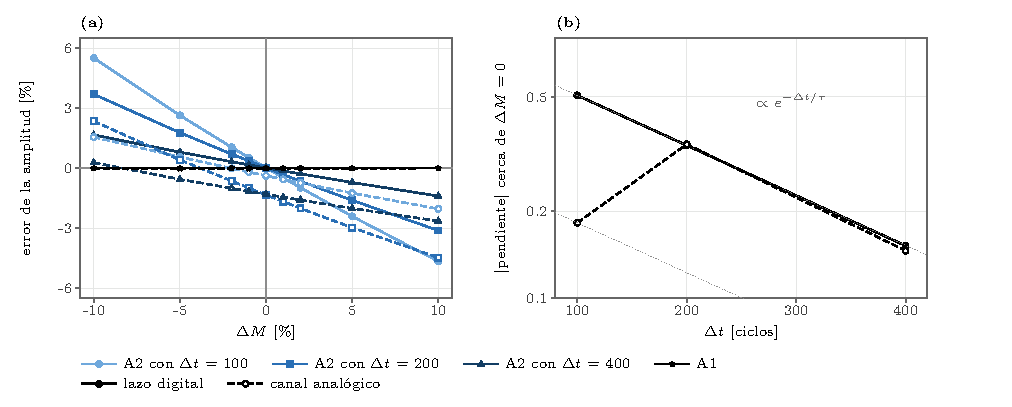
\includegraphics{cap9_meritos_polo_cero}
\caption[Ajuste del polo-cero del trapecio en el lazo digital]{%
Ajuste del polo-cero del trapecio en el lazo digital: pares de 4000 y 2400~ADU
con $\tau = 250$ muestras, separados $\Delta t = 100$, 200 y 400 ciclos, 1000
pares por punto, disparo por polo-cero y la $M$ del trapecio corrida $\Delta M$
entre $-10$ y $+\qty{10}{\percent}$ de la del generador. (a) El error de la
amplitud de $A_2$; (b) la pendiente cerca de $\Delta M = 0$ baja como
$e^{-\Delta t/\tau}$, como la cola de $A_1$ debajo de
$A_2$.\label{f:res-polo-cero}}
\end{figure}

\subsection{Medición de deriva del canal analógico}
\label{S:res-deriva}

Para medir la deriva del canal analógico, alternamos líneas de 1500 y 4000~ADU
cada 3000 ciclos, sin apilamiento, y medimos un punto por minuto durante
\qty{2}{\hour}, con 83\,332 pulsos por punto. En cada punto leímos la
temperatura del Zynq (XADC). Con las dos líneas separamos la deriva en \emph{offset} y
ganancia.

Los resultados se presentan en la Fig.~\ref{f:res-deriva}: en \qty{2}{\hour} la
ganancia recorre 210~ppm, con una pendiente de $-40$~ppm/h. Las líneas recorren
0.8~ADU (la de 1500) y 1.1~ADU (la de 4000), y el \emph{offset} 0.6~ADU. De un minuto
al siguiente las líneas saltan unas 0.12~ADU, 15 veces el error estadístico de
cada punto (0.008~ADU). La temperatura fue de 41.8 a \qty{42.7}{\degreeCelsius},
salvo el primer punto, a \qty{43.2}{\degreeCelsius}. Contra ella la ganancia da
$-144$~ppm/\unit{\degreeCelsius}, con $r = -0.65$. Con un rango de
\qty{1}{\degreeCelsius}, haría falta variar la temperatura a propósito para
separar la temperatura del tiempo.

\begin{figure}[H]
\centering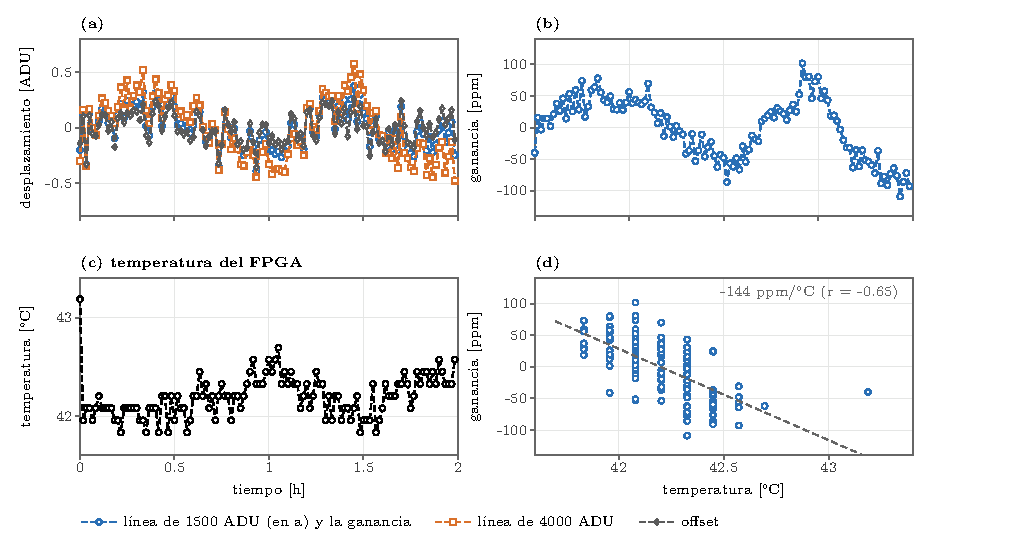
\includegraphics{cap9_meritos_deriva}
\caption[Deriva del canal analógico en 2 h]{%
Deriva del canal analógico en \qty{2}{\hour}: líneas de 1500 y 4000~ADU
alternadas cada 3000 ciclos, 83\,332 pulsos por punto, un punto por minuto, y la
temperatura del Zynq (XADC).\label{f:res-deriva}}
\end{figure}

%==============================================================================
\section{\emph{Throughput} para el osciloscopio}
\label{S:res-throughput-osc}

Como el cambio principal del OSC en este trabajo fue el camino de datos, es la
única propiedad que vamos a describir para este módulo.

La velocidad de registro de eventos se compone de varias operaciones: (1) el
ciclo de lectura de un evento, (2) la agrupación de eventos en un archivo y (3)
la escritura del archivo. La (1) está dada por el HW y la librería de SW, la (2)
únicamente por el SW y la (3) por la capacidad de salida de datos, que puede ser
escritura a la SD o de red. Estas diferencias se presentan en el
Cap.~\ref{C:sw}. En la Fig.~\ref{f:res-throughput} se comparan los siguientes
caminos del \codigo{event\_ring}, que nombramos por el destino de los eventos:
\begin{itemize}
\item DDR: la escritura a DDR.
\item Lector del ring: el lector de C del ring corrido sin guardado en memoria
  secundaria (Sec.~\ref{S:sw-bench-libmca}).
\item SD: el OSC a la SD de la placa por el SW en formato \ruta{.npz}, presentado
  en la Sec.~\ref{S:sw-guardado}.
\item Red: el OSC a la PC por la red.
\end{itemize}
A estos les
sumamos el camino original del osciloscopio, la lectura de la BRAM, con dos
lectores: el lazo de C de \codigo{libmca} y el original, librp desde Python.
Como referencia ponemos el MCA, que no guarda muestras sino que acumula el
espectro en la FPGA.

Llamamos \textbf{techo} de una etapa a la tasa máxima de eventos que puede
sostener cuando la entrada le sobra, es decir, lo que pasa por ella cuando está
saturada. Mientras la entrada está por debajo del techo, la etapa entrega todo
lo que recibe; por encima, entrega su techo y el resto de los eventos se pierde.
Cada etapa tiene el suyo: el de la captura lo fija el HW, el del lector el SW y
el de la red y la SD su ancho de banda.

El techo de la captura sale de su tiempo muerto. Al aceptar un \emph{trigger},
la captura saca la ventana a un canal por ciclo y mientras tanto los
\emph{triggers} nuevos se pierden. Con 2 canales y $S$ = pre + post muestras,
dos eventos tienen que estar separados al menos $2S+3$ ciclos
(Sec.~\ref{S:osc-window-capture}). Con $S=32$ son 67 ciclos de
\qty{8}{\nano\second}, \qty{536}{\nano\second}, y el techo es
$1/\qty{536}{\nano\second}$ $\approx$ 1.87~M/s; con $S=1024$ son 2051 ciclos y el
techo baja a 61~k/s. Con arribos de Poisson la captura se comporta como un
tiempo muerto no paralizable, $m = n/(1+n\tau)$: con $n=3$~M/s y
$\tau=\qty{536}{\nano\second}$ da 1.15~M/s, que es lo que medimos en la DDR.

Las líneas punteadas son los techos. En (a), \codigo{red} y \codigo{SD} son los
techos de cada destino medidos con el ring lleno. En (b), \codigo{captura sola}
es el techo de la captura por su tiempo muerto de $2S+3$ ciclos,
\codigo{TCP solo} el techo por la velocidad de conexión TCP medida con la placa
utilizada (50~MB/s) y \codigo{MCA a 3 M/s} es la tasa
con la que nos comparamos. La recta \codigo{salida = entrada} es la medición
ideal.

\begin{figure}[H]
\centering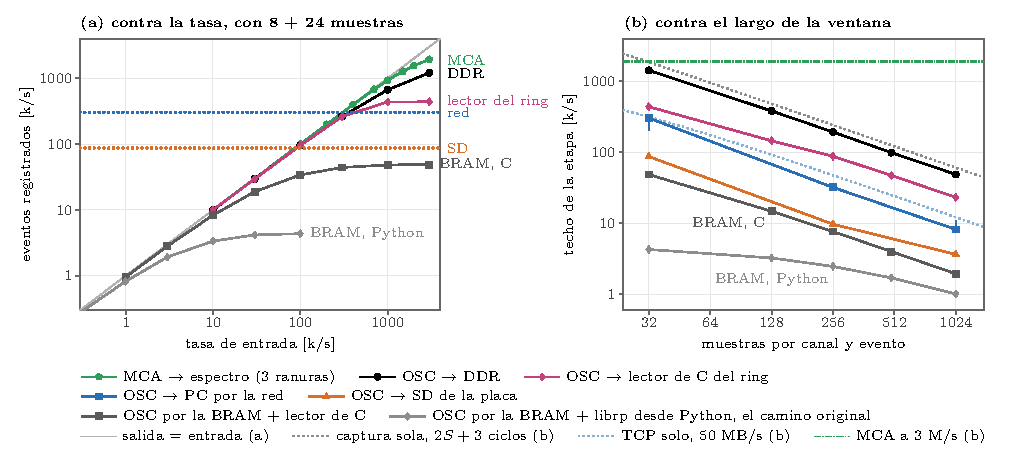
\includegraphics{cap9_throughput_caminos}
\caption[Eventos registrados por segundo en los dos caminos de datos]{%
Eventos registrados por segundo en los dos caminos de datos, medidos en la placa
con generación interna: el MCA, que acumula el espectro en la FPGA, y el
osciloscopio, por el \codigo{event\_ring} o por la BRAM. (a) Tasas
medidas contra las de entrada, con ventanas de 8 + 24 muestras. (b) Techo de
cada etapa contra el largo de la ventana.\label{f:res-throughput}}
\end{figure}

En la Fig.~\ref{f:res-throughput}.a vemos cómo cada etapa recorta la capacidad
de adquisición. Todos los caminos siguen la recta ideal mientras la entrada está
por debajo de su techo y después se aplanan. A 3~M/s de entrada el MCA
registra 1.9~M/s, la captura pone 1.2~M/s en la DDR, el lector
de C del ring lee todo hasta 300~k/s de entrada y se queda en
439~k/s, a la PC por la red llegan 0.3~M/s y a la SD
87~k/s. Cada etapa sostiene lo que le pasa la anterior hasta su propio
techo, así que el camino completo queda fijado por la etapa más lenta. Esto
viene de que tenemos mayor \emph{throughput} para escribir memoria primaria que
secundaria: la DDR acepta lo que captura el HW, mientras que la SD, limitada por
el bus del controlador del Zynq, es la etapa más lenta, y la red queda en el
medio.

La velocidad de adquisición tiene como techo fijo el sistema presentado en HW,
pero ese techo no es el que limita: con ventanas cortas la captura pasa
1.4~M/s y lo que se guarda de forma persistente es entre 5 y 16 veces
menos. En la Fig.~\ref{f:res-throughput}.b vemos que al alargar la ventana
todos los techos bajan. La captura pierde por su tiempo muerto, el lector de C
queda un poco abajo y la red y la SD bajan como su ancho de banda sobre los
bytes por evento ($32+4S$): con 1024 muestras la DDR pasa 49~k/s, el
lector 23~k/s, la red 8.2~k/s y la SD 3.7~k/s. Para el MCA
el largo de la ventana no importa, porque no guarda muestras: este es el motivo
por el que, a igual tasa de entrada, el MCA siempre registra más eventos que el
osciloscopio.

La mejora presente por el osciloscopio se presenta en la comparación con el
camino original por la BRAM, que se lee palabra a palabra por el bus. Con
ventanas de 32 muestras, librp desde Python llega a 4.4~k/s y el lector
de C de la BRAM a 49~k/s, mientras que el lector de C del ring lee
439~k/s: \textbf{100 veces el camino original} y 9 veces el mismo lector
sobre la BRAM. Aún guardando los eventos, por la red llegan 0.3~M/s, unas
70 veces el camino original sin guardar. Con 1024 muestras la diferencia se
achica, porque domina el volumen de datos: el lector del ring pasa
23~k/s contra 1.0~k/s de Python y 2.0~k/s del lector de C
sobre la BRAM.

%%% Local Variables:
%%% mode: latex
%%% TeX-master: "template"
%%% End:
       % Resultados de mérito
% Origen: Secciones/PI - Implementacion OSC.md
% El "Apéndice" de la nota va en apend6.tex (Detalles del osciloscopio).
\chapter{Implementación del OSC}
\label{C:osc}

% Figuras de ESTE capítulo + las compartidas. Siempre al principio del archivo.
\graphicspath{{figs/cap8/}{figs/comunes/}}

\begin{destacado}
En este capítulo se describe (1) las funcionalidades que provee el módulo
osciloscopio empleado, (2) el módulo base de Pitaya, con una descripción
detallada del mecanismo de transferencia de datos al PS, sus limitaciones y el
método de utilización de este módulo desde el PS, y (3) una mejora implementada
en el mecanismo de transferencia y su método de utilización desde el PS. Las
figuras de mérito y comparaciones con el sistema original se presentan en la
Sec.~\ref{S:res-throughput-osc}.
\end{destacado}

%==============================================================================
\section{Función del osciloscopio}
\label{S:osc-funcion}

Su nombre deriva de su funcionamiento principal, que es exactamente igual al de
un osciloscopio. El mismo guarda en un buffer interno una \textbf{traza} de la
señal a su entrada. Esta traza consiste en medidas previas y posteriores al
disparador. Este tipo de funcionalidad es típica de un sistema de HW
programable, debido a que es de las mejores formas de debug de un datapath.
Otros puntos importantes de funcionalidad consisten en:
\begin{itemize}
  \item Largo de traza: en la versión base es un buffer circular fijo de
    $2^\text{RSZ}$ muestras por canal (16384 en el diseño original de Pitaya,
    8192 en este proyecto), del que se configura el largo post-trigger; en la
    versión con anillo de eventos (Sec.~\ref{S:osc-anillo-eventos}) la ventana
    \codigo{pre+post} es configurable hasta 1024 muestras (con \codigo{pre}
    $\leq$ 1023), y por defecto vale 32 (\codigo{pre=8}, \codigo{post=24}).
  \item Mediciones a tiempo de clock de sistema o con un diezmado programable
    (desde 1 hasta 65536).
  \item Disparo por una señal de evento (trigger).
\end{itemize}
Como tenemos toda la información del pulso, no consideramos necesario realizar
un procesamiento en HW de seguimiento de línea de base o compensación de la
misma.

\subsection{Caminos de datos}
\label{S:osc-caminos}

La versión original del osciloscopio proveniente de Pitaya implementa
\textbf{dos metodologías de acceso}. Esto puede comprobarse en la
Fig.~\ref{f:osc-panorama-pitaya}, en la que se presentan dos interfaces AXI: la
primera interactúa con AXI\_GP0 mediante el bus interno del sistema
(\codigo{sys\_bus}), mientras que la segunda escribe en la DDR por los puertos
AXI\_HP0 y AXI\_HP1 (mediante dos bridges, ver la
Sec.~\ref{S:top-vista-general}). Esta interfaz utiliza un esquema de volcado de
datos del tipo \emph{fire and forget} hacia una región de memoria DDR; el
problema de este esquema es que no nos dice nada de la segmentación de los
eventos ni de la consistencia en la lectura de los datos. Estos detalles se
presentan en la Sec.~\ref{S:osc-anillo-eventos}.

Mientras que el bus custom utiliza un handshake completo para leer/escribir
secciones de 32 bits (ver la Sec.~\ref{S:intro-hw-bus-custom}). En la
Sec.~\ref{S:osc-flujo-basico} presentamos los detalles de utilización de esta
modalidad.

\subsection{Vista general del osciloscopio base}
\label{S:osc-vista-general}

Un esquema del funcionamiento del mismo se encuentra en la
Fig.~\ref{f:osc-panorama-pitaya}. Vemos dos regiones: \textbf{una sección
compartida} por todos los canales, representada por bloques en gris, y
\textbf{una cadena de adquisición por stream de datos}. A esta última sección la
subdividimos en otras 4; si hacemos una descripción breve individual por módulo
obtenemos:
\begin{itemize}
  \item \textbf{Cadena de acondicionamiento} (bloques azul claro):
  \begin{itemize}
    \item \codigo{rp\_scope\_calib}: calibración de offset y ganancia,
      $y = \mathrm{sat}\big((x + \text{offset}) \cdot \text{gain}\big)$, con
      saturación al rango de la muestra.
    \item \codigo{osc\_filter}: es un ecualizador IIR que tiene como objetivo
      compensar la respuesta en frecuencia del \emph{front-end} analógico
      (coeficientes \codigo{aa/bb/kk/pp} por canal). Estos son los
      coeficientes comentados en la sección de calibración de Pitaya
      (Sec.~\ref{S:hw-calibracion}).
    \item \codigo{rp\_decim}: reduce la tasa de muestreo por un factor de 1 a
      65536, quedándose con una muestra de cada N o promediándolas
      (\codigo{AVG\_EN}). Llamamos a la unidad de tiempo reducida \emph{tick} y
      no \emph{clock}, para no confundirnos con el reloj del sistema.
    \item \codigo{rp\_delay}: como la salida del trigger está desfasada de los
      datos, este módulo lo compensa: 1 ciclo para los triggers por nivel de
      los canales y 2 para el externo y el del ASG.
  \end{itemize}
  \item \textbf{Cadena de triggering} (bloques amarillos): se calcula en
    paralelo a la cadena de acondicionamiento.
  \begin{itemize}
    \item \codigo{rp\_adc\_trig}: utiliza un disparador con histéresis de tipo
      Schmitt sobre el stream \emph{sin retrasar} del diezmador. Emite un pulso
      de un ciclo en cada flanco de subida (\codigo{trig\_p}) y de bajada
      (\codigo{trig\_n}).
    \item \codigo{rp\_trig\_src}: elige una fuente entre los flancos de los
      canales, el trigger externo, el ASG y el de software (código de 4 bits).
  \end{itemize}
  \item \textbf{Manejo de captura}:
  \begin{itemize}
    \item \codigo{rp\_bram\_sm}: implementa la FSM de armado, post-trigger y
      congelado del buffer, sobre la que el PS hace los 3 pasos de la sección
      siguiente. Se explica en detalle en la Sec.~\ref{S:ap-osc-fsm-bram} del
      Apéndice.
  \end{itemize}
  \item \textbf{Manejo de transacciones}:
  \begin{itemize}
    \item \codigo{rp\_acq\_bram}: buffer circular de $2^\text{RSZ}$ muestras de
      14 bits (RSZ = 14 en el original, 13 en este proyecto). Se lee mediante
      el \codigo{sys\_bus}, una muestra por transacción.
    \item \codigo{rp\_axi\_sm}: camino paralelo que hace uso de \emph{direct
      memory access} (DMA). Se describe en detalle en la
      Sec.~\ref{S:osc-anillo-eventos}.
  \end{itemize}
\end{itemize}

\begin{figure}[H]
\centering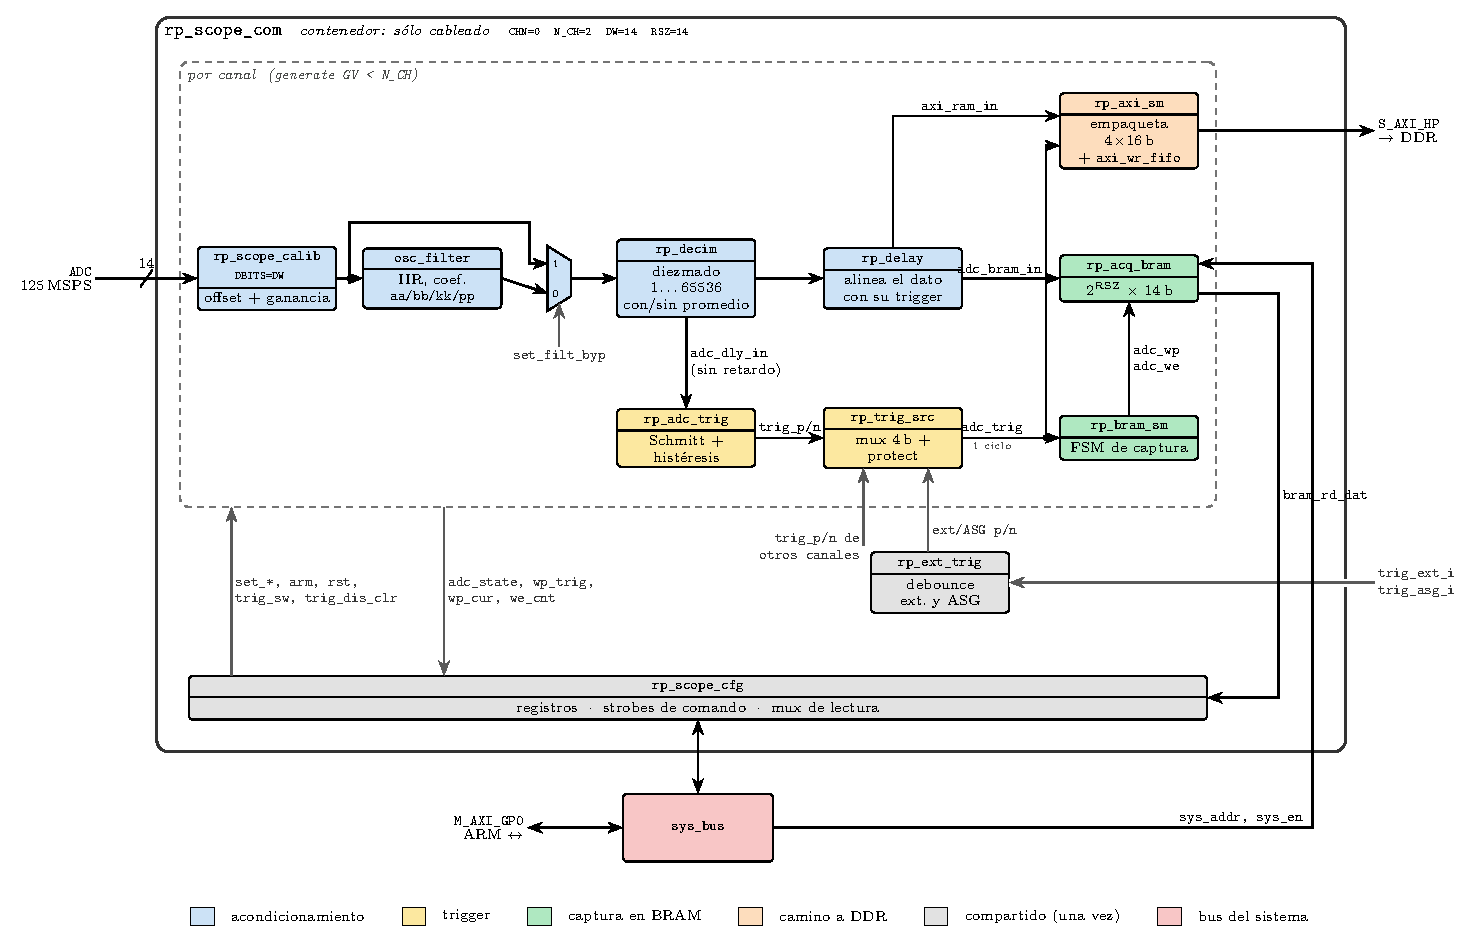
\includegraphics{cap8_panorama_scope_pitaya}
\caption[Módulo OSC original de Pitaya]{%
Módulo OSC original de Pitaya. Contiene una cadena de preprocesamiento (azul),
sección de triggering interno (amarillo) y externo (módulo
\codigo{rp\_ext\_trig} en gris), submódulo de configuración (en gris), lógica de
captura de datos y manejo de transacciones por bus custom (verde) y camino de
datos por HP (\codigo{rp\_axi\_sm} en naranja claro).\label{f:osc-panorama-pitaya}}
\end{figure}

Mientras que si desarrollamos los \textbf{bloques compartidos} encontramos los
dos siguientes:
\begin{itemize}
  \item \codigo{rp\_ext\_trig}: es un \emph{debouncer} de longitud configurable
    para el trigger externo y del ASG.
  \item \codigo{rp\_scope\_cfg}: guarda la configuración y maneja los comandos
    desde SW a la FSM. Multiplexa hacia \codigo{sys\_bus} la lectura del estado
    y de la BRAM.
\end{itemize}

\subsection{Flujo de funcionamiento básico}
\label{S:osc-flujo-basico}

El proyecto base de Pitaya ya contaba con un módulo capaz de implementar una
versión básica de esta funcionalidad mediante el bus custom. En la
Fig.~\ref{f:osc-secuencia-basica} se presentan los pasos para realizar una
captura: primeramente tenemos que realizar todas las configuraciones
necesarias, mientras que por traza capturada tenemos que seguir los siguientes
pasos:
\begin{enumerate}
  \item \textbf{Armado} (\emph{arm}): es mandar el comando de armado
    \codigo{CMD\_ARM}, que se realiza escribiendo un 1 a este registro. Indica al
    módulo que terminó de trabajar con su buffer interno y que es capaz de
    sobreescribirlo.
  \item \textbf{Chequeo de finalización de captura} (congelamiento): se lee la
    variable \codigo{ADC\_STATE} hasta que la vemos en alto. Representa que el
    módulo terminó de adquirir la traza deseada y se encuentra disponible para
    leer.
  \item \textbf{Lectura}: el buffer interno se encuentra congelado; en este
    estado se realizan las transacciones de lectura necesarias para extraer
\end{enumerate}

\begin{figure}[H]
\centering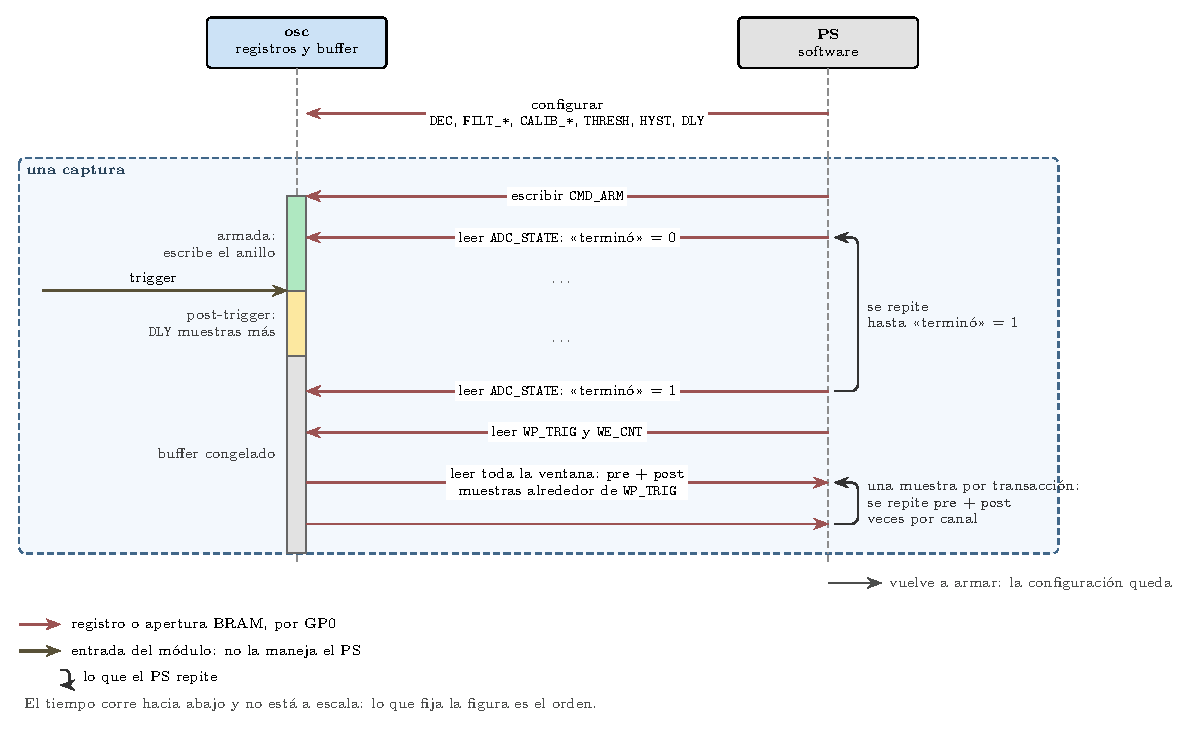
\includegraphics{cap8_secuencia_osc}
\caption[Secuencia de una captura del OSC básico]{%
Secuencia de una captura del OSC básico vista desde el PS, en modo single-shot
(\codigo{keep = 0}). El PS arma, sondea \codigo{ADC\_STATE} hasta que el buffer
queda congelado y recién entonces lee los punteros y la traza por el bus.
Mientras el PS lee, la captura está detenida.\label{f:osc-secuencia-basica}}
\end{figure}

Un sistema de adquisición ``continua'' realiza un loop en estas tres fases. El
sistema también aporta un registro de configuración \codigo{keep} (modo
continuo): con \codigo{keep=1} el buffer nunca se congela, y después de cada
post-trigger la escritura sigue y la FSM queda esperando el próximo trigger. Se
detiene escribiendo \codigo{keep=0} y esperando que el sistema se congele.

Para que no tengamos sobreescritura del buffer, tenemos que estar seguros de que
no tenemos triggers mientras realizamos la lectura. Esto puede ser el caso si
nosotros lanzamos el trigger de forma externa o por SW. En el caso de no tener
control sobre el trigger, el modo \codigo{keep} no es deseable, debido a que
podemos tener \emph{tearing}: bajo este efecto, una lectura del buffer puede
resultar de una cantidad arbitraria de capturas.

En la Fig.~\ref{f:osc-secuencia-basica} las flechas PS$\rightarrow$PL son
escrituras (la configuración y el \codigo{arm}) y las PL$\rightarrow$PS son
lecturas (el estado, y los punteros y el buffer una vez congelado). Todas las
transacciones se realizan mediante el ``handshake completo'' explicado en la
Sec.~\ref{S:intro-hw-transferencia}.

El ciclo completo (armar, esperar el congelado, leer la ventana y volver a
armar) tarda $\tau = \qty{252.7}{\micro\second}$ medido en placa, y lo domina
la lectura de la ventana de a una muestra por transacción
(\qty{45.6}{\micro\second} por canal). Mientras tanto el hardware no puede
capturar: es una cola de capacidad $K = 1$, y los eventos que llegan en ese
lapso no quedan registrados en ningún contador. La
Sec.~\ref{S:osc-anillo-eventos} presenta cómo se elimina esa espera.

%==============================================================================
\section{Cambios realizados en la versión básica del proyecto}
\label{S:osc-cambios}

Las diferencias principales fueron dos. Primeramente, \textbf{aislamos la cadena
de acondicionamiento y exportamos la cadena de triggering} a su propio módulo
\textbf{multitrigger}, explicado en el Cap.~\ref{C:multitrigger}. Por otro lado,
volcamos como salidas los pasos intermedios del DSP mediante la utilización de
tres seleccionadores llamados \textbf{mca}, \textbf{mtrg} y \textbf{osc}; estos
últimos pueden verse en la Fig.~\ref{f:osc-panorama-scope-mt} representados en
gris. En la Sec.~\ref{S:top-datapath} se presentan estas decisiones en más
detalle.

\begin{figure}[H]
\centering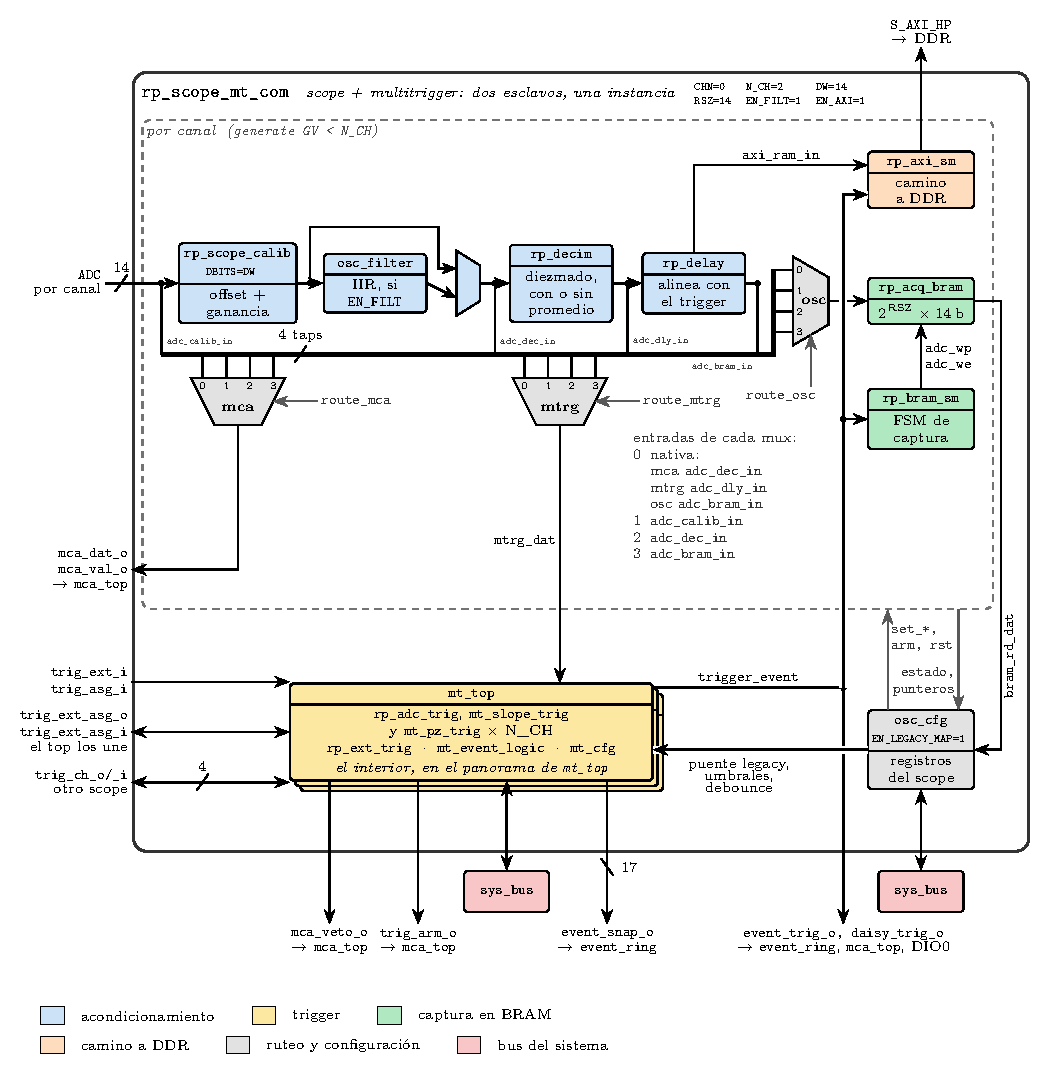
\includegraphics{cap8_panorama_scope_mt}
\caption[Módulo del scope utilizado en este proyecto]{%
Módulo del scope utilizado en este proyecto (\codigo{rp\_scope\_mt\_com}). La
cadena de triggering pasa a \codigo{mt\_top}, plegado (con sombra), y tres
\codigo{dsp\_tap\_mux} (en gris) eligen de qué nodo del DSP toma su muestra cada
consumidor: MCA, multitrigger y OSC. \codigo{trigger\_event} dispara a la vez la
captura de todos los canales, y todo corre en
\codigo{adc\_clk}.\label{f:osc-panorama-scope-mt}}
\end{figure}

%==============================================================================
\section{Versión anillo de eventos}
\label{S:osc-anillo-eventos}

El osciloscopio original de Red Pitaya cuenta con un camino de datos paralelo,
implementado en \codigo{rp\_axi\_sm} (no confundir con la
\codigo{rp\_bram\_sm}). En la Fig.~\ref{f:osc-deep-memory} se presenta el
mecanismo: después de un armado, las muestras se escriben de forma continua en
la memoria DDR del PS mediante la interfaz HP (en este camino el PL es master),
igual que en la BRAM, y tras el post-trigger la escritura se congela y se
actualizan los registros internos del módulo dentro del PL. Para averiguar en
qué sección de los 2~MB se encuentra el pulso, se tiene que realizar una
transacción de lectura al PL acerca de estas variables.

\begin{figure}[H]
\centering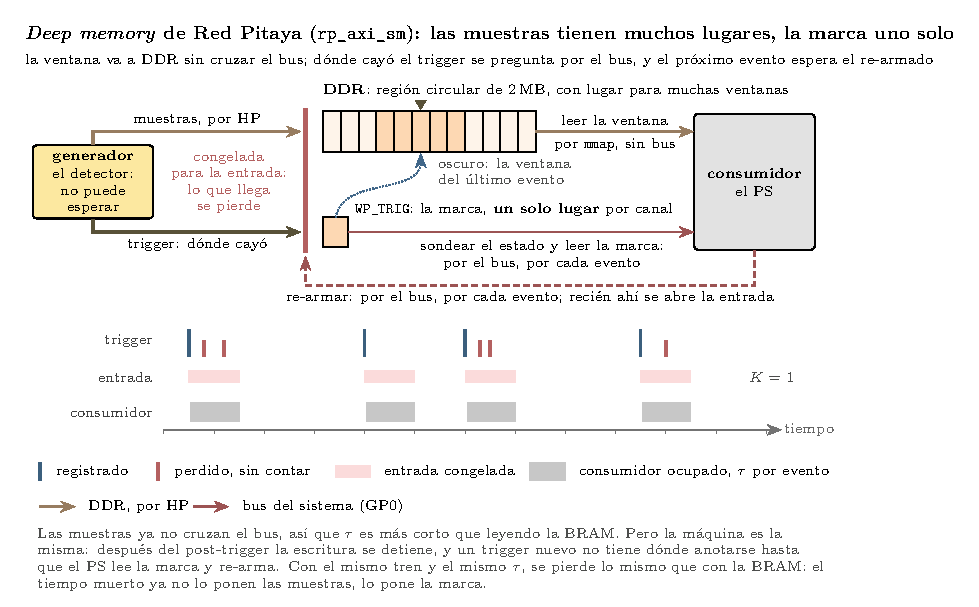
\includegraphics{cap8_deep_memory}
\caption[Esquema del \emph{deep memory} de Pitaya]{%
Esquema del \emph{deep memory} de Pitaya (\codigo{rp\_axi\_sm}) como generador,
buffer y consumidor. Las muestras van a DDR por HP, donde entran muchas
ventanas, pero dónde cayó el trigger se anota en un único registro
(\codigo{WP\_TRIG}). La entrada queda congelada hasta que el PS lo lee por el bus
y re-arma: se comporta como un buffer de $K = 1$. Es un esquema, no una
medición.\label{f:osc-deep-memory}}
\end{figure}

Esto parecería deseable, porque contamos con una región de memoria que puede
contener hasta $K$ eventos dentro de la misma, acercándonos a los requerimientos
de un sistema insensible a la latencia presentado en la
Sec.~\ref{S:intro-hw-latencia}. La gran diferencia entre este sistema y el
presentado es que el lector puede congelar el sistema aun teniendo toda la
memoria libre dentro del mismo. Este hecho hace que se comporte como uno con
$K=1$, debido a que la razón de existencia de este módulo es independizar ambos
extremos de la cola (o que queden únicamente asociados por la capacidad máxima
de la cola). Aun así, este sistema presenta mejoras con respecto al previo: no
tenemos que realizar un acceso palabra a palabra (32 bits) de la traza del
osciloscopio, así que reducimos el tiempo muerto por la transferencia de los
datos. Este tiempo es lineal con el largo de la transferencia, así que puede
ser muy útil si queremos obtener trazas considerablemente largas.

Este bloqueo se debe a que la presencia de un nuevo evento puede reescribir
cualquiera de los valores previos; esto \textbf{es considerar que la totalidad
del resto del buffer no se puede sobreescribir}, y no es necesariamente verdad.
Cada evento puede tomar una región de memoria dedicada en el buffer, de largo y
posición fija en DDR; esta región tiene en cuenta la segmentación del pulso en
hardware. La comparación entre el buffer segmentado y el original se presenta en
la Fig.~\ref{f:osc-ring-vs-buffer}. A cada región para un pulso la llamamos
casillero (\emph{slot}), y \textbf{contiene las variables de control que antes
transferíamos por GP0}. En la Fig.~\ref{f:osc-ring-vs-buffer}(b) se presenta su
estructura interna, que consiste en las regiones:
\begin{itemize}
  \item \textbf{Header} (cabecera): contiene los valores de metadata del
    evento; incluye el timestamp, la cantidad de canales, la cantidad de
    muestras, el número en la secuencia y el snapshot de trigger (qué trigger lo
    lanzó).
  \item \textbf{Datos+relleno}: contiene las muestras de la ventana más una
    región inválida para normalizar el ancho de los slots.
  \item \textbf{Footer}: es la marca de \emph{commit}: indica que el slot está
    completo. Si el slot se puede volver a escribir no lo dice el footer sino
    los créditos (\codigo{RD\_SLOT}).
\end{itemize}

\begin{figure}[H]
\centering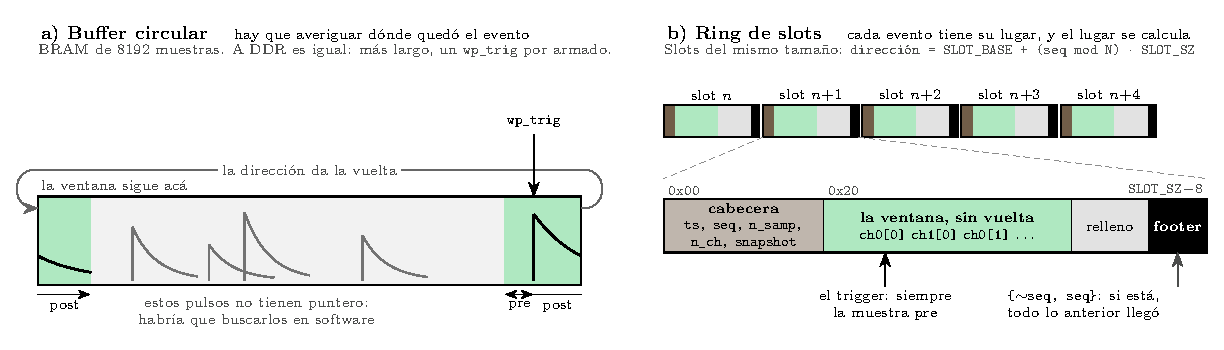
\includegraphics{cap8_ring_vs_buffer}
\caption[Dónde queda un evento en DDR: buffer circular y anillo de slots]{%
Dónde queda un evento en DDR. (a) Buffer circular: las muestras se escriben
corridas, y sólo el último evento tiene puntero (\codigo{wp\_trig}); los
anteriores habría que buscarlos en software. (b) Anillo de slots: cada evento
ocupa un slot de largo fijo, con cabecera, muestras, relleno y el footer
\codigo{\{\textasciitilde seq, seq\}}, y su dirección se calcula como
\codigo{SLOT\_BASE + (seq mod N)$\cdot$SLOT\_SZ}.\label{f:osc-ring-vs-buffer}}
\end{figure}

Esta implementación libera ancho de banda en el canal (no estamos transfiriendo)
y, mucho más importante, podemos subdividir la lectura del mismo en hasta la
cantidad de slots que deseemos. Este esquema de comunicaciones se suele
describir como \emph{descriptor ring}~\cite{Virtio12,Corbet2005}. A
continuación describimos cómo funciona la sección de control, vista desde el PS.

\subsection{Funcionamiento del footer}
\label{S:osc-footer}

Es una \textbf{marca de \emph{commit} al final del slot}: si no tiene el valor
esperado, el PS no lee el resto. Es el mecanismo habitual cuando un mensaje es
largo o su latencia es desconocida: se escribe el cuerpo y, al final, una marca
que confirma que todo lo anterior ya llegó. Como el PL escribe el slot en orden
de dirección, ver el footer con el \codigo{seq} esperado garantiza que la
cabecera y las muestras ya están en la DDR. El PS tampoco tiene que confirmar
cada evento: devuelve \textbf{créditos} publicando \codigo{RD\_SLOT} una vez por
lote, y el PL escribe de forma ininterrumpida mientras le queden créditos.

\subsection{Metodología de utilización del anillo}
\label{S:osc-uso-anillo}

En la Fig.~\ref{f:osc-secuencia-ring} se presentan las transacciones. Se habla
de lote porque se aprovecha que los elementos ya están en DDR para agruparlos en
regiones contiguas y así realizar movimientos de datos más eficientes. Para que
esto funcione de forma correcta tenemos que configurar los parámetros de la
región de memoria; estos sólo se latchean con la adquisición parada, y
escribirlos corriendo se ignora y levanta la flag \codigo{err\_cfg}. Incluyen:
\begin{enumerate}
  \item Tamaño \codigo{RING\_SZ} y posición de la región de DDR volátil (este
    tipo de acceso a memoria debe configurarse en el OS; el anillo usa la región
    de 32~MB en \codigo{0x0A00\_0000} que el proyecto de Pitaya reserva para el
    analizador lógico, y no la de 2~MB del \emph{deep memory}).
  \item Tamaño del \codigo{SLOT\_SHIFT}.
  \item Cantidad de slots, que no se escribe: el módulo la deriva como
    \codigo{N\_SLOTS = RING\_SZ \textgreater\textgreater{} SLOT\_SHIFT}. Todos
    deben entrar en la región DDR asignada.
  \item Tamaño de PRE y POST trigger de la ventana. La cabecera, la ventana y el
    footer deben entrar en un slot de $2^\text{SLOT\_SHIFT}$ bytes.
\end{enumerate}
Antes de escribir la geometría, el PS para el anillo, espera que llegue a
\codigo{STOPPED} y escribe \codigo{CTRL.clr}. Esto vacía el stage, el escritor
y el \codigo{axi\_wr\_fifo}, pone en cero \codigo{WR\_SLOT}, \codigo{RD\_SLOT},
\codigo{SEQ} y los contadores de descarte, y limpia \codigo{err\_cfg}. Después
el PS \textbf{pone en cero el footer de cada slot}, escribiendo directamente en
la DDR: el slot $k$ de la corrida anterior tiene el mismo \codigo{seq} que
tendrá el de esta, con un footer válido, y sin borrarlo la primera vuelta lo
entregaría como nuevo. Con una barrera de por medio escribe la geometría, la
relee (\codigo{N\_SLOTS}, \codigo{err\_cfg} y \codigo{WR\_SLOT = 0}) y recién
entonces activa el módulo con \codigo{CTRL.run} (ver la
Fig.~\ref{f:osc-fsm-ring}).

Por simplicidad, asociamos un único hilo de ejecución dentro del PS para este
módulo. El código del Cap.~\ref{C:sw} realiza lo siguiente:
\begin{enumerate}
  \item Lee \codigo{WR\_SLOT} por GP0 una vez por lote de eventos, para saber
    cuántos slots hay candidatos.
  \item Valida el footer de cada uno en la DDR. El primero que no está corta el
    bloque, porque \codigo{WR\_SLOT} avanza cuando el FIFO acepta el footer, no
    cuando el footer llega a la DDR.
  \item Pone una barrera de memoria, que ordena los accesos: garantiza que los
    footers se leyeron antes que los datos (ver la
    Sec.~\ref{S:hw-modelo-memoria}). Recién después lee la cabecera y las
    muestras.
  \item Pone otra barrera y publica \codigo{RD\_SLOT} una vez por bloque,
    devolviendo los créditos de todos sus slots.
\end{enumerate}
Con el buffer circular el trabajo era \textbf{por evento}, y la captura queda
congelada mientras el PS lee. Con el ring es \textbf{por lote} y la captura no
se detiene.

\begin{figure}[H]
\centering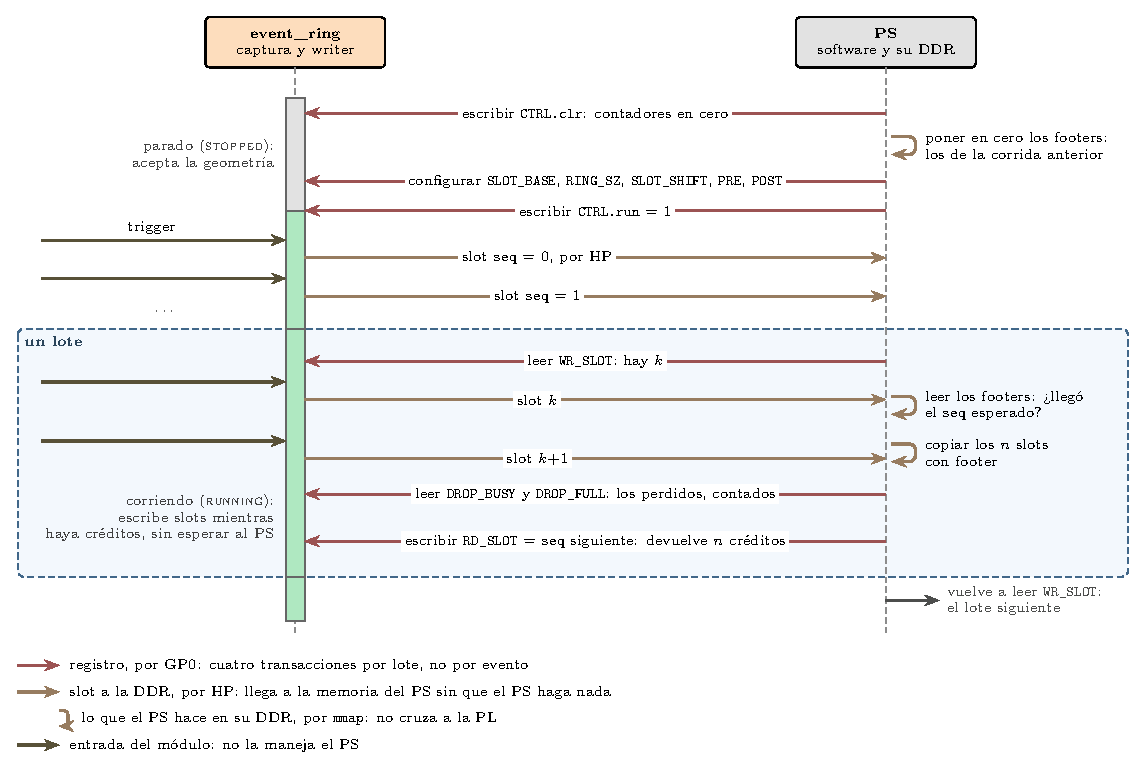
\includegraphics{cap8_secuencia_ring}
\caption[Flujo de utilización del anillo de eventos]{%
Flujo de utilización del anillo de eventos. Tenemos tres fases: (1)
inicialización, (2) arranque y (3) lectura por lote, con el commit dado por el
footer (\codigo{seq}) y el acknowledge por la escritura de
\codigo{RD\_SLOT}.\label{f:osc-secuencia-ring}}
\end{figure}

Si se quisiera, se podría sondear sólo el footer y no leer \codigo{WR\_SLOT}. La
diferencia es que sin \codigo{WR\_SLOT} el lazo no toca el GP0, pero el PS no
sabe cuántos slots hay listos y tiene que leer los footers de a uno hasta dar
con uno que no está. Con \codigo{WR\_SLOT}, una sola lectura por bloque
($\sim$\qty{2.3}{\micro\second}, repartidos entre todos los eventos del bloque)
dice cuántos pedir, y el commit lo sigue dando el footer.

En la siguiente sección mostramos la vista general del módulo que implementa la
comunicación mediante el anillo.

\subsection{Panorama del módulo del anillo}
\label{S:osc-panorama-anillo}

El anillo reemplaza al camino a DDR original: \codigo{rp\_axi\_sm} queda
deshabilitado (\codigo{EN\_AXI = 0}) y en su lugar se usa
\codigo{event\_ring\_top}, con las conexiones de la
Fig.~\ref{f:osc-panorama-scope-ring}. En el bitstream el anillo no está dentro
del scope sino en el TOP, al lado de él, con esas mismas conexiones. Se dejó el
camino original por AXI\_GP0 y la BRAM porque la versión original del módulo
contenía ambos caminos, y por compatibilidad del mapa de registros.

\begin{figure}[H]
\centering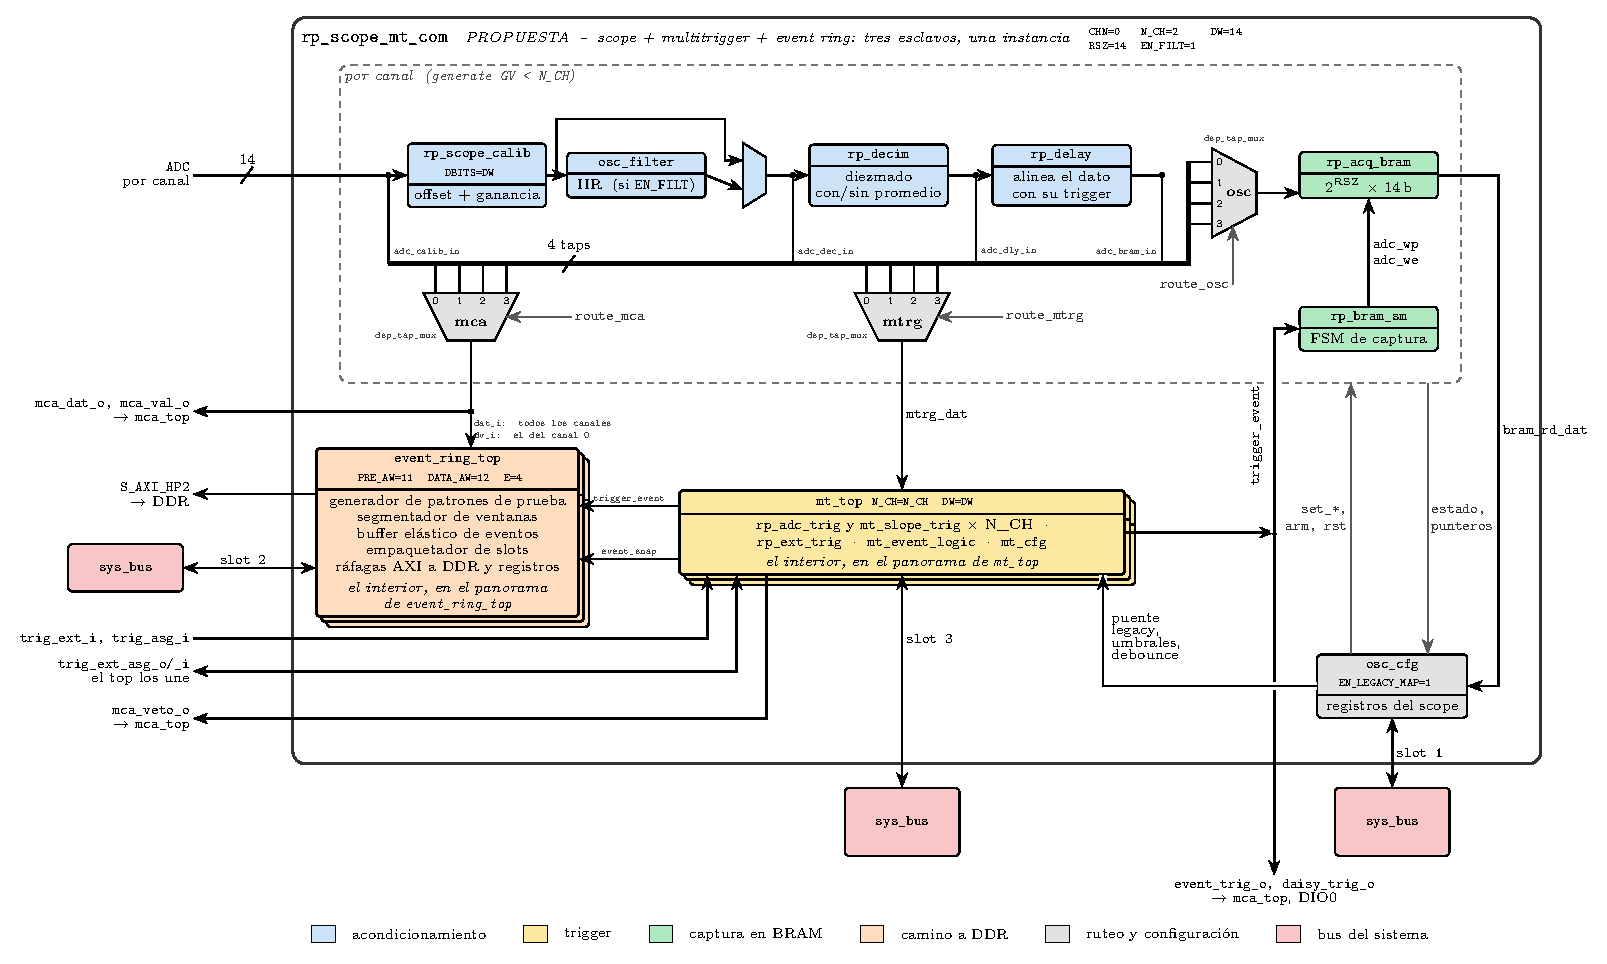
\includegraphics{cap8_panorama_scope_ring}
\caption[Conexión del anillo de eventos con el scope]{%
Conexión del anillo de eventos con el scope. \codigo{event\_ring\_top} toma el
lugar de \codigo{rp\_axi\_sm}, el camino a DDR. La BRAM se mantiene porque es la
que leen \codigo{librp} y la secuencia del OSC básico. Los bloques con sombra
están plegados: su interior está en los panoramas de \codigo{mt\_top} y
\codigo{event\_ring\_top}. En el bitstream el anillo se instancia en el TOP, al
lado del scope, con estas mismas conexiones.\label{f:osc-panorama-scope-ring}}
\end{figure}

%==============================================================================
\section{Funcionamiento del módulo de ring de eventos}
\label{S:osc-ring-funcionamiento}

En la Fig.~\ref{f:osc-freno-descarte} se puede ver la cadena principal del
datapath del módulo de ring de eventos \codigo{event\_ring\_top}, que contiene
los siguientes submódulos:
\begin{itemize}
  \item \codigo{event\_window\_capture}: es el que segmenta las muestras de la
    entrada en las trazas correspondientes a subir al FIFO.
  \item \codigo{event\_stage\_fifo}: es un \textbf{buffer
    elástico}~\cite{Cortadella2006} que guarda todas las fuentes de datos de un
    evento en buffers separados.
  \item \codigo{event\_slot\_writer}: arma la trama de bits que representa un
    slot a partir de los datos de los buffers de la etapa anterior, es decir,
    serializa un evento a un slot del anillo en DDR. Sale por la misma interfaz
    simplificada de Instrumentation Technologies que usaba
    \codigo{rp\_axi\_sm}, para seguir el formato del sistema original.
  \item \codigo{axi\_wr\_fifo}: módulo de paquetizado del proyecto original de
    Pitaya, requerido para pasar a la interfaz HP2, del tipo AXI-Full. A este no
    se lo describirá porque no fue parte de este proyecto; para más información
    se refiere a la documentación oficial de Pitaya~\cite{RedPitayaFPGA}.
\end{itemize}

\begin{figure}[H]
\centering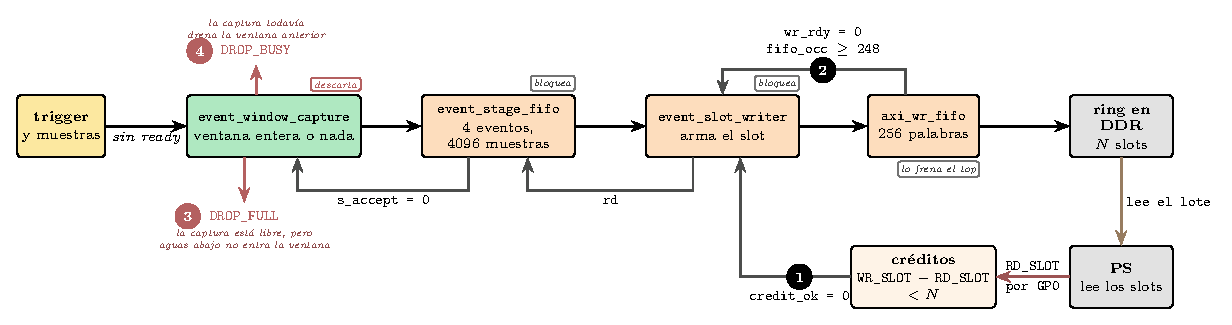
\includegraphics{cap8_ring_freno_descarte}
\caption[Dónde se frena y dónde se descarta en el anillo]{%
Dónde se frena y dónde se descarta en el anillo cuando algo no alcanza. Sólo la
captura descarta, porque el trigger y las muestras le llegan sin
\codigo{ready}: el evento que no puede tomar lo pierde entero y lo cuenta
(flecha roja). El stage y el escritor sólo bloquean, y su contrapresión
(flechas de vuelta) sube hasta la captura sin perder datos. Los números son las
filas de la Tabla~\ref{t:osc-freno-descarte}.\label{f:osc-freno-descarte}}
\end{figure}

Como explicamos en la Sec.~\ref{S:intro-hw-back-pressure}, la cantidad de
eventos perdidos en toda la cadena es igual a la \textbf{suma de eventos
perdidos en cada una de las etapas individuales}, si lo expandimos al sistema
actual.

Si analizamos la composición interna del módulo, además de la cadena principal
(en naranja claro) identificamos las siguientes cinco secciones de lógica
propias del top:
\begin{itemize}
  \item \textbf{Submódulo de configuración}: sección compartida explicada en la
    Sec.~\ref{S:intro-hw-modulo-config}.
  \item \textbf{Timestamp}: contador de 64 bits que avanza con cada
    \codigo{dv}. Vuelve a 0 en \codigo{STOPPED}, así que $t = 0$ es el arranque
    de la corrida. La captura lo copia en la cabecera de cada evento.
  \item \textbf{Créditos}: calcula los slots ocupados en la DDR como
    \codigo{wr\_slot $-$ rd\_slot}, así que funciona aunque los contadores den
    la vuelta. \codigo{credit\_ok = ocupados \textless{} N\_slots}.
    \codigo{rd\_slot} lo publica el PS cuando termina de leer un lote. Sin
    crédito, el writer espera para no pisar un slot que el PS todavía no leyó.
  \item \textbf{Dirección}: indica los valores límite dados los registros de
    configuración internos, stop = \codigo{SLOT\_BASE + RING\_SZ $-$ 8}.
  \item \textbf{Contrapresión}: calcula una ocupación propia del
    \codigo{axi\_wr\_fifo} por el master. Hace falta porque el FIFO del
    proyecto de Pitaya no expone su nivel y \textbf{descarta en silencio si se
    pushea estando lleno}. Si aun así el FIFO desborda, queda un sticky
    \codigo{err\_fifo\_ovf}.
\end{itemize}

\begin{figure}[H]
\centering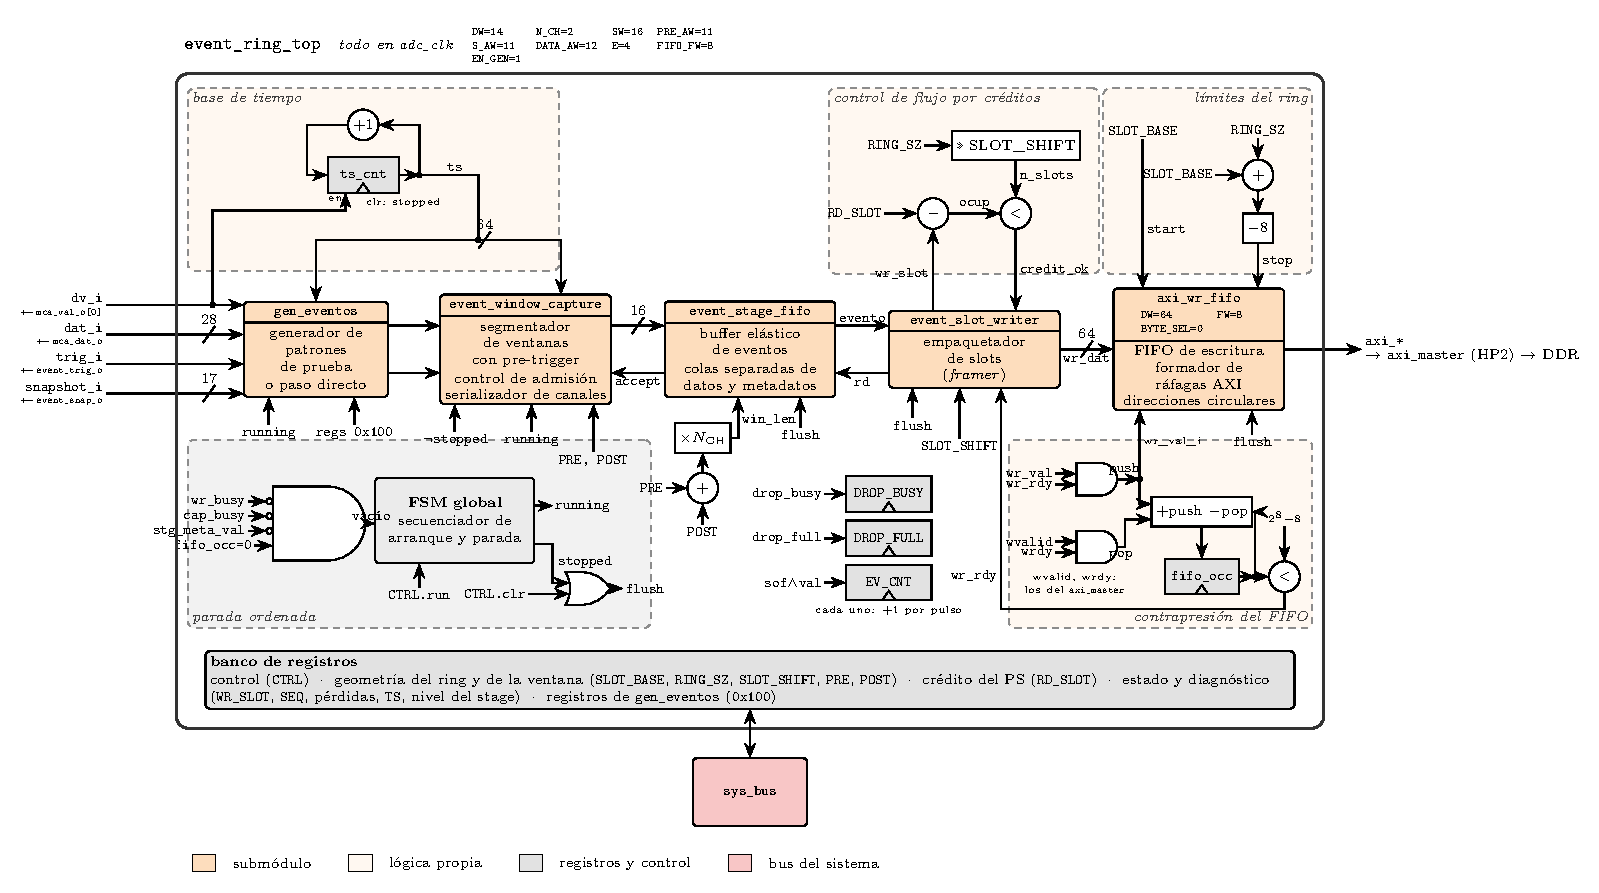
\includegraphics{cap8_panorama_event_ring_top}
\caption[Estructura interna de \codigo{event\_ring\_top}]{%
Estructura interna de \codigo{event\_ring\_top}. Contiene la cadena de la
Fig.~\ref{f:osc-freno-descarte} (en naranja claro) y la lógica propia del top:
configuración, timestamp, créditos, dirección, contrapresión y FSM global. El
PS no lee ningún registro por evento: lee \codigo{WR\_SLOT} y publica
\codigo{RD\_SLOT} una vez por lote, y valida cada slot por su footer en DDR.
\codigo{gen\_eventos} está entre la entrada y la captura; apagado, es un paso
directo.\label{f:osc-panorama-ring-top}}
\end{figure}

Nos quedó por explicar el \textbf{manejo de la FSM}: en la
Fig.~\ref{f:osc-fsm-ring} se puede observar una FSM global de tres estados
(\codigo{STOPPED}, \codigo{RUNNING}, \codigo{DRAINING}). En \codigo{STOPPED} se
vacían el stage, el escritor y el \codigo{axi\_wr\_fifo}, y se ponen en cero
\codigo{wr\_slot}, \codigo{rd\_slot} y el timestamp; es el único estado en que
se acepta la geometría. En \codigo{RUNNING} la captura acepta triggers. Al bajar
\codigo{CTRL.run} pasa a \codigo{DRAINING}: la captura no acepta triggers nuevos
pero termina la ventana en vuelo, y vuelve a \codigo{STOPPED} recién cuando la
captura y el escritor están libres, el stage no tiene eventos y el
\codigo{axi\_wr\_fifo} largó su última palabra. Así una parada nunca deja un
slot sin su footer.

\begin{figure}[H]
\centering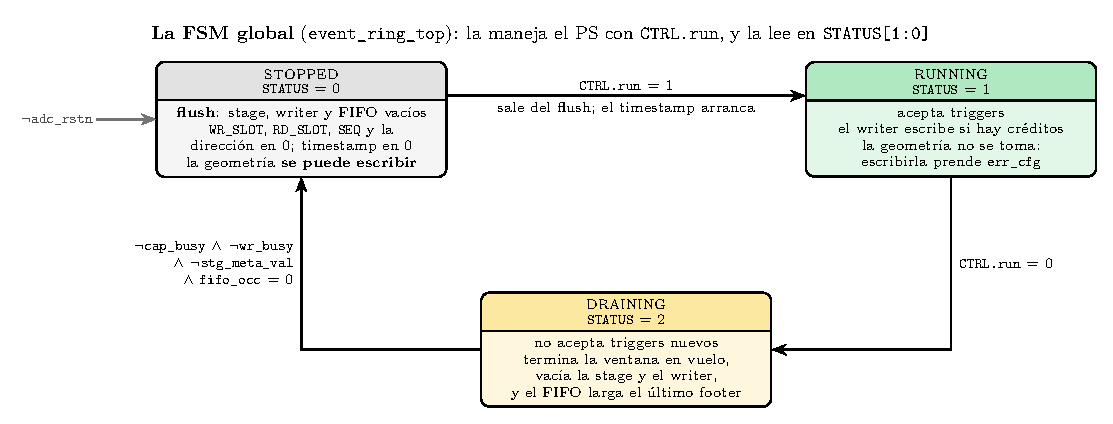
\includegraphics{cap8_fsm_event_ring_top}
\caption[FSM global del anillo de eventos]{%
FSM global del anillo de eventos, que el PS maneja con \codigo{CTRL.run} y lee
en \codigo{STATUS[1:0]}. \codigo{DRAINING} deja terminar la ventana en vuelo y
vacía la cadena antes de volver a \codigo{STOPPED}. Si se para con el anillo
lleno, no termina hasta que el PS devuelve créditos o escribe
\codigo{CTRL.clr}. Llegar a \codigo{STOPPED} pone en cero los contadores de
slot.\label{f:osc-fsm-ring}}
\end{figure}

\subsection{Cálculo de tiempo muerto y contadores presentes}
\label{S:osc-tiempo-muerto}

Recordemos que el tiempo muerto es el tiempo durante el cual el sistema no puede
aceptar un evento nuevo; los eventos que llegan en ese lapso se pierden. En la
Fig.~\ref{f:osc-freno-descarte} se presentan todas las etapas principales del
anillo de eventos implementado. Todas las etapas cuentan con una conexión
trasera con la cual emiten la disponibilidad del módulo a una nueva
transacción; este es un bloqueo controlado del flujo de datos.

Es importante notar que la etapa que toma en cuenta los créditos no es la que
tiene conexión directa con la interfaz AXI, el \codigo{axi\_wr\_fifo}, sino la
penúltima, \codigo{event\_slot\_writer}. Esto se debe a que
\codigo{axi\_wr\_fifo} es un paquetizador: no tiene en cuenta el mecanismo de
transferencia de datos implícito en el módulo (la versión expandida que
referenciamos al final de la Sec.~\ref{S:intro-hw-transferencia}). Si
describimos en más detalle todos estos pasos, nos vamos a encontrar con la
información presentada en la Tabla~\ref{t:osc-freno-descarte}.

\begin{table}[H]
\centering
\caption[Recursos que pueden agotarse en el anillo]{%
Recursos que pueden agotarse en el anillo, la señal que lo indica y qué pasa en
cada caso. Los niveles 1 y 2 \textbf{frenan} al escritor sin perder datos; los 3
y 4 \textbf{descartan} el evento entero en la captura y lo cuentan en
\codigo{DROP\_FULL} y \codigo{DROP\_BUSY}.\label{t:osc-freno-descarte}}
\small
\begin{tabularx}{\textwidth}{|c|>{\raggedright\arraybackslash}p{0.27\textwidth}%
  |l|>{\raggedright\arraybackslash}X|}
\hline \encabezado \textbf{Nivel} & \textbf{Recurso} & \textbf{Señal} &
  \textbf{Qué pasa al agotarse} \\ \hline
1 & slots de DDR & \codigo{credit\_ok} & el writer \textbf{se frena} en
  \codigo{W\_IDLE} \\ \hline
2 & \codigo{axi\_wr\_fifo} & \codigo{wr\_rdy} & el writer \textbf{se frena} a
  mitad de slot \\ \hline
3 & stage (muestras + metadatos) & \codigo{s\_accept} & la captura
  \textbf{descarta entero} $\rightarrow$ \codigo{drop\_full} \\ \hline
4 & la captura misma & \codigo{busy} & trigger durante el drenaje
  $\rightarrow$ \codigo{drop\_busy} \\ \hline
\end{tabularx}
\end{table}

%==============================================================================
\section{Detalles de submódulos}
\label{S:osc-submodulos}

\subsection{Módulo de captura de ventana:
\texorpdfstring{\texttt{event\_window\_capture}}{event\_window\_capture}}
\label{S:osc-window-capture}

Reemplaza el rol de \codigo{rp\_bram\_sm}. Este módulo es común a todos los
slots, y su funcionalidad consiste en que por cada \textbf{trigger se extrae una
ventana de muestras como un AXI-Stream}; la misma incluye \codigo{pre} antes y
\codigo{post} desde el disparo.
\begin{itemize}
  \item Tiene \textbf{una sola memoria}, el pre-buffer: un buffer circular de
    $2^{11}$ palabras que se escribe siempre y del que salen tanto el pre como
    el post. Los metadatos del evento (\codigo{m\_ts}, \codigo{m\_snap},
    \codigo{m\_nsamp}) se guardan en tres registros.
  \item El evento se acepta o se descarta entero; esto se decide en el ciclo del
    trigger, antes de emitir el \emph{start of frame} (SOF).
\end{itemize}

Tenemos una segmentación de las ventanas de captura mediante la utilización de
símbolos que representan el inicio de una ventana, llamado \emph{start of frame}
(SOF), y el final de la ventana, llamado \emph{end of frame} (EOF). La FSM del
sistema se presenta en la Fig.~\ref{f:osc-fsm-window}; lo más importante es que
mueve \textbf{sólo el lado de lectura del pre-buffer} y consta de tres estados.

Con \codigo{run\_i} en 1, cada \codigo{dv} (data valid) escribe una palabra y
avanza \codigo{wr\_ptr}, en cualquier estado.

La señal \codigo{m\_accept} la da \codigo{event\_stage\_fifo}, indica si tiene
lugar disponible y se mira únicamente en el ciclo de trigger:
\begin{enumerate}
  \item \codigo{IDLE}: espera el trigger.
  \begin{itemize}
    \item Si el stage no tiene lugar (\codigo{m\_accept\_i = 0}), sale un pulso
      de \codigo{drop\_full\_o} y la FSM se queda en \codigo{ST\_IDLE}.
    \item Si tiene lugar, en el mismo ciclo carga
      \codigo{rd\_ptr $\leftarrow$ wr\_ptr $-$ pre},
      \codigo{samp\_left $\leftarrow$ pre + post} y los metadatos
      (\codigo{m\_ts}, \codigo{m\_snap} y \codigo{m\_nsamp}), pone
      \codigo{ch\_idx} y \codigo{word\_val} en 0, y pasa a
      \codigo{ST\_DRAIN}.
  \end{itemize}
  \item \codigo{DRAIN}: \textbf{copia la ventana}; cada ciclo hace dos tareas al
    mismo tiempo:
  \begin{enumerate}
    \item \textbf{Leer}: si no hay palabra cargada, o la cargada está entregando
      su último canal, y \codigo{rd\_ptr $\neq$ wr\_ptr}, lee
      \codigo{pre\_buf[rd\_ptr]} en \codigo{word\_r} y avanza
      \codigo{rd\_ptr}. Durante el pre siempre hay dato (se arrancó
      \codigo{pre} atrás); durante el post, la comparación espera a que llegue
      la muestra siguiente.
    \item \begin{sloppypar}\textbf{Serializar}: con palabra cargada saca un canal por ciclo
      (\codigo{m\_dat\_o} $\leftarrow$ \codigo{word\_r[ch\_idx]}) y avanza
      \codigo{ch\_idx}; con el último canal descuenta \codigo{samp\_left}.
      \codigo{m\_sof\_o} sale con el canal 0 de la primera muestra y
      \codigo{m\_eof\_o} con el último canal de la última, y ahí pasa a
      \codigo{ST\_TAIL}. Un trigger en este estado no se acepta: sale un pulso
      de \codigo{drop\_busy\_o}.\end{sloppypar}
  \end{enumerate}
  \item \codigo{TAIL}: \textbf{dura un ciclo}; deja que \codigo{m\_eof\_o}
    salga por su registro antes de aceptar un trigger nuevo (un trigger en este
    ciclo también se cuenta como \codigo{drop\_busy}), y vuelve a
    \codigo{ST\_IDLE}. La captura queda ocupada
    $(\text{pre}+\text{post})\cdot N_\text{CH} + 2$ ciclos después del trigger
    aceptado, así que dos triggers sólo se aceptan si están separados al menos
    $2S+3$ ciclos (con $S$ = \codigo{pre+post} y $N_\text{CH}=2$), que es la
    ventana ciega que medimos en placa. Esto vale sin diezmado (\codigo{dv} en
    todos los ciclos); con diezmado $D$ el post llega a una muestra cada $D$
    ciclos y la ventana dura aproximadamente $\text{post}\cdot D$ ciclos más el
    pre.
\end{enumerate}

\begin{figure}[H]
\centering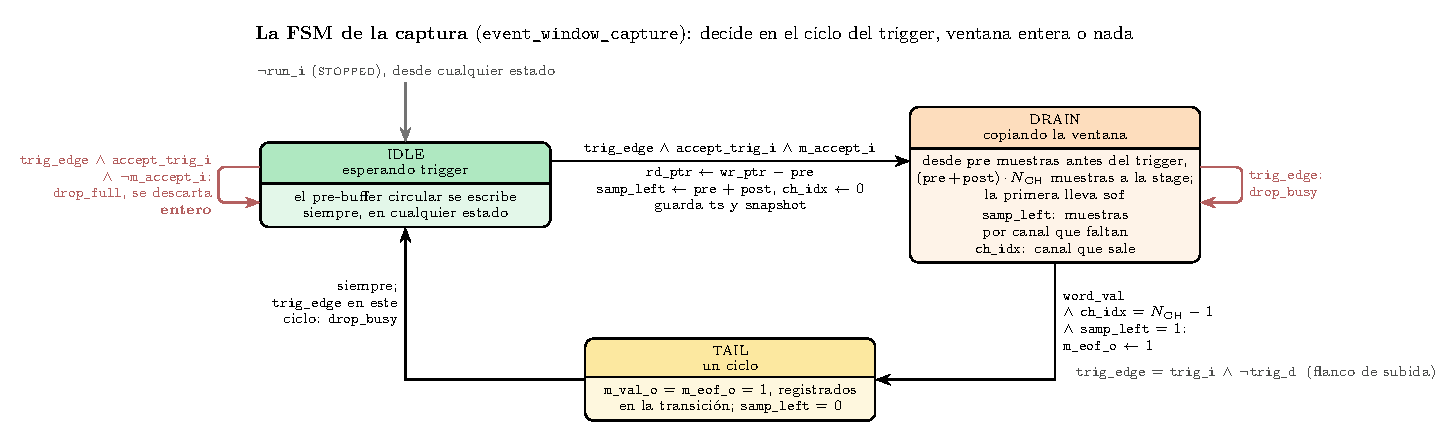
\includegraphics{cap8_fsm_window_capture}
\caption[FSM de captura de un evento]{%
FSM de captura de un evento (\codigo{event\_window\_capture}). Mueve sólo el
lado de lectura del pre-buffer; la escritura sigue en cualquier estado.
\codigo{m\_accept\_i} se mira una sola vez, en el ciclo del trigger: sin lugar,
el evento se descarta entero (\codigo{drop\_full}), y un trigger en
\codigo{DRAIN} o \codigo{TAIL} se pierde como \codigo{drop\_busy}. Con el
anillo en \codigo{RUNNING} todo flanco queda contado:
\codigo{EV\_CNT + DROP\_BUSY + DROP\_FULL} = triggers.\label{f:osc-fsm-window}}
\end{figure}

Mientras que en la Fig.~\ref{f:osc-panorama-window} podemos identificar:
\begin{enumerate}
  \item \textbf{Flanco y decisión} (amarillo):
  \begin{enumerate}
    \item \codigo{trig\_d} guarda el trigger del ciclo anterior y
      \codigo{trig\_edge = trig\_i $\land$ $\lnot$trig\_d}: se toma el flanco y
      no el nivel, porque el disparo por software puede durar más de un ciclo
      de \codigo{adc\_clk} (en placa daba dos eventos por disparo).
    \item \codigo{trig\_edge $\land$ accept\_trig\_i $\land$ idle} es un trigger
      que la captura puede tomar; con \codigo{m\_accept\_i} se separa en
      \codigo{acepta} (carga punteros y metadatos, arranca la FSM) o
      \codigo{drop\_full} (sin lugar aguas abajo, el evento se descarta
      entero).
    \item Un \codigo{trig\_edge} con \codigo{busy} da \codigo{drop\_busy}.
  \end{enumerate}
  \item \textbf{Metadatos} (gris, arriba a la derecha): cuando tenemos
    \codigo{acepta} en alto carga tres registros:
    \codigo{m\_ts $\leftarrow$ ts\_i}, \codigo{m\_snap $\leftarrow$ snapshot\_i}
    y \codigo{m\_nsamp $\leftarrow$ pre\_i + post\_i}, el largo por canal.
  \item \textbf{FSM de ventana} (gris, en el centro): es la de la
    Fig.~\ref{f:osc-fsm-window}.
  \item \textbf{Manejo de punteros y el pre-buffer} (azul):
  \begin{enumerate}
    \item Tenemos una extensión de signo previa de 14 a 16 bits por canal (la
      palabra de los dos canales pasa de 28 a 32 bits).
    \item Se escribe \codigo{pre\_buf[wr\_ptr]} en cada ciclo con
      \codigo{run\_i} y \codigo{dv\_i} en 1.
    \item \codigo{wr\_ptr} suma 1 con cada \codigo{dv\_i}.
    \item El comparador \codigo{rd\_ptr $\neq$ wr\_ptr} da
      \codigo{rd\_avail}.
  \end{enumerate}
  \item \textbf{Pedir palabra}: decide en qué ciclo se lee el pre-buffer. Cada
    palabra trae las $N_\text{CH}$ muestras de un instante, pero la salida
    entrega una por ciclo, así que una palabra alcanza para $N_\text{CH}$
    ciclos.
  \begin{enumerate}
    \item Se pide una palabra cuando no hay ninguna pendiente de serializar
      (\codigo{$\lnot$word\_val}), o cuando la pendiente está entregando su
      último canal (\codigo{ch\_last}): como la lectura tarda un ciclo, la
      palabra nueva llega justo a tiempo y el stream no tiene huecos.
    \item La lectura se hace sólo si hay dato
      (\codigo{do\_read = want\_word $\land$ rd\_avail}); en el post espera a
      que llegue la muestra siguiente.
  \end{enumerate}
  \item \textbf{Contadores de la ventana}: dos registros que usan las regiones
    de pedir palabra y del serializador.
  \begin{enumerate}
    \item \codigo{word\_val}: hay palabra pendiente si se acaba de leer una, o si
      la que estaba todavía tiene canales por entregar.
    \item \codigo{samp\_left}: se carga con \codigo{pre + post} al aceptar y
      baja en uno con cada palabra terminada. Con
      \codigo{samp\_left = m\_nsamp} sale el SOF y con
      \codigo{samp\_left = 1} el EOF; en 0 deja de pedir.
  \end{enumerate}
  \item \textbf{Serializador}:
  \begin{enumerate}
    \item \codigo{word\_r} guarda la palabra leída del pre-buffer (las
      $N_\text{CH}$ muestras de un instante) y un mux elegido por
      \codigo{ch\_idx} saca un canal por ciclo. \codigo{m\_val},
      \codigo{m\_dat}, \codigo{m\_sof} y \codigo{m\_eof} van registrados
      juntos; \codigo{m\_sof} sale con \codigo{ch\_idx = 0} y
      \codigo{samp\_left = m\_nsamp}, y \codigo{m\_eof} con \codigo{ch\_last} y
      \codigo{samp\_left = 1}.
    \item El stream queda con los canales intercalados:
      \codigo{ch0[k], ch1[k], ch0[k+1], \ldots}.
    \item Como se lee una palabra cada $N_\text{CH}$ ciclos y se escribe una por
      ciclo, el rezago entre punteros crece hasta
      $(\text{pre}+\text{post})\cdot N_\text{CH} - \text{post}$. Con $2^{11}$
      palabras entra cualquier ventana de hasta 1024 muestras con
      \codigo{pre} $\leq$ 1023; el bloque no lo verifica, por eso el límite lo
      impone la configuración.
  \end{enumerate}
\end{enumerate}

\begin{figure}[H]
\centering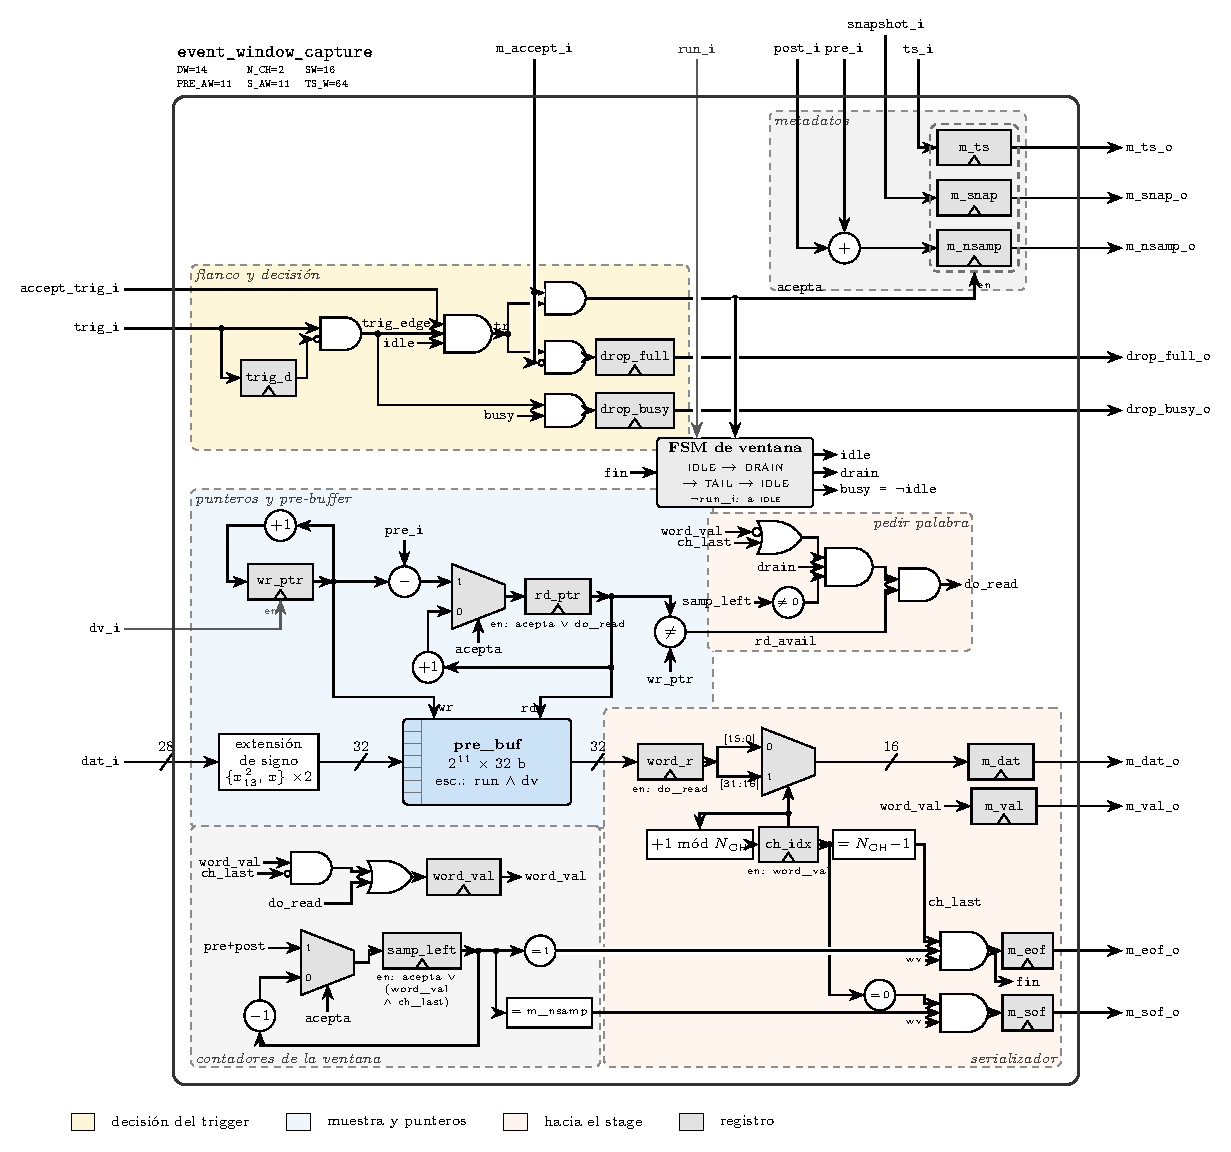
\includegraphics{cap8_panorama_window_capture}
\caption[Vista general de \codigo{event\_window\_capture}]{%
Vista general de \codigo{event\_window\_capture} a nivel de operación. Una sola
memoria guarda el pre y el post: al aceptar, \codigo{rd\_ptr} arranca
\codigo{pre} palabras atrás de \codigo{wr\_ptr}. Desde ahí se lee una palabra
cada $N_\text{CH}$ ciclos mientras el pre-buffer se sigue escribiendo a una por
ciclo. El serializador saca un canal por ciclo con un mux elegido por
\codigo{ch\_idx}. Las redes con nombre se conectan por nombre (\codigo{wv} =
\codigo{word\_val}), y \codigo{NOMBRE=valor} son los parámetros con que lo
instancia \codigo{event\_ring\_top}.\label{f:osc-panorama-window}}
\end{figure}

La FSM de la ventana es muy parecida a la presentada en la
Fig.~\ref{f:ap-osc-fsm-bram}, debido a que tiene el mismo objetivo: segmentar
con un trigger en la entrada un evento dado. Las diferencias ahora son:
\begin{enumerate}
  \item No tenemos un estado de ``armado'', sino que ese bit de información
    (armado/desarmado), que representaba si podíamos sobreescribir el buffer
    interno de los datos, se presenta como entrada del módulo en la señal
    \codigo{m\_accept\_i}: hay lugar aguas abajo para la ventana entera. La
    entrada \codigo{accept\_trig\_i} es otra cosa: la da la FSM global y vale 1
    sólo en \codigo{RUNNING}.
  \item El buffer no se congela: el pre-buffer se escribe siempre y la ventana
    se copia a un stream, así que la captura vuelve a estar lista sin
    intervención del PS.
\end{enumerate}

\subsection{Buffer elástico:
\texorpdfstring{\texttt{event\_stage\_fifo}}{event\_stage\_fifo}}
\label{S:osc-stage-fifo}

Este buffer elástico se denomina \emph{stage} porque no guarda únicamente las
muestras del evento, sino que también tiene una cola de metadatos; las mismas
\textbf{en esta instancia se encuentran desacopladas}. En la
Fig.~\ref{f:osc-panorama-stage} se presenta un diagrama de la misma, que
incluye:
\begin{itemize}
  \item \textbf{Cola de metadatos}: $E = 4$ entradas, con dos punteros
    \codigo{meta\_wr} y \codigo{meta\_rd}; se exporta el nivel presente
    \codigo{ev\_lvl\_o}. El metadato se escribe en el SOF, pero el evento
    \textbf{recién cuenta en el EOF}: \codigo{meta\_lvl} cuenta sólo eventos
    completos y \codigo{meta\_open} marca el que está entrando. Así el escritor
    nunca ve un evento cuyas muestras todavía están llegando, que podría drenar
    más rápido de lo que entran.
  \item \textbf{Cola de muestras}: $2^{12}$ muestras de 16 bits en BRAM, con
    punteros \codigo{wr\_ptr}/\codigo{rd\_ptr} y nivel \codigo{lvl}; cuenta
    cada muestra que entra y sale. La salida está registrada en
    \codigo{dout\_r}, así que la muestra vale un ciclo después del pop.
  \item \textbf{Criterio de aceptación}: requerimos espacio en ambas colas. Con
    \codigo{free \textgreater= win\_len\_i} comprobamos que tenemos el
    suficiente espacio en \codigo{mem}, mientras que \codigo{meta\_full} indica
    si la cola de metadatos puede almacenar otro evento, contando el que está a
    medio entrar.
\end{itemize}

\begin{figure}[H]
\centering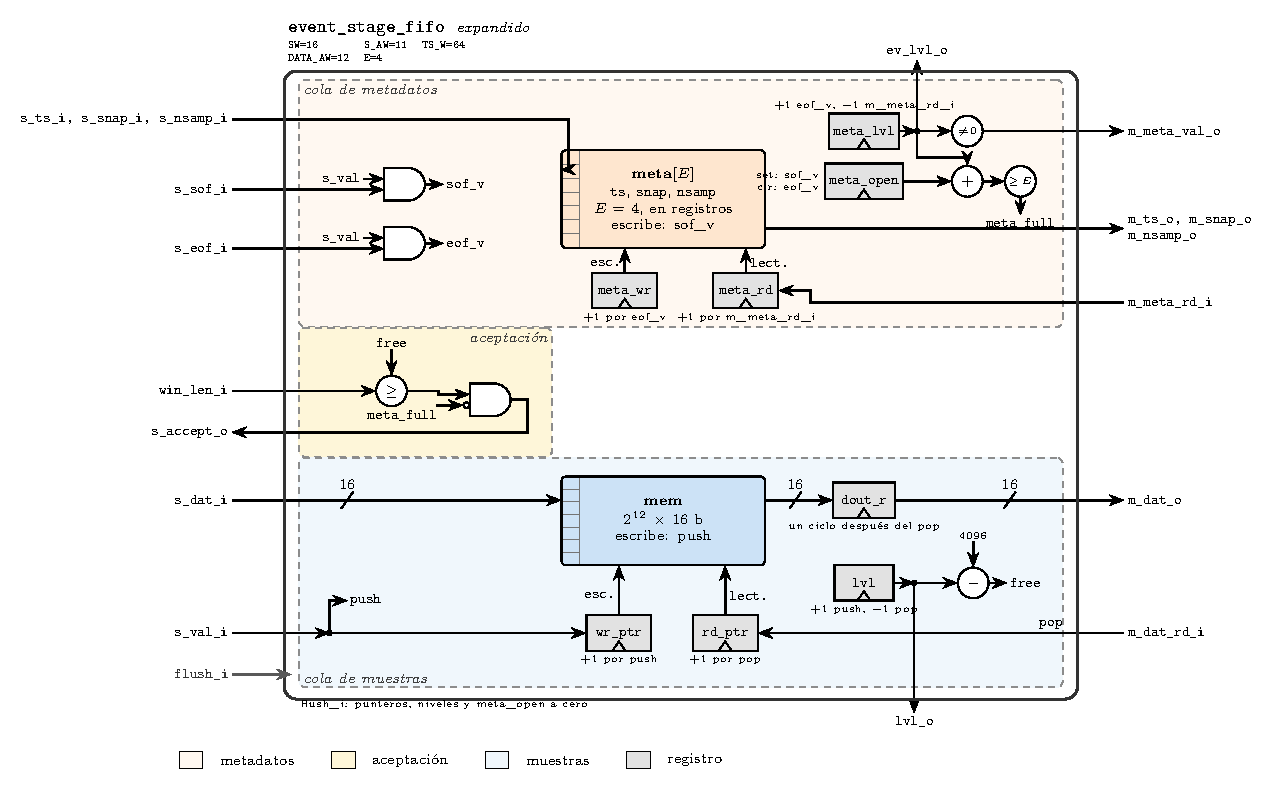
\includegraphics{cap8_panorama_stage_fifo}
\caption[Vista general de \codigo{event\_stage\_fifo}]{%
Vista general de \codigo{event\_stage\_fifo} a nivel de operación. El metadato
se escribe con el SOF, pero el evento recién cuenta con el EOF; así el escritor
no ve un evento cuyas muestras todavía están entrando. Para aceptar hace falta
lugar para la ventana entera y un lugar de metadato, contando el evento a medio
entrar: \codigo{s\_accept\_o = (free $\geq$ win\_len\_i) $\land$
$\lnot$meta\_full}. Con ventanas de 1024 muestras entran dos eventos, no
cuatro.\label{f:osc-panorama-stage}}
\end{figure}

\subsection{Módulo de escritura:
\texorpdfstring{\texttt{event\_slot\_writer}}{event\_slot\_writer}}
\label{S:osc-slot-writer}

Este módulo serializa un evento a un slot del anillo en DDR. Tiene como salida
un AXI-Stream clásico \{\codigo{wr\_data}, \codigo{wr\_val}, \codigo{wr\_rdy}\}
de 64 bits, y escribe exactamente $2^{\text{SLOT\_SHIFT}-3}$ palabras por
evento, en orden de dirección creciente, para que el generador lineal de
direcciones del \codigo{axi\_wr\_fifo} las coloque sin saltos. El layout del
slot se presenta en la Tabla~\ref{t:osc-layout-slot}.

\begin{table}[H]
\centering
\caption[Layout de un slot del anillo en DDR]{%
Layout de un slot del anillo en DDR. Las cuatro primeras palabras (32~B) son la
cabecera, y la cuarta está reservada.\label{t:osc-layout-slot}}
\small
\begin{tabularx}{\textwidth}{|l|>{\raggedright\arraybackslash}X|}
\hline \encabezado \textbf{Offset} & \textbf{Contenido} \\ \hline
\codigo{0x00} & \codigo{timestamp[63:0]}: ticks desde el arranque de la
  corrida \\ \hline
\codigo{0x08} & \codigo{\{flags[7:0], n\_ch[7:0], n\_samp[15:0],
  seq[31:0]\}} \\ \hline
\codigo{0x10} & \codigo{\{32'b0, 15'b0, snapshot[16:0]\}}: qué fuente
  disparó \\ \hline
\codigo{0x18} & reservado (0) \\ \hline
\codigo{0x20} \ldots & muestras int16, 4 por palabra, canales
  \textbf{intercalados}: \codigo{ch0[k], ch1[k], ch0[k+1], \ldots} \\ \hline
\ldots & relleno de ceros hasta la anteúltima palabra \\ \hline
\codigo{SLOT\_SZ $-$ 8} & \textbf{footer}
  \codigo{\{\textasciitilde seq[31:0], seq[31:0]\}} \\ \hline
\end{tabularx}
\end{table}

El footer lleva \codigo{\{\textasciitilde seq, seq\}} para que una lectura rota
o vieja se detecte comparando las dos mitades, sin depender de que el 0 sea un
valor especial. El relleno hace que todos los slots midan lo mismo: la dirección
de un slot se calcula como
\codigo{SLOT\_BASE + (n mod N\_SLOTS)$\cdot$SLOT\_SZ}, sin consultar nada. Si la
ventana no entra en el slot, el escritor la trunca, cierra el slot con su footer
y levanta el sticky \codigo{err\_slot\_ovf}, en vez de pisar el slot siguiente.
Cada palabra se sostiene en la salida hasta que \codigo{axi\_wr\_fifo} la acepta
con \codigo{wr\_rdy\_i}, con el handshake \codigo{valid}/\codigo{ready} de
AXI~\citecap{AMBAAXI}{A3}.

En la Fig.~\ref{f:osc-panorama-writer} se presenta un diagrama general del
módulo. Por simplicidad no expandimos sus bloques, que tienen las siguientes
funciones:
\begin{itemize}
  \item \textbf{Cabecera} (naranja): \codigo{ts}, \codigo{snapshot} y
    \codigo{nsamp} se toman del stage al empezar el evento.
  \item \textbf{Empaquetador} (azul): junta 4 muestras de 16 bits en una
    palabra de 64 bits. Pide una muestra por ciclo, y la que cierra la palabra
    sólo con la salida libre, para no tener que guardar una palabra si la salida
    está ocupada.
  \item \textbf{FSM del slot} (gris): recorre \codigo{W\_IDLE} $\rightarrow$
    \codigo{W\_HDR} $\rightarrow$ \codigo{W\_DATA} $\rightarrow$
    \codigo{W\_PAD} $\rightarrow$ \codigo{W\_FOOT} $\rightarrow$
    \codigo{W\_DONE}, y toma un evento sólo si hay crédito.
  \item \textbf{Palabras del slot} (gris): \codigo{word\_idx} cuenta las
    palabras escritas hasta $2^{\text{SLOT\_SHIFT}-3}-1$, y decide cuándo
    termina el relleno.
  \item \textbf{Mux y salida} (naranja): el estado elige qué palabra sale
    (cabecera, muestras, relleno o footer), y la salida la sostiene hasta
    \codigo{wr\_rdy}.
  \item \textbf{Contadores de slot} (gris): \codigo{wr\_slot} y \codigo{seq}
    suben cuando el FIFO acepta el footer.
\end{itemize}

\begin{figure}[H]
\centering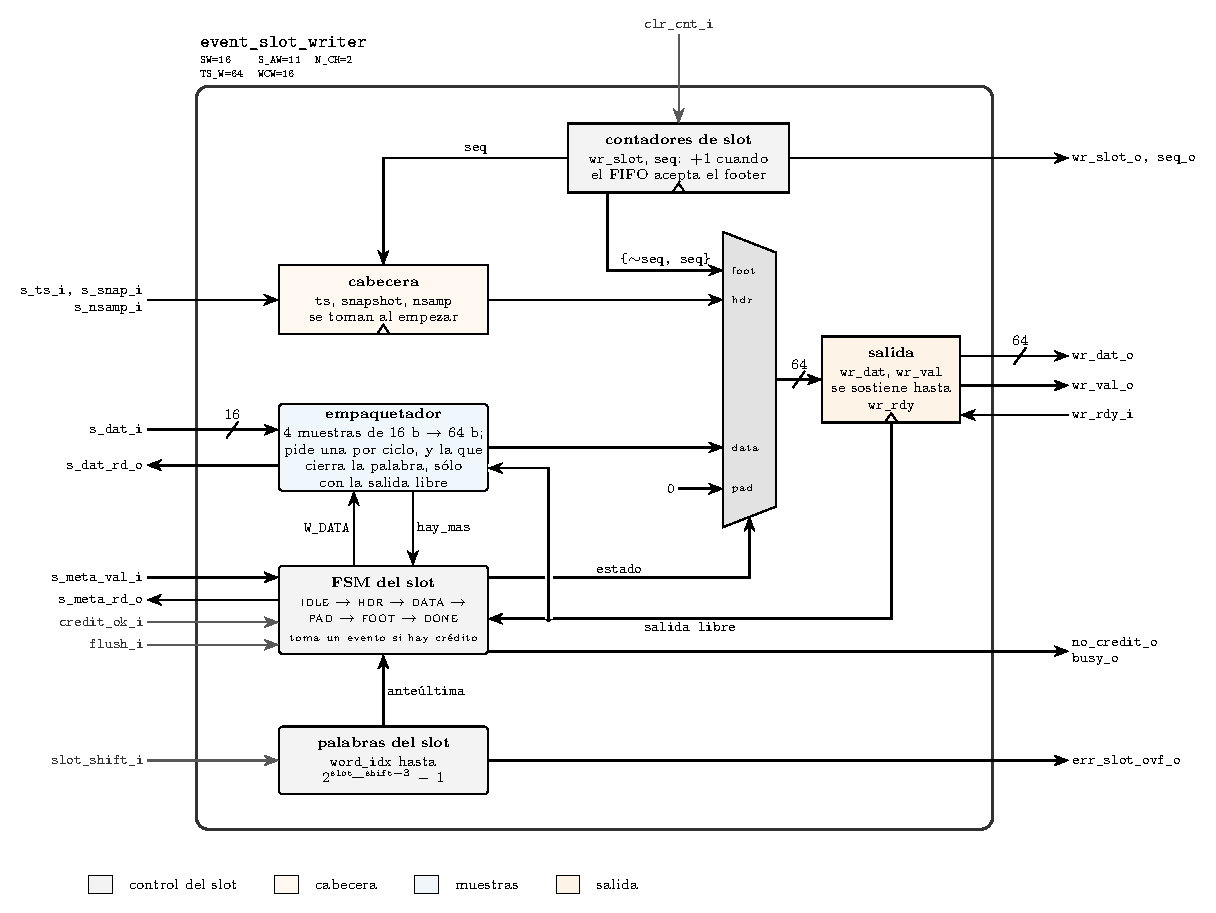
\includegraphics{cap8_panorama_slot_writer}
\caption[Vista general de \codigo{event\_slot\_writer}]{%
Vista general de \codigo{event\_slot\_writer}. El estado de la FSM elige qué
palabra sale: cuatro de cabecera, las muestras empaquetadas de a cuatro, el
relleno de ceros y el footer \codigo{\{\textasciitilde seq, seq\}}. Cada palabra
se sostiene hasta que el \codigo{axi\_wr\_fifo} la acepta, así que la
contrapresión frena al escritor sin perder muestras; \codigo{wr\_slot} y
\codigo{seq} suben recién cuando se acepta el footer.\label{f:osc-panorama-writer}}
\end{figure}

\textbf{FSM del slot}: en la Fig.~\ref{f:osc-fsm-writer} se presenta la FSM de
trabajo, que cuenta con 6 estados que forman un ciclo bajo funcionamiento
típico. El módulo de comprobación de créditos trabaja ciclo a ciclo, y se tiene
la variable \codigo{credit\_ok} en alto cuando los créditos libres son mayores a
cero.
\begin{itemize}
  \item Bajo un reset se va a \codigo{W\_IDLE}, donde espera a tener créditos de
    escritura y un evento completo en la cola de metadatos
    (\codigo{s\_meta\_val}). Con las dos condiciones copia los metadatos,
    calcula el largo del slot y pasa a \codigo{W\_HDR}. Sin créditos \textbf{no
    descarta, se frena}: la contrapresión sube al stage y el descarte ocurre
    arriba, en la captura, donde se puede descartar el evento entero y
    contarlo. \codigo{W\_DONE} da el slot por cerrado cuando el footer fue
    aceptado por el \codigo{axi\_wr\_fifo}: ahí avanzan \codigo{wr\_slot} y
    \codigo{seq}, hace el pop del metadato y vuelve a \codigo{W\_IDLE}.
\end{itemize}
En \codigo{W\_HDR}, \codigo{W\_DATA}, \codigo{W\_PAD} y \codigo{W\_FOOT} cada
palabra espera que el \codigo{axi\_wr\_fifo} la acepte (\codigo{wr\_rdy}) para
continuar con el paso. La lógica interna de la FSM se presenta en la
Fig.~\ref{f:osc-fsm-writer}.

\begin{figure}[H]
\centering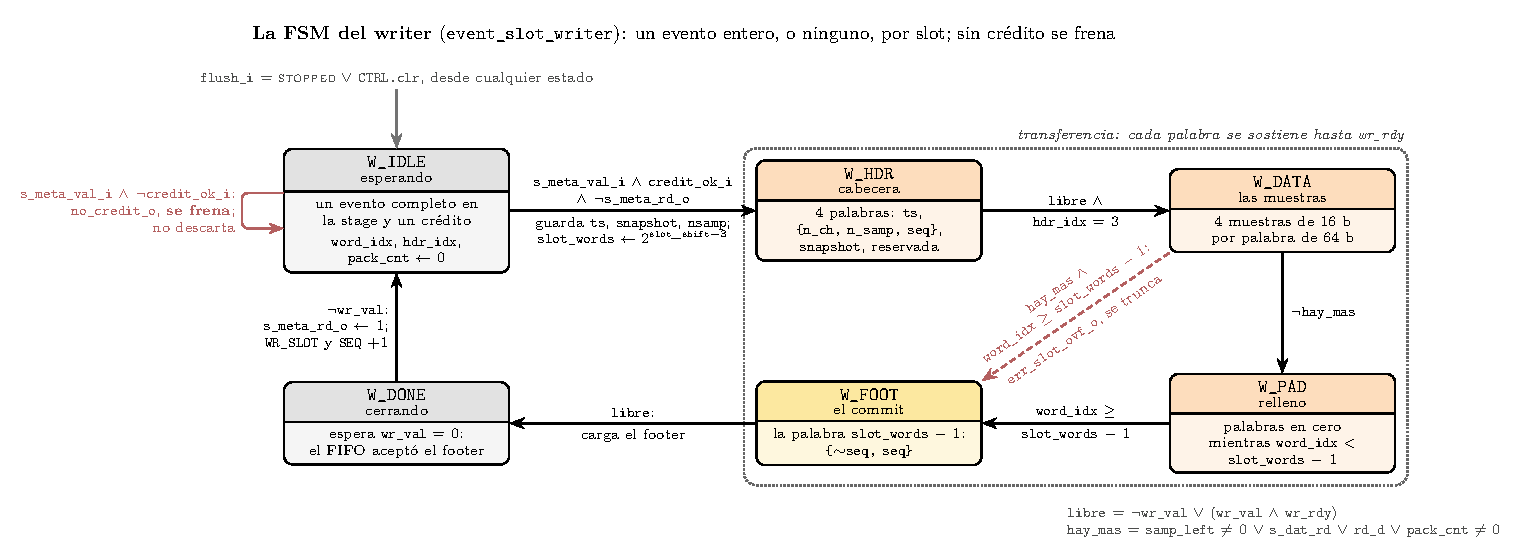
\includegraphics{cap8_fsm_slot_writer}
\caption[FSM del escritor de slots]{%
FSM del escritor de slots. Tiene tres fases: \codigo{W\_IDLE}, la transferencia
(el grupo punteado: \codigo{W\_HDR}, \codigo{W\_DATA}, \codigo{W\_PAD} y
\codigo{W\_FOOT}) y \codigo{W\_DONE}. Sin crédito se queda en \codigo{W\_IDLE}
con \codigo{no\_credit = 1}: se frena, no descarta. En la transferencia cada
palabra se sostiene hasta que el \codigo{axi\_wr\_fifo} la acepta, y el slot se
cierra recién cuando el FIFO acepta el footer.\label{f:osc-fsm-writer}}
\end{figure}

% Bibliografía de este capítulo. Va al final del archivo, siempre.
\bibliografiacapitulo

%%% Local Variables:
%%% mode: latex
%%% TeX-master: "template"
%%% End:
       % Implementación del OSC (señuelo)
% Origen: Secciones/PI - Implementacion TOP (Integracion).md
\chapter{Implementación del TOP (integración)}
\label{C:top}

% Figuras de ESTE capítulo + las compartidas. Siempre al principio del archivo.
\graphicspath{{figs/cap12/}{figs/comunes/}}

\begin{destacado}
Este capítulo habla de (1) qué es y qué incluye un módulo de integración, (2) el
módulo base original de Pitaya, versión 0.94, en el que nos basamos, y los
cambios aplicados, (3) los posibles caminos que puede tener el datapath y (4)
los registros de configuración del mismo~\cite{RedPitayaFPGA}.
\end{destacado}

%==============================================================================
\section{Sistema base de Pitaya: módulo de integración}
\label{S:top-sistema-base}

Este es el archivo cabecera (TOP) del diseño, y es el responsable de:
\begin{itemize}
  \item Tener como entradas y salidas las interfaces de los periféricos
    externos.
  \item Instanciar macros de recursos de clock y macros de periféricos
    empleados, por ejemplo el PS.
  \item Armar las \textbf{redes de reloj} (\emph{clock domains}) y las
    \textbf{redes de reset} (\emph{reset domains}).
  \item \textbf{Instanciar los módulos e interconectarlos}.
  \item \textbf{Instanciar el bus interno} e interconectarlo mediante un bridge
    al PS.
\end{itemize}

\subsection{Vista general del TOP}
\label{S:top-vista-general}

La documentación oficial~\cite{RedPitayaDocs} presenta el esquema ASCII del
TOP, mientras que el nuestro, \codigo{event\_ring\_red\_pitaya\_top}, se presenta en la
Fig.~\ref{f:top-panorama} y está constituido por los siguientes subsistemas:
\begin{itemize}
  \item \textbf{Módulo del PS}: \codigo{red\_pitaya\_ps}, que pertenecía al
    sistema original de Pitaya.
  \begin{itemize}
    \item Toma las señales físicas del módulo e instancia estructuras que las
      representan.
  \end{itemize}
  \item \textbf{Bridges PS-PL}: el PS y la PL se comunican por dos
    caminos~\cite{UG585}.
  \begin{itemize}
    \item \textbf{Control}, por el puerto maestro M\_AXI\_GP0 del PS. Del lado de
      la PL lo recibe \codigo{axi4\_slave}, que traduce las transacciones
      AXI4-Lite de 32 bits~\cite{AMBAAXI} al handshake del bus custom. Es el
      camino lento, el que usa el ARM para leer y escribir registros.
    \item \textbf{Datos}, por los puertos esclavos S\_AXI\_HP del PS. Del lado
      de la PL los maneja \codigo{axi\_master}, que convierte las escrituras del
      bus custom en ráfagas AXI4 de 64 bits hacia la DDR, sin pasar por el ARM.
      Se usa sólo HP2, por el que el \codigo{event\_ring} escribe sus ventanas.
      HP0 y HP1, los de la captura del OSC a DDR, y HP3 quedan en cero.
  \end{itemize}
  \item \textbf{Interconnect del bus custom}: los detalles de la interfaz y las
    secuencias que utiliza el bus custom se presentan en la
    Sec.~\ref{S:intro-hw-bus-custom}. El interconnect,
    \codigo{sys\_bus\_interconnect}, reparte cada transacción del PS al módulo
    que corresponde.
  \begin{itemize}
    \item Está instanciado de forma que subdivide el espacio de direcciones en 8
      regiones de igual tamaño, de 1~MiB cada una a partir de
      \codigo{0x4000\_0000}. Estas se presentan en la
      Tabla~\ref{t:top-slots}.
  \end{itemize}
\end{itemize}

\begin{figure}[H]
\centering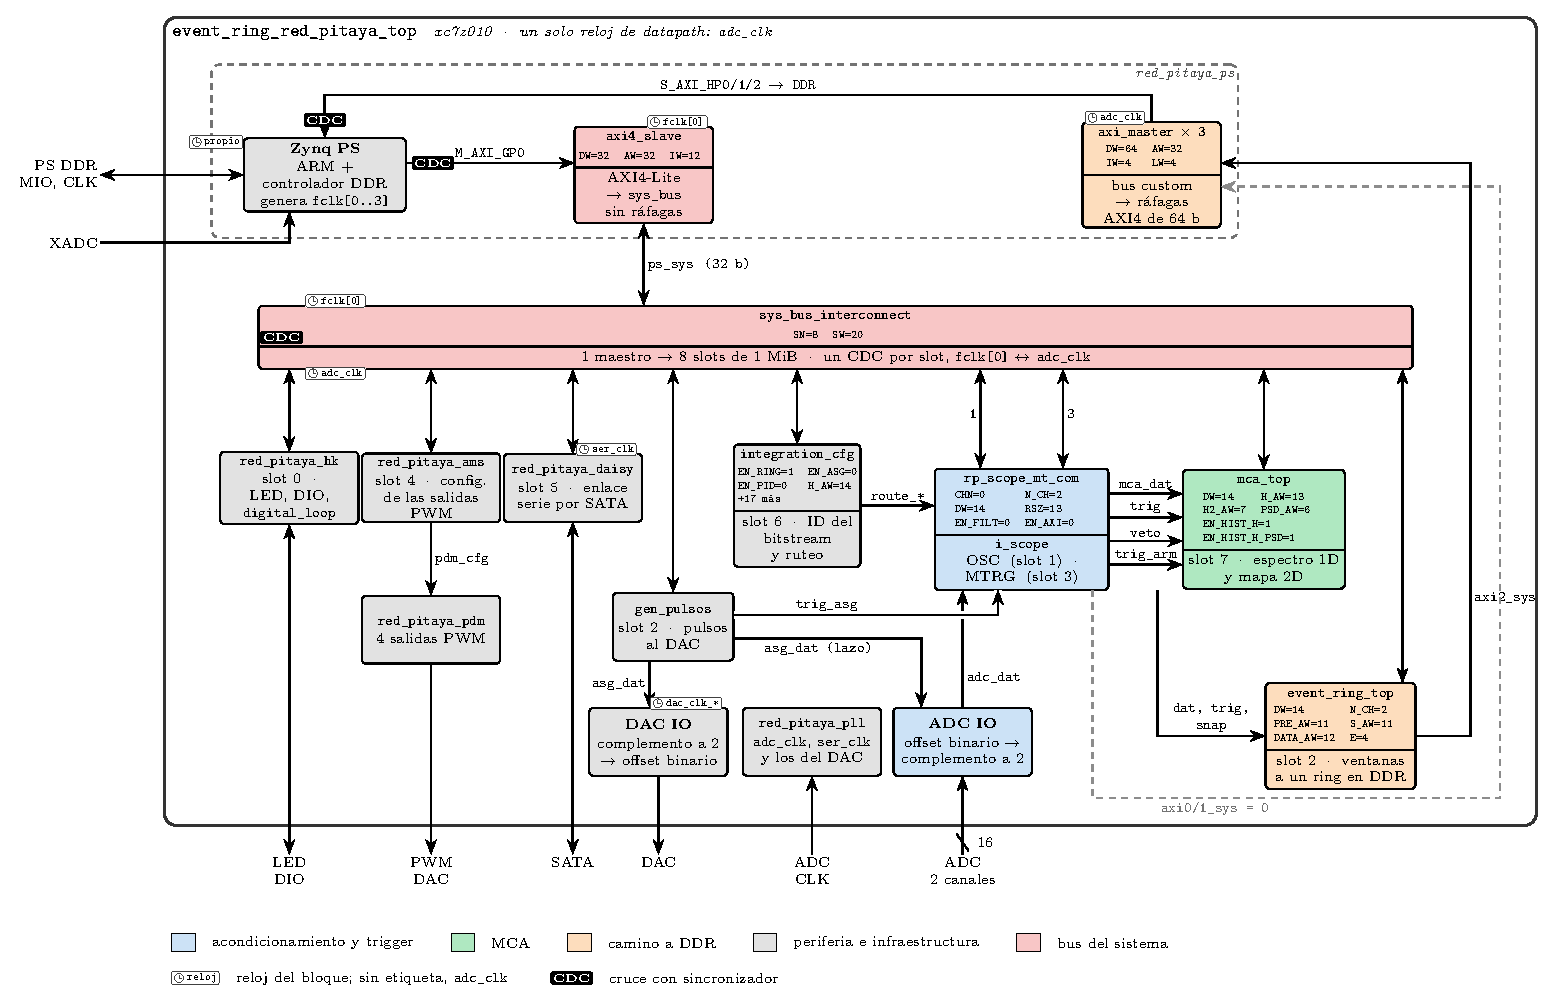
\includegraphics{cap12_panorama_top}
\caption[Diagrama general del TOP del sistema]{%
Diagrama general del TOP del sistema. Los pines físicos quedan en el borde.
Control: GP0 $\rightarrow$ \codigo{sys\_bus}. Datos: \codigo{event\_ring\_top}
$\rightarrow$ HP2 $\rightarrow$ DDR, sin pasar por el ARM; la captura del OSC a
DDR no está (\codigo{EN\_AXI=0}) y \codigo{axi0/1\_sys} quedan en cero.
\codigo{NOMBRE=valor}: parámetros con que el padre instancia el bloque (se
omiten los que sólo pasan el del padre sin cambio). En \codigo{integration\_cfg}
se muestran 4 de sus 21. Las etiquetas con reloj marcan los bloques que no
corren en \codigo{adc\_clk}, o que podrían confundirse: \codigo{axi\_master}
está dentro del PS pero corre en \codigo{adc\_clk}. \codigo{CDC} marca los
cruces que necesitan sincronizador: el interconnect, uno por slot, entre
\codigo{fclk[0]} y \codigo{adc\_clk}, que tienen la misma frecuencia nominal
pero salen de osciladores distintos, y los puertos GP0 y HP, que cruza el propio
PS. El slot 2 lo comparten el \codigo{event\_ring} (\codigo{0x4020\_0000}) y
\codigo{gen\_pulsos} (\codigo{0x4021\_0000}), que maneja el DAC, la fuente ASG
del multitrigger y, con \codigo{digital\_loop[0]}, la entrada de la cadena en
lugar del ADC.\label{f:top-panorama}}
\end{figure}

\begin{table}[H]
\centering
\caption[Regiones del bus custom]{%
Regiones del bus custom en \codigo{event\_ring\_red\_pitaya\_top}. Los slots 1
y 3 son dos buses de la misma instancia, \codigo{rp\_scope\_mt\_com}, que expone
por separado los registros del osciloscopio y los del multitrigger. El slot 2
lo reparte \codigo{sys\_bus\_split}: los 64~kB de \codigo{0x4021\_0000} van a
\codigo{gen\_pulsos} y el resto al \codigo{event\_ring}.\label{t:top-slots}}
\small
\begin{tabularx}{\textwidth}{|c|l|>{\raggedright\arraybackslash}X%
  |>{\raggedright\arraybackslash}p{0.22\textwidth}|}
\hline \encabezado \textbf{Slot} & \textbf{Base} & \textbf{Módulo} &
  \textbf{Origen} \\ \hline
0 & \codigo{0x4000\_0000} & \codigo{red\_pitaya\_hk}: LEDs, DIO y lazo digital
  & Red Pitaya \\ \hline
1 & \codigo{0x4010\_0000} & osciloscopio (\codigo{rp\_scope\_mt\_com}) & Red
  Pitaya, modificado \\ \hline
2 & \codigo{0x4020\_0000} & \codigo{event\_ring} en \codigo{0x4020\_0000};
  \codigo{gen\_pulsos} en \codigo{0x4021\_0000} & propio, en lugar del ASG
  \\ \hline
3 & \codigo{0x4030\_0000} & multitrigger (\codigo{rp\_scope\_mt\_com}) &
  propio, en lugar del PID \\ \hline
4 & \codigo{0x4040\_0000} & \codigo{red\_pitaya\_ams}: XADC y PDM & Red Pitaya
  \\ \hline
5 & \codigo{0x4050\_0000} & \codigo{red\_pitaya\_daisy}: enlace serie por los
  conectores SATA & Red Pitaya \\ \hline
6 & \codigo{0x4060\_0000} & \codigo{integration\_cfg}: identificación y ruteo &
  propio \\ \hline
7 & \codigo{0x4070\_0000} & MCA (\codigo{mca\_top}) & propio \\ \hline
\end{tabularx}
\end{table}

Si expandimos el \codigo{sys\_bus\_interconnect}
(Fig.~\ref{f:top-interconnect}), vemos que toma \codigo{addr[22:20]} y lo
convierte en un chip select \codigo{CS} en formato one-hot, que se combina con
una AND (\&) para asegurar que la request llegue únicamente al slot deseado. A
la vuelta hay simplemente un MUX cuyo selector es el mismo
\codigo{addr[22:20]}.

\begin{figure}[H]
\centering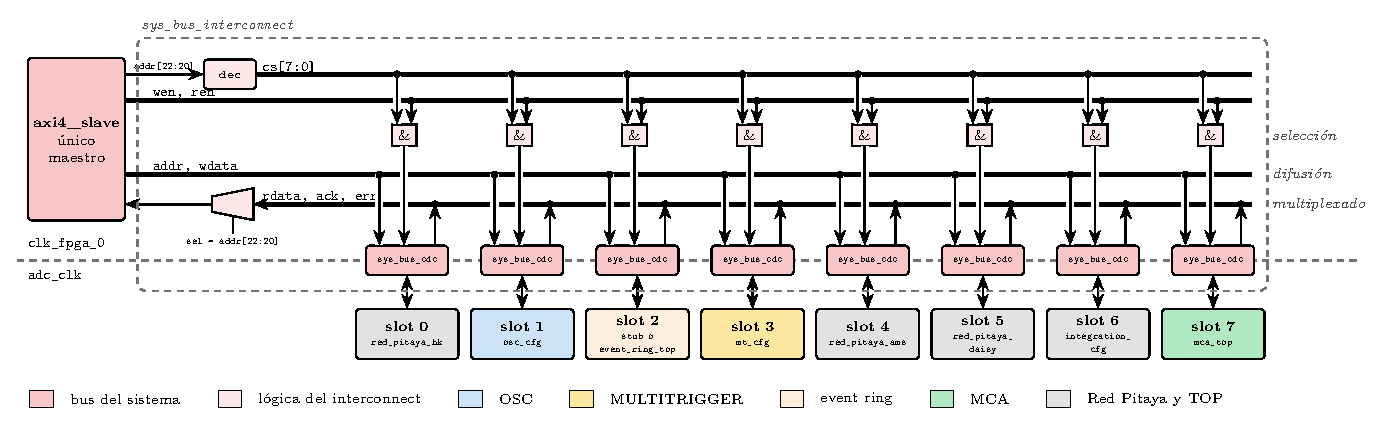
\includegraphics{cap12_estructura_sys_bus}
\caption[Interconnect principal del bus custom de Pitaya]{%
Esquema del interconnect principal del bus custom de Pitaya: una topología en
estrella en la que \codigo{axi4\_slave} es el único maestro y los ocho slots son
los esclavos.\label{f:top-interconnect}}
\end{figure}

\subsection{Cambios realizados en el TOP original}
\label{S:top-cambios}

\begin{sloppypar}
Nuestro TOP, \codigo{event\_ring\_red\_pitaya\_top}, parte del TOP del proyecto
(\codigo{red\_pitaya\_top}, el de Red Pitaya con el osciloscopio ya
reemplazado por \codigo{rp\_scope\_mt\_com}). Las diferencias son:
\end{sloppypar}
\begin{enumerate}
  \item \textbf{El MCA en el slot 7} (\codigo{0x4070\_0000}).
  \item \textbf{Sin ecualizador} (\codigo{EN\_FILT = 0}): su lazo IIR no cierra
    timing a \qty{125}{\mega\hertz}.
  \item \textbf{Sin generador arbitrario (ASG)} en el slot 2. Su lugar lo
    comparten dos módulos, que reparte \codigo{sys\_bus\_split}: el
    \codigo{event\_ring} (\codigo{0x4020\_0000}), que escribe sus ventanas a la
    DDR por HP2, y \codigo{gen\_pulsos} (\codigo{0x4021\_0000}), que maneja la
    entrada del DAC y la fuente de disparo ASG del multitrigger.
  \item \textbf{Sin captura del OSC a DDR} (\codigo{EN\_AXI = 0}): la reemplaza
    el \codigo{event\_ring}, y HP0 y HP1 quedan en cero. La captura por BRAM del
    OSC sigue.
  \item \textbf{Sin PID} en el slot 3, que no se usa en este flujo. En su lugar
    va el multitrigger, que en \codigo{red\_pitaya\_top} ocupa el slot 7.
  \item \textbf{\codigo{integration\_cfg} en el slot 6} y un selector de nodo por
    consumidor en el datapath (Sec.~\ref{S:top-registros}).
\end{enumerate}

Se conservan a propósito la lista de puertos y los nombres de instancia
\codigo{i\_ams} y \codigo{sys\_bus\_interconnect}, porque las restricciones del
XDC se enganchan por esos nombres.

\subsection{Redes de reloj y de reset}
\label{S:top-relojes}

El TOP arma dos familias de relojes (Tabla~\ref{t:top-relojes}). La primera nace
del ADC: el oscilador de la placa maneja al ADC y entra a la PL, a
\qty{125}{\mega\hertz}, por el par diferencial \codigo{adc\_clk\_i}. Con él se
alimenta una PLL~\cite{UG472} (\codigo{red\_pitaya\_pll}), de la que salen, por
buffers globales (BUFG), el reloj de la adquisición, los del DAC y el del enlace
serie. Todo el procesamiento propio (OSC, MT, MCA, \codigo{gen\_pulsos},
\codigo{event\_ring} e \codigo{integration\_cfg}) corre en \codigo{adc\_clk},
así que la muestra no cruza ningún dominio de reloj entre el ADC y el histograma
o el anillo. También corre en \codigo{adc\_clk} el \codigo{axi\_master} de HP2,
aunque esté dentro del módulo del PS. La segunda familia nace en el PS, que
genera sus relojes con sus propios PLL a partir de otro oscilador:
\codigo{fclk[0]}, de \qty{125}{\mega\hertz}, con el que corre el lado PS del
bus, y \codigo{fclk[3]}, de \qty{200}{\mega\hertz}, que usa el enlace serie para
los retardos de entrada (IDELAY). En la Fig.~\ref{f:top-panorama} cada bloque
lleva su reloj cuando no es \codigo{adc\_clk}, y los cruces que necesitan
sincronizador están marcados.

\begin{table}[H]
\centering
\caption[Relojes del TOP]{%
Relojes del TOP. Los de la PLL salen todos del reloj del ADC y guardan relación
de fase entre sí; los del PS, no. La PLL genera además un reloj de PWM que en
este TOP no usa ningún bloque: el PDM corre en \codigo{adc\_clk}. La recepción
del enlace serie usa el reloj que llega del otro extremo por el cable
SATA.\label{t:top-relojes}}
\small
\begin{tabularx}{\textwidth}{|>{\raggedright\arraybackslash}p{0.25\textwidth}%
  |>{\raggedright\arraybackslash}p{0.2\textwidth}|c%
  |>{\raggedright\arraybackslash}X|}
\hline \encabezado \textbf{Reloj} & \textbf{Frecuencia} & \textbf{Origen} &
  \textbf{Lo usa} \\ \hline
\codigo{adc\_clk} & \qty{125}{\mega\hertz} & PLL & adquisición,
  procesamiento, lado PL del bus y puerto HP2 \\ \hline
\codigo{dac\_clk\_1x} & \qty{125}{\mega\hertz} & PLL & DAC: datos de los dos
  canales intercalados, selección y reset \\ \hline
\codigo{dac\_clk\_2x}, \codigo{dac\_clk\_2p} & \qty{250}{\mega\hertz}; el
  segundo, a $-45^\circ$ & PLL & DAC: escritura y reloj de salida \\ \hline
\codigo{ser\_clk} & \qty{250}{\mega\hertz} & PLL & enlace serie
  (\codigo{red\_pitaya\_daisy}), transmisión \\ \hline
\codigo{fclk[0]} & \qty{125}{\mega\hertz} & PS & lado PS del bus
  (\codigo{axi4\_slave}) \\ \hline
\codigo{fclk[3]} & \qty{200}{\mega\hertz} & PS & retardos de entrada del enlace
  serie \\ \hline
\end{tabularx}
\end{table}

Aunque \codigo{fclk[0]} y \codigo{adc\_clk} tienen la misma frecuencia nominal,
no salen de la misma PLL: cada uno viene de su propio oscilador. Son relojes
\textbf{plesiócronos}~\cite{Dally1998}: tienen la misma frecuencia nominal, pero
cada oscilador tiene su tolerancia y su deriva, así que la fase entre los dos se
corre lentamente y, con el tiempo, pasa por todos los valores. No se les puede
suponer ninguna relación de fase fija, y el cruce necesita un sincronizador
general, el mismo que haría falta entre dos relojes sin ninguna relación. Si
salieran de la misma PLL serían sincrónicos y alcanzaría con el análisis de
timing, como pasa entre \codigo{adc\_clk} y los relojes del DAC.

El cruce lo hace el interconnect, con un \codigo{sys\_bus\_cdc} por slot que pasa
cada transacción de \codigo{fclk[0]} a \codigo{adc\_clk} y su respuesta de
vuelta, por un handshake con sincronizadores de varios
flip-flops~\cite{Cummings2008}. Por eso el bus admite una transacción a la vez
por slot y cada acceso se lleva unos pocos ciclos. Las restricciones del XDC no
suponen ninguna relación de fase entre los dos relojes: sólo acotan, a un
período, el retardo del camino hasta el primer flip-flop de cada sincronizador.
La respuesta de lectura cruza registrada: el esclavo deja el dato fijo en el
ciclo del ack y \codigo{sys\_bus\_cdc} lo congela antes de pasarlo al PS. Los
otros dos cruces los resuelve el propio PS en sus puertos~\cite{UG585}: GP0
corre en \codigo{fclk[0]} y HP2 en \codigo{adc\_clk}, y el PS pasa cada
transacción a sus relojes internos.

Cada dominio tiene su propio reset (\codigo{adc\_rstn}, \codigo{dac\_rst},
\codigo{dac\_axi\_rstn}, \codigo{pwm\_rstn}), registrado en su reloj. Todos salen
de \codigo{frstn[0]}, el reset de la PL que maneja el PS, y del enganche de la
PLL: el reset se mantiene activo mientras el PS mantenga \codigo{frstn[0]} y
durante una cuenta de ciclos después de que la PLL engancha, así ningún módulo
arranca con el reloj todavía inestable. Si la PLL pierde el enganche, el TOP la
resetea desde el dominio de \codigo{fclk[0]}, que no depende de ella. El estado
de \codigo{pll\_locked} y de \codigo{adc\_rstn} se puede leer desde
\codigo{integration\_cfg}.

\subsection{Datapath y cálculo de tiempo muerto en integración}
\label{S:top-datapath}

En la Fig.~\ref{f:top-datapath} se presentan los flujos principales de datos
dentro de la integración.

\begin{figure}[H]
\centering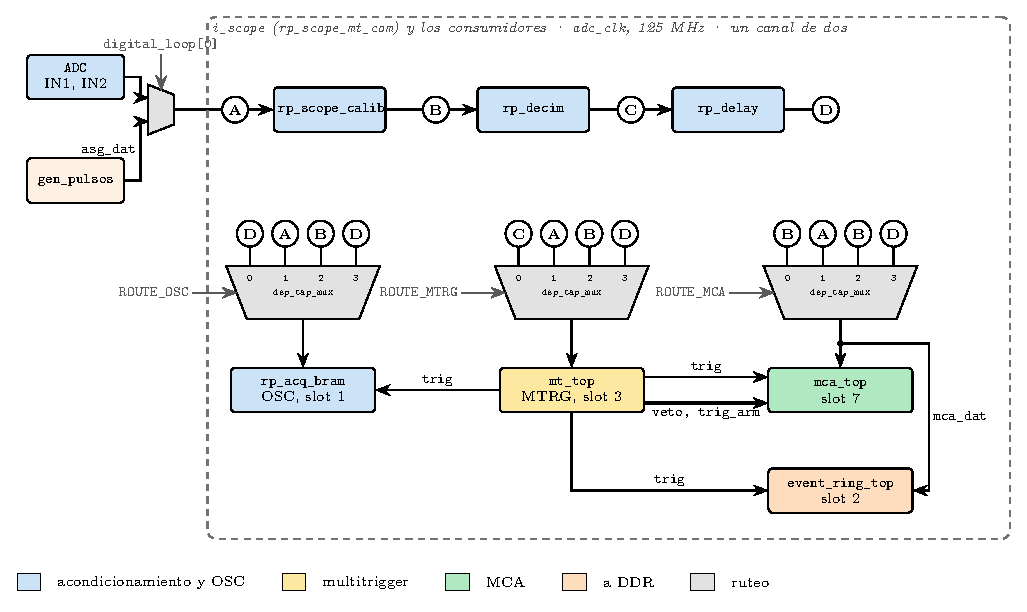
\includegraphics{cap12_datapath_top}
\caption[Datapath del módulo de integración]{%
Datapath del módulo de integración. Hay una sola cadena de acondicionado por
canal (calibración, diezmado, retardo) con cuatro nodos (A a D). El OSC, el
multitrigger y el MCA tienen cada uno su \codigo{dsp\_tap\_mux} 4:1, que elige
en runtime con su \codigo{ROUTE\_*}; cada entrada lleva su código de tap (0 a 3)
y la letra del nodo, y la 0 es el nodo nativo, el valor de reset. El
\codigo{event\_ring} no tiene selector: toma lo mismo que el MCA
(\codigo{mca\_dat}). A la izquierda, el lazo digital: con
\codigo{digital\_loop[0]} la cadena toma los pulsos de \codigo{gen\_pulsos} en
lugar del ADC. Abajo, lo que el multitrigger da a los otros consumidores: el
flanco \codigo{trig} a los tres, y \codigo{veto} y \codigo{trig\_arm}, niveles,
sólo al MCA.\label{f:top-datapath}}
\end{figure}

Hay una sola cadena de acondicionamiento por canal: calibración de ganancia y
offset (\codigo{rp\_scope\_calib}), diezmado (\codigo{rp\_decim}) y retardo de
disparo (\codigo{rp\_delay}). El ecualizador del proyecto de Red Pitaya
(\codigo{osc\_filter}) no está en nuestro TOP (\codigo{EN\_FILT = 0}), porque su
lazo IIR no cierra timing a \qty{125}{\mega\hertz}, y tampoco la captura del OSC
a DDR (\codigo{EN\_AXI = 0}), que reemplaza el \codigo{event\_ring}. Los
consumidores (OSC, MT, MCA y \codigo{event\_ring}) no tienen una cadena cada
uno: toman la muestra de uno de los cuatro nodos de esa misma cadena
(Tabla~\ref{t:top-nodos}). Para eso el OSC, el MT y el MCA tienen cada uno su
propio selector 4:1, \codigo{dsp\_tap\_mux}, que el software configura en tiempo
de ejecución con los registros \codigo{ROUTE\_*} de \codigo{integration\_cfg}.
Son tres selectores independientes, no una matriz de conmutación. El
\codigo{event\_ring} no tiene selector propio: toma la misma muestra que el MCA.
La entrada 0 de cada selector es el nodo \textbf{nativo}, el que el consumidor
tenía cableado antes de que existiera el selector, y es el valor de reset: sin
configurar nada, el datapath es idéntico al original.

\begin{table}[H]
\centering
\caption[Nodos de la cadena de acondicionamiento]{%
Nodos de la cadena de acondicionamiento; $R$ es el factor de diezmado. Cada nodo
es un prefijo de la misma cadena. El C sólo lo alcanza el MT, como nativo, y por
eso no tiene código de \codigo{tap\_sel}.\label{t:top-nodos}}
\small
\begin{tabularx}{\textwidth}{|c|l|>{\raggedright\arraybackslash}X|l|c%
  |>{\raggedright\arraybackslash}p{0.17\textwidth}|}
\hline \encabezado \textbf{Nodo} & \textbf{Señal} & \textbf{Etapas que acumuló}
  & \textbf{Ritmo} & \codigo{tap\_sel} & \textbf{Nativo de} \\ \hline
A & \codigo{adc\_calib\_in} & ninguna: la muestra cruda & 125~MSPS & 1 & ---
  \\ \hline
B & \codigo{adc\_dec\_in} & calibración & 125~MSPS & 2 & MCA y
  \codigo{event\_ring} \\ \hline
C & \codigo{adc\_dly\_in} & + diezmado & $125/R$~MSPS & --- & MT \\ \hline
D & \codigo{adc\_bram\_in} & + retardo & $125/R$~MSPS & 3 & OSC \\ \hline
\end{tabularx}
\end{table}

El selector arrastra el par (dato, valid): los nodos posteriores al diezmado
entregan una muestra cada $R$ ciclos con su estrobo, y los consumidores lo
respetan. Es combinacional a propósito: registrarlo correría el dato un ciclo
respecto de las señales de control de cada consumidor y, en modo nativo, el
hardware dejaría de ser idéntico al original.

Hay dos consecuencias para el uso. Como el \codigo{event\_ring} toma lo mismo
que el MCA, \codigo{ROUTE\_MCA} mueve a los dos. Y el MT toma por defecto el nodo
C, posterior al diezmado, así que diezmar para ver una ventana más larga en el
OSC también diezma la señal con la que se disparan el MCA y el ring, salvo que
se cambie \codigo{ROUTE\_MTRG}.

A la izquierda de la Fig.~\ref{f:top-datapath} está el lazo digital: con el bit
0 de \codigo{digital\_loop}, en \codigo{red\_pitaya\_hk}, la cadena toma los
pulsos de \codigo{gen\_pulsos} en lugar de las muestras del ADC, y todo el
datapath ve el estímulo del generador sin pasar por la etapa analógica.

\subsection{Registros de integración}
\label{S:top-registros}

El slot 6 lo ocupa \codigo{integration\_cfg}, un módulo propio que no existe en
el proyecto de Red Pitaya. Su función es que el software \textbf{descubra} el
sistema en lugar de suponerlo: qué bitstream está cargado, qué módulos trae y en
qué slot vive cada uno. Hace falta porque el mapa no es el mismo en todos los
bitstreams del proyecto. Sus registros se agrupan en cuatro bloques
(Tabla~\ref{t:top-registros}).

\begin{table}[H]
\centering
\caption[Bloques de registros de \codigo{integration\_cfg}]{%
Bloques de registros de \codigo{integration\_cfg} (base
\codigo{0x4060\_0000}).\label{t:top-registros}}
\small
\begin{tabularx}{\textwidth}{|>{\raggedright\arraybackslash}p{0.2\textwidth}%
  |>{\raggedright\arraybackslash}p{0.2\textwidth}%
  |>{\raggedright\arraybackslash}X|}
\hline \encabezado \textbf{Bloque} & \textbf{Offset} & \textbf{Contenido}
  \\ \hline
Identificación & \codigo{0x000}--\codigo{0x018} & \codigo{MAGIC}
  (\codigo{\textquotedbl INTG\textquotedbl}), versión y hash de git del commit
  del que salió el bitstream (160 bits) \\ \hline
Descripción del sistema & \codigo{0x020}--\codigo{0x02C} & \codigo{MODULES}
  (qué módulos hay), \codigo{SLOTS} (en qué slot está cada uno) y
  \codigo{CAPS\_*} (parámetros de síntesis: canales, anchos, tamaños de los
  histogramas) \\ \hline
Ruteo del datapath & \codigo{0x030}--\codigo{0x03C} & \codigo{ROUTE\_OSC},
  \codigo{ROUTE\_MTRG} y \codigo{ROUTE\_MCA}: nodo de cada consumidor
  (\codigo{[1:0]}) y habilitación (\codigo{[8]}). \codigo{ROUTE\_RING} existe
  pero no está conectado \\ \hline
Control global & \codigo{0x040}--\codigo{0x044} & \codigo{run},
  \codigo{clear} y \codigo{soft\_reset}, todavía sin consumidores; estado de
  \codigo{pll\_locked} y \codigo{adc\_rstn} \\ \hline
\end{tabularx}
\end{table}

Los registros de identificación y de descripción salen de parámetros de
síntesis, así que no cuestan flip-flops: son constantes cableadas al
multiplexor de lectura. El hash de git lo inyecta el script de construcción como
parámetro, de modo que el bitstream sabe de qué commit salió sin que nadie lo
anote. \codigo{libmca} lee estos registros para calcular la dirección de cada
módulo (Sec.~\ref{S:sw-libmca}).

% Bibliografía de este capítulo. Va al final del archivo, siempre.
\bibliografiacapitulo

%%% Local Variables:
%%% mode: latex
%%% TeX-master: "template"
%%% End:
      % Implementación del TOP (integración)
% Origen: Secciones/PI - Software.md
% Su sección "Apéndice" está en apend5.tex (Complementos del software).
\chapter{Software}
\label{C:sw}

% Figuras de ESTE capítulo + las compartidas. Siempre al principio del archivo.
\graphicspath{{figs/cap10/}{figs/comunes/}}

\begin{destacado}
En este capítulo se desarrolla el software que corre en el procesador de la
placa y en la PC. (1) Partimos de la diferenciación primordial entre el espacio
del \emph{kernel} y el espacio de usuario, y de la elección del sistema operativo: como
los requerimientos de latencia quedaron en el PL, usamos el Linux de la
distribución de Red Pitaya, y todo nuestro software corre en el espacio de
usuario, sobre \ruta{/dev/mem}, evitando los modos de falla del bus. (2)
Presentamos la API en seis capas, desde el mapeo crudo de la memoria hasta las
aplicaciones, y su núcleo en C, \codigo{libmca}, con un \emph{handle} por cada bloque
del PL y un \emph{binding} a Python. (3) Describimos cómo se guardan las adquisiciones:
los espectros del MCA en \ruta{.csv}, N42.42 o \ruta{.npz}, y las trazas del
osciloscopio en archivos de un \emph{batch} cada uno, que la sesión de captura escribe
con dos hilos, un lector y un escritor, que se pasan un \emph{pool} de \emph{batches}. (4)
Presentamos el protocolo de red entre la placa y la PC, y el modo de exportación
del ring, en el que la placa manda los eventos por TCP y la PC arma los
archivos. (5) Por último, medimos el costo de las llamadas a \codigo{libmca} y
la escritura persistente de trazas: por red pasan entre 2.2 y 3.5 veces más
eventos que a la SD de la placa.
\end{destacado}

%==============================================================================
\section{Capas de software}
\label{S:sw-capas}

Nuestro sistema cuenta con múltiples capas de SW; mientras más capas tenemos,
generalmente tenemos más acceso a abstracciones que vuelven el desarrollo más
encarable. La diferencia fundamental está en subdividirlo en dos grandes
secciones: el \textbf{espacio del \emph{kernel}} del sistema operativo (OS) y el
\textbf{espacio de usuario}.

La diferencia fundamental se encuentra en el \textbf{nivel de privilegio de
ejecución}: dentro de ARMv7-A tenemos dos, privilegiado (PL1) y no privilegiado
(PL0). En la Tabla~\ref{t:sw-kernel-usuario} se muestran las diferencias más
importantes.

% En la nota la tabla no tiene epígrafe: este es provisorio.
\begin{table}[H]
\centering
\caption[Espacio del \emph{kernel} y espacio de usuario]{%
Diferencias entre el espacio del \emph{kernel} y el espacio de
usuario.\label{t:sw-kernel-usuario}}
\small
\begin{tabularx}{\textwidth}{|>{\raggedright\arraybackslash}p{0.2\textwidth}%
  |>{\raggedright\arraybackslash}X|>{\raggedright\arraybackslash}X|}
\hline \encabezado & \textbf{Espacio del \emph{kernel}} & \textbf{Espacio de usuario}
  \\ \hline
\textbf{Privilegio de ejecución} & nivel privilegiado & nivel no privilegiado
  \\ \hline
\textbf{Memoria} & toda la física, más la propia del \emph{kernel} & sólo su espacio
  virtual, aislado de los demás procesos \\ \hline
\textbf{Acceso al hardware} & directo & sólo a través del \emph{kernel} (llamadas al
  sistema, o un mapeo que este autorice) \\ \hline
\textbf{Interrupciones} & las atiende directamente & no las ve, salvo que un
  \emph{driver} se las reenvíe (por ejemplo, UIO) \\ \hline
\textbf{Consecuencia de un error} & \emph{kernel panic}: cae todo el sistema &
  muere sólo el proceso (\codigo{SIGSEGV}, \codigo{SIGBUS}) \\ \hline
\textbf{Lenguaje} & C (pero sin biblioteca estándar) & cualquiera: C, Python,
  etc. \\ \hline
\textbf{Ciclo de desarrollo} & compilar contra los encabezados del \emph{kernel}
  exacto, cargar el módulo, depurar con \codigo{printk} & editar y ejecutar;
  depuradores y \emph{profilers} estándar \\ \hline
\textbf{Tareas típicas} & \emph{drivers}, planificación, gestión de memoria, pila de
  red & aplicaciones, servicios, análisis de datos \\ \hline
\end{tabularx}
\end{table}

El \emph{kernel} incluye el código fuente del mismo, estructuras internas del sistema,
API de llamadas, árbol de procesos y sistema de archivos. Todas estas son
abstracciones que permiten:
\begin{itemize}
  \item Administrar los recursos compartidos.
  \item Proveer una \textbf{API estándar al espacio de usuario}.
  \item Proveer herramientas de \emph{debug} testeadas.
\end{itemize}

Cuando hacemos uso de este tipo de procesadores con múltiples \emph{cores} de alta
\emph{performance} tenemos varias decisiones. De entrada podemos tener múltiples
\emph{kernels}, uno por procesador: esta variante se denomina \emph{Asymmetric
Multi-processing} (AMP), porque su utilización principal es brindar diferentes
relaciones \emph{performance}/latencia para una rutina particular. En la versión
\emph{Symmetric Multi-processing} (SMP), en cambio, el \emph{kernel} tiene el mismo
tratamiento para cada uno de los \emph{cores} individuales del sistema, y de ahí su
nombre. Esto se representa en la Fig.~\ref{f:sw-amp-smp}, en donde en AMP cada
\emph{core} tiene su propio \emph{kernel} y conjunto de \emph{tasks} (tareas), mientras que en
SMP estas están compartidas por los \emph{cores}.

\begin{figure}[H]
\centering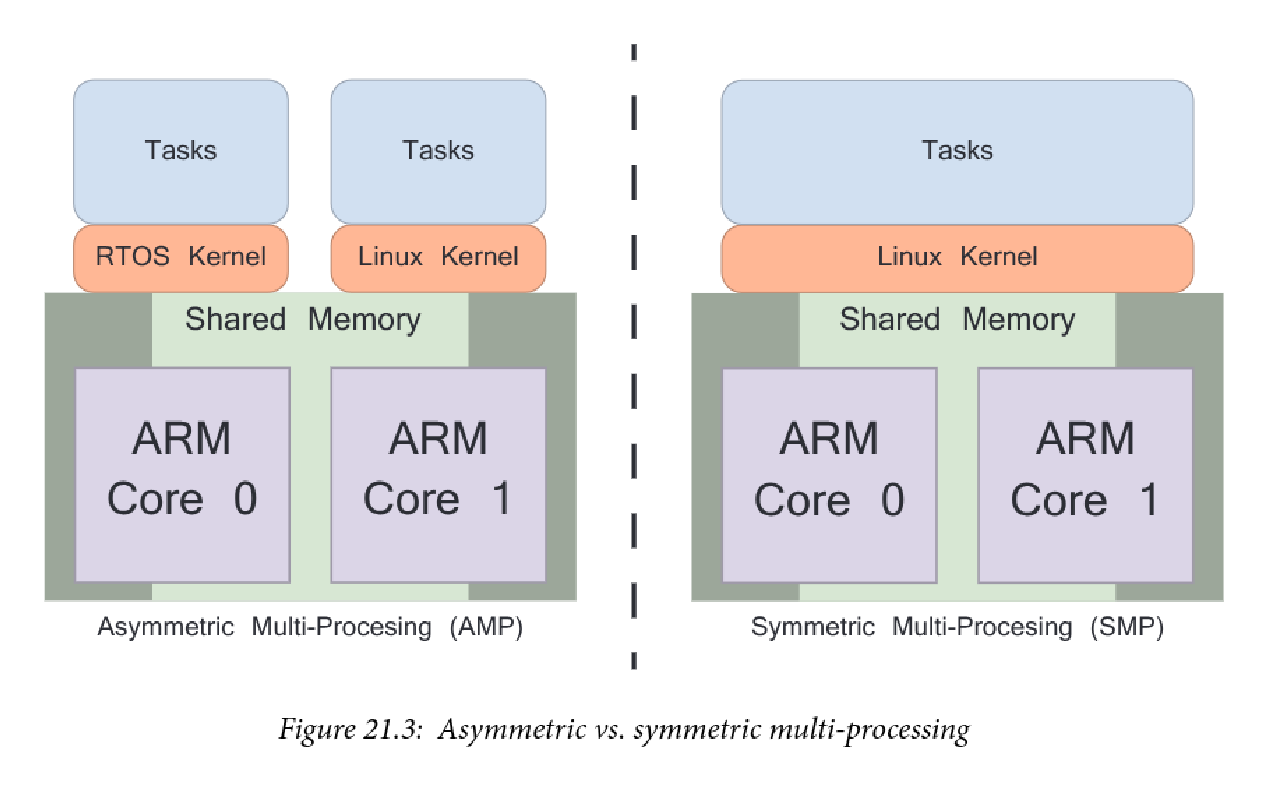
\includegraphics{cap10_amp_smp}
\caption[Procesamiento AMP y SMP]{%
Comparación de procesado AMP vs.\ SMP para el mismo procesador ARM de 2 \emph{cores}.
Extraído de~\cite{Crockett2014}.\label{f:sw-amp-smp}}
\end{figure}

La primera es cómo vamos a utilizar los diferentes \emph{cores} presentes, y tenemos
varias opciones: en la Fig.~\ref{f:sw-espectro-smp-amp} se presentan ejemplos
de sistemas operativos y su posición en el espectro.

\begin{figure}[H]
\centering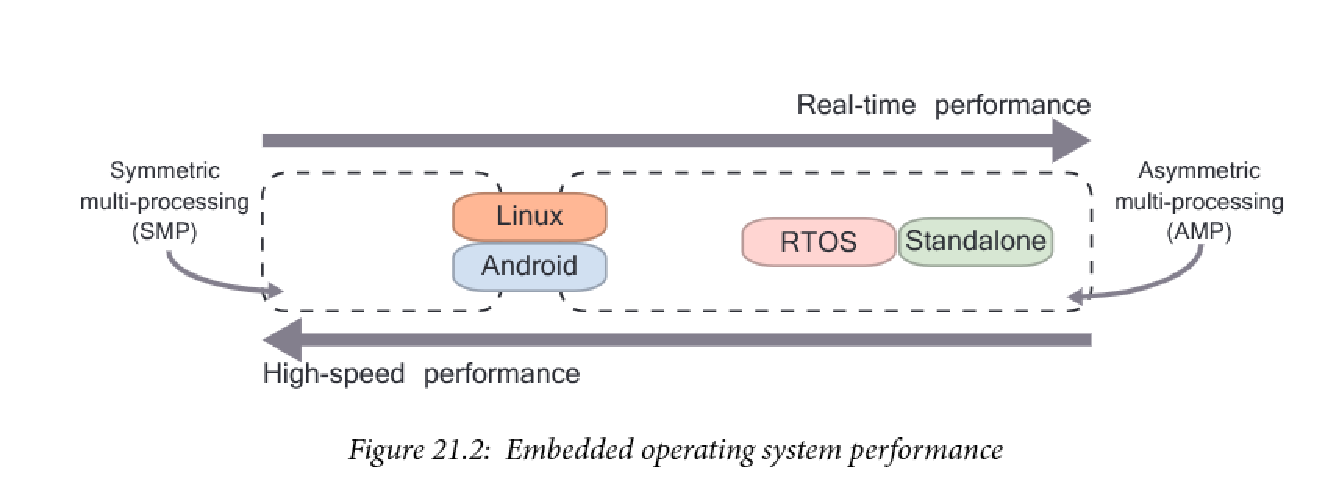
\includegraphics{cap10_espectro_smp_amp}
\caption[Ejemplos de OS en el espectro SMP-AMP]{%
Ejemplos de OS y posición en el espectro SMP-AMP. Standalone representa el
punto más extremo en \emph{real-time}; RTOS es un SO orientado a aplicaciones
\emph{real-time}.\label{f:sw-espectro-smp-amp}}
\end{figure}

\subsection{Elección del sistema operativo}
\label{S:sw-eleccion-os}

La más importante es nuestro requerimiento en tiempo de respuesta del OS, en
particular la \textbf{latencia de acceso en el peor caso}. Esto es esencial para
aplicaciones que requieren tiempos de respuesta mínimos, como accionadores
mecánicos. Las opciones principales de sistemas operativos se presentan en la
Tabla~\ref{t:sw-alternativas-os}.

\begin{table}[H]
\centering
\caption[Comparación de OS posibles en latencia]{%
Tabla comparativa de OS posibles en latencia.\label{t:sw-alternativas-os}}
\small
\begin{tabularx}{\textwidth}{|>{\raggedright\arraybackslash}p{0.17\textwidth}%
  |>{\raggedright\arraybackslash}p{0.15\textwidth}%
  |>{\raggedright\arraybackslash}X|>{\raggedright\arraybackslash}X%
  |>{\raggedright\arraybackslash}p{0.14\textwidth}|}
\hline \encabezado \textbf{Opción} & \textbf{Configura\-ción típica en Zynq} &
  \textbf{Latencia de peor caso} & \textbf{Qué provee} &
  \textbf{Costo de desarrollo} \\ \hline
\textbf{Standalone} (\emph{bare-metal}) & un núcleo, o AMP & determinística: no
  hay nada entre el programa y el hardware & \emph{drivers} básicos de Xilinx (BSP); no
  hay red, archivos ni procesos & alto: todo se escribe a mano, en C \\ \hline
\textbf{FreeRTOS} & AMP & acotada y garantizada por diseño & \emph{scheduler}
  por prioridades, colas, semáforos; red y sistema de archivos como bibliotecas
  aparte & medio-alto \\ \hline
\textbf{Linux de propósito general} & SMP & sin cota & procesos, memoria
  virtual, red, sistema de archivos, Python, ssh & bajo \\ \hline
\end{tabularx}
\end{table}

Todos los requerimientos sensibles en latencia se transfirieron al PL, así que
la opción de \emph{high-speed performance} es más que ideal como punto de
partida. En nuestro caso utilizamos el sistema operativo desarrollado por el
equipo de Pitaya. Esto no es del todo un requerimiento obligatorio, pero nos
provee un conjunto de facilidades realmente considerables, con modificaciones al
\emph{kernel mainline} (este es el base) y con adiciones sobre la capa de
usuario.

\subsection{Facilidades del Linux}
\label{S:sw-facilidades-linux}

Los servicios más importantes del mismo se presentan en la
Fig.~\ref{f:sw-kernel-linux}; estos incluyen el manejo de la memoria virtual, la
estructura de procesos (flujo de ejecución) y el \emph{scheduler}, y los \emph{drivers}
de IO de red y de memoria primaria y secundaria.

\begin{figure}[H]
\centering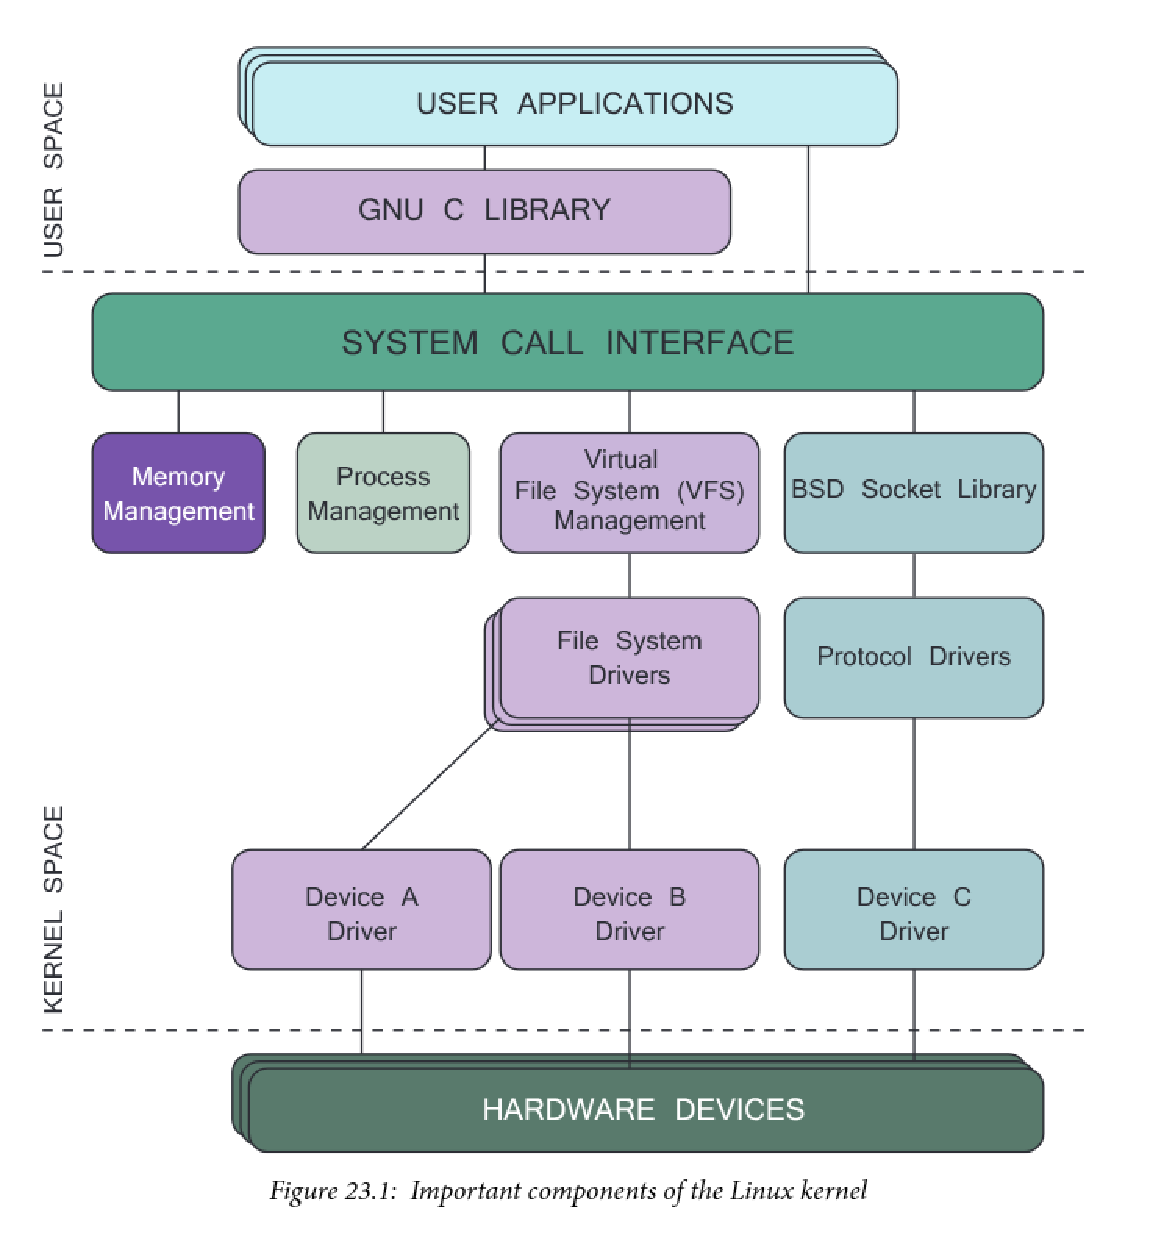
\includegraphics{cap10_kernel_linux}
\caption[Componentes del \emph{kernel} de Linux]{%
Listado de componentes del \emph{kernel} de Linux.\label{f:sw-kernel-linux}}
\end{figure}

El \textbf{\emph{kernel}} de Linux es el código del sistema operativo: esto incluye el
conjunto de estructuras internas y las APIs definidas para el manejo del mismo,
y no necesariamente incluye los \emph{drivers} particulares del HW presente. Pero al
compilar el sistema operativo (es un programa en C compilable como cualquier
otro) todos estos elementos se traducen en código máquina para el \emph{host} deseado.

\subsection{Funcionalidades de software presente}
\label{S:sw-funcionalidades}

En la Tabla~\ref{t:sw-facilidades} se presentan las funcionalidades presentes y
utilizadas en este proyecto. Estas son extremadamente útiles porque ya plantean
la base de cómo manejar el SW desde la capa de usuario, mucho más fácil para el
desarrollo acelerado. Es más, los primeros seis meses de trabajo con este
proyecto se estuvo trabajando con la modificación de un \emph{bootloader} para el
proyecto de Pavel Demin, que utiliza una distribución del tipo Alpine,
especializada para embebidos. Todo ese esfuerzo fue infructuoso, pero nos enseñó
lo importante que es tener estas funcionalidades elementales funcionando de
forma correcta para comenzar un desarrollo mínimo.

\begin{table}[H]
\centering
\caption[Facilidades del SW que provee la distribución de Pitaya]{%
Tabla de facilidades del SW que provee la distribución de Pitaya de
antemano.\label{t:sw-facilidades}}
\small
\begin{tabularx}{\textwidth}{|>{\raggedright\arraybackslash}p{0.27\textwidth}%
  |>{\raggedright\arraybackslash}X|>{\raggedright\arraybackslash}p{0.15\textwidth}|}
\hline \encabezado \textbf{Facilidad} & \textbf{Beneficio} &
  \textbf{Quién la provee} \\ \hline
\textbf{\ruta{/dev/mem} + \codigo{mmap}} & acceder al PL sin escribir un \emph{driver}
  particular & \emph{kernel} (\emph{mainline}) \\ \hline
Ubuntu ARM + Python 3.10 + NumPy & un entorno de trabajo completo en la placa,
  sin compilar nada & distribución \\ \hline
\codigo{systemd}, ssh, rsync & servicios que arrancan solos y despliegue por
  red & distribución \\ \hline
\emph{Bootloader} & FSBL generado para este PS7, U-Boot, \emph{kernel} 5.15-xilinx y el
  \emph{device tree} de \textbf{esta} placa, todo armado. Es el ítem más valioso de la
  lista y el que más trabajo ahorra & \\ \hline
API de \emph{deep memory} (\codigo{rp\_AcqAxi*}) & capturar a DDR por los
  puertos HP desde la librería, sin RTL propio & \\ \hline
Las regiones de DDR ya reservadas & \codigo{buffer@1000000} (2~MB, para la
  \emph{deep memory}) y \codigo{labuf@a000000} (32~MB, del analizador lógico),
  en el \emph{device tree} de fábrica & \\ \hline
\textbf{\codigo{fpgautil}} (\ruta{/opt/redpitaya/bin/}) & programa la PL y
  aplica el \emph{overlay} de \emph{device tree} en un comando & \\ \hline
\textbf{\codigo{monitor}} (\ruta{/opt/redpitaya/bin/}) & leer/escribir un
  registro de la PL desde la \emph{shell}, y con \codigo{-f} el \textbf{modelo de placa
  grabado en la EEPROM} & \\ \hline
\textbf{\codigo{scpi-server}} (TCP 5000) & manejar la placa como un instrumento
  de banco desde MATLAB, LabVIEW o Python & \\ \hline
\end{tabularx}
\end{table}

A continuación describimos algunos errores encontrados a nivel de HW
(especialmente en el proyecto de Pitaya) y cómo los evitamos.

\subsection{Modos de fallo en el HW implementado}
\label{S:sw-modos-fallo}

Todo el software trabaja dentro del espacio de usuario: no escribimos un \emph{driver}
propio, sino que hacemos uso del \emph{device} \ruta{/dev/mem}, que representa la
memoria física, dentro del espacio de direcciones del proceso.
\begin{enumerate}
  \item \textbf{Lecturas masivas}: no se limita el tipo de operaciones que puede
    hacer el PS sobre la región de memoria del PL; en especial, el modelo de
    memoria \emph{Device} únicamente habla del reordenamiento y de las propiedades de
    cacheo. No se impide que el compilador emita instrucciones de acceso
    múltiple (\codigo{LDM}/\codigo{STM}) o de NEON. Muchos de los \emph{drivers} de
    Linux traducen estas instrucciones en transferencias de alto \emph{throughput}, con
    ráfagas o accesos anchos, las cuales nuestro \emph{slave} en el PL no acepta. Este
    rechazo es un tipo de bus \emph{fault} presentado internamente con un código de
    \emph{external abort}, escalando hasta un error fatal que \textbf{reinicia
    el sistema}.
\end{enumerate}

La existencia de estos modos de fallo según la utilización del usuario es lo que
impulsa la creación de un \emph{driver} en el espacio del \emph{kernel}. Esto no es más que
seguir la API del sistema operativo en cuestión; nosotros vamos a implementar
una API propia en el espacio de usuario que evita los modos de falla
identificados.

%==============================================================================
\section{API: \emph{Application Programming Interface}}
\label{S:sw-api}

Esta es la librería con la que podemos acceder a diversos tipos de
\textbf{registros, algoritmos y funcionalidades} en SW en el espacio de usuario
(no del \emph{kernel}). Para esta utilizamos una estructura extremadamente similar a la
que emplea el proyecto original de Pitaya. En la Fig.~\ref{f:sw-capas} se
presentan los 6 niveles de la \textbf{jerarquía de dependencias} de este
software, en el sentido de que las capas superiores utilizan las capas
inferiores. La misma consta de un \emph{driver} escrito en C++ en la capa de usuario
(capas 1--4, en color rojo), mientras que los bloques azules son
\emph{bindings} a Python.
\begin{enumerate}
  \item \textbf{Mapeo crudo}: se utiliza el dispositivo \ruta{/dev/mem} y
    \codigo{mmap} para acceder a regiones físicas.
  \item \textbf{Acceso a palabras}:
  \begin{itemize}
    \item Se definen transacciones de 32 bits (el ancho de bus presente) con las
      funciones \codigo{w32} / \codigo{r32} / \codigo{\_read\_words}, en Python
      mediante la librería \codigo{ctypes}, para las regiones de memoria
      asociadas al bus de Pitaya. Gracias a esto no tenemos el modo de falla por
      ancho de palabras explicado en la Sec.~\ref{S:sw-modos-fallo}.
    \item Para otras direcciones se pueden implementar accesos más anchos. En
      este proyecto no se lo implementó.
  \end{itemize}
  \item \textbf{\emph{Handlers}}: son clases \textbf{compartidas por todo el sistema},
    generalmente del tipo \emph{singleton}. Debido a que son compartidas por todo el
    sistema, generalmente se las asocia al sistema operativo (esto sería un
    \emph{driver} en la capa de OS). Sin embargo, podemos manipularlas en el espacio de
    usuario con cualquier lenguaje de programación que deseemos: podríamos hacer
    una clase en Python equivalente para manipular el \emph{handler} descrito en
    nuestra librería en C o, mejor aún, utilizar el código fuente de la
    librería para compilar un código análogo pero en Python. Esto es lo que hace
    el \emph{binding}.
  \item \textbf{Métodos de \emph{handlers}}: adquisición y configuración.
  \begin{itemize}
    \item Implementan los bucles de adquisición presentados en los Caps.~\ref{C:implmca} y~\ref{C:osc}.
    \item El sistema devuelve el dato con un formato \textbf{conocido} en tiempo
      de ejecución.
  \end{itemize}
  \item \textbf{Código de sesión y fuentes}: guardado continuo de eventos y
    resumen.
  \begin{itemize}
    \item Abstracciones que utilizamos para agregar las fuentes y receptores de
      información presentes.
  \end{itemize}
  \item \textbf{Aplicaciones}: \emph{scripts} que utilizan cualquiera de las
    funcionalidades previas.
\end{enumerate}

\begin{figure}[H]
\centering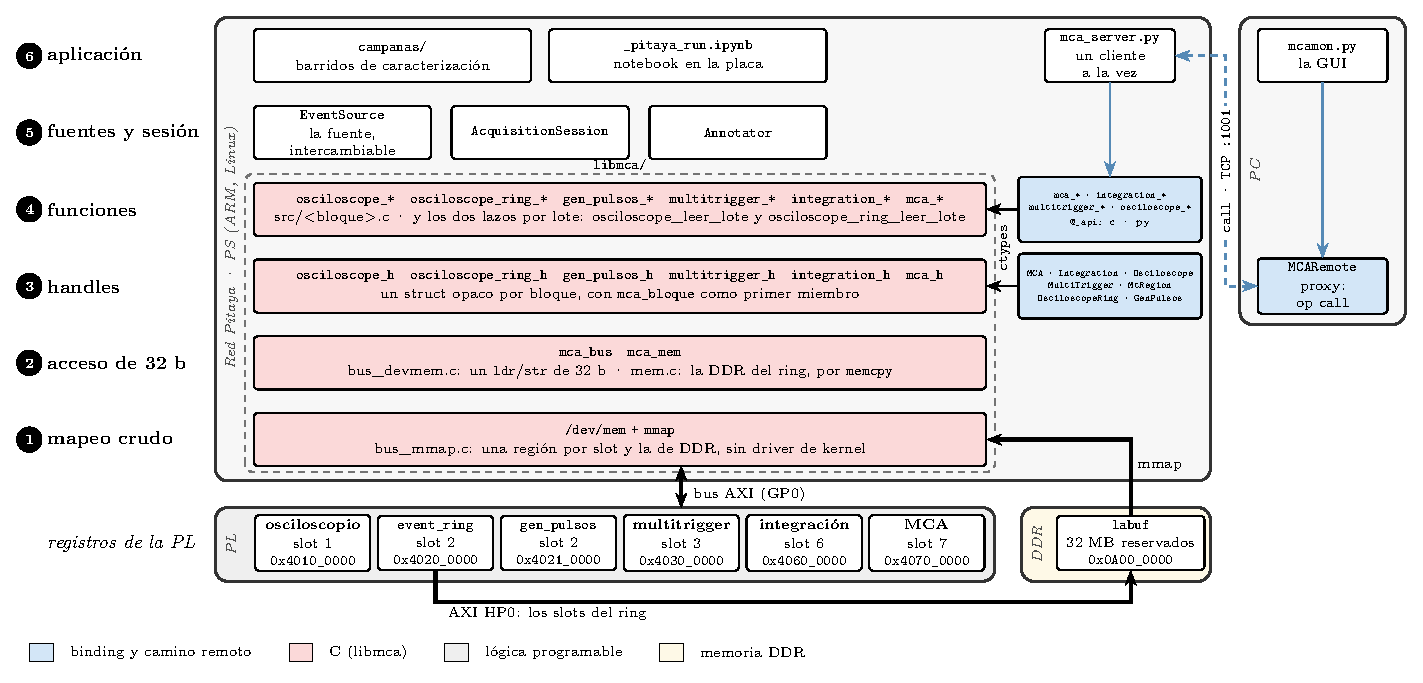
\includegraphics{cap10_niveles}
\caption[Capas de abstracción del SW]{%
Capas de abstracción de SW desarrolladas para este proyecto.\label{f:sw-capas}}
\end{figure}

Los \emph{handles} son clases del tipo \emph{singleton} porque, si no, podemos tener dos
procesos que operan sobre la misma región de memoria compartida (el rango de
direcciones de un módulo) sin un esquema de contención previamente acordado. Un
primer acercamiento podría ser configurar que la región pueda ser mapeada una
única vez. Esto no resulta beneficioso porque sería una denegación total a un
proceso, de forma que resultaría en un error en tiempo de compilación, lo cual
no es deseado. La otra es darle la capacidad de acceder a ese recurso, pero
mediante un objeto compartido y único que se encargue de implementar la
contención y el reparto del servicio: este patrón es el \emph{singleton}.

La ventaja de dividirlo por secciones en estos seis niveles es que podemos
realizar \emph{tests} para cada una de las capas individuales (\emph{unit testing}).
Para el funcionamiento correcto de la API se necesita cargado el \emph{bitstream} del
HW correcto, el que diseñamos; esto incluye la versión de los módulos
individuales y la del \emph{top} de integración. En la Sec.~\ref{S:ap-sw-bitstream}
se presentan más detalles.

%==============================================================================
\section{\emph{Driver} en C++: \texorpdfstring{\texttt{libmca}}{libmca}}
\label{S:sw-libmca}

Se llama \codigo{libmca}, pero cuenta con \emph{handlers} para todos los submódulos
instanciados dentro del módulo de integración. La idea principal consiste en
asociar cada recurso compartido a una estructura \emph{singleton} dada; por esto
planteamos:
\begin{itemize}
  \item Nivel 1, el mapeo: se abre \ruta{/dev/mem} y se mapea la región física
    de un \emph{slot} con \codigo{mmap}. El único archivo que accede a los registros
    del PL es \ruta{bus_devmem.c}, y se comprueba al compilar que no emita
    instrucciones de acceso múltiple.
  \item Nivel 2, el acceso por palabras:
  \begin{itemize}
    \item \codigo{mca\_bus}: implementa el acceso al bus \emph{custom}, asegurando el
      tipo de acceso. Tiene dos \emph{backends}: \codigo{devmem}, el real, y uno por
      \emph{callbacks}, que usan los \emph{tests} y el modelo sin placa. Operaciones
      principales:
    \begin{itemize}
      \item \codigo{mca\_bus\_open\_devmem()} mapea la subregión del \emph{slot}, y
        \codigo{mca\_bus\_close()} libera el mapeo.
      \item El acceso por palabra: \codigo{w32()}/\codigo{r32()}, y
        \codigo{read\_words()}, que lee $n$ palabras de a una, nunca como
        ráfaga.
      \item Verifica la alineación y el rango de cada acceso antes de llegar al
        \emph{backend}.
    \end{itemize}
    \item \codigo{mca\_mem}: el acceso a la región de DDR que escribe el ring.
      Es un tipo aparte porque no tiene la restricción del bus: se copia de a
      bloques, y por eso es rápido. Se mapea sin caché, porque los puertos HP no
      son coherentes con la caché.
  \end{itemize}
  \item Nivel 3, los \emph{handles}: \codigo{mca\_bloque} es la base común de todos
    ellos (el bus, si el \emph{handle} es dueño de él, y el último error), y cada
    \codigo{*\_regs.h} contiene el mapa de registros de su bloque. Al abrir un
    \emph{handle} se comprueba el \emph{magic} del bloque.
\end{itemize}

Los detalles de estas clases se presentan en la Fig.~\ref{f:sw-clases-base};
esta figura también muestra la existencia de \codigo{mca\_api.h}, que contiene
la \emph{metadata} de la versión de la API y los códigos de error de las llamadas a las
funciones. En la parte superior aparece cómo utilizar esta librería: a la
derecha, la forma estándar de C mediante un \codigo{\#include}, y a la
izquierda, la forma según el \emph{binding} de Python, que la incluye mediante un
\codigo{import}.

\begin{figure}[H]
\centering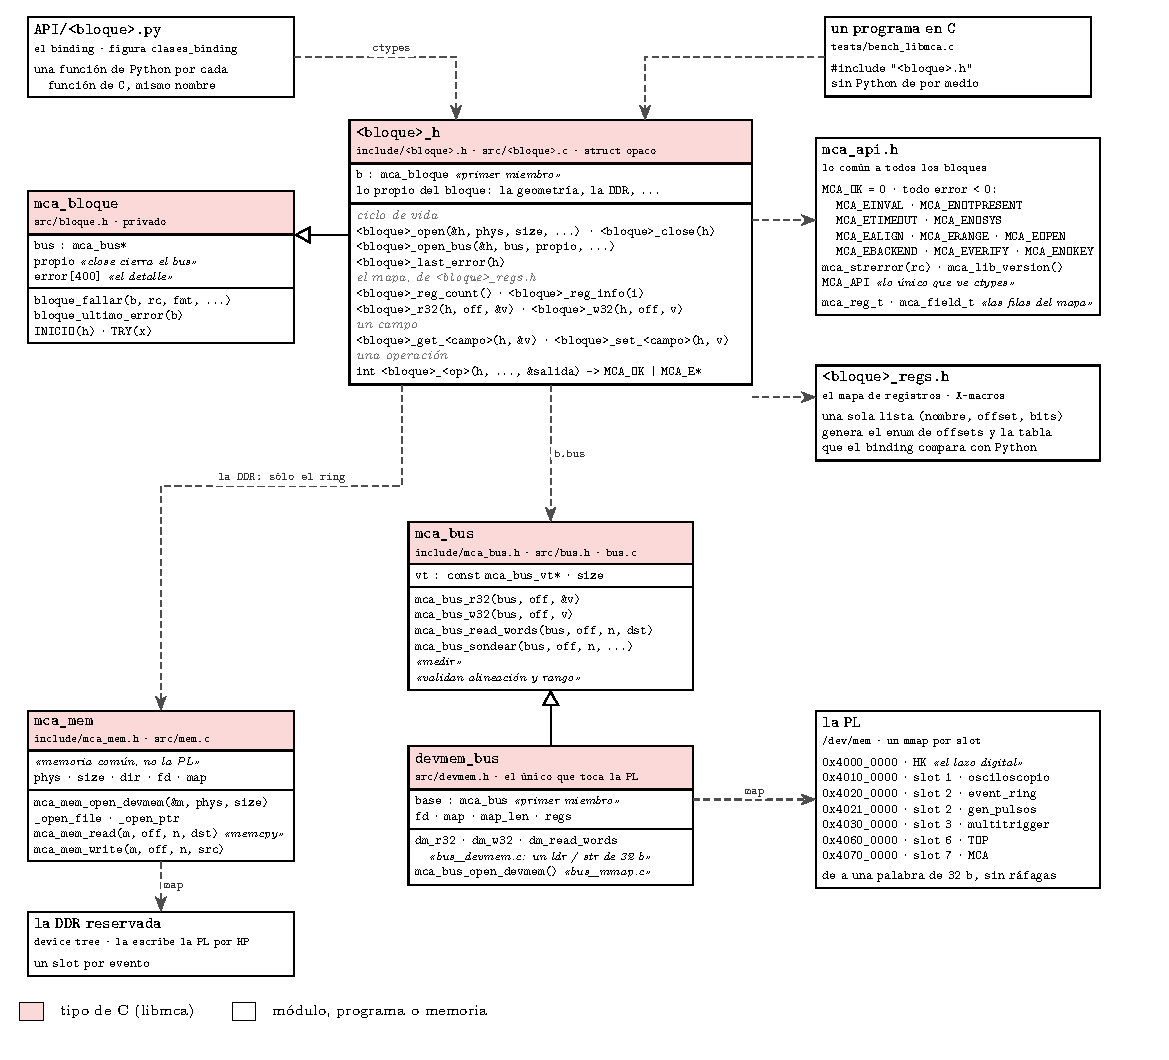
\includegraphics{cap10_clases_bloque}
\caption[Clases base de \codigo{libmca}]{%
Clases base de \codigo{libmca}. El \emph{handle} con \codigo{mca\_bus} representa el
bloque fundamental para representar los \emph{slots} de la integración\label{f:sw-clases-base}}
\end{figure}

\subsection{Bloques implementados y métodos de \emph{handlers}}
\label{S:sw-bloques}

En la Fig.~\ref{f:sw-bloques} se presentan todos los bloques definidos para este
proyecto: todos son clases derivadas de \codigo{mca\_bloque}, y se presentan los
métodos especializados para cada uno. La API implementada en este proyecto sigue
la nomenclatura \codigo{\textless módulo\textgreater\_\textless capa\textgreater\_\textless campo\textgreater} para las funciones. En la
Tabla~\ref{t:sw-api-nombres} se presentan ejemplos en cada uno de estos niveles.

\begin{figure}[H]
\centering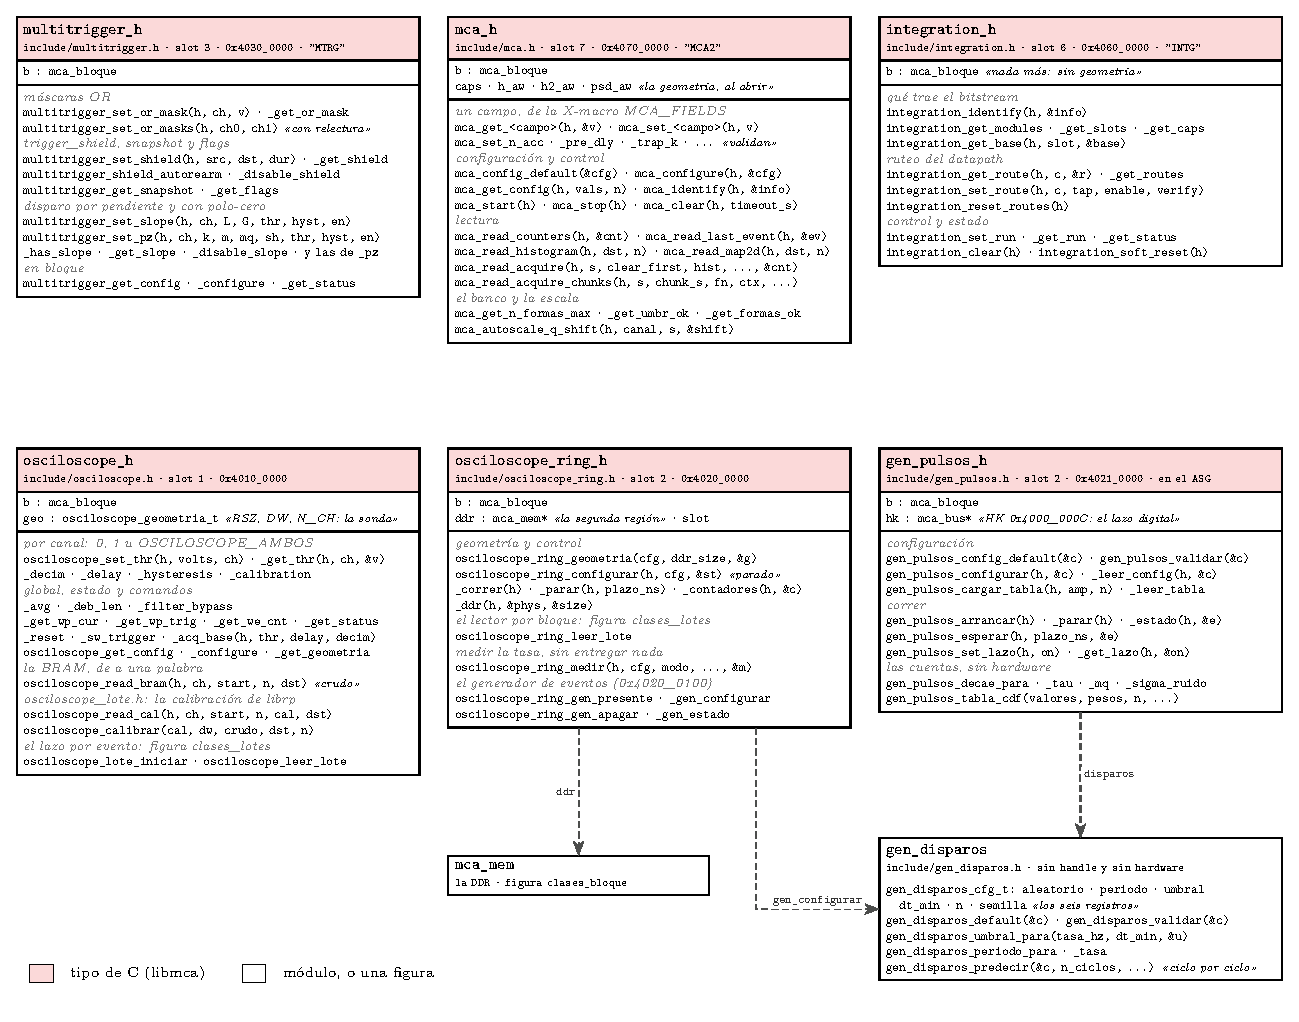
\includegraphics{cap10_clases_libmca}
\caption[Clases fundamentales de \codigo{libmca}]{%
Clases fundamentales en la librería \codigo{libmca}. Se presentan las clases
\codigo{multitrigger}, \codigo{mca}, \codigo{integracion},
\codigo{osciloscope}, \codigo{osciloscope\_ring} y
\codigo{gen\_pulsos}.\label{f:sw-bloques}}
\end{figure}

\begin{table}[H]
\centering
\caption[Estructura de nombres de la API]{%
Estructura de nombres de la API.\label{t:sw-api-nombres}}
\small
\begin{tabularx}{\textwidth}{|l|>{\raggedright\arraybackslash}p{0.3\textwidth}%
  |>{\raggedright\arraybackslash}X|}
\hline \encabezado \textbf{Capa} & \textbf{Qué dice} & \textbf{Valores}
  \\ \hline
1 $\cdot$ módulo & bloque que utiliza & \codigo{mca\_} $\cdot$
  \codigo{osciloscope\_} $\cdot$ \codigo{osciloscope\_ring\_} $\cdot$
  \codigo{multitrigger\_} \\ \hline
2 $\cdot$ tipo de API & clase de operación & cfg/\emph{status} $\cdot$
  \codigo{read\_} $\cdot$ \codigo{write\_file\_} / \codigo{save\_file\_}
  \\ \hline
3 $\cdot$ campo & el registro o la operación concreta & \codigo{thr},
  \codigo{gate\_long}, \codigo{histogram}, \ldots \\ \hline
\end{tabularx}
\end{table}

Muchos de estos elementos tienen estructuras internas, por ejemplo
\codigo{osciloscope\_lote\_t}, que no se detallan en profundidad en este
trabajo, pero se nombran en la Tabla~\ref{t:ap-sw-estructuras} de la
Sec.~\ref{S:ap-sw-estructuras}.

\subsection{Adquisición de un evento mediante la API}
\label{S:sw-adquisicion}

Tenemos un ciclo de software que \textbf{abstrae} la implementación específica
del flujo de adquisición. En el módulo osciloscopio, por ejemplo, el flujo es el
mismo con las dos interfaces de comunicación, la BRAM y el ring en DDR, aunque
cada una tiene su propio mecanismo de transferencia. La API se encarga de los
pasos que dependen de la implementación; estos se describen en la
Sec.~\ref{S:osc-flujo-basico} (BRAM), la Sec.~\ref{S:osc-uso-anillo} (ring) y
la
Sec.~\refpend{S:implmca-flujo}{Implementación del MCA: flujo de utilización del
módulo} para cada módulo.

Hay que ver qué pasa con una traza del osciloscopio después de leerla. En la
Fig.~\ref{f:sw-lazos}(a) y (b), C la escribe directamente en la fila siguiente
de un \textbf{\emph{batch}}, una estructura que se reserva una sola vez al arrancar la
corrida. No es un \emph{append}: no se copia ni se reserva memoria por evento, y
Python interviene una sola vez por \emph{batch}. Los \emph{batches} son siempre los mismos
objetos y circulan entre dos hilos: el lector, que los llena, y el escritor, que
los guarda.

\begin{figure}[H]
\centering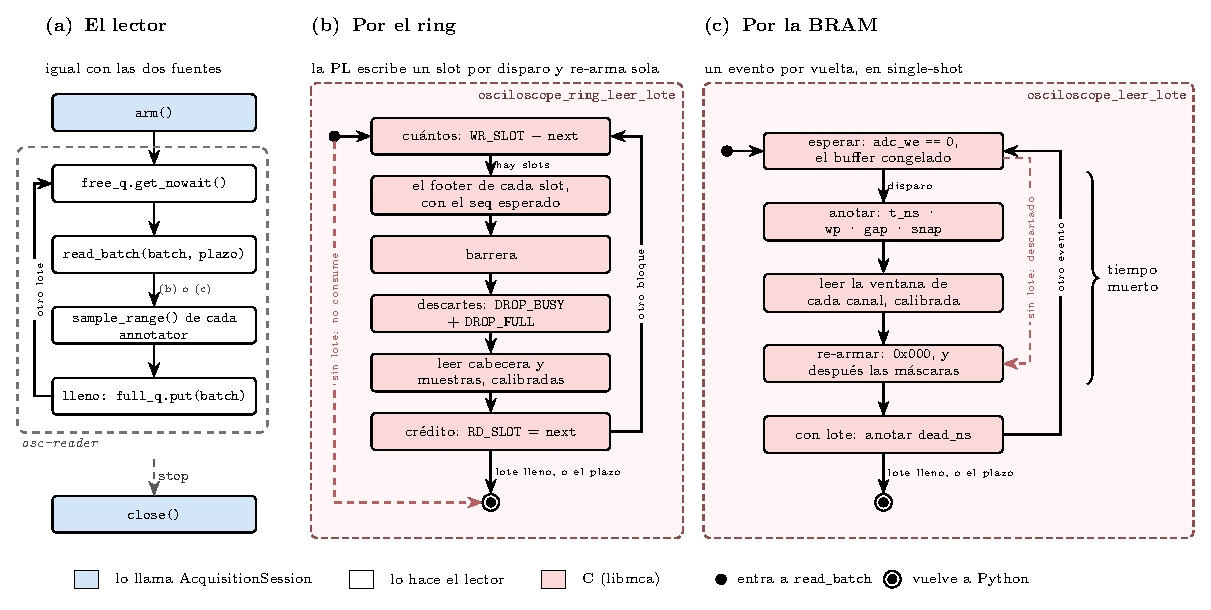
\includegraphics{cap10_maquinas_estados}
\caption[Lazos de adquisición por software]{%
Lazos de adquisición por software. (a) El osciloscopio por la BRAM: Python llama
a \codigo{arm()} una vez, a \codigo{read\_batch()} una vez por \emph{batch} y a
\codigo{close()} al final. Adentro de \codigo{read\_batch}, \codigo{libmca} lee
un evento por vuelta, en C y sin el GIL, y re-arma el osciloscopio después de
cada uno. (b) El osciloscopio por el ring: el mismo lazo de Python; adentro, un
bloque de \emph{slots} por vuelta, y nadie re-arma desde el PS.\label{f:sw-lazos}}
\end{figure}

\subsection{\emph{Binding} y clases de sesión Python}
\label{S:sw-binding}

Esta es una capa que expone cada función de C como una función de Python, con el
mismo nombre y los mismos argumentos; funciona a partir de linkear el binario
compilado \ruta{libmca.so}. Sólo traduce los tipos (enteros, structs, arreglos
de NumPy) y convierte los códigos de error de C (\codigo{MCA\_E*}) en las
excepciones habituales de Python (\codigo{ValueError}, \codigo{TimeoutError},
\codigo{KeyError}). Sobre esta se construye el software de captura de eventos
del osciloscopio. Sus clases separan qué se captura, \textbf{qué se agrega a cada
evento} y \textbf{cómo se coordina la corrida}:
\begin{enumerate}
  \item \textbf{\codigo{EventSource}, la fuente.} Define cuándo ocurre un evento
    y entrega su traza. No es una clase base sino una interfaz: sirve como
    fuente cualquier objeto con los métodos \codigo{arm()},
    \codigo{read\_batch()}, \codigo{close()} y \codigo{meta()}. Hay dos
    implementaciones:
  \begin{itemize}
    \item \codigo{BramSource} lee la ventana de cada evento de la BRAM del
      osciloscopio;
    \item \codigo{RingSource} lee los eventos que el event\_ring dejó en la DDR.
  \end{itemize}
    En las dos, el lazo que espera el disparo y lee los datos está en C, y cada
    llamada entrega un lote entero de eventos.
  \item \textbf{\codigo{Annotator}, los anotadores.} Agregan a cada evento
    columnas que no vienen de la fuente:
  \begin{itemize}
    \item Valores constantes de la corrida (\codigo{ConstantAnnotator});
    \item Mediciones lentas, como una temperatura o una posición, que un hilo
      propio lee y deja en una caché (\codigo{CachedAnnotator}).
  \end{itemize}
  \item \textbf{\codigo{AcquisitionSession}, la sesión.} Coordina una corrida
    completa:
  \begin{itemize}
    \item Arma el esquema del evento a partir de la fuente y los anotadores;
    \item Reserva un \emph{pool} de lotes (\codigo{EventBatch}) según un presupuesto de
      RAM, preasignados por el OS;
    \item Lanza dos hilos: el lector (\codigo{ReaderThread}), que llena lotes
      desde la fuente, y el escritor (\codigo{ChunkWriter}), que guarda en disco
      cada lote lleno.
  \end{itemize}
\end{enumerate}
En la Fig.~\ref{f:sw-clases-sesion} se presenta el diagrama de clases.

\begin{figure}[H]
\centering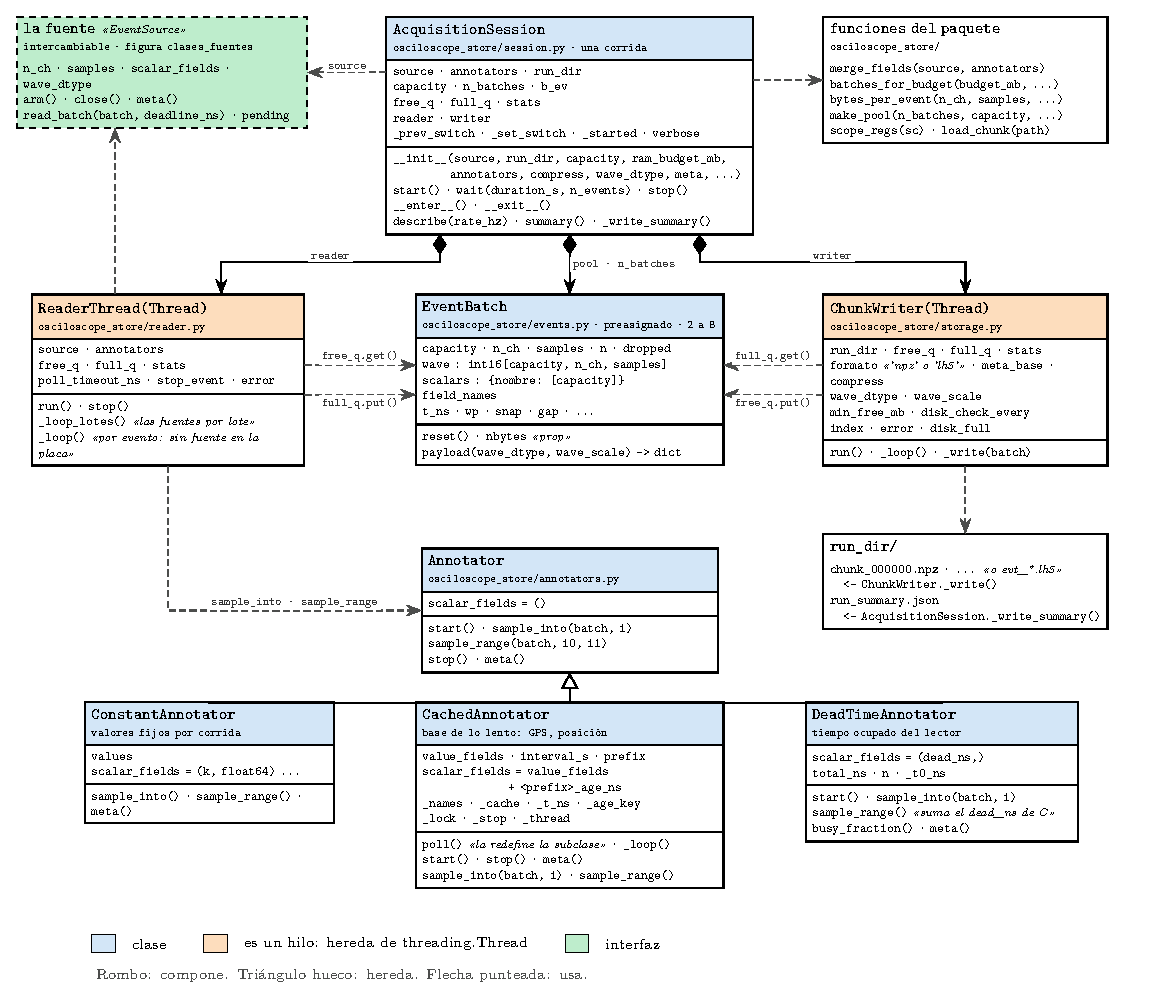
\includegraphics{cap10_clases_sesion}
\caption[Clases de sesión en Python]{%
Clases de sesión, implementadas en Python.\label{f:sw-clases-sesion}}
\end{figure}

La utilización de este \emph{binding} tiene un costo fijo por llamada, que medimos en
la Sec.~\ref{S:sw-bench-libmca}. Como el costo es por llamada y no por dato,
deja de importar cuando una llamada hace mucho trabajo. Por esto mismo decidimos
crear las clases de sesión y de manejo de archivos y eventos en Python: la
complejidad de tener todo en C no valía la pena.

%==============================================================================
\section{Guardado de archivos para el MCA y el OSC}
\label{S:sw-guardado}

Una adquisición deja dos tipos de archivos: los espectros del MCA y los eventos
del osciloscopio. En esta sección describimos qué guarda cada uno, cómo es el
archivo, cómo y dónde se escribe, y qué parte del software lo hace.

A continuación describimos los \textbf{formatos de guardado} de cada módulo.
\begin{itemize}
  \item Módulo \textbf{MCA}:
  \begin{itemize}
    \item Generalmente no necesitamos analizar la evolución del histograma con
      el tiempo: queremos su forma final. La API acumula siempre en el mismo
      histograma, y \codigo{mca\_read\_acquire\_chunks} llama a una función del
      programa cada \codigo{chunk\_s} segundos. Con eso, un programa puede
      sobrescribir el mismo archivo durante la medición o guardar los
      histogramas parciales y analizar su variación.
    \item Dada la poca cantidad de datos, el formato por defecto es
      \emph{human-readable}: un \textbf{csv} con una cabecera
      \codigo{\# clave: valor} que lleva la versión del esquema y los parámetros
      de adquisición.
    \item Implementamos además el estándar \textbf{ANSI N42.42-2011}, que abren
      otros programas de espectroscopía. Sólo admite el espectro 1D: el mapa 2D
      no entra en el formato.
    \item Hay también un \ruta{.npz} y un \ruta{.json}. \codigo{mca\_load\_file}
      lee los cuatro formatos y devuelve siempre el histograma y su \emph{metadata},
      así que el formato no cambia el análisis.
  \end{itemize}
  \item Módulo \textbf{OSC}:
  \begin{itemize}
    \item Guardamos un archivo por \emph{batch}: 4096 eventos por defecto, unos
      0.6~MB con dos canales de 32 muestras. Cada archivo se escribe con un
      nombre temporal y se renombra al terminar (\ruta{.tmp} +
      \codigo{os.replace}), así que todo archivo visible está completo. Al
      cerrar la corrida se escribe además un resumen,
      \ruta{run\_summary.json}, con los totales.
    \item Implementamos dos formatos. Uno es \textbf{LH5}, el formato basado en
      HDF5 (\emph{Hierarchical Data Format}) que usa la colaboración LEGEND
      para los datos de sus detectores de germanio~\cite{LEGENDHDF5}: lo abre
      su lector oficial sin saber nada de este proyecto, pero escribe más lento.
      El otro, el formato por defecto, es el \ruta{.npz} de
      NumPy~\cite{NumpyNEP1}: sólo necesita NumPy y es el más rápido.
  \end{itemize}
\end{itemize}

Como los sistemas de adquisición trabajan de forma independiente en HW, estos
pueden ser leídos en forma independiente. Por esto tenemos un mca-writer y un
\codigo{AcquisitionSession}. En la Tabla~\ref{t:sw-archivos} se presentan los
diferentes archivos de salida.

\begin{table}[H]
\centering
\caption[Estructura de los archivos guardados]{%
Estructura de archivos guardados.\label{t:sw-archivos}}
\small
\begin{tabularx}{\textwidth}{|>{\raggedright\arraybackslash}p{0.2\textwidth}%
  |>{\raggedright\arraybackslash}X|>{\raggedright\arraybackslash}p{0.32\textwidth}|}
\hline \encabezado \textbf{Formato} & \textbf{Estructura} & \textbf{Escritor}
  \\ \hline
\codigo{chunk\_\%06d.npz} & \codigo{wave} int16 \codigo{(eventos, canal,
  muestra)} + una columna por campo escalar + \codigo{meta} como \emph{array} 0-d &
  \codigo{ChunkWriter} \\ \hline
\codigo{evt\_\%06d.lh5} & lo mismo en LH5: una tabla \codigo{raw} con las columnas
  y una \codigo{waveform\_inN} por canal, y \codigo{meta} como texto JSON &
  \codigo{ChunkWriter} \\ \hline
\ruta{run_summary.json} & los totales de la corrida &
  \codigo{AcquisitionSession} \\ \hline
\ruta{.csv} & el espectro con la \emph{metadata} en cabecera \codigo{\#}; \textbf{el
  formato por defecto}, se abre en Excel u Origin &
  \codigo{mca\_write\_file\_histogram} \\ \hline
\ruta{.npz} / \ruta{.json} & el espectro estructurado &
  \codigo{mca\_save\_file\_*} \\ \hline
\end{tabularx}
\end{table}

Para aprovechar el formato binario del \ruta{.npz} vamos a necesitar un programa
de lectura; este está incluido en la API, con la estructura de datos deseada.

\subsection{Contenido de los archivos de trazas del osciloscopio}
\label{S:sw-contenido-trazas}

Una corrida del osciloscopio es una tabla de eventos, con la misma configuración
de principio a fin. Cada evento tiene:
\begin{itemize}
  \item \textbf{La ventana del evento}: las muestras alrededor del disparo;
  \item \textbf{Sus datos escalares}, que cambian en cada evento y declara la
    fuente: cuándo llegó (\codigo{t\_ns}), dónde estaba el puntero de escritura
    (\codigo{wp}), qué fuente disparó (\codigo{snap}) y cuántos eventos se
    descartaron antes (\codigo{gap});
  \item \textbf{Las columnas de los anotadores}: el tiempo muerto
    (\codigo{dead\_ns}), valores fijos de la corrida, o mediciones lentas, como
    una temperatura, con su antigüedad (\codigo{\textless p\textgreater\_age\_ns}).
\end{itemize}
La tabla se parte en archivos de un \emph{batch} cada uno (4096 eventos por defecto). Al
final se agrega un resumen de la corrida, \ruta{run_summary.json}.

\subsubsection{Trazas en formato \texorpdfstring{\texttt{.npz}}{.npz}}

Cada \emph{batch} lleno se guarda en un archivo \ruta{chunk_NNNNNN.npz}, numerado desde
cero. Un \ruta{.npz} es un \emph{zip} con un arreglo de NumPy (\ruta{.npy}) por
entrada, cada uno con su nombre, su forma y su tipo~\cite{NumpyNEP1}.
\codigo{np.load} lo abre como un diccionario y lee cada arreglo recién cuando se
lo pide.

Estructuramos cada \emph{batch} con tres índices, \codigo{(evento, canal, muestra)},
más una columna 1D por cada metadato. El primer eje, \codigo{capacity}, es la
cantidad de eventos que entran en un \emph{batch}; \codigo{n\_ch} es la cantidad de
canales que se adquieren en paralelo, y \codigo{samples}, la muestra dentro de
la ventana. Las muestras se guardan como \codigo{int16}: son cuentas de un ADC
de 14 bits, y en \codigo{float32} ocuparían el doble. Las columnas no son fijas:
la fuente y cada annotator declaran las suyas, y el \emph{batch} se arma al arrancar la
corrida. Este esquema se presenta en la Fig.~\ref{f:sw-esquema-evento}. El
\codigo{gap} es un \codigo{uint8} y satura en 255; por eso la cuenta exacta de
descartes va en la \emph{metadata} de cada archivo. Los descartes del final de la
corrida no tienen un evento siguiente donde anotarse, así que van en
\ruta{run_summary.json}.

\begin{figure}[H]
\centering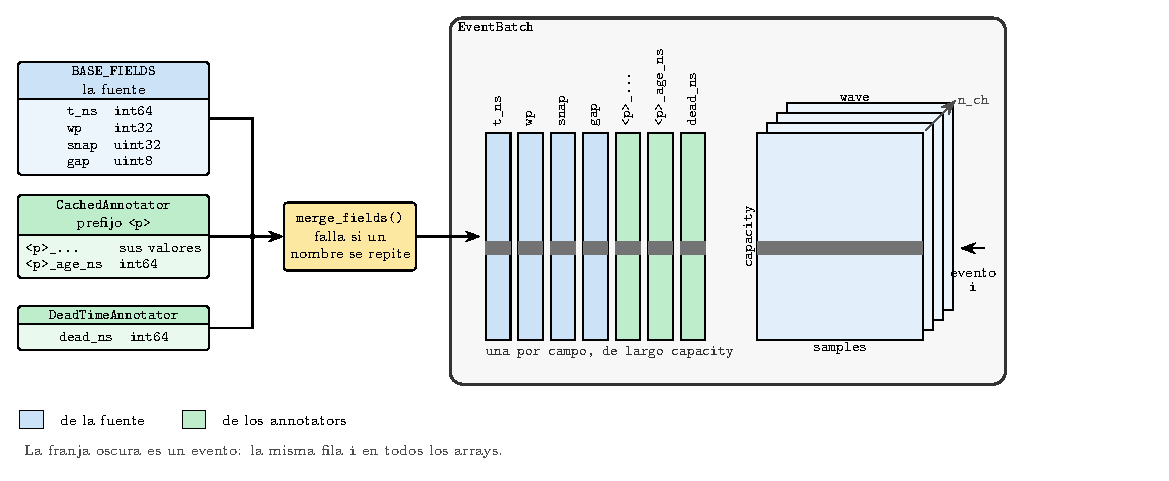
\includegraphics{cap10_esquema_evento}
\caption[Estructura de un \emph{batch} de eventos]{%
Estructura de un \emph{batch} de eventos. Es la base del guardado
automático.\label{f:sw-esquema-evento}}
\end{figure}

El formato no está hardcodeado: se puede construir en \emph{runtime} y se pueden
obtener sus campos inspeccionando \codigo{meta['schema\_version']} y
\codigo{meta['fields']}.

\subsubsection{Metodología de escritura}

El escritor guarda cada \emph{batch} apenas se llena, sin esperar a juntar varios. Para
que nunca quede a la vista un archivo a medias, primero escribe un temporal
(\ruta{chunk_000123.npz.tmp}) en la misma carpeta, y al terminar le da el nombre
final con \codigo{os.replace} (Fig.~\ref{f:sw-escritura}). Ese renombre es
atómico~\cite{Kerrisk2010} porque los dos nombres están en el mismo sistema de
archivos: otro programa ve el archivo completo o no lo ve. Por eso se puede
copiar o analizar una corrida mientras anda, y \codigo{archivos\_de\_corrida}
nunca devuelve un \ruta{.tmp}. Mientras tanto, \codigo{write()} vuelve cuando los
datos están en el page \emph{cache} del \emph{kernel}, es decir en RAM; el \emph{kernel} los pasa a la
tarjeta después. El escritor no fuerza ese paso con \codigo{fsync}. La garantía
es entonces que ningún archivo visible está incompleto, no que sobreviva a un
corte de luz~\cite{Pillai2014}. Cada 8 archivos, el escritor revisa el lugar
libre. Si quedan menos de 200~MB, para, y la sesión corta la corrida con el
motivo \codigo{disk}.

La Fig.~\ref{f:sw-escritura} muestra la secuencia: cada \emph{batch} pasa por un
\ruta{.tmp} antes de tener su nombre final, y al cerrar la corrida
\ruta{run_summary.json} sigue el mismo camino.

\begin{figure}[H]
\centering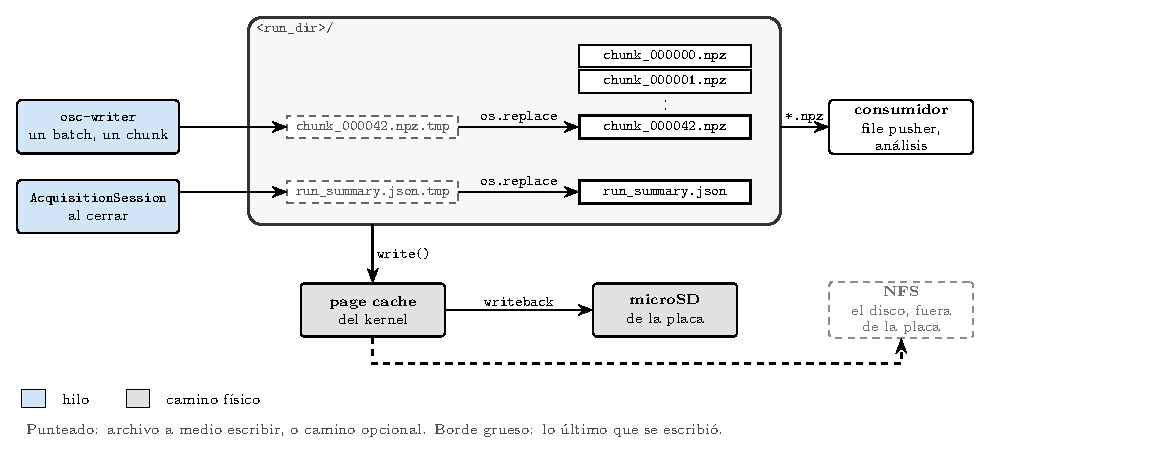
\includegraphics{cap10_escritura_corrida}
\caption[Guardado por \emph{chunks} \texttt{.npz} y resumen \texttt{.json}]{%
Metodología de guardado por \emph{chunks} \ruta{.npz} y resumen
\ruta{.json}.\label{f:sw-escritura}}
\end{figure}

\subsubsection{Localización de guardado}
\label{S:sw-localizacion}

La microSD de la placa tiene 32~GB, pero la partición del sistema tiene 6.6~GB y
quedan unos 1.4~GB libres. Más que el tamaño, limita la velocidad. La escritura
sostenida tiene un techo que no depende de la tarjeta: el controlador SD del
Zynq trabaja en modo de 4 bits con un reloj de \qty{50}{\mega\hertz}, así que el
bus llega a unos 25~MB/s. Lo que llega a la tarjeta en esta placa se presenta en
la Sec.~\ref{S:sw-bench-disco}. Para el MCA alcanza de sobra, porque un espectro
de 8192 canales ocupa 32~kB. Para el osciloscopio depende de la ventana:
\begin{itemize}
  \item \textbf{2 canales $\times$ 32 muestras} (la ventana por defecto): un
    evento ocupa 146~B. A 50~kev/s son 7.3~MB/s, por debajo de ese techo.
  \item \textbf{2 canales $\times$ 1024 muestras}: un evento ocupa 4~KiB. A
    50~kev/s son 205~MB/s, ocho veces el techo del bus. Los 1.4~GB libres se
    llenarían en \qty{7}{\second}.
\end{itemize}
La alternativa es \textbf{escribir por la red}, en un sistema de archivos NFS
montado en la placa. Para la sesión no cambia nada: \codigo{run\_dir} es
simplemente otra carpeta. Es una solución probada que no hay que implementar.

Aunque no lo parezca, la red Gigabit puede ser más rápida que la SD. Igual,
ninguno de los dos caminos alcanza para ventanas de 1024 muestras a 50~kev/s, que
piden 205~MB/s: para eso habría que acortar la ventana o bajar la tasa.

\subsubsection{\emph{Script} de guardado de trazas de datos}

Un \emph{script} de captura continua tiene que instanciar, inicializar y orquestar la
llamada de los métodos. Este programa es el que maneja la sesión de captura. En
la Fig.~\ref{f:sw-hilos} se presentan tres. El primero maneja la captura y el
guardado de las trazas del osciloscopio, el segundo maneja la captura, el
guardado y el acceso por red del MCA, mientras que el tercero se encarga de
manejar la GUI en el cliente con la librería Qt. En la
Tabla~\ref{t:sw-hilos} se presentan los hilos y sus tareas principales.

\begin{figure}[H]
\centering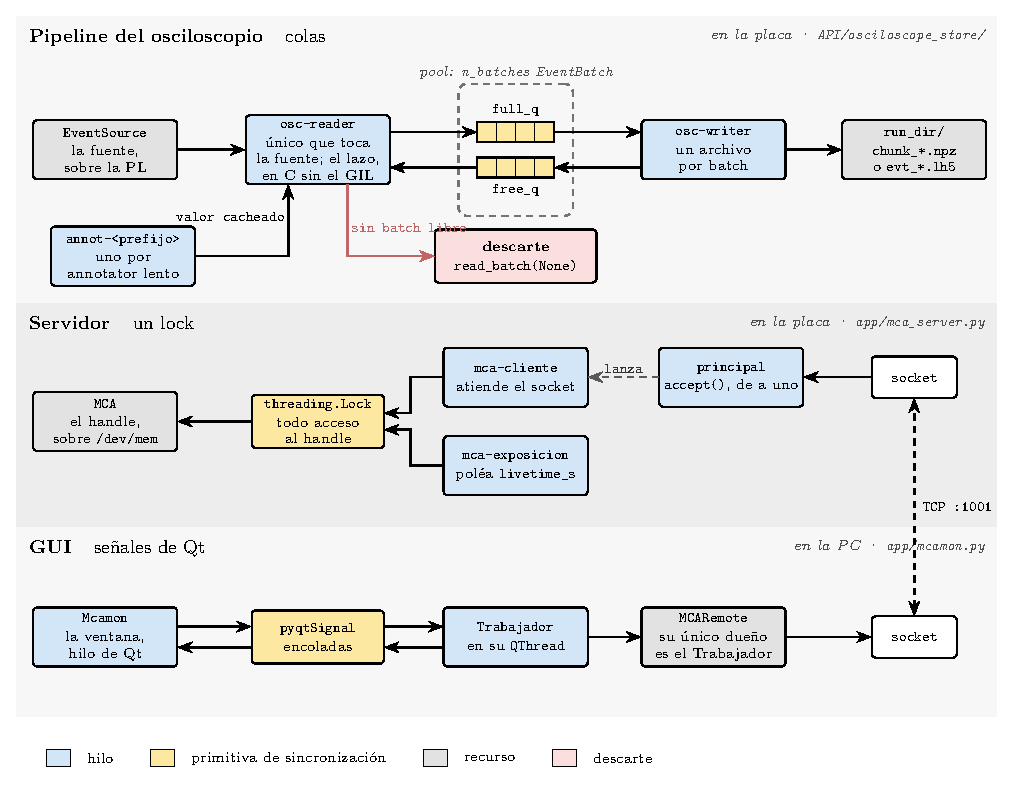
\includegraphics{cap10_hilos}
\caption[Las tres sesiones locales del programa]{%
Las tres sesiones locales de nuestro programa.\label{f:sw-hilos}}
\end{figure}

\begin{table}[H]
\centering
\caption[Hilos de captura y sus tareas]{%
Hilos de captura presentes en este proyecto y sus tareas
asociadas.\label{t:sw-hilos}}
\small
\begin{tabularx}{\textwidth}{|>{\raggedright\arraybackslash}p{0.19\textwidth}%
  |>{\raggedright\arraybackslash}p{0.22\textwidth}%
  |>{\raggedright\arraybackslash}X|}
\hline \encabezado \textbf{Hilo} & \textbf{Clase} & \textbf{Tareas} \\ \hline
principal & \codigo{AcquisitionSession} & arranca y detiene la adquisición;
  sólo espera (\codigo{wait}) y lee los contadores \\ \hline
\codigo{osc-reader} & \codigo{ReaderThread} & toma un \emph{batch} de
  \codigo{free\_q}, lo llena con \codigo{read\_batch}, les pide sus columnas a
  los anotadores y lo pasa a \codigo{full\_q} \\ \hline
\codigo{osc-writer} & \codigo{ChunkWriter} & toma un \emph{batch} de
  \codigo{full\_q}, lo guarda en un archivo y lo devuelve a \codigo{free\_q}
  \\ \hline
uno por anotador lento & \codigo{CachedAnnotator} & lee su sensor cada
  \codigo{interval\_s} y deja el valor en una caché \\ \hline
\end{tabularx}
\end{table}

El \codigo{osc-reader} no sabe de dónde vienen los eventos: lee de la fuente que
le den, \codigo{BramSource} o \codigo{RingSource}, y llena \emph{batches} de la clase
\codigo{EventBatch}. Cuando un \emph{batch} se llena (4096 eventos por defecto), lo
pasa a \codigo{full\_q}. El \codigo{osc-writer} guarda cada \emph{batch} que recibe,
así que queda un archivo por \emph{batch}: no hay un umbral de tamaño para escribir.

Los \emph{batches} son siempre los mismos objetos y circulan entre los dos hilos
(Fig.~\ref{f:sw-pool}). Al armar la sesión se crean entre 2 y 8, según el
presupuesto de RAM (\codigo{ram\_budget\_mb}, 64~MB por defecto), y después dan
la vuelta:
\begin{enumerate}
  \item \codigo{free\_q} le entrega uno al lector, que lo llena;
  \item El lector lo pone en \codigo{full\_q};
  \item El escritor lo toma y lo guarda;
  \item El escritor lo devuelve a \codigo{free\_q}.
\end{enumerate}
Es el esquema de productor y consumidor con un \emph{buffer}
acotado~\cite{Dijkstra1965}: \codigo{free\_q} y \codigo{full\_q} cuentan los
lugares vacíos y los llenos. Con los valores por defecto son 8 \emph{batches}, unos
5~MB en total. Los \emph{batches} llenos que esperan en \codigo{full\_q} son el margen
del escritor: a 10~kev/s puede atrasarse unos \qty{3}{\second} sin perder nada.
Si se atrasa más, \codigo{free\_q} se vacía y el lector descarta.

\begin{figure}[H]
\centering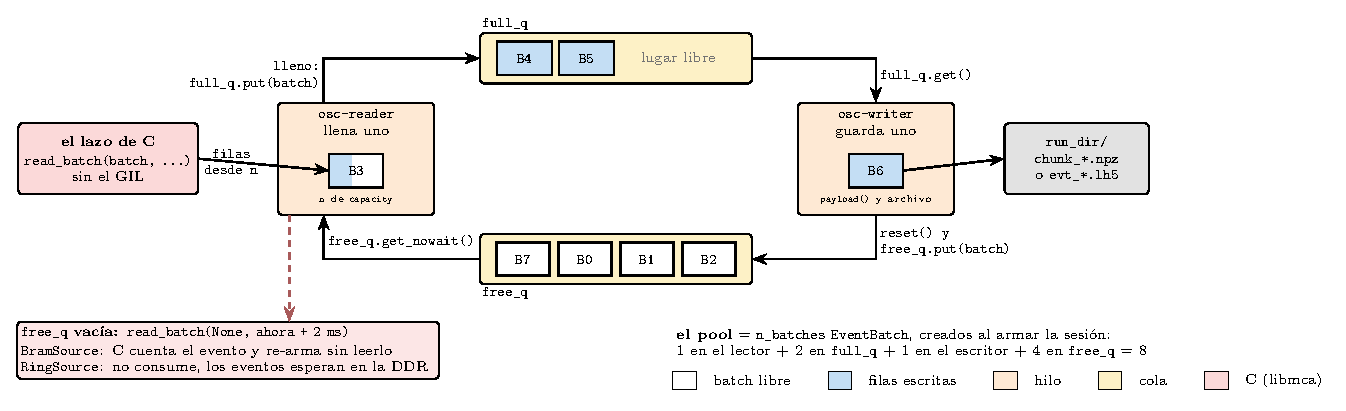
\includegraphics{cap10_pool_batches}
\caption[Cola de \codigo{EventBatch}]{%
Representación de la cola de \codigo{EventBatch}.\label{f:sw-pool}}
\end{figure}

En la Sec.~\ref{S:sw-flujo-sesion} describimos con más detalle cómo se inicia este sistema
mediante la utilización de la clase \codigo{AcquisitionSession}.

\subsubsection{Flujo de sesión de adquisición}
\label{S:sw-flujo-sesion}

En la Fig.~\ref{f:sw-flujo-sesion} se presenta el flujo de la sesión. Al
construirse, \codigo{AcquisitionSession} no toca el hardware ni lanza hilos:
arma el esquema del evento, crea los \emph{batches} del \emph{pool} y los pone en
\codigo{free\_q}. Para arrancar la medición (\codigo{start()}) sigue estos
pasos:
\begin{enumerate}
  \item Baja a \qty{1}{\milli\second} el intervalo de cambio del
    GIL~\cite{Beazley2010}, que por defecto es de \qty{5}{\milli\second}, para
    que el lector no espere tanto a que el escritor se lo devuelva.
  \item Arranca los anotadores. Los que leen sensores lentos lanzan su propio
    hilo.
  \item Arma la fuente (\codigo{source.arm()}): configura la PL, que queda
    esperando disparos.
  \item Arranca el hilo \codigo{osc-writer}, que queda esperando en
    \codigo{full\_q}.
  \item Arranca el hilo \codigo{osc-reader}, que empieza a llenar \emph{batches}.
\end{enumerate}

Mientras tanto, el hilo principal sólo espera (\codigo{wait()}): cada
\qty{0.2}{\second} revisa si se cumplió la duración o la cantidad de eventos, y
si se cayó un hilo o se llenó el disco.

Al finalizar (\codigo{stop()}), apaga en el orden inverso, para que no quede
ningún evento leído sin guardar:
\begin{enumerate}
  \item Con el ring, corta el estímulo con el hardware andando y espera, hasta
    \qty{5}{\second}, a que el lector se lleve lo que quedó en la DDR.
  \item Para el lector. Al salir, el lector pone en \codigo{full\_q} el \emph{batch}
    que tenía a medias y después un centinela (\codigo{None}).
  \item Espera al escritor, que guarda todo lo que hay en \codigo{full\_q} hasta
    encontrar el centinela.
  \item Para los anotadores, cierra la fuente (desarma la PL) y restaura el
    intervalo de cambio.
  \item Escribe \ruta{run_summary.json}, también con \ruta{.tmp} +
    \codigo{os.replace}.
\end{enumerate}

\begin{figure}[H]
\centering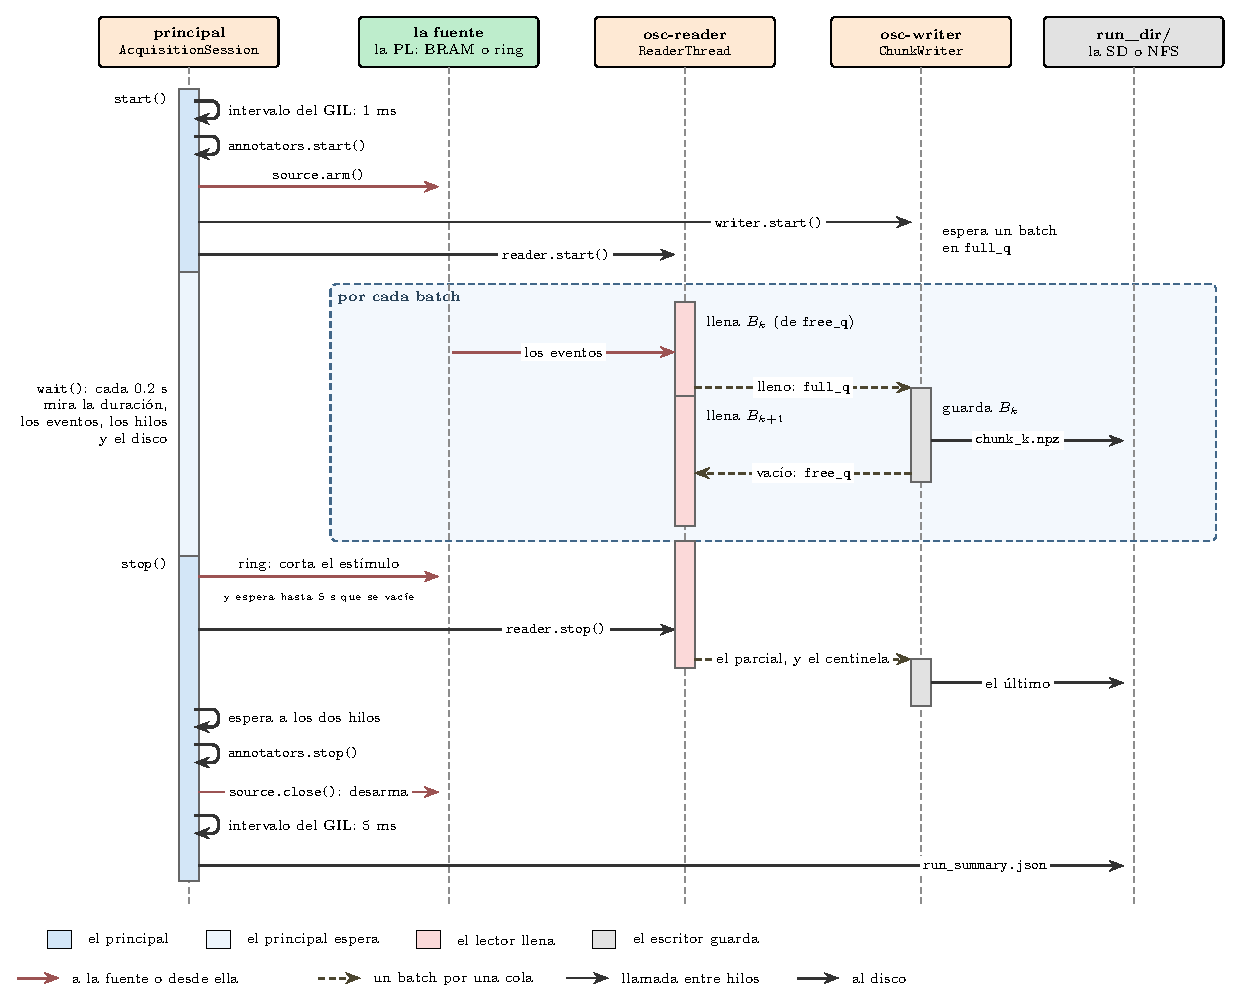
\includegraphics{cap10_flujo_sesion}
\caption[Flujo de trabajo de \codigo{AcquisitionSession}]{%
Flujo de trabajo del \codigo{AcquisitionSession}, de \codigo{start()} a
\codigo{stop()}. Por cada \emph{batch}, el lector lo llena con los eventos de la fuente
y lo pasa por \codigo{full\_q}, y el escritor lo guarda y lo devuelve por
\codigo{free\_q} mientras el lector ya llena el siguiente. Lo que pasa adentro de
cada hilo se presenta en la Fig.~\ref{f:ap-sw-hilos-captura}.\label{f:sw-flujo-sesion}}
\end{figure}

%==============================================================================
\section{Protocolo de red}
\label{S:sw-protocolo-red}

En el nivel de aplicación el sistema se comunica mediante mensajes \textbf{JSON
UTF-8 terminados en \codigo{\textbackslash n}}, seguidos opcionalmente de
\codigo{nbytes} crudos, en la Fig.~\ref{f:sw-trama}.

\begin{figure}[H]
\centering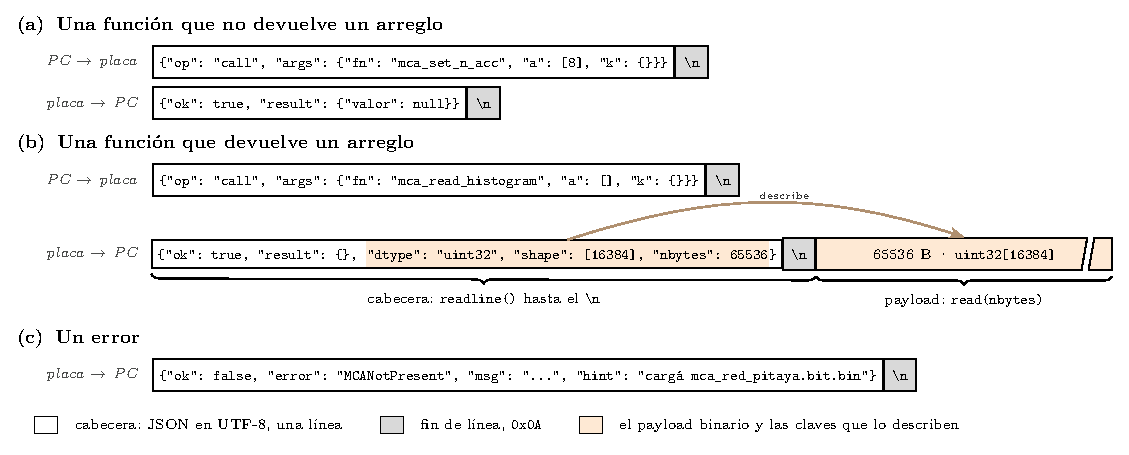
\includegraphics{cap10_trama}
\caption[Tramas del protocolo de red]{%
Ejemplos de tramas del protocolo de red: una cabecera JSON en una línea que
termina en \codigo{\textbackslash n} y el \emph{payload} binario que la cabecera
describe con \codigo{nbytes}, \codigo{dtype} y \codigo{shape}.
\label{f:sw-trama}}
\end{figure}

El flujo a nivel \emph{socket} está pensado para TCP: se creó una clase
\codigo{Channel} que tiene como objetivo serializar/deserializar la trama según
el protocolo. En la Fig.~\ref{f:sw-trama-flujo} se muestra la serialización
empleada en esta clase: mediante \codigo{readline()} obtiene fragmentos del
mensaje y mediante los \codigo{\textbackslash n} segmenta el mensaje.

\begin{figure}[H]
\centering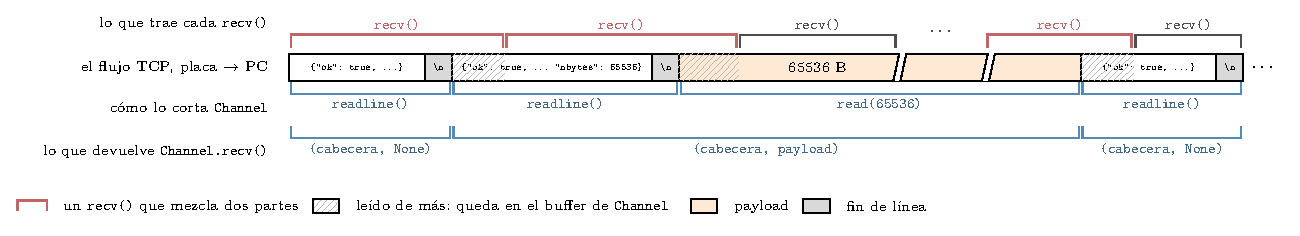
\includegraphics{cap10_trama_flujo}
\caption[Serialización de la trama en la clase \codigo{Channel}]{%
Serialización de trama JSON mediante la clase \codigo{Channel} empleando
\codigo{\textbackslash n}.\label{f:sw-trama-flujo}}
\end{figure}

\subsection{Modo de exportación de datos del ring}
\label{S:sw-exportacion-ring}

Los eventos del ring pueden llegar a un archivo por dos caminos, que se eligen
con el argumento \codigo{destino} de \codigo{ring.iniciar}. El primero es el de
la Sec.~\ref{S:sw-localizacion}: la sesión corre en la placa y escribe en una
dirección \codigo{run\_dir}, que puede estar en la microSD o en un disco de la
PC montado por NFS. Con NFS el archivo cruza la red, pero \textbf{lo sigue
armando la placa}. Eso resuelve la capacidad y la velocidad sostenida de la SD,
que limitan en corridas largas o con ventanas grandes, pero no saca del camino a
la sesión de Python en el procesador de la placa, que con ventanas cortas
también limita la tasa (Sec.~\ref{S:osc-ring-funcionamiento}).

El segundo, el modo de exportación por red, saca a la sesión del camino de los
datos en la placa (Fig.~\ref{f:sw-escritura-red}). No hizo falta una fuente
nueva: en este modo la placa no corre la sesión.

\begin{figure}[H]
\centering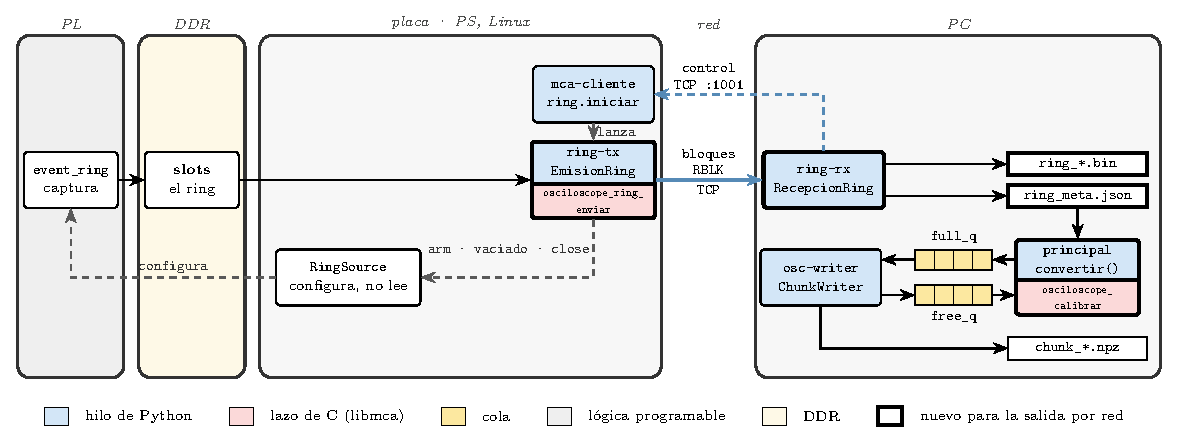
\includegraphics{cap10_escritura_archivos_por_red}
\caption[Escritura de los eventos del ring a archivos por red]{%
La escritura de los eventos del ring a archivos por red. En la placa no corre la
sesión: el hilo \codigo{ring-tx} llama a \codigo{osciloscope\_ring\_enviar}, que
copia los \emph{slots} y los manda en bloques \codigo{RBLK} por un \emph{socket} de datos, y
\codigo{RingSource} sólo configura el ring y el estímulo. En la PC,
\codigo{ring-rx} guarda el \emph{stream} tal cual en \ruta{ring_*.bin}, y
\codigo{convertir()} lo pasa a los mismos \ruta{chunk_*.npz} con el \emph{pool} y el
\codigo{ChunkWriter} de la sesión. El control va por el \emph{socket} del servidor (TCP
:1001).\label{f:sw-escritura-red}}
\end{figure}

Los datos y el control viajan por dos conexiones TCP distintas. El control usa
el \emph{socket} del servidor (TCP :1001) y el protocolo JSON de la
Sec.~\ref{S:sw-protocolo-red}. Después, la PC se conecta a ese puerto y recibe
un \emph{stream} de bloques con un formato propio. Cada bloque tiene una cabecera de
40~B (Tabla~\ref{t:sw-rblk}) y, detrás, \codigo{n} \emph{slots} tal como están en la
DDR: la cabecera del \emph{slot} (32~B) y las muestras int16 de los dos canales,
intercaladas y sin calibrar.

\begin{table}[H]
\centering
\caption[Cabecera de un bloque del \emph{stream} de datos]{%
Cabecera de un bloque del \emph{stream} de datos, en
\emph{little-endian}.\label{t:sw-rblk}}
\small
\begin{tabularx}{\textwidth}{|>{\raggedright\arraybackslash}p{0.3\textwidth}%
  |>{\raggedright\arraybackslash}p{0.2\textwidth}%
  |>{\raggedright\arraybackslash}X|}
\hline \encabezado \textbf{Campo} & \textbf{Tipo} & \textbf{Contenido} \\ \hline
\codigo{magic}, \codigo{version}, \codigo{flags} & u32, u16, u16 &
  \codigo{\textquotedbl RBLK\textquotedbl}, la versión 1 y el bit FIN \\ \hline
\codigo{seq0}, \codigo{n} & u32, u32 & el \codigo{seq} del primer \emph{slot} y la
  cantidad de \emph{slots} \\ \hline
\codigo{carga}, \codigo{bytes} & u32, u32 & los bytes por \emph{slot} y los que siguen
  a la cabecera \\ \hline
\codigo{descartados} & u64 & los eventos descartados antes del primer \emph{slot} del
  bloque \\ \hline
\codigo{t\_ns} & i64 & el reloj de la placa al leer el bloque \\ \hline
\end{tabularx}
\end{table}

%==============================================================================
\section{Resultados de \emph{benchmark}}
\label{S:sw-bench}

Dividimos las mediciones en las dos secciones principales del SW: las de
\codigo{libmca} y las de guardado por sesión en Python.

\subsection{Resultados de \emph{benchmark} para \texorpdfstring{\texttt{libmca}}{libmca}}
\label{S:sw-bench-libmca}

Se midió la misma operación por tres caminos, con el resultado de la
Tabla~\ref{t:sw-bench-libmca}:
\begin{itemize}
  \item \textbf{Python sin \emph{binding}}: la referencia, que lee los registros con
    \codigo{struct.unpack\_from} sobre el mmap, sin pasar por C;
  \item \textbf{Python con \emph{binding}}: Python $\rightarrow$ \codigo{ctypes}
    $\rightarrow$ \codigo{libmca};
  \item \textbf{C puro}: la misma función de \codigo{libmca}, llamada desde un
    programa en C sin intérprete.
\end{itemize}

\begin{table}[H]
\centering
\caption[Costo de llamada de las operaciones de \codigo{libmca}]{%
Tabla comparativa de costo de llamada de operaciones.\label{t:sw-bench-libmca}}
\begin{tabular}{|l|r|r|r|}
\hline \encabezado \textbf{Operación} (\unit{\micro\second}) & \textbf{Python}
  & \textbf{\emph{binding}} & \textbf{C} \\ \hline
leer un registro (\codigo{r32}) & 10.5 & 56.8 & 1.5 \\ \hline
leer el umbral & 15.4 & 63.7 & 1.4 \\ \hline
escribir el umbral & 27.7 & 52.1 & 1.6 \\ \hline
identificar el bloque & 74.6 & 77.4 & 3.2 \\ \hline
leer los contadores & 269 & 215 & 10.7 \\ \hline
leer la configuración & 334 & 193 & 10.6 \\ \hline
configurar & 252 & 280 & 9.4 \\ \hline
leer el espectro (8192 canales) & 34\,264 & 1\,880 & 1\,700 \\ \hline
\end{tabular}
\end{table}

Con un solo registro, el \emph{binding} (\qty{56.8}{\micro\second}) es más lento que
Python sin \emph{binding} (\qty{10.5}{\micro\second}): casi todo es el costo fijo de
cruzar \codigo{ctypes} en cada llamada, no el bus. Como ese costo es por llamada
y no por dato, deja de importar cuando una llamada hace mucho trabajo. Leer el
espectro tarda \qty{34.3}{\milli\second} en Python y \qty{1.88}{\milli\second}
por el \emph{binding}: el \emph{binding} agrega apenas un \qty{10}{\percent} sobre C puro, y
casi todo el resto es el tiempo del bus (\qty{0.2}{\micro\second} por palabra).

\subsection{Guardado de archivos en disco}
\label{S:sw-bench-disco}

Medimos la escritura de archivos persistentes con el ring saturado, para trazas
de tres largos \codigo{pre+post}, por dos caminos: la sesión en la placa
guardando en su SD, y por red, donde el servidor manda los \emph{slots} y un cliente en
la PC arma los mismos \ruta{.npz}. En la SD, cada punto dura unos
\qty{22}{\second} y cuenta el \codigo{sync} del final, así que mide lo que llega
a la tarjeta y no al page \emph{cache}. Los resultados se presentan en la
Fig.~\ref{f:sw-bench-red}: (a) en eventos por segundo y (b) en MB/s. La red pasa
3.5, 3.3 y 2.2 veces más que la SD, en ese orden, de forma que concluimos que el
camino por red es significativamente más rápido, al costo de necesitar un
cliente externo. Sin embargo, íbamos a necesitar este cliente externo
igualmente, ya que la memoria secundaria de la placa se llenaría en cuestión de
minutos: a 15~MB/s, los 1.4~GB libres duran un minuto y medio.

\begin{figure}[H]
\centering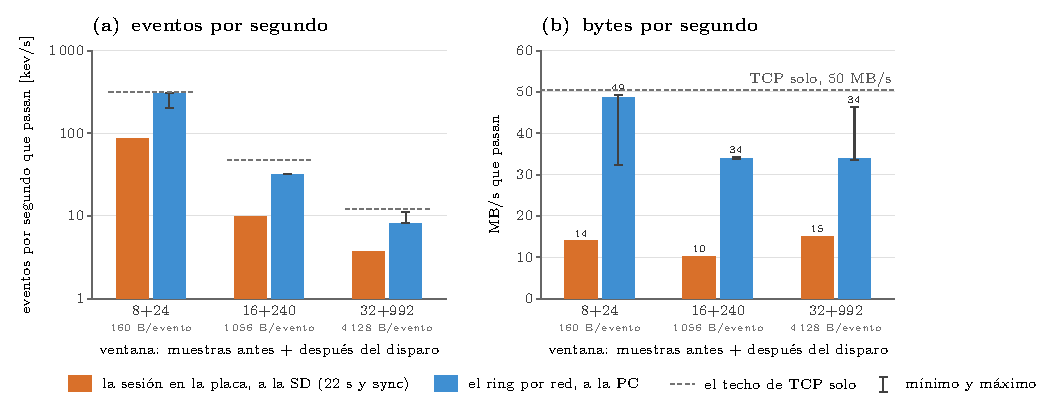
\includegraphics{cap10_bench_sd_red}
\caption[\emph{Benchmark} de escritura de archivos en la SD y por red]{%
\emph{Benchmark} de escritura de archivos. (a) En eventos por segundo, en escala
logarítmica; la raya es el techo de TCP sólo para ese tamaño de evento. (b) En
MB/s.\label{f:sw-bench-red}}
\end{figure}

% Bibliografía de este capítulo. Va al final del archivo, siempre.
\bibliografiacapitulo

%%% Local Variables:
%%% mode: latex
%%% TeX-master: "template"
%%% End:
      % Software
% Origen: Secciones/PI - Verificación de normativa nacional e internacional.md
\chapter{Verificación de normativa nacional e internacional}
\label{C:normativa}

% Figuras de ESTE capítulo + las compartidas. Siempre al principio del archivo.
\graphicspath{{figs/cap4/}{figs/comunes/}}

En este capítulo se analiza qué normativa nacional e internacional alcanza al
MCA, en qué carácter (obligación, guía de diseño o buena práctica) y qué parte
del trabajo responde a cada una.

\section{Análisis de ARN}
\label{S:norm-arn}

En Argentina, el único marco regulatorio nacional para la actividad nuclear es
el de la Autoridad Regulatoria Nuclear (ARN). La Ley N\textsuperscript{o} 24.804
le asigna la regulación de la seguridad radiológica y nuclear, y la faculta a
dictar normas de cumplimiento obligatorio~\cite{Ley24804}. Sus normas (serie AR)
son públicas. Para este trabajo son relevantes dos: la de diseño de reactores de
investigación, AR~4.2.2~\cite{ARN_AR422}, y la de sistemas de gestión,
AR~10.6.1~\cite{ARN_AR1061}. La ARN no tiene una norma específica para
instrumentación y control digital, software ni FPGA. Su enfoque está basado en
el desempeño: el responsable demuestra que cumple los objetivos de seguridad y
elige los estándares técnicos con que lo hace.

Las exigencias de la AR~4.2.2 recaen sobre los \textbf{sistemas importantes para
la seguridad}. Que un equipo lo sea depende de la \textbf{función que cumple en
la instalación}, no de cómo fue diseñado: es importante para la seguridad si su
función, o su falla, puede afectar la seguridad radiológica o nuclear. Un equipo
diseñado con el máximo rigor puede no serlo, y uno de laboratorio pasa a serlo
si se lo usa para una función de seguridad. El criterio~42 lo deja explícito:
``\emph{cuando un equipo o componente tiene varias funciones y una de las cuales
es de seguridad, debe ser clasificado como parte del sistema de
seguridad}''~\cite{ARN_AR422}.

El MCA clasifica pulsos por amplitud y entrega espectros y eventos a una PC,
Sec.~\ref{S:mca-descripcion-practica}. No actúa sobre ningún proceso, no tiene
alarmas y su salida no interviene en decisiones de operación. Por lo tanto
\textbf{no es un sistema importante para la seguridad}. Que no haya sido
diseñado para esa función es una consecuencia de esto, no la razón: tampoco está
calificado para cumplirla, como se discute en la Sec.~\ref{S:norm-iaea}.

La AR~4.2.2 ``\emph{es aplicable al diseño de reactores de investigación tipo
piscina y a las modificaciones de los sistemas importantes para la
seguridad}''~\cite{ARN_AR422}. Un instrumento de medición que no forma parte de
esos sistemas queda fuera de su alcance. Los criterios más cercanos a un MCA
marcan el límite, Tabla~\ref{t:norm-criterios-ar422}.

\begin{table}[H]
\centering
\caption[Criterios de la AR 4.2.2 más cercanos a un MCA]{%
Criterios de la AR~4.2.2 más cercanos a un MCA. A modo de comparación, el
criterio~34 exige a los sistemas de seguridad una tasa de falla por demanda
inferior a $10^{-3}$.\label{t:norm-criterios-ar422}}
\begin{tabularx}{\textwidth}{|>{\centering\arraybackslash}p{0.1\textwidth}|>{\raggedright\arraybackslash}X|>{\raggedright\arraybackslash}X|}
\hline \encabezado \textbf{Criterio} & \textbf{Qué establece} &
  \textbf{Por qué no alcanza al MCA} \\ \hline
42 & un equipo con una función de seguridad se clasifica como parte del
  sistema de seguridad & el MCA no tiene funciones de seguridad \\ \hline
50 & un sistema de calidad en el diseño que ``\emph{como mínimo, cubra los
  sistemas importantes para la seguridad}'' & el MCA no es uno de ellos \\ \hline
77 & un sistema de monitoreo de radiaciones con sensores en el reactor y
  alarmas locales & el MCA no tiene alarmas ni integra ese sistema \\ \hline
78 & tasa de falla de los sistemas de alarma y monitoreo de radiaciones
  inferior a $10^{-2}$ por demanda & se aplica al sistema del criterio~77 \\ \hline
79 a 81 & diseño de los dispositivos experimentales que se introducen en el
  reactor & tratan materiales, integridad estructural y confinamiento; el MCA
  es electrónica de lectura, afuera \\ \hline
\end{tabularx}
\end{table}

El MCA pasaría a ser importante para la seguridad si su salida alimentara una
alarma o el sistema de monitoreo de radiaciones, interviniera en decisiones de
operación, o formara parte de un sistema de protección. En ese caso aplicaría
como mínimo la meta de $10^{-2}$ por demanda del criterio~78, y el sistema de
gestión de la AR~10.6.1, obligatoria para todas las instalaciones y prácticas
reguladas~\cite{ARN_AR1061}.

Las fuentes radiactivas que se usan para probar el instrumento quedan bajo la
licencia de la institución que las tiene, según la Norma Básica de Seguridad
Radiológica AR~10.1.1~\cite{ARN_AR1011}. Esto no impone requisitos sobre el MCA.

\section{Análisis de IAEA}
\label{S:norm-iaea}

Como la ARN delega el detalle técnico, la referencia internacional es el
Organismo Internacional de Energía Atómica (IAEA). Su guía específica es la
SSG-37 (Rev.~1, 2023), sobre instrumentación, control y software importantes
para la seguridad en reactores de investigación~\cite{IAEA_SSG37}. Desarrolla
los requisitos de la SSR-3~\cite{IAEA_SSR3} y se aplica con \textbf{enfoque
graduado}: el rigor exigido es proporcional a la importancia para la
seguridad~\cite{IAEA_SSG22}. Para clasificar las funciones, la guía remite a
categorías como las de la IEC~61226~\cite{IEC61226}, que separa las funciones
en A, B y C según su importancia. Una función sin consecuencias para la
seguridad queda \textbf{no clasificada}, que es el caso del MCA. La conclusión
coincide con la de la Sec.~\ref{S:norm-arn}.

Para funciones de categoría B y C, el ciclo de vida de los circuitos programados
en HDL está definido en la IEC~62566-2~\cite{IEC62566-2}. El MCA no está
obligado a cumplirla, pero sirve como vara para ubicar lo que hicimos y lo que
no, Tabla~\ref{t:norm-ciclo-vida-62566}.

\begin{table}[H]
\centering
\caption[Ciclo de vida de la IEC 62566-2 frente a este trabajo]{%
Requisitos del ciclo de vida de la IEC~62566-2 frente a lo realizado en este
trabajo.\label{t:norm-ciclo-vida-62566}}
\begin{tabularx}{\textwidth}{|>{\raggedright\arraybackslash}p{0.25\textwidth}|>{\raggedright\arraybackslash}X|>{\raggedright\arraybackslash}p{0.22\textwidth}|}
\hline \encabezado \textbf{Requisito} & \textbf{En este trabajo} &
  \textbf{Estado} \\ \hline
especificación de requisitos & mapas de registros e interfaces de cada módulo,
  Sec.~\ref{S:ap-mca-mapa} &
  cubierto, sin trazabilidad formal requisito $\rightarrow$ prueba \\ \hline
verificación por simulación & testbenches por módulo,
  Sec.~\ref{S:intro-hw-verificacion} & cubierto \\ \hline
modelo de referencia independiente del RTL & modelo en Python comparado contra
  el RTL & cubierto \\ \hline
verificación en el dispositivo & generación interna y externa controlada,
  Sec.~\ref{S:res-etapas-validacion} & cubierto \\ \hline
validación con física real & medición con setup experimental & pendiente
  \\ \hline
verificación formal y análisis estático & --- & no realizado \\ \hline
equivalencia RTL $\leftrightarrow$ netlist & --- & no realizado \\ \hline
evaluación de componentes pre-desarrollados & placa, Linux y sistema de Red
  Pitaya usados tal como vienen, Sec.~\ref{S:hw-red-pitaya} & no evaluable
  \\ \hline
\end{tabularx}
\end{table}

La última fila deja una conclusión: la plataforma es adecuada para un
instrumento de medición, pero \textbf{no se podría calificar} para una función
de seguridad. Evaluar Linux y el sistema de Red Pitaya como software
pre-desarrollado, con el rigor de la IEC~62138~\cite{IEC62138}, no es viable.

% En la nota este bloque figura como "(sin título)", con la pregunta: "¿va en
% esta sección, con un título nuevo, o en otro capítulo?". Quedó como sección
% propia de este capítulo, con el título provisorio de la nota.
\section{Normas de medición y de equipo}
\label{S:norm-medicion}

Estas normas no son obligatorias para un prototipo de investigación, pero
definen qué tiene que medir bien un espectrómetro y cómo se informa,
Tabla~\ref{t:norm-medicion}.

\begin{table}[H]
\centering
\caption[Normas de medición y de equipo que guían el diseño del MCA]{%
Normas de medición y de equipo que guían el diseño del
MCA.\label{t:norm-medicion}}
\begin{tabularx}{\textwidth}{|>{\raggedright\arraybackslash}p{0.17\textwidth}|>{\raggedright\arraybackslash}X|>{\raggedright\arraybackslash}p{0.3\textwidth}|}
\hline \encabezado \textbf{Norma} & \textbf{Qué trata} &
  \textbf{Dónde se trata en este trabajo} \\ \hline
IEC 61452:2021~\cite{IEC61452} & calibración y uso de espectrómetros de
  germanio ($\approx$ \qty{45}{\kilo\electronvolt} a
  \qty{3}{\mega\electronvolt}); la Ed.~2 incorpora electrónica digital, Monte
  Carlo y límites de detección. Reemplaza a la ANSI/IEEE N42.14-1999,
  retirada~\cite{IEEEN4214} & Sec.~\ref{S:mca-tiempo-muerto},
  Sec.~\ref{S:mca-pileup},
  Sec.~\ref{S:implmca-perdidos},
  Sec.~\ref{S:implmca-teselado}
  \\ \hline
IEC 62755 / ANSI N42.42~\cite{IEC62755} & formato XML del espectro y sus
  metadatos (detector, calibración, tiempo real y vivo) &
  Sec.~\ref{S:sw-guardado} \\ \hline
GUM~\cite{GUM2008} & expresión de la incertidumbre de medición &
  Cap.~\ref{C:resultados} \\ \hline
IEC 61010-1~\cite{IEC61010-1} e IEC 61326-1~\cite{IEC61326-1} & seguridad
  eléctrica y compatibilidad electromagnética de equipos de laboratorio & la
  placa es un producto comercial; el trabajo cambia el bitstream y el
  software, no el hardware \\ \hline
\end{tabularx}
\end{table}

El riesgo eléctrico real del montaje es la alta tensión del detector, que no
forma parte del MCA.

% Bibliografía de este capítulo. Va al final del archivo, siempre.
\bibliografiacapitulo

%%% Local Variables:
%%% mode: latex
%%% TeX-master: "template"
%%% End:
      % Verificación de normativa nacional e internacional
% Origen: Secciones/PI - Conclusiones y Futuros Pasos.md
\chapter{Conclusiones y futuros pasos}
\label{C:conclusiones}

% Figuras de ESTE capítulo + las compartidas. Siempre al principio del archivo.
\graphicspath{{figs/cap11/}{figs/comunes/}}

%==============================================================================
\section{Conclusiones}
\label{S:concl}

Implementamos un analizador multicanal y un osciloscopio por eventos sobre la
Red Pitaya STEMlab 125-14. Todo el procesamiento de los pulsos corre en la PL:
el disparo, la medición de la amplitud y de la forma, el histograma y la captura
de las trazas. El PS se queda con el control, la adquisición y el guardado. El
sistema final es el TOP de integración con el anillo de eventos
(Cap.~\ref{C:top}), y lo caracterizamos
con \codigo{gen\_pulsos} en el lazo digital y en el canal analógico
OUT1 $\rightarrow$ IN1 (Cap.~\ref{C:resultados}).

\subsection{Parámetros del sistema implementado}
\label{S:concl-parametros}

En la Tabla~\ref{t:concl-parametros} se presentan los parámetros fijados en la
síntesis, que sólo cambian volviendo a sintetizar, y la ocupación de la FPGA.

\begin{table}[H]
\centering
\caption[Parámetros del sistema implementado]{%
Parámetros del sistema implementado: los que fija la síntesis del TOP de
integración con el anillo de eventos y su ocupación de la
Zynq-7010.\label{t:concl-parametros}}
\small
\begin{tabularx}{\textwidth}{|>{\raggedright\arraybackslash}p{0.16\textwidth}%
  |>{\raggedright\arraybackslash}p{0.22\textwidth}%
  |>{\raggedright\arraybackslash}X|}
\hline \encabezado \textbf{Bloque} & \textbf{Parámetro} & \textbf{Valor} \\ \hline
Plataforma & placa & Red Pitaya STEMlab 125-14: Zynq-7010, con dos núcleos ARM
  Cortex-A9 \\ \hline
 & ADC y DAC & 14 bits, 125~MS/s (\qty{8}{\nano\second} por muestra); entrada
  en LV, $\pm\qty{1}{\volt}$ (1~ADU $\approx$ \qty{122}{\micro\volt}) \\ \hline
MCA & espectro 1D & 8192 canales, con contadores de 32 bits que saturan
  \\ \hline
 & mapa 2D & $128 \times 64$ canales (amplitud $\times$ forma) \\ \hline
 & ranuras de medición & 3 \\ \hline
 & banco de trapecios & 3 formas, $(k, m) = (64, 48)$, $(32, 24)$ y $(8, 8)$,
  con un polo-cero común \\ \hline
 & publicador & uno, de 18 ciclos por evento \\ \hline
 & contabilidad del tiempo & \codigo{realtime} = \codigo{vetotime} +
  \codigo{t\_win} + \codigo{t\_div} + \codigo{t\_rearm} + \codigo{livetime}, al
  ciclo \\ \hline
Multitrigger & fuentes de disparo & nivel, pendiente ($L = 8$, $G = 4$),
  polo-cero ($k = 2$, $m = 1$), externa, generador y software, combinadas con
  una máscara OR \\ \hline
Osciloscopio & captura & por la BRAM, un evento por vez, y por el anillo de
  eventos en la DDR \\ \hline
 & ventanas del anillo & de $8 + 24$ a $32 + 992$ muestras (antes + después
  del disparo) \\ \hline
Generador & \codigo{gen\_pulsos} & tabla de 1024 alturas; caída, subida y ruido
  blanco programables; arribos periódicos o de Poisson; lazo digital \\ \hline
FPGA & LUT & 14\,358 de 17\,600 (\qty{81.6}{\percent}) \\ \hline
 & registros & 15\,513 de 35\,200 (\qty{44.1}{\percent}) \\ \hline
 & slices & 4400 de 4400 (\qty{100}{\percent}) \\ \hline
 & BRAM (bloques de 36~kb) & 33 de 60 (\qty{55}{\percent}) \\ \hline
 & DSP & 10 de 80 (\qty{12.5}{\percent}) \\ \hline
 & timing & cierra a \qty{125}{\mega\hertz}, con WNS = \qty{+0.008}{\nano\second}
  y WHS = \qty{+0.040}{\nano\second} \\ \hline
\end{tabularx}
\end{table}

El diseño ocupa las 4400 slices de la Zynq-7010, con el \qty{81.6}{\percent} de
las LUT, y cierra el timing a \qty{125}{\mega\hertz} con
\qty{8}{\pico\second} de margen. Para hacer lugar al anillo y a
\codigo{gen\_pulsos} sacamos la captura del osciloscopio por AXI, que el anillo
reemplaza, y bajamos el MCA de 4 a 3 ranuras y de 4 a 3 formas, lo que costó
cerca del \qty{1}{\percent} de la tasa en la línea. La placa quedó llena: un
bloque nuevo pide sacar otro o pasar a una FPGA más grande.

\subsection{Desempeño del hardware}
\label{S:concl-hw}

En la Tabla~\ref{t:concl-hw} se resumen las figuras de mérito que medimos con
\codigo{gen\_pulsos}. Salvo que se diga otra cosa, son con 3 ranuras, el banco
de trapecios y la base fija.

\begin{table}[H]
\centering
\caption[Figuras de mérito del MCA medidas con \codigo{gen\_pulsos}]{%
Figuras de mérito del MCA medidas con \codigo{gen\_pulsos}, en el lazo digital
y en el canal analógico OUT1 $\rightarrow$ IN1 con \qty{50}{\ohm}. Las
amplitudes van en ADU y las posiciones del histograma en canales. ---: todavía
sin medir en ese modo.\label{t:concl-hw}}
\small
\begin{tabularx}{\textwidth}{|>{\raggedright\arraybackslash}p{0.27\textwidth}%
  |>{\raggedright\arraybackslash}X|>{\raggedright\arraybackslash}X|}
\hline \encabezado \textbf{Figura de mérito} & \textbf{Lazo digital} &
  \textbf{Canal analógico} \\ \hline
Tasa aceptada, con 3~M/s de entrada & 1.9~M/s & casi la misma \\ \hline
Tasa en la línea, con 3~M/s de entrada & 1.2~M/s con el ASG y el polo-cero;
  0.78~M/s con la pendiente & máximo de 0.43 a 0.53~M/s, con 1.5~M/s de entrada
  \\ \hline
Error de $\hat\lambda$, con 3~M/s de entrada & ASG $-\qty{1.7}{\percent}$;
  polo-cero $-\qty{3.7}{\percent}$; pendiente $-\qty{18}{\percent}$ &
  polo-cero $+\qty{5.1}{\percent}$, por los disparos de más sobre el sobrepico
  \\ \hline
Separación de los disparos de un par & polo-cero \qty{40}{\nano\second};
  pendiente \qty{160}{\nano\second} & pendiente igual; el polo-cero vuelve a
  disparar \\ \hline
Separación de un par con las dos amplitudes en su línea &
  \qty{128}{\nano\second} (polo-cero) y \qty{160}{\nano\second} (pendiente);
  \qty{1.5}{\micro\second} con 1 ranura & pendiente igual; el polo-cero no lo
  resuelve \\ \hline
Umbral (mitad de los pulsos disparan) & polo-cero 48~ADU; pendiente 81~ADU &
  51 y 82~ADU \\ \hline
Walk del disparo & polo-cero \qty{8}{\nano\second}; pendiente
  \qty{48}{\nano\second} & 16 y \qty{55}{\nano\second} \\ \hline
INL del trapecio & $<\qty{0.002}{\percent}$~FS & $\pm\qty{0.008}{\percent}$~FS
  hasta 3200~ADU; $+\qty{0.66}{\percent}$ en 8000, donde satura el ADC
  \\ \hline
DNL del MCA & $<\qty{1.5}{\percent}$ rms (cota: domina la tabla del generador)
  & --- \\ \hline
Ganancia de ruido, $k = 8$, 32 y 64 & 0.48, 0.24 y 0.18 & igual \\ \hline
Piso de ruido $\sigma_0$, $k = 64$ & 0.06~ADU & 1.41~ADU \\ \hline
Resolución en una línea de 1500~ADU, $k = 64$ y ruido 2.3~ADU & FWHM
  \qty{0.07}{\percent} & FWHM \qty{0.24}{\percent} \\ \hline
Corrimiento de la línea con la tasa & $< 1.5$ canales hasta 3~M/s &
  $\sim 9$ canales a 400~k/s \\ \hline
Ajuste del polo-cero & error nulo en $\Delta M = +0.03$ a
  $+\qty{0.06}{\percent}$ & --- \\ \hline
\end{tabularx}
\end{table}

De estas mediciones sacamos cinco conclusiones.

\textbf{La cadena digital no agrega un error medible.} En el lazo digital la INL
del trapecio queda por debajo de \qty{0.002}{\percent}~FS y las líneas se
corren menos de 1.5 canales hasta 3~M/s. Lo que se aparta del ideal en el canal
analógico es del canal, no del diseño. Esto también resuelve una limitación de
la generación externa controlada, que no separaba la INL del generador de la del
ADC: el canal de la placa da $\pm\qty{0.008}{\percent}$~FS hasta 3200~ADU, así
que lo que mida de más un generador externo en ese rango es del generador.

\textbf{Lo que limita la tasa es el apilamiento, no el tiempo muerto.} A 3~M/s
de entrada, pasar de 1 a 3 ranuras sube los eventos aceptados de 0.73 a
1.9~M/s: las ranuras sacan del camino casi todo el tiempo muerto. Lo que queda
es la diferencia entre los aceptados y los que caen en su línea, 1.9 contra
1.2~M/s, y es casi toda apilamiento: pulsos que el MCA mide con otro encima. Esa
pérdida es estadística, depende de la tasa y del largo de la forma, y no baja
con más ranuras.

\textbf{El disparo fija el comportamiento a alta tasa.} El polo-cero separa dos
disparos a \qty{40}{\nano\second} y registra en su línea lo mismo que el ASG,
que dispara con cada pulso sin mirar la señal (1.23 contra 1.21~M/s a 3~M/s). La
pendiente necesita \qty{160}{\nano\second} y es paralizable: su tasa en la línea
llega a 0.97~M/s con 2~M/s de entrada y baja a 0.78 con 3~M/s. Eso llega a la
tasa estimada: $\hat\lambda$ corrige el tiempo muerto de las ranuras y del
publicador, y queda a $-\qty{1.7}{\percent}$ de la tasa real con el ASG y a
$-\qty{3.7}{\percent}$ con el polo-cero, pero con la pendiente queda
\qty{18}{\percent} abajo, porque el re-armado del disparo sólo se cuenta cuando
hay una ranura libre. Con un canal sin sobrepico, el polo-cero es la fuente de
disparo para medir.

\textbf{En el canal analógico, lo que limita es el canal.} El canal
OUT1 $\rightarrow$ IN1 con \qty{50}{\ohm} tiene una ganancia de 0.95, cae
\qty{3}{\decibel} en \qty{52}{\mega\hertz} y tiene un piso de 4.7~ADU rms. Dos
rasgos suyos explican casi todo lo que el modo analógico agrega:
\begin{itemize}
  \item \textbf{El sobrepico del \qty{24}{\percent}.} El polo-cero vuelve a
    disparar sobre él desde unas 3200~ADU y deja de resolver pares, y desde unas
    6990~ADU el ADC satura. La pendiente no lo ve.
  \item \textbf{La caída lenta del \qty{7.3}{\percent}, en 3 a
    \qty{13}{\micro\second}.} Las colas negativas de los pulsos se apilan y
    bajan la base con la tasa, y el trapecio pasa ese error a la amplitud. Con
    base fija la línea se corre unos 9 canales a 400~k/s, y la tasa en la línea
    no pasa de 0.43 a 0.53~M/s.
\end{itemize}

Estos dos rasgos son del montaje de generación interna, y todavía no separamos
cuánto viene de la salida y cuánto de la entrada; con un detector sólo se usa la
entrada. La conclusión, igual, vale para cualquier canal: antes de medir hay que
caracterizarlo, y una cola lenta hay que compensarla antes del MCA, como el
polo-cero compensa la caída del pulso.

\subsection{Desempeño del software}
\label{S:concl-sw}

En el software medimos cuánto cuesta cada capa del camino de los datos. Los
resultados se resumen en la Tabla~\ref{t:concl-sw}.

\begin{table}[H]
\centering
\caption[Desempeño del software en la placa]{%
Desempeño del software en la placa, por capa del camino de los datos. «Al día»
es la tasa más alta del barrido sin descartes ni atraso; «saturado», lo que lee
la capa cuando no da abasto.\label{t:concl-sw}}
\small
\begin{tabularx}{\textwidth}{|>{\raggedright\arraybackslash}p{0.33\textwidth}%
  |>{\raggedright\arraybackslash}X|}
\hline \encabezado \textbf{Camino} & \textbf{Medido} \\ \hline
leer un registro & \qty{1.5}{\micro\second} en C, \qty{56.8}{\micro\second} por
  el binding y \qty{10.5}{\micro\second} en Python puro \\ \hline
leer el espectro (8192 canales) & \qty{1.70}{\milli\second} en C,
  \qty{1.88}{\milli\second} por el binding y \qty{34.3}{\milli\second} en Python
  puro; \qty{3.5}{\milli\second} por la red \\ \hline
osciloscopio por la BRAM, con el lazo en C & \qty{18.2}{\micro\second} de tiempo
  muerto por evento (mediana); 34~k/s guardados \\ \hline
anillo, la PL sola & 1.42~M/s con ventanas de $8 + 24$ muestras; 49~k/s con
  $32 + 992$ \\ \hline
anillo, el lector de C copiando & 753~k/s con $8 + 24$ \\ \hline
anillo, el lector de C copiando y verificando & 300~k/s al día con $8 + 24$
  (439~k/s saturado); de 70 a 98~MB/s saturado \\ \hline
anillo, la sesión de Python guardando en \ruta{.npz} & 100~k/s al día con
  $8 + 24$ (167~k/s saturado en la SD y 203~k/s en \ruta{/dev/shm}); 10~k/s con
  $32 + 992$ \\ \hline
$10^8$ eventos con los dos núcleos ocupados & la PL sola a 1.4~M/s y el lector
  de C a 200~k/s, sin descartes ni errores \\ \hline
\end{tabularx}
\end{table}

\textbf{Lo que limita al osciloscopio es el PS.} Cada capa que se suma al camino
de los datos baja la tasa: la PL sola escribe 1.42~M/s en el anillo, el lector
de C copia 753~k/s y, verificando cada slot, 300~k/s, y la sesión de Python
guarda 100~k/s. El escritor de la PL llega en la placa al techo de la simulación
con todas las ventanas, así que el AXI y la DDR no lo frenan; con la sesión,
\ruta{/dev/shm} da casi lo mismo que la SD, así que tampoco frena el disco. Lo
que limita es el software en los dos núcleos del ARM. El MCA no tiene este
problema, porque acumula el histograma en la PL y el PS sólo lee el espectro:
acepta 1.9~M/s, contra los 100~k/s de trazas que guarda el osciloscopio.

\textbf{El costo del binding es por llamada, no por dato.} Pasar por
\codigo{ctypes} agrega unos \qty{55}{\micro\second} por llamada, que dominan al
leer un registro y casi no pesan al leer el espectro (un \qty{10}{\percent} sobre
C). Por eso los lazos por evento están en C, y en Python quedan la sesión, los
archivos y la aplicación. Con el lazo de la BRAM en C, el tiempo muerto por
evento bajó de 252.7 a \qty{18.2}{\micro\second}.

\textbf{El anillo absorbe las demoras del PS, hasta un punto.} Con $10^8$
eventos y los dos núcleos ocupados por otros procesos, la PL a 1.4~M/s no
descarta ninguno: el anillo absorbió una demora de \qty{30}{\milli\second} del
lector. El lector de C cumple a 200~k/s, pero sin margen: una demora de medio
segundo llenó el anillo al \qty{81}{\percent}. Con el ARM ocupado, la tasa
segura para leer trazas de 32 muestras desde C está por debajo de 200~k/s.

En resumen, el procesamiento en la PL rinde lo que permite la estadística de los
arribos. Lo que queda por mejorar está en el canal analógico, en la estabilidad
con la temperatura, que todavía no medimos, y en el camino de las trazas por el
PS.

%==============================================================================
\section{Posibles futuros pasos}
\label{S:concl-futuros}

A continuación se describen algunos de los pasos que quedan para llevar el
sistema a una medición real y para mejorarlo.
\begin{itemize}
  \item \textbf{Implementar el sistema en un setup experimental real.} Es la
    última etapa de validación: un detector con su preamplificador en IN1 y
    fuentes de calibración. Con pulsos reales se miden la resolución en energía,
    la linealidad y la tasa, y se ve cuánto de lo que agrega el canal analógico
    aparece también con el detector, que sólo usa la entrada.
  \item \textbf{Comparar el funcionamiento con otros MCA comerciales.} Con el
    mismo detector y la misma fuente, contra un MCA digital comercial. Antes se
    puede comparar en papel con sus especificaciones, cuidando que las cifras
    sean comparables: la INL, por ejemplo, la dan sobre casi todo el rango, y la
    nuestra está medida hasta 3200~ADU.
  \item \textbf{Obtener feedback de usuarios y comprobar la facilidad de uso de
    la API y la GUI.} Darle el sistema a usuarios del laboratorio con una tarea
    fija, como calibrar el canal, adquirir un espectro y guardar las trazas, y
    medir cuánto tardan y dónde se traban, con la GUI y con la API.
  \item \textbf{Crear una aplicación web al estilo de las de Red Pitaya.} Como un
    cliente más del protocolo JSON del servidor, el mismo que usa la GUI, sin
    cambiar nada en la placa.
  \item \textbf{Crear una documentación oficial para el código de la API.} La
    documentación ya está en el repositorio; falta publicarla como un sitio
    generado a partir del código.
  \item \textbf{Compensar la caída lenta del canal.} La base dinámica, que
    corrige la base según la tasa estimada, ya está implementada en el software y
    falta validarla en la placa. Corrige la base en promedio, pero no su
    fluctuación de un pulso a otro. Para eso hay que invertir los polos lentos
    del canal antes del MCA, con un filtro como el polo-cero del trapecio.
  \item \textbf{Estabilizar el espectro.} Primero hay que medir la deriva del
    sistema con la temperatura. Con eso, un lazo en el PS puede mantener un pico
    de referencia en su canal, corrigiendo una ganancia fina y un desplazamiento
    antes del histograma, como hacen los MCA comerciales. Para estabilizar la
    electrónica alcanza con un pulser como \codigo{gen\_pulsos}; para
    estabilizar también el detector hace falta una línea de la fuente.
  \item \textbf{Contar el re-armado del disparo en $\hat\lambda$ aunque no haya
    ranura libre.} Hoy \codigo{t\_rearm} sólo cuenta cuando hay una ranura
    libre, y con la pendiente $\hat\lambda$ queda \qty{18}{\percent} abajo a
    3~M/s. Un contador del re-armado que corra también con las ranuras ocupadas
    debería corregir el tiempo muerto del disparo entero.
  \item \textbf{Testear en otras plataformas con mayor cantidad de recursos.} La
    Zynq-7010 quedó llena. Probar el diseño en una plataforma con más recursos,
    como una con la Zynq-7020, que tiene unas tres veces más lógica, permitiría
    recuperar la ranura y la forma del banco que sacamos, y agregar los bloques
    de esta lista.
  \item \textbf{Medir la salida de las trazas por la red.} El camino del anillo
    de eventos por la red está implementado y probado sin la placa. Falta medir
    en la placa cuánto da, contra los 100~k/s de la sesión que guarda en la SD.
  \item \textbf{Agregar coincidencias y anticoincidencias.} Con dos detectores
    en IN1 e IN2, o con un detector y un blindaje activo. El análisis y el
    diseño están hechos; se llevan al RTL cuando haya un montaje que los use.
\end{itemize}

%%% Local Variables:
%%% mode: latex
%%% TeX-master: "template"
%%% End:
      % Conclusiones y futuros pasos


\appendix
% Origen: sección "Apéndice" (Capturas Aplicación) de
% Secciones/PI - Tipos de Usuario y APP.md
% El archivo se llama apend4 por orden de creación; en template.tex va como
% primer apéndice, igual que su capítulo va primero.
\chapter{Capturas de la aplicación}
\label{C:ap-app}

% Figuras de este apéndice + las compartidas.
\graphicspath{{figs/apendices/}{figs/comunes/}}

% Las capturas van con [H], fijas debajo del párrafo que las describe: el texto
% es corto y como floats se acumulaban y quedaban solas al final del apéndice.

Las capturas se tomaron con la APP conectada al MCA simulado
(\cmd|make app-demo|); por eso la barra superior indica \codigo{127.0.0.1} y
``\emph{simulated}'', y los valores que se ven ilustran la interfaz, no son mediciones.
Esa barra es común a todas las pestañas: el botón de conexión, la IP y el puerto
del servidor, y un resumen del \emph{bitstream} cargado (la versión del MCA, la cantidad
de canales del histograma, las ranuras y la fuente del disparo del MCA).

A continuación presentamos las capturas de las pestañas de adquisición: el
espectro del MCA, el mapa 2D y los pulsos del OSC.

En la Fig.~\ref{f:ap-app-spectrum} se presenta la pestaña \emph{Spectrum}. A la
izquierda está el histograma 1D, con las herramientas de matplotlib para
navegarlo, la escala logarítmica, el agrupamiento de canales y el período de
refresco. A la derecha están la lectura bajo el cursor, el total de cuentas y la
tasa de entrada instantánea y media; los contadores (aceptados, rechazados por
amplitud y por forma, apilados, perdidos) y los tiempos real, vivo y muerto; la
duración de la adquisición, con los botones \emph{Start}, \emph{Stop}, \emph{Clear}, \emph{Save}, \emph{Load} e
\emph{Image}; y la lista de picos detectados con su canal, FWHM, resolución, cuentas en
la cima y área. Cada pico de la lista se marca sobre el espectro, con su FWHM
dibujado como una barra a media altura.

\begin{figure}[H]
\centering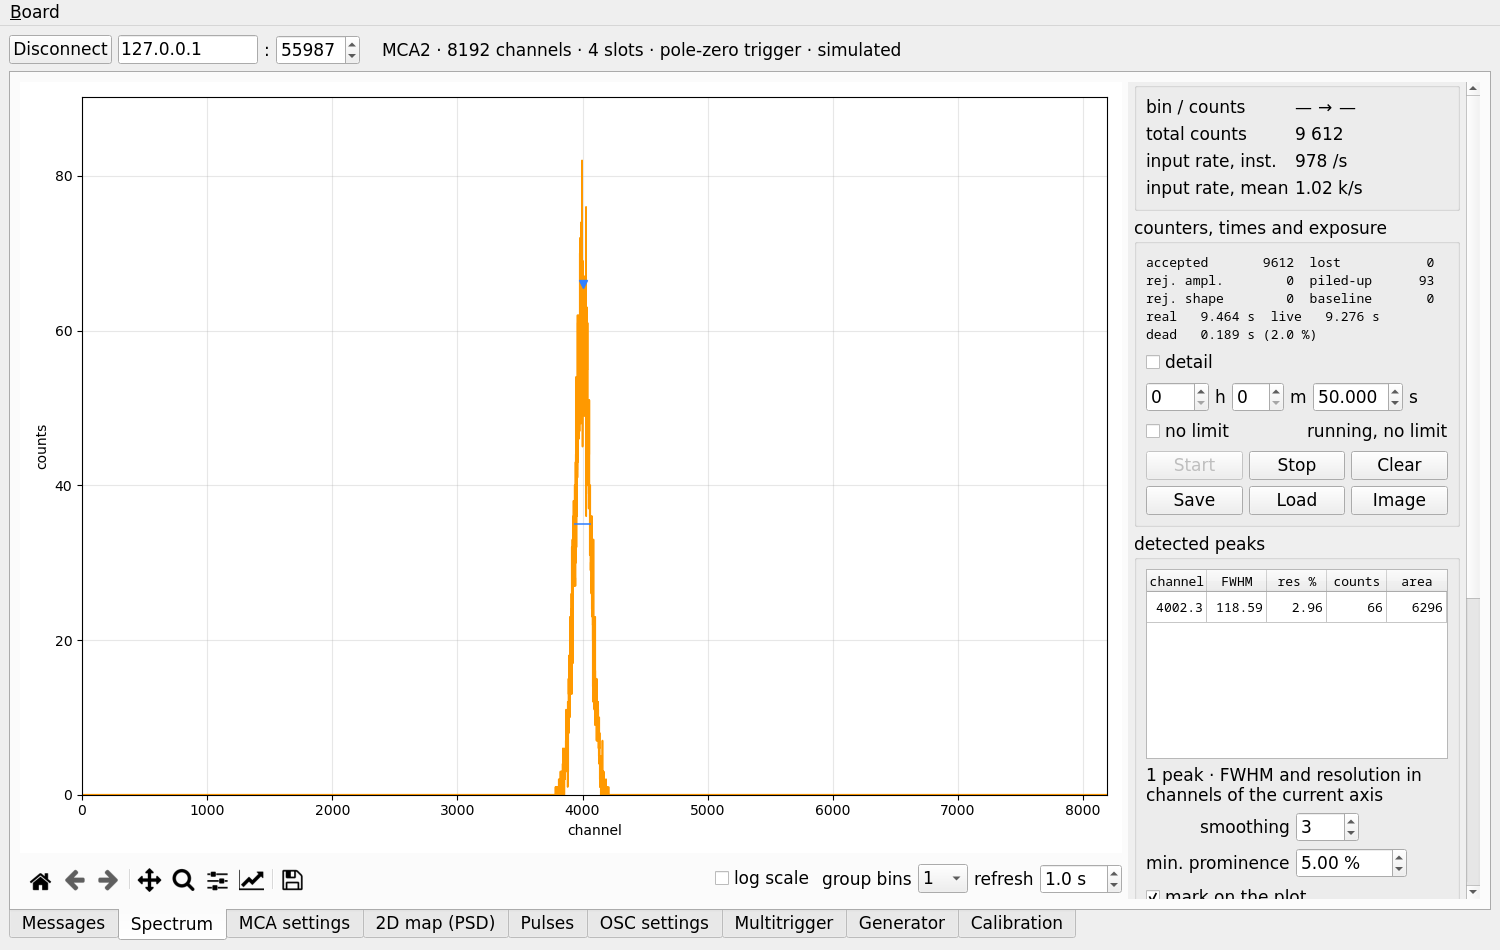
\includegraphics{apD_mcamon_spectrum}
\caption[Pestaña \emph{Spectrum}]{%
Pestaña \emph{Spectrum}: el histograma 1D con los contadores, los tiempos, los
controles de la adquisición y la lista de picos
detectados.\label{f:ap-app-spectrum}}
\end{figure}

En la Fig.~\ref{f:ap-app-2d-map} se presenta la pestaña 2D \emph{map} (PSD): el mapa de
amplitud $\times$ factor de forma ($Q_\text{tail}/Q_\text{total}$), con las
cuentas en escala logarítmica. En la captura, el MCA simulado genera dos
poblaciones de pulsos con la misma amplitud y distinta forma, que en el mapa
aparecen como dos manchas separadas a lo largo del eje del factor de forma. A la
derecha se calcula la figura de mérito (FOM) de esa separación, sobre la franja
de amplitudes que se elija.

\begin{figure}[H]
\centering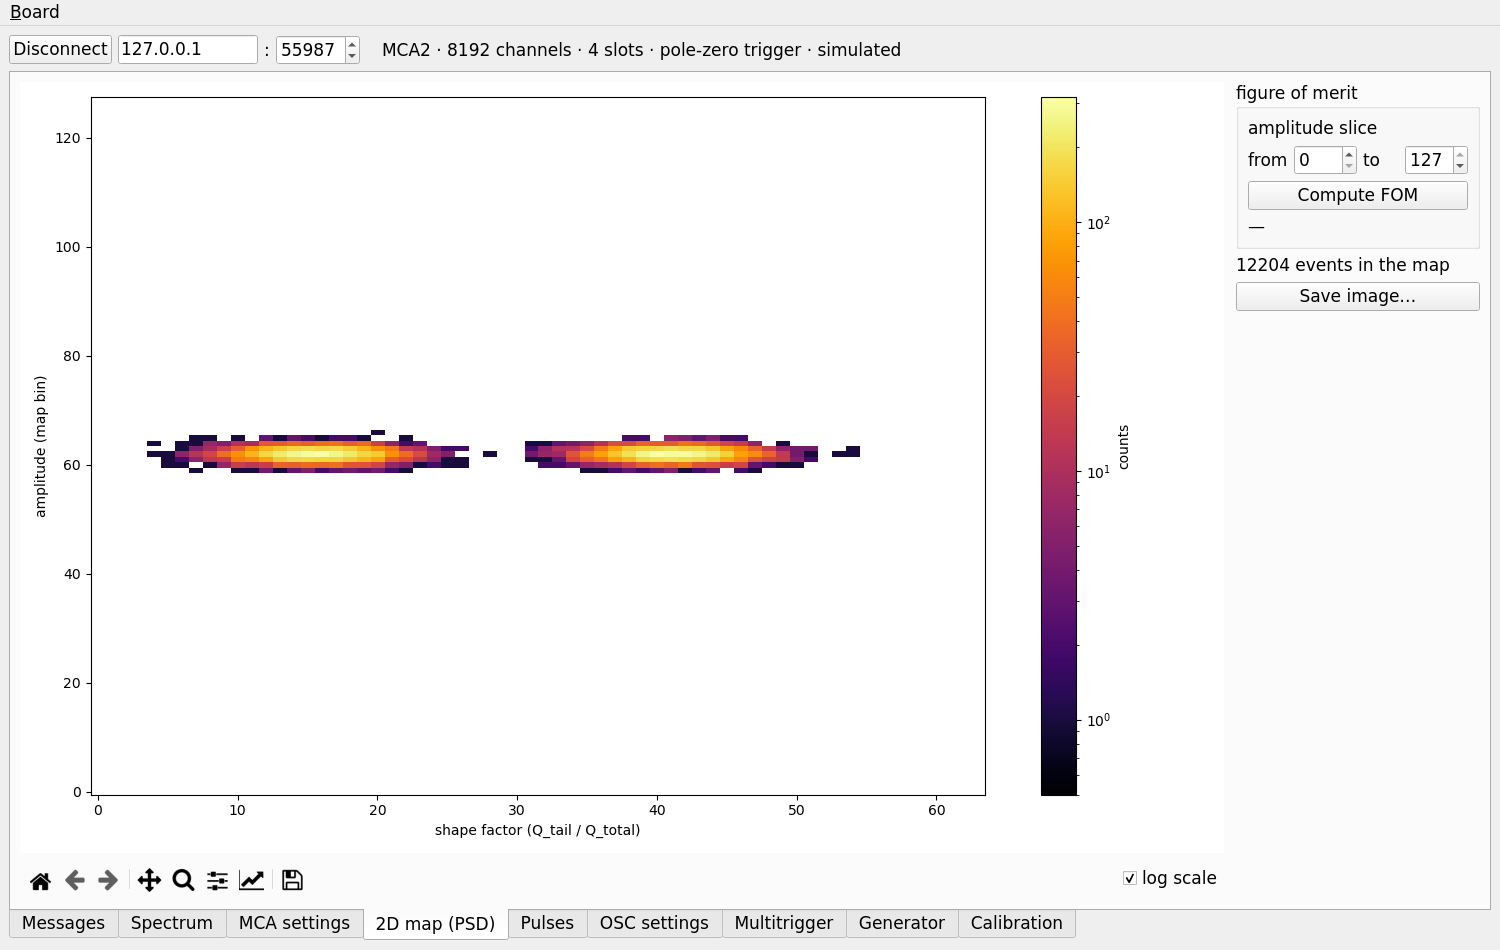
\includegraphics{apD_mcamon_2d_map_psd}
\caption[Pestaña 2D \emph{map} (PSD)]{%
Pestaña 2D \emph{map} (PSD): el mapa de amplitud $\times$ factor de forma con dos
poblaciones de pulsos simuladas, y el cálculo de la figura de mérito sobre una
franja de amplitudes.\label{f:ap-app-2d-map}}
\end{figure}

En la Fig.~\ref{f:ap-app-pulses} se presenta la pestaña \emph{Pulses}. Arriba está la
última captura del osciloscopio en IN1 e IN2, en volts contra el tiempo desde el
disparo, con la persistencia de las capturas anteriores; a la derecha se eligen
las muestras antes y después del disparo, la captura continua y la vista (pulso
o mapa de calor). Abajo está la tasa en el tiempo: los eventos aceptados por el
MCA, su media y los disparos del OSC. La línea vertical punteada marca en qué
momento de esa curva se tomó la captura de arriba.

\begin{figure}[H]
\centering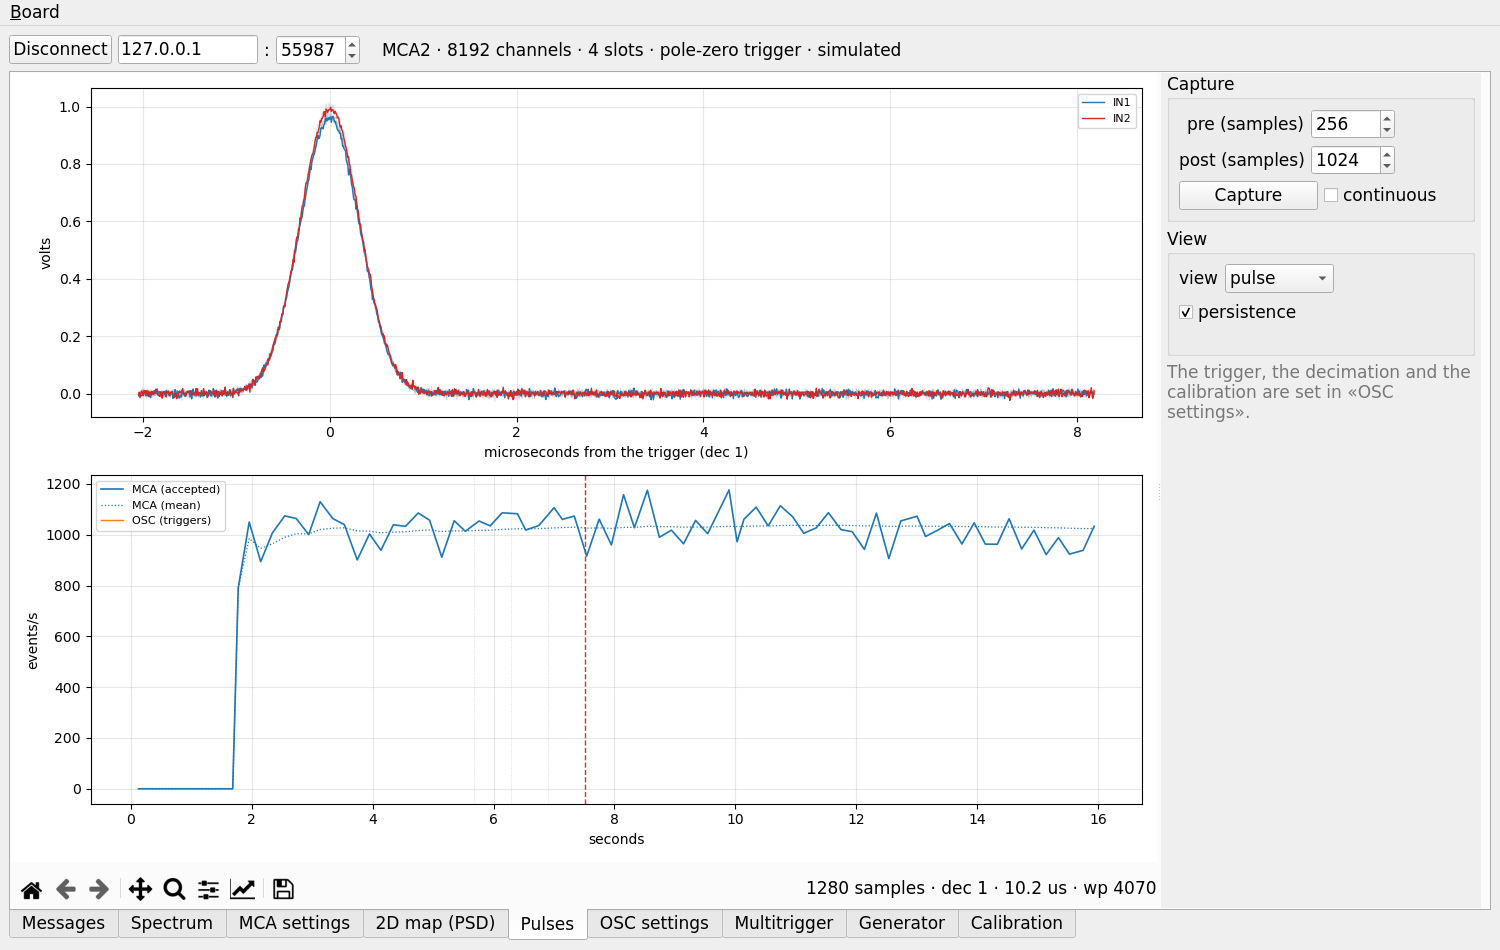
\includegraphics{apD_mcamon_pulses}
\caption[Pestaña \emph{Pulses}]{%
Pestaña \emph{Pulses}: arriba, la última captura del osciloscopio en IN1 e IN2; abajo,
la tasa de eventos en el tiempo, con el momento de la captura
marcado.\label{f:ap-app-pulses}}
\end{figure}

A continuación presentamos las pestañas de configuración del MCA,
del OSC, del multitrigger, del generador de pulsos y de calibración, y la de
mensajes. Las pestañas de configuración comparten la misma organización: arriba,
una franja con el camino de los datos por etapas, con los colores del diagrama de
panorama del módulo y la tasa de cada tramo sobre su flecha; debajo de cada
etapa, en rojo, lo que se pierde o lo que deja al sistema sin eventos. Abajo, los
parámetros agrupados por etapa, cada grupo con el color de su bloque en la
franja.

En la Fig.~\ref{f:ap-app-mca-settings} se presenta la pestaña MCA \emph{settings}. La
franja recorre el MCA: la entrada (canal, decimación y retardo), la base
(seguidor automático o fija), el banco de trapezoides ---en gris, porque el
\emph{bitstream} de la captura no lo trae---, la segmentación, en la que cada disparo
del multitrigger abre una ranura, las compuertas de las ranuras y la publicación
(eje, discriminador e histograma). Bajo la segmentación se ven las pérdidas por
re-armado, por falta de ranura libre y del publicador, y bajo la publicación,
las de colisiones. Abajo, los parámetros en tres columnas: preprocesamiento
(entrada y base), segmentación y ranuras (cantidad de ranuras y compuertas \emph{short}
y \emph{long}), y publicación (eje del histograma, discriminador e histograma). La
leyenda marca qué cambios mezclan dos configuraciones en el histograma (●) y
cuáles, mal puestos, dejan el sistema sin eventos (⚠).

\begin{figure}[H]
\centering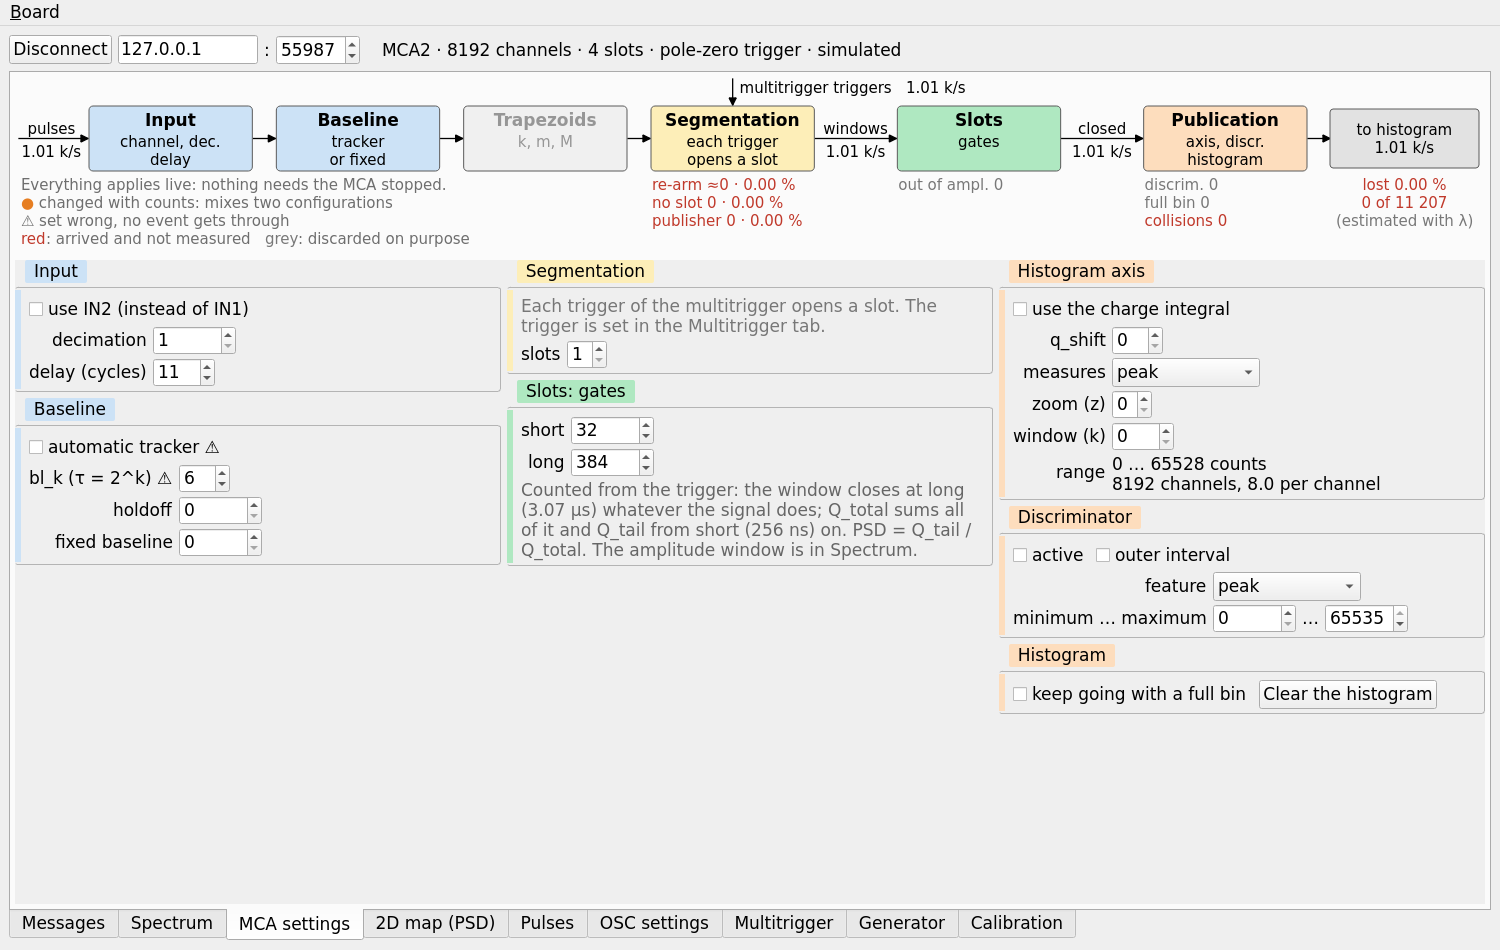
\includegraphics{apD_mcamon_mca_settings}
\caption[Pestaña MCA \emph{settings}]{%
Pestaña MCA \emph{settings}: la franja del MCA con la tasa y las pérdidas de cada
etapa, y debajo sus parámetros agrupados en preprocesamiento, segmentación y
ranuras, y publicación.\label{f:ap-app-mca-settings}}
\end{figure}

En la Fig.~\ref{f:ap-app-osc-settings} se presenta la pestaña OSC \emph{settings}. La
franja de arriba sigue al osciloscopio: la entrada (\emph{offset}, ganancia y filtro),
la decimación, el disparo que llega del multitrigger y la captura en BRAM, que
alimenta la pestaña \emph{Pulses}. La de abajo sigue al \emph{ring}, cuando el \emph{bitstream} lo
trae: el disparo o el generador de eventos abren una ventana con muestras antes y
después del disparo, que se escribe en el \emph{ring} de la DDR y se vuelca a archivos
en una carpeta de la placa. Abajo están los registros por etapa: el \emph{offset} y la
ganancia de calibración de cada canal, la decimación, el estado de la captura y
la configuración del \emph{ring} (estímulo, ventana, carpeta, formato de archivo y
memoria), con \emph{Start} y \emph{Stop} para su adquisición.

\begin{figure}[H]
\centering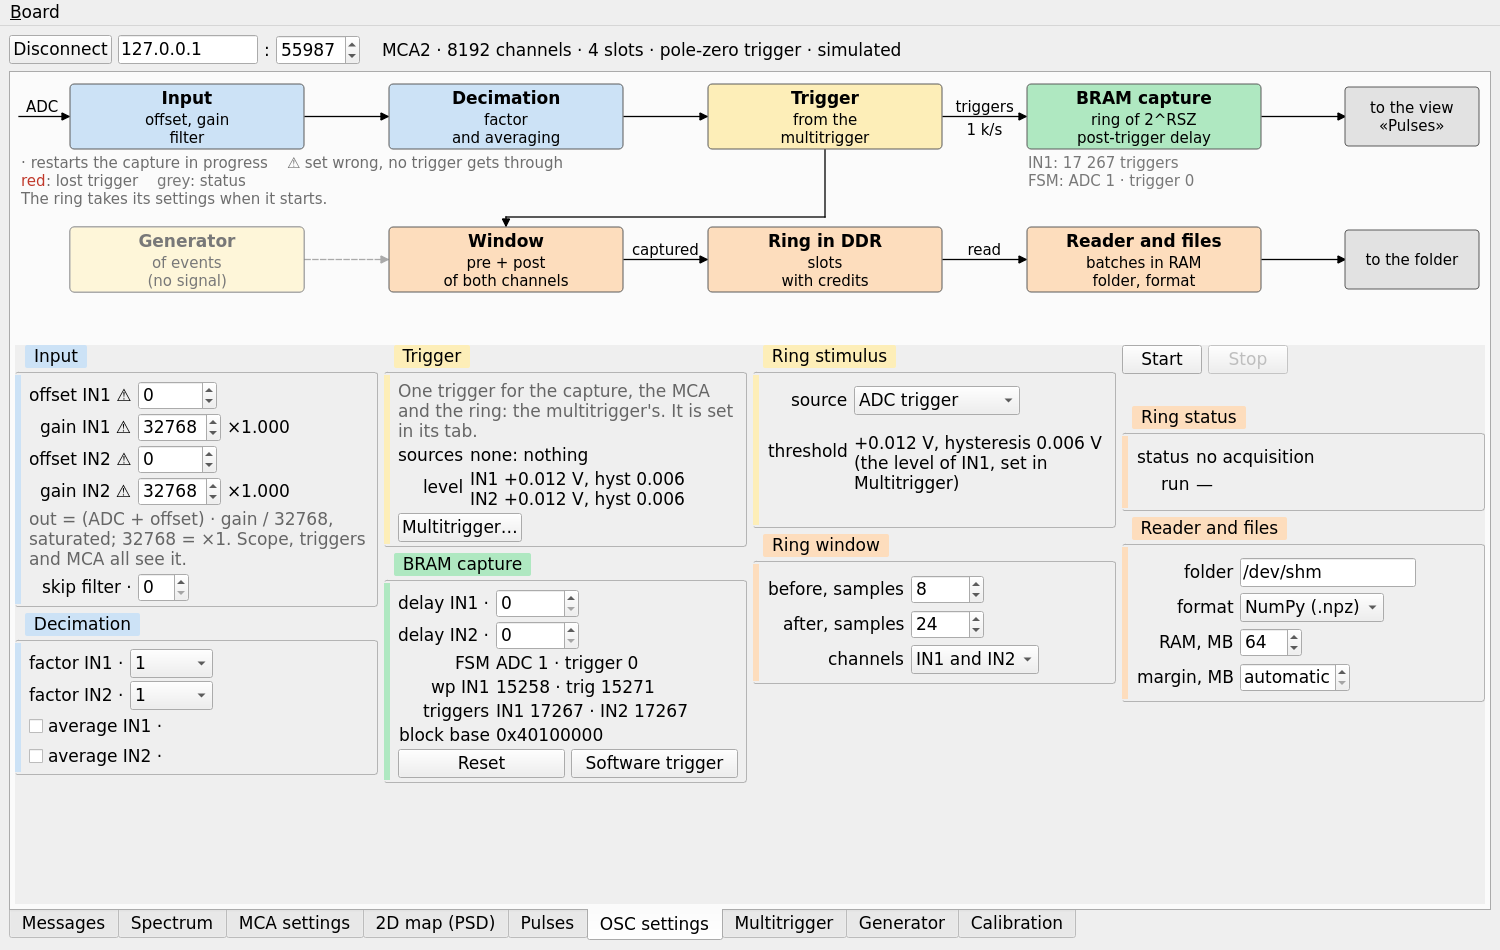
\includegraphics{apD_mcamon_osc_settings}
\caption[Pestaña OSC \emph{settings}]{%
Pestaña OSC \emph{settings}: arriba, las franjas del osciloscopio y del \emph{ring}; abajo,
los registros por etapa y la adquisición del \emph{ring} a una carpeta de la
placa.\label{f:ap-app-osc-settings}}
\end{figure}

En la Fig.~\ref{f:ap-app-multitrigger} se presenta la pestaña Multitrigger,
donde se configura el único disparo del sistema, que comparten la captura del
osciloscopio, el MCA y el \emph{ring}. La franja va desde las entradas (IN1, IN2, DIO0,
el generador y el disparo por software) a las fuentes (nivel, pendiente,
polo-cero), a la máscara OR que elige qué fuentes disparan cada canal y al
evento que llega a la captura y al MCA; debajo está el \emph{shield}, que re-arma los
canales después de un \emph{holdoff} y puede vetar al MCA. En la captura, la franja
señala en rojo que ninguna fuente está en las máscaras, así que no hay disparos.
Abajo, por etapa: los umbrales e histéresis del disparo por nivel, con su
equivalente en volts; el disparo del MCA (pendiente o polo-cero) con sus
parámetros; la grilla de la máscara, fuentes $\times$ canal y flanco; el evento;
y el \emph{shield}.

\begin{figure}[H]
\centering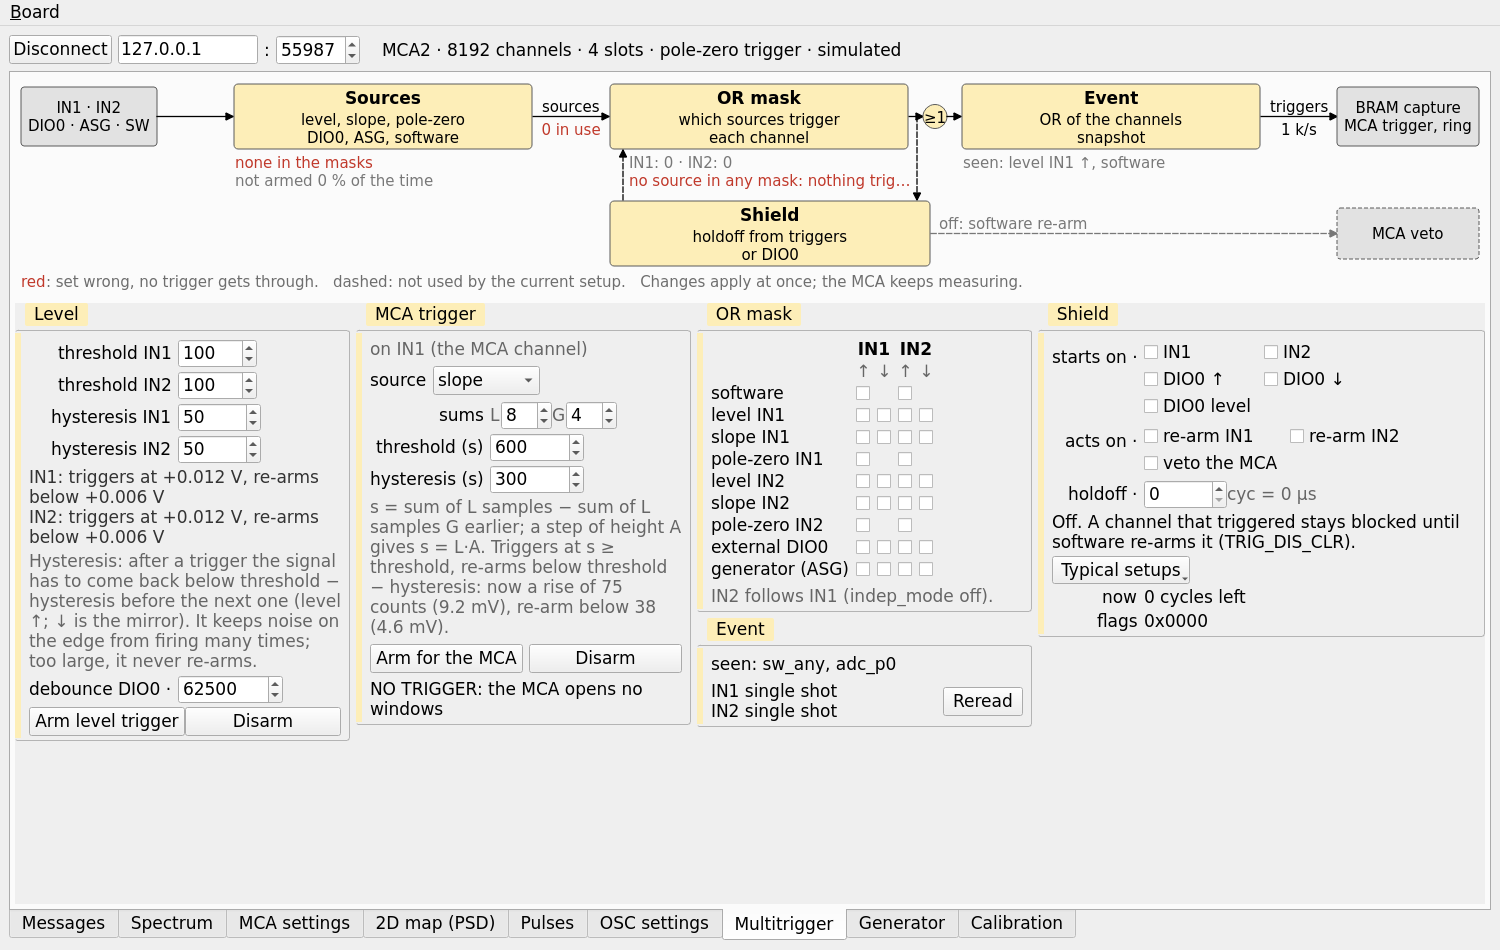
\includegraphics{apD_mcamon_multitrigger}
\caption[Pestaña Multitrigger]{%
Pestaña Multitrigger: la franja del disparo, de las entradas al evento, con el
\emph{shield}; abajo, las fuentes, la máscara OR por canal, el evento y el
\emph{shield}.\label{f:ap-app-multitrigger}}
\end{figure}

En la Fig.~\ref{f:ap-app-generator} se presenta la pestaña \emph{Generator}. La franja
sigue el orden de la ecuación del generador de pulsos,
\begin{equation}
  v(t) = B + \sum_k A_k\, h(t - t_k) + r(t),
  \label{e:ap-app-generador}
\end{equation}
con los disparos $t_k$ (periódicos o Poisson), las amplitudes $A_k$ sorteadas de
una tabla de 1024 alturas, la forma $h$ con su decaimiento $\tau_d$ y su subida
$\tau_r$, y la salida, con la base $B$, el ruido $r$ y la saturación a 14 bits,
hacia el DAC (OUT1, OUT2). Abajo están los controles de cada etapa, el lazo
digital, que lleva el generador a la entrada del MCA sin pasar por el DAC, y el
estado del generador. ``\emph{Apply}'' escribe la configuración entera y detiene el
generador.

\begin{figure}[H]
\centering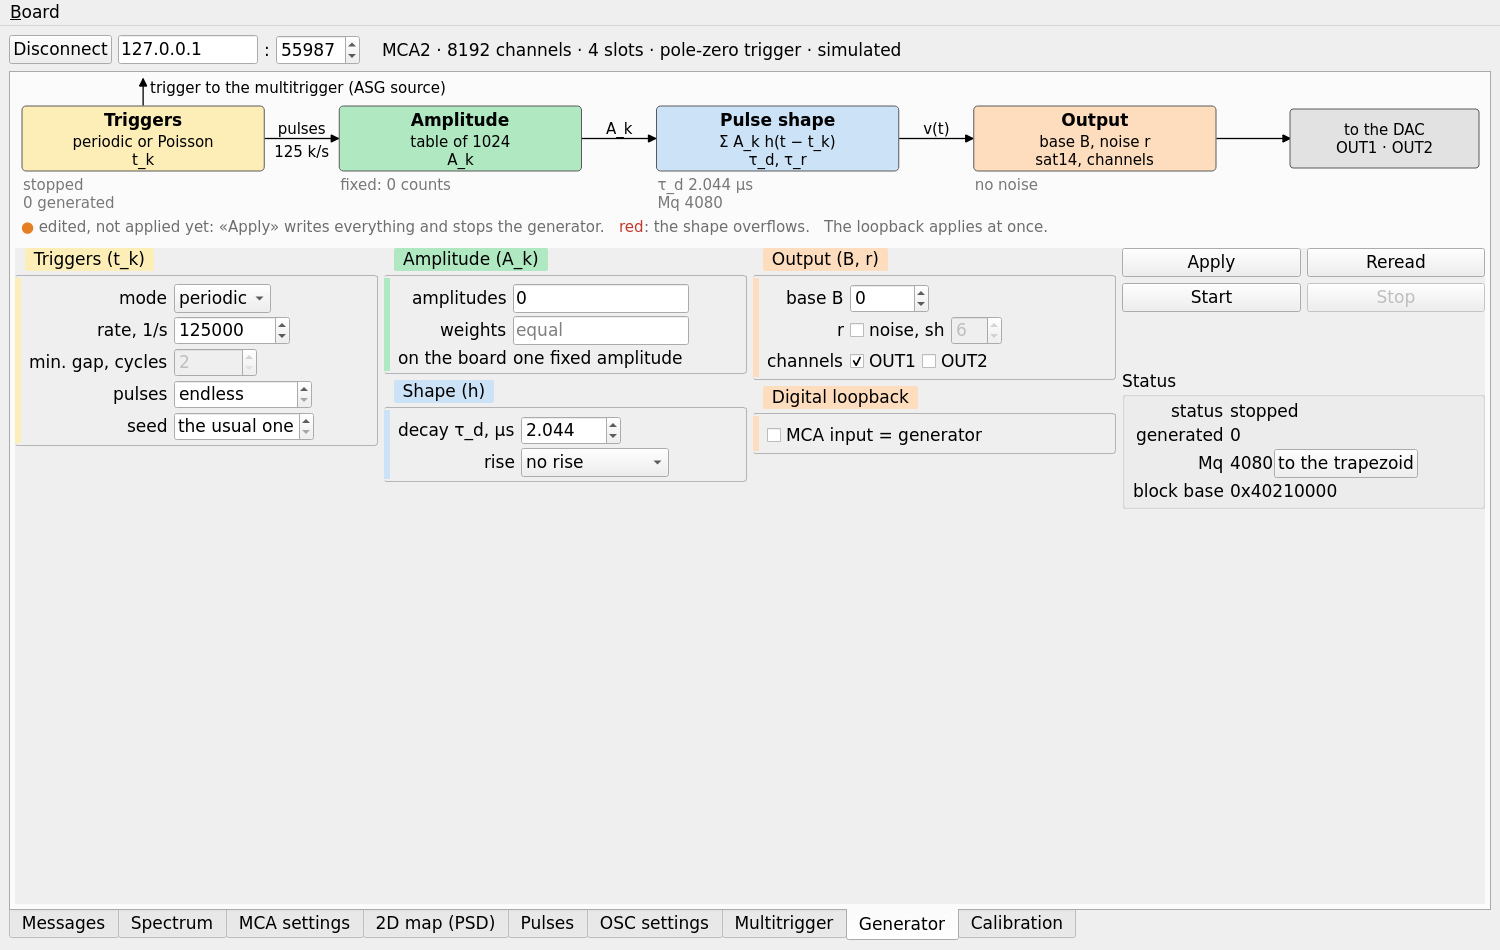
\includegraphics{apD_mcamon_generator}
\caption[Pestaña \emph{Generator}]{%
Pestaña \emph{Generator}: la franja del generador de pulsos en el orden de su
ecuación, los controles por etapa y el lazo digital hacia el
MCA.\label{f:ap-app-generator}}
\end{figure}

En la Fig.~\ref{f:ap-app-calibration} se presenta la pestaña \emph{Calibration}. La
franja va de la referencia (el generador por OUT1 o una cuadrada externa) al
canal analógico (cable, carga, \emph{front-end} y ADC), al modelo del canal (un FIR más
polos lentos, que producen una caída lenta) y a la base del MCA, fija o
dinámica. Abajo, a la izquierda, están la referencia, la conexión medida y la
tabla con el origen de la caída lenta, una fila por conexión; al centro, los
resultados (\emph{offset} y ruido, ganancia, caída lenta y por polo, latencia, subida,
ancho de banda, residuo y diafonía) y la configuración de la base del MCA; a la
derecha, la respuesta al escalón rápida y lenta, la respuesta en frecuencia del
FIR, el piso de ruido de IN1 y la variación de la base dinámica en el último
minuto. Los valores de la captura salen del canal simulado.

\begin{figure}[H]
\centering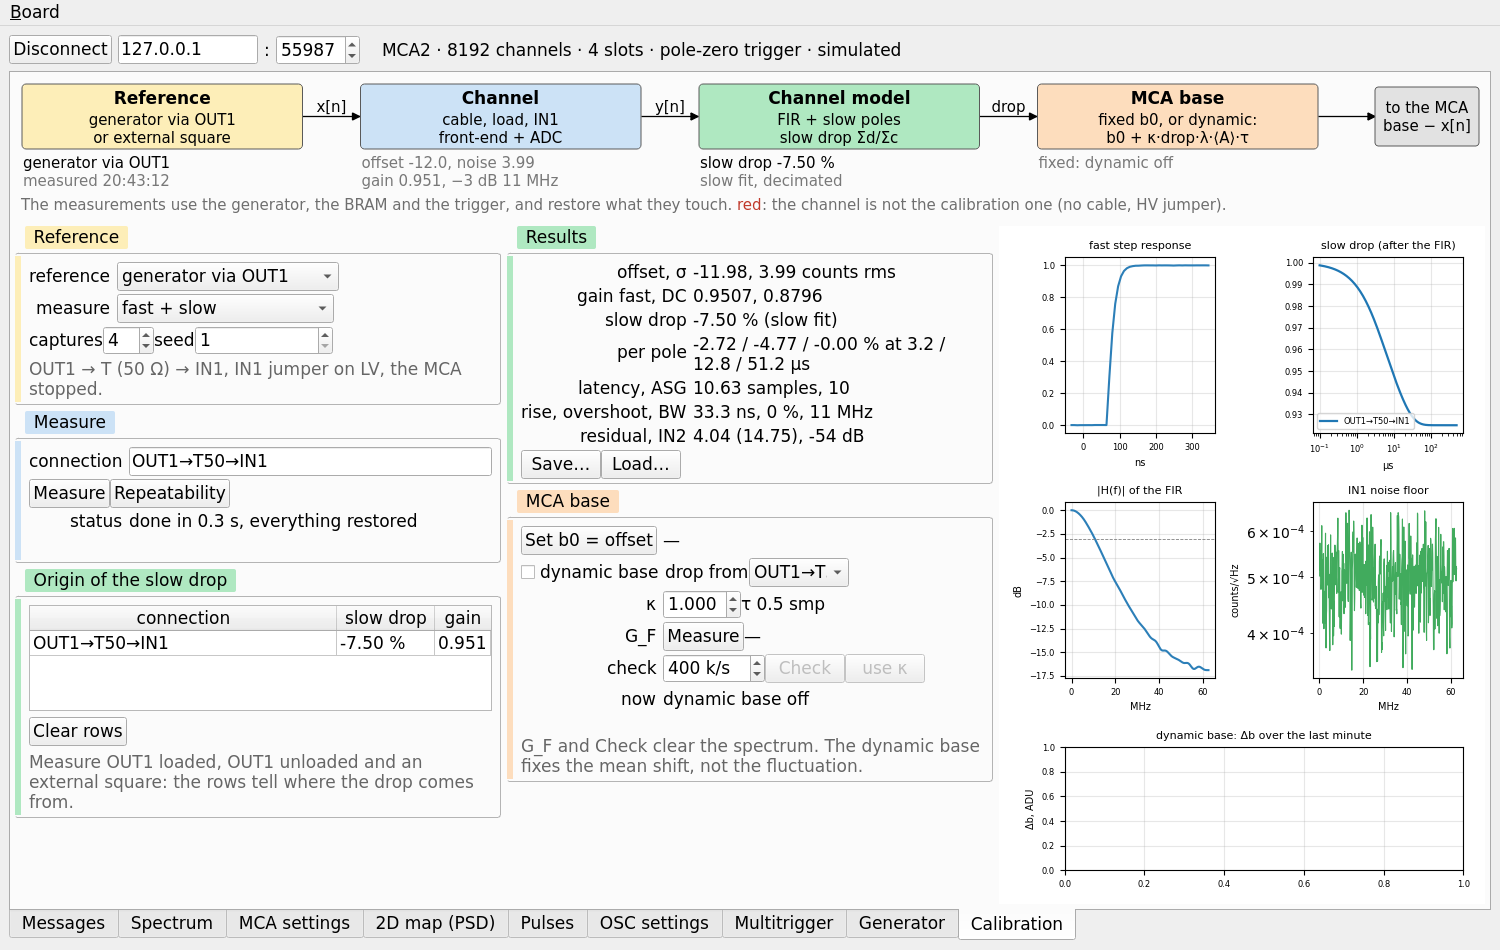
\includegraphics{apD_mcamon_calibration}
\caption[Pestaña \emph{Calibration}]{%
Pestaña \emph{Calibration}: la medición del canal analógico con una referencia
conocida, sus resultados, el origen de la caída lenta y la base del
MCA.\label{f:ap-app-calibration}}
\end{figure}

En la Fig.~\ref{f:ap-app-messages} se presenta la pestaña \emph{Messages}, que
registra cada operación y cada error con su hora. En la captura se ven la
conexión al MCA simulado, con la cantidad de canales y si el \emph{bitstream} trae el
mapa 2D, y el arranque de la adquisición. El registro se puede guardar en un
archivo con ``\emph{Save log}…''.

\begin{figure}[H]
\centering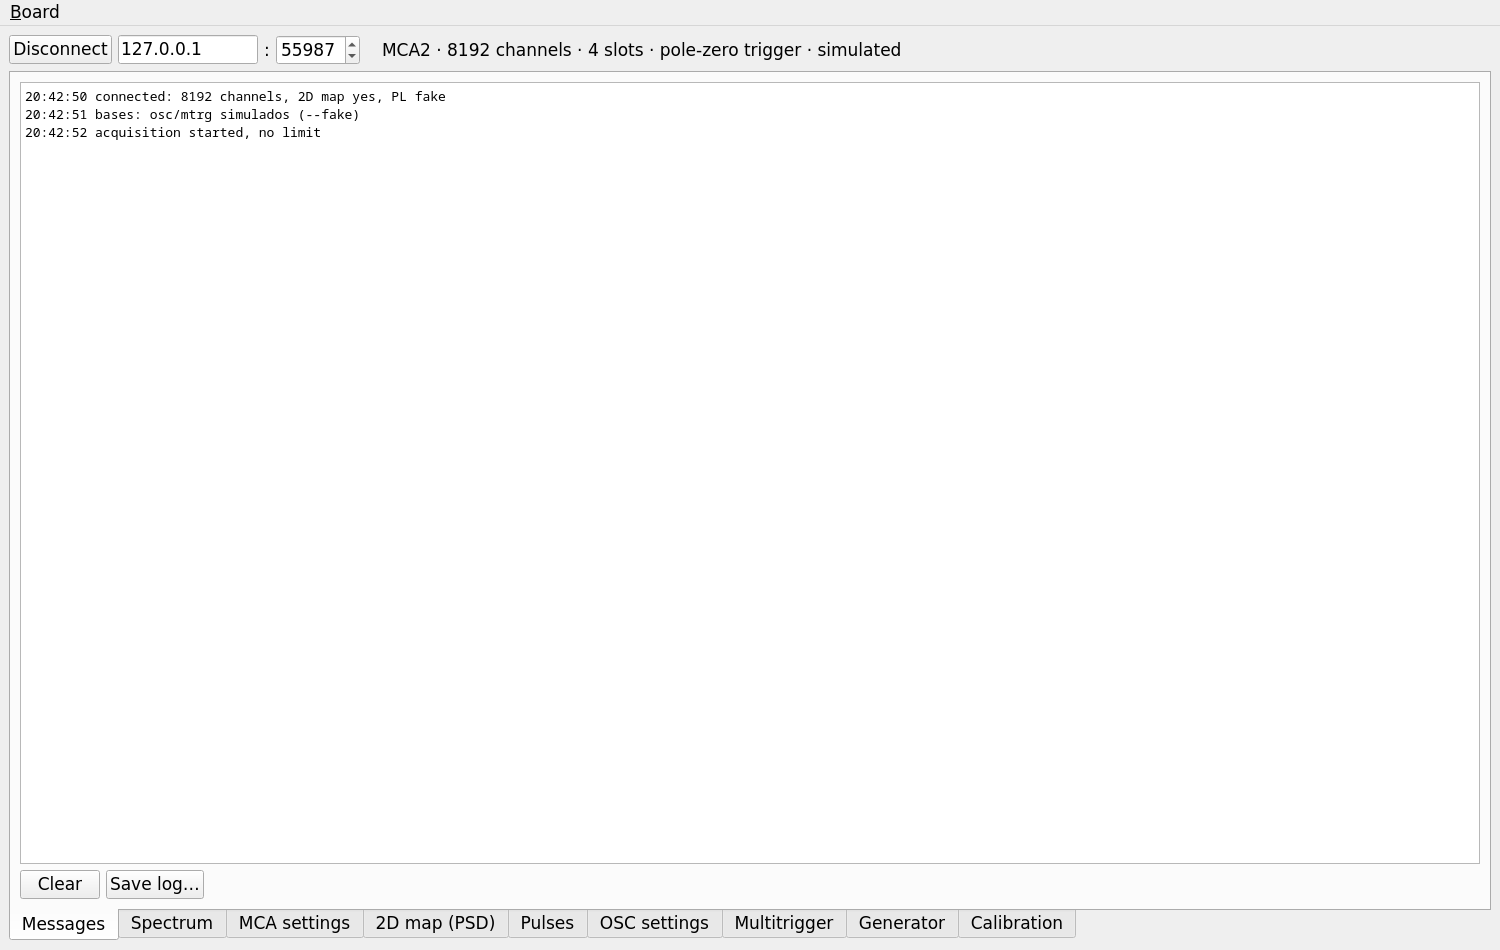
\includegraphics{apD_mcamon_messages}
\caption[Pestaña \emph{Messages}]{%
Pestaña \emph{Messages}: el registro de operaciones y errores, con su
hora.\label{f:ap-app-messages}}
\end{figure}

%%% Local Variables:
%%% mode: latex
%%% TeX-master: "template"
%%% End:
    % Capturas de la aplicación (archivo apend4, apéndice A)
% Origen: sección "Apéndice" de Secciones/PI - Analizador Multicanal.md
\chapter{Complementos del analizador multicanal}
\label{C:ap-mca}

% Figuras de este apéndice + las compartidas.
\graphicspath{{figs/apendices/}{figs/comunes/}}

\section{Posibles detectores empleados}
\label{S:ap-detectores}

En la Tabla~\ref{t:ap-detectores} se presentan algunas de las familias de
detectores con las que se emplea un MCA, la partícula que detectan y los órdenes
de magnitud de sus tiempos característicos, su rango de energía y su tasa de
conteo típica~\cite{Knoll2010}.

\begin{table}[H]
\centering
\caption[Familias de detectores y sus parámetros característicos]{%
Familias de detectores con sus tiempos característicos, rangos de energía y
tasas de conteo típicas.\label{t:ap-detectores}}
\footnotesize
\renewcommand{\arraystretch}{1.3}
\setlength{\tabcolsep}{3pt}
\newcolumntype{Y}{>{\raggedright\arraybackslash}X}
\begin{tabularx}{\textwidth}{|>{\raggedright\arraybackslash}p{0.15\textwidth}|Y|Y|Y|Y|Y|}
\hline
\encabezado \textbf{Detector} & \textbf{Partícula detectada} & \textbf{Tiempo de subida}
  & \textbf{Tiempo de decaimiento / muerto} & \textbf{Rango de energía típico}
  & \textbf{Tasa de conteo típica (orden de magnitud)} \\ \hline
Cámara de ionización
  & $\alpha$, $\beta$, $\gamma$, rayos X, n (con convertidor)
  & \unit{\micro\second} (electrones) -- \unit{\milli\second} (iones)
  & \unit{\milli\second} (cola iónica)
  & \unit{\kilo\electronvolt} -- decenas de \unit{\mega\electronvolt}
  & $10^2$--$10^3$ eventos/s (modo pulso; en modo corriente no aplica) \\ \hline
Contador proporcional
  & $\alpha$, $\beta$, rayos X blandos, n térmicos (BF$_3$, $^3$He)
  & $\sim$\unit{\nano\second} -- cientos de \unit{\nano\second} (electrónica)
  & \unit{\milli\second} si no hay \emph{pulse shaping} CR-RC
  & \unit{\kilo\electronvolt} -- pocos \unit{\mega\electronvolt}
  & $10^4$--$10^5$ eventos/s \\ \hline
Geiger-Müller
  & Cualquier radiación ionizante (sin discriminación)
  & $\sim$\unit{\micro\second}
  & \qtyrange{50}{200}{\micro\second} (tiempo muerto)
  & No espectroscópico
  & $10^3$--$10^4$ eventos/s (saturación por tiempo muerto arriba de esto) \\ \hline
\textbf{Centellador orgánico (plástico, antraceno)}
  & $\beta$, n rápidos (retroceso de protones), $\gamma$ (timing)
  & $\sim$\qtyrange{1}{3}{\nano\second} (plástico), $\sim$\qty{30}{\nano\second} (antraceno)
  & \unit{\nano\second} (decaimiento rápido)
  & \unit{\kilo\electronvolt} -- \unit{\mega\electronvolt}
  & $10^6$--$10^7$ eventos/s \\ \hline
NaI(Tl)
  & $\gamma$, rayos X
  & $\sim$decenas de \unit{\nano\second}
  & $\sim$\qty{230}{\nano\second}
  & \unit{\kilo\electronvolt} -- varios \unit{\mega\electronvolt}
  & $10^5$--$10^6$ eventos/s \\ \hline
CsI(Tl)
  & $\gamma$, rayos X
  & $\sim$decenas de \unit{\nano\second}
  & $\sim$\qty{1000}{\nano\second}
  & \unit{\kilo\electronvolt} -- varios \unit{\mega\electronvolt}
  & $10^4$--$10^5$ eventos/s \\ \hline
LaBr$_3$(Ce)
  & $\gamma$, rayos X
  & $\sim$\unit{\nano\second}
  & \qtyrange{16}{25}{\nano\second}
  & \unit{\kilo\electronvolt} -- varios \unit{\mega\electronvolt}
  & $10^6$--$10^7$ eventos/s \\ \hline
Si (Si(Li), SDD, barrera superficial)
  & $\alpha$, $\beta$, rayos X blandos
  & $\sim$\qtyrange{10}{50}{\nano\second}
  & \unit{\nano\second} -- \unit{\micro\second} (según \emph{shaping})
  & \unit{\kilo\electronvolt} -- pocos \unit{\mega\electronvolt}
  & $10^5$--$10^6$ eventos/s \\ \hline
HPGe
  & $\gamma$ (principalmente)
  & decenas -- cientos de \unit{\nano\second}
  & \unit{\micro\second} (limitado por \emph{shaping} para resolución óptima)
  & \unit{\kilo\electronvolt} -- varios \unit{\mega\electronvolt}
  & $10^4$--$10^5$ eventos/s \\ \hline
CdTe / CZT
  & $\gamma$, rayos X
  & $\sim$decenas -- cientos de \unit{\nano\second}
  & \unit{\nano\second} -- \unit{\micro\second}
  & \unit{\kilo\electronvolt} -- $\sim$\qty{1}{\mega\electronvolt}
  & $10^4$--$10^5$ eventos/s \\ \hline
\end{tabularx}
\end{table}

\section{Aplicaciones del MCA 2D}
\label{S:ap-mca2d}

En la Tabla~\ref{t:ap-mca2d} se presentan las aplicaciones más importantes de
los MCA 2D intracanal.

\begin{table}[H]
\centering
\caption[Principales aplicaciones del MCA 2D intracanal]{%
Principales aplicaciones del MCA 2D intracanal.\label{t:ap-mca2d}}
\small
\renewcommand{\arraystretch}{1.3}
\begin{tabularx}{\textwidth}{|>{\raggedright\arraybackslash}p{0.22\textwidth}|>{\raggedright\arraybackslash}X|>{\raggedright\arraybackslash}p{0.27\textwidth}|}
\hline
\encabezado \textbf{Aplicación} & \textbf{Qué se explota} & \textbf{Requerimientos} \\ \hline
\textbf{Discriminación n/$\gamma$ (PSD)}
  & el centelleador orgánico (EJ-301, BC-501A, estilbeno) da \textbf{colas de
    decaimiento distintas} para protón de retroceso y electrón; los neutrones
    forman un lóbulo propio en el mapa
  & Eje de \emph{fall time} \\ \hline
\textbf{Identificación $\alpha/\beta/\gamma$}
  & Para phoswich, ZnS(Ag)+plástico, CsI(Tl): \textbf{componente rápida/lenta
    distinta por partícula}
  & soportado conceptualmente por el mismo eje \\ \hline
\textbf{Rechazo de colección incompleta de carga}
  & en CdZnTe/HPGe los eventos de mala forma (tiempo de subida largo, eventos
    de superficie) son los que \textbf{fabrican la cola de baja energía} del
    fotopico
  & Eje de \emph{rise time}. \\ \hline
\textbf{Diagnóstico de la propia cadena}
  & deriva de línea base, saturación y déficit balístico mueven o estiran el
    lóbulo; en 1D son invisibles
  & un defecto de la cadena que en 1D pasa inadvertido aparece en el mapa 2D
    como un «pico fantasma» (ver
    Sec.~\ref{S:intro-hw-formal}) \\ \hline
\end{tabularx}
\end{table}

% Las tablas son más largas que el texto: sin el \clearpage flotan detrás de
% las referencias.
\clearpage
% Los apéndices también son \chapter, así que tienen su propia bibliografía.
\bibliografiacapitulo

%%% Local Variables:
%%% mode: latex
%%% TeX-master: "template"
%%% End:
    % Complementos del analizador multicanal
% Origen: sección "Apéndice" de Secciones/PI - Hardware empleado.md
\chapter{Complementos del hardware empleado}
\label{C:ap-hw}

% Figuras de este apéndice + las compartidas.
\graphicspath{{figs/apendices/}{figs/comunes/}}

\section{Criterios de selección de plataforma de HW}
\label{S:ap-hw-criterios}

% Ocupa más de una página: longtable, para que se corte entre filas.
{\small
\begin{longtable}{|>{\raggedright\arraybackslash}p{0.27\textwidth}%
  |>{\raggedright\arraybackslash}p{\dimexpr0.73\textwidth-4\tabcolsep-3\arrayrulewidth\relax}|}
\caption[Criterios de selección de plataforma de HW]{%
Criterios de selección de plataforma de HW. Extraída del
ZynqBook~\citecap{Crockett2014}{4}.\label{t:ap-hw-criterios}} \\
\hline
\encabezado \textbf{Categoría} & \textbf{Factores} \\ \hline
\endfirsthead
\hline
\encabezado \textbf{Categoría} & \textbf{Factores} \\ \hline
\endhead
\textbf{Capacidades del dispositivo} & Rendimiento del procesador\newline
  Rendimiento de la lógica\newline
  Rendimiento de la memoria\newline
  Soporte para aritmética de alta velocidad\newline
  Soporte para E/S y comunicaciones\newline
  Funciones de seguridad y soporte para arranque seguro\newline
  Ancho de banda entre procesador y lógica\newline
  Latencia entre procesador y lógica \\ \hline
\textbf{Factores comerciales} & Lista de materiales (BOM)\newline
  Costos de desarrollo\newline
  Integración (y costos implícitos)\newline
  Longevidad de disponibilidad del dispositivo y soporte técnico\newline
  Calidad y confiabilidad\newline
  Facilidad (costo) de actualizaciones en campo \\ \hline
\textbf{Diseño y desarrollo} & Tiempo de salida al mercado\newline
  Flujos de diseño rápidos, cómodos y confiables\newline
  Verificación integrada\newline
  Integración con otras herramientas de desarrollo\newline
  Soporte para flujos de diseño en equipo\newline
  Soporte para reutilización de diseños\newline
  Soporte para formatos de diseño estándar de la industria\newline
  Soporte para los métodos de entrada de diseño deseados\newline
  Documentación y soporte técnico \\ \hline
\textbf{Características físicas del dispositivo} & Tamaño físico\newline
  Consumo de potencia\newline
  Facilidad de integración y complejidad resultante del PCB\newline
  Conectividad\newline
  Robustez\newline
  Sensibilidad a la radiación\newline
  Rango de temperatura soportado \\ \hline
\textbf{Flexibilidad} & Escalabilidad \emph{(hay dispositivos más grandes y más
  chicos que se pueden adoptar con poco o ningún retrabajo)}\newline
  Portabilidad \emph{(diseños en formatos estándar que se pueden migrar
  desde/hacia otras plataformas)}\newline
  Reprogramabilidad \emph{(capacidad de cambiar la funcionalidad en campo o
  incluso dinámicamente en tiempo de ejecución)}\newline
  Facilidad de particionado \emph{(capacidad de repartir la funcionalidad entre
  hardware y software)}\newline
  Expansibilidad \emph{(facilidad para integrar nueva funcionalidad)} \\ \hline
\end{longtable}}

\section{Detalles de las CLB}
\label{S:ap-hw-clb}

Cada \emph{slice}, a su vez, contiene~\cite{UG474}:
\begin{itemize}
  \item \textbf{4 Look-Up Tables (LUT) de 6 entradas.} Una LUT es una memoria
    SRAM de 64 bits que almacena la tabla de verdad de una función lógica
    arbitraria de hasta 6 variables: configurar la FPGA es, literalmente,
    escribir esas tablas. Cada LUT tiene \textbf{doble salida} (O5/O6) y puede
    usarse como una LUT de 6 entradas o como dos LUT de 5 entradas con las
    entradas compartidas, lo que permite empaquetar dos funciones pequeñas en el
    mismo recurso.
  \item \textbf{8 flip-flops tipo D}, el bloque de memoria mínima sincrónica al
    reloj. Admiten \emph{clock enable} (CE) y \emph{set/reset} (SR). Los 8
    flip-flops de un \emph{slice} comparten el mismo reloj, el mismo CE y el
    mismo SR, esto se suele llamar \emph{control set}. Un diseño con muchos CE
    distintos no puede empaquetar bien y termina ocupando más \emph{slices} de
    los que su cuenta de lógica sugiere.
  \item \textbf{Lógica de acarreo dedicada (CARRY4).} Cuatro bits de cadena de
    acarreo con ruteo propio, vertical y mucho más rápido que la interconexión
    general. Es lo que hace que un sumador en FPGA sea eficiente: sin ella, cada
    acarreo pagaría un salto por la matriz de conmutación.
  \item \textbf{Multiplexores dedicados (F7, F8)}, que combinan las salidas de
    varias LUT para construir funciones de 7 u 8 entradas sin gastar
    interconexión.
\end{itemize}

\section{Detalles de las entradas analógicas rápidas}
\label{S:ap-hw-entradas}

En la Fig.~\ref{f:ap-hw-frontend} aparece el front-end analógico de las entradas
rápidas.

\begin{figure}[H]
\centering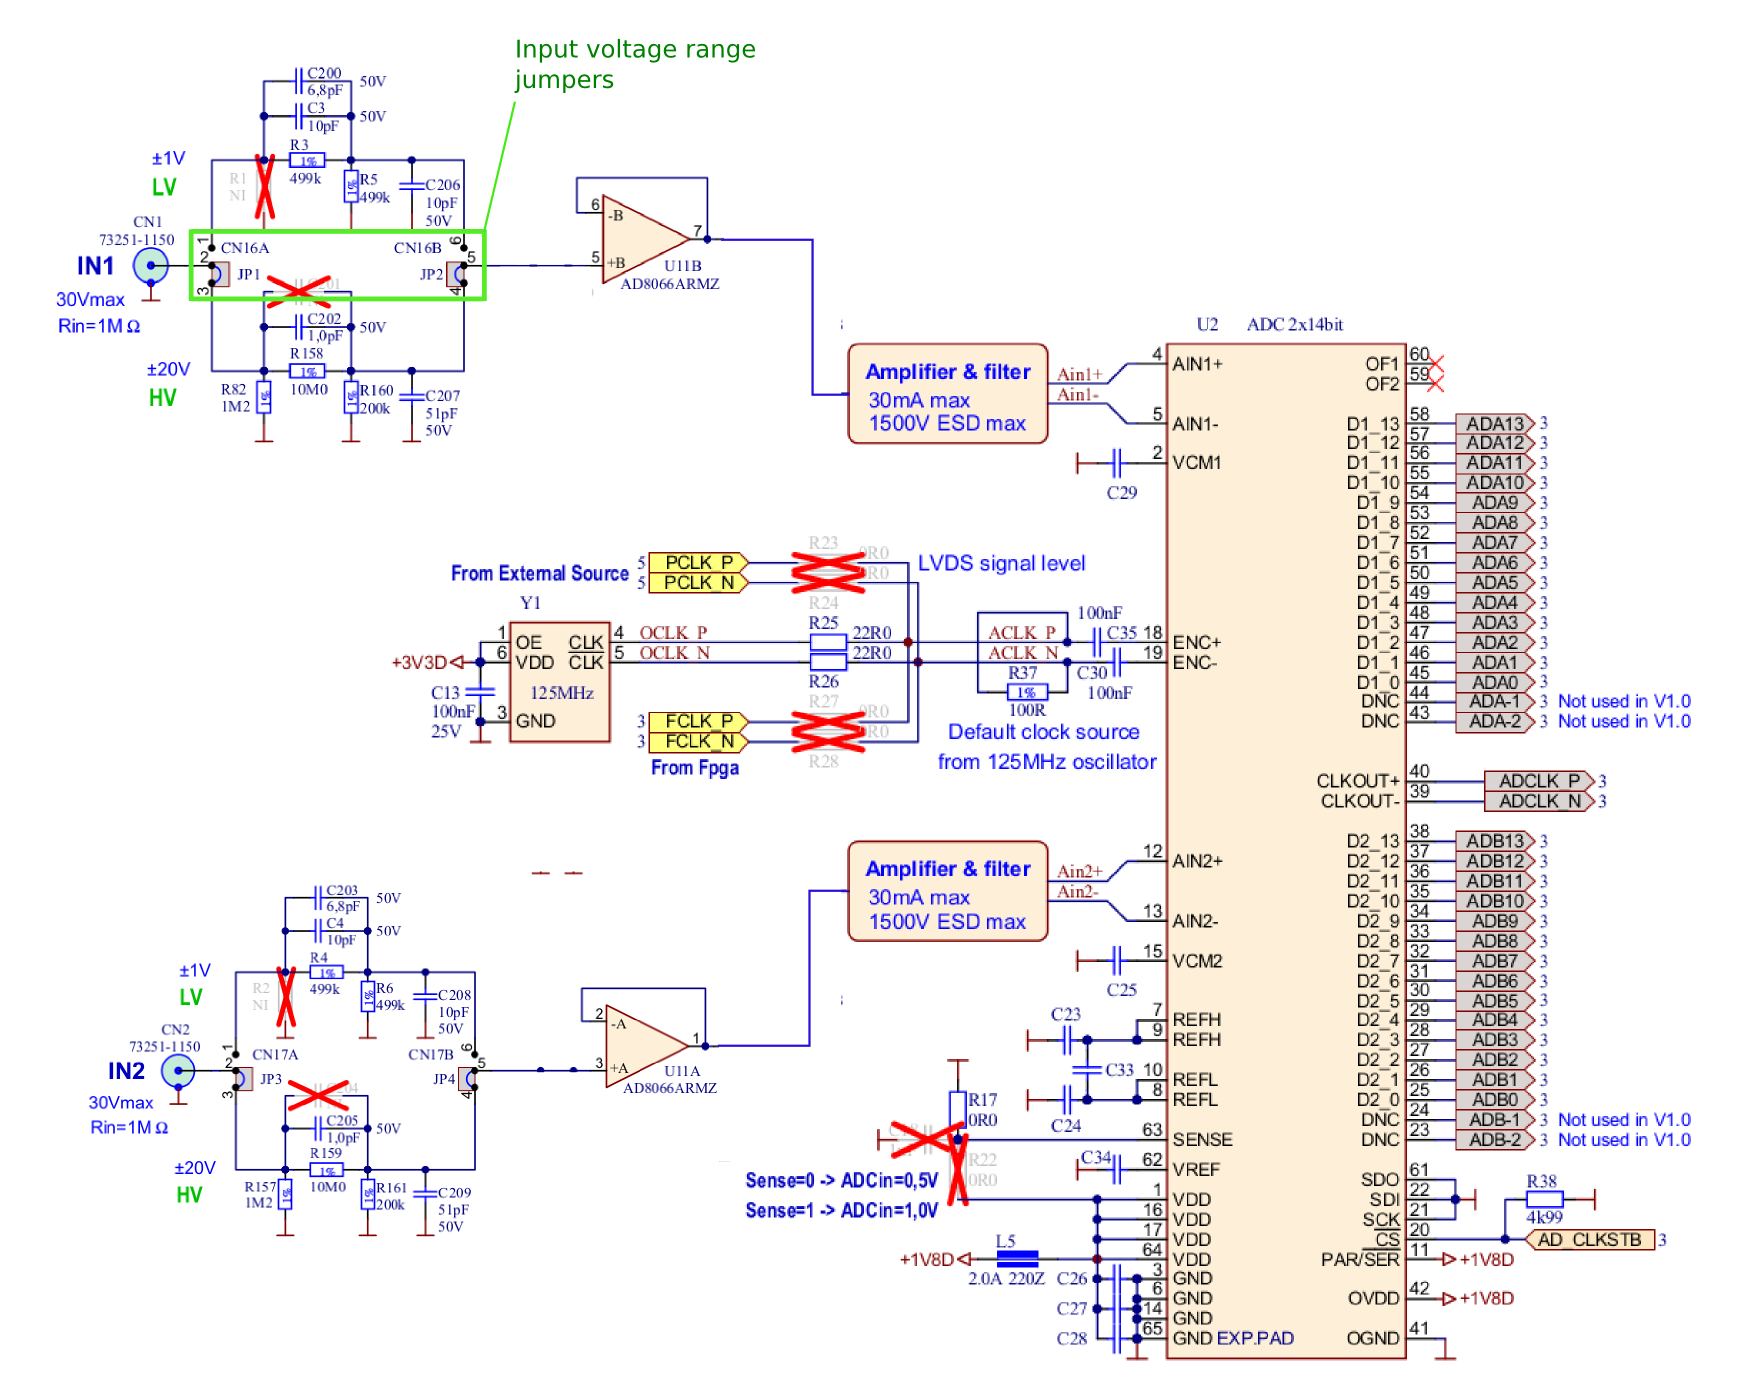
\includegraphics{apB_frontend_pitaya}
\caption[Front-end analógico de las entradas rápidas]{%
Front-end analógico de las entradas de la plataforma: divisor con los jumpers
LV/HV, un buffer (AD8066) y una etapa de amplificación y filtrado antes del ADC.
Extraído del esquemático de Red Pitaya~\cite{RedPitayaSchematics}.
\label{f:ap-hw-frontend}}
\end{figure}

En la Tabla~\ref{t:ap-hw-crosstalk} se presenta la diafonía (\emph{crosstalk})
máxima entre los dos canales de entrada, para cada combinación de jumpers LV/HV.

\begin{table}[H]
\centering
\caption[Diafonía entre los canales IN1 e IN2]{%
Diafonía máxima entre los canales IN1 e IN2 en todas las
configuraciones~\cite{RedPitayaDocs}.\label{t:ap-hw-crosstalk}}
\small
\begin{tabular}{|c|c|c|c|c|}
\hline
\encabezado & \multicolumn{2}{c|}{\textbf{Hasta 30~MHz}}
  & \multicolumn{2}{c|}{\textbf{Por encima de 30~MHz}} \\ \hline
\encabezado \textbf{IN2 \textbackslash{} IN1} & \textbf{LV} & \textbf{HV}
  & \textbf{LV} & \textbf{HV} \\ \hline
\textbf{LV} & $>$55~dB & 50~dB & 40~dB & 40~dB \\ \hline
\textbf{HV} & $>$55~dB & $>$50~dB & $>$40~dB & $>$35~dB \\ \hline
\end{tabular}
\end{table}

En la Fig.~\ref{f:ap-hw-respuesta-in} se presenta la curva de la documentación
oficial de Red Pitaya.

\begin{figure}[H]
\centering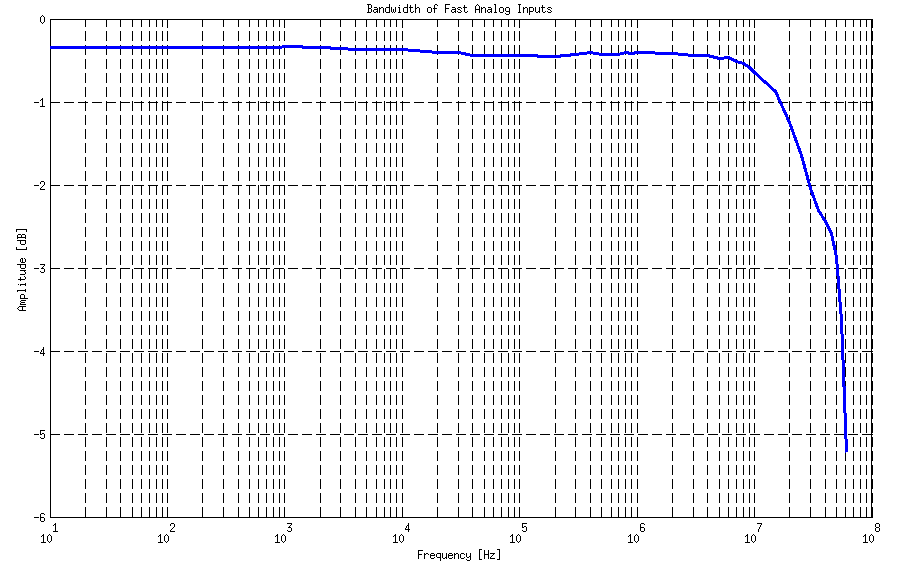
\includegraphics{apB_respuesta_frontend_in}
\caption[Respuesta en frecuencia del front-end de entrada]{%
Módulo de la respuesta en frecuencia del front-end de entrada analógica, de la
documentación de Red Pitaya~\cite{RedPitayaFastIn}. La caída de $-3$~dB está en
aproximadamente 50~MHz.\label{f:ap-hw-respuesta-in}}
\end{figure}

\section{Detalles de la salida analógica rápida: DAC}
\label{S:ap-hw-dac}

La STEMlab 125-14 tiene dos salidas analógicas rápidas, OUT1 y OUT2,
alimentadas por un único conversor digital-analógico (DAC) dual, el AD9767 de
Analog Devices~\cite{AD9767}. Cada salida del conversor pasa por una etapa de
amplificación y filtrado antes del conector SMA (Fig.~\ref{f:ap-hw-dac-etapa}).
En este proyecto OUT1 la maneja el generador de pulsos \codigo{gen\_pulsos}, en
el lugar que dejó libre el generador arbitrario (ASG) de Red Pitaya, para las
pruebas de generación interna por el canal analógico
(Fig.~\ref{f:res-conexion-in-out}).

\begin{figure}[H]
\centering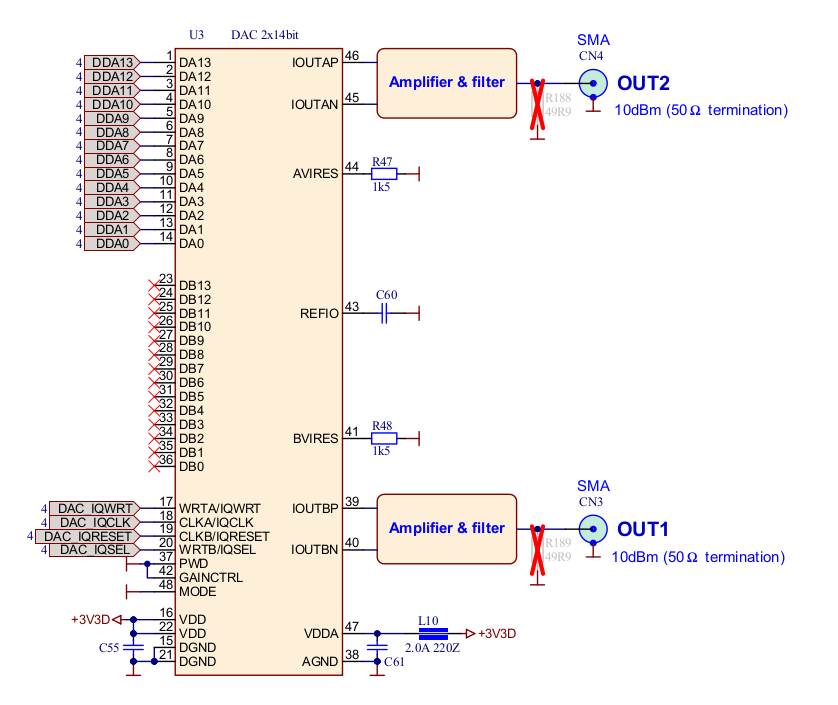
\includegraphics{apB_dac_etapa_salida}
\caption[Conexión del DAC AD9767 en la STEMlab 125-14]{%
Conexión del DAC AD9767 en la STEMlab 125-14, de la documentación de Red
Pitaya~\cite{RedPitayaFastOut}. Las resistencias serie de 49.9~$\Omega$ (R188 y
R189) están sin montar.\label{f:ap-hw-dac-etapa}}
\end{figure}

En la Tabla~\ref{t:ap-hw-salida-rapida} se presentan las características de la
salida según la documentación de Red Pitaya.

\begin{table}[H]
\centering
\caption[Características de las salidas analógicas rápidas]{%
Características de las salidas analógicas rápidas de la STEMlab 125-14, según
la documentación de Red Pitaya~\cite{RedPitayaFastOut}.
\label{t:ap-hw-salida-rapida}}
\small
\begin{tabularx}{\textwidth}{|>{\raggedright\arraybackslash}p{0.27\textwidth}|>{\raggedright\arraybackslash}X|}
\hline
\encabezado & \textbf{Valor} \\ \hline
Canales & 2 (OUT1, OUT2), conector SMA \\ \hline
Tasa de actualización & 125~MS/s por canal \\ \hline
Resolución & 14 bit \\ \hline
Acoplamiento & DC \\ \hline
Rango de salida & ±1~V sobre 50~$\Omega$ \\ \hline
Carga especificada & \textbf{50~$\Omega$}: las salidas sin uso se terminan, y
  una carga de alta impedancia se conecta con una T y 50~$\Omega$ en paralelo
  \\ \hline
Ancho de banda & 50~MHz ($-3$~dB) en la medición; la página de la placa
  declara DC--60~MHz~\cite{RedPitayaDocs} \\ \hline
Límite de \emph{slew rate} & 200~V/µs \\ \hline
Potencia a fondo de escala & $>$~9~dBm; 9.5~dBm típicos con una senoide de
  1~MHz (±1~V de pico sobre 50~$\Omega$ serían 10~dBm) \\ \hline
Armónicos a 8~dBm & $-51$, $-49$, $-48$ y $-53$~dBc a 1, 10, 20 y 45~MHz
  \\ \hline
Errores sin calibrar & offset $<$ 5~\% FS · ganancia $<$ 5~\% \\ \hline
Codificación & offset binary de \textbf{pendiente negativa}, como el ADC: el top
  convierte el complemento a 2 con
  \codigo{\{dac[13], \textasciitilde{}dac[12:0]\}} \\ \hline
Interfaz con la PL & bus paralelo de 14 bits \codigo{LVCMOS33} \\ \hline
\end{tabularx}
\end{table}

Dos números de la tabla limitan los pulsos rápidos. Con 200~V/µs, un escalón de
fondo de escala (2~V) tarda al menos 10~ns, algo más de una muestra, y una
senoide de amplitud $A$ deja de ser lineal por encima de $f = SR/(2\pi A)$: unos
32~MHz para $A = 1$~V. Por eso, según la documentación, el \emph{slew rate} es
el que limita la potencia de salida a fondo de escala. El ancho de banda, por su
parte, redondea los flancos: un sistema de primer orden con su frecuencia de
corte en 50~MHz tiene un tiempo de subida (10--90~\%) de
$0{,}35/f_{-3\,\text{dB}} \approx 7$~ns.

\subsection{El conversor AD9767}
\label{S:ap-hw-ad9767}

El AD9767 es un DAC con salida en corriente. Cada canal entrega un par de
corrientes complementarias, cuya suma es la corriente de fondo de escala
$I_{FS}$. Esa corriente la fijan una resistencia externa $R_{SET}$, en el pin
FSADJ, y la referencia interna de 1.20~V:
\begin{equation}
  I_{FS} = 32\,\frac{V_{REF}}{R_{SET}}, \qquad
  I_{OUTA} = I_{FS}\,\frac{\text{código}}{2^{14}}, \qquad
  I_{OUTB} = I_{FS}\,\frac{2^{14}-1-\text{código}}{2^{14}}
  \label{e:ap-hw-ad9767}
\end{equation}

La etapa de amplificación de la placa convierte esa corriente diferencial en la
tensión de salida. Las características principales del conversor, según su hoja
de datos, se presentan en la Tabla~\ref{t:ap-hw-ad9767}.

\begin{table}[H]
\centering
\caption[Características del DAC AD9767]{%
Características del AD9767 según su hoja de datos~\cite{AD9767}, con
$I_{FS}$~=~20~mA y salida diferencial.\label{t:ap-hw-ad9767}}
\small
\begin{tabularx}{\textwidth}{|>{\raggedright\arraybackslash}p{0.35\textwidth}|>{\raggedright\arraybackslash}X|}
\hline
\encabezado & \textbf{Valor} \\ \hline
Resolución y tasa máxima & 14 bit, 125~MSPS \\ \hline
Salida & corriente complementaria, $I_{FS}$ de 2 a 20~mA \\ \hline
Rango de cumplimiento (\emph{compliance}) & $-1.0$ a $+1.25$~V \\ \hline
INL / DNL a 25~°C & ±1.5 / ±1.0~LSB típicos; ±3.5 / ±2.5~LSB máximos \\ \hline
Apareamiento de ganancia entre canales & ±0.1~\% FSR típico \\ \hline
Establecimiento al 0.1~\% & 35~ns \\ \hline
Subida y bajada (10--90~\%) & 2.5~ns \\ \hline
Impulso de \emph{glitch} & 5~pV$\cdot$s \\ \hline
SFDR a 125~MSPS & 67~dBc con $f_{out}$~=~25~MHz · 70~dBc con 40~MHz \\ \hline
\end{tabularx}
\end{table}

Los 35~ns de establecimiento son unas 4 muestras: un escalón del DAC no queda
dentro del 0.1~\% de su valor final hasta la cuarta o quinta muestra, aparte de
lo que agregue la etapa de salida.

\subsection{Respuesta en frecuencia e impedancia de salida}
\label{S:ap-hw-respuesta-dac}

En la Fig.~\ref{f:ap-hw-dac-respuesta} se presenta la respuesta en frecuencia
de la salida medida por Red Pitaya, con OUT1 a 0~dBm y la otra salida y las dos
entradas terminadas en 50~$\Omega$. Es plana dentro de medio dB hasta unos
35~MHz, con un pequeño sobrepico (+0.3~dB) cerca de 25~MHz, y cae 3~dB en unos
50~MHz.

% Las dos curvas van juntas, lado a lado: por separado la segunda quedaba sola
% en una página al final del apéndice. Cada una mantiene su número y epígrafe.
\begin{figure}[H]
\begin{minipage}[t]{0.49\textwidth}
\captionsetup{width=0.95\linewidth}
\centering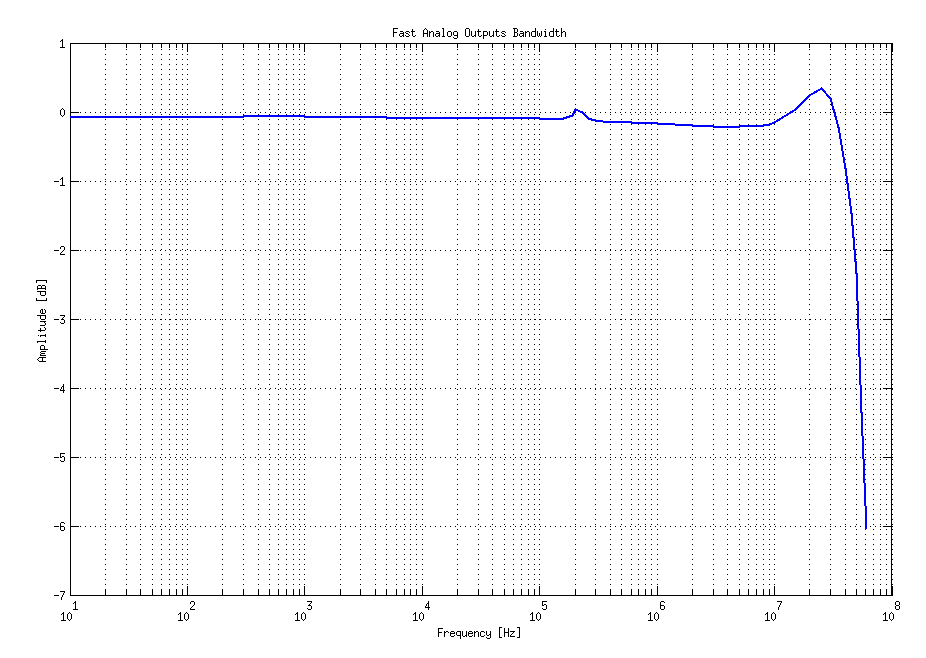
\includegraphics{apB_dac_respuesta_frecuencia}
\caption[Respuesta en frecuencia de las salidas rápidas]{%
Módulo de la respuesta en frecuencia de las salidas rápidas, de la
documentación de Red Pitaya~\cite{RedPitayaFastOut}.
\label{f:ap-hw-dac-respuesta}}
\end{minipage}\hfill
\begin{minipage}[t]{0.49\textwidth}
\captionsetup{width=0.95\linewidth}
\centering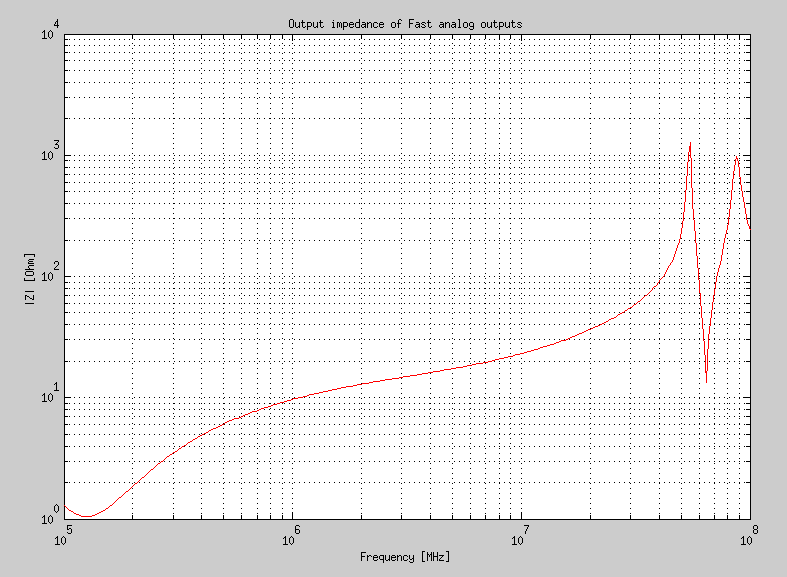
\includegraphics{apB_dac_impedancia}
\caption[Impedancia de salida de las salidas rápidas]{%
Módulo de la impedancia de salida de las salidas rápidas, de la documentación
de Red Pitaya~\cite{RedPitayaFastOut}. El eje horizontal está en Hz.
\label{f:ap-hw-dac-impedancia}}
\end{minipage}
\end{figure}

La salida no es una fuente de 50~$\Omega$: el esquemático prevé una resistencia
serie de 49.9~$\Omega$ por canal (R188 y R189), pero está sin montar. La
impedancia de salida, en la Fig.~\ref{f:ap-hw-dac-impedancia}, es de alrededor
de 1~$\Omega$ a 100~kHz, sube a unos 10~$\Omega$ en 1~MHz y a unos 20~$\Omega$
en 10~MHz, y por encima de los 40~MHz presenta resonancias de hasta
$\sim$1~k$\Omega$. Por eso Red Pitaya pide terminar las salidas en 50~$\Omega$:
con un coaxial sin terminar en el otro extremo, la línea queda desadaptada en
las dos puntas y la señal rebota en el cable. Por la misma razón, la amplitud
sin carga no se duplica, como pasaría con una fuente de 50~$\Omega$.

La caracterización del canal OUT1 $\rightarrow$ IN1 que usamos en las pruebas de
generación interna por el canal analógico se presenta en la
Sec.~\ref{S:res-setup-interna}.

% Las figuras y tablas son más largas que el texto: sin el \clearpage flotan
% detrás de las referencias.
\clearpage
\bibliografiacapitulo

%%% Local Variables:
%%% mode: latex
%%% TeX-master: "template"
%%% End:
    % Complementos del hardware empleado
% Origen: sección "Apéndice" de Secciones/PI - Implementacion Multitrigger.md
% (Detalles de los submódulos, Mapa de memoria y Verificación).
\chapter{Detalles del multitrigger}
\label{C:ap-mt}

% Figuras de este apéndice + las compartidas.
\graphicspath{{figs/apendices/}{figs/comunes/}}

\section{Detalles de los submódulos}
\label{S:ap-mt-submodulos}

A continuación se presentan las decisiones de diseño de los submódulos con
lógica propia. Los puertos, registros y latencias de cada uno están en su hoja
de datos, en \ruta{prj/MCA/docs/datasheet} del repositorio, y el
\emph{ground truth} es el RTL, en \ruta{prj/MCA/modulos/mt}
\textbf{\textcolor{red}{(AGREGAR LINK)}}. En la Fig.~\ref{f:ap-mt-interfaz} se
presenta la interfaz del módulo completo.

\begin{figure}[H]
\centering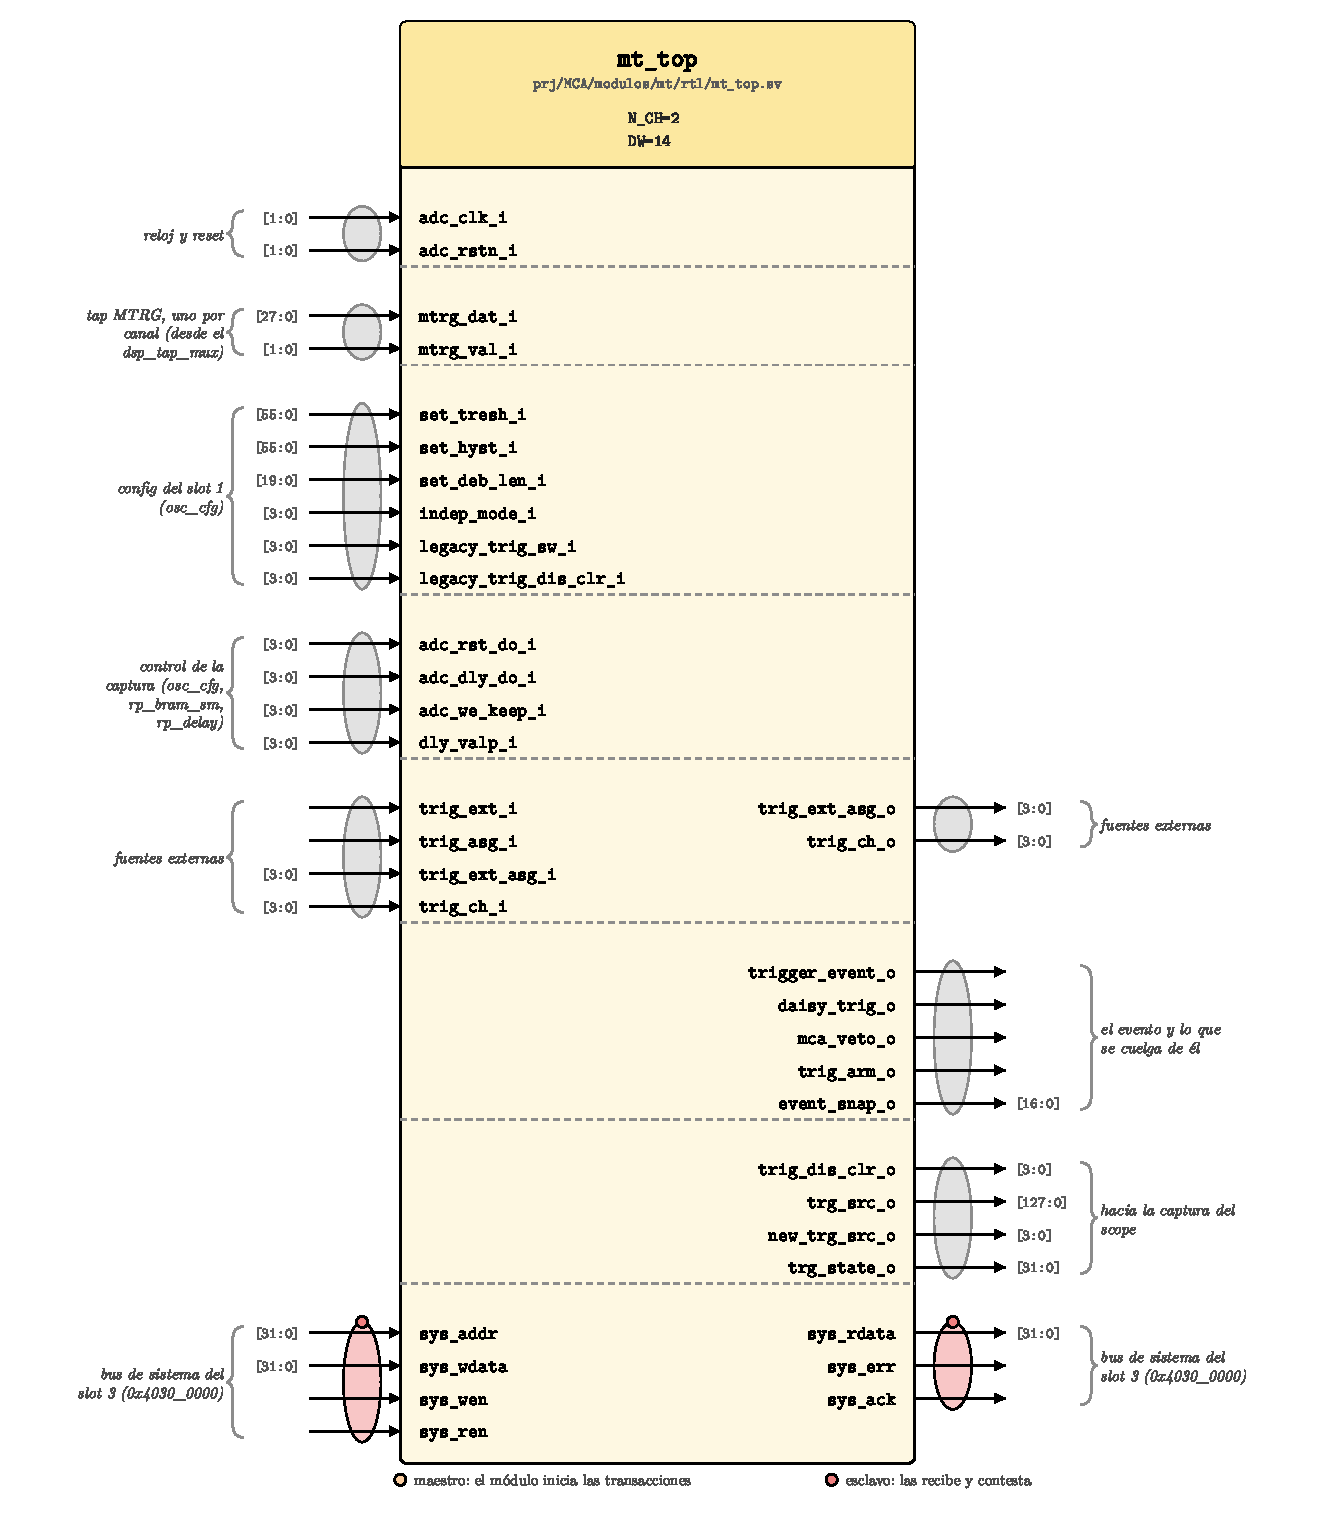
\includegraphics{apC_mt_top_interfaz}
\caption[Interfaz del multitrigger]{%
Interfaz del multitrigger, \codigo{mt\_top}.\label{f:ap-mt-interfaz}}
\end{figure}

\subsection{Disparo por pendiente \texorpdfstring{\texttt{mt\_slope\_trig}}{mt\_slope\_trig}}
\label{S:ap-mt-slope}

Compara el umbral contra una derivada suavizada de la
señal~\cite{Jordanov1994,CAENWP2081}, en lugar de la muestra:
\begin{equation}
  s[n] = \sum_{i=0}^{L-1} x[n-i] - \sum_{i=0}^{L-1} x[n-L-G-i]
  \label{e:ap-mt-slope}
\end{equation}
la suma de las últimas $L$ muestras menos la de $L$ muestras ubicadas $G$ más
atrás. La suma de sus coeficientes es cero, así que una continua da $s = 0$ y el
umbral efectivo no se mueve con la línea de base, como sí le pasa al disparo por
nivel. A la salida tiene un comparador con histéresis simétrico, que da un pulso
por pendiente positiva y otro por negativa.

Se calcula de forma recursiva~\cite{Jordanov1994b},
$s[n] = s[n-1] + (x[n] - x[n-L]) - (x[n-L-G] - x[n-2L-G])$, con tres líneas de
retardo en cascada ($L$, $G$ y $L$ muestras) de una sola toma cada una, que la
síntesis implementa como registros de desplazamiento~\cite{UG474}. Las líneas
avanzan sólo con la muestra válida (\codigo{adc\_dv\_i}), así que el filtro
funciona igual sobre la señal decimada que a 125~MS/s. No tienen \emph{reset}: un
contador \codigo{fill} cuenta las muestras que entraron desde el último
re-arranque, y una toma más vieja que eso lee 0. Así $s$ es exactamente el
filtro aplicado a una señal sin historia previa, y mientras la ventana de
$2L + G$ muestras no se llena no sale ningún pulso.

\begin{figure}[H]
\centering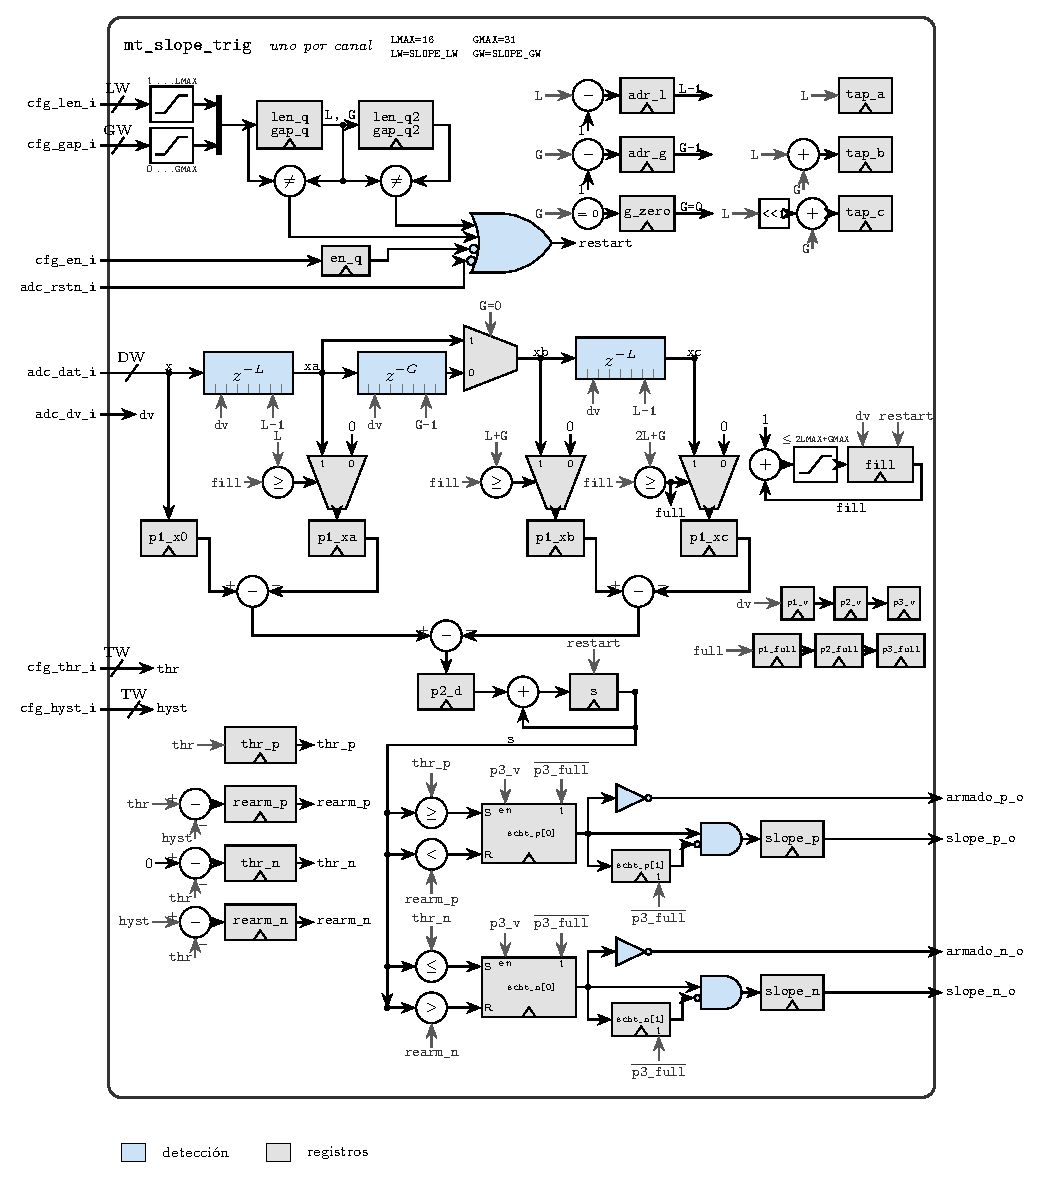
\includegraphics{apC_panorama_mt_slope_trig}
\caption[Implementación del disparo por pendiente]{%
Implementación de \codigo{mt\_slope\_trig}: las tres líneas de retardo, el
cálculo recursivo de $s$ y el comparador con histéresis.\label{f:ap-mt-slope}}
\end{figure}

\subsection{Disparo por polo-cero \texorpdfstring{\texttt{mt\_pz\_trig}}{mt\_pz\_trig}}
\label{S:ap-mt-pz}

Compara el umbral contra la salida de un trapecio corto con cancelación del
polo de la cola~\cite{Jordanov1994,Nakhostin2017}. Es el mismo
\codigo{mca\_trap} del MCA, con subida $k$ y meseta $m$ chicas y las líneas de
retardo en LUT, sin BRAM. Cada pulso sale como un trapecio que vuelve a cero a
las $2k + m$ muestras, apoyado en cero aunque haya una cola debajo. Por eso
separa pulsos cercanos y ve un pulso chico sobre la cola de uno grande, donde la
pendiente queda ciega porque no cancela el polo. El trapecio se presenta en la
Sec.~\refpend{S:implmca-trapezoidal}{Implementación del MCA: recuperación por
conformación trapezoidal}; a la salida tiene el mismo comparador con histéresis
que la pendiente, sólo para pulsos positivos.

\subsection{Escudo \texorpdfstring{\texttt{trigger\_shield}}{trigger\_shield}}
\label{S:ap-mt-shield}

Cuando dispara una fuente habilitada en \codigo{SHIELD\_SRC}, deja inhabilitados
a los destinos de \codigo{SHIELD\_DST} durante un \emph{holdoff} programable, y al
expirar los vuelve a armar. Usa un solo contador para todos los destinos, que se
recarga con cada disparo de una fuente. Fuentes y destinos son vectores
independientes: las fuentes son los disparos de los canales y la entrada
externa (flancos y nivel), y los destinos, los canales y el MCA. Con el mismo
contador resuelve dos cosas: que un canal no se re-dispare con su propio pulso
(Sec.~\ref{S:mt-vulnerabilidades}) y el veto al MCA. Con el nivel externo como
fuente, el veto dura lo que la línea más el \emph{holdoff}.

\begin{figure}[H]
\centering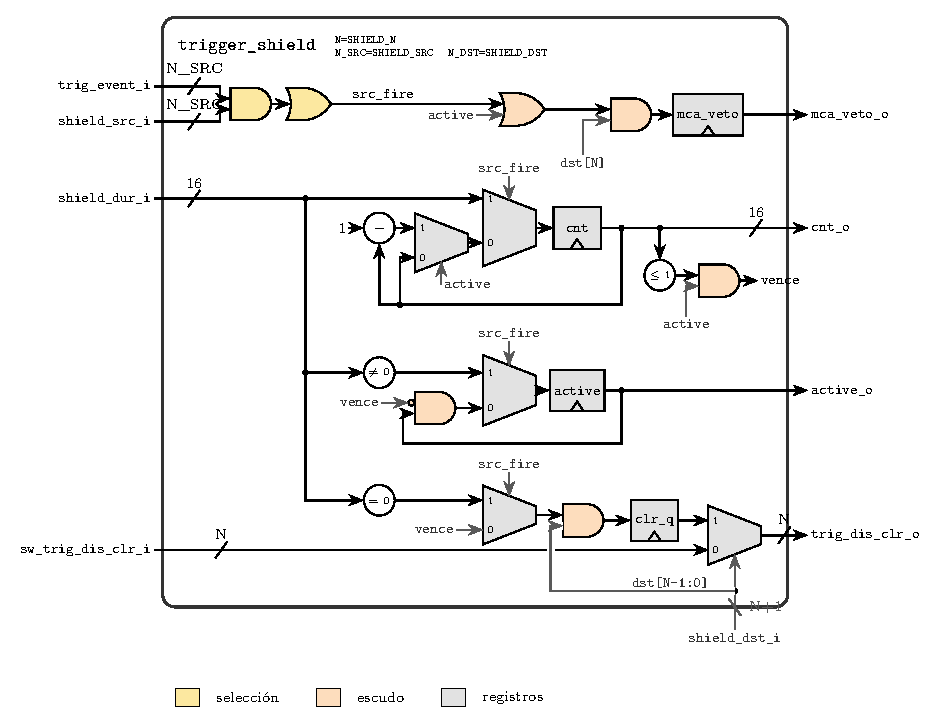
\includegraphics{apC_panorama_trigger_shield}
\caption[Implementación del escudo]{%
Implementación de \codigo{trigger\_shield}: el contador de \emph{holdoff}, el pulso de
re-armado hacia los canales y el veto al MCA.\label{f:ap-mt-shield}}
\end{figure}

\subsection[Selección de fuentes \texttt{mt\_trig\_src} y lógica de eventos \texttt{mt\_event\_logic}]{Selección de fuentes \texorpdfstring{\texttt{mt\_trig\_src}}{mt\_trig\_src}\texorpdfstring{\\}{} y lógica de eventos \texorpdfstring{\texttt{mt\_event\_logic}}{mt\_event\_logic}}
\label{S:ap-mt-src-logica}

\codigo{mt\_trig\_src} y \codigo{mt\_event\_logic} no tienen figura propia: su
estructura se ve en la Fig.~\ref{f:mt-panorama}.

\codigo{mt\_trig\_src} es el selector de un canal. Reemplaza al
\codigo{rp\_trig\_src} original~\cite{RedPitayaFPGA} con dos diferencias: la
máscara es una OR y no un selector de una sola fuente, y la salida va
registrada. Al disparar engancha \codigo{adc\_trg\_dis}, que impide que el
flanco siguiente vuelva a disparar hasta el \emph{clear}, que da el software o el
escudo al expirar su \emph{holdoff}. En \emph{single-shot} además limpia la máscara; en modo
continuo la máscara persiste y alcanza con el \emph{clear}.

\codigo{mt\_event\_logic} no tiene lógica de disparo propia. Instancia un
\codigo{mt\_trig\_src} por canal y el escudo, y saca el evento conjunto
(\codigo{trigger\_event}, la OR de los disparos de los canales),
\codigo{trig\_arm} y el \emph{snapshot} de las fuentes que dispararon el último evento.
El \emph{snapshot} toma las fuentes retrasadas un ciclo, para alinearlas con el
registro de \codigo{mt\_trig\_src}; sin ese retardo guardaría las del ciclo
equivocado.

\subsection{Configuración \texorpdfstring{\texttt{mt\_cfg}}{mt\_cfg}}
\label{S:ap-mt-cfg}

Sigue la estructura del módulo de configuración de la
Sec.~\ref{S:intro-hw-modulo-config}, y sus registros se presentan en la Tabla~\ref{t:ap-mt-mapa}.
Estos registros vivían en el bus del osciloscopio, mezclados con los suyos y
atados a su misma respuesta; pasarlos a un bus propio le da al multitrigger su
propio borde.

\section{Mapa de memoria}
\label{S:ap-mt-mapa}

En la Tabla~\ref{t:ap-mt-mapa} se presentan los registros del multitrigger con
su desplazamiento respecto de la base del módulo. Los registros por canal se repiten cada 4
bytes, de ch0 a ch3. Con todos los registros en su valor de \emph{reset} el módulo no
dispara: el disparo por software también pasa por la máscara (es el bit 0 de
\codigo{OR\_MASK}).

\begin{table}[H]
\centering
\caption[Mapa de registros del multitrigger]{%
Mapa de registros del multitrigger.\label{t:ap-mt-mapa}}
\footnotesize
\setlength{\tabcolsep}{3pt}
\begin{tabularx}{\textwidth}{|>{\raggedright\arraybackslash}p{0.13\textwidth}|c|l|>{\raggedright\arraybackslash}X|>{\raggedright\arraybackslash}p{0.15\textwidth}|}
\hline
\encabezado \textbf{\emph{Offset}} & \textbf{Acceso} & \textbf{Registro}
  & \textbf{Contenido} & \textbf{\emph{Reset}} \\ \hline
\codigo{0x000} & R & \codigo{MAGIC}
  & \codigo{0x4D545247} (\codigo{\textquotedbl MTRG\textquotedbl}) & constante \\ \hline
\codigo{0x004} & R & \codigo{CAPS}
  & \codigo{\{HAS\_PZ[17], HAS\_SLOPE[16], SHIELD\_N[15:12], SRC\_W[11:4],
    N\_CH[3:0]\}} & constante \\ \hline
\codigo{0x010} & RW & \codigo{SHIELD\_CFG}
  & \codigo{\{dur[31:16], dst[12:8], src[6:0]\}} & \codigo{0}, escudo apagado
  \\ \hline
\codigo{0x014} & R & \codigo{SHIELD\_STAT}
  & \codigo{\{trig\_arm[18], mca\_veto[17], active[16], cnt[15:0]\}}
  & \codigo{0} \\ \hline
\codigo{0x018} & R & \codigo{SNAPSHOT}
  & fuentes que dispararon el último evento (29~b) & \codigo{0} \\ \hline
\codigo{0x01C} & R & \codigo{DIS\_FLAGS}
  & \codigo{\{we\_keep[7:4], dis\_act[3:0]\}} & \codigo{0} \\ \hline
\codigo{0x020} & W & \codigo{TRIG\_SW}
  & disparo por software, un bit por canal & lee \codigo{0} \\ \hline
\codigo{0x024} & W & \codigo{TRIG\_DIS\_CLR}
  & \emph{clear} del enganche, un bit por canal & lee \codigo{0} \\ \hline
\codigo{0x028} & R & \codigo{TRG\_STATE}
  & máscara activa, 8~b por canal & \codigo{0} \\ \hline
\codigo{0x040}~+~4$\cdot$ch & RW & \codigo{OR\_MASK}
  & máscara OR del canal, un bit por fuente & \codigo{0}, no dispara nada \\ \hline
\codigo{0x060}~+~4$\cdot$ch & RW & \codigo{SLOPE\_CFG}
  & \codigo{\{en[31], G[12:8], L[4:0]\}} & \codigo{0}, apagado \\ \hline
\codigo{0x070}~+~4$\cdot$ch & RW & \codigo{SLOPE\_THR}
  & umbral de la pendiente \codigo{[17:0]} & \codigo{0} \\ \hline
\codigo{0x080}~+~4$\cdot$ch & RW & \codigo{SLOPE\_HYST}
  & histéresis de la pendiente \codigo{[17:0]} & \codigo{0} \\ \hline
\codigo{0x090}~+~4$\cdot$ch & RW & \codigo{PZ\_CFG}
  & \codigo{\{en[31], sh[29:24], m[12:8], k[4:0]\}} & \codigo{0}, apagado \\ \hline
\codigo{0x0A0}~+~4$\cdot$ch & RW & \codigo{PZ\_MQ}
  & constante del polo-cero, $16 M$ \codigo{[19:0]} & \codigo{0} \\ \hline
\codigo{0x0B0}~+~4$\cdot$ch & RW & \codigo{PZ\_THR}
  & umbral del polo-cero \codigo{[17:0]} & \codigo{0} \\ \hline
\codigo{0x0C0}~+~4$\cdot$ch & RW & \codigo{PZ\_HYST}
  & histéresis del polo-cero \codigo{[17:0]} & \codigo{0} \\ \hline
\end{tabularx}
\end{table}

\section{Verificación}
\label{S:ap-mt-verificacion}

En la Tabla~\ref{t:ap-mt-tests} se presentan los \emph{testbenches} del módulo. Los dos
disparos con filtro se comparan contra un modelo de referencia (\emph{golden
model})~\cite{Bergeron2003} en cada ciclo; el resto se verifica con casos
dirigidos, cada uno con su valor esperado. \codigo{tb\_mt\_top} prueba el módulo
entero a través de su borde, es decir, el cableado entre los submódulos.

\begin{table}[H]
\centering
\caption[\emph{Testbenches} del multitrigger]{%
\emph{Testbenches} del multitrigger.\label{t:ap-mt-tests}}
\footnotesize
\setlength{\tabcolsep}{3pt}
\begin{tabularx}{\textwidth}{|>{\raggedright\arraybackslash}p{0.2\textwidth}|>{\raggedright\arraybackslash}X|>{\raggedright\arraybackslash}p{0.2\textwidth}|}
\hline
\encabezado \textbf{\emph{Testbench}} & \textbf{Qué verifica} & \textbf{Referencia} \\ \hline
\codigo{tb\_mt\_slope\_trig} & el filtro y los pulsos por escalón; que ni la
  continua ni una rampa lenta disparen; el re-arranque al cambiar $L$ o $G$; la
  señal de re-armado & modelo de suma directa \\ \hline
\codigo{tb\_mt\_pz\_trig} & el trapecio y el comparador; el arranque con
  continua; el re-arranque; pares de pulsos; la señal decimada; la señal de
  re-armado & modelo del trapecio y del comparador, bit a bit \\ \hline
\codigo{tb\_mt\_trig\_src} & la máscara OR; el enganche \codigo{adc\_trg\_dis}
  y su \emph{clear}; el disparo por software sujeto a \codigo{dly\_valp}; las fuentes
  de pendiente y polo-cero & casos dirigidos \\ \hline
\codigo{tb\_trigger\_shield} & el \emph{holdoff} de fuentes a destinos, con
  \codigo{dur = 0} y con \codigo{dur} $>$ 0 & casos dirigidos \\ \hline
\codigo{tb\_mt\_event\_logic} & \codigo{trigger\_event} como OR de los canales;
  el \emph{snapshot} (enganche, borrado, alineación con el evento); que un
  \codigo{TRIG\_SW} dé un solo evento; \codigo{trig\_arm} con la máscara vacía,
  fuentes fuera de la máscara, el re-armado y el enganche del escudo
  & casos dirigidos \\ \hline
\codigo{tb\_mt\_cfg} & cada registro contra el mapa anterior; los accesos
  heredados del bus del osciloscopio; el \emph{fan-out} entre canales; el contrato del
  bus en todo su espacio de direcciones & mapa de registros anterior \\ \hline
\codigo{tb\_mt\_top} & cada tipo de disparo configurado por registros hasta
  \codigo{trigger\_event} (nivel, pendiente, polo-cero, externo, software,
  cadena); el veto por nivel externo; el modo continuo; el lazo con la captura;
  \codigo{trig\_arm} & casos dirigidos \\ \hline
\end{tabularx}
\end{table}

% Las figuras y tablas son más largas que el texto: sin el \clearpage flotan
% detrás de las referencias.
\clearpage
\bibliografiacapitulo

%%% Local Variables:
%%% mode: latex
%%% TeX-master: "template"
%%% End:
    % Detalles del multitrigger
% Origen: sección "Apendice" de Secciones/PI - Implementacion OSC.md
% Archivo apend6 por orden de creación; en template.tex va después de apend3.
% Lo que en la nota está entre %% (FSM global del ring, detalles de
% empaquetado) no se transcribe.
\chapter{Detalles del osciloscopio}
\label{C:ap-osc}

% Figuras de este apéndice + las compartidas.
\graphicspath{{figs/apendices/}{figs/comunes/}}

\section{Versión básica}
\label{S:ap-osc-basica}

\subsection{FSM de la captura por BRAM}
\label{S:ap-osc-fsm-bram}

\codigo{rp\_bram\_sm} no tiene una máquina de estados explícita: no hay registro
de estado ni un \codigo{case}. Son cuatro bloques \codigo{always} con banderas
que se enganchan entre sí, y el estado queda implícito en el par
(\codigo{adc\_we}, \codigo{adc\_dly\_do}): si se está escribiendo el \emph{buffer} y si
se está dentro del \emph{post-trigger}. Las cuatro combinaciones se alcanzan
(Fig.~\ref{f:ap-osc-fsm-bram}). Las transiciones las disparan el \emph{trigger}
(\codigo{trig}), los comandos del PS (\codigo{arm} y \codigo{rst}), el modo
continuo (\codigo{keep}) y la cuenta regresiva del \emph{post-trigger},
\codigo{adc\_dly\_cnt}, que se carga con el registro \codigo{DLY}.

\begin{figure}[H]
\centering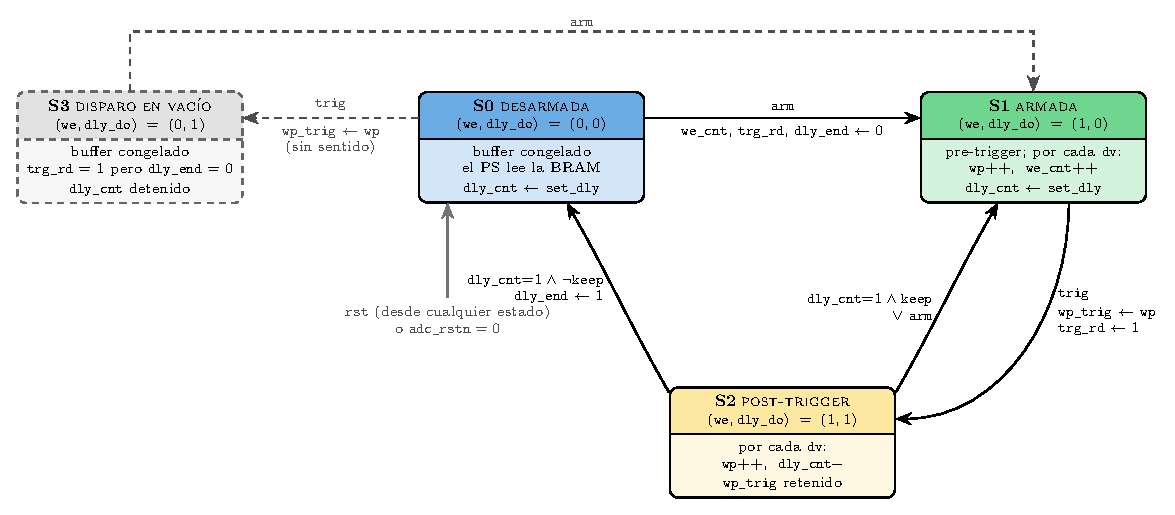
\includegraphics{apOSC_fsm_rp_bram_sm}
\caption[Máquina de estados implícita de \codigo{rp\_bram\_sm}]{%
Máquina de estados implícita de \codigo{rp\_bram\_sm}: el estado es el par
(\codigo{adc\_we}, \codigo{adc\_dly\_do}). S0, S1 y S2 forman el ciclo de
trabajo; S3, con borde punteado, es el camino anómalo de un \emph{trigger} sin armar.
En \codigo{adc\_dly\_do} el \emph{trigger} tiene prioridad sobre \codigo{arm} y
\codigo{rst}, así que un \codigo{arm} y un \codigo{trig} en el mismo ciclo
llevan a S2.\label{f:ap-osc-fsm-bram}}
\end{figure}

\begin{table}[H]
\centering
\caption[Señales de \codigo{rp\_bram\_sm}]{%
Señales de \codigo{rp\_bram\_sm}. Las de estado definen la FSM; las banderas son
\emph{sticky} y se borran sólo con \codigo{arm} o \codigo{rst}. RSZ vale 14 en
el diseño original de RedPitaya y 13 en este proyecto.\label{t:ap-osc-senales-bram}}
\small
\begin{tabularx}{\textwidth}{|l|c|>{\raggedright\arraybackslash}X|l|l|}
\hline \encabezado \textbf{Señal} & \textbf{Ancho} & \textbf{Significado} &
  \textbf{Rol} & \textbf{La lee el PS} \\ \hline
\codigo{adc\_we} & 1 & \textbf{escritura habilitada}; cuando cae, el \emph{buffer}
  queda \textbf{congelado} & estado & \codigo{ADC\_STATE[0]} \\ \hline
\codigo{adc\_dly\_do} & 1 & estamos \textbf{dentro del \emph{post-trigger}} & estado &
  no \\ \hline
\codigo{adc\_dly\_cnt} & 32 & cuenta regresiva del \emph{post-trigger}; se carga con
  \codigo{DLY} & \emph{datapath} & no \\ \hline
\codigo{adc\_dly\_end} & 1 & \emph{sticky}: \textbf{terminó} el \emph{post-trigger} &
  bandera & \codigo{ADC\_STATE[4]} \\ \hline
\codigo{adc\_trg\_rd} & 1 & \emph{sticky}: \textbf{hubo \emph{trigger}} & bandera &
  \codigo{ADC\_STATE[2]} \\ \hline
\codigo{adc\_wp} & RSZ & puntero de escritura; envuelve solo al llegar a
  $2^\text{RSZ}$ & \emph{datapath} & no \\ \hline
\codigo{adc\_wp\_cur} & RSZ & copia registrada de \codigo{adc\_wp} & \emph{datapath} &
  \codigo{WP\_CUR} \\ \hline
\codigo{adc\_wp\_trig} & RSZ & \codigo{adc\_wp} \textbf{capturado en el
  \emph{trigger}} & \emph{datapath} & \codigo{WP\_TRIG} \\ \hline
\codigo{adc\_we\_cnt} & 32 & muestras escritas \textbf{antes} del \emph{trigger}
  (satura) & \emph{datapath} & \codigo{WE\_CNT} \\ \hline
\end{tabularx}
\end{table}

\textbf{Ciclo de trabajo} ($S0\rightarrow S1\rightarrow S2\rightarrow S0$).
Después de un \codigo{rst} la FSM está en S0, con el \emph{buffer} congelado. Un
\codigo{arm} la lleva a S1: \codigo{adc\_we} pasa a 1 y se borran
\codigo{adc\_we\_cnt}, \codigo{adc\_trg\_rd} y \codigo{adc\_dly\_end}. En S1
cada muestra válida se escribe en la BRAM, y avanzan \codigo{adc\_wp} y
\codigo{adc\_we\_cnt}. Un \emph{trigger} la lleva a S2: \codigo{adc\_trg\_rd} pasa a 1,
\codigo{adc\_wp\_trig} guarda dónde cayó el disparo y \codigo{adc\_we\_cnt} deja
de contar. En S2 se siguen escribiendo muestras mientras \codigo{adc\_dly\_cnt}
baja; cuando llega a 1, \codigo{adc\_we} cae, \codigo{adc\_dly\_end} pasa a 1 y
el \emph{buffer} queda congelado ($S2\rightarrow S0$). Ése es el ``terminó'' que el PS
sondea en \codigo{ADC\_STATE}. Dos detalles:
\begin{itemize}
  \item La FSM no espera a que se llene el \emph{pre-trigger}: un \emph{trigger} inmediatamente
    después del \codigo{arm} se acepta, y las muestras anteriores al disparo son
    de la captura anterior. \codigo{adc\_we\_cnt} dice cuántas son válidas, y el
    software lo compara con el pre que pidió.
  \item Con \codigo{DLY = 0} la cuenta nunca vale 1 y \codigo{adc\_we} no cae:
    el \emph{trigger} se registra pero el \emph{buffer} no se congela.
\end{itemize}

\textbf{Modo continuo} (\codigo{keep = 1}). En S2, al terminar la cuenta,
\codigo{adc\_we} sigue en 1 y la FSM vuelve a S1 sin intervención del PS. El
\emph{buffer} nunca se congela: el software detecta los eventos por los cambios de
\codigo{adc\_wp\_trig} y lee memoria que el ADC sigue escribiendo. De ahí viene
el \emph{tearing} de la Sec.~\ref{S:osc-flujo-basico}.

\textbf{Un \codigo{arm} durante el \emph{post-trigger}.} La otra transición
$S2\rightarrow S1$ es un \codigo{arm} en plena captura, y plantea una decisión:
terminar la captura en curso o empezar una nueva. RedPitaya eligió reiniciar.
\codigo{arm} baja \codigo{adc\_dly\_do} y borra las banderas, y la captura
vuelve a empezar desde S1.

\textbf{S3: \emph{trigger} sin armar.} \codigo{adc\_dly\_do} se prende con cualquier
\emph{trigger}, esté o no armada la FSM, así que un \emph{trigger} en S0 la lleva a
S3 = (0, 1). Sus efectos son:
\begin{itemize}
  \item \codigo{adc\_wp\_trig} se sobreescribe con un puntero sin sentido;
  \item \codigo{adc\_trg\_rd} = 1 con \codigo{adc\_dly\_end} = 0, combinación por
    la que el software puede reconocer este estado;
  \item Como \codigo{adc\_dly\_cnt} sólo baja con \codigo{adc\_we} = 1, la FSM
    se queda en S3.
\end{itemize}

Sale con \codigo{arm} (a S1) o con \codigo{rst} (a S0). Con diezmado 1, cada
\emph{trigger} adicional resta uno a la cuenta y puede devolverla sola a S0. El
\codigo{arm} la saca, pero el disparo ya se gastó: es la carrera entre el armado
y el \emph{trigger}.

\section{Regmap de la versión con anillo de eventos}
\label{S:ap-osc-regmap}

En la Tabla~\ref{t:ap-osc-regmap} se presenta el mapa de registros del
\codigo{event\_ring\_top}, con los desplazamientos respecto de la base del
módulo. Todos los registros son de 32 bits y podemos identificar
\textbf{cinco secciones}:
\begin{enumerate}
  \item \textbf{Control y estado} (\codigo{0x00}--\codigo{0x04}).
  \item \textbf{Geometría del anillo} (\codigo{0x08}--\codigo{0x18}): la región
    de DDR y la ventana. Sólo se toman en \codigo{STOPPED}; escritos corriendo
    se ignoran y levantan \codigo{err\_cfg}.
  \item \textbf{Punteros y créditos} (\codigo{0x20}--\codigo{0x2C}).
  \item \textbf{Diagnóstico} (\codigo{0x30}--\codigo{0x50}): contadores de
    descarte, ocupación del \emph{stage} y \emph{timestamp}.
  \item \textbf{Generador de eventos} (\codigo{0x100}--\codigo{0x120}):
    disparos y dato conocido para medir la tasa del anillo sin señal externa.
\end{enumerate}

% Ocupa más de una página: longtable, para que se corte entre filas.
{\small
\begin{longtable}{|l|c|l|>{\raggedright\arraybackslash}p{0.47\textwidth}|l|}
\caption[Regmap del módulo \codigo{event\_ring\_top}]{%
Regmap del módulo \codigo{event\_ring\_top}. Los contadores son libres de 32 bits: las restas entre
lecturas cierran en módulo $2^{32}$.\label{t:ap-osc-regmap}} \\
\hline \encabezado \textbf{\emph{Offset}} & \textbf{Acceso} & \textbf{Nombre} &
  \textbf{Bits / descripción} & \textbf{\emph{Reset}} \\ \hline
\endfirsthead
\hline \encabezado \textbf{\emph{Offset}} & \textbf{Acceso} & \textbf{Nombre} &
  \textbf{Bits / descripción} & \textbf{\emph{Reset}} \\ \hline
\endhead
\codigo{0x00} & W & \codigo{CTRL} & \codigo{[0]} \emph{run}; \codigo{[1]} clr (pulso):
  vacía la cadena y pone en cero \codigo{WR\_SLOT}, \codigo{RD\_SLOT},
  \codigo{SEQ}, los contadores de descarte y eventos, \codigo{err\_cfg} y
  \codigo{err\_fifo\_ovf} & 0 \\ \hline
\codigo{0x00} & R & \codigo{CTRL} & \codigo{[0]} \emph{run} pedido; \codigo{[2:1]}
  estado global & 0 \\ \hline
\codigo{0x04} & R & \codigo{STATUS} & \codigo{[1:0]} estado global (0
  \codigo{STOPPED}, 1 \codigo{RUNNING}, 2 \codigo{DRAINING}); \codigo{[4]}
  \codigo{no\_credit}; \codigo{[5]} \codigo{err\_cfg}; \codigo{[6]}
  \codigo{err\_slot\_ovf}; \codigo{[7]} \codigo{err\_fifo\_ovf} & 0 \\ \hline
\codigo{0x08} & RW & \codigo{SLOT\_BASE} & dirección física del inicio de la
  región de DDR & 0 \\ \hline
\codigo{0x0C} & RW & \codigo{RING\_SZ} & tamaño de la región, en bytes & 0
  \\ \hline
\codigo{0x10} & RW & \codigo{SLOT\_SHIFT} & \codigo{[4:0]} $\log_2$ de los
  bytes por \emph{slot} (mínimo 6) & 9 (512~B) \\ \hline
\codigo{0x14} & RW & \codigo{PRE} & \codigo{[10:0]} muestras antes del \emph{trigger}
  & 8 \\ \hline
\codigo{0x18} & RW & \codigo{POST} & \codigo{[10:0]} muestras desde el \emph{trigger},
  inclusive & 24 \\ \hline
\codigo{0x20} & R & \codigo{WR\_SLOT} & contador libre de \emph{slots} escritos; avanza
  cuando el \codigo{axi\_wr\_fifo} acepta el \emph{footer} & 0 \\ \hline
\codigo{0x24} & RW & \codigo{RD\_SLOT} & contador libre de \emph{slots} leídos; lo
  publica el PS una vez por lote, en cualquier estado & 0 \\ \hline
\codigo{0x28} & R & \codigo{SEQ} & secuencia del próximo evento, la que lleva
  su \emph{footer} & 0 \\ \hline
\codigo{0x2C} & R & \codigo{N\_SLOTS} & \codigo{RING\_SZ
  \textgreater\textgreater{} SLOT\_SHIFT}; derivado, no es un registro & ---
  \\ \hline
\codigo{0x30} & R & \codigo{DROP\_BUSY} & \emph{triggers} durante el drenaje de la
  ventana anterior (tiempo muerto de la PL) & 0 \\ \hline
\codigo{0x34} & R & \codigo{DROP\_FULL} & \emph{triggers} sin lugar aguas abajo
  (tiempo muerto del consumidor) & 0 \\ \hline
\codigo{0x38} & R & \codigo{EV\_CNT} & eventos aceptados por la captura & 0
  \\ \hline
\codigo{0x3C} & R & \codigo{LVL} & \codigo{[2:0]} eventos completos en el
  \emph{stage}; \codigo{[16:4]} muestras en el \emph{stage} & 0 \\ \hline
\codigo{0x40} & R & \codigo{TS\_LO} & \emph{timestamp} \codigo{[31:0]}, en \emph{ticks} desde
  el arranque & 0 \\ \hline
\codigo{0x44} & R & \codigo{TS\_HI} & \emph{timestamp} \codigo{[63:32]} & 0 \\ \hline
\codigo{0x48} & R & \codigo{AXI\_ADDR} & dirección que está escribiendo el
  \codigo{axi\_wr\_fifo} & --- \\ \hline
\codigo{0x50} & R & \codigo{MAGIC} & \codigo{0x45564E54} =
  \codigo{\textquotedbl EVNT\textquotedbl} & --- \\ \hline
\codigo{0x100} & RW & \codigo{GEN\_CTRL} & \codigo{[0]} habilita; \codigo{[1]}
  disparos aleatorios; \codigo{[2]} dato conocido (patrón) en lugar del ADC &
  0 \\ \hline
\codigo{0x104} & RW & \codigo{GEN\_PERIODO} & ciclos entre disparos, modo
  periódico (mínimo 2) & 1000 \\ \hline
\codigo{0x108} & RW & \codigo{GEN\_UMBRAL} & probabilidad de disparo por ciclo
  $\times 2^{32}$, modo aleatorio & 0 \\ \hline
\codigo{0x10C} & RW & \codigo{GEN\_DT\_MIN} & \codigo{[15:0]} ciclos mínimos
  entre disparos, modo aleatorio (mínimo 2) & 2 \\ \hline
\codigo{0x110} & RW & \codigo{GEN\_N} & cantidad de disparos; 0 = sin fin & 0
  \\ \hline
\codigo{0x114} & RW & \codigo{GEN\_SEMILLA} & semilla del generador xorshift;
  0 usa \codigo{0x2545F491} & 0 \\ \hline
\codigo{0x118} & R & \codigo{GEN\_CNT} & disparos emitidos desde el arranque &
  0 \\ \hline
\codigo{0x11C} & R & \codigo{GEN\_ESTADO} & \codigo{[0]} generando;
  \codigo{[1]} llegó a \codigo{GEN\_N} & 0 \\ \hline
\codigo{0x120} & R & \codigo{GEN\_MAGIC} & \codigo{0x47454E31} =
  \codigo{\textquotedbl GEN1\textquotedbl} & --- \\ \hline
\end{longtable}}

% Bibliografía de este apéndice (vacía si no cita nada).
\bibliografiacapitulo

%%% Local Variables:
%%% mode: latex
%%% TeX-master: "template"
%%% End:
    % Detalles del osciloscopio (archivo apend6, apéndice E)
% Origen: sección "Apéndice" de Secciones/PI - Software.md
% Archivo apend5 por orden de creación; en template.tex va después de apend3.
\chapter{Complementos del software}
\label{C:ap-sw}

% Figuras de este apéndice + las compartidas.
\graphicspath{{figs/apendices/}{figs/comunes/}}

\section{Estructuras internas de \texorpdfstring{\texttt{libmca}}{libmca}}
\label{S:ap-sw-estructuras}

En la Tabla~\ref{t:ap-sw-estructuras} se nombran las estructuras internas de
\codigo{libmca}.

\begin{longtable}{|l|>{\raggedright\arraybackslash}p{0.39\textwidth}%
  |>{\raggedright\arraybackslash}p{0.30\textwidth}|}
\caption[Estructuras internas de \codigo{libmca}]{%
Resumen breve de las estructuras internas utilizadas en este
proyecto.\label{t:ap-sw-estructuras}} \\
\hline \encabezado \textbf{Bloque} & \textbf{Estructura} &
  \textbf{Funcionalidad} \\ \hline
\endfirsthead
\hline \encabezado \textbf{Bloque} & \textbf{Estructura} &
  \textbf{Funcionalidad} \\ \hline
\endhead
común & \codigo{mca\_bloque} & base de todo \emph{handle}: el bus y el último error \\ \hline
común & \codigo{mca\_reg\_t} & una fila del mapa de registros \\ \hline
común & \codigo{mca\_field\_t} & una fila de la tabla de campos \\ \hline
bus & \codigo{mca\_bus} & base de los \emph{backends} \\ \hline
bus & \codigo{mca\_bus\_vt} & las funciones de un \emph{backend} \\ \hline
bus & \codigo{devmem\_bus} & \emph{backend} de \codigo{/dev/mem} o de un fichero \\ \hline
bus & \codigo{cb\_bus} & \emph{backend} por \emph{callbacks} \\ \hline
bus & \codigo{mca\_bus\_ops} & las funciones que da quien abre por \emph{callbacks} \\ \hline
DDR & \codigo{mca\_mem} & la región de DDR del ring \\ \hline
MCA & \codigo{mca\_h} & \emph{handle}; guarda la geometría leída al abrir \\ \hline
MCA & \codigo{mca\_info\_t} & qué trae el \emph{bitstream} \\ \hline
MCA & \codigo{mca\_config\_t} & toda la configuración \\ \hline
MCA & \codigo{mca\_forma\_t} & una forma del banco de trapecios \\ \hline
MCA & \codigo{mca\_counters\_t} & contadores y tiempos \\ \hline
MCA & \codigo{mca\_last\_event\_t} & el último evento medido \\ \hline
TOP & \codigo{integration\_h} & \emph{handle}, sin estado propio \\ \hline
TOP & \codigo{integration\_info\_t} & versión y \emph{hash} del \emph{bitstream} \\ \hline
TOP & \codigo{integration\_modules\_t} & qué módulos trae \\ \hline
TOP & \codigo{integration\_slots\_t} & el \emph{slot} de cada módulo \\ \hline
TOP & \codigo{integration\_caps\_t} & la geometría publicada \\ \hline
TOP & \codigo{integration\_route\_t} & de dónde toma la señal un consumidor \\ \hline
TOP & \codigo{integration\_status\_t} & el PLL y el \emph{reset} del ADC \\ \hline
multitrigger & \codigo{multitrigger\_h} & \emph{handle}, sin estado propio \\ \hline
multitrigger & \codigo{multitrigger\_shield\_t} & el \codigo{trigger\_shield} \\ \hline
multitrigger & \codigo{multitrigger\_slope\_t} & el disparo por pendiente \\ \hline
multitrigger & \codigo{multitrigger\_pz\_t} & el disparo con polo-cero \\ \hline
multitrigger & \codigo{multitrigger\_status\_t} & el estado en vivo \\ \hline
osciloscopio & \codigo{osciloscope\_h} & \emph{handle}; guarda la geometría \\ \hline
osciloscopio & \codigo{osciloscope\_geometria\_t} & \codigo{RSZ}, \codigo{N\_CH}, \codigo{DW} y las aperturas \\ \hline
osciloscopio & \codigo{osciloscope\_calib\_t} & la calibración en la PL \\ \hline
osciloscopio & \codigo{osciloscope\_status\_t} & las FSM y los punteros \\ \hline
osciloscopio & \codigo{osciloscope\_adc\_cal\_t} & la calibración de librp, de la EEPROM \\ \hline
osciloscopio & \codigo{osc\_cal\_t} & esa calibración, lista para aplicar \\ \hline
lazo de la BRAM & \codigo{osciloscope\_lote\_cfg\_t} & la configuración de la corrida \\ \hline
lazo de la BRAM & \codigo{osciloscope\_lote\_estado\_t} & lo que sigue entre llamadas \\ \hline
lazo de la BRAM & \codigo{osciloscope\_lote\_t} & las columnas del lote donde escribe C \\ \hline
lazo de la BRAM & \codigo{osciloscope\_lote\_resultado\_t} & guardados y descartados; también la usa el ring \\ \hline
event\_ring & \codigo{osciloscope\_ring\_h} & \emph{handle}; guarda la DDR y un \emph{slot} \\ \hline
event\_ring & \codigo{osciloscope\_ring\_cfg\_t} & la configuración de la corrida \\ \hline
event\_ring & \codigo{osciloscope\_ring\_geometria\_t} & el \emph{slot} y el anillo, sin tocar el hardware \\ \hline
event\_ring & \codigo{osciloscope\_ring\_estado\_t} & lo que sigue entre llamadas \\ \hline
event\_ring & \codigo{osciloscope\_ring\_lote\_t} & las columnas del lote, más \codigo{ts\_hw} y \codigo{seq} \\ \hline
event\_ring & \codigo{osciloscope\_ring\_contadores\_t} & los contadores del hardware \\ \hline
event\_ring & \codigo{osciloscope\_ring\_medida\_t} & lo que acumula \codigo{medir} \\ \hline
generadores & \codigo{gen\_disparos\_cfg\_t} & los registros del motor de disparos \\ \hline
generadores & \codigo{gen\_estado\_t} & la cuenta y el estado de un generador \\ \hline
generadores & \codigo{gen\_pulsos\_h} & \emph{handle}; guarda el bus de HK \\ \hline
generadores & \codigo{gen\_pulsos\_cfg\_t} & toda la configuración de pulsos \\ \hline
\end{longtable}

\section{Detalle de los hilos de captura}
\label{S:ap-sw-hilos}

La Fig.~\ref{f:ap-sw-hilos-captura} es la Fig.~\ref{f:sw-flujo-sesion} con lo
que pasa adentro de cada hilo: las llamadas a C, quién tiene el GIL en cada
tramo, los mensajes a la PL por evento y el \ruta{.tmp} + \codigo{os.replace}
de cada archivo.

\begin{figure}[H]
\centering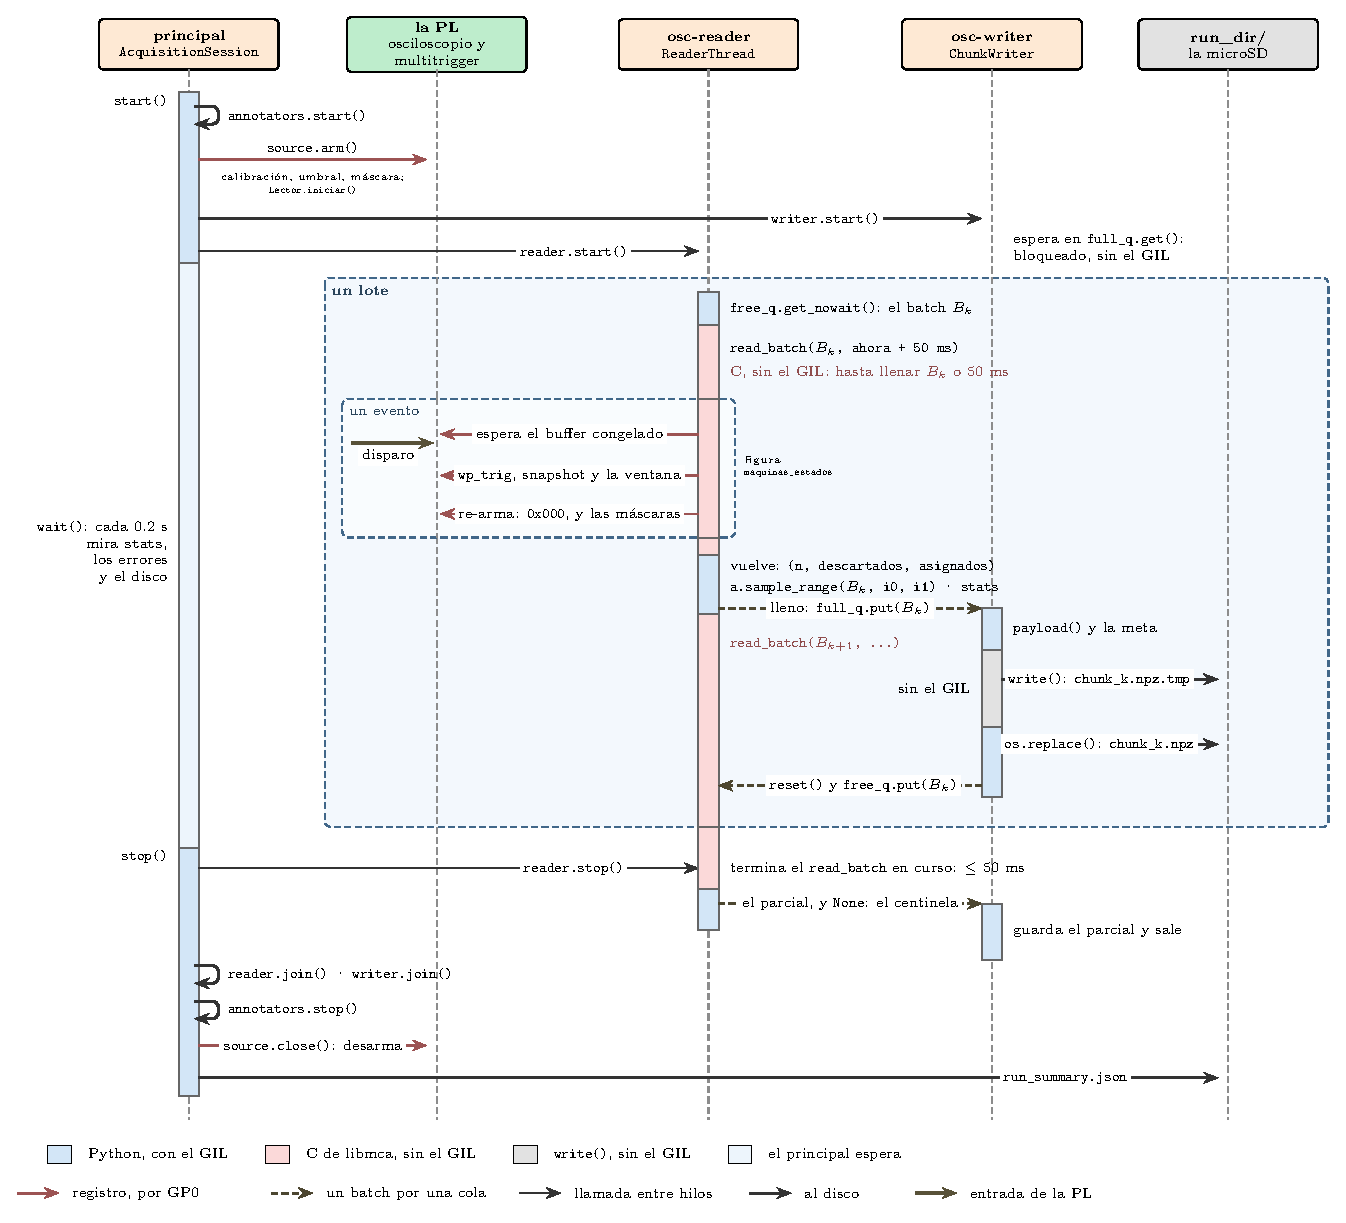
\includegraphics{apE_hilos_captura}
\caption[Detalle de los hilos de captura]{%
Una corrida con \codigo{BramSource}, de \codigo{start()} a \codigo{stop()}, sin
escala. El color sobre cada hilo dice qué corre y si tiene el GIL. El lector
pasa casi todo el tiempo en C (rojo, sin el GIL) y vuelve a Python (azul) una
vez por lote; el escritor pasa su tramo largo en el \codigo{write()} (gris,
también sin el GIL). Por eso no se frenan: el escritor guarda $B_k$ mientras el
lector ya llena $B_{k+1}$. Con \codigo{RingSource} el tramo de C es
\codigo{osciloscope\_ring\_\allowbreak leer\_lote} y los mensajes a la PL son los del ring;
el resto no cambia.\label{f:ap-sw-hilos-captura}}
\end{figure}

\section{Programación del \emph{bitstream}}
\label{S:ap-sw-bitstream}

La utilidad de línea de comandos por defecto de Pitaya simplemente cargaba un
nuevo \emph{bitstream}, independientemente de si este era incorrecto o de si el HW
presente estaba realizando una tarea antes de arrancar. Es así que expandimos la
función original de la carga con tres chequeos; su flujo de utilización se
presenta en la Fig.~\ref{f:ap-sw-bitstream}:
\begin{enumerate}
  \item Comprueba si la versión del Zynq es compatible con el \emph{bitstream}
    presente.
  \item Desactiva/activa las interconexiones AXI mediante puentes del OS.
  \item Implementa un \emph{watchdog} con el que comprueba que el sistema se mantiene
\end{enumerate}

\begin{figure}[H]
\centering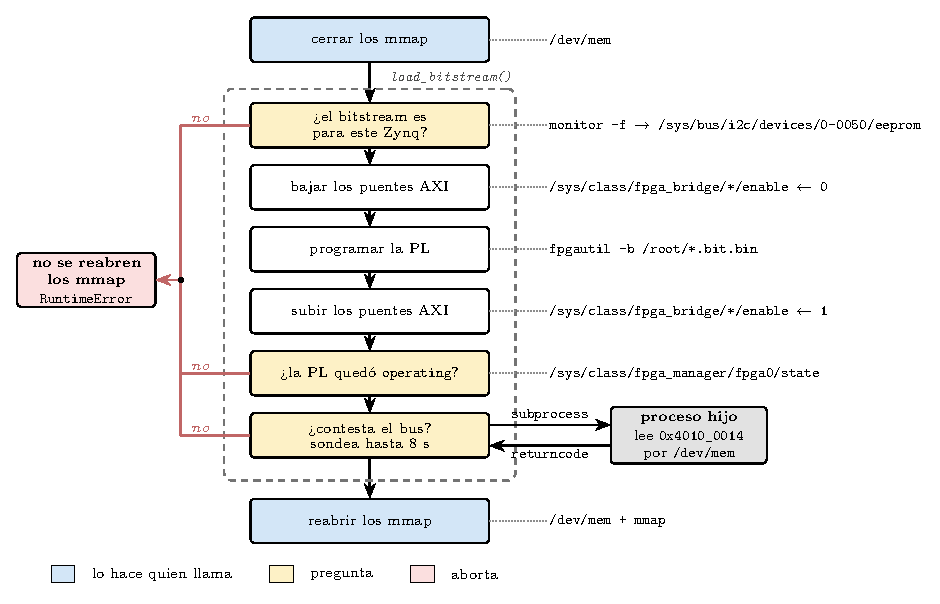
\includegraphics{apE_secuencia_bitstream}
\caption[Carga del \emph{bitstream}]{%
Metodología de la carga del \emph{bitstream} presente.\label{f:ap-sw-bitstream}}
\end{figure}

%%% Local Variables:
%%% mode: latex
%%% TeX-master: "template"
%%% End:
    % Complementos del software (archivo apend5, apéndice F)

%%%%%%%%%%%%%%%%%%%%%%%%%%% Bibliograf\'{\i}a global %%%%%%%%%%%%%%%%%%%%%%%%%%%%%
% Por default NO hay bibliograf\'{\i}a global: cada cap\'{\i}tulo imprime la suya al
% final, con \bibliografiacapitulo (ver cap1.tex / apend1.tex).
%
% Si adem\'{a}s quer\'{e}s una bibliograf\'{\i}a \'{u}nica al final, descomentar el bloque de
% abajo. Advertencia: biblatex no sabe unir refsections, as\'{\i} que la \'{u}nica forma
% de listar todo junto es \nocite{*}, que imprime TODAS las entradas de los .bib,
% incluidas las que no citaste en ning\'{u}n lado. Sirve si mibib.bib contiene
% exactamente tus referencias y nada m\'{a}s.
%
%\begin{biblio}
%\begin{refsection}
%\nocite{*}
%\printbibliography[heading=bibintoc,title=\bibname]
%\end{refsection}
%\end{biblio}


\begin{postliminary}

\begin{seccion}{Agradecimientos}
Agradecimientos
\end{seccion}

\end{postliminary}

\end{document}

